\documentclass[a4paper,11pt]{book}
\usepackage{a4wide}
\usepackage{makeidx}
\usepackage{fancyhdr}
\usepackage{graphicx}
\usepackage{multicol}
\usepackage{float}
\usepackage{textcomp}
\usepackage{alltt}
% \usepackage{times}
\usepackage{ifpdf}

\usepackage[left=1in,right=1in,top=1in,bottom=1in]{geometry}

\ifpdf
\usepackage[pdftex,
            pagebackref=true,
            colorlinks=true,
            linkcolor=blue,
            unicode
           ]{hyperref}
\else
\usepackage[ps2pdf,
            pagebackref=true,
            colorlinks=true,
            linkcolor=blue,
            unicode
           ]{hyperref}
\usepackage{pspicture}
\fi
\usepackage{bookman}
\usepackage[utf8]{inputenc}
\usepackage{doxygen}
\makeindex
\setcounter{tocdepth}{2}
\renewcommand{\footrulewidth}{0.4pt}

\graphicspath{{.}{images/pdfs/}}

\usepackage{color}
\definecolor{linkcol}{rgb}{0,0,0.4} 
\definecolor{citecol}{rgb}{0.5,0,0} 

\hypersetup
{
bookmarksopen=true,
pdftitle="Documentation of magGen",
pdfauthor="Kilmurray - Picco", 
pdfsubject="Generator of Static Evaluators of Multi-plans Attribute Grammars", %subject of the document
pdftoolbar=false, % toolbar hidden
pdfmenubar=true, %menubar shown
pdfhighlight=/l, %effect of clicking on a link
colorlinks=true, %couleurs sur les liens hypertextes
pdfpagemode=None, %aucun mode de page
pdfpagelayout=SinglePage, %ouverture en simple page
pdffitwindow=true, %pages ouvertes entierement dans toute la fenetre
linkcolor=linkcol, %couleur des liens hypertextes internes
citecolor=citecol, %couleur des liens pour les citations
urlcolor=linkcol %couleur des liens pour les url
}

\begin{document}
\begin{titlepage}
\vspace*{7cm}
\begin{center}
{\Huge \textbf{\textit{\sffamily{magGen}}} \\[1ex]\large 1.0 }\\
\vspace*{1cm}
{\large Generated by Doxygen 1.5.8}\\
\vspace*{0.5cm}
{\small{21 July of 2010}}

\end{center}
\end{titlepage}
\clearemptydoublepage
\pagenumbering{roman}
\tableofcontents
\clearemptydoublepage
\pagenumbering{arabic}
\chapter{magGen - Generator of Static Evaluators of Multi-plans Attribute Grammars.}
\label{index}\hypertarget{index}{}magGen: Generator of Static Evaluators for Multi-plans Attribute Grammars.\par
%  \href{http://code.google.com/p/genevalmag/}{\tt http://code.google.com/p/genevalmag/}\par
 Copyright\textcopyright 2010 Kilmurray - Picco\par

\textit{Departamento de Computaci\'on\\
        Facultad de Ciencias Exactas, F\'isico-Qu\'imicas y Naturales\\
        Universidad Nacional de R\'io Cuarto\\
        C\'ordoba - Argentina}

System: magGen\par
 Homepage: $<$\href{http://code.google.com/p/genevalmag/}{\tt http://code.google.com/p/genevalmag/}$>$\par
 Language: C++\par
 \par
%  Authors: Kilmurray, Gerardo Luis\par
%  Authors: Picco, Gonzalo Martín\par
%  E-Mail: gerakilmurray@gmail.com\par
%  E-Mail: gonzalopicco@gmail.com\par
%  \par
 magGen is free software: you can redistribute it and/or modify\par
 it under the terms of the GNU General Public License as published by\par
 the Free Software Foundation, either version 3 of the License, or\par
 (at your option) any later version.\par


 magGen is distributed in the hope that it will be useful,\par
 but WITHOUT ANY WARRANTY; without even the implied warranty of\par
 MERCHANTABILITY or FITNESS FOR A PARTICULAR PURPOSE. See the\par
 GNU General Public License for more details.\par


 You should have received a copy of the GNU General Public License\par
 along with magGen. If not, see $<$\href{http://www.gnu.org/licenses/}{\tt http://www.gnu.org/licenses/}$>$.\par


\begin{Desc}
\item [Director:] Arroyo, Marcelo Daniel
\vspace*{0.8cm}

\item[Author:]Kilmurray, Gerardo Luis $<$\href{mailto:gerakilmurray@gmail.com}{\tt gerakilmurray@gmail.com}$>$ 

Picco, Gonzalo Mart\'in $<$\href{mailto:gonzalopicco@gmail.com}{\tt gonzalopicco@gmail.com}$>$\end{Desc}
\begin{Desc}
\item[Date:]June 2010\end{Desc}
\hypertarget{index_intro}{}\section{Introduction}\label{index_intro}
% Trabajo realizado en el marco de la Tesis de Licenciatura en Ciencias de la Computación.
Work done as part of the Thesis of Bachelor of Computer Science.

SVN repository:\par
\par
$<$\href{http://code.google.com/p/genevalmag/}{\tt http://code.google.com/p/genevalmag/}$>$
\par
% En este repositorio podrá encontrar:\par
In this repository you will find:\par
\begin{itemize}
% \item bin: Contiene el binario de maggen y archivos necesarios para la generación del evaluador.
\item bin: Contains the binary files needed to magGen and evaluator generation.

% \item doc: Contiene toda la documentación y tutoriales de la herramienta.
\item doc: It contains all the documentation and tutorials of the tool.

% \item include: Contiene las cabeceras para incluir los archivos que permiten parsing y analisis de MAG, generación de grafos, planes y secuencias de visitas.
\item include: It contains the headers to include the files that make parsing and analysis of MAG, generating graphs, plans and sequences of visits.

% \item src: Contiene todos los archivos de implementación de la herramienta.
\item src: Contains files for implementing the tool.

% \item examples: Contiene ejemplos para ver el funcionamiento de maggen.
\item examples: It contains examples for operation of maggen.

% \item scripts: Contiene scripts en bash para convertir archivos .dot en imágenes PNG.
\item scripts: Contains bash scripts to convert dot files in PNG images.

\end{itemize}


% Enlaces principales: \href{http://code.google.com/p/genevalmag/}{\tt Genevalmag GoogleCode }

% \hypertarget{index_notes}{}
% \section{Notas}\label{index_notes}
% En etapa de escritura del informe

\hypertarget{index_requirements}{}
\section{Requirements}\label{index_requirements}
% Para compilar la herramienta magGen, se necesita:
To compile maggen tool you need:
\begin{itemize}
\item Boost C++ Libraries >= 1.41 $<$\href{http://www.boost.org/}{\tt http://www.boost.org/}$>$
\item g++ >= 4.3.3
\end{itemize}

\par
\par
 
\chapter{Namespace Index}
\section{Namespace List}
Here is a list of all namespaces with brief descriptions:\begin{CompactList}
\item\contentsline{section}{\hyperlink{namespacegenevalmag}{genevalmag} }{\pageref{namespacegenevalmag}}{}
\item\contentsline{section}{\hyperlink{namespaceutilities}{utilities} }{\pageref{namespaceutilities}}{}
\end{CompactList}

\chapter{Class Hierarchy}
\section{Class Hierarchy}
This inheritance list is sorted roughly, but not completely, alphabetically:\begin{DoxyCompactList}
\item \contentsline{section}{genevalmag::Attr\_\-grammar}{\pageref{classgenevalmag_1_1Attr__grammar}}{}
\item \contentsline{section}{genevalmag::Attribute}{\pageref{classgenevalmag_1_1Attribute}}{}
\item \contentsline{section}{genevalmag::attritute\_\-grammar}{\pageref{structgenevalmag_1_1attritute__grammar}}{}
\item \contentsline{section}{genevalmag::Builder\_\-code}{\pageref{classgenevalmag_1_1Builder__code}}{}
\item \contentsline{section}{genevalmag::Builder\_\-graphs}{\pageref{classgenevalmag_1_1Builder__graphs}}{}
\item \contentsline{section}{genevalmag::Builder\_\-plans}{\pageref{classgenevalmag_1_1Builder__plans}}{}
\item \contentsline{section}{genevalmag::Builder\_\-visit\_\-sequences}{\pageref{classgenevalmag_1_1Builder__visit__sequences}}{}
\item \contentsline{section}{genevalmag::c\_\-rule}{\pageref{structgenevalmag_1_1c__rule}}{}
\item \contentsline{section}{genevalmag::cycle\_\-detector}{\pageref{structgenevalmag_1_1cycle__detector}}{}
\item \contentsline{section}{genevalmag::decl\_\-attribute}{\pageref{structgenevalmag_1_1decl__attribute}}{}
\item \contentsline{section}{genevalmag::attritute\_\-grammar::definition$<$ ScannerT $>$}{\pageref{structgenevalmag_1_1attritute__grammar_1_1definition}}{}
\item \contentsline{section}{genevalmag::skip\_\-parser::definition$<$ ScannerT $>$}{\pageref{structgenevalmag_1_1skip__parser_1_1definition}}{}
\item \contentsline{section}{genevalmag::Equation}{\pageref{classgenevalmag_1_1Equation}}{}
\item \contentsline{section}{genevalmag::Expression}{\pageref{classgenevalmag_1_1Expression}}{}
\begin{DoxyCompactList}
\item \contentsline{section}{genevalmag::Expr\_\-leaf}{\pageref{classgenevalmag_1_1Expr__leaf}}{}
\begin{DoxyCompactList}
\item \contentsline{section}{genevalmag::Expr\_\-instance}{\pageref{classgenevalmag_1_1Expr__instance}}{}
\item \contentsline{section}{genevalmag::Expr\_\-literal}{\pageref{classgenevalmag_1_1Expr__literal}}{}
\end{DoxyCompactList}
\item \contentsline{section}{genevalmag::Expr\_\-node}{\pageref{classgenevalmag_1_1Expr__node}}{}
\begin{DoxyCompactList}
\item \contentsline{section}{genevalmag::Expr\_\-function}{\pageref{classgenevalmag_1_1Expr__function}}{}
\end{DoxyCompactList}
\end{DoxyCompactList}
\item \contentsline{section}{genevalmag::Function}{\pageref{classgenevalmag_1_1Function}}{}
\item \contentsline{section}{genevalmag::i\_\-w}{\pageref{structgenevalmag_1_1i__w}}{}
\item \contentsline{section}{genevalmag::k\_\-p\_\-project}{\pageref{structgenevalmag_1_1k__p__project}}{}
\item \contentsline{section}{genevalmag::k\_\-plan}{\pageref{structgenevalmag_1_1k__plan}}{}
\item \contentsline{section}{genevalmag::k\_\-w}{\pageref{structgenevalmag_1_1k__w}}{}
\item \contentsline{section}{genevalmag::Maglib}{\pageref{classgenevalmag_1_1Maglib}}{}
\item \contentsline{section}{genevalmag::Parser\_\-AG}{\pageref{classgenevalmag_1_1Parser__AG}}{}
\item \contentsline{section}{genevalmag::Rule}{\pageref{classgenevalmag_1_1Rule}}{}
\item \contentsline{section}{genevalmag::Semantics\_\-checks}{\pageref{classgenevalmag_1_1Semantics__checks}}{}
\item \contentsline{section}{genevalmag::skip\_\-parser}{\pageref{structgenevalmag_1_1skip__parser}}{}
\item \contentsline{section}{genevalmag::Sort}{\pageref{classgenevalmag_1_1Sort}}{}
\item \contentsline{section}{genevalmag::Symbol}{\pageref{classgenevalmag_1_1Symbol}}{}
\item \contentsline{section}{genevalmag::vertex\_\-data\_\-t}{\pageref{structgenevalmag_1_1vertex__data__t}}{}
\end{DoxyCompactList}

\chapter{Class Index}
\section{Class List}
Here are the classes, structs, unions and interfaces with brief descriptions:\begin{DoxyCompactList}
\item\contentsline{section}{\hyperlink{classgenevalmag_1_1Attr__grammar}{genevalmag::Attr\_\-grammar} }{\pageref{classgenevalmag_1_1Attr__grammar}}{}
\item\contentsline{section}{\hyperlink{classgenevalmag_1_1Attribute}{genevalmag::Attribute} }{\pageref{classgenevalmag_1_1Attribute}}{}
\item\contentsline{section}{\hyperlink{structgenevalmag_1_1attritute__grammar}{genevalmag::attritute\_\-grammar} }{\pageref{structgenevalmag_1_1attritute__grammar}}{}
\item\contentsline{section}{\hyperlink{classgenevalmag_1_1Builder__code}{genevalmag::Builder\_\-code} }{\pageref{classgenevalmag_1_1Builder__code}}{}
\item\contentsline{section}{\hyperlink{classgenevalmag_1_1Builder__graphs}{genevalmag::Builder\_\-graphs} }{\pageref{classgenevalmag_1_1Builder__graphs}}{}
\item\contentsline{section}{\hyperlink{classgenevalmag_1_1Builder__plans}{genevalmag::Builder\_\-plans} }{\pageref{classgenevalmag_1_1Builder__plans}}{}
\item\contentsline{section}{\hyperlink{classgenevalmag_1_1Builder__visit__sequences}{genevalmag::Builder\_\-visit\_\-sequences} }{\pageref{classgenevalmag_1_1Builder__visit__sequences}}{}
\item\contentsline{section}{\hyperlink{structgenevalmag_1_1c__rule}{genevalmag::c\_\-rule} }{\pageref{structgenevalmag_1_1c__rule}}{}
\item\contentsline{section}{\hyperlink{structgenevalmag_1_1cycle__detector}{genevalmag::cycle\_\-detector} }{\pageref{structgenevalmag_1_1cycle__detector}}{}
\item\contentsline{section}{\hyperlink{structgenevalmag_1_1decl__attribute}{genevalmag::decl\_\-attribute} }{\pageref{structgenevalmag_1_1decl__attribute}}{}
\item\contentsline{section}{\hyperlink{structgenevalmag_1_1attritute__grammar_1_1definition}{genevalmag::attritute\_\-grammar::definition$<$ ScannerT $>$} }{\pageref{structgenevalmag_1_1attritute__grammar_1_1definition}}{}
\item\contentsline{section}{\hyperlink{structgenevalmag_1_1skip__parser_1_1definition}{genevalmag::skip\_\-parser::definition$<$ ScannerT $>$} }{\pageref{structgenevalmag_1_1skip__parser_1_1definition}}{}
\item\contentsline{section}{\hyperlink{classgenevalmag_1_1Equation}{genevalmag::Equation} }{\pageref{classgenevalmag_1_1Equation}}{}
\item\contentsline{section}{\hyperlink{classgenevalmag_1_1Expr__function}{genevalmag::Expr\_\-function} }{\pageref{classgenevalmag_1_1Expr__function}}{}
\item\contentsline{section}{\hyperlink{classgenevalmag_1_1Expr__instance}{genevalmag::Expr\_\-instance} }{\pageref{classgenevalmag_1_1Expr__instance}}{}
\item\contentsline{section}{\hyperlink{classgenevalmag_1_1Expr__leaf}{genevalmag::Expr\_\-leaf} }{\pageref{classgenevalmag_1_1Expr__leaf}}{}
\item\contentsline{section}{\hyperlink{classgenevalmag_1_1Expr__literal}{genevalmag::Expr\_\-literal} }{\pageref{classgenevalmag_1_1Expr__literal}}{}
\item\contentsline{section}{\hyperlink{classgenevalmag_1_1Expr__node}{genevalmag::Expr\_\-node} }{\pageref{classgenevalmag_1_1Expr__node}}{}
\item\contentsline{section}{\hyperlink{classgenevalmag_1_1Expression}{genevalmag::Expression} }{\pageref{classgenevalmag_1_1Expression}}{}
\item\contentsline{section}{\hyperlink{classgenevalmag_1_1Function}{genevalmag::Function} }{\pageref{classgenevalmag_1_1Function}}{}
\item\contentsline{section}{\hyperlink{structgenevalmag_1_1i__w}{genevalmag::i\_\-w} }{\pageref{structgenevalmag_1_1i__w}}{}
\item\contentsline{section}{\hyperlink{structgenevalmag_1_1k__p__project}{genevalmag::k\_\-p\_\-project} }{\pageref{structgenevalmag_1_1k__p__project}}{}
\item\contentsline{section}{\hyperlink{structgenevalmag_1_1k__plan}{genevalmag::k\_\-plan} }{\pageref{structgenevalmag_1_1k__plan}}{}
\item\contentsline{section}{\hyperlink{structgenevalmag_1_1k__w}{genevalmag::k\_\-w} }{\pageref{structgenevalmag_1_1k__w}}{}
\item\contentsline{section}{\hyperlink{classgenevalmag_1_1Maglib}{genevalmag::Maglib} }{\pageref{classgenevalmag_1_1Maglib}}{}
\item\contentsline{section}{\hyperlink{classgenevalmag_1_1Parser__AG}{genevalmag::Parser\_\-AG} }{\pageref{classgenevalmag_1_1Parser__AG}}{}
\item\contentsline{section}{\hyperlink{classgenevalmag_1_1Rule}{genevalmag::Rule} }{\pageref{classgenevalmag_1_1Rule}}{}
\item\contentsline{section}{\hyperlink{classgenevalmag_1_1Semantics__checks}{genevalmag::Semantics\_\-checks} }{\pageref{classgenevalmag_1_1Semantics__checks}}{}
\item\contentsline{section}{\hyperlink{structgenevalmag_1_1skip__parser}{genevalmag::skip\_\-parser} }{\pageref{structgenevalmag_1_1skip__parser}}{}
\item\contentsline{section}{\hyperlink{classgenevalmag_1_1Sort}{genevalmag::Sort} }{\pageref{classgenevalmag_1_1Sort}}{}
\item\contentsline{section}{\hyperlink{classgenevalmag_1_1Symbol}{genevalmag::Symbol} }{\pageref{classgenevalmag_1_1Symbol}}{}
\item\contentsline{section}{\hyperlink{structgenevalmag_1_1vertex__data__t}{genevalmag::vertex\_\-data\_\-t} }{\pageref{structgenevalmag_1_1vertex__data__t}}{}
\end{DoxyCompactList}

\chapter{File Index}
\section{File List}
Here is a list of all files with brief descriptions:\begin{CompactList}
\item\contentsline{section}{include/\hyperlink{Maglib_8h}{Maglib.h} (Header of the library of evaluator's generator )}{\pageref{Maglib_8h}}{}
\item\contentsline{section}{include/Attr\_\-grammar/\hyperlink{Attr__grammar_8h}{Attr\_\-grammar.h} (Class that represent the full attribute grammar )}{\pageref{Attr__grammar_8h}}{}
\item\contentsline{section}{include/Attr\_\-grammar/\hyperlink{Attribute_8h}{Attribute.h} (Class of the attribute of the attribute grammar )}{\pageref{Attribute_8h}}{}
\item\contentsline{section}{include/Attr\_\-grammar/\hyperlink{Equation_8h}{Equation.h} (Class of the equations of the attribute grammar )}{\pageref{Equation_8h}}{}
\item\contentsline{section}{include/Attr\_\-grammar/\hyperlink{Function_8h}{Function.h} (Class of the function of the attribute grammar )}{\pageref{Function_8h}}{}
\item\contentsline{section}{include/Attr\_\-grammar/\hyperlink{Rule_8h}{Rule.h} (Class of the rule of the attribute grammar )}{\pageref{Rule_8h}}{}
\item\contentsline{section}{include/Attr\_\-grammar/\hyperlink{Sort_8h}{Sort.h} (Class of the sort of the attribute grammar )}{\pageref{Sort_8h}}{}
\item\contentsline{section}{include/Attr\_\-grammar/\hyperlink{Symbol_8h}{Symbol.h} (Class of the symbol of the attribute grammar )}{\pageref{Symbol_8h}}{}
\item\contentsline{section}{include/Builders/\hyperlink{Builder__code_8h}{Builder\_\-code.h} (Header with the functions for build the header and source code of the evaluator of MAG )}{\pageref{Builder__code_8h}}{}
\item\contentsline{section}{include/Builders/\hyperlink{Builder__graphs_8h}{Builder\_\-graphs.h} (Header with the functions for build all kind of graphs for the attribute grammar )}{\pageref{Builder__graphs_8h}}{}
\item\contentsline{section}{include/Builders/\hyperlink{Builder__plans_8h}{Builder\_\-plans.h} (Header of generation plans module of Attribute Grammar )}{\pageref{Builder__plans_8h}}{}
\item\contentsline{section}{include/Builders/\hyperlink{Builder__visit__sequences_8h}{Builder\_\-visit\_\-sequences.h} (Header with the functions for build the visits sequences of grammar )}{\pageref{Builder__visit__sequences_8h}}{}
\item\contentsline{section}{include/Expression\_\-tree/\hyperlink{Expr__function_8h}{Expr\_\-function.h} (Function element of an Expression )}{\pageref{Expr__function_8h}}{}
\item\contentsline{section}{include/Expression\_\-tree/\hyperlink{Expr__instance_8h}{Expr\_\-instance.h} (Instance element of an Expression )}{\pageref{Expr__instance_8h}}{}
\item\contentsline{section}{include/Expression\_\-tree/\hyperlink{Expr__leaf_8h}{Expr\_\-leaf.h} (Abstract final element of an Expression )}{\pageref{Expr__leaf_8h}}{}
\item\contentsline{section}{include/Expression\_\-tree/\hyperlink{Expr__literal_8h}{Expr\_\-literal.h} (Literal element of an Expression )}{\pageref{Expr__literal_8h}}{}
\item\contentsline{section}{include/Expression\_\-tree/\hyperlink{Expr__node_8h}{Expr\_\-node.h} (Abstract recursive element of an Expression )}{\pageref{Expr__node_8h}}{}
\item\contentsline{section}{include/Expression\_\-tree/\hyperlink{Expression_8h}{Expression.h} (Abstract expression )}{\pageref{Expression_8h}}{}
\item\contentsline{section}{include/Parser/\hyperlink{Parser__AG_8h}{Parser\_\-AG.h} }{\pageref{Parser__AG_8h}}{}
\item\contentsline{section}{include/Parser/\hyperlink{Semantics__actions_8h}{Semantics\_\-actions.h} (Header semantics actions for parse of Attribute grammar )}{\pageref{Semantics__actions_8h}}{}
\item\contentsline{section}{include/Parser/\hyperlink{Semantics__checks_8h}{Semantics\_\-checks.h} (Header method Semantics checks of Attribute grammar )}{\pageref{Semantics__checks_8h}}{}
\item\contentsline{section}{include/Util/\hyperlink{Utilities_8h}{Utilities.h} (Header of \hyperlink{namespaceutilities}{utilities} module, where are methods and function used by many class )}{\pageref{Utilities_8h}}{}
\item\contentsline{section}{src/\hyperlink{maggen_8cpp}{maggen.cpp} (Tool for Generation of Static Evaluators for Multi-plans Attribute Grammars.)}
{\pageref{maggen_8cpp}}{}
\item\contentsline{section}{src/\hyperlink{Maglib_8cpp}{Maglib.cpp} (Implementation of the library of evaluator's generator )}{\pageref{Maglib_8cpp}}{}
\item\contentsline{section}{src/Attr\_\-grammar/\hyperlink{Attr__grammar_8cpp}{Attr\_\-grammar.cpp} (Implementation of the methods the \hyperlink{Attr__grammar_8h}{Attr\_\-grammar.h} )}{\pageref{Attr__grammar_8cpp}}{}
\item\contentsline{section}{src/Attr\_\-grammar/\hyperlink{Attribute_8cpp}{Attribute.cpp} (Implementation of the methods the \hyperlink{Attribute_8h}{Attribute.h} )}{\pageref{Attribute_8cpp}}{}
\item\contentsline{section}{src/Attr\_\-grammar/\hyperlink{Equation_8cpp}{Equation.cpp} (Implementation of the methods the \hyperlink{Equation_8h}{Equation.h} )}{\pageref{Equation_8cpp}}{}
\item\contentsline{section}{src/Attr\_\-grammar/\hyperlink{Function_8cpp}{Function.cpp} (Implementation of the methods the \hyperlink{Function_8h}{Function.h} )}{\pageref{Function_8cpp}}{}
\item\contentsline{section}{src/Attr\_\-grammar/\hyperlink{Rule_8cpp}{Rule.cpp} (Implementation of the methods the \hyperlink{Rule_8h}{Rule.h} )}{\pageref{Rule_8cpp}}{}
\item\contentsline{section}{src/Attr\_\-grammar/\hyperlink{Sort_8cpp}{Sort.cpp} (Implementation of the methods the \hyperlink{Sort_8h}{Sort.h} )}{\pageref{Sort_8cpp}}{}
\item\contentsline{section}{src/Attr\_\-grammar/\hyperlink{Symbol_8cpp}{Symbol.cpp} (Implementation of the methods the \hyperlink{Symbol_8h}{Symbol.h} )}{\pageref{Symbol_8cpp}}{}
\item\contentsline{section}{src/Builders/\hyperlink{Builder__code_8cpp}{Builder\_\-code.cpp} (Implementation of the methods the \hyperlink{Builder__code_8h}{Builder\_\-code.h} )}{\pageref{Builder__code_8cpp}}{}
\item\contentsline{section}{src/Builders/\hyperlink{Builder__graphs_8cpp}{Builder\_\-graphs.cpp} (Implementation of the methods the Builder\_\-graph.h )}{\pageref{Builder__graphs_8cpp}}{}
\item\contentsline{section}{src/Builders/\hyperlink{Builder__plans_8cpp}{Builder\_\-plans.cpp} (Implementation of the methods the \hyperlink{Builder__plans_8h}{Builder\_\-plans.h} )}{\pageref{Builder__plans_8cpp}}{}
\item\contentsline{section}{src/Builders/\hyperlink{Builder__visit__sequences_8cpp}{Builder\_\-visit\_\-sequences.cpp} }{\pageref{Builder__visit__sequences_8cpp}}{}
\item\contentsline{section}{src/Expression\_\-tree/\hyperlink{Expr__function_8cpp}{Expr\_\-function.cpp} (Implementation of a function element of an Expression )}{\pageref{Expr__function_8cpp}}{}
\item\contentsline{section}{src/Expression\_\-tree/\hyperlink{Expr__instance_8cpp}{Expr\_\-instance.cpp} (Implementation of a instance element of an Expression )}{\pageref{Expr__instance_8cpp}}{}
\item\contentsline{section}{src/Expression\_\-tree/\hyperlink{Expr__leaf_8cpp}{Expr\_\-leaf.cpp} (Implementation element of an Expression )}{\pageref{Expr__leaf_8cpp}}{}
\item\contentsline{section}{src/Expression\_\-tree/\hyperlink{Expr__literal_8cpp}{Expr\_\-literal.cpp} (Implementation of a literal element of an Expression )}{\pageref{Expr__literal_8cpp}}{}
\item\contentsline{section}{src/Expression\_\-tree/\hyperlink{Expr__node_8cpp}{Expr\_\-node.cpp} (Implementation element of an Expression )}{\pageref{Expr__node_8cpp}}{}
\item\contentsline{section}{src/Expression\_\-tree/\hyperlink{Expression_8cpp}{Expression.cpp} (Implementation of an Expression )}{\pageref{Expression_8cpp}}{}
\item\contentsline{section}{src/Parser/\hyperlink{Parser__AG_8cpp}{Parser\_\-AG.cpp} (Header of parsing module of Attribute Grammar )}{\pageref{Parser__AG_8cpp}}{}
\item\contentsline{section}{src/Parser/\hyperlink{Semantics__actions_8cpp}{Semantics\_\-actions.cpp} (Implementation of the methods the \hyperlink{Semantics__actions_8h}{Semantics\_\-actions.h} )}{\pageref{Semantics__actions_8cpp}}{}
\item\contentsline{section}{src/Parser/\hyperlink{Semantics__checks_8cpp}{Semantics\_\-checks.cpp} (Implementation of the methods the \hyperlink{Semantics__checks_8h}{Semantics\_\-checks.h} )}{\pageref{Semantics__checks_8cpp}}{}
\item\contentsline{section}{src/Util/\hyperlink{Utilities_8cpp}{Utilities.cpp} }{\pageref{Utilities_8cpp}}{}
\end{CompactList}

\chapter{Namespace Documentation}
\hypertarget{namespacegenevalmag}{
\section{genevalmag Namespace Reference}
\label{namespacegenevalmag}\index{genevalmag@{genevalmag}}
}
\subsection*{Classes}
\begin{DoxyCompactItemize}
\item 
class \hyperlink{classgenevalmag_1_1Attr__grammar}{Attr\_\-grammar}
\item 
class \hyperlink{classgenevalmag_1_1Attribute}{Attribute}
\item 
class \hyperlink{classgenevalmag_1_1Equation}{Equation}
\item 
class \hyperlink{classgenevalmag_1_1Function}{Function}
\item 
class \hyperlink{classgenevalmag_1_1Rule}{Rule}
\item 
class \hyperlink{classgenevalmag_1_1Sort}{Sort}
\item 
class \hyperlink{classgenevalmag_1_1Symbol}{Symbol}
\item 
class \hyperlink{classgenevalmag_1_1Builder__code}{Builder\_\-code}
\item 
struct \hyperlink{structgenevalmag_1_1vertex__data__t}{vertex\_\-data\_\-t}
\item 
class \hyperlink{classgenevalmag_1_1Builder__graphs}{Builder\_\-graphs}
\item 
struct \hyperlink{structgenevalmag_1_1c__rule}{c\_\-rule}
\item 
struct \hyperlink{structgenevalmag_1_1k__w}{k\_\-w}
\item 
struct \hyperlink{structgenevalmag_1_1i__w}{i\_\-w}
\item 
struct \hyperlink{structgenevalmag_1_1k__plan}{k\_\-plan}
\item 
struct \hyperlink{structgenevalmag_1_1k__p__project}{k\_\-p\_\-project}
\item 
class \hyperlink{classgenevalmag_1_1Builder__plans}{Builder\_\-plans}
\item 
class \hyperlink{classgenevalmag_1_1Builder__visit__sequences}{Builder\_\-visit\_\-sequences}
\item 
class \hyperlink{classgenevalmag_1_1Expr__function}{Expr\_\-function}
\item 
class \hyperlink{classgenevalmag_1_1Expr__instance}{Expr\_\-instance}
\item 
class \hyperlink{classgenevalmag_1_1Expr__leaf}{Expr\_\-leaf}
\item 
class \hyperlink{classgenevalmag_1_1Expr__literal}{Expr\_\-literal}
\item 
class \hyperlink{classgenevalmag_1_1Expr__node}{Expr\_\-node}
\item 
class \hyperlink{classgenevalmag_1_1Expression}{Expression}
\item 
class \hyperlink{classgenevalmag_1_1Maglib}{Maglib}
\item 
class \hyperlink{classgenevalmag_1_1Parser__AG}{Parser\_\-AG}
\item 
class \hyperlink{classgenevalmag_1_1Semantics__checks}{Semantics\_\-checks}
\item 
struct \hyperlink{structgenevalmag_1_1cycle__detector}{cycle\_\-detector}
\item 
struct \hyperlink{structgenevalmag_1_1skip__parser}{skip\_\-parser}
\item 
struct \hyperlink{structgenevalmag_1_1attritute__grammar}{attritute\_\-grammar}
\item 
struct \hyperlink{structgenevalmag_1_1decl__attribute}{decl\_\-attribute}
\end{DoxyCompactItemize}
\subsection*{Typedefs}
\begin{DoxyCompactItemize}
\item 
typedef adjacency\_\-list$<$ hash\_\-setS, vecS, directedS, property\_\-vertex\_\-dp $>$ \hyperlink{namespacegenevalmag_a4a96de9ebfc7d48233406ab9cad55cb5}{Graph}
\item 
typedef Graph::vertex\_\-descriptor \hyperlink{namespacegenevalmag_a2aae7b018fc2a9afae131bbf639181b5}{Vertex}
\item 
typedef vector$<$ unsigned short $>$ \hyperlink{namespacegenevalmag_a0bb2e8b0fa1b07b873f0363719de7b64}{Order\_\-eval\_\-eq}
\item 
typedef vector$<$ unsigned short $>$ \hyperlink{namespacegenevalmag_aed20da32fb9692645ae53d911d274fd5}{Order\_\-rule}
\item 
typedef struct \hyperlink{structgenevalmag_1_1c__rule}{genevalmag::c\_\-rule} \hyperlink{namespacegenevalmag_a59ad19d59075a158ceb18d55009ce9a7}{Context\_\-rule}
\item 
typedef struct \hyperlink{structgenevalmag_1_1k__w}{genevalmag::k\_\-w} \hyperlink{namespacegenevalmag_a457ae083d404303792f6086cf82a1c59}{Key\_\-work\_\-list}
\item 
typedef struct \hyperlink{structgenevalmag_1_1i__w}{genevalmag::i\_\-w} \hyperlink{namespacegenevalmag_abb601d42781f0764762a8e5a8ded19c6}{Item\_\-work}
\item 
typedef struct \hyperlink{structgenevalmag_1_1k__plan}{genevalmag::k\_\-plan} \hyperlink{namespacegenevalmag_a9cb3d5a3c6e368bf7a12efbc09f71048}{Key\_\-plan}
\item 
typedef struct \hyperlink{structgenevalmag_1_1k__p__project}{genevalmag::k\_\-p\_\-project} \hyperlink{namespacegenevalmag_ace502fedfb5a14e31d5d20b0d35b807d}{Key\_\-plan\_\-project}
\item 
typedef vector$<$ int $>$ \hyperlink{namespacegenevalmag_a7720677d79b33ecca4db21cdbcf7908f}{Visit\_\-seq}
\item 
typedef char \hyperlink{namespacegenevalmag_a63d49b2e7b123ae54a8fdc03bcbde116}{char\_\-t}
\item 
typedef file\_\-iterator$<$ \hyperlink{namespacegenevalmag_a63d49b2e7b123ae54a8fdc03bcbde116}{char\_\-t} $>$ \hyperlink{namespacegenevalmag_a068de0c39bd97e0f3fe3e3c805632e4b}{iterator\_\-f}
\item 
typedef position\_\-iterator$<$ \hyperlink{namespacegenevalmag_a068de0c39bd97e0f3fe3e3c805632e4b}{iterator\_\-f} $>$ \hyperlink{namespacegenevalmag_a64946721fb97e58be670a468bf8e7056}{iterator\_\-t}
\end{DoxyCompactItemize}
\subsection*{Enumerations}
\begin{DoxyCompactItemize}
\item 
enum \hyperlink{namespacegenevalmag_a0ae71e3da3851df63075a93820da40af}{type\_\-attr} \{ \hyperlink{namespacegenevalmag_a0ae71e3da3851df63075a93820da40afadab09b74118524cf39af82012b2a106f}{k\_\-inherit}, 
\hyperlink{namespacegenevalmag_a0ae71e3da3851df63075a93820da40afa15c3e71b1d6d4bb754427989b1685fe9}{k\_\-synthetize}
 \}
\item 
enum \hyperlink{namespacegenevalmag_a8e412eca3897f0532c6f1997af777ba4}{oper\_\-mode} \{ \hyperlink{namespacegenevalmag_a8e412eca3897f0532c6f1997af777ba4a9a449fbd259a4139292cc6774277924d}{k\_\-prefix}, 
\hyperlink{namespacegenevalmag_a8e412eca3897f0532c6f1997af777ba4a539d2bdb2c17253a4862c35e2434e16d}{k\_\-infix}, 
\hyperlink{namespacegenevalmag_a8e412eca3897f0532c6f1997af777ba4ae9a7219d08ec640f69717c8277320118}{k\_\-postfix}
 \}
\item 
enum \hyperlink{namespacegenevalmag_aed96782841eb4586b9e32ce72721d64b}{oper\_\-assoc} \{ \hyperlink{namespacegenevalmag_aed96782841eb4586b9e32ce72721d64bac048f692d4f83c1a25640ab1b0c473cb}{k\_\-left}, 
\hyperlink{namespacegenevalmag_aed96782841eb4586b9e32ce72721d64ba3c53d98737826847326f2383d325352c}{k\_\-right}, 
\hyperlink{namespacegenevalmag_aed96782841eb4586b9e32ce72721d64ba0c5c27fb77ec1ddebd5ce7ab07ffc27f}{k\_\-non\_\-assoc}
 \}
\item 
enum \hyperlink{namespacegenevalmag_a4c1cf205cb145b09e46df5277bcc70c6}{symbol\_\-type} \{ \hyperlink{namespacegenevalmag_a4c1cf205cb145b09e46df5277bcc70c6a9529bc3a3a874777649497ef8dfccf1d}{k\_\-terminal}, 
\hyperlink{namespacegenevalmag_a4c1cf205cb145b09e46df5277bcc70c6a0d5b10929042fdd00485ae2a98454665}{k\_\-non\_\-terminal}
 \}
\item 
enum \hyperlink{namespacegenevalmag_a054e5e9167597919bb2fe12ba999fb31}{literal\_\-type} \{ \par
\hyperlink{namespacegenevalmag_a054e5e9167597919bb2fe12ba999fb31a9a267b68fe67d8b5af87e04f5a24e1e4}{k\_\-int}, 
\hyperlink{namespacegenevalmag_a054e5e9167597919bb2fe12ba999fb31aeba0193876196d98c59cc74a2d2f921f}{k\_\-float}, 
\hyperlink{namespacegenevalmag_a054e5e9167597919bb2fe12ba999fb31a32b06dd5827f582f9819cd6f1b43918e}{k\_\-char}, 
\hyperlink{namespacegenevalmag_a054e5e9167597919bb2fe12ba999fb31af92cb0787d735ed8a5c33b6544340141}{k\_\-string}, 
\par
\hyperlink{namespacegenevalmag_a054e5e9167597919bb2fe12ba999fb31a9ad2ce591e5697b458f8d13f0c8a2e80}{k\_\-bool}
 \}
\end{DoxyCompactItemize}
\subsection*{Functions}
\begin{DoxyCompactItemize}
\item 
const bool \hyperlink{namespacegenevalmag_a29dbe8034050c247526ecae47ff95529}{IS\_\-OPERATOR} (true)
\item 
void \hyperlink{namespacegenevalmag_ae77bed22019c46ef3b6d11c18c87a85f}{set\_\-attr\_\-grammar} (\hyperlink{classgenevalmag_1_1Attr__grammar}{Attr\_\-grammar} $\ast$at\_\-grammar)
\item 
void \hyperlink{namespacegenevalmag_ab68c3ea3b4064fbd96451dd2a094ad34}{set\_\-sem\_\-check} (\hyperlink{classgenevalmag_1_1Semantics__checks}{Semantics\_\-checks} $\ast$s\_\-check)
\item 
void \hyperlink{namespacegenevalmag_a8fe47e97e9f000f1eb35ee9e86b2a5c0}{create\_\-sort} (const \hyperlink{namespacegenevalmag_a64946721fb97e58be670a468bf8e7056}{iterator\_\-t} str, const \hyperlink{namespacegenevalmag_a64946721fb97e58be670a468bf8e7056}{iterator\_\-t} end)
\item 
void \hyperlink{namespacegenevalmag_a815257dc75d0f8a85662cdfc618c2187}{inic\_\-func} (const \hyperlink{namespacegenevalmag_a64946721fb97e58be670a468bf8e7056}{iterator\_\-t} str, const \hyperlink{namespacegenevalmag_a64946721fb97e58be670a468bf8e7056}{iterator\_\-t} end)
\item 
void \hyperlink{namespacegenevalmag_aff5e0f0cff477c34b63116d99dfbe9b0}{add\_\-function} (const \hyperlink{namespacegenevalmag_a64946721fb97e58be670a468bf8e7056}{iterator\_\-t} str, const \hyperlink{namespacegenevalmag_a64946721fb97e58be670a468bf8e7056}{iterator\_\-t} end)
\item 
void \hyperlink{namespacegenevalmag_af3954dcbe7a20818880776138409f413}{save\_\-name\_\-func} (const \hyperlink{namespacegenevalmag_a64946721fb97e58be670a468bf8e7056}{iterator\_\-t} str, const \hyperlink{namespacegenevalmag_a64946721fb97e58be670a468bf8e7056}{iterator\_\-t} end)
\item 
void \hyperlink{namespacegenevalmag_ae333368e344fd2e4542788afb8d9990e}{save\_\-domain\_\-func} (const \hyperlink{namespacegenevalmag_a64946721fb97e58be670a468bf8e7056}{iterator\_\-t} str, const \hyperlink{namespacegenevalmag_a64946721fb97e58be670a468bf8e7056}{iterator\_\-t} end)
\item 
void \hyperlink{namespacegenevalmag_a6c5fe5628b5ac4b3e2d9c4fc93985abe}{save\_\-image\_\-func} (const \hyperlink{namespacegenevalmag_a64946721fb97e58be670a468bf8e7056}{iterator\_\-t} str, const \hyperlink{namespacegenevalmag_a64946721fb97e58be670a468bf8e7056}{iterator\_\-t} end)
\item 
void \hyperlink{namespacegenevalmag_a5651e2842c6f77725d4c10f46655ead4}{add\_\-operator} (const \hyperlink{namespacegenevalmag_a64946721fb97e58be670a468bf8e7056}{iterator\_\-t} str, const \hyperlink{namespacegenevalmag_a64946721fb97e58be670a468bf8e7056}{iterator\_\-t} end)
\item 
void \hyperlink{namespacegenevalmag_a6c04408088fac02746a5a14e9b10f304}{save\_\-mode\_\-op} (const \hyperlink{namespacegenevalmag_a64946721fb97e58be670a468bf8e7056}{iterator\_\-t} str, const \hyperlink{namespacegenevalmag_a64946721fb97e58be670a468bf8e7056}{iterator\_\-t} end)
\item 
void \hyperlink{namespacegenevalmag_a76626584a4d067440fb992103081af8a}{save\_\-prec\_\-op} (int const prec)
\item 
void \hyperlink{namespacegenevalmag_a3aa0e95a99ace1f802a226e24366f4fb}{save\_\-assoc\_\-op} (const \hyperlink{namespacegenevalmag_a64946721fb97e58be670a468bf8e7056}{iterator\_\-t} str, const \hyperlink{namespacegenevalmag_a64946721fb97e58be670a468bf8e7056}{iterator\_\-t} end)
\item 
void \hyperlink{namespacegenevalmag_a92edf3022d197c1c9587126d1aea5c9f}{add\_\-attribute} (const \hyperlink{namespacegenevalmag_a64946721fb97e58be670a468bf8e7056}{iterator\_\-t} str, const \hyperlink{namespacegenevalmag_a64946721fb97e58be670a468bf8e7056}{iterator\_\-t} end)
\item 
void \hyperlink{namespacegenevalmag_a48c1d5796cdb99233cf2dfe9d2224618}{save\_\-sort\_\-attr} (const \hyperlink{namespacegenevalmag_a64946721fb97e58be670a468bf8e7056}{iterator\_\-t} str, const \hyperlink{namespacegenevalmag_a64946721fb97e58be670a468bf8e7056}{iterator\_\-t} end)
\item 
void \hyperlink{namespacegenevalmag_a9669d56acdb87bd7130c7da9d810b53a}{save\_\-type\_\-attr} (const \hyperlink{namespacegenevalmag_a64946721fb97e58be670a468bf8e7056}{iterator\_\-t} str, const \hyperlink{namespacegenevalmag_a64946721fb97e58be670a468bf8e7056}{iterator\_\-t} end)
\item 
void \hyperlink{namespacegenevalmag_a8d8548aa085e3c04a2cb7abc9f5deacc}{save\_\-member\_\-list\_\-attr} (const \hyperlink{namespacegenevalmag_a64946721fb97e58be670a468bf8e7056}{iterator\_\-t} str, const \hyperlink{namespacegenevalmag_a64946721fb97e58be670a468bf8e7056}{iterator\_\-t} end)
\item 
void \hyperlink{namespacegenevalmag_a640285acc8edfe19e082795784dbbd51}{create\_\-attributes} (const \hyperlink{namespacegenevalmag_a64946721fb97e58be670a468bf8e7056}{iterator\_\-t} str, const \hyperlink{namespacegenevalmag_a64946721fb97e58be670a468bf8e7056}{iterator\_\-t} end)
\item 
void \hyperlink{namespacegenevalmag_a6d8584e0b692b4a20384e0742b22630a}{create\_\-new\_\-non\_\-terminal} (const \hyperlink{namespacegenevalmag_a64946721fb97e58be670a468bf8e7056}{iterator\_\-t} str, const \hyperlink{namespacegenevalmag_a64946721fb97e58be670a468bf8e7056}{iterator\_\-t} end)
\item 
void \hyperlink{namespacegenevalmag_a3ab01d2c2dc547707d49394c59211460}{create\_\-new\_\-terminal} (const \hyperlink{namespacegenevalmag_a64946721fb97e58be670a468bf8e7056}{iterator\_\-t} str, const \hyperlink{namespacegenevalmag_a64946721fb97e58be670a468bf8e7056}{iterator\_\-t} end)
\item 
void \hyperlink{namespacegenevalmag_a38a9e6cd331b8e5caad524d12229d71e}{create\_\-rule} (const \hyperlink{namespacegenevalmag_a64946721fb97e58be670a468bf8e7056}{iterator\_\-t} str, const \hyperlink{namespacegenevalmag_a64946721fb97e58be670a468bf8e7056}{iterator\_\-t} end)
\item 
void \hyperlink{namespacegenevalmag_ab3b5ed3e86e091b48713f1e3a0065d9c}{save\_\-right\_\-side\_\-rule} (const \hyperlink{namespacegenevalmag_a64946721fb97e58be670a468bf8e7056}{iterator\_\-t} str, const \hyperlink{namespacegenevalmag_a64946721fb97e58be670a468bf8e7056}{iterator\_\-t} end)
\item 
void \hyperlink{namespacegenevalmag_abd826b7a45bf0c29f45dc8f8c64c0805}{create\_\-abbreviated\_\-rule} (const \hyperlink{namespacegenevalmag_a64946721fb97e58be670a468bf8e7056}{iterator\_\-t} str, const \hyperlink{namespacegenevalmag_a64946721fb97e58be670a468bf8e7056}{iterator\_\-t} end)
\item 
void \hyperlink{namespacegenevalmag_ab100c06acfd394415ddcf909a5c9490f}{save\_\-rule} (const \hyperlink{namespacegenevalmag_a64946721fb97e58be670a468bf8e7056}{iterator\_\-t} str, const \hyperlink{namespacegenevalmag_a64946721fb97e58be670a468bf8e7056}{iterator\_\-t} end)
\item 
void \hyperlink{namespacegenevalmag_a61de26b3fdfcf0998039df573a3ec6f0}{create\_\-instance} (const \hyperlink{namespacegenevalmag_a64946721fb97e58be670a468bf8e7056}{iterator\_\-t} str, const \hyperlink{namespacegenevalmag_a64946721fb97e58be670a468bf8e7056}{iterator\_\-t} end)
\item 
void \hyperlink{namespacegenevalmag_a8f0dbc1c191c7c3e357c9930692e180e}{save\_\-index\_\-ins} (int const index)
\item 
void \hyperlink{namespacegenevalmag_a741fa074f83ccbe1fc90a53eb3635ba8}{save\_\-attr\_\-ins} (const \hyperlink{namespacegenevalmag_a64946721fb97e58be670a468bf8e7056}{iterator\_\-t} str, const \hyperlink{namespacegenevalmag_a64946721fb97e58be670a468bf8e7056}{iterator\_\-t} end)
\item 
void \hyperlink{namespacegenevalmag_a380b107e4dbce952517d6aac470e7ce7}{create\_\-lit\_\-number} (const \hyperlink{namespacegenevalmag_a64946721fb97e58be670a468bf8e7056}{iterator\_\-t} str, const \hyperlink{namespacegenevalmag_a64946721fb97e58be670a468bf8e7056}{iterator\_\-t} end)
\item 
void \hyperlink{namespacegenevalmag_a48bc87a884f21e2f39a19b6ef43bedf9}{create\_\-lit\_\-ch} (const \hyperlink{namespacegenevalmag_a64946721fb97e58be670a468bf8e7056}{iterator\_\-t} ch, const \hyperlink{namespacegenevalmag_a64946721fb97e58be670a468bf8e7056}{iterator\_\-t} end)
\item 
void \hyperlink{namespacegenevalmag_a474728745db913b81459a7267bb28222}{create\_\-lit\_\-str} (const \hyperlink{namespacegenevalmag_a64946721fb97e58be670a468bf8e7056}{iterator\_\-t} str, const \hyperlink{namespacegenevalmag_a64946721fb97e58be670a468bf8e7056}{iterator\_\-t} end)
\item 
void \hyperlink{namespacegenevalmag_ab6467a68d84550ca5d16d15c247499f4}{create\_\-bool} (const \hyperlink{namespacegenevalmag_a64946721fb97e58be670a468bf8e7056}{iterator\_\-t} str, const \hyperlink{namespacegenevalmag_a64946721fb97e58be670a468bf8e7056}{iterator\_\-t} end)
\item 
void \hyperlink{namespacegenevalmag_a166358b221cbf34ec512b137326d6c44}{create\_\-function} (const \hyperlink{namespacegenevalmag_a64946721fb97e58be670a468bf8e7056}{iterator\_\-t} str, const \hyperlink{namespacegenevalmag_a64946721fb97e58be670a468bf8e7056}{iterator\_\-t} end)
\item 
void \hyperlink{namespacegenevalmag_afa1b5eab4ae88dcc8cdea82c8a94042e}{create\_\-operator} (const \hyperlink{namespacegenevalmag_a64946721fb97e58be670a468bf8e7056}{iterator\_\-t} str, const \hyperlink{namespacegenevalmag_a64946721fb97e58be670a468bf8e7056}{iterator\_\-t} end)
\item 
void \hyperlink{namespacegenevalmag_ac0759c1555b62ec188a704ee700aac2a}{create\_\-equation} (const \hyperlink{namespacegenevalmag_a64946721fb97e58be670a468bf8e7056}{iterator\_\-t} str, const \hyperlink{namespacegenevalmag_a64946721fb97e58be670a468bf8e7056}{iterator\_\-t} end)
\item 
void \hyperlink{namespacegenevalmag_a5c23096b7d1c0ef8a09f03de8c4b8e68}{save\_\-rvalue} (const \hyperlink{namespacegenevalmag_a64946721fb97e58be670a468bf8e7056}{iterator\_\-t} str, const \hyperlink{namespacegenevalmag_a64946721fb97e58be670a468bf8e7056}{iterator\_\-t} end)
\item 
void \hyperlink{namespacegenevalmag_a411fcac88bb0937d75b54d20601b6b33}{push\_\-mark} (char name)
\item 
void \hyperlink{namespacegenevalmag_a5acc69c06c112cad864e048a095396c5}{create\_\-literal\_\-node} (const \hyperlink{namespacegenevalmag_a64946721fb97e58be670a468bf8e7056}{iterator\_\-t} str, const \hyperlink{namespacegenevalmag_a64946721fb97e58be670a468bf8e7056}{iterator\_\-t} end)
\item 
void \hyperlink{namespacegenevalmag_a931db9fc9546a03ac92ae77ca4ad9f21}{create\_\-instance\_\-node} (const \hyperlink{namespacegenevalmag_a64946721fb97e58be670a468bf8e7056}{iterator\_\-t} str, const \hyperlink{namespacegenevalmag_a64946721fb97e58be670a468bf8e7056}{iterator\_\-t} end)
\item 
void \hyperlink{namespacegenevalmag_a2f41a8b96eb7d5bdca16a4924dcd020f}{create\_\-func\_\-node} (const \hyperlink{namespacegenevalmag_a64946721fb97e58be670a468bf8e7056}{iterator\_\-t} str, const \hyperlink{namespacegenevalmag_a64946721fb97e58be670a468bf8e7056}{iterator\_\-t} end)
\item 
void \hyperlink{namespacegenevalmag_a2a5aaaff7c3b3b8efc446903121a62c6}{create\_\-root\_\-infix\_\-node} (const \hyperlink{namespacegenevalmag_a64946721fb97e58be670a468bf8e7056}{iterator\_\-t} str, const \hyperlink{namespacegenevalmag_a64946721fb97e58be670a468bf8e7056}{iterator\_\-t} end)
\item 
void \hyperlink{namespacegenevalmag_abf7e87f4c01eacdac90dd0875d9e1f0a}{create\_\-root\_\-function\_\-node} (const \hyperlink{namespacegenevalmag_a64946721fb97e58be670a468bf8e7056}{iterator\_\-t} str, const \hyperlink{namespacegenevalmag_a64946721fb97e58be670a468bf8e7056}{iterator\_\-t} end)
\item 
void \hyperlink{namespacegenevalmag_ad2e6e0ea9f03843a2adb23ea4c43453f}{create\_\-root\_\-postfix\_\-node} (const \hyperlink{namespacegenevalmag_a64946721fb97e58be670a468bf8e7056}{iterator\_\-t} str, const \hyperlink{namespacegenevalmag_a64946721fb97e58be670a468bf8e7056}{iterator\_\-t} end)
\item 
void \hyperlink{namespacegenevalmag_a2947fff1246a0fbe137217896a658a5b}{create\_\-root\_\-prefix\_\-node} (const \hyperlink{namespacegenevalmag_a64946721fb97e58be670a468bf8e7056}{iterator\_\-t} str, const \hyperlink{namespacegenevalmag_a64946721fb97e58be670a468bf8e7056}{iterator\_\-t} end)
\item 
void \hyperlink{namespacegenevalmag_ac8f04dfdf39c964f9219cc5a7fb7197b}{check\_\-well\_\-defined} (const \hyperlink{namespacegenevalmag_a64946721fb97e58be670a468bf8e7056}{iterator\_\-t} str, const \hyperlink{namespacegenevalmag_a64946721fb97e58be670a468bf8e7056}{iterator\_\-t} end)
\item 
void \hyperlink{namespacegenevalmag_a0cd76ff96d0edddb2332eb74a4085ab5}{increment\_\-level} (char name)
\item 
void \hyperlink{namespacegenevalmag_ac34c135063b809b19dafd05aa81297c8}{decrement\_\-level} (char name)
\item 
{\footnotesize template$<$class K , class T $>$ }\\const bool \hyperlink{namespacegenevalmag_a95d75ecfcb4371b57086093c66a96bd4}{add} (const T \&elem, map$<$ K, T $>$ \&map\_\-elem)
\item 
{\footnotesize template$<$class K , class T $>$ }\\const string \hyperlink{namespacegenevalmag_abdfa348edf2ec215b8dce63ebeab02e9}{to\_\-string\_\-map} (const map$<$ K, T $>$ \&map\_\-elem)
\item 
const bool \hyperlink{namespacegenevalmag_a9cb36d1a43794afa2b45c729c6c87170}{belong} (const \hyperlink{classgenevalmag_1_1Symbol}{Symbol} \&symb, const string \&expr\_\-attrs)
\item 
{\footnotesize template$<$class T $>$ }\\string \hyperlink{namespacegenevalmag_af74af87309332e02ec5d55c14ab1fa97}{write\_\-vector\_\-with\_\-inic} (string \&text\_\-buffer, const string name\_\-vec, const size\_\-t index, const vector$<$ T $>$ \&vec, const string type\_\-vec, const string type\_\-array)
\item 
string \hyperlink{namespacegenevalmag_ac58f50a004a774ce4256b86a16fb96c0}{generate\_\-key\_\-plan} (string \&text, const string \&n\_\-key, const int \&num\_\-key, const \hyperlink{structgenevalmag_1_1k__plan}{Key\_\-plan} \&k\_\-p)
\item 
string \hyperlink{namespacegenevalmag_ad027bb2060fc75b17da08a22c9be3b9a}{generate\_\-return\_\-index\_\-context} ()
\item 
string \hyperlink{namespacegenevalmag_a5935695d2ab4f63ea670911809399ce0}{generate\_\-expr\_\-text} (const \hyperlink{classgenevalmag_1_1Expression}{Expression} $\ast$node, const \hyperlink{classgenevalmag_1_1Rule}{Rule} \&rule)
\item 
const string \hyperlink{namespacegenevalmag_a306e982e69207c606c1d6f236259b4e1}{PATH\_\-OUTPUT\_\-GRAPHS} (\char`\"{}graphs/\char`\"{})
\item 
const string \hyperlink{namespacegenevalmag_a6d797bb23dc6e170ede7178c9ddb3f08}{PATH\_\-OUTPUT\_\-DP} (\char`\"{}1\_\-DP\_\-graphs/\char`\"{})
\item 
const string \hyperlink{namespacegenevalmag_afce5456f0ffc52ff62202b4c185d453c}{PATH\_\-OUTPUT\_\-DOWN} (\char`\"{}2\_\-DOWN\_\-graphs/\char`\"{})
\item 
const string \hyperlink{namespacegenevalmag_a85c614ca01eca9ab0edd6bdf400259fd}{PATH\_\-OUTPUT\_\-DCG} (\char`\"{}3\_\-DCG\_\-graphs/\char`\"{})
\item 
const string \hyperlink{namespacegenevalmag_a609ccdf53fd8e4f1526ef4a396323d7d}{PATH\_\-OUTPUT\_\-ADP} (\char`\"{}4\_\-ADP\_\-graphs/\char`\"{})
\item 
const string \hyperlink{namespacegenevalmag_a401d9cc13c246072071c64015b3716c8}{PATH\_\-OUTPUT\_\-CYCLIC} (\char`\"{}CYCLIC\_\-graphs/\char`\"{})
\item 
const string \hyperlink{namespacegenevalmag_a705fcd9aaf32cd0052ad7909df8994ca}{FILE\_\-DP\_\-GRAPH} (\char`\"{}\_\-dp\_\-graph\char`\"{})
\item 
const string \hyperlink{namespacegenevalmag_abc175fb26b27cb9f1ec2b56cfc390bbe}{FILE\_\-DOWN\_\-GRAPH} (\char`\"{}\_\-down\_\-graph\char`\"{})
\item 
const string \hyperlink{namespacegenevalmag_a009f31ef1d07f4ca8786f9e2cc813279}{FILE\_\-DCG\_\-GRAPH} (\char`\"{}\_\-dcg\_\-graph\char`\"{})
\item 
const string \hyperlink{namespacegenevalmag_ac89f8e579ae12e809a074364a2aced0c}{FILE\_\-ADP\_\-GRAPH} (\char`\"{}\_\-adp\_\-graph\char`\"{})
\item 
const string \hyperlink{namespacegenevalmag_a418104f5a0e7464632745f28884c8017}{FILE\_\-ADP\_\-SUBGRAPH\_\-CYCLIC} (\char`\"{}\_\-adp\_\-subgraph\_\-with\_\-cyclic\char`\"{})
\item 
const string \hyperlink{namespacegenevalmag_a605c56dc4a9a367c9da7c7759c7f6b65}{PATH\_\-OUT\_\-PLAN} (\char`\"{}plans/\char`\"{})
\item 
const string \hyperlink{namespacegenevalmag_a345f3ac168618479f16dbd899562685e}{PATH\_\-OUT\_\-PLAN\_\-PROJECT} (\char`\"{}plans\_\-project/\char`\"{})
\item 
void \hyperlink{namespacegenevalmag_ace0b7e67565040ba64e1710d0029026b}{purge\_\-plan\_\-with} (const \hyperlink{classgenevalmag_1_1Rule}{Rule} \&rule, const \hyperlink{namespacegenevalmag_a0bb2e8b0fa1b07b873f0363719de7b64}{Order\_\-eval\_\-eq} \&order\_\-eq, \hyperlink{namespacegenevalmag_a0bb2e8b0fa1b07b873f0363719de7b64}{Order\_\-eval\_\-eq} \&purged\_\-order)
\item 
bool \hyperlink{namespacegenevalmag_ad89277e822c1a4d635c554e8c6698e76}{defined\_\-work} (const vector$<$ \hyperlink{structgenevalmag_1_1i__w}{Item\_\-work} $>$ \&list, const \hyperlink{structgenevalmag_1_1i__w}{Item\_\-work} \&item\_\-work)
\item 
unsigned short \hyperlink{namespacegenevalmag_a4c59332bf08ed52e98321fe6b6340f29}{return\_\-index\_\-vec} (const \hyperlink{namespacegenevalmag_a0bb2e8b0fa1b07b873f0363719de7b64}{Order\_\-eval\_\-eq} \&order, vector$<$ \hyperlink{namespacegenevalmag_a0bb2e8b0fa1b07b873f0363719de7b64}{Order\_\-eval\_\-eq} $>$ \&vec)
\item 
const unsigned short \hyperlink{namespacegenevalmag_a48db0c2de005498a27cd549338a38cdd}{LEAVE} (0)
\item 
bool \hyperlink{namespacegenevalmag_abf07d8c3d3faf1a57304337d32ff0f29}{ins\_\-attr\_\-computed} (const \hyperlink{classgenevalmag_1_1Expr__instance}{Expr\_\-instance} $\ast$ins, const vector$<$ \hyperlink{classgenevalmag_1_1Expr__instance}{Expr\_\-instance} $>$ \&vec)
\item 
void \hyperlink{namespacegenevalmag_ae77f9a26f51553fb1419a41295da521a}{get\_\-inherits\_\-of} (const \hyperlink{classgenevalmag_1_1Symbol}{Symbol} $\ast$symb, const vector$<$ \hyperlink{classgenevalmag_1_1Expr__instance}{Expr\_\-instance} $>$ \&computed, vector$<$ \hyperlink{classgenevalmag_1_1Expr__instance}{Expr\_\-instance} $>$ \&rec\_\-child)
\item 
bool \hyperlink{namespacegenevalmag_ad52b23b8c38d8b9ef4c91820a512c963}{belong\_\-it} (const map$<$ \hyperlink{structgenevalmag_1_1k__plan}{Key\_\-plan}, unsigned short $>$::const\_\-iterator it, const vector$<$ map$<$ \hyperlink{structgenevalmag_1_1k__plan}{Key\_\-plan}, unsigned short $>$::const\_\-iterator $>$ \&vec)
\item 
void \hyperlink{namespacegenevalmag_a3d48cfd13c4608c5235a6968c63855da}{merge\_\-vec} (const vector$<$ map$<$ \hyperlink{structgenevalmag_1_1k__plan}{Key\_\-plan}, unsigned short $>$::const\_\-iterator $>$ \&vec\_\-source, vector$<$ map$<$ \hyperlink{structgenevalmag_1_1k__plan}{Key\_\-plan}, unsigned short $>$::const\_\-iterator $>$ \&vec\_\-targed)
\item 
void \hyperlink{namespacegenevalmag_a036ececec487ad3d0674f8e5e0c62f6a}{merge\_\-vec\_\-without\_\-plan} (const vector$<$ map$<$ \hyperlink{structgenevalmag_1_1k__plan}{Key\_\-plan}, unsigned short $>$::const\_\-iterator $>$ \&vec\_\-source, vector$<$ map$<$ \hyperlink{structgenevalmag_1_1k__plan}{Key\_\-plan}, unsigned short $>$::const\_\-iterator $>$ \&vec\_\-targed, const map$<$ \hyperlink{structgenevalmag_1_1k__plan}{Key\_\-plan}, unsigned short $>$::const\_\-iterator \&plan)
\item 
void \hyperlink{namespacegenevalmag_a22c7e9c74db3b8c0f0b7a3a1cbf5a978}{plan\_\-family\_\-computed} (const vector$<$ map$<$ \hyperlink{structgenevalmag_1_1k__plan}{Key\_\-plan}, unsigned short $>$::const\_\-iterator $>$ \&plans\_\-computed, vector$<$ unsigned short $>$ \&visit\_\-seq\_\-computed)
\item 
const string \hyperlink{namespacegenevalmag_a7bb640f537df129ffe4ed8cc5f703d90}{DEFAULT\_\-PATH} (\char`\"{}./out\_\-maggen/\char`\"{})
\item 
const string \hyperlink{namespacegenevalmag_aa939bb88a9eee5dd79de6b2c0d9dc27b}{DEFAULT\_\-FILE\_\-NAME} (\char`\"{}mag\_\-eval\char`\"{})
\item 
const string \hyperlink{namespacegenevalmag_ac01c19863afca7ad5f021857f24032c3}{DEFAULT\_\-INPUT\_\-FILE} (\char`\"{}/tmp/.input\_\-maggen\_\-default\char`\"{})
\item 
double \hyperlink{namespacegenevalmag_a885d7859db4dd91f78bb7081be6ceacb}{timeval\_\-diff} (struct timeval $\ast$a, struct timeval $\ast$b)
\item 
bool \hyperlink{namespacegenevalmag_a8d54caf5e5830cd48bf3265345928c3a}{check\_\-file\_\-exist} (const string \&strFilename)
\item 
bool \hyperlink{namespacegenevalmag_a3bc888ab3b44c41a536427cf386f8c3d}{check\_\-name} (const string \&strFilename)
\item 
void \hyperlink{namespacegenevalmag_afe9d3ca44e4de7e9ebe9f47a62ed7aa5}{show\_\-help\_\-information} ()
\item 
bool \hyperlink{namespacegenevalmag_ad3dcc8f1c112c2fee686c837e5250124}{parse\_\-parameters} (int argc, char $\ast$argv\mbox{[}$\,$\mbox{]}, string \&path\_\-input\_\-file, string \&path\_\-folder\_\-output, string \&name\_\-library, vector$<$ string $>$ \&headers)
\item 
const string \hyperlink{namespacegenevalmag_add88c73415b1eb5c506b9d66b294b7cf}{FILE\_\-GRAMMAR} (\char`\"{}Grammar\_\-mag.log\char`\"{})
\item 
std::ostream \& \hyperlink{namespacegenevalmag_a4093becff20c4564db790c08c1189aaf}{operator$<$$<$} (std::ostream \&out, file\_\-position const \&lc)
\item 
int \hyperlink{namespacegenevalmag_a5132358a5088f64e976aa18643cff4d8}{swap\_\-root\_\-child} (\hyperlink{classgenevalmag_1_1Expr__function}{Expr\_\-function} $\ast$$\ast$old\_\-root, int i\_\-new\_\-root)
\item 
int \hyperlink{namespacegenevalmag_a18228f21bca4decde649041801026a35}{swap\_\-root\_\-grandson} (\hyperlink{classgenevalmag_1_1Expr__function}{Expr\_\-function} $\ast$$\ast$old\_\-root)
\item 
void \hyperlink{namespacegenevalmag_a311f0385029ff37574bbf0189064f310}{warshall\_\-algorithm} (const unsigned int size, bool $\ast$matrix\_\-plain)
\item 
int \hyperlink{namespacegenevalmag_a6442b82b3f1265663c5bdb2bc80f4421}{get\_\-index} (string name\_\-symb, vector$<$ string $>$ non\_\-term)
\item 
bool \hyperlink{namespacegenevalmag_ad0ec9b7706a340d2e674f3b4859afa2d}{check\_\-eq\_\-defines\_\-it} (const \hyperlink{classgenevalmag_1_1Symbol}{Symbol} $\ast$symb, const int index, const \hyperlink{classgenevalmag_1_1Attribute}{Attribute} $\ast$attr, const map$<$ unsigned short, \hyperlink{classgenevalmag_1_1Equation}{Equation} $>$ eqs)
\end{DoxyCompactItemize}
\subsection*{Variables}
\begin{DoxyCompactItemize}
\item 
vector$<$ \hyperlink{classgenevalmag_1_1Equation}{Equation} $\ast$ $>$ \hyperlink{namespacegenevalmag_a4bc1208b99175d15ec86291f80f5428f}{index\_\-access\_\-eq}
\item 
\hyperlink{classgenevalmag_1_1Attr__grammar}{Attr\_\-grammar} $\ast$ \hyperlink{namespacegenevalmag_a85aabf29d2f206619e2d128154283336}{attr\_\-grammar}
\item 
\hyperlink{classgenevalmag_1_1Semantics__checks}{Semantics\_\-checks} $\ast$ \hyperlink{namespacegenevalmag_ad93efa78140ac10eefb71fdb44c48b6b}{sem\_\-check}
\item 
\hyperlink{classgenevalmag_1_1Function}{Function} $\ast$ \hyperlink{namespacegenevalmag_a910b57b31dc9d8772d89a082d88f0c50}{current\_\-func}
\item 
struct \hyperlink{structgenevalmag_1_1decl__attribute}{genevalmag::decl\_\-attribute} $\ast$ \hyperlink{namespacegenevalmag_a3564619b24ff1e9243dee9e501181679}{new\_\-attrs}
\item 
\hyperlink{classgenevalmag_1_1Rule}{Rule} $\ast$ \hyperlink{namespacegenevalmag_afc4896526f13792a5f56fa1c254759d4}{current\_\-rule}
\item 
\hyperlink{classgenevalmag_1_1Expr__instance}{Expr\_\-instance} $\ast$ \hyperlink{namespacegenevalmag_a4e01071642cc57ba91fe84d929195c7c}{current\_\-instance}
\item 
\hyperlink{classgenevalmag_1_1Expr__literal}{Expr\_\-literal} $\ast$ \hyperlink{namespacegenevalmag_a09a13d15a03643602e801cf36685ede0}{current\_\-literal}
\item 
\hyperlink{classgenevalmag_1_1Expr__function}{Expr\_\-function} $\ast$ \hyperlink{namespacegenevalmag_a5d3b27c53cfad3c612dc56f1750c44a2}{current\_\-ast\_\-function}
\item 
\hyperlink{classgenevalmag_1_1Equation}{Equation} $\ast$ \hyperlink{namespacegenevalmag_ad81ea3b166738b52ec4a3b7ac291e64b}{current\_\-eq}
\item 
vector$<$ \hyperlink{classgenevalmag_1_1Expression}{Expression} $\ast$ $>$ \hyperlink{namespacegenevalmag_a47998af84055c40ecfcdfe156f71be04}{stack\_\-node}
\item 
vector$<$ \hyperlink{classgenevalmag_1_1Expr__node}{Expr\_\-node} $\ast$ $>$ \hyperlink{namespacegenevalmag_a0b445db6f5f211e8d78b693596cbda3c}{stack\_\-inner\_\-node}
\end{DoxyCompactItemize}


\subsection{Typedef Documentation}
\hypertarget{namespacegenevalmag_a63d49b2e7b123ae54a8fdc03bcbde116}{
\index{genevalmag@{genevalmag}!char\_\-t@{char\_\-t}}
\index{char\_\-t@{char\_\-t}!genevalmag@{genevalmag}}
\subsubsection[{char\_\-t}]{\setlength{\rightskip}{0pt plus 5cm}typedef char {\bf genevalmag::char\_\-t}}}
\label{namespacegenevalmag_a63d49b2e7b123ae54a8fdc03bcbde116}
Type definitions to report parsing errors, showing row and column. 

Definition at line 27 of file Parser\_\-AG.h.

\hypertarget{namespacegenevalmag_a59ad19d59075a158ceb18d55009ce9a7}{
\index{genevalmag@{genevalmag}!Context\_\-rule@{Context\_\-rule}}
\index{Context\_\-rule@{Context\_\-rule}!genevalmag@{genevalmag}}
\subsubsection[{Context\_\-rule}]{\setlength{\rightskip}{0pt plus 5cm}typedef struct {\bf genevalmag::c\_\-rule}  {\bf genevalmag::Context\_\-rule}}}
\label{namespacegenevalmag_a59ad19d59075a158ceb18d55009ce9a7}
This struct represent a Context\_\-rule, that is a father rule and the context of rule. \hypertarget{namespacegenevalmag_a4a96de9ebfc7d48233406ab9cad55cb5}{
\index{genevalmag@{genevalmag}!Graph@{Graph}}
\index{Graph@{Graph}!genevalmag@{genevalmag}}
\subsubsection[{Graph}]{\setlength{\rightskip}{0pt plus 5cm}typedef adjacency\_\-list$<$hash\_\-setS, vecS, directedS, property\_\-vertex\_\-dp$>$ {\bf genevalmag::Graph}}}
\label{namespacegenevalmag_a4a96de9ebfc7d48233406ab9cad55cb5}


Definition at line 35 of file Builder\_\-graphs.h.

\hypertarget{namespacegenevalmag_abb601d42781f0764762a8e5a8ded19c6}{
\index{genevalmag@{genevalmag}!Item\_\-work@{Item\_\-work}}
\index{Item\_\-work@{Item\_\-work}!genevalmag@{genevalmag}}
\subsubsection[{Item\_\-work}]{\setlength{\rightskip}{0pt plus 5cm}typedef struct {\bf genevalmag::i\_\-w}  {\bf genevalmag::Item\_\-work}}}
\label{namespacegenevalmag_abb601d42781f0764762a8e5a8ded19c6}
This struct represents an Item work, that is an Key\_\-work\_\-list and an equations order evaluation. \hypertarget{namespacegenevalmag_a068de0c39bd97e0f3fe3e3c805632e4b}{
\index{genevalmag@{genevalmag}!iterator\_\-f@{iterator\_\-f}}
\index{iterator\_\-f@{iterator\_\-f}!genevalmag@{genevalmag}}
\subsubsection[{iterator\_\-f}]{\setlength{\rightskip}{0pt plus 5cm}typedef file\_\-iterator$<${\bf char\_\-t}$>$ {\bf genevalmag::iterator\_\-f}}}
\label{namespacegenevalmag_a068de0c39bd97e0f3fe3e3c805632e4b}


Definition at line 28 of file Parser\_\-AG.h.

\hypertarget{namespacegenevalmag_a64946721fb97e58be670a468bf8e7056}{
\index{genevalmag@{genevalmag}!iterator\_\-t@{iterator\_\-t}}
\index{iterator\_\-t@{iterator\_\-t}!genevalmag@{genevalmag}}
\subsubsection[{iterator\_\-t}]{\setlength{\rightskip}{0pt plus 5cm}typedef position\_\-iterator$<${\bf iterator\_\-f}$>$ {\bf genevalmag::iterator\_\-t}}}
\label{namespacegenevalmag_a64946721fb97e58be670a468bf8e7056}


Definition at line 29 of file Parser\_\-AG.h.

\hypertarget{namespacegenevalmag_a9cb3d5a3c6e368bf7a12efbc09f71048}{
\index{genevalmag@{genevalmag}!Key\_\-plan@{Key\_\-plan}}
\index{Key\_\-plan@{Key\_\-plan}!genevalmag@{genevalmag}}
\subsubsection[{Key\_\-plan}]{\setlength{\rightskip}{0pt plus 5cm}typedef struct {\bf genevalmag::k\_\-plan}  {\bf genevalmag::Key\_\-plan}}}
\label{namespacegenevalmag_a9cb3d5a3c6e368bf7a12efbc09f71048}
This structs represent a Key\_\-plan, that is an id and an equations order evaluation. \hypertarget{namespacegenevalmag_ace502fedfb5a14e31d5d20b0d35b807d}{
\index{genevalmag@{genevalmag}!Key\_\-plan\_\-project@{Key\_\-plan\_\-project}}
\index{Key\_\-plan\_\-project@{Key\_\-plan\_\-project}!genevalmag@{genevalmag}}
\subsubsection[{Key\_\-plan\_\-project}]{\setlength{\rightskip}{0pt plus 5cm}typedef struct {\bf genevalmag::k\_\-p\_\-project}  {\bf genevalmag::Key\_\-plan\_\-project}}}
\label{namespacegenevalmag_ace502fedfb5a14e31d5d20b0d35b807d}
This struct represent a Key\_\-plan\_\-project, that is a Key\_\-plan, the symbol and ocurrence, by which project. \hypertarget{namespacegenevalmag_a457ae083d404303792f6086cf82a1c59}{
\index{genevalmag@{genevalmag}!Key\_\-work\_\-list@{Key\_\-work\_\-list}}
\index{Key\_\-work\_\-list@{Key\_\-work\_\-list}!genevalmag@{genevalmag}}
\subsubsection[{Key\_\-work\_\-list}]{\setlength{\rightskip}{0pt plus 5cm}typedef struct {\bf genevalmag::k\_\-w}  {\bf genevalmag::Key\_\-work\_\-list}}}
\label{namespacegenevalmag_a457ae083d404303792f6086cf82a1c59}
This struct represents a Key\_\-work\_\-list, that is a father rule and id-\/rule of the current rule. \hypertarget{namespacegenevalmag_a0bb2e8b0fa1b07b873f0363719de7b64}{
\index{genevalmag@{genevalmag}!Order\_\-eval\_\-eq@{Order\_\-eval\_\-eq}}
\index{Order\_\-eval\_\-eq@{Order\_\-eval\_\-eq}!genevalmag@{genevalmag}}
\subsubsection[{Order\_\-eval\_\-eq}]{\setlength{\rightskip}{0pt plus 5cm}typedef vector$<$ unsigned short $>$ {\bf genevalmag::Order\_\-eval\_\-eq}}}
\label{namespacegenevalmag_a0bb2e8b0fa1b07b873f0363719de7b64}
Vector for order of equation. Each number represent an equation. 

Definition at line 28 of file Builder\_\-plans.h.

\hypertarget{namespacegenevalmag_aed20da32fb9692645ae53d911d274fd5}{
\index{genevalmag@{genevalmag}!Order\_\-rule@{Order\_\-rule}}
\index{Order\_\-rule@{Order\_\-rule}!genevalmag@{genevalmag}}
\subsubsection[{Order\_\-rule}]{\setlength{\rightskip}{0pt plus 5cm}typedef vector$<$ unsigned short $>$ {\bf genevalmag::Order\_\-rule}}}
\label{namespacegenevalmag_aed20da32fb9692645ae53d911d274fd5}
Vector that represents the inferior context of rule. Each number represent a rule. 

Definition at line 34 of file Builder\_\-plans.h.

\hypertarget{namespacegenevalmag_a2aae7b018fc2a9afae131bbf639181b5}{
\index{genevalmag@{genevalmag}!Vertex@{Vertex}}
\index{Vertex@{Vertex}!genevalmag@{genevalmag}}
\subsubsection[{Vertex}]{\setlength{\rightskip}{0pt plus 5cm}typedef Graph::vertex\_\-descriptor {\bf genevalmag::Vertex}}}
\label{namespacegenevalmag_a2aae7b018fc2a9afae131bbf639181b5}


Definition at line 38 of file Builder\_\-graphs.h.

\hypertarget{namespacegenevalmag_a7720677d79b33ecca4db21cdbcf7908f}{
\index{genevalmag@{genevalmag}!Visit\_\-seq@{Visit\_\-seq}}
\index{Visit\_\-seq@{Visit\_\-seq}!genevalmag@{genevalmag}}
\subsubsection[{Visit\_\-seq}]{\setlength{\rightskip}{0pt plus 5cm}typedef vector$<$int$>$ {\bf genevalmag::Visit\_\-seq}}}
\label{namespacegenevalmag_a7720677d79b33ecca4db21cdbcf7908f}
Where: item $>$ 0 represent to visit to this rule number. item == 0 represent to leave. item $<$ 0 represent to compute this equation number. 

Definition at line 28 of file Builder\_\-visit\_\-sequences.h.



\subsection{Enumeration Type Documentation}
\hypertarget{namespacegenevalmag_a054e5e9167597919bb2fe12ba999fb31}{
\index{genevalmag@{genevalmag}!literal\_\-type@{literal\_\-type}}
\index{literal\_\-type@{literal\_\-type}!genevalmag@{genevalmag}}
\subsubsection[{literal\_\-type}]{\setlength{\rightskip}{0pt plus 5cm}enum {\bf genevalmag::literal\_\-type}}}
\label{namespacegenevalmag_a054e5e9167597919bb2fe12ba999fb31}
Type of basics literals. \begin{Desc}
\item[Enumerator: ]\par
\begin{description}
\index{k\_\-int@{k\_\-int}!genevalmag@{genevalmag}}\index{genevalmag@{genevalmag}!k\_\-int@{k\_\-int}}\item[{\em 
\hypertarget{namespacegenevalmag_a054e5e9167597919bb2fe12ba999fb31a9a267b68fe67d8b5af87e04f5a24e1e4}{
k\_\-int}
\label{namespacegenevalmag_a054e5e9167597919bb2fe12ba999fb31a9a267b68fe67d8b5af87e04f5a24e1e4}
}]\index{k\_\-float@{k\_\-float}!genevalmag@{genevalmag}}\index{genevalmag@{genevalmag}!k\_\-float@{k\_\-float}}\item[{\em 
\hypertarget{namespacegenevalmag_a054e5e9167597919bb2fe12ba999fb31aeba0193876196d98c59cc74a2d2f921f}{
k\_\-float}
\label{namespacegenevalmag_a054e5e9167597919bb2fe12ba999fb31aeba0193876196d98c59cc74a2d2f921f}
}]\index{k\_\-char@{k\_\-char}!genevalmag@{genevalmag}}\index{genevalmag@{genevalmag}!k\_\-char@{k\_\-char}}\item[{\em 
\hypertarget{namespacegenevalmag_a054e5e9167597919bb2fe12ba999fb31a32b06dd5827f582f9819cd6f1b43918e}{
k\_\-char}
\label{namespacegenevalmag_a054e5e9167597919bb2fe12ba999fb31a32b06dd5827f582f9819cd6f1b43918e}
}]\index{k\_\-string@{k\_\-string}!genevalmag@{genevalmag}}\index{genevalmag@{genevalmag}!k\_\-string@{k\_\-string}}\item[{\em 
\hypertarget{namespacegenevalmag_a054e5e9167597919bb2fe12ba999fb31af92cb0787d735ed8a5c33b6544340141}{
k\_\-string}
\label{namespacegenevalmag_a054e5e9167597919bb2fe12ba999fb31af92cb0787d735ed8a5c33b6544340141}
}]\index{k\_\-bool@{k\_\-bool}!genevalmag@{genevalmag}}\index{genevalmag@{genevalmag}!k\_\-bool@{k\_\-bool}}\item[{\em 
\hypertarget{namespacegenevalmag_a054e5e9167597919bb2fe12ba999fb31a9ad2ce591e5697b458f8d13f0c8a2e80}{
k\_\-bool}
\label{namespacegenevalmag_a054e5e9167597919bb2fe12ba999fb31a9ad2ce591e5697b458f8d13f0c8a2e80}
}]\end{description}
\end{Desc}



Definition at line 20 of file Expr\_\-literal.h.

\hypertarget{namespacegenevalmag_aed96782841eb4586b9e32ce72721d64b}{
\index{genevalmag@{genevalmag}!oper\_\-assoc@{oper\_\-assoc}}
\index{oper\_\-assoc@{oper\_\-assoc}!genevalmag@{genevalmag}}
\subsubsection[{oper\_\-assoc}]{\setlength{\rightskip}{0pt plus 5cm}enum {\bf genevalmag::oper\_\-assoc}}}
\label{namespacegenevalmag_aed96782841eb4586b9e32ce72721d64b}
Enumeration of operation's associative modes. \begin{Desc}
\item[Enumerator: ]\par
\begin{description}
\index{k\_\-left@{k\_\-left}!genevalmag@{genevalmag}}\index{genevalmag@{genevalmag}!k\_\-left@{k\_\-left}}\item[{\em 
\hypertarget{namespacegenevalmag_aed96782841eb4586b9e32ce72721d64bac048f692d4f83c1a25640ab1b0c473cb}{
k\_\-left}
\label{namespacegenevalmag_aed96782841eb4586b9e32ce72721d64bac048f692d4f83c1a25640ab1b0c473cb}
}]\index{k\_\-right@{k\_\-right}!genevalmag@{genevalmag}}\index{genevalmag@{genevalmag}!k\_\-right@{k\_\-right}}\item[{\em 
\hypertarget{namespacegenevalmag_aed96782841eb4586b9e32ce72721d64ba3c53d98737826847326f2383d325352c}{
k\_\-right}
\label{namespacegenevalmag_aed96782841eb4586b9e32ce72721d64ba3c53d98737826847326f2383d325352c}
}]\index{k\_\-non\_\-assoc@{k\_\-non\_\-assoc}!genevalmag@{genevalmag}}\index{genevalmag@{genevalmag}!k\_\-non\_\-assoc@{k\_\-non\_\-assoc}}\item[{\em 
\hypertarget{namespacegenevalmag_aed96782841eb4586b9e32ce72721d64ba0c5c27fb77ec1ddebd5ce7ab07ffc27f}{
k\_\-non\_\-assoc}
\label{namespacegenevalmag_aed96782841eb4586b9e32ce72721d64ba0c5c27fb77ec1ddebd5ce7ab07ffc27f}
}]\end{description}
\end{Desc}



Definition at line 33 of file Function.h.

\hypertarget{namespacegenevalmag_a8e412eca3897f0532c6f1997af777ba4}{
\index{genevalmag@{genevalmag}!oper\_\-mode@{oper\_\-mode}}
\index{oper\_\-mode@{oper\_\-mode}!genevalmag@{genevalmag}}
\subsubsection[{oper\_\-mode}]{\setlength{\rightskip}{0pt plus 5cm}enum {\bf genevalmag::oper\_\-mode}}}
\label{namespacegenevalmag_a8e412eca3897f0532c6f1997af777ba4}
Enumeration of operation's mode. \begin{Desc}
\item[Enumerator: ]\par
\begin{description}
\index{k\_\-prefix@{k\_\-prefix}!genevalmag@{genevalmag}}\index{genevalmag@{genevalmag}!k\_\-prefix@{k\_\-prefix}}\item[{\em 
\hypertarget{namespacegenevalmag_a8e412eca3897f0532c6f1997af777ba4a9a449fbd259a4139292cc6774277924d}{
k\_\-prefix}
\label{namespacegenevalmag_a8e412eca3897f0532c6f1997af777ba4a9a449fbd259a4139292cc6774277924d}
}]\index{k\_\-infix@{k\_\-infix}!genevalmag@{genevalmag}}\index{genevalmag@{genevalmag}!k\_\-infix@{k\_\-infix}}\item[{\em 
\hypertarget{namespacegenevalmag_a8e412eca3897f0532c6f1997af777ba4a539d2bdb2c17253a4862c35e2434e16d}{
k\_\-infix}
\label{namespacegenevalmag_a8e412eca3897f0532c6f1997af777ba4a539d2bdb2c17253a4862c35e2434e16d}
}]\index{k\_\-postfix@{k\_\-postfix}!genevalmag@{genevalmag}}\index{genevalmag@{genevalmag}!k\_\-postfix@{k\_\-postfix}}\item[{\em 
\hypertarget{namespacegenevalmag_a8e412eca3897f0532c6f1997af777ba4ae9a7219d08ec640f69717c8277320118}{
k\_\-postfix}
\label{namespacegenevalmag_a8e412eca3897f0532c6f1997af777ba4ae9a7219d08ec640f69717c8277320118}
}]\end{description}
\end{Desc}



Definition at line 23 of file Function.h.

\hypertarget{namespacegenevalmag_a4c1cf205cb145b09e46df5277bcc70c6}{
\index{genevalmag@{genevalmag}!symbol\_\-type@{symbol\_\-type}}
\index{symbol\_\-type@{symbol\_\-type}!genevalmag@{genevalmag}}
\subsubsection[{symbol\_\-type}]{\setlength{\rightskip}{0pt plus 5cm}enum {\bf genevalmag::symbol\_\-type}}}
\label{namespacegenevalmag_a4c1cf205cb145b09e46df5277bcc70c6}
Enumeration of symbol's type. \begin{Desc}
\item[Enumerator: ]\par
\begin{description}
\index{k\_\-terminal@{k\_\-terminal}!genevalmag@{genevalmag}}\index{genevalmag@{genevalmag}!k\_\-terminal@{k\_\-terminal}}\item[{\em 
\hypertarget{namespacegenevalmag_a4c1cf205cb145b09e46df5277bcc70c6a9529bc3a3a874777649497ef8dfccf1d}{
k\_\-terminal}
\label{namespacegenevalmag_a4c1cf205cb145b09e46df5277bcc70c6a9529bc3a3a874777649497ef8dfccf1d}
}]\index{k\_\-non\_\-terminal@{k\_\-non\_\-terminal}!genevalmag@{genevalmag}}\index{genevalmag@{genevalmag}!k\_\-non\_\-terminal@{k\_\-non\_\-terminal}}\item[{\em 
\hypertarget{namespacegenevalmag_a4c1cf205cb145b09e46df5277bcc70c6a0d5b10929042fdd00485ae2a98454665}{
k\_\-non\_\-terminal}
\label{namespacegenevalmag_a4c1cf205cb145b09e46df5277bcc70c6a0d5b10929042fdd00485ae2a98454665}
}]\end{description}
\end{Desc}



Definition at line 23 of file Symbol.h.

\hypertarget{namespacegenevalmag_a0ae71e3da3851df63075a93820da40af}{
\index{genevalmag@{genevalmag}!type\_\-attr@{type\_\-attr}}
\index{type\_\-attr@{type\_\-attr}!genevalmag@{genevalmag}}
\subsubsection[{type\_\-attr}]{\setlength{\rightskip}{0pt plus 5cm}enum {\bf genevalmag::type\_\-attr}}}
\label{namespacegenevalmag_a0ae71e3da3851df63075a93820da40af}
Enumeration of the attribute's type: Inherit or Synthetize. \begin{Desc}
\item[Enumerator: ]\par
\begin{description}
\index{k\_\-inherit@{k\_\-inherit}!genevalmag@{genevalmag}}\index{genevalmag@{genevalmag}!k\_\-inherit@{k\_\-inherit}}\item[{\em 
\hypertarget{namespacegenevalmag_a0ae71e3da3851df63075a93820da40afadab09b74118524cf39af82012b2a106f}{
k\_\-inherit}
\label{namespacegenevalmag_a0ae71e3da3851df63075a93820da40afadab09b74118524cf39af82012b2a106f}
}]\index{k\_\-synthetize@{k\_\-synthetize}!genevalmag@{genevalmag}}\index{genevalmag@{genevalmag}!k\_\-synthetize@{k\_\-synthetize}}\item[{\em 
\hypertarget{namespacegenevalmag_a0ae71e3da3851df63075a93820da40afa15c3e71b1d6d4bb754427989b1685fe9}{
k\_\-synthetize}
\label{namespacegenevalmag_a0ae71e3da3851df63075a93820da40afa15c3e71b1d6d4bb754427989b1685fe9}
}]\end{description}
\end{Desc}



Definition at line 20 of file Attribute.h.



\subsection{Function Documentation}
\hypertarget{namespacegenevalmag_a95d75ecfcb4371b57086093c66a96bd4}{
\index{genevalmag@{genevalmag}!add@{add}}
\index{add@{add}!genevalmag@{genevalmag}}
\subsubsection[{add}]{\setlength{\rightskip}{0pt plus 5cm}template$<$class K , class T $>$ const bool genevalmag::add (const T \& {\em elem}, \/  map$<$ K, T $>$ \& {\em map\_\-elem})\hspace{0.3cm}{\ttfamily  \mbox{[}inline\mbox{]}}}}
\label{namespacegenevalmag_a95d75ecfcb4371b57086093c66a96bd4}
Operation template that insert an object type T in the parameter map.

Returns true if insert succesfully. In other case, return false. 

Definition at line 42 of file Attr\_\-grammar.cpp.

\hypertarget{namespacegenevalmag_a92edf3022d197c1c9587126d1aea5c9f}{
\index{genevalmag@{genevalmag}!add\_\-attribute@{add\_\-attribute}}
\index{add\_\-attribute@{add\_\-attribute}!genevalmag@{genevalmag}}
\subsubsection[{add\_\-attribute}]{\setlength{\rightskip}{0pt plus 5cm}void genevalmag::add\_\-attribute (const iterator\_\-t {\em str}, \/  const iterator\_\-t {\em end})}}
\label{namespacegenevalmag_a92edf3022d197c1c9587126d1aea5c9f}
Methods and functions for parse \hyperlink{classgenevalmag_1_1Attribute}{Attribute} class. 

Definition at line 161 of file Semantics\_\-actions.cpp.



References genevalmag::decl\_\-attribute::d\_\-member\_\-symbol, genevalmag::decl\_\-attribute::d\_\-mod\_\-type, genevalmag::decl\_\-attribute::d\_\-names, k\_\-synthetize, and new\_\-attrs.



Referenced by genevalmag::attritute\_\-grammar::definition$<$ ScannerT $>$::definition().



Here is the caller graph for this function:\nopagebreak
\begin{figure}[H]
\begin{center}
\leavevmode
\includegraphics[width=227pt]{namespacegenevalmag_a92edf3022d197c1c9587126d1aea5c9f_icgraph}
\end{center}
\end{figure}


\hypertarget{namespacegenevalmag_aff5e0f0cff477c34b63116d99dfbe9b0}{
\index{genevalmag@{genevalmag}!add\_\-function@{add\_\-function}}
\index{add\_\-function@{add\_\-function}!genevalmag@{genevalmag}}
\subsubsection[{add\_\-function}]{\setlength{\rightskip}{0pt plus 5cm}void genevalmag::add\_\-function (const iterator\_\-t {\em str}, \/  const iterator\_\-t {\em end})}}
\label{namespacegenevalmag_aff5e0f0cff477c34b63116d99dfbe9b0}


Definition at line 104 of file Semantics\_\-actions.cpp.



References genevalmag::Attr\_\-grammar::add\_\-function(), attr\_\-grammar, current\_\-func, and genevalmag::Function::to\_\-string().



Referenced by add\_\-operator(), and genevalmag::attritute\_\-grammar::definition$<$ ScannerT $>$::definition().



Here is the call graph for this function:\nopagebreak
\begin{figure}[H]
\begin{center}
\leavevmode
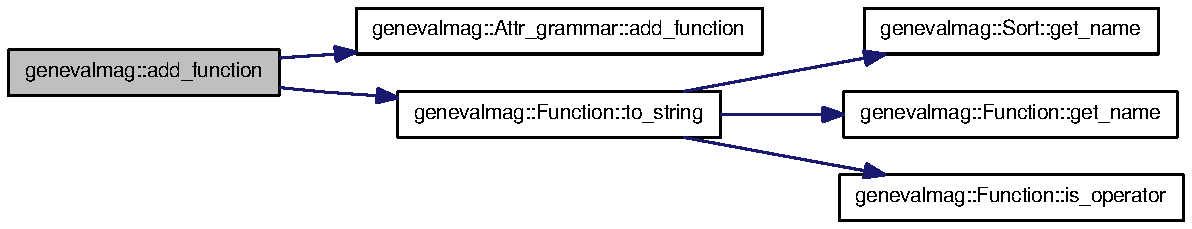
\includegraphics[width=304pt]{namespacegenevalmag_aff5e0f0cff477c34b63116d99dfbe9b0_cgraph}
\end{center}
\end{figure}




Here is the caller graph for this function:\nopagebreak
\begin{figure}[H]
\begin{center}
\leavevmode
\includegraphics[width=310pt]{namespacegenevalmag_aff5e0f0cff477c34b63116d99dfbe9b0_icgraph}
\end{center}
\end{figure}


\hypertarget{namespacegenevalmag_a5651e2842c6f77725d4c10f46655ead4}{
\index{genevalmag@{genevalmag}!add\_\-operator@{add\_\-operator}}
\index{add\_\-operator@{add\_\-operator}!genevalmag@{genevalmag}}
\subsubsection[{add\_\-operator}]{\setlength{\rightskip}{0pt plus 5cm}void genevalmag::add\_\-operator (const iterator\_\-t {\em str}, \/  const iterator\_\-t {\em end})}}
\label{namespacegenevalmag_a5651e2842c6f77725d4c10f46655ead4}
Methods and functions for parse Operator. 

Definition at line 135 of file Semantics\_\-actions.cpp.



References add\_\-function(), current\_\-func, IS\_\-OPERATOR(), and genevalmag::Function::set\_\-is\_\-operator().



Referenced by genevalmag::attritute\_\-grammar::definition$<$ ScannerT $>$::definition().



Here is the call graph for this function:\nopagebreak
\begin{figure}[H]
\begin{center}
\leavevmode
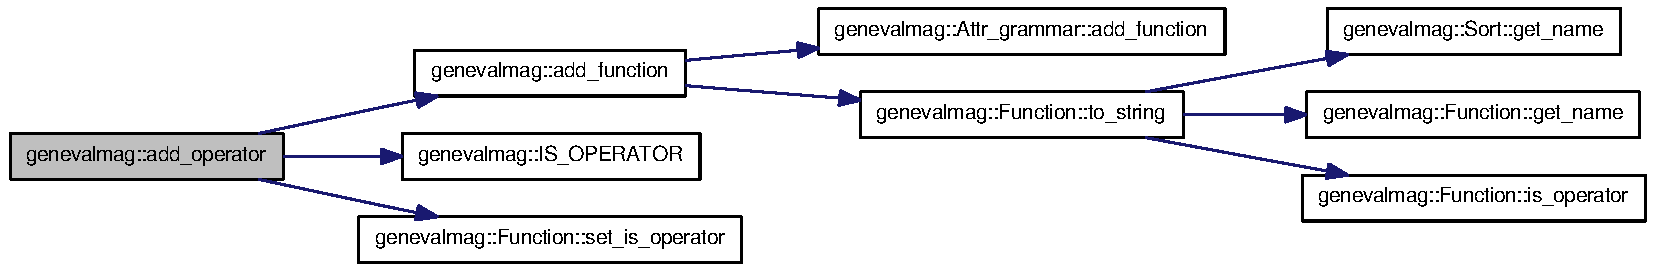
\includegraphics[width=415pt]{namespacegenevalmag_a5651e2842c6f77725d4c10f46655ead4_cgraph}
\end{center}
\end{figure}




Here is the caller graph for this function:\nopagebreak
\begin{figure}[H]
\begin{center}
\leavevmode
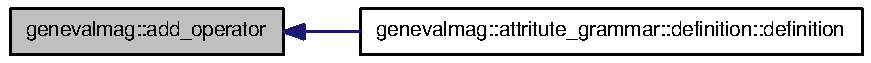
\includegraphics[width=227pt]{namespacegenevalmag_a5651e2842c6f77725d4c10f46655ead4_icgraph}
\end{center}
\end{figure}


\hypertarget{namespacegenevalmag_a9cb36d1a43794afa2b45c729c6c87170}{
\index{genevalmag@{genevalmag}!belong@{belong}}
\index{belong@{belong}!genevalmag@{genevalmag}}
\subsubsection[{belong}]{\setlength{\rightskip}{0pt plus 5cm}const bool genevalmag::belong (const Symbol \& {\em symb}, \/  const string \& {\em expr\_\-attrs})}}
\label{namespacegenevalmag_a9cb36d1a43794afa2b45c729c6c87170}
Interprets the expression of sets and returns true if the symbol belongs to that set. 

Definition at line 94 of file Attr\_\-grammar.cpp.



References genevalmag::Symbol::get\_\-name().



Referenced by genevalmag::Attr\_\-grammar::load\_\-attributes().



Here is the call graph for this function:\nopagebreak
\begin{figure}[H]
\begin{center}
\leavevmode
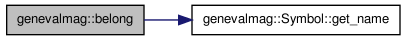
\includegraphics[width=170pt]{namespacegenevalmag_a9cb36d1a43794afa2b45c729c6c87170_cgraph}
\end{center}
\end{figure}




Here is the caller graph for this function:\nopagebreak
\begin{figure}[H]
\begin{center}
\leavevmode
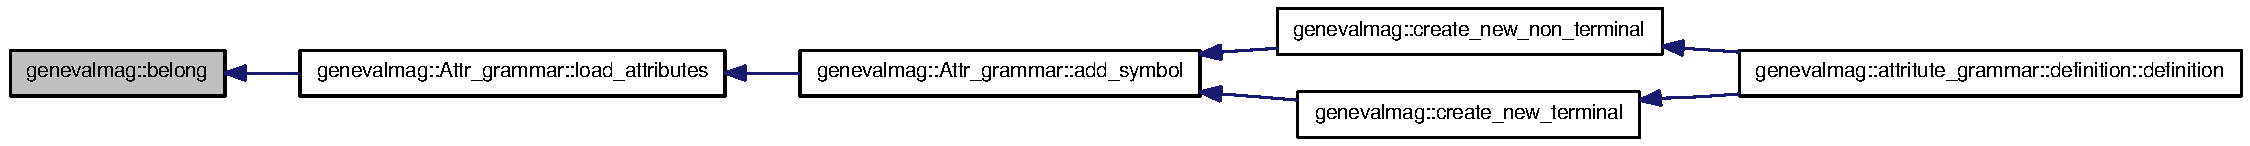
\includegraphics[width=420pt]{namespacegenevalmag_a9cb36d1a43794afa2b45c729c6c87170_icgraph}
\end{center}
\end{figure}


\hypertarget{namespacegenevalmag_ad52b23b8c38d8b9ef4c91820a512c963}{
\index{genevalmag@{genevalmag}!belong\_\-it@{belong\_\-it}}
\index{belong\_\-it@{belong\_\-it}!genevalmag@{genevalmag}}
\subsubsection[{belong\_\-it}]{\setlength{\rightskip}{0pt plus 5cm}bool genevalmag::belong\_\-it (const map$<$ Key\_\-plan, unsigned short $>$::const\_\-iterator {\em it}, \/  const vector$<$ map$<$ Key\_\-plan, unsigned short $>$::const\_\-iterator $>$ \& {\em vec})}}
\label{namespacegenevalmag_ad52b23b8c38d8b9ef4c91820a512c963}
Returns true if the iterator belongs to the vector passed as parameter. 

Definition at line 78 of file Builder\_\-visit\_\-sequences.cpp.



Referenced by genevalmag::Builder\_\-visit\_\-sequences::gen\_\-visit\_\-seq(), merge\_\-vec(), and merge\_\-vec\_\-without\_\-plan().



Here is the caller graph for this function:\nopagebreak
\begin{figure}[H]
\begin{center}
\leavevmode
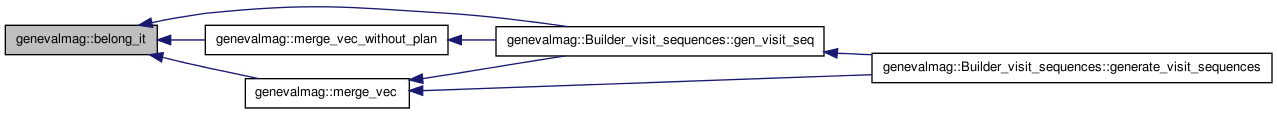
\includegraphics[width=420pt]{namespacegenevalmag_ad52b23b8c38d8b9ef4c91820a512c963_icgraph}
\end{center}
\end{figure}


\hypertarget{namespacegenevalmag_ad0ec9b7706a340d2e674f3b4859afa2d}{
\index{genevalmag@{genevalmag}!check\_\-eq\_\-defines\_\-it@{check\_\-eq\_\-defines\_\-it}}
\index{check\_\-eq\_\-defines\_\-it@{check\_\-eq\_\-defines\_\-it}!genevalmag@{genevalmag}}
\subsubsection[{check\_\-eq\_\-defines\_\-it}]{\setlength{\rightskip}{0pt plus 5cm}bool genevalmag::check\_\-eq\_\-defines\_\-it (const Symbol $\ast$ {\em symb}, \/  const int {\em index}, \/  const Attribute $\ast$ {\em attr}, \/  const map$<$ unsigned short, Equation $>$ {\em eqs})}}
\label{namespacegenevalmag_ad0ec9b7706a340d2e674f3b4859afa2d}
Checks if exist an equation that define the instance formed with the parameters. 

Definition at line 469 of file Semantics\_\-checks.cpp.



References genevalmag::Attribute::equals(), and genevalmag::Symbol::equals().



Referenced by genevalmag::Semantics\_\-checks::check\_\-well\_\-defined\_\-AG().



Here is the call graph for this function:\nopagebreak
\begin{figure}[H]
\begin{center}
\leavevmode
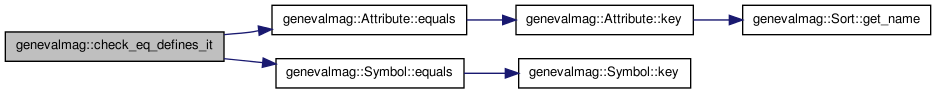
\includegraphics[width=369pt]{namespacegenevalmag_ad0ec9b7706a340d2e674f3b4859afa2d_cgraph}
\end{center}
\end{figure}




Here is the caller graph for this function:\nopagebreak
\begin{figure}[H]
\begin{center}
\leavevmode
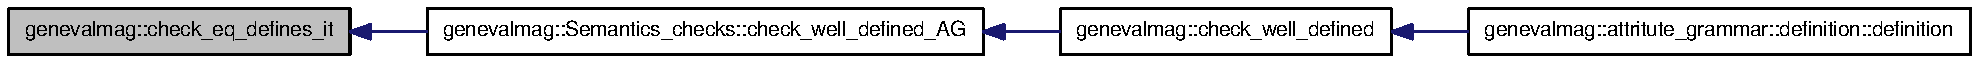
\includegraphics[width=420pt]{namespacegenevalmag_ad0ec9b7706a340d2e674f3b4859afa2d_icgraph}
\end{center}
\end{figure}


\hypertarget{namespacegenevalmag_a8d54caf5e5830cd48bf3265345928c3a}{
\index{genevalmag@{genevalmag}!check\_\-file\_\-exist@{check\_\-file\_\-exist}}
\index{check\_\-file\_\-exist@{check\_\-file\_\-exist}!genevalmag@{genevalmag}}
\subsubsection[{check\_\-file\_\-exist}]{\setlength{\rightskip}{0pt plus 5cm}bool genevalmag::check\_\-file\_\-exist (const string \& {\em strFilename})}}
\label{namespacegenevalmag_a8d54caf5e5830cd48bf3265345928c3a}


Definition at line 116 of file maggen.cpp.



Referenced by parse\_\-parameters().



Here is the caller graph for this function:\nopagebreak
\begin{figure}[H]
\begin{center}
\leavevmode
\includegraphics[width=227pt]{namespacegenevalmag_a8d54caf5e5830cd48bf3265345928c3a_icgraph}
\end{center}
\end{figure}


\hypertarget{namespacegenevalmag_a3bc888ab3b44c41a536427cf386f8c3d}{
\index{genevalmag@{genevalmag}!check\_\-name@{check\_\-name}}
\index{check\_\-name@{check\_\-name}!genevalmag@{genevalmag}}
\subsubsection[{check\_\-name}]{\setlength{\rightskip}{0pt plus 5cm}bool genevalmag::check\_\-name (const string \& {\em strFilename})}}
\label{namespacegenevalmag_a3bc888ab3b44c41a536427cf386f8c3d}


Definition at line 128 of file maggen.cpp.



Referenced by parse\_\-parameters().



Here is the caller graph for this function:\nopagebreak
\begin{figure}[H]
\begin{center}
\leavevmode
\includegraphics[width=219pt]{namespacegenevalmag_a3bc888ab3b44c41a536427cf386f8c3d_icgraph}
\end{center}
\end{figure}


\hypertarget{namespacegenevalmag_ac8f04dfdf39c964f9219cc5a7fb7197b}{
\index{genevalmag@{genevalmag}!check\_\-well\_\-defined@{check\_\-well\_\-defined}}
\index{check\_\-well\_\-defined@{check\_\-well\_\-defined}!genevalmag@{genevalmag}}
\subsubsection[{check\_\-well\_\-defined}]{\setlength{\rightskip}{0pt plus 5cm}void genevalmag::check\_\-well\_\-defined (const iterator\_\-t {\em str}, \/  const iterator\_\-t {\em end})}}
\label{namespacegenevalmag_ac8f04dfdf39c964f9219cc5a7fb7197b}


Definition at line 654 of file Semantics\_\-actions.cpp.



References attr\_\-grammar, genevalmag::Semantics\_\-checks::check\_\-all\_\-defined\_\-non\_\-terminal(), genevalmag::Semantics\_\-checks::check\_\-reachability(), genevalmag::Semantics\_\-checks::check\_\-well\_\-defined\_\-AG(), genevalmag::Attr\_\-grammar::get\_\-initial\_\-symb(), genevalmag::Attr\_\-grammar::get\_\-non\_\-terminal\_\-symbols(), genevalmag::Attr\_\-grammar::get\_\-rules(), and sem\_\-check.



Referenced by genevalmag::attritute\_\-grammar::definition$<$ ScannerT $>$::definition().



Here is the call graph for this function:\nopagebreak
\begin{figure}[H]
\begin{center}
\leavevmode
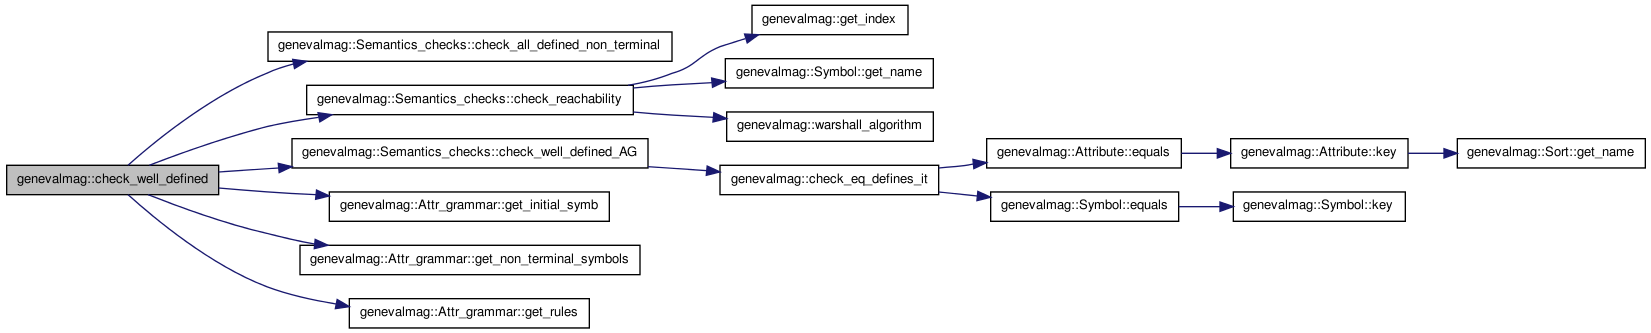
\includegraphics[width=420pt]{namespacegenevalmag_ac8f04dfdf39c964f9219cc5a7fb7197b_cgraph}
\end{center}
\end{figure}




Here is the caller graph for this function:\nopagebreak
\begin{figure}[H]
\begin{center}
\leavevmode
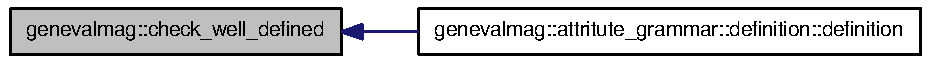
\includegraphics[width=241pt]{namespacegenevalmag_ac8f04dfdf39c964f9219cc5a7fb7197b_icgraph}
\end{center}
\end{figure}


\hypertarget{namespacegenevalmag_abd826b7a45bf0c29f45dc8f8c64c0805}{
\index{genevalmag@{genevalmag}!create\_\-abbreviated\_\-rule@{create\_\-abbreviated\_\-rule}}
\index{create\_\-abbreviated\_\-rule@{create\_\-abbreviated\_\-rule}!genevalmag@{genevalmag}}
\subsubsection[{create\_\-abbreviated\_\-rule}]{\setlength{\rightskip}{0pt plus 5cm}void genevalmag::create\_\-abbreviated\_\-rule (const iterator\_\-t {\em str}, \/  const iterator\_\-t {\em end})}}
\label{namespacegenevalmag_abd826b7a45bf0c29f45dc8f8c64c0805}


Definition at line 253 of file Semantics\_\-actions.cpp.



References current\_\-rule, genevalmag::Rule::get\_\-left\_\-symbol(), and genevalmag::Rule::set\_\-left\_\-symbol().



Referenced by genevalmag::attritute\_\-grammar::definition$<$ ScannerT $>$::definition().



Here is the call graph for this function:\nopagebreak
\begin{figure}[H]
\begin{center}
\leavevmode
\includegraphics[width=213pt]{namespacegenevalmag_abd826b7a45bf0c29f45dc8f8c64c0805_cgraph}
\end{center}
\end{figure}




Here is the caller graph for this function:\nopagebreak
\begin{figure}[H]
\begin{center}
\leavevmode
\includegraphics[width=250pt]{namespacegenevalmag_abd826b7a45bf0c29f45dc8f8c64c0805_icgraph}
\end{center}
\end{figure}


\hypertarget{namespacegenevalmag_a640285acc8edfe19e082795784dbbd51}{
\index{genevalmag@{genevalmag}!create\_\-attributes@{create\_\-attributes}}
\index{create\_\-attributes@{create\_\-attributes}!genevalmag@{genevalmag}}
\subsubsection[{create\_\-attributes}]{\setlength{\rightskip}{0pt plus 5cm}void genevalmag::create\_\-attributes (const iterator\_\-t {\em str}, \/  const iterator\_\-t {\em end})}}
\label{namespacegenevalmag_a640285acc8edfe19e082795784dbbd51}


Definition at line 204 of file Semantics\_\-actions.cpp.



References genevalmag::Attr\_\-grammar::add\_\-attribute(), attr\_\-grammar, genevalmag::decl\_\-attribute::d\_\-member\_\-symbol, genevalmag::decl\_\-attribute::d\_\-mod\_\-type, genevalmag::decl\_\-attribute::d\_\-names, genevalmag::decl\_\-attribute::d\_\-sort\_\-type, new\_\-attrs, genevalmag::Attr\_\-grammar::return\_\-sort(), genevalmag::Attribute::set\_\-member\_\-symbol(), genevalmag::Attribute::set\_\-mod\_\-type(), genevalmag::Attribute::set\_\-name(), and genevalmag::Attribute::set\_\-sort\_\-type().



Referenced by genevalmag::attritute\_\-grammar::definition$<$ ScannerT $>$::definition().



Here is the call graph for this function:\nopagebreak
\begin{figure}[H]
\begin{center}
\leavevmode
\includegraphics[width=325pt]{namespacegenevalmag_a640285acc8edfe19e082795784dbbd51_cgraph}
\end{center}
\end{figure}




Here is the caller graph for this function:\nopagebreak
\begin{figure}[H]
\begin{center}
\leavevmode
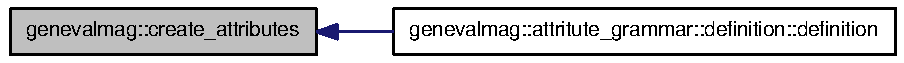
\includegraphics[width=235pt]{namespacegenevalmag_a640285acc8edfe19e082795784dbbd51_icgraph}
\end{center}
\end{figure}


\hypertarget{namespacegenevalmag_ab6467a68d84550ca5d16d15c247499f4}{
\index{genevalmag@{genevalmag}!create\_\-bool@{create\_\-bool}}
\index{create\_\-bool@{create\_\-bool}!genevalmag@{genevalmag}}
\subsubsection[{create\_\-bool}]{\setlength{\rightskip}{0pt plus 5cm}void genevalmag::create\_\-bool (const iterator\_\-t {\em str}, \/  const iterator\_\-t {\em end})}}
\label{namespacegenevalmag_ab6467a68d84550ca5d16d15c247499f4}


Definition at line 361 of file Semantics\_\-actions.cpp.



References current\_\-literal, k\_\-bool, genevalmag::Expr\_\-literal::set\_\-type(), genevalmag::Expression::set\_\-type\_\-synthetized(), and genevalmag::Expr\_\-literal::set\_\-value().



Referenced by genevalmag::attritute\_\-grammar::definition$<$ ScannerT $>$::definition().



Here is the call graph for this function:\nopagebreak
\begin{figure}[H]
\begin{center}
\leavevmode
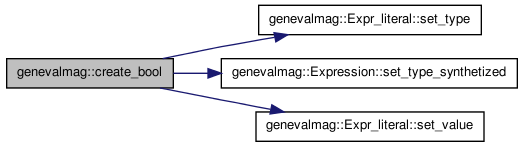
\includegraphics[width=214pt]{namespacegenevalmag_ab6467a68d84550ca5d16d15c247499f4_cgraph}
\end{center}
\end{figure}




Here is the caller graph for this function:\nopagebreak
\begin{figure}[H]
\begin{center}
\leavevmode
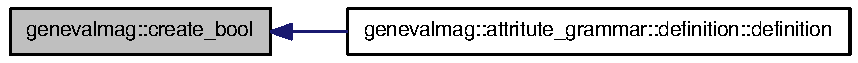
\includegraphics[width=224pt]{namespacegenevalmag_ab6467a68d84550ca5d16d15c247499f4_icgraph}
\end{center}
\end{figure}


\hypertarget{namespacegenevalmag_ac0759c1555b62ec188a704ee700aac2a}{
\index{genevalmag@{genevalmag}!create\_\-equation@{create\_\-equation}}
\index{create\_\-equation@{create\_\-equation}!genevalmag@{genevalmag}}
\subsubsection[{create\_\-equation}]{\setlength{\rightskip}{0pt plus 5cm}void genevalmag::create\_\-equation (const iterator\_\-t {\em str}, \/  const iterator\_\-t {\em end})}}
\label{namespacegenevalmag_ac0759c1555b62ec188a704ee700aac2a}


Definition at line 385 of file Semantics\_\-actions.cpp.



References current\_\-eq, current\_\-instance, and genevalmag::Equation::set\_\-l\_\-value().



Referenced by genevalmag::attritute\_\-grammar::definition$<$ ScannerT $>$::definition().



Here is the call graph for this function:\nopagebreak
\begin{figure}[H]
\begin{center}
\leavevmode
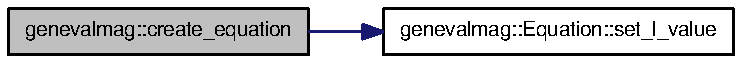
\includegraphics[width=196pt]{namespacegenevalmag_ac0759c1555b62ec188a704ee700aac2a_cgraph}
\end{center}
\end{figure}




Here is the caller graph for this function:\nopagebreak
\begin{figure}[H]
\begin{center}
\leavevmode
\includegraphics[width=233pt]{namespacegenevalmag_ac0759c1555b62ec188a704ee700aac2a_icgraph}
\end{center}
\end{figure}


\hypertarget{namespacegenevalmag_a2f41a8b96eb7d5bdca16a4924dcd020f}{
\index{genevalmag@{genevalmag}!create\_\-func\_\-node@{create\_\-func\_\-node}}
\index{create\_\-func\_\-node@{create\_\-func\_\-node}!genevalmag@{genevalmag}}
\subsubsection[{create\_\-func\_\-node}]{\setlength{\rightskip}{0pt plus 5cm}void genevalmag::create\_\-func\_\-node (const iterator\_\-t {\em str}, \/  const iterator\_\-t {\em end})}}
\label{namespacegenevalmag_a2f41a8b96eb7d5bdca16a4924dcd020f}


Definition at line 459 of file Semantics\_\-actions.cpp.



References current\_\-ast\_\-function, current\_\-func, genevalmag::Semantics\_\-checks::get\_\-index\_\-syntax\_\-order(), genevalmag::Semantics\_\-checks::get\_\-precedence\_\-level(), genevalmag::Semantics\_\-checks::increment\_\-index\_\-syntax\_\-order(), sem\_\-check, genevalmag::Expr\_\-function::set\_\-function(), genevalmag::Expr\_\-function::set\_\-precedence\_\-level(), genevalmag::Expr\_\-function::set\_\-syntax\_\-order(), and stack\_\-inner\_\-node.



Referenced by genevalmag::attritute\_\-grammar::definition$<$ ScannerT $>$::definition().



Here is the call graph for this function:\nopagebreak
\begin{figure}[H]
\begin{center}
\leavevmode
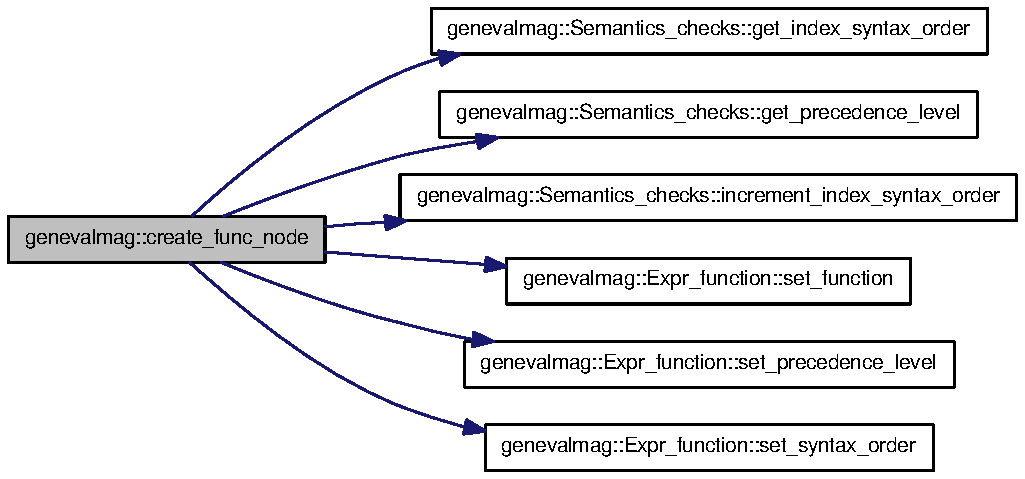
\includegraphics[width=264pt]{namespacegenevalmag_a2f41a8b96eb7d5bdca16a4924dcd020f_cgraph}
\end{center}
\end{figure}




Here is the caller graph for this function:\nopagebreak
\begin{figure}[H]
\begin{center}
\leavevmode
\includegraphics[width=237pt]{namespacegenevalmag_a2f41a8b96eb7d5bdca16a4924dcd020f_icgraph}
\end{center}
\end{figure}


\hypertarget{namespacegenevalmag_a166358b221cbf34ec512b137326d6c44}{
\index{genevalmag@{genevalmag}!create\_\-function@{create\_\-function}}
\index{create\_\-function@{create\_\-function}!genevalmag@{genevalmag}}
\subsubsection[{create\_\-function}]{\setlength{\rightskip}{0pt plus 5cm}void genevalmag::create\_\-function (const iterator\_\-t {\em str}, \/  const iterator\_\-t {\em end})}}
\label{namespacegenevalmag_a166358b221cbf34ec512b137326d6c44}


Definition at line 373 of file Semantics\_\-actions.cpp.



References current\_\-func, and save\_\-name\_\-func().



Referenced by create\_\-operator(), and genevalmag::attritute\_\-grammar::definition$<$ ScannerT $>$::definition().



Here is the call graph for this function:\nopagebreak
\begin{figure}[H]
\begin{center}
\leavevmode
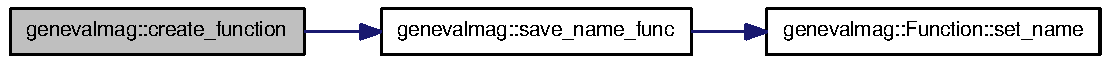
\includegraphics[width=284pt]{namespacegenevalmag_a166358b221cbf34ec512b137326d6c44_cgraph}
\end{center}
\end{figure}




Here is the caller graph for this function:\nopagebreak
\begin{figure}[H]
\begin{center}
\leavevmode
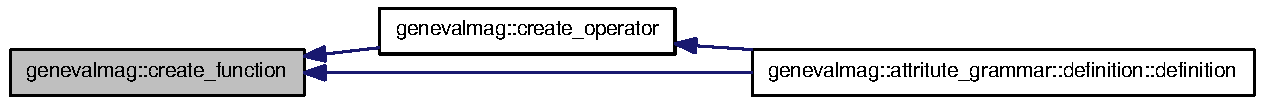
\includegraphics[width=321pt]{namespacegenevalmag_a166358b221cbf34ec512b137326d6c44_icgraph}
\end{center}
\end{figure}


\hypertarget{namespacegenevalmag_a61de26b3fdfcf0998039df573a3ec6f0}{
\index{genevalmag@{genevalmag}!create\_\-instance@{create\_\-instance}}
\index{create\_\-instance@{create\_\-instance}!genevalmag@{genevalmag}}
\subsubsection[{create\_\-instance}]{\setlength{\rightskip}{0pt plus 5cm}void genevalmag::create\_\-instance (const iterator\_\-t {\em str}, \/  const iterator\_\-t {\em end})}}
\label{namespacegenevalmag_a61de26b3fdfcf0998039df573a3ec6f0}
Methods and functions for parse \hyperlink{classgenevalmag_1_1Equation}{Equation} class of \hyperlink{classgenevalmag_1_1Rule}{Rule}. 

Definition at line 268 of file Semantics\_\-actions.cpp.



References attr\_\-grammar, genevalmag::Rule::belongs\_\-non\_\-terminal(), utilities::cleaning\_\-tabs(), current\_\-instance, current\_\-rule, genevalmag::Attr\_\-grammar::get\_\-symbol(), genevalmag::Expr\_\-instance::set\_\-symb(), and genevalmag::Rule::to\_\-string\_\-not\_\-eqs().



Referenced by genevalmag::attritute\_\-grammar::definition$<$ ScannerT $>$::definition().



Here is the call graph for this function:\nopagebreak
\begin{figure}[H]
\begin{center}
\leavevmode
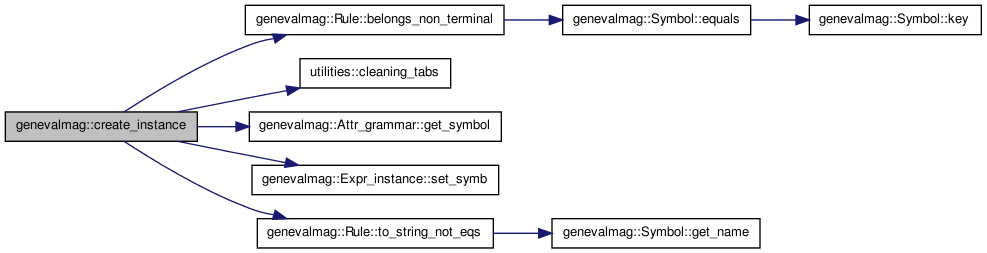
\includegraphics[width=388pt]{namespacegenevalmag_a61de26b3fdfcf0998039df573a3ec6f0_cgraph}
\end{center}
\end{figure}




Here is the caller graph for this function:\nopagebreak
\begin{figure}[H]
\begin{center}
\leavevmode
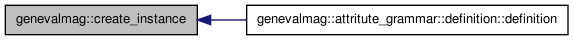
\includegraphics[width=233pt]{namespacegenevalmag_a61de26b3fdfcf0998039df573a3ec6f0_icgraph}
\end{center}
\end{figure}


\hypertarget{namespacegenevalmag_a931db9fc9546a03ac92ae77ca4ad9f21}{
\index{genevalmag@{genevalmag}!create\_\-instance\_\-node@{create\_\-instance\_\-node}}
\index{create\_\-instance\_\-node@{create\_\-instance\_\-node}!genevalmag@{genevalmag}}
\subsubsection[{create\_\-instance\_\-node}]{\setlength{\rightskip}{0pt plus 5cm}void genevalmag::create\_\-instance\_\-node (const iterator\_\-t {\em str}, \/  const iterator\_\-t {\em end})}}
\label{namespacegenevalmag_a931db9fc9546a03ac92ae77ca4ad9f21}


Definition at line 450 of file Semantics\_\-actions.cpp.



References current\_\-instance, genevalmag::Expr\_\-instance::get\_\-attr(), genevalmag::Sort::get\_\-name(), genevalmag::Attribute::get\_\-sort\_\-type(), genevalmag::Expression::set\_\-type\_\-synthetized(), and stack\_\-node.



Referenced by genevalmag::attritute\_\-grammar::definition$<$ ScannerT $>$::definition().



Here is the call graph for this function:\nopagebreak
\begin{figure}[H]
\begin{center}
\leavevmode
\includegraphics[width=236pt]{namespacegenevalmag_a931db9fc9546a03ac92ae77ca4ad9f21_cgraph}
\end{center}
\end{figure}




Here is the caller graph for this function:\nopagebreak
\begin{figure}[H]
\begin{center}
\leavevmode
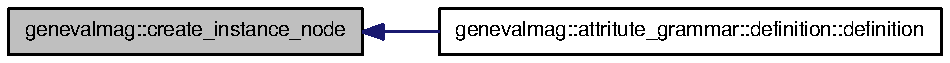
\includegraphics[width=246pt]{namespacegenevalmag_a931db9fc9546a03ac92ae77ca4ad9f21_icgraph}
\end{center}
\end{figure}


\hypertarget{namespacegenevalmag_a48bc87a884f21e2f39a19b6ef43bedf9}{
\index{genevalmag@{genevalmag}!create\_\-lit\_\-ch@{create\_\-lit\_\-ch}}
\index{create\_\-lit\_\-ch@{create\_\-lit\_\-ch}!genevalmag@{genevalmag}}
\subsubsection[{create\_\-lit\_\-ch}]{\setlength{\rightskip}{0pt plus 5cm}void genevalmag::create\_\-lit\_\-ch (const iterator\_\-t {\em ch}, \/  const iterator\_\-t {\em end})}}
\label{namespacegenevalmag_a48bc87a884f21e2f39a19b6ef43bedf9}


Definition at line 333 of file Semantics\_\-actions.cpp.



References current\_\-literal, k\_\-char, genevalmag::Expr\_\-literal::set\_\-type(), genevalmag::Expression::set\_\-type\_\-synthetized(), and genevalmag::Expr\_\-literal::set\_\-value().



Referenced by genevalmag::attritute\_\-grammar::definition$<$ ScannerT $>$::definition().



Here is the call graph for this function:\nopagebreak
\begin{figure}[H]
\begin{center}
\leavevmode
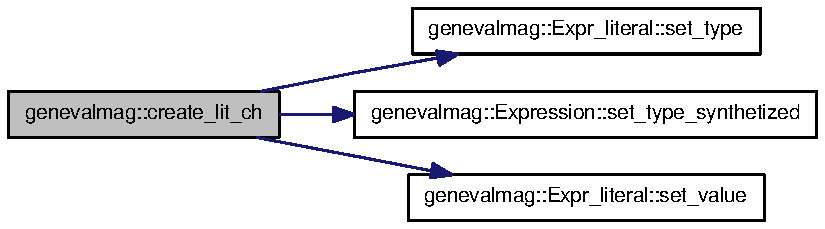
\includegraphics[width=216pt]{namespacegenevalmag_a48bc87a884f21e2f39a19b6ef43bedf9_cgraph}
\end{center}
\end{figure}




Here is the caller graph for this function:\nopagebreak
\begin{figure}[H]
\begin{center}
\leavevmode
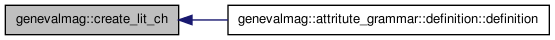
\includegraphics[width=226pt]{namespacegenevalmag_a48bc87a884f21e2f39a19b6ef43bedf9_icgraph}
\end{center}
\end{figure}


\hypertarget{namespacegenevalmag_a380b107e4dbce952517d6aac470e7ce7}{
\index{genevalmag@{genevalmag}!create\_\-lit\_\-number@{create\_\-lit\_\-number}}
\index{create\_\-lit\_\-number@{create\_\-lit\_\-number}!genevalmag@{genevalmag}}
\subsubsection[{create\_\-lit\_\-number}]{\setlength{\rightskip}{0pt plus 5cm}void genevalmag::create\_\-lit\_\-number (const iterator\_\-t {\em str}, \/  const iterator\_\-t {\em end})}}
\label{namespacegenevalmag_a380b107e4dbce952517d6aac470e7ce7}


Definition at line 309 of file Semantics\_\-actions.cpp.



References current\_\-literal, k\_\-float, k\_\-int, genevalmag::Expr\_\-literal::set\_\-type(), genevalmag::Expression::set\_\-type\_\-synthetized(), and genevalmag::Expr\_\-literal::set\_\-value().



Referenced by genevalmag::attritute\_\-grammar::definition$<$ ScannerT $>$::definition().



Here is the call graph for this function:\nopagebreak
\begin{figure}[H]
\begin{center}
\leavevmode
\includegraphics[width=227pt]{namespacegenevalmag_a380b107e4dbce952517d6aac470e7ce7_cgraph}
\end{center}
\end{figure}




Here is the caller graph for this function:\nopagebreak
\begin{figure}[H]
\begin{center}
\leavevmode
\includegraphics[width=237pt]{namespacegenevalmag_a380b107e4dbce952517d6aac470e7ce7_icgraph}
\end{center}
\end{figure}


\hypertarget{namespacegenevalmag_a474728745db913b81459a7267bb28222}{
\index{genevalmag@{genevalmag}!create\_\-lit\_\-str@{create\_\-lit\_\-str}}
\index{create\_\-lit\_\-str@{create\_\-lit\_\-str}!genevalmag@{genevalmag}}
\subsubsection[{create\_\-lit\_\-str}]{\setlength{\rightskip}{0pt plus 5cm}void genevalmag::create\_\-lit\_\-str (const iterator\_\-t {\em str}, \/  const iterator\_\-t {\em end})}}
\label{namespacegenevalmag_a474728745db913b81459a7267bb28222}


Definition at line 347 of file Semantics\_\-actions.cpp.



References current\_\-literal, k\_\-string, genevalmag::Expr\_\-literal::set\_\-type(), genevalmag::Expression::set\_\-type\_\-synthetized(), and genevalmag::Expr\_\-literal::set\_\-value().



Referenced by genevalmag::attritute\_\-grammar::definition$<$ ScannerT $>$::definition().



Here is the call graph for this function:\nopagebreak
\begin{figure}[H]
\begin{center}
\leavevmode
\includegraphics[width=217pt]{namespacegenevalmag_a474728745db913b81459a7267bb28222_cgraph}
\end{center}
\end{figure}




Here is the caller graph for this function:\nopagebreak
\begin{figure}[H]
\begin{center}
\leavevmode
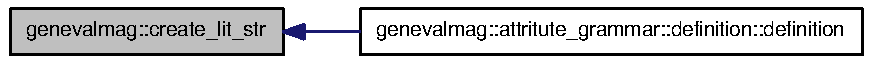
\includegraphics[width=227pt]{namespacegenevalmag_a474728745db913b81459a7267bb28222_icgraph}
\end{center}
\end{figure}


\hypertarget{namespacegenevalmag_a5acc69c06c112cad864e048a095396c5}{
\index{genevalmag@{genevalmag}!create\_\-literal\_\-node@{create\_\-literal\_\-node}}
\index{create\_\-literal\_\-node@{create\_\-literal\_\-node}!genevalmag@{genevalmag}}
\subsubsection[{create\_\-literal\_\-node}]{\setlength{\rightskip}{0pt plus 5cm}void genevalmag::create\_\-literal\_\-node (const iterator\_\-t {\em str}, \/  const iterator\_\-t {\em end})}}
\label{namespacegenevalmag_a5acc69c06c112cad864e048a095396c5}
Creation expression nodes. 

Definition at line 443 of file Semantics\_\-actions.cpp.



References current\_\-literal, and stack\_\-node.



Referenced by genevalmag::attritute\_\-grammar::definition$<$ ScannerT $>$::definition().



Here is the caller graph for this function:\nopagebreak
\begin{figure}[H]
\begin{center}
\leavevmode
\includegraphics[width=239pt]{namespacegenevalmag_a5acc69c06c112cad864e048a095396c5_icgraph}
\end{center}
\end{figure}


\hypertarget{namespacegenevalmag_a6d8584e0b692b4a20384e0742b22630a}{
\index{genevalmag@{genevalmag}!create\_\-new\_\-non\_\-terminal@{create\_\-new\_\-non\_\-terminal}}
\index{create\_\-new\_\-non\_\-terminal@{create\_\-new\_\-non\_\-terminal}!genevalmag@{genevalmag}}
\subsubsection[{create\_\-new\_\-non\_\-terminal}]{\setlength{\rightskip}{0pt plus 5cm}void genevalmag::create\_\-new\_\-non\_\-terminal (const iterator\_\-t {\em str}, \/  const iterator\_\-t {\em end})}}
\label{namespacegenevalmag_a6d8584e0b692b4a20384e0742b22630a}
Methods and functions for parse \hyperlink{classgenevalmag_1_1Symbol}{Symbol} class. 

Definition at line 223 of file Semantics\_\-actions.cpp.



References genevalmag::Attr\_\-grammar::add\_\-symbol(), attr\_\-grammar, and k\_\-non\_\-terminal.



Referenced by genevalmag::attritute\_\-grammar::definition$<$ ScannerT $>$::definition().



Here is the call graph for this function:\nopagebreak
\begin{figure}[H]
\begin{center}
\leavevmode
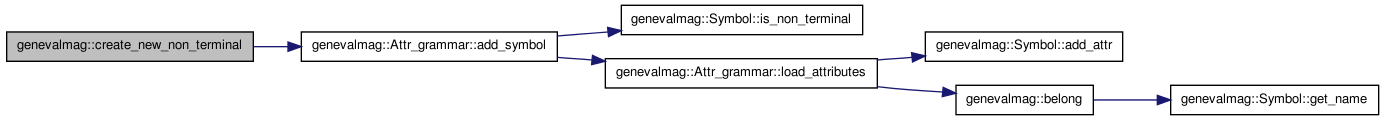
\includegraphics[width=420pt]{namespacegenevalmag_a6d8584e0b692b4a20384e0742b22630a_cgraph}
\end{center}
\end{figure}




Here is the caller graph for this function:\nopagebreak
\begin{figure}[H]
\begin{center}
\leavevmode
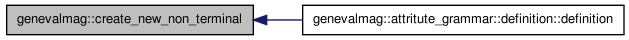
\includegraphics[width=254pt]{namespacegenevalmag_a6d8584e0b692b4a20384e0742b22630a_icgraph}
\end{center}
\end{figure}


\hypertarget{namespacegenevalmag_a3ab01d2c2dc547707d49394c59211460}{
\index{genevalmag@{genevalmag}!create\_\-new\_\-terminal@{create\_\-new\_\-terminal}}
\index{create\_\-new\_\-terminal@{create\_\-new\_\-terminal}!genevalmag@{genevalmag}}
\subsubsection[{create\_\-new\_\-terminal}]{\setlength{\rightskip}{0pt plus 5cm}void genevalmag::create\_\-new\_\-terminal (const iterator\_\-t {\em str}, \/  const iterator\_\-t {\em end})}}
\label{namespacegenevalmag_a3ab01d2c2dc547707d49394c59211460}


Definition at line 230 of file Semantics\_\-actions.cpp.



References genevalmag::Attr\_\-grammar::add\_\-symbol(), attr\_\-grammar, and k\_\-terminal.



Referenced by genevalmag::attritute\_\-grammar::definition$<$ ScannerT $>$::definition().



Here is the call graph for this function:\nopagebreak
\begin{figure}[H]
\begin{center}
\leavevmode
\includegraphics[width=420pt]{namespacegenevalmag_a3ab01d2c2dc547707d49394c59211460_cgraph}
\end{center}
\end{figure}




Here is the caller graph for this function:\nopagebreak
\begin{figure}[H]
\begin{center}
\leavevmode
\includegraphics[width=243pt]{namespacegenevalmag_a3ab01d2c2dc547707d49394c59211460_icgraph}
\end{center}
\end{figure}


\hypertarget{namespacegenevalmag_afa1b5eab4ae88dcc8cdea82c8a94042e}{
\index{genevalmag@{genevalmag}!create\_\-operator@{create\_\-operator}}
\index{create\_\-operator@{create\_\-operator}!genevalmag@{genevalmag}}
\subsubsection[{create\_\-operator}]{\setlength{\rightskip}{0pt plus 5cm}void genevalmag::create\_\-operator (const iterator\_\-t {\em str}, \/  const iterator\_\-t {\em end})}}
\label{namespacegenevalmag_afa1b5eab4ae88dcc8cdea82c8a94042e}


Definition at line 379 of file Semantics\_\-actions.cpp.



References create\_\-function(), current\_\-func, IS\_\-OPERATOR(), and genevalmag::Function::set\_\-is\_\-operator().



Referenced by genevalmag::attritute\_\-grammar::definition$<$ ScannerT $>$::definition().



Here is the call graph for this function:\nopagebreak
\begin{figure}[H]
\begin{center}
\leavevmode
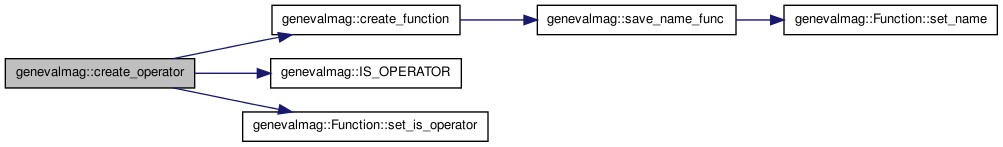
\includegraphics[width=394pt]{namespacegenevalmag_afa1b5eab4ae88dcc8cdea82c8a94042e_cgraph}
\end{center}
\end{figure}




Here is the caller graph for this function:\nopagebreak
\begin{figure}[H]
\begin{center}
\leavevmode
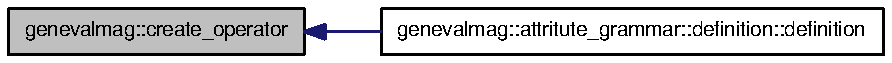
\includegraphics[width=232pt]{namespacegenevalmag_afa1b5eab4ae88dcc8cdea82c8a94042e_icgraph}
\end{center}
\end{figure}


\hypertarget{namespacegenevalmag_abf7e87f4c01eacdac90dd0875d9e1f0a}{
\index{genevalmag@{genevalmag}!create\_\-root\_\-function\_\-node@{create\_\-root\_\-function\_\-node}}
\index{create\_\-root\_\-function\_\-node@{create\_\-root\_\-function\_\-node}!genevalmag@{genevalmag}}
\subsubsection[{create\_\-root\_\-function\_\-node}]{\setlength{\rightskip}{0pt plus 5cm}void genevalmag::create\_\-root\_\-function\_\-node (const iterator\_\-t {\em str}, \/  const iterator\_\-t {\em end})}}
\label{namespacegenevalmag_abf7e87f4c01eacdac90dd0875d9e1f0a}


Definition at line 524 of file Semantics\_\-actions.cpp.



References attr\_\-grammar, genevalmag::Attr\_\-grammar::get\_\-function(), stack\_\-inner\_\-node, and stack\_\-node.



Referenced by genevalmag::attritute\_\-grammar::definition$<$ ScannerT $>$::definition().



Here is the call graph for this function:\nopagebreak
\begin{figure}[H]
\begin{center}
\leavevmode
\includegraphics[width=232pt]{namespacegenevalmag_abf7e87f4c01eacdac90dd0875d9e1f0a_cgraph}
\end{center}
\end{figure}




Here is the caller graph for this function:\nopagebreak
\begin{figure}[H]
\begin{center}
\leavevmode
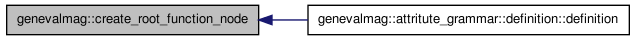
\includegraphics[width=256pt]{namespacegenevalmag_abf7e87f4c01eacdac90dd0875d9e1f0a_icgraph}
\end{center}
\end{figure}


\hypertarget{namespacegenevalmag_a2a5aaaff7c3b3b8efc446903121a62c6}{
\index{genevalmag@{genevalmag}!create\_\-root\_\-infix\_\-node@{create\_\-root\_\-infix\_\-node}}
\index{create\_\-root\_\-infix\_\-node@{create\_\-root\_\-infix\_\-node}!genevalmag@{genevalmag}}
\subsubsection[{create\_\-root\_\-infix\_\-node}]{\setlength{\rightskip}{0pt plus 5cm}void genevalmag::create\_\-root\_\-infix\_\-node (const iterator\_\-t {\em str}, \/  const iterator\_\-t {\em end})}}
\label{namespacegenevalmag_a2a5aaaff7c3b3b8efc446903121a62c6}


Definition at line 477 of file Semantics\_\-actions.cpp.



References attr\_\-grammar, genevalmag::Semantics\_\-checks::correct\_\-precedence(), genevalmag::Attr\_\-grammar::get\_\-function(), sem\_\-check, stack\_\-inner\_\-node, and stack\_\-node.



Referenced by genevalmag::attritute\_\-grammar::definition$<$ ScannerT $>$::definition().



Here is the call graph for this function:\nopagebreak
\begin{figure}[H]
\begin{center}
\leavevmode
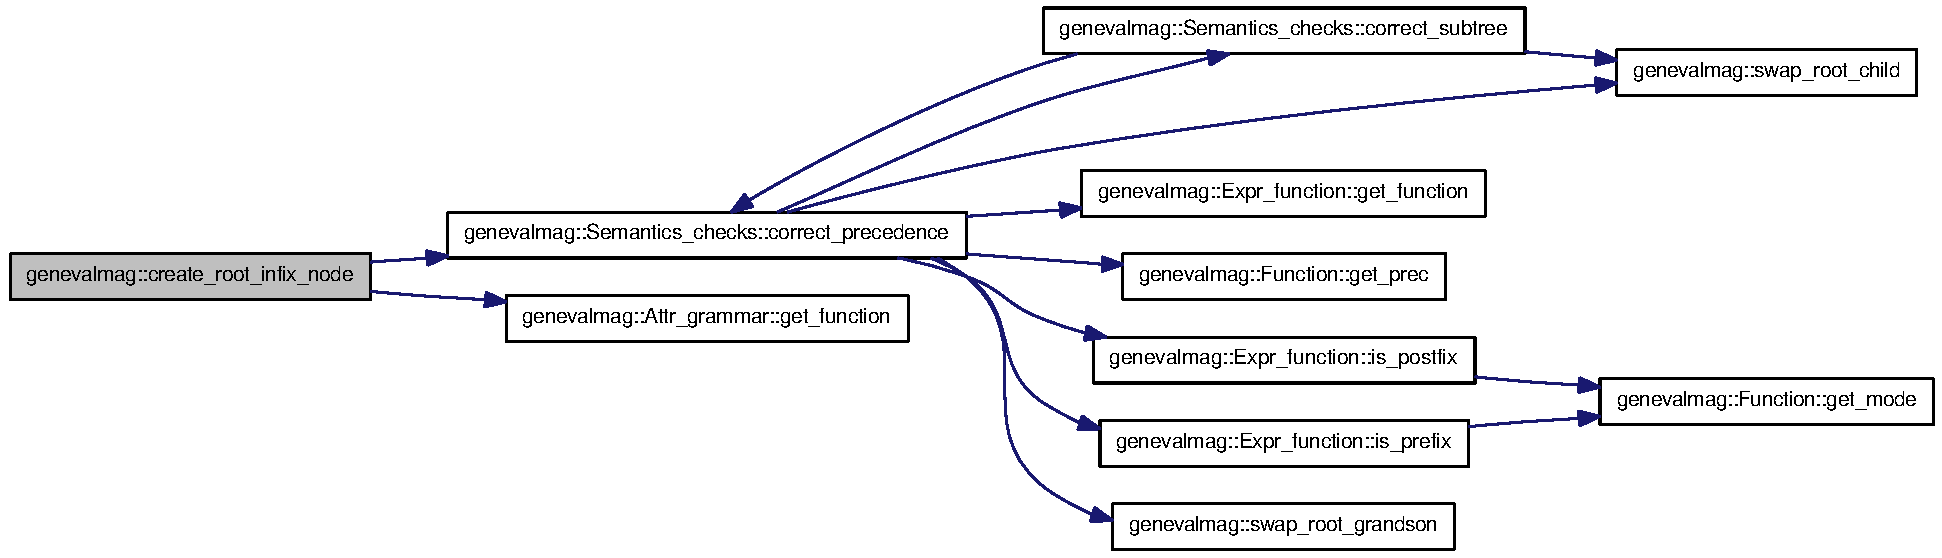
\includegraphics[width=420pt]{namespacegenevalmag_a2a5aaaff7c3b3b8efc446903121a62c6_cgraph}
\end{center}
\end{figure}




Here is the caller graph for this function:\nopagebreak
\begin{figure}[H]
\begin{center}
\leavevmode
\includegraphics[width=248pt]{namespacegenevalmag_a2a5aaaff7c3b3b8efc446903121a62c6_icgraph}
\end{center}
\end{figure}


\hypertarget{namespacegenevalmag_ad2e6e0ea9f03843a2adb23ea4c43453f}{
\index{genevalmag@{genevalmag}!create\_\-root\_\-postfix\_\-node@{create\_\-root\_\-postfix\_\-node}}
\index{create\_\-root\_\-postfix\_\-node@{create\_\-root\_\-postfix\_\-node}!genevalmag@{genevalmag}}
\subsubsection[{create\_\-root\_\-postfix\_\-node}]{\setlength{\rightskip}{0pt plus 5cm}void genevalmag::create\_\-root\_\-postfix\_\-node (const iterator\_\-t {\em str}, \/  const iterator\_\-t {\em end})}}
\label{namespacegenevalmag_ad2e6e0ea9f03843a2adb23ea4c43453f}


Definition at line 574 of file Semantics\_\-actions.cpp.



References attr\_\-grammar, genevalmag::Semantics\_\-checks::correct\_\-precedence(), genevalmag::Attr\_\-grammar::get\_\-function(), sem\_\-check, stack\_\-inner\_\-node, and stack\_\-node.



Referenced by genevalmag::attritute\_\-grammar::definition$<$ ScannerT $>$::definition().



Here is the call graph for this function:\nopagebreak
\begin{figure}[H]
\begin{center}
\leavevmode
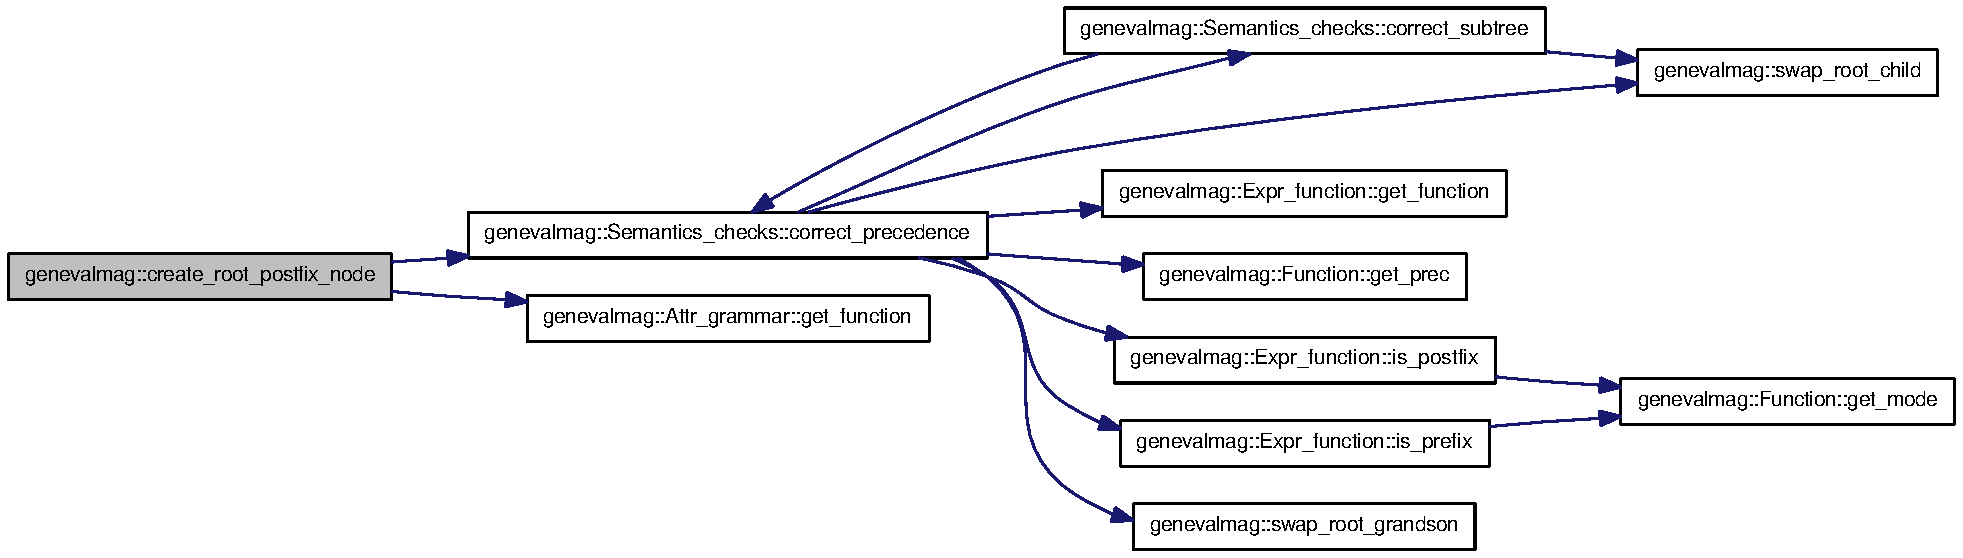
\includegraphics[width=420pt]{namespacegenevalmag_ad2e6e0ea9f03843a2adb23ea4c43453f_cgraph}
\end{center}
\end{figure}




Here is the caller graph for this function:\nopagebreak
\begin{figure}[H]
\begin{center}
\leavevmode
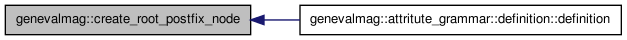
\includegraphics[width=253pt]{namespacegenevalmag_ad2e6e0ea9f03843a2adb23ea4c43453f_icgraph}
\end{center}
\end{figure}


\hypertarget{namespacegenevalmag_a2947fff1246a0fbe137217896a658a5b}{
\index{genevalmag@{genevalmag}!create\_\-root\_\-prefix\_\-node@{create\_\-root\_\-prefix\_\-node}}
\index{create\_\-root\_\-prefix\_\-node@{create\_\-root\_\-prefix\_\-node}!genevalmag@{genevalmag}}
\subsubsection[{create\_\-root\_\-prefix\_\-node}]{\setlength{\rightskip}{0pt plus 5cm}void genevalmag::create\_\-root\_\-prefix\_\-node (const iterator\_\-t {\em str}, \/  const iterator\_\-t {\em end})}}
\label{namespacegenevalmag_a2947fff1246a0fbe137217896a658a5b}


Definition at line 614 of file Semantics\_\-actions.cpp.



References attr\_\-grammar, genevalmag::Semantics\_\-checks::correct\_\-precedence(), genevalmag::Attr\_\-grammar::get\_\-function(), sem\_\-check, stack\_\-inner\_\-node, and stack\_\-node.



Referenced by genevalmag::attritute\_\-grammar::definition$<$ ScannerT $>$::definition().



Here is the call graph for this function:\nopagebreak
\begin{figure}[H]
\begin{center}
\leavevmode
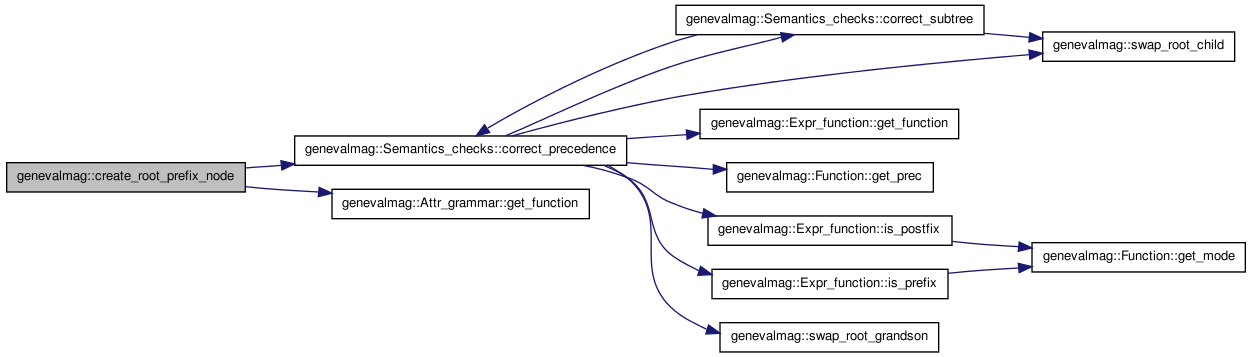
\includegraphics[width=420pt]{namespacegenevalmag_a2947fff1246a0fbe137217896a658a5b_cgraph}
\end{center}
\end{figure}




Here is the caller graph for this function:\nopagebreak
\begin{figure}[H]
\begin{center}
\leavevmode
\includegraphics[width=251pt]{namespacegenevalmag_a2947fff1246a0fbe137217896a658a5b_icgraph}
\end{center}
\end{figure}


\hypertarget{namespacegenevalmag_a38a9e6cd331b8e5caad524d12229d71e}{
\index{genevalmag@{genevalmag}!create\_\-rule@{create\_\-rule}}
\index{create\_\-rule@{create\_\-rule}!genevalmag@{genevalmag}}
\subsubsection[{create\_\-rule}]{\setlength{\rightskip}{0pt plus 5cm}void genevalmag::create\_\-rule (const iterator\_\-t {\em str}, \/  const iterator\_\-t {\em end})}}
\label{namespacegenevalmag_a38a9e6cd331b8e5caad524d12229d71e}
Methods and functions for parse \hyperlink{classgenevalmag_1_1Rule}{Rule} class. 

Definition at line 240 of file Semantics\_\-actions.cpp.



References attr\_\-grammar, current\_\-rule, genevalmag::Attr\_\-grammar::get\_\-symbol(), and genevalmag::Rule::set\_\-left\_\-symbol().



Referenced by genevalmag::attritute\_\-grammar::definition$<$ ScannerT $>$::definition().



Here is the call graph for this function:\nopagebreak
\begin{figure}[H]
\begin{center}
\leavevmode
\includegraphics[width=197pt]{namespacegenevalmag_a38a9e6cd331b8e5caad524d12229d71e_cgraph}
\end{center}
\end{figure}




Here is the caller graph for this function:\nopagebreak
\begin{figure}[H]
\begin{center}
\leavevmode
\includegraphics[width=223pt]{namespacegenevalmag_a38a9e6cd331b8e5caad524d12229d71e_icgraph}
\end{center}
\end{figure}


\hypertarget{namespacegenevalmag_a8fe47e97e9f000f1eb35ee9e86b2a5c0}{
\index{genevalmag@{genevalmag}!create\_\-sort@{create\_\-sort}}
\index{create\_\-sort@{create\_\-sort}!genevalmag@{genevalmag}}
\subsubsection[{create\_\-sort}]{\setlength{\rightskip}{0pt plus 5cm}void genevalmag::create\_\-sort (const iterator\_\-t {\em str}, \/  const iterator\_\-t {\em end})}}
\label{namespacegenevalmag_a8fe47e97e9f000f1eb35ee9e86b2a5c0}
Methods and functions for parse \hyperlink{classgenevalmag_1_1Sort}{Sort} class. 

Definition at line 85 of file Semantics\_\-actions.cpp.



References genevalmag::Attr\_\-grammar::add\_\-sort(), attr\_\-grammar, and genevalmag::Sort::to\_\-string().



Referenced by genevalmag::attritute\_\-grammar::definition$<$ ScannerT $>$::definition().



Here is the call graph for this function:\nopagebreak
\begin{figure}[H]
\begin{center}
\leavevmode
\includegraphics[width=289pt]{namespacegenevalmag_a8fe47e97e9f000f1eb35ee9e86b2a5c0_cgraph}
\end{center}
\end{figure}




Here is the caller graph for this function:\nopagebreak
\begin{figure}[H]
\begin{center}
\leavevmode
\includegraphics[width=223pt]{namespacegenevalmag_a8fe47e97e9f000f1eb35ee9e86b2a5c0_icgraph}
\end{center}
\end{figure}


\hypertarget{namespacegenevalmag_ac34c135063b809b19dafd05aa81297c8}{
\index{genevalmag@{genevalmag}!decrement\_\-level@{decrement\_\-level}}
\index{decrement\_\-level@{decrement\_\-level}!genevalmag@{genevalmag}}
\subsubsection[{decrement\_\-level}]{\setlength{\rightskip}{0pt plus 5cm}void genevalmag::decrement\_\-level (char {\em name})}}
\label{namespacegenevalmag_ac34c135063b809b19dafd05aa81297c8}


Definition at line 668 of file Semantics\_\-actions.cpp.



References genevalmag::Semantics\_\-checks::decrement\_\-precedence\_\-level(), and sem\_\-check.



Referenced by genevalmag::attritute\_\-grammar::definition$<$ ScannerT $>$::definition().



Here is the call graph for this function:\nopagebreak
\begin{figure}[H]
\begin{center}
\leavevmode
\includegraphics[width=259pt]{namespacegenevalmag_ac34c135063b809b19dafd05aa81297c8_cgraph}
\end{center}
\end{figure}




Here is the caller graph for this function:\nopagebreak
\begin{figure}[H]
\begin{center}
\leavevmode
\includegraphics[width=234pt]{namespacegenevalmag_ac34c135063b809b19dafd05aa81297c8_icgraph}
\end{center}
\end{figure}


\hypertarget{namespacegenevalmag_aa939bb88a9eee5dd79de6b2c0d9dc27b}{
\index{genevalmag@{genevalmag}!DEFAULT\_\-FILE\_\-NAME@{DEFAULT\_\-FILE\_\-NAME}}
\index{DEFAULT\_\-FILE\_\-NAME@{DEFAULT\_\-FILE\_\-NAME}!genevalmag@{genevalmag}}
\subsubsection[{DEFAULT\_\-FILE\_\-NAME}]{\setlength{\rightskip}{0pt plus 5cm}const string genevalmag::DEFAULT\_\-FILE\_\-NAME (\char`\"{}mag\_\-eval\char`\"{})}}
\label{namespacegenevalmag_aa939bb88a9eee5dd79de6b2c0d9dc27b}
Default name of the files generated by the library. 

Referenced by main().



Here is the caller graph for this function:\nopagebreak
\begin{figure}[H]
\begin{center}
\leavevmode
\includegraphics[width=148pt]{namespacegenevalmag_aa939bb88a9eee5dd79de6b2c0d9dc27b_icgraph}
\end{center}
\end{figure}


\hypertarget{namespacegenevalmag_ac01c19863afca7ad5f021857f24032c3}{
\index{genevalmag@{genevalmag}!DEFAULT\_\-INPUT\_\-FILE@{DEFAULT\_\-INPUT\_\-FILE}}
\index{DEFAULT\_\-INPUT\_\-FILE@{DEFAULT\_\-INPUT\_\-FILE}!genevalmag@{genevalmag}}
\subsubsection[{DEFAULT\_\-INPUT\_\-FILE}]{\setlength{\rightskip}{0pt plus 5cm}const string genevalmag::DEFAULT\_\-INPUT\_\-FILE (\char`\"{}/tmp/.input\_\-maggen\_\-default\char`\"{})}}
\label{namespacegenevalmag_ac01c19863afca7ad5f021857f24032c3}
Default input file. 

Referenced by main().



Here is the caller graph for this function:\nopagebreak
\begin{figure}[H]
\begin{center}
\leavevmode
\includegraphics[width=148pt]{namespacegenevalmag_ac01c19863afca7ad5f021857f24032c3_icgraph}
\end{center}
\end{figure}


\hypertarget{namespacegenevalmag_a7bb640f537df129ffe4ed8cc5f703d90}{
\index{genevalmag@{genevalmag}!DEFAULT\_\-PATH@{DEFAULT\_\-PATH}}
\index{DEFAULT\_\-PATH@{DEFAULT\_\-PATH}!genevalmag@{genevalmag}}
\subsubsection[{DEFAULT\_\-PATH}]{\setlength{\rightskip}{0pt plus 5cm}const string genevalmag::DEFAULT\_\-PATH (\char`\"{}./out\_\-maggen/\char`\"{})}}
\label{namespacegenevalmag_a7bb640f537df129ffe4ed8cc5f703d90}
Default output path of the generation code. 

Referenced by main().



Here is the caller graph for this function:\nopagebreak
\begin{figure}[H]
\begin{center}
\leavevmode
\includegraphics[width=133pt]{namespacegenevalmag_a7bb640f537df129ffe4ed8cc5f703d90_icgraph}
\end{center}
\end{figure}


\hypertarget{namespacegenevalmag_ad89277e822c1a4d635c554e8c6698e76}{
\index{genevalmag@{genevalmag}!defined\_\-work@{defined\_\-work}}
\index{defined\_\-work@{defined\_\-work}!genevalmag@{genevalmag}}
\subsubsection[{defined\_\-work}]{\setlength{\rightskip}{0pt plus 5cm}bool genevalmag::defined\_\-work (const vector$<$ Item\_\-work $>$ \& {\em list}, \/  const Item\_\-work \& {\em item\_\-work})}}
\label{namespacegenevalmag_ad89277e822c1a4d635c554e8c6698e76}
Searchs in the list the item work that passed as parameter, if it find return true, otherwise false. 

Definition at line 338 of file Builder\_\-plans.cpp.



Referenced by genevalmag::Builder\_\-plans::generate\_\-plans().



Here is the caller graph for this function:\nopagebreak
\begin{figure}[H]
\begin{center}
\leavevmode
\includegraphics[width=321pt]{namespacegenevalmag_ad89277e822c1a4d635c554e8c6698e76_icgraph}
\end{center}
\end{figure}


\hypertarget{namespacegenevalmag_ac89f8e579ae12e809a074364a2aced0c}{
\index{genevalmag@{genevalmag}!FILE\_\-ADP\_\-GRAPH@{FILE\_\-ADP\_\-GRAPH}}
\index{FILE\_\-ADP\_\-GRAPH@{FILE\_\-ADP\_\-GRAPH}!genevalmag@{genevalmag}}
\subsubsection[{FILE\_\-ADP\_\-GRAPH}]{\setlength{\rightskip}{0pt plus 5cm}const string genevalmag::FILE\_\-ADP\_\-GRAPH (\char`\"{}\_\-adp\_\-graph\char`\"{})}}
\label{namespacegenevalmag_ac89f8e579ae12e809a074364a2aced0c}


Referenced by genevalmag::Builder\_\-graphs::save\_\-adp\_\-graphs().



Here is the caller graph for this function:\nopagebreak
\begin{figure}[H]
\begin{center}
\leavevmode
\includegraphics[width=420pt]{namespacegenevalmag_ac89f8e579ae12e809a074364a2aced0c_icgraph}
\end{center}
\end{figure}


\hypertarget{namespacegenevalmag_a418104f5a0e7464632745f28884c8017}{
\index{genevalmag@{genevalmag}!FILE\_\-ADP\_\-SUBGRAPH\_\-CYCLIC@{FILE\_\-ADP\_\-SUBGRAPH\_\-CYCLIC}}
\index{FILE\_\-ADP\_\-SUBGRAPH\_\-CYCLIC@{FILE\_\-ADP\_\-SUBGRAPH\_\-CYCLIC}!genevalmag@{genevalmag}}
\subsubsection[{FILE\_\-ADP\_\-SUBGRAPH\_\-CYCLIC}]{\setlength{\rightskip}{0pt plus 5cm}const string genevalmag::FILE\_\-ADP\_\-SUBGRAPH\_\-CYCLIC (\char`\"{}\_\-adp\_\-subgraph\_\-with\_\-cyclic\char`\"{})}}
\label{namespacegenevalmag_a418104f5a0e7464632745f28884c8017}


Referenced by genevalmag::Builder\_\-graphs::save\_\-cyclic\_\-graphs().



Here is the caller graph for this function:\nopagebreak
\begin{figure}[H]
\begin{center}
\leavevmode
\includegraphics[width=397pt]{namespacegenevalmag_a418104f5a0e7464632745f28884c8017_icgraph}
\end{center}
\end{figure}


\hypertarget{namespacegenevalmag_a009f31ef1d07f4ca8786f9e2cc813279}{
\index{genevalmag@{genevalmag}!FILE\_\-DCG\_\-GRAPH@{FILE\_\-DCG\_\-GRAPH}}
\index{FILE\_\-DCG\_\-GRAPH@{FILE\_\-DCG\_\-GRAPH}!genevalmag@{genevalmag}}
\subsubsection[{FILE\_\-DCG\_\-GRAPH}]{\setlength{\rightskip}{0pt plus 5cm}const string genevalmag::FILE\_\-DCG\_\-GRAPH (\char`\"{}\_\-dcg\_\-graph\char`\"{})}}
\label{namespacegenevalmag_a009f31ef1d07f4ca8786f9e2cc813279}


Referenced by genevalmag::Builder\_\-graphs::save\_\-dcg\_\-graphs().



Here is the caller graph for this function:\nopagebreak
\begin{figure}[H]
\begin{center}
\leavevmode
\includegraphics[width=420pt]{namespacegenevalmag_a009f31ef1d07f4ca8786f9e2cc813279_icgraph}
\end{center}
\end{figure}


\hypertarget{namespacegenevalmag_abc175fb26b27cb9f1ec2b56cfc390bbe}{
\index{genevalmag@{genevalmag}!FILE\_\-DOWN\_\-GRAPH@{FILE\_\-DOWN\_\-GRAPH}}
\index{FILE\_\-DOWN\_\-GRAPH@{FILE\_\-DOWN\_\-GRAPH}!genevalmag@{genevalmag}}
\subsubsection[{FILE\_\-DOWN\_\-GRAPH}]{\setlength{\rightskip}{0pt plus 5cm}const string genevalmag::FILE\_\-DOWN\_\-GRAPH (\char`\"{}\_\-down\_\-graph\char`\"{})}}
\label{namespacegenevalmag_abc175fb26b27cb9f1ec2b56cfc390bbe}


Referenced by genevalmag::Builder\_\-graphs::save\_\-down\_\-graphs().



Here is the caller graph for this function:\nopagebreak
\begin{figure}[H]
\begin{center}
\leavevmode
\includegraphics[width=420pt]{namespacegenevalmag_abc175fb26b27cb9f1ec2b56cfc390bbe_icgraph}
\end{center}
\end{figure}


\hypertarget{namespacegenevalmag_a705fcd9aaf32cd0052ad7909df8994ca}{
\index{genevalmag@{genevalmag}!FILE\_\-DP\_\-GRAPH@{FILE\_\-DP\_\-GRAPH}}
\index{FILE\_\-DP\_\-GRAPH@{FILE\_\-DP\_\-GRAPH}!genevalmag@{genevalmag}}
\subsubsection[{FILE\_\-DP\_\-GRAPH}]{\setlength{\rightskip}{0pt plus 5cm}const string genevalmag::FILE\_\-DP\_\-GRAPH (\char`\"{}\_\-dp\_\-graph\char`\"{})}}
\label{namespacegenevalmag_a705fcd9aaf32cd0052ad7909df8994ca}


Referenced by genevalmag::Builder\_\-graphs::save\_\-dp\_\-graphs().



Here is the caller graph for this function:\nopagebreak
\begin{figure}[H]
\begin{center}
\leavevmode
\includegraphics[width=420pt]{namespacegenevalmag_a705fcd9aaf32cd0052ad7909df8994ca_icgraph}
\end{center}
\end{figure}


\hypertarget{namespacegenevalmag_add88c73415b1eb5c506b9d66b294b7cf}{
\index{genevalmag@{genevalmag}!FILE\_\-GRAMMAR@{FILE\_\-GRAMMAR}}
\index{FILE\_\-GRAMMAR@{FILE\_\-GRAMMAR}!genevalmag@{genevalmag}}
\subsubsection[{FILE\_\-GRAMMAR}]{\setlength{\rightskip}{0pt plus 5cm}const string genevalmag::FILE\_\-GRAMMAR (\char`\"{}Grammar\_\-mag.log\char`\"{})}}
\label{namespacegenevalmag_add88c73415b1eb5c506b9d66b294b7cf}


Referenced by genevalmag::Parser\_\-AG::save\_\-grammar\_\-file().



Here is the caller graph for this function:\nopagebreak
\begin{figure}[H]
\begin{center}
\leavevmode
\includegraphics[width=361pt]{namespacegenevalmag_add88c73415b1eb5c506b9d66b294b7cf_icgraph}
\end{center}
\end{figure}


\hypertarget{namespacegenevalmag_a5935695d2ab4f63ea670911809399ce0}{
\index{genevalmag@{genevalmag}!generate\_\-expr\_\-text@{generate\_\-expr\_\-text}}
\index{generate\_\-expr\_\-text@{generate\_\-expr\_\-text}!genevalmag@{genevalmag}}
\subsubsection[{generate\_\-expr\_\-text}]{\setlength{\rightskip}{0pt plus 5cm}string genevalmag::generate\_\-expr\_\-text (const Expression $\ast$ {\em node}, \/  const Rule \& {\em rule})}}
\label{namespacegenevalmag_a5935695d2ab4f63ea670911809399ce0}
Generates the plain text of a equation of this rule. 

Definition at line 643 of file Builder\_\-code.cpp.



References genevalmag::Symbol::equals(), genevalmag::Expr\_\-instance::get\_\-attr(), genevalmag::Expr\_\-node::get\_\-child(), genevalmag::Expr\_\-node::get\_\-childs(), genevalmag::Expr\_\-function::get\_\-function(), genevalmag::Rule::get\_\-left\_\-symbol(), genevalmag::Attribute::get\_\-name(), genevalmag::Symbol::get\_\-name(), genevalmag::Function::get\_\-name(), genevalmag::Rule::get\_\-non\_\-terminals\_\-right\_\-side(), genevalmag::Expr\_\-instance::get\_\-num(), genevalmag::Expr\_\-instance::get\_\-symb(), genevalmag::Expr\_\-function::is\_\-infix(), genevalmag::Function::is\_\-operator(), genevalmag::Expr\_\-function::is\_\-postfix(), genevalmag::Expr\_\-function::is\_\-prefix(), and genevalmag::Expr\_\-literal::to\_\-string().



Referenced by genevalmag::Builder\_\-code::generate\_\-all\_\-methods\_\-eqs().



Here is the call graph for this function:\nopagebreak
\begin{figure}[H]
\begin{center}
\leavevmode
\includegraphics[width=330pt]{namespacegenevalmag_a5935695d2ab4f63ea670911809399ce0_cgraph}
\end{center}
\end{figure}




Here is the caller graph for this function:\nopagebreak
\begin{figure}[H]
\begin{center}
\leavevmode
\includegraphics[width=420pt]{namespacegenevalmag_a5935695d2ab4f63ea670911809399ce0_icgraph}
\end{center}
\end{figure}


\hypertarget{namespacegenevalmag_ac58f50a004a774ce4256b86a16fb96c0}{
\index{genevalmag@{genevalmag}!generate\_\-key\_\-plan@{generate\_\-key\_\-plan}}
\index{generate\_\-key\_\-plan@{generate\_\-key\_\-plan}!genevalmag@{genevalmag}}
\subsubsection[{generate\_\-key\_\-plan}]{\setlength{\rightskip}{0pt plus 5cm}string genevalmag::generate\_\-key\_\-plan (string \& {\em text}, \/  const string \& {\em n\_\-key}, \/  const int \& {\em num\_\-key}, \/  const Key\_\-plan \& {\em k\_\-p})}}
\label{namespacegenevalmag_ac58f50a004a774ce4256b86a16fb96c0}
Generate a key plan with the parameters. 

Definition at line 306 of file Builder\_\-code.cpp.



References genevalmag::k\_\-plan::id\_\-plan, and genevalmag::k\_\-plan::plan.



Referenced by genevalmag::Builder\_\-code::generate\_\-initialize\_\-plan\_\-proj(), and genevalmag::Builder\_\-code::generate\_\-initialize\_\-plans().



Here is the caller graph for this function:\nopagebreak
\begin{figure}[H]
\begin{center}
\leavevmode
\includegraphics[width=420pt]{namespacegenevalmag_ac58f50a004a774ce4256b86a16fb96c0_icgraph}
\end{center}
\end{figure}


\hypertarget{namespacegenevalmag_ad027bb2060fc75b17da08a22c9be3b9a}{
\index{genevalmag@{genevalmag}!generate\_\-return\_\-index\_\-context@{generate\_\-return\_\-index\_\-context}}
\index{generate\_\-return\_\-index\_\-context@{generate\_\-return\_\-index\_\-context}!genevalmag@{genevalmag}}
\subsubsection[{generate\_\-return\_\-index\_\-context}]{\setlength{\rightskip}{0pt plus 5cm}string genevalmag::generate\_\-return\_\-index\_\-context ()}}
\label{namespacegenevalmag_ad027bb2060fc75b17da08a22c9be3b9a}
Generates the return\_\-index\_\-context method, for get the index of a context rule. 

Definition at line 569 of file Builder\_\-code.cpp.



Referenced by genevalmag::Builder\_\-code::generate\_\-methods().



Here is the caller graph for this function:\nopagebreak
\begin{figure}[H]
\begin{center}
\leavevmode
\includegraphics[width=372pt]{namespacegenevalmag_ad027bb2060fc75b17da08a22c9be3b9a_icgraph}
\end{center}
\end{figure}


\hypertarget{namespacegenevalmag_a6442b82b3f1265663c5bdb2bc80f4421}{
\index{genevalmag@{genevalmag}!get\_\-index@{get\_\-index}}
\index{get\_\-index@{get\_\-index}!genevalmag@{genevalmag}}
\subsubsection[{get\_\-index}]{\setlength{\rightskip}{0pt plus 5cm}int genevalmag::get\_\-index (string {\em name\_\-symb}, \/  vector$<$ string $>$ {\em non\_\-term})}}
\label{namespacegenevalmag_a6442b82b3f1265663c5bdb2bc80f4421}
Returns the index in the vector of the symbol with these name. 

Definition at line 387 of file Semantics\_\-checks.cpp.



Referenced by genevalmag::Semantics\_\-checks::check\_\-reachability().



Here is the caller graph for this function:\nopagebreak
\begin{figure}[H]
\begin{center}
\leavevmode
\includegraphics[width=420pt]{namespacegenevalmag_a6442b82b3f1265663c5bdb2bc80f4421_icgraph}
\end{center}
\end{figure}


\hypertarget{namespacegenevalmag_ae77f9a26f51553fb1419a41295da521a}{
\index{genevalmag@{genevalmag}!get\_\-inherits\_\-of@{get\_\-inherits\_\-of}}
\index{get\_\-inherits\_\-of@{get\_\-inherits\_\-of}!genevalmag@{genevalmag}}
\subsubsection[{get\_\-inherits\_\-of}]{\setlength{\rightskip}{0pt plus 5cm}void genevalmag::get\_\-inherits\_\-of (const Symbol $\ast$ {\em symb}, \/  const vector$<$ Expr\_\-instance $>$ \& {\em computed}, \/  vector$<$ Expr\_\-instance $>$ \& {\em rec\_\-child})}}
\label{namespacegenevalmag_ae77f9a26f51553fb1419a41295da521a}
Obtains the instances of inherit attributes that this symbol. 

Definition at line 61 of file Builder\_\-visit\_\-sequences.cpp.



Referenced by genevalmag::Builder\_\-visit\_\-sequences::gen\_\-visit\_\-seq().



Here is the caller graph for this function:\nopagebreak
\begin{figure}[H]
\begin{center}
\leavevmode
\includegraphics[width=400pt]{namespacegenevalmag_ae77f9a26f51553fb1419a41295da521a_icgraph}
\end{center}
\end{figure}


\hypertarget{namespacegenevalmag_a0cd76ff96d0edddb2332eb74a4085ab5}{
\index{genevalmag@{genevalmag}!increment\_\-level@{increment\_\-level}}
\index{increment\_\-level@{increment\_\-level}!genevalmag@{genevalmag}}
\subsubsection[{increment\_\-level}]{\setlength{\rightskip}{0pt plus 5cm}void genevalmag::increment\_\-level (char {\em name})}}
\label{namespacegenevalmag_a0cd76ff96d0edddb2332eb74a4085ab5}


Definition at line 663 of file Semantics\_\-actions.cpp.



References genevalmag::Semantics\_\-checks::increment\_\-precedence\_\-level(), and sem\_\-check.



Referenced by genevalmag::attritute\_\-grammar::definition$<$ ScannerT $>$::definition().



Here is the call graph for this function:\nopagebreak
\begin{figure}[H]
\begin{center}
\leavevmode
\includegraphics[width=256pt]{namespacegenevalmag_a0cd76ff96d0edddb2332eb74a4085ab5_cgraph}
\end{center}
\end{figure}




Here is the caller graph for this function:\nopagebreak
\begin{figure}[H]
\begin{center}
\leavevmode
\includegraphics[width=233pt]{namespacegenevalmag_a0cd76ff96d0edddb2332eb74a4085ab5_icgraph}
\end{center}
\end{figure}


\hypertarget{namespacegenevalmag_a815257dc75d0f8a85662cdfc618c2187}{
\index{genevalmag@{genevalmag}!inic\_\-func@{inic\_\-func}}
\index{inic\_\-func@{inic\_\-func}!genevalmag@{genevalmag}}
\subsubsection[{inic\_\-func}]{\setlength{\rightskip}{0pt plus 5cm}void genevalmag::inic\_\-func (const iterator\_\-t {\em str}, \/  const iterator\_\-t {\em end})}}
\label{namespacegenevalmag_a815257dc75d0f8a85662cdfc618c2187}
Methods and functions for parse \hyperlink{classgenevalmag_1_1Function}{Function}. 

Definition at line 98 of file Semantics\_\-actions.cpp.



References current\_\-func.



Referenced by genevalmag::attritute\_\-grammar::definition$<$ ScannerT $>$::definition().



Here is the caller graph for this function:\nopagebreak
\begin{figure}[H]
\begin{center}
\leavevmode
\includegraphics[width=218pt]{namespacegenevalmag_a815257dc75d0f8a85662cdfc618c2187_icgraph}
\end{center}
\end{figure}


\hypertarget{namespacegenevalmag_abf07d8c3d3faf1a57304337d32ff0f29}{
\index{genevalmag@{genevalmag}!ins\_\-attr\_\-computed@{ins\_\-attr\_\-computed}}
\index{ins\_\-attr\_\-computed@{ins\_\-attr\_\-computed}!genevalmag@{genevalmag}}
\subsubsection[{ins\_\-attr\_\-computed}]{\setlength{\rightskip}{0pt plus 5cm}bool genevalmag::ins\_\-attr\_\-computed (const Expr\_\-instance $\ast$ {\em ins}, \/  const vector$<$ Expr\_\-instance $>$ \& {\em vec})}}
\label{namespacegenevalmag_abf07d8c3d3faf1a57304337d32ff0f29}
Searches this instance on the list passed as parameter. If found the instance return true. 

Definition at line 46 of file Builder\_\-visit\_\-sequences.cpp.



Referenced by genevalmag::Builder\_\-visit\_\-sequences::gen\_\-visit\_\-seq().



Here is the caller graph for this function:\nopagebreak
\begin{figure}[H]
\begin{center}
\leavevmode
\includegraphics[width=409pt]{namespacegenevalmag_abf07d8c3d3faf1a57304337d32ff0f29_icgraph}
\end{center}
\end{figure}


\hypertarget{namespacegenevalmag_a29dbe8034050c247526ecae47ff95529}{
\index{genevalmag@{genevalmag}!IS\_\-OPERATOR@{IS\_\-OPERATOR}}
\index{IS\_\-OPERATOR@{IS\_\-OPERATOR}!genevalmag@{genevalmag}}
\subsubsection[{IS\_\-OPERATOR}]{\setlength{\rightskip}{0pt plus 5cm}const bool genevalmag::IS\_\-OPERATOR (true)}}
\label{namespacegenevalmag_a29dbe8034050c247526ecae47ff95529}
This constant is used for set a function on operator. 

Referenced by add\_\-operator(), and create\_\-operator().



Here is the caller graph for this function:\nopagebreak
\begin{figure}[H]
\begin{center}
\leavevmode
\includegraphics[width=322pt]{namespacegenevalmag_a29dbe8034050c247526ecae47ff95529_icgraph}
\end{center}
\end{figure}


\hypertarget{namespacegenevalmag_a48db0c2de005498a27cd549338a38cdd}{
\index{genevalmag@{genevalmag}!LEAVE@{LEAVE}}
\index{LEAVE@{LEAVE}!genevalmag@{genevalmag}}
\subsubsection[{LEAVE}]{\setlength{\rightskip}{0pt plus 5cm}const unsigned short genevalmag::LEAVE (0)}}
\label{namespacegenevalmag_a48db0c2de005498a27cd549338a38cdd}


Referenced by genevalmag::Builder\_\-visit\_\-sequences::gen\_\-visit\_\-seq().



Here is the caller graph for this function:\nopagebreak
\begin{figure}[H]
\begin{center}
\leavevmode
\includegraphics[width=384pt]{namespacegenevalmag_a48db0c2de005498a27cd549338a38cdd_icgraph}
\end{center}
\end{figure}


\hypertarget{namespacegenevalmag_a3d48cfd13c4608c5235a6968c63855da}{
\index{genevalmag@{genevalmag}!merge\_\-vec@{merge\_\-vec}}
\index{merge\_\-vec@{merge\_\-vec}!genevalmag@{genevalmag}}
\subsubsection[{merge\_\-vec}]{\setlength{\rightskip}{0pt plus 5cm}void genevalmag::merge\_\-vec (const vector$<$ map$<$ Key\_\-plan, unsigned short $>$::const\_\-iterator $>$ \& {\em vec\_\-source}, \/  vector$<$ map$<$ Key\_\-plan, unsigned short $>$::const\_\-iterator $>$ \& {\em vec\_\-targed})}}
\label{namespacegenevalmag_a3d48cfd13c4608c5235a6968c63855da}
Merge two vector in the vec\_\-target argument. 

Definition at line 93 of file Builder\_\-visit\_\-sequences.cpp.



References belong\_\-it().



Referenced by genevalmag::Builder\_\-visit\_\-sequences::gen\_\-visit\_\-seq(), and genevalmag::Builder\_\-visit\_\-sequences::generate\_\-visit\_\-sequences().



Here is the call graph for this function:\nopagebreak
\begin{figure}[H]
\begin{center}
\leavevmode
\includegraphics[width=159pt]{namespacegenevalmag_a3d48cfd13c4608c5235a6968c63855da_cgraph}
\end{center}
\end{figure}




Here is the caller graph for this function:\nopagebreak
\begin{figure}[H]
\begin{center}
\leavevmode
\includegraphics[width=393pt]{namespacegenevalmag_a3d48cfd13c4608c5235a6968c63855da_icgraph}
\end{center}
\end{figure}


\hypertarget{namespacegenevalmag_a036ececec487ad3d0674f8e5e0c62f6a}{
\index{genevalmag@{genevalmag}!merge\_\-vec\_\-without\_\-plan@{merge\_\-vec\_\-without\_\-plan}}
\index{merge\_\-vec\_\-without\_\-plan@{merge\_\-vec\_\-without\_\-plan}!genevalmag@{genevalmag}}
\subsubsection[{merge\_\-vec\_\-without\_\-plan}]{\setlength{\rightskip}{0pt plus 5cm}void genevalmag::merge\_\-vec\_\-without\_\-plan (const vector$<$ map$<$ Key\_\-plan, unsigned short $>$::const\_\-iterator $>$ \& {\em vec\_\-source}, \/  vector$<$ map$<$ Key\_\-plan, unsigned short $>$::const\_\-iterator $>$ \& {\em vec\_\-targed}, \/  const map$<$ Key\_\-plan, unsigned short $>$::const\_\-iterator \& {\em plan})}}
\label{namespacegenevalmag_a036ececec487ad3d0674f8e5e0c62f6a}
Merge two vector in the vec\_\-target argument without the iterator passed as parameter. 

Definition at line 117 of file Builder\_\-visit\_\-sequences.cpp.



References belong\_\-it().



Referenced by genevalmag::Builder\_\-visit\_\-sequences::gen\_\-visit\_\-seq().



Here is the call graph for this function:\nopagebreak
\begin{figure}[H]
\begin{center}
\leavevmode
\includegraphics[width=188pt]{namespacegenevalmag_a036ececec487ad3d0674f8e5e0c62f6a_cgraph}
\end{center}
\end{figure}




Here is the caller graph for this function:\nopagebreak
\begin{figure}[H]
\begin{center}
\leavevmode
\includegraphics[width=420pt]{namespacegenevalmag_a036ececec487ad3d0674f8e5e0c62f6a_icgraph}
\end{center}
\end{figure}


\hypertarget{namespacegenevalmag_a4093becff20c4564db790c08c1189aaf}{
\index{genevalmag@{genevalmag}!operator$<$$<$@{operator$<$$<$}}
\index{operator$<$$<$@{operator$<$$<$}!genevalmag@{genevalmag}}
\subsubsection[{operator$<$$<$}]{\setlength{\rightskip}{0pt plus 5cm}std::ostream\& genevalmag::operator$<$$<$ (std::ostream \& {\em out}, \/  file\_\-position const \& {\em lc})}}
\label{namespacegenevalmag_a4093becff20c4564db790c08c1189aaf}
Our error reporting parsers 

Definition at line 54 of file Parser\_\-AG.cpp.

\hypertarget{namespacegenevalmag_ad3dcc8f1c112c2fee686c837e5250124}{
\index{genevalmag@{genevalmag}!parse\_\-parameters@{parse\_\-parameters}}
\index{parse\_\-parameters@{parse\_\-parameters}!genevalmag@{genevalmag}}
\subsubsection[{parse\_\-parameters}]{\setlength{\rightskip}{0pt plus 5cm}bool genevalmag::parse\_\-parameters (int {\em argc}, \/  char $\ast$ {\em argv}\mbox{[}$\,$\mbox{]}, \/  string \& {\em path\_\-input\_\-file}, \/  string \& {\em path\_\-folder\_\-output}, \/  string \& {\em name\_\-library}, \/  vector$<$ string $>$ \& {\em headers})}}
\label{namespacegenevalmag_ad3dcc8f1c112c2fee686c837e5250124}
maggen \mbox{[}OPTIONS\mbox{]} where OPTIONS include: -\/f file Define the input file of the tool. Othercase, uses the standart input (cin). -\/i header Including header '.h' or '.hpp' file for resolve externs variables in generated code. -\/fo folder Defines the folder output for output generated information. Othercase, uses \char`\"{}./out\_\-maggen/\char`\"{}. -\/o name Defines the names files generated tool. Otherwise, uses \char`\"{}mag\_\-eval\char`\"{}. -\/h Show this help message. 

Definition at line 165 of file maggen.cpp.



References check\_\-file\_\-exist(), check\_\-name(), and show\_\-help\_\-information().



Referenced by main().



Here is the call graph for this function:\nopagebreak
\begin{figure}[H]
\begin{center}
\leavevmode
\includegraphics[width=204pt]{namespacegenevalmag_ad3dcc8f1c112c2fee686c837e5250124_cgraph}
\end{center}
\end{figure}




Here is the caller graph for this function:\nopagebreak
\begin{figure}[H]
\begin{center}
\leavevmode
\includegraphics[width=136pt]{namespacegenevalmag_ad3dcc8f1c112c2fee686c837e5250124_icgraph}
\end{center}
\end{figure}


\hypertarget{namespacegenevalmag_a605c56dc4a9a367c9da7c7759c7f6b65}{
\index{genevalmag@{genevalmag}!PATH\_\-OUT\_\-PLAN@{PATH\_\-OUT\_\-PLAN}}
\index{PATH\_\-OUT\_\-PLAN@{PATH\_\-OUT\_\-PLAN}!genevalmag@{genevalmag}}
\subsubsection[{PATH\_\-OUT\_\-PLAN}]{\setlength{\rightskip}{0pt plus 5cm}const string genevalmag::PATH\_\-OUT\_\-PLAN (\char`\"{}plans/\char`\"{})}}
\label{namespacegenevalmag_a605c56dc4a9a367c9da7c7759c7f6b65}
Defaults path to saves evaluation plans y their projections. 

Referenced by genevalmag::Builder\_\-plans::save\_\-all\_\-plans().



Here is the caller graph for this function:\nopagebreak
\begin{figure}[H]
\begin{center}
\leavevmode
\includegraphics[width=220pt]{namespacegenevalmag_a605c56dc4a9a367c9da7c7759c7f6b65_icgraph}
\end{center}
\end{figure}


\hypertarget{namespacegenevalmag_a345f3ac168618479f16dbd899562685e}{
\index{genevalmag@{genevalmag}!PATH\_\-OUT\_\-PLAN\_\-PROJECT@{PATH\_\-OUT\_\-PLAN\_\-PROJECT}}
\index{PATH\_\-OUT\_\-PLAN\_\-PROJECT@{PATH\_\-OUT\_\-PLAN\_\-PROJECT}!genevalmag@{genevalmag}}
\subsubsection[{PATH\_\-OUT\_\-PLAN\_\-PROJECT}]{\setlength{\rightskip}{0pt plus 5cm}const string genevalmag::PATH\_\-OUT\_\-PLAN\_\-PROJECT (\char`\"{}plans\_\-project/\char`\"{})}}
\label{namespacegenevalmag_a345f3ac168618479f16dbd899562685e}


Referenced by genevalmag::Builder\_\-plans::save\_\-all\_\-plans\_\-project().



Here is the caller graph for this function:\nopagebreak
\begin{figure}[H]
\begin{center}
\leavevmode
\includegraphics[width=262pt]{namespacegenevalmag_a345f3ac168618479f16dbd899562685e_icgraph}
\end{center}
\end{figure}


\hypertarget{namespacegenevalmag_a609ccdf53fd8e4f1526ef4a396323d7d}{
\index{genevalmag@{genevalmag}!PATH\_\-OUTPUT\_\-ADP@{PATH\_\-OUTPUT\_\-ADP}}
\index{PATH\_\-OUTPUT\_\-ADP@{PATH\_\-OUTPUT\_\-ADP}!genevalmag@{genevalmag}}
\subsubsection[{PATH\_\-OUTPUT\_\-ADP}]{\setlength{\rightskip}{0pt plus 5cm}const string genevalmag::PATH\_\-OUTPUT\_\-ADP (\char`\"{}4\_\-ADP\_\-graphs/\char`\"{})}}
\label{namespacegenevalmag_a609ccdf53fd8e4f1526ef4a396323d7d}


Referenced by genevalmag::Builder\_\-graphs::save\_\-adp\_\-graphs().



Here is the caller graph for this function:\nopagebreak
\begin{figure}[H]
\begin{center}
\leavevmode
\includegraphics[width=420pt]{namespacegenevalmag_a609ccdf53fd8e4f1526ef4a396323d7d_icgraph}
\end{center}
\end{figure}


\hypertarget{namespacegenevalmag_a401d9cc13c246072071c64015b3716c8}{
\index{genevalmag@{genevalmag}!PATH\_\-OUTPUT\_\-CYCLIC@{PATH\_\-OUTPUT\_\-CYCLIC}}
\index{PATH\_\-OUTPUT\_\-CYCLIC@{PATH\_\-OUTPUT\_\-CYCLIC}!genevalmag@{genevalmag}}
\subsubsection[{PATH\_\-OUTPUT\_\-CYCLIC}]{\setlength{\rightskip}{0pt plus 5cm}const string genevalmag::PATH\_\-OUTPUT\_\-CYCLIC (\char`\"{}CYCLIC\_\-graphs/\char`\"{})}}
\label{namespacegenevalmag_a401d9cc13c246072071c64015b3716c8}


Referenced by genevalmag::Builder\_\-graphs::save\_\-cyclic\_\-graphs().



Here is the caller graph for this function:\nopagebreak
\begin{figure}[H]
\begin{center}
\leavevmode
\includegraphics[width=379pt]{namespacegenevalmag_a401d9cc13c246072071c64015b3716c8_icgraph}
\end{center}
\end{figure}


\hypertarget{namespacegenevalmag_a85c614ca01eca9ab0edd6bdf400259fd}{
\index{genevalmag@{genevalmag}!PATH\_\-OUTPUT\_\-DCG@{PATH\_\-OUTPUT\_\-DCG}}
\index{PATH\_\-OUTPUT\_\-DCG@{PATH\_\-OUTPUT\_\-DCG}!genevalmag@{genevalmag}}
\subsubsection[{PATH\_\-OUTPUT\_\-DCG}]{\setlength{\rightskip}{0pt plus 5cm}const string genevalmag::PATH\_\-OUTPUT\_\-DCG (\char`\"{}3\_\-DCG\_\-graphs/\char`\"{})}}
\label{namespacegenevalmag_a85c614ca01eca9ab0edd6bdf400259fd}


Referenced by genevalmag::Builder\_\-graphs::save\_\-dcg\_\-graphs().



Here is the caller graph for this function:\nopagebreak
\begin{figure}[H]
\begin{center}
\leavevmode
\includegraphics[width=420pt]{namespacegenevalmag_a85c614ca01eca9ab0edd6bdf400259fd_icgraph}
\end{center}
\end{figure}


\hypertarget{namespacegenevalmag_afce5456f0ffc52ff62202b4c185d453c}{
\index{genevalmag@{genevalmag}!PATH\_\-OUTPUT\_\-DOWN@{PATH\_\-OUTPUT\_\-DOWN}}
\index{PATH\_\-OUTPUT\_\-DOWN@{PATH\_\-OUTPUT\_\-DOWN}!genevalmag@{genevalmag}}
\subsubsection[{PATH\_\-OUTPUT\_\-DOWN}]{\setlength{\rightskip}{0pt plus 5cm}const string genevalmag::PATH\_\-OUTPUT\_\-DOWN (\char`\"{}2\_\-DOWN\_\-graphs/\char`\"{})}}
\label{namespacegenevalmag_afce5456f0ffc52ff62202b4c185d453c}


Referenced by genevalmag::Builder\_\-graphs::save\_\-down\_\-graphs().



Here is the caller graph for this function:\nopagebreak
\begin{figure}[H]
\begin{center}
\leavevmode
\includegraphics[width=420pt]{namespacegenevalmag_afce5456f0ffc52ff62202b4c185d453c_icgraph}
\end{center}
\end{figure}


\hypertarget{namespacegenevalmag_a6d797bb23dc6e170ede7178c9ddb3f08}{
\index{genevalmag@{genevalmag}!PATH\_\-OUTPUT\_\-DP@{PATH\_\-OUTPUT\_\-DP}}
\index{PATH\_\-OUTPUT\_\-DP@{PATH\_\-OUTPUT\_\-DP}!genevalmag@{genevalmag}}
\subsubsection[{PATH\_\-OUTPUT\_\-DP}]{\setlength{\rightskip}{0pt plus 5cm}const string genevalmag::PATH\_\-OUTPUT\_\-DP (\char`\"{}1\_\-DP\_\-graphs/\char`\"{})}}
\label{namespacegenevalmag_a6d797bb23dc6e170ede7178c9ddb3f08}


Referenced by genevalmag::Builder\_\-graphs::save\_\-dp\_\-graphs().



Here is the caller graph for this function:\nopagebreak
\begin{figure}[H]
\begin{center}
\leavevmode
\includegraphics[width=420pt]{namespacegenevalmag_a6d797bb23dc6e170ede7178c9ddb3f08_icgraph}
\end{center}
\end{figure}


\hypertarget{namespacegenevalmag_a306e982e69207c606c1d6f236259b4e1}{
\index{genevalmag@{genevalmag}!PATH\_\-OUTPUT\_\-GRAPHS@{PATH\_\-OUTPUT\_\-GRAPHS}}
\index{PATH\_\-OUTPUT\_\-GRAPHS@{PATH\_\-OUTPUT\_\-GRAPHS}!genevalmag@{genevalmag}}
\subsubsection[{PATH\_\-OUTPUT\_\-GRAPHS}]{\setlength{\rightskip}{0pt plus 5cm}const string genevalmag::PATH\_\-OUTPUT\_\-GRAPHS (\char`\"{}graphs/\char`\"{})}}
\label{namespacegenevalmag_a306e982e69207c606c1d6f236259b4e1}


Referenced by genevalmag::Builder\_\-graphs::save\_\-all\_\-graphs(), and genevalmag::Builder\_\-graphs::save\_\-cyclic\_\-graphs().



Here is the caller graph for this function:\nopagebreak
\begin{figure}[H]
\begin{center}
\leavevmode
\includegraphics[width=383pt]{namespacegenevalmag_a306e982e69207c606c1d6f236259b4e1_icgraph}
\end{center}
\end{figure}


\hypertarget{namespacegenevalmag_a22c7e9c74db3b8c0f0b7a3a1cbf5a978}{
\index{genevalmag@{genevalmag}!plan\_\-family\_\-computed@{plan\_\-family\_\-computed}}
\index{plan\_\-family\_\-computed@{plan\_\-family\_\-computed}!genevalmag@{genevalmag}}
\subsubsection[{plan\_\-family\_\-computed}]{\setlength{\rightskip}{0pt plus 5cm}void genevalmag::plan\_\-family\_\-computed (const vector$<$ map$<$ Key\_\-plan, unsigned short $>$::const\_\-iterator $>$ \& {\em plans\_\-computed}, \/  vector$<$ unsigned short $>$ \& {\em visit\_\-seq\_\-computed})}}
\label{namespacegenevalmag_a22c7e9c74db3b8c0f0b7a3a1cbf5a978}
Converts the vector of iterators over evaluations plans, in their indexs inside of plans uniques. 

Definition at line 144 of file Builder\_\-visit\_\-sequences.cpp.



References utilities::belong\_\-index().



Referenced by genevalmag::Builder\_\-visit\_\-sequences::gen\_\-visit\_\-seq(), and genevalmag::Builder\_\-visit\_\-sequences::generate\_\-visit\_\-sequences().



Here is the call graph for this function:\nopagebreak
\begin{figure}[H]
\begin{center}
\leavevmode
\includegraphics[width=181pt]{namespacegenevalmag_a22c7e9c74db3b8c0f0b7a3a1cbf5a978_cgraph}
\end{center}
\end{figure}




Here is the caller graph for this function:\nopagebreak
\begin{figure}[H]
\begin{center}
\leavevmode
\includegraphics[width=417pt]{namespacegenevalmag_a22c7e9c74db3b8c0f0b7a3a1cbf5a978_icgraph}
\end{center}
\end{figure}


\hypertarget{namespacegenevalmag_ace0b7e67565040ba64e1710d0029026b}{
\index{genevalmag@{genevalmag}!purge\_\-plan\_\-with@{purge\_\-plan\_\-with}}
\index{purge\_\-plan\_\-with@{purge\_\-plan\_\-with}!genevalmag@{genevalmag}}
\subsubsection[{purge\_\-plan\_\-with}]{\setlength{\rightskip}{0pt plus 5cm}void genevalmag::purge\_\-plan\_\-with (const Rule \& {\em rule}, \/  const Order\_\-eval\_\-eq \& {\em order\_\-eq}, \/  Order\_\-eval\_\-eq \& {\em purged\_\-order})}}
\label{namespacegenevalmag_ace0b7e67565040ba64e1710d0029026b}
Copy in the result vector all equations belonging to the rule passed as parameter. 

Definition at line 321 of file Builder\_\-plans.cpp.



References utilities::belong\_\-index(), and genevalmag::Rule::get\_\-eq().



Referenced by genevalmag::Builder\_\-plans::generate\_\-plans().



Here is the call graph for this function:\nopagebreak
\begin{figure}[H]
\begin{center}
\leavevmode
\includegraphics[width=177pt]{namespacegenevalmag_ace0b7e67565040ba64e1710d0029026b_cgraph}
\end{center}
\end{figure}




Here is the caller graph for this function:\nopagebreak
\begin{figure}[H]
\begin{center}
\leavevmode
\includegraphics[width=327pt]{namespacegenevalmag_ace0b7e67565040ba64e1710d0029026b_icgraph}
\end{center}
\end{figure}


\hypertarget{namespacegenevalmag_a411fcac88bb0937d75b54d20601b6b33}{
\index{genevalmag@{genevalmag}!push\_\-mark@{push\_\-mark}}
\index{push\_\-mark@{push\_\-mark}!genevalmag@{genevalmag}}
\subsubsection[{push\_\-mark}]{\setlength{\rightskip}{0pt plus 5cm}void genevalmag::push\_\-mark (char {\em name})}}
\label{namespacegenevalmag_a411fcac88bb0937d75b54d20601b6b33}


Definition at line 429 of file Semantics\_\-actions.cpp.



References current\_\-literal, genevalmag::Expression::set\_\-type\_\-synthetized(), genevalmag::Expr\_\-literal::set\_\-value(), and stack\_\-node.



Referenced by genevalmag::attritute\_\-grammar::definition$<$ ScannerT $>$::definition().



Here is the call graph for this function:\nopagebreak
\begin{figure}[H]
\begin{center}
\leavevmode
\includegraphics[width=213pt]{namespacegenevalmag_a411fcac88bb0937d75b54d20601b6b33_cgraph}
\end{center}
\end{figure}




Here is the caller graph for this function:\nopagebreak
\begin{figure}[H]
\begin{center}
\leavevmode
\includegraphics[width=223pt]{namespacegenevalmag_a411fcac88bb0937d75b54d20601b6b33_icgraph}
\end{center}
\end{figure}


\hypertarget{namespacegenevalmag_a4c59332bf08ed52e98321fe6b6340f29}{
\index{genevalmag@{genevalmag}!return\_\-index\_\-vec@{return\_\-index\_\-vec}}
\index{return\_\-index\_\-vec@{return\_\-index\_\-vec}!genevalmag@{genevalmag}}
\subsubsection[{return\_\-index\_\-vec}]{\setlength{\rightskip}{0pt plus 5cm}unsigned short genevalmag::return\_\-index\_\-vec (const Order\_\-eval\_\-eq \& {\em order}, \/  vector$<$ Order\_\-eval\_\-eq $>$ \& {\em vec})}}
\label{namespacegenevalmag_a4c59332bf08ed52e98321fe6b6340f29}
Returns the index in the vector, or inserts in the last position. 

Definition at line 370 of file Builder\_\-plans.cpp.



Referenced by genevalmag::Builder\_\-plans::return\_\-index\_\-plan(), and genevalmag::Builder\_\-plans::return\_\-index\_\-plan\_\-p().



Here is the caller graph for this function:\nopagebreak
\begin{figure}[H]
\begin{center}
\leavevmode
\includegraphics[width=420pt]{namespacegenevalmag_a4c59332bf08ed52e98321fe6b6340f29_icgraph}
\end{center}
\end{figure}


\hypertarget{namespacegenevalmag_a3aa0e95a99ace1f802a226e24366f4fb}{
\index{genevalmag@{genevalmag}!save\_\-assoc\_\-op@{save\_\-assoc\_\-op}}
\index{save\_\-assoc\_\-op@{save\_\-assoc\_\-op}!genevalmag@{genevalmag}}
\subsubsection[{save\_\-assoc\_\-op}]{\setlength{\rightskip}{0pt plus 5cm}void genevalmag::save\_\-assoc\_\-op (const iterator\_\-t {\em str}, \/  const iterator\_\-t {\em end})}}
\label{namespacegenevalmag_a3aa0e95a99ace1f802a226e24366f4fb}


Definition at line 152 of file Semantics\_\-actions.cpp.



References current\_\-func, and genevalmag::Function::set\_\-oper\_\-assoc().



Referenced by genevalmag::attritute\_\-grammar::definition$<$ ScannerT $>$::definition().



Here is the call graph for this function:\nopagebreak
\begin{figure}[H]
\begin{center}
\leavevmode
\includegraphics[width=205pt]{namespacegenevalmag_a3aa0e95a99ace1f802a226e24366f4fb_cgraph}
\end{center}
\end{figure}




Here is the caller graph for this function:\nopagebreak
\begin{figure}[H]
\begin{center}
\leavevmode
\includegraphics[width=233pt]{namespacegenevalmag_a3aa0e95a99ace1f802a226e24366f4fb_icgraph}
\end{center}
\end{figure}


\hypertarget{namespacegenevalmag_a741fa074f83ccbe1fc90a53eb3635ba8}{
\index{genevalmag@{genevalmag}!save\_\-attr\_\-ins@{save\_\-attr\_\-ins}}
\index{save\_\-attr\_\-ins@{save\_\-attr\_\-ins}!genevalmag@{genevalmag}}
\subsubsection[{save\_\-attr\_\-ins}]{\setlength{\rightskip}{0pt plus 5cm}void genevalmag::save\_\-attr\_\-ins (const iterator\_\-t {\em str}, \/  const iterator\_\-t {\em end})}}
\label{namespacegenevalmag_a741fa074f83ccbe1fc90a53eb3635ba8}


Definition at line 298 of file Semantics\_\-actions.cpp.



References current\_\-instance, genevalmag::Expr\_\-instance::get\_\-attr(), genevalmag::Symbol::get\_\-attribute(), genevalmag::Expr\_\-instance::get\_\-symb(), and genevalmag::Expr\_\-instance::set\_\-attr().



Referenced by genevalmag::attritute\_\-grammar::definition$<$ ScannerT $>$::definition().



Here is the call graph for this function:\nopagebreak
\begin{figure}[H]
\begin{center}
\leavevmode
\includegraphics[width=296pt]{namespacegenevalmag_a741fa074f83ccbe1fc90a53eb3635ba8_cgraph}
\end{center}
\end{figure}




Here is the caller graph for this function:\nopagebreak
\begin{figure}[H]
\begin{center}
\leavevmode
\includegraphics[width=228pt]{namespacegenevalmag_a741fa074f83ccbe1fc90a53eb3635ba8_icgraph}
\end{center}
\end{figure}


\hypertarget{namespacegenevalmag_ae333368e344fd2e4542788afb8d9990e}{
\index{genevalmag@{genevalmag}!save\_\-domain\_\-func@{save\_\-domain\_\-func}}
\index{save\_\-domain\_\-func@{save\_\-domain\_\-func}!genevalmag@{genevalmag}}
\subsubsection[{save\_\-domain\_\-func}]{\setlength{\rightskip}{0pt plus 5cm}void genevalmag::save\_\-domain\_\-func (const iterator\_\-t {\em str}, \/  const iterator\_\-t {\em end})}}
\label{namespacegenevalmag_ae333368e344fd2e4542788afb8d9990e}


Definition at line 120 of file Semantics\_\-actions.cpp.



References genevalmag::Function::add\_\-domain(), attr\_\-grammar, current\_\-func, and genevalmag::Attr\_\-grammar::return\_\-sort().



Referenced by genevalmag::attritute\_\-grammar::definition$<$ ScannerT $>$::definition().



Here is the call graph for this function:\nopagebreak
\begin{figure}[H]
\begin{center}
\leavevmode
\includegraphics[width=318pt]{namespacegenevalmag_ae333368e344fd2e4542788afb8d9990e_cgraph}
\end{center}
\end{figure}




Here is the caller graph for this function:\nopagebreak
\begin{figure}[H]
\begin{center}
\leavevmode
\includegraphics[width=239pt]{namespacegenevalmag_ae333368e344fd2e4542788afb8d9990e_icgraph}
\end{center}
\end{figure}


\hypertarget{namespacegenevalmag_a6c5fe5628b5ac4b3e2d9c4fc93985abe}{
\index{genevalmag@{genevalmag}!save\_\-image\_\-func@{save\_\-image\_\-func}}
\index{save\_\-image\_\-func@{save\_\-image\_\-func}!genevalmag@{genevalmag}}
\subsubsection[{save\_\-image\_\-func}]{\setlength{\rightskip}{0pt plus 5cm}void genevalmag::save\_\-image\_\-func (const iterator\_\-t {\em str}, \/  const iterator\_\-t {\em end})}}
\label{namespacegenevalmag_a6c5fe5628b5ac4b3e2d9c4fc93985abe}


Definition at line 126 of file Semantics\_\-actions.cpp.



References attr\_\-grammar, current\_\-func, genevalmag::Attr\_\-grammar::return\_\-sort(), and genevalmag::Function::set\_\-image().



Referenced by genevalmag::attritute\_\-grammar::definition$<$ ScannerT $>$::definition().



Here is the call graph for this function:\nopagebreak
\begin{figure}[H]
\begin{center}
\leavevmode
\includegraphics[width=316pt]{namespacegenevalmag_a6c5fe5628b5ac4b3e2d9c4fc93985abe_cgraph}
\end{center}
\end{figure}




Here is the caller graph for this function:\nopagebreak
\begin{figure}[H]
\begin{center}
\leavevmode
\includegraphics[width=237pt]{namespacegenevalmag_a6c5fe5628b5ac4b3e2d9c4fc93985abe_icgraph}
\end{center}
\end{figure}


\hypertarget{namespacegenevalmag_a8f0dbc1c191c7c3e357c9930692e180e}{
\index{genevalmag@{genevalmag}!save\_\-index\_\-ins@{save\_\-index\_\-ins}}
\index{save\_\-index\_\-ins@{save\_\-index\_\-ins}!genevalmag@{genevalmag}}
\subsubsection[{save\_\-index\_\-ins}]{\setlength{\rightskip}{0pt plus 5cm}void genevalmag::save\_\-index\_\-ins (int const  {\em index})}}
\label{namespacegenevalmag_a8f0dbc1c191c7c3e357c9930692e180e}


Definition at line 288 of file Semantics\_\-actions.cpp.



References genevalmag::Rule::count\_\-non\_\-terminal(), current\_\-instance, current\_\-rule, genevalmag::Symbol::get\_\-name(), genevalmag::Expr\_\-instance::get\_\-symb(), and genevalmag::Expr\_\-instance::set\_\-num().



Referenced by genevalmag::attritute\_\-grammar::definition$<$ ScannerT $>$::definition().



Here is the call graph for this function:\nopagebreak
\begin{figure}[H]
\begin{center}
\leavevmode
\includegraphics[width=376pt]{namespacegenevalmag_a8f0dbc1c191c7c3e357c9930692e180e_cgraph}
\end{center}
\end{figure}




Here is the caller graph for this function:\nopagebreak
\begin{figure}[H]
\begin{center}
\leavevmode
\includegraphics[width=232pt]{namespacegenevalmag_a8f0dbc1c191c7c3e357c9930692e180e_icgraph}
\end{center}
\end{figure}


\hypertarget{namespacegenevalmag_a8d8548aa085e3c04a2cb7abc9f5deacc}{
\index{genevalmag@{genevalmag}!save\_\-member\_\-list\_\-attr@{save\_\-member\_\-list\_\-attr}}
\index{save\_\-member\_\-list\_\-attr@{save\_\-member\_\-list\_\-attr}!genevalmag@{genevalmag}}
\subsubsection[{save\_\-member\_\-list\_\-attr}]{\setlength{\rightskip}{0pt plus 5cm}void genevalmag::save\_\-member\_\-list\_\-attr (const iterator\_\-t {\em str}, \/  const iterator\_\-t {\em end})}}
\label{namespacegenevalmag_a8d8548aa085e3c04a2cb7abc9f5deacc}


Definition at line 195 of file Semantics\_\-actions.cpp.



References genevalmag::decl\_\-attribute::d\_\-member\_\-symbol, and new\_\-attrs.



Referenced by genevalmag::attritute\_\-grammar::definition$<$ ScannerT $>$::definition().



Here is the caller graph for this function:\nopagebreak
\begin{figure}[H]
\begin{center}
\leavevmode
\includegraphics[width=248pt]{namespacegenevalmag_a8d8548aa085e3c04a2cb7abc9f5deacc_icgraph}
\end{center}
\end{figure}


\hypertarget{namespacegenevalmag_a6c04408088fac02746a5a14e9b10f304}{
\index{genevalmag@{genevalmag}!save\_\-mode\_\-op@{save\_\-mode\_\-op}}
\index{save\_\-mode\_\-op@{save\_\-mode\_\-op}!genevalmag@{genevalmag}}
\subsubsection[{save\_\-mode\_\-op}]{\setlength{\rightskip}{0pt plus 5cm}void genevalmag::save\_\-mode\_\-op (const iterator\_\-t {\em str}, \/  const iterator\_\-t {\em end})}}
\label{namespacegenevalmag_a6c04408088fac02746a5a14e9b10f304}


Definition at line 141 of file Semantics\_\-actions.cpp.



References current\_\-func, and genevalmag::Function::set\_\-mode().



Referenced by genevalmag::attritute\_\-grammar::definition$<$ ScannerT $>$::definition().



Here is the call graph for this function:\nopagebreak
\begin{figure}[H]
\begin{center}
\leavevmode
\includegraphics[width=191pt]{namespacegenevalmag_a6c04408088fac02746a5a14e9b10f304_cgraph}
\end{center}
\end{figure}




Here is the caller graph for this function:\nopagebreak
\begin{figure}[H]
\begin{center}
\leavevmode
\includegraphics[width=232pt]{namespacegenevalmag_a6c04408088fac02746a5a14e9b10f304_icgraph}
\end{center}
\end{figure}


\hypertarget{namespacegenevalmag_af3954dcbe7a20818880776138409f413}{
\index{genevalmag@{genevalmag}!save\_\-name\_\-func@{save\_\-name\_\-func}}
\index{save\_\-name\_\-func@{save\_\-name\_\-func}!genevalmag@{genevalmag}}
\subsubsection[{save\_\-name\_\-func}]{\setlength{\rightskip}{0pt plus 5cm}void genevalmag::save\_\-name\_\-func (const iterator\_\-t {\em str}, \/  const iterator\_\-t {\em end})}}
\label{namespacegenevalmag_af3954dcbe7a20818880776138409f413}


Definition at line 114 of file Semantics\_\-actions.cpp.



References current\_\-func, and genevalmag::Function::set\_\-name().



Referenced by create\_\-function(), and genevalmag::attritute\_\-grammar::definition$<$ ScannerT $>$::definition().



Here is the call graph for this function:\nopagebreak
\begin{figure}[H]
\begin{center}
\leavevmode
\includegraphics[width=195pt]{namespacegenevalmag_af3954dcbe7a20818880776138409f413_cgraph}
\end{center}
\end{figure}




Here is the caller graph for this function:\nopagebreak
\begin{figure}[H]
\begin{center}
\leavevmode
\includegraphics[width=414pt]{namespacegenevalmag_af3954dcbe7a20818880776138409f413_icgraph}
\end{center}
\end{figure}


\hypertarget{namespacegenevalmag_a76626584a4d067440fb992103081af8a}{
\index{genevalmag@{genevalmag}!save\_\-prec\_\-op@{save\_\-prec\_\-op}}
\index{save\_\-prec\_\-op@{save\_\-prec\_\-op}!genevalmag@{genevalmag}}
\subsubsection[{save\_\-prec\_\-op}]{\setlength{\rightskip}{0pt plus 5cm}void genevalmag::save\_\-prec\_\-op (int const  {\em prec})}}
\label{namespacegenevalmag_a76626584a4d067440fb992103081af8a}


Definition at line 147 of file Semantics\_\-actions.cpp.



References current\_\-func, and genevalmag::Function::set\_\-prec().



Referenced by genevalmag::attritute\_\-grammar::definition$<$ ScannerT $>$::definition().



Here is the call graph for this function:\nopagebreak
\begin{figure}[H]
\begin{center}
\leavevmode
\includegraphics[width=186pt]{namespacegenevalmag_a76626584a4d067440fb992103081af8a_cgraph}
\end{center}
\end{figure}




Here is the caller graph for this function:\nopagebreak
\begin{figure}[H]
\begin{center}
\leavevmode
\includegraphics[width=229pt]{namespacegenevalmag_a76626584a4d067440fb992103081af8a_icgraph}
\end{center}
\end{figure}


\hypertarget{namespacegenevalmag_ab3b5ed3e86e091b48713f1e3a0065d9c}{
\index{genevalmag@{genevalmag}!save\_\-right\_\-side\_\-rule@{save\_\-right\_\-side\_\-rule}}
\index{save\_\-right\_\-side\_\-rule@{save\_\-right\_\-side\_\-rule}!genevalmag@{genevalmag}}
\subsubsection[{save\_\-right\_\-side\_\-rule}]{\setlength{\rightskip}{0pt plus 5cm}void genevalmag::save\_\-right\_\-side\_\-rule (const iterator\_\-t {\em str}, \/  const iterator\_\-t {\em end})}}
\label{namespacegenevalmag_ab3b5ed3e86e091b48713f1e3a0065d9c}


Definition at line 247 of file Semantics\_\-actions.cpp.



References genevalmag::Rule::add\_\-right\_\-symbol(), attr\_\-grammar, current\_\-rule, and genevalmag::Attr\_\-grammar::get\_\-symbol().



Referenced by genevalmag::attritute\_\-grammar::definition$<$ ScannerT $>$::definition().



Here is the call graph for this function:\nopagebreak
\begin{figure}[H]
\begin{center}
\leavevmode
\includegraphics[width=217pt]{namespacegenevalmag_ab3b5ed3e86e091b48713f1e3a0065d9c_cgraph}
\end{center}
\end{figure}




Here is the caller graph for this function:\nopagebreak
\begin{figure}[H]
\begin{center}
\leavevmode
\includegraphics[width=243pt]{namespacegenevalmag_ab3b5ed3e86e091b48713f1e3a0065d9c_icgraph}
\end{center}
\end{figure}


\hypertarget{namespacegenevalmag_ab100c06acfd394415ddcf909a5c9490f}{
\index{genevalmag@{genevalmag}!save\_\-rule@{save\_\-rule}}
\index{save\_\-rule@{save\_\-rule}!genevalmag@{genevalmag}}
\subsubsection[{save\_\-rule}]{\setlength{\rightskip}{0pt plus 5cm}void genevalmag::save\_\-rule (const iterator\_\-t {\em str}, \/  const iterator\_\-t {\em end})}}
\label{namespacegenevalmag_ab100c06acfd394415ddcf909a5c9490f}


Definition at line 259 of file Semantics\_\-actions.cpp.



References genevalmag::Attr\_\-grammar::add\_\-rule(), attr\_\-grammar, and current\_\-rule.



Referenced by genevalmag::attritute\_\-grammar::definition$<$ ScannerT $>$::definition().



Here is the call graph for this function:\nopagebreak
\begin{figure}[H]
\begin{center}
\leavevmode
\includegraphics[width=420pt]{namespacegenevalmag_ab100c06acfd394415ddcf909a5c9490f_cgraph}
\end{center}
\end{figure}




Here is the caller graph for this function:\nopagebreak
\begin{figure}[H]
\begin{center}
\leavevmode
\includegraphics[width=220pt]{namespacegenevalmag_ab100c06acfd394415ddcf909a5c9490f_icgraph}
\end{center}
\end{figure}


\hypertarget{namespacegenevalmag_a5c23096b7d1c0ef8a09f03de8c4b8e68}{
\index{genevalmag@{genevalmag}!save\_\-rvalue@{save\_\-rvalue}}
\index{save\_\-rvalue@{save\_\-rvalue}!genevalmag@{genevalmag}}
\subsubsection[{save\_\-rvalue}]{\setlength{\rightskip}{0pt plus 5cm}void genevalmag::save\_\-rvalue (const iterator\_\-t {\em str}, \/  const iterator\_\-t {\em end})}}
\label{namespacegenevalmag_a5c23096b7d1c0ef8a09f03de8c4b8e68}


Definition at line 393 of file Semantics\_\-actions.cpp.



References genevalmag::Rule::add\_\-eq(), utilities::cleaning\_\-tabs(), genevalmag::Semantics\_\-checks::correct\_\-associativity(), current\_\-eq, current\_\-rule, genevalmag::Expr\_\-instance::get\_\-attr(), genevalmag::Equation::get\_\-l\_\-value(), genevalmag::Sort::get\_\-name(), genevalmag::Attribute::get\_\-sort\_\-type(), genevalmag::Semantics\_\-checks::reset\_\-semantic\_\-context(), sem\_\-check, genevalmag::Equation::set\_\-r\_\-value(), stack\_\-node, genevalmag::Expr\_\-instance::to\_\-string(), genevalmag::Equation::to\_\-string(), and genevalmag::Rule::to\_\-string\_\-not\_\-eqs().



Referenced by genevalmag::attritute\_\-grammar::definition$<$ ScannerT $>$::definition().



Here is the call graph for this function:\nopagebreak
\begin{figure}[H]
\begin{center}
\leavevmode
\includegraphics[width=420pt]{namespacegenevalmag_a5c23096b7d1c0ef8a09f03de8c4b8e68_cgraph}
\end{center}
\end{figure}




Here is the caller graph for this function:\nopagebreak
\begin{figure}[H]
\begin{center}
\leavevmode
\includegraphics[width=225pt]{namespacegenevalmag_a5c23096b7d1c0ef8a09f03de8c4b8e68_icgraph}
\end{center}
\end{figure}


\hypertarget{namespacegenevalmag_a48c1d5796cdb99233cf2dfe9d2224618}{
\index{genevalmag@{genevalmag}!save\_\-sort\_\-attr@{save\_\-sort\_\-attr}}
\index{save\_\-sort\_\-attr@{save\_\-sort\_\-attr}!genevalmag@{genevalmag}}
\subsubsection[{save\_\-sort\_\-attr}]{\setlength{\rightskip}{0pt plus 5cm}void genevalmag::save\_\-sort\_\-attr (const iterator\_\-t {\em str}, \/  const iterator\_\-t {\em end})}}
\label{namespacegenevalmag_a48c1d5796cdb99233cf2dfe9d2224618}


Definition at line 180 of file Semantics\_\-actions.cpp.



References genevalmag::decl\_\-attribute::d\_\-sort\_\-type, and new\_\-attrs.



Referenced by genevalmag::attritute\_\-grammar::definition$<$ ScannerT $>$::definition().



Here is the caller graph for this function:\nopagebreak
\begin{figure}[H]
\begin{center}
\leavevmode
\includegraphics[width=230pt]{namespacegenevalmag_a48c1d5796cdb99233cf2dfe9d2224618_icgraph}
\end{center}
\end{figure}


\hypertarget{namespacegenevalmag_a9669d56acdb87bd7130c7da9d810b53a}{
\index{genevalmag@{genevalmag}!save\_\-type\_\-attr@{save\_\-type\_\-attr}}
\index{save\_\-type\_\-attr@{save\_\-type\_\-attr}!genevalmag@{genevalmag}}
\subsubsection[{save\_\-type\_\-attr}]{\setlength{\rightskip}{0pt plus 5cm}void genevalmag::save\_\-type\_\-attr (const iterator\_\-t {\em str}, \/  const iterator\_\-t {\em end})}}
\label{namespacegenevalmag_a9669d56acdb87bd7130c7da9d810b53a}


Definition at line 186 of file Semantics\_\-actions.cpp.



References genevalmag::decl\_\-attribute::d\_\-mod\_\-type, k\_\-inherit, and new\_\-attrs.



Referenced by genevalmag::attritute\_\-grammar::definition$<$ ScannerT $>$::definition().



Here is the caller graph for this function:\nopagebreak
\begin{figure}[H]
\begin{center}
\leavevmode
\includegraphics[width=231pt]{namespacegenevalmag_a9669d56acdb87bd7130c7da9d810b53a_icgraph}
\end{center}
\end{figure}


\hypertarget{namespacegenevalmag_ae77bed22019c46ef3b6d11c18c87a85f}{
\index{genevalmag@{genevalmag}!set\_\-attr\_\-grammar@{set\_\-attr\_\-grammar}}
\index{set\_\-attr\_\-grammar@{set\_\-attr\_\-grammar}!genevalmag@{genevalmag}}
\subsubsection[{set\_\-attr\_\-grammar}]{\setlength{\rightskip}{0pt plus 5cm}void genevalmag::set\_\-attr\_\-grammar (Attr\_\-grammar $\ast$ {\em at\_\-grammar})}}
\label{namespacegenevalmag_ae77bed22019c46ef3b6d11c18c87a85f}
Sets attribute attr\_\-grammar. 
\begin{DoxyParams}{Parameters}
\item[{\em at\_\-grammar}]Sets attribute attr\_\-grammar. \end{DoxyParams}


Definition at line 33 of file Semantics\_\-actions.cpp.



References attr\_\-grammar.



Referenced by genevalmag::Parser\_\-AG::parse\_\-grammar().



Here is the caller graph for this function:\nopagebreak
\begin{figure}[H]
\begin{center}
\leavevmode
\includegraphics[width=354pt]{namespacegenevalmag_ae77bed22019c46ef3b6d11c18c87a85f_icgraph}
\end{center}
\end{figure}


\hypertarget{namespacegenevalmag_ab68c3ea3b4064fbd96451dd2a094ad34}{
\index{genevalmag@{genevalmag}!set\_\-sem\_\-check@{set\_\-sem\_\-check}}
\index{set\_\-sem\_\-check@{set\_\-sem\_\-check}!genevalmag@{genevalmag}}
\subsubsection[{set\_\-sem\_\-check}]{\setlength{\rightskip}{0pt plus 5cm}void genevalmag::set\_\-sem\_\-check (Semantics\_\-checks $\ast$ {\em s\_\-check})}}
\label{namespacegenevalmag_ab68c3ea3b4064fbd96451dd2a094ad34}
Sets attribute sem\_\-check. 
\begin{DoxyParams}{Parameters}
\item[{\em s\_\-check}]Sets attribute sem\_\-check. \end{DoxyParams}


Definition at line 41 of file Semantics\_\-actions.cpp.



References sem\_\-check.



Referenced by genevalmag::Parser\_\-AG::parse\_\-grammar().



Here is the caller graph for this function:\nopagebreak
\begin{figure}[H]
\begin{center}
\leavevmode
\includegraphics[width=350pt]{namespacegenevalmag_ab68c3ea3b4064fbd96451dd2a094ad34_icgraph}
\end{center}
\end{figure}


\hypertarget{namespacegenevalmag_afe9d3ca44e4de7e9ebe9f47a62ed7aa5}{
\index{genevalmag@{genevalmag}!show\_\-help\_\-information@{show\_\-help\_\-information}}
\index{show\_\-help\_\-information@{show\_\-help\_\-information}!genevalmag@{genevalmag}}
\subsubsection[{show\_\-help\_\-information}]{\setlength{\rightskip}{0pt plus 5cm}void genevalmag::show\_\-help\_\-information ()}}
\label{namespacegenevalmag_afe9d3ca44e4de7e9ebe9f47a62ed7aa5}


Definition at line 144 of file maggen.cpp.



Referenced by main(), and parse\_\-parameters().



Here is the caller graph for this function:\nopagebreak
\begin{figure}[H]
\begin{center}
\leavevmode
\includegraphics[width=241pt]{namespacegenevalmag_afe9d3ca44e4de7e9ebe9f47a62ed7aa5_icgraph}
\end{center}
\end{figure}


\hypertarget{namespacegenevalmag_a5132358a5088f64e976aa18643cff4d8}{
\index{genevalmag@{genevalmag}!swap\_\-root\_\-child@{swap\_\-root\_\-child}}
\index{swap\_\-root\_\-child@{swap\_\-root\_\-child}!genevalmag@{genevalmag}}
\subsubsection[{swap\_\-root\_\-child}]{\setlength{\rightskip}{0pt plus 5cm}int genevalmag::swap\_\-root\_\-child (Expr\_\-function $\ast$$\ast$ {\em old\_\-root}, \/  int {\em i\_\-new\_\-root})}}
\label{namespacegenevalmag_a5132358a5088f64e976aa18643cff4d8}
Precedence Section. Swaps the root for a left/right child with the correspondent rotations.

Case 1 A(op) B(op) / $\backslash$ / $\backslash$ B C -\/-\/-\/-\/-\/-\/-\/-\/$>$ D A / $\backslash$ / $\backslash$ D E E C

Case 2 A(op) C(op) / $\backslash$ / $\backslash$ B C -\/-\/-\/-\/-\/-\/-\/-\/$>$ A E / $\backslash$ / $\backslash$ D E B D 

Definition at line 107 of file Semantics\_\-checks.cpp.



Referenced by genevalmag::Semantics\_\-checks::correct\_\-associativity(), genevalmag::Semantics\_\-checks::correct\_\-precedence(), and genevalmag::Semantics\_\-checks::correct\_\-subtree().



Here is the caller graph for this function:\nopagebreak
\begin{figure}[H]
\begin{center}
\leavevmode
\includegraphics[width=420pt]{namespacegenevalmag_a5132358a5088f64e976aa18643cff4d8_icgraph}
\end{center}
\end{figure}


\hypertarget{namespacegenevalmag_a18228f21bca4decde649041801026a35}{
\index{genevalmag@{genevalmag}!swap\_\-root\_\-grandson@{swap\_\-root\_\-grandson}}
\index{swap\_\-root\_\-grandson@{swap\_\-root\_\-grandson}!genevalmag@{genevalmag}}
\subsubsection[{swap\_\-root\_\-grandson}]{\setlength{\rightskip}{0pt plus 5cm}int genevalmag::swap\_\-root\_\-grandson (Expr\_\-function $\ast$$\ast$ {\em old\_\-root})}}
\label{namespacegenevalmag_a18228f21bca4decde649041801026a35}
Swaps the root for left-\/most grandson.

A (op) B(op) / $\backslash$ / $\backslash$ B C -\/-\/-\/-\/-\/-\/-\/-\/$>$ D E / $\backslash$ $\backslash$ D E(op) A $\backslash$ / $\backslash$ F F C 

Definition at line 145 of file Semantics\_\-checks.cpp.



Referenced by genevalmag::Semantics\_\-checks::correct\_\-precedence().



Here is the caller graph for this function:\nopagebreak
\begin{figure}[H]
\begin{center}
\leavevmode
\includegraphics[width=420pt]{namespacegenevalmag_a18228f21bca4decde649041801026a35_icgraph}
\end{center}
\end{figure}


\hypertarget{namespacegenevalmag_a885d7859db4dd91f78bb7081be6ceacb}{
\index{genevalmag@{genevalmag}!timeval\_\-diff@{timeval\_\-diff}}
\index{timeval\_\-diff@{timeval\_\-diff}!genevalmag@{genevalmag}}
\subsubsection[{timeval\_\-diff}]{\setlength{\rightskip}{0pt plus 5cm}double genevalmag::timeval\_\-diff (struct timeval $\ast$ {\em a}, \/  struct timeval $\ast$ {\em b})}}
\label{namespacegenevalmag_a885d7859db4dd91f78bb7081be6ceacb}


Definition at line 109 of file maggen.cpp.



Referenced by main().



Here is the caller graph for this function:\nopagebreak
\begin{figure}[H]
\begin{center}
\leavevmode
\includegraphics[width=122pt]{namespacegenevalmag_a885d7859db4dd91f78bb7081be6ceacb_icgraph}
\end{center}
\end{figure}


\hypertarget{namespacegenevalmag_abdfa348edf2ec215b8dce63ebeab02e9}{
\index{genevalmag@{genevalmag}!to\_\-string\_\-map@{to\_\-string\_\-map}}
\index{to\_\-string\_\-map@{to\_\-string\_\-map}!genevalmag@{genevalmag}}
\subsubsection[{to\_\-string\_\-map}]{\setlength{\rightskip}{0pt plus 5cm}template$<$class K , class T $>$ const string genevalmag::to\_\-string\_\-map (const map$<$ K, T $>$ \& {\em map\_\-elem})\hspace{0.3cm}{\ttfamily  \mbox{[}inline\mbox{]}}}}
\label{namespacegenevalmag_abdfa348edf2ec215b8dce63ebeab02e9}
Operation template that print each element type T of the parameter map.

Returns the string representation of all elements of the map. 

Definition at line 54 of file Attr\_\-grammar.cpp.

\hypertarget{namespacegenevalmag_a311f0385029ff37574bbf0189064f310}{
\index{genevalmag@{genevalmag}!warshall\_\-algorithm@{warshall\_\-algorithm}}
\index{warshall\_\-algorithm@{warshall\_\-algorithm}!genevalmag@{genevalmag}}
\subsubsection[{warshall\_\-algorithm}]{\setlength{\rightskip}{0pt plus 5cm}void genevalmag::warshall\_\-algorithm (const unsigned int {\em size}, \/  bool $\ast$ {\em matrix\_\-plain})}}
\label{namespacegenevalmag_a311f0385029ff37574bbf0189064f310}
Computes the closure transitive with the Warshall algorithm. 

Definition at line 367 of file Semantics\_\-checks.cpp.



Referenced by genevalmag::Semantics\_\-checks::check\_\-reachability().



Here is the caller graph for this function:\nopagebreak
\begin{figure}[H]
\begin{center}
\leavevmode
\includegraphics[width=420pt]{namespacegenevalmag_a311f0385029ff37574bbf0189064f310_icgraph}
\end{center}
\end{figure}


\hypertarget{namespacegenevalmag_af74af87309332e02ec5d55c14ab1fa97}{
\index{genevalmag@{genevalmag}!write\_\-vector\_\-with\_\-inic@{write\_\-vector\_\-with\_\-inic}}
\index{write\_\-vector\_\-with\_\-inic@{write\_\-vector\_\-with\_\-inic}!genevalmag@{genevalmag}}
\subsubsection[{write\_\-vector\_\-with\_\-inic}]{\setlength{\rightskip}{0pt plus 5cm}template$<$class T $>$ string genevalmag::write\_\-vector\_\-with\_\-inic (string \& {\em text\_\-buffer}, \/  const string {\em name\_\-vec}, \/  const size\_\-t {\em index}, \/  const vector$<$ T $>$ \& {\em vec}, \/  const string {\em type\_\-vec}, \/  const string {\em type\_\-array})\hspace{0.3cm}{\ttfamily  \mbox{[}inline\mbox{]}}}}
\label{namespacegenevalmag_af74af87309332e02ec5d55c14ab1fa97}
Generates the initialice of an array of type T, with the elements of the vector, and create a new vector with this array. 

Definition at line 227 of file Builder\_\-code.cpp.



\subsection{Variable Documentation}
\hypertarget{namespacegenevalmag_a85aabf29d2f206619e2d128154283336}{
\index{genevalmag@{genevalmag}!attr\_\-grammar@{attr\_\-grammar}}
\index{attr\_\-grammar@{attr\_\-grammar}!genevalmag@{genevalmag}}
\subsubsection[{attr\_\-grammar}]{\setlength{\rightskip}{0pt plus 5cm}{\bf Attr\_\-grammar}$\ast$ {\bf genevalmag::attr\_\-grammar}}}
\label{namespacegenevalmag_a85aabf29d2f206619e2d128154283336}


Definition at line 26 of file Semantics\_\-actions.cpp.



Referenced by add\_\-function(), check\_\-well\_\-defined(), create\_\-attributes(), create\_\-instance(), create\_\-new\_\-non\_\-terminal(), create\_\-new\_\-terminal(), create\_\-root\_\-function\_\-node(), create\_\-root\_\-infix\_\-node(), create\_\-root\_\-postfix\_\-node(), create\_\-root\_\-prefix\_\-node(), create\_\-rule(), create\_\-sort(), genevalmag::Builder\_\-visit\_\-sequences::gen\_\-visit\_\-seq(), save\_\-domain\_\-func(), save\_\-image\_\-func(), save\_\-right\_\-side\_\-rule(), save\_\-rule(), and set\_\-attr\_\-grammar().

\hypertarget{namespacegenevalmag_a5d3b27c53cfad3c612dc56f1750c44a2}{
\index{genevalmag@{genevalmag}!current\_\-ast\_\-function@{current\_\-ast\_\-function}}
\index{current\_\-ast\_\-function@{current\_\-ast\_\-function}!genevalmag@{genevalmag}}
\subsubsection[{current\_\-ast\_\-function}]{\setlength{\rightskip}{0pt plus 5cm}{\bf Expr\_\-function}$\ast$ {\bf genevalmag::current\_\-ast\_\-function}}}
\label{namespacegenevalmag_a5d3b27c53cfad3c612dc56f1750c44a2}


Definition at line 72 of file Semantics\_\-actions.cpp.



Referenced by create\_\-func\_\-node().

\hypertarget{namespacegenevalmag_ad81ea3b166738b52ec4a3b7ac291e64b}{
\index{genevalmag@{genevalmag}!current\_\-eq@{current\_\-eq}}
\index{current\_\-eq@{current\_\-eq}!genevalmag@{genevalmag}}
\subsubsection[{current\_\-eq}]{\setlength{\rightskip}{0pt plus 5cm}{\bf Equation}$\ast$ {\bf genevalmag::current\_\-eq}}}
\label{namespacegenevalmag_ad81ea3b166738b52ec4a3b7ac291e64b}


Definition at line 73 of file Semantics\_\-actions.cpp.



Referenced by create\_\-equation(), and save\_\-rvalue().

\hypertarget{namespacegenevalmag_a910b57b31dc9d8772d89a082d88f0c50}{
\index{genevalmag@{genevalmag}!current\_\-func@{current\_\-func}}
\index{current\_\-func@{current\_\-func}!genevalmag@{genevalmag}}
\subsubsection[{current\_\-func}]{\setlength{\rightskip}{0pt plus 5cm}{\bf Function}$\ast$ {\bf genevalmag::current\_\-func}}}
\label{namespacegenevalmag_a910b57b31dc9d8772d89a082d88f0c50}
Pointer that reference a new function in the grammar. 

Definition at line 49 of file Semantics\_\-actions.cpp.



Referenced by add\_\-function(), add\_\-operator(), create\_\-func\_\-node(), create\_\-function(), create\_\-operator(), inic\_\-func(), save\_\-assoc\_\-op(), save\_\-domain\_\-func(), save\_\-image\_\-func(), save\_\-mode\_\-op(), save\_\-name\_\-func(), and save\_\-prec\_\-op().

\hypertarget{namespacegenevalmag_a4e01071642cc57ba91fe84d929195c7c}{
\index{genevalmag@{genevalmag}!current\_\-instance@{current\_\-instance}}
\index{current\_\-instance@{current\_\-instance}!genevalmag@{genevalmag}}
\subsubsection[{current\_\-instance}]{\setlength{\rightskip}{0pt plus 5cm}{\bf Expr\_\-instance}$\ast$ {\bf genevalmag::current\_\-instance}}}
\label{namespacegenevalmag_a4e01071642cc57ba91fe84d929195c7c}
Pointer to the last instance of attribute to parse successfully. 

Definition at line 70 of file Semantics\_\-actions.cpp.



Referenced by create\_\-equation(), create\_\-instance(), create\_\-instance\_\-node(), save\_\-attr\_\-ins(), and save\_\-index\_\-ins().

\hypertarget{namespacegenevalmag_a09a13d15a03643602e801cf36685ede0}{
\index{genevalmag@{genevalmag}!current\_\-literal@{current\_\-literal}}
\index{current\_\-literal@{current\_\-literal}!genevalmag@{genevalmag}}
\subsubsection[{current\_\-literal}]{\setlength{\rightskip}{0pt plus 5cm}{\bf Expr\_\-literal}$\ast$ {\bf genevalmag::current\_\-literal}}}
\label{namespacegenevalmag_a09a13d15a03643602e801cf36685ede0}


Definition at line 71 of file Semantics\_\-actions.cpp.



Referenced by create\_\-bool(), create\_\-lit\_\-ch(), create\_\-lit\_\-number(), create\_\-lit\_\-str(), create\_\-literal\_\-node(), and push\_\-mark().

\hypertarget{namespacegenevalmag_afc4896526f13792a5f56fa1c254759d4}{
\index{genevalmag@{genevalmag}!current\_\-rule@{current\_\-rule}}
\index{current\_\-rule@{current\_\-rule}!genevalmag@{genevalmag}}
\subsubsection[{current\_\-rule}]{\setlength{\rightskip}{0pt plus 5cm}{\bf Rule}$\ast$ {\bf genevalmag::current\_\-rule}}}
\label{namespacegenevalmag_afc4896526f13792a5f56fa1c254759d4}
Pointer that reference a current rule parsed in the grammar. 

Definition at line 65 of file Semantics\_\-actions.cpp.



Referenced by genevalmag::Builder\_\-graphs::compute\_\-adp\_\-graph(), genevalmag::Builder\_\-graphs::compute\_\-dcg(), genevalmag::Builder\_\-graphs::compute\_\-down\_\-graph(), create\_\-abbreviated\_\-rule(), create\_\-instance(), create\_\-rule(), genevalmag::Builder\_\-graphs::save\_\-dcg\_\-graphs(), genevalmag::Builder\_\-graphs::save\_\-dp\_\-graphs(), save\_\-index\_\-ins(), save\_\-right\_\-side\_\-rule(), save\_\-rule(), and save\_\-rvalue().

\hypertarget{namespacegenevalmag_a4bc1208b99175d15ec86291f80f5428f}{
\index{genevalmag@{genevalmag}!index\_\-access\_\-eq@{index\_\-access\_\-eq}}
\index{index\_\-access\_\-eq@{index\_\-access\_\-eq}!genevalmag@{genevalmag}}
\subsubsection[{index\_\-access\_\-eq}]{\setlength{\rightskip}{0pt plus 5cm}vector$<${\bf Equation}$\ast$$>$ {\bf genevalmag::index\_\-access\_\-eq}}}
\label{namespacegenevalmag_a4bc1208b99175d15ec86291f80f5428f}


Definition at line 20 of file Rule.cpp.

\hypertarget{namespacegenevalmag_a3564619b24ff1e9243dee9e501181679}{
\index{genevalmag@{genevalmag}!new\_\-attrs@{new\_\-attrs}}
\index{new\_\-attrs@{new\_\-attrs}!genevalmag@{genevalmag}}
\subsubsection[{new\_\-attrs}]{\setlength{\rightskip}{0pt plus 5cm}struct {\bf genevalmag::decl\_\-attribute} $\ast$ {\bf genevalmag::new\_\-attrs}}}
\label{namespacegenevalmag_a3564619b24ff1e9243dee9e501181679}
Type that represent the structure of a full declaration of one \hyperlink{classgenevalmag_1_1Attribute}{Attribute}. 

Referenced by add\_\-attribute(), create\_\-attributes(), save\_\-member\_\-list\_\-attr(), save\_\-sort\_\-attr(), and save\_\-type\_\-attr().

\hypertarget{namespacegenevalmag_ad93efa78140ac10eefb71fdb44c48b6b}{
\index{genevalmag@{genevalmag}!sem\_\-check@{sem\_\-check}}
\index{sem\_\-check@{sem\_\-check}!genevalmag@{genevalmag}}
\subsubsection[{sem\_\-check}]{\setlength{\rightskip}{0pt plus 5cm}{\bf Semantics\_\-checks}$\ast$ {\bf genevalmag::sem\_\-check}}}
\label{namespacegenevalmag_ad93efa78140ac10eefb71fdb44c48b6b}


Definition at line 28 of file Semantics\_\-actions.cpp.



Referenced by check\_\-well\_\-defined(), create\_\-func\_\-node(), create\_\-root\_\-infix\_\-node(), create\_\-root\_\-postfix\_\-node(), create\_\-root\_\-prefix\_\-node(), decrement\_\-level(), increment\_\-level(), save\_\-rvalue(), and set\_\-sem\_\-check().

\hypertarget{namespacegenevalmag_a0b445db6f5f211e8d78b693596cbda3c}{
\index{genevalmag@{genevalmag}!stack\_\-inner\_\-node@{stack\_\-inner\_\-node}}
\index{stack\_\-inner\_\-node@{stack\_\-inner\_\-node}!genevalmag@{genevalmag}}
\subsubsection[{stack\_\-inner\_\-node}]{\setlength{\rightskip}{0pt plus 5cm}vector$<${\bf Expr\_\-node}$\ast$$>$ {\bf genevalmag::stack\_\-inner\_\-node}}}
\label{namespacegenevalmag_a0b445db6f5f211e8d78b693596cbda3c}


Definition at line 79 of file Semantics\_\-actions.cpp.



Referenced by create\_\-func\_\-node(), create\_\-root\_\-function\_\-node(), create\_\-root\_\-infix\_\-node(), create\_\-root\_\-postfix\_\-node(), and create\_\-root\_\-prefix\_\-node().

\hypertarget{namespacegenevalmag_a47998af84055c40ecfcdfe156f71be04}{
\index{genevalmag@{genevalmag}!stack\_\-node@{stack\_\-node}}
\index{stack\_\-node@{stack\_\-node}!genevalmag@{genevalmag}}
\subsubsection[{stack\_\-node}]{\setlength{\rightskip}{0pt plus 5cm}vector$<${\bf Expression}$\ast$$>$ {\bf genevalmag::stack\_\-node}}}
\label{namespacegenevalmag_a47998af84055c40ecfcdfe156f71be04}
Stacks for expression precedence manager. 

Definition at line 78 of file Semantics\_\-actions.cpp.



Referenced by create\_\-instance\_\-node(), create\_\-literal\_\-node(), create\_\-root\_\-function\_\-node(), create\_\-root\_\-infix\_\-node(), create\_\-root\_\-postfix\_\-node(), create\_\-root\_\-prefix\_\-node(), push\_\-mark(), and save\_\-rvalue().


\hypertarget{namespaceutilities}{
\section{utilities Namespace Reference}
\label{namespaceutilities}\index{utilities@{utilities}}
}
\subsection*{Functions}
\begin{DoxyCompactItemize}
\item 
bool \hyperlink{namespaceutilities_a87fbb9605f1b59c54b95e708e1e9935b}{create\_\-folder} (const string path)
\item 
bool \hyperlink{namespaceutilities_a28f2ace508b6ea5bc7af05b84f0b2487}{clean\_\-output\_\-folder} (const string path)
\item 
bool \hyperlink{namespaceutilities_a3800a71dd15748ff83861140b4119b24}{copy\_\-static\_\-code} (const string path\_\-d, const string path\_\-s)
\item 
void \hyperlink{namespaceutilities_a0e49bfde1f01bb5567770fc492e6929f}{generate\_\-names\_\-instance} (const Graph \&graph, string datas\mbox{[}$\,$\mbox{]}, size\_\-t size\_\-d)
\item 
void \hyperlink{namespaceutilities_ac88e50b1c88f16e0d052555d773b7be5}{generate\_\-names\_\-attr} (const Graph \&graph, string datas\mbox{[}$\,$\mbox{]}, size\_\-t size\_\-d)
\item 
void \hyperlink{namespaceutilities_ae0c73d526799122fa0d85cd45b6d4fbb}{print\_\-graph} (const Graph \&graph, const string path, const string name\_\-file, const string name\_\-graph, const string names\mbox{[}$\,$\mbox{]}, string shape\_\-vertex)
\item 
Vertex \hyperlink{namespaceutilities_a13764073c6966781a6680ab58d88c1b5}{return\_\-vertex} (const Graph \&graph, const \hyperlink{classgenevalmag_1_1Expr__leaf}{Expr\_\-leaf} $\ast$node)
\item 
void \hyperlink{namespaceutilities_ad0de56d624d099e4d9a5f605ca80b2e5}{merge\_\-graph} (const Graph \&graph1, const Graph \&graph2, Graph \&graph\_\-merged)
\item 
void \hyperlink{namespaceutilities_af78e9e1ebc91d6896a01f45d611cca0a}{project\_\-graph} (const \hyperlink{classgenevalmag_1_1Symbol}{Symbol} $\ast$symb, Graph \&graph)
\item 
string \hyperlink{namespaceutilities_a644dfdb507e47adf60e6984d28e080fd}{cleaning\_\-tabs} (const string str)
\item 
string \hyperlink{namespaceutilities_a21bbcd26f651d4ceb798b50af71c7b29}{write\_\-inf\_\-context} (const vector$<$ unsigned short $>$ \&context\_\-vec)
\item 
bool \hyperlink{namespaceutilities_aa452cf7f1132b5d667bdeefffb33425f}{belong\_\-index} (const unsigned short \&index, const vector$<$ unsigned short $>$ \&vec)
\end{DoxyCompactItemize}


\subsection{Function Documentation}
\hypertarget{namespaceutilities_aa452cf7f1132b5d667bdeefffb33425f}{
\index{utilities@{utilities}!belong\_\-index@{belong\_\-index}}
\index{belong\_\-index@{belong\_\-index}!utilities@{utilities}}
\subsubsection[{belong\_\-index}]{\setlength{\rightskip}{0pt plus 5cm}bool utilities::belong\_\-index (const unsigned short \& {\em index}, \/  const vector$<$ unsigned short $>$ \& {\em vec})}}
\label{namespaceutilities_aa452cf7f1132b5d667bdeefffb33425f}
Seachs a index in a vector. 
\begin{DoxyParams}{Parameters}
\item[{\em index}]\item[{\em vec}]\end{DoxyParams}
\begin{DoxyReturn}{Returns}

\end{DoxyReturn}


Definition at line 211 of file Utilities.cpp.



Referenced by genevalmag::Builder\_\-visit\_\-sequences::gen\_\-visit\_\-seq(), genevalmag::Builder\_\-visit\_\-sequences::generate\_\-visit\_\-sequences(), genevalmag::plan\_\-family\_\-computed(), and genevalmag::purge\_\-plan\_\-with().



Here is the caller graph for this function:\nopagebreak
\begin{figure}[H]
\begin{center}
\leavevmode
\includegraphics[width=420pt]{namespaceutilities_aa452cf7f1132b5d667bdeefffb33425f_icgraph}
\end{center}
\end{figure}


\hypertarget{namespaceutilities_a28f2ace508b6ea5bc7af05b84f0b2487}{
\index{utilities@{utilities}!clean\_\-output\_\-folder@{clean\_\-output\_\-folder}}
\index{clean\_\-output\_\-folder@{clean\_\-output\_\-folder}!utilities@{utilities}}
\subsubsection[{clean\_\-output\_\-folder}]{\setlength{\rightskip}{0pt plus 5cm}bool utilities::clean\_\-output\_\-folder (const string {\em path})}}
\label{namespaceutilities_a28f2ace508b6ea5bc7af05b84f0b2487}
Remove and create the output folder of files .dot and .png. 
\begin{DoxyParams}{Parameters}
\item[{\em path}]\end{DoxyParams}
\begin{DoxyReturn}{Returns}

\end{DoxyReturn}
Remove and create the output folder of files .dot and .png. 

Definition at line 41 of file Utilities.cpp.



References create\_\-folder().



Referenced by genevalmag::Maglib::gen\_\-evaluator(), genevalmag::Builder\_\-graphs::save\_\-adp\_\-graphs(), genevalmag::Builder\_\-graphs::save\_\-all\_\-graphs(), genevalmag::Builder\_\-plans::save\_\-all\_\-plans(), genevalmag::Builder\_\-plans::save\_\-all\_\-plans\_\-project(), genevalmag::Builder\_\-graphs::save\_\-cyclic\_\-graphs(), genevalmag::Builder\_\-graphs::save\_\-dcg\_\-graphs(), genevalmag::Builder\_\-graphs::save\_\-down\_\-graphs(), and genevalmag::Builder\_\-graphs::save\_\-dp\_\-graphs().



Here is the call graph for this function:\nopagebreak
\begin{figure}[H]
\begin{center}
\leavevmode
\includegraphics[width=164pt]{namespaceutilities_a28f2ace508b6ea5bc7af05b84f0b2487_cgraph}
\end{center}
\end{figure}




Here is the caller graph for this function:\nopagebreak
\begin{figure}[H]
\begin{center}
\leavevmode
\includegraphics[width=420pt]{namespaceutilities_a28f2ace508b6ea5bc7af05b84f0b2487_icgraph}
\end{center}
\end{figure}


\hypertarget{namespaceutilities_a644dfdb507e47adf60e6984d28e080fd}{
\index{utilities@{utilities}!cleaning\_\-tabs@{cleaning\_\-tabs}}
\index{cleaning\_\-tabs@{cleaning\_\-tabs}!utilities@{utilities}}
\subsubsection[{cleaning\_\-tabs}]{\setlength{\rightskip}{0pt plus 5cm}string utilities::cleaning\_\-tabs (const string {\em str})}}
\label{namespaceutilities_a644dfdb507e47adf60e6984d28e080fd}
Remove tabs and replace for spaces. 
\begin{DoxyParams}{Parameters}
\item[{\em str}]\end{DoxyParams}
\begin{DoxyReturn}{Returns}

\end{DoxyReturn}
Remove tabs and replace for spaces. 

Definition at line 226 of file Utilities.cpp.



Referenced by genevalmag::create\_\-instance(), genevalmag::Builder\_\-code::generate\_\-all\_\-methods\_\-eqs(), genevalmag::Builder\_\-graphs::save\_\-adp\_\-graphs(), genevalmag::Builder\_\-plans::save\_\-all\_\-plans(), genevalmag::Builder\_\-plans::save\_\-all\_\-plans\_\-project(), genevalmag::Builder\_\-graphs::save\_\-cyclic\_\-graphs(), genevalmag::Builder\_\-graphs::save\_\-dcg\_\-graphs(), genevalmag::Builder\_\-graphs::save\_\-dp\_\-graphs(), and genevalmag::save\_\-rvalue().



Here is the caller graph for this function:\nopagebreak
\begin{figure}[H]
\begin{center}
\leavevmode
\includegraphics[width=420pt]{namespaceutilities_a644dfdb507e47adf60e6984d28e080fd_icgraph}
\end{center}
\end{figure}


\hypertarget{namespaceutilities_a3800a71dd15748ff83861140b4119b24}{
\index{utilities@{utilities}!copy\_\-static\_\-code@{copy\_\-static\_\-code}}
\index{copy\_\-static\_\-code@{copy\_\-static\_\-code}!utilities@{utilities}}
\subsubsection[{copy\_\-static\_\-code}]{\setlength{\rightskip}{0pt plus 5cm}bool utilities::copy\_\-static\_\-code (const string {\em path\_\-d}, \/  const string {\em path\_\-s})}}
\label{namespaceutilities_a3800a71dd15748ff83861140b4119b24}
Copies the static file to the generation path. 
\begin{DoxyParams}{Parameters}
\item[{\em path\_\-d}]\item[{\em path\_\-s}]\end{DoxyParams}
\begin{DoxyReturn}{Returns}

\end{DoxyReturn}
Copies the static file to the generation path. 

Definition at line 57 of file Utilities.cpp.



Referenced by genevalmag::Builder\_\-code::generate\_\-code().



Here is the caller graph for this function:\nopagebreak
\begin{figure}[H]
\begin{center}
\leavevmode
\includegraphics[width=206pt]{namespaceutilities_a3800a71dd15748ff83861140b4119b24_icgraph}
\end{center}
\end{figure}


\hypertarget{namespaceutilities_a87fbb9605f1b59c54b95e708e1e9935b}{
\index{utilities@{utilities}!create\_\-folder@{create\_\-folder}}
\index{create\_\-folder@{create\_\-folder}!utilities@{utilities}}
\subsubsection[{create\_\-folder}]{\setlength{\rightskip}{0pt plus 5cm}bool utilities::create\_\-folder (const string {\em path})}}
\label{namespaceutilities_a87fbb9605f1b59c54b95e708e1e9935b}
Create the folder passed as parameter. 
\begin{DoxyParams}{Parameters}
\item[{\em path}]\end{DoxyParams}
\begin{DoxyReturn}{Returns}

\end{DoxyReturn}
Create the folder passed as parameter. 

Definition at line 26 of file Utilities.cpp.



Referenced by clean\_\-output\_\-folder().



Here is the caller graph for this function:\nopagebreak
\begin{figure}[H]
\begin{center}
\leavevmode
\includegraphics[width=420pt]{namespaceutilities_a87fbb9605f1b59c54b95e708e1e9935b_icgraph}
\end{center}
\end{figure}


\hypertarget{namespaceutilities_ac88e50b1c88f16e0d052555d773b7be5}{
\index{utilities@{utilities}!generate\_\-names\_\-attr@{generate\_\-names\_\-attr}}
\index{generate\_\-names\_\-attr@{generate\_\-names\_\-attr}!utilities@{utilities}}
\subsubsection[{generate\_\-names\_\-attr}]{\setlength{\rightskip}{0pt plus 5cm}void utilities::generate\_\-names\_\-attr (const Graph \& {\em graph}, \/  string {\em datas}\mbox{[}$\,$\mbox{]}, \/  size\_\-t {\em size\_\-d})}}
\label{namespaceutilities_ac88e50b1c88f16e0d052555d773b7be5}
Generates the names of vertex for down graph. (The vertex's name is an attribute). 
\begin{DoxyParams}{Parameters}
\item[{\em graph}]\item[{\em datas}]\item[{\em size\_\-d}]Generates the names of vertex for down graph. (The vertex's name is an attribute). \end{DoxyParams}


Definition at line 88 of file Utilities.cpp.



Referenced by genevalmag::Builder\_\-graphs::save\_\-down\_\-graphs().



Here is the caller graph for this function:\nopagebreak
\begin{figure}[H]
\begin{center}
\leavevmode
\includegraphics[width=420pt]{namespaceutilities_ac88e50b1c88f16e0d052555d773b7be5_icgraph}
\end{center}
\end{figure}


\hypertarget{namespaceutilities_a0e49bfde1f01bb5567770fc492e6929f}{
\index{utilities@{utilities}!generate\_\-names\_\-instance@{generate\_\-names\_\-instance}}
\index{generate\_\-names\_\-instance@{generate\_\-names\_\-instance}!utilities@{utilities}}
\subsubsection[{generate\_\-names\_\-instance}]{\setlength{\rightskip}{0pt plus 5cm}void utilities::generate\_\-names\_\-instance (const Graph \& {\em graph}, \/  string {\em datas}\mbox{[}$\,$\mbox{]}, \/  size\_\-t {\em size\_\-d})}}
\label{namespaceutilities_a0e49bfde1f01bb5567770fc492e6929f}
Generates the names of vertex. (The vertex's name is an instance). 
\begin{DoxyParams}{Parameters}
\item[{\em graph}]\item[{\em datas}]\item[{\em size\_\-d}]Generates the names of vertex. (The vertex's name is an instance). \end{DoxyParams}


Definition at line 75 of file Utilities.cpp.



Referenced by genevalmag::Builder\_\-graphs::save\_\-adp\_\-graphs(), genevalmag::Builder\_\-graphs::save\_\-cyclic\_\-graphs(), genevalmag::Builder\_\-graphs::save\_\-dcg\_\-graphs(), and genevalmag::Builder\_\-graphs::save\_\-dp\_\-graphs().



Here is the caller graph for this function:\nopagebreak
\begin{figure}[H]
\begin{center}
\leavevmode
\includegraphics[width=420pt]{namespaceutilities_a0e49bfde1f01bb5567770fc492e6929f_icgraph}
\end{center}
\end{figure}


\hypertarget{namespaceutilities_ad0de56d624d099e4d9a5f605ca80b2e5}{
\index{utilities@{utilities}!merge\_\-graph@{merge\_\-graph}}
\index{merge\_\-graph@{merge\_\-graph}!utilities@{utilities}}
\subsubsection[{merge\_\-graph}]{\setlength{\rightskip}{0pt plus 5cm}void utilities::merge\_\-graph (const Graph \& {\em graph1}, \/  const Graph \& {\em graph2}, \/  Graph \& {\em graph\_\-merged})}}
\label{namespaceutilities_ad0de56d624d099e4d9a5f605ca80b2e5}
Joins graph1 and graph2 in graph\_\-merged. 
\begin{DoxyParams}{Parameters}
\item[{\em graph1}]\item[{\em graph2}]\item[{\em graph\_\-merged}]Joins graph1 and graph2 in graph\_\-merged. \end{DoxyParams}


Definition at line 152 of file Utilities.cpp.



References return\_\-vertex().



Referenced by genevalmag::Builder\_\-graphs::combined\_\-inf\_\-contexts(), genevalmag::Builder\_\-graphs::complete\_\-dp\_\-graphs(), genevalmag::Builder\_\-graphs::compute\_\-dcg(), and genevalmag::Builder\_\-graphs::compute\_\-down\_\-graph().



Here is the call graph for this function:\nopagebreak
\begin{figure}[H]
\begin{center}
\leavevmode
\includegraphics[width=341pt]{namespaceutilities_ad0de56d624d099e4d9a5f605ca80b2e5_cgraph}
\end{center}
\end{figure}




Here is the caller graph for this function:\nopagebreak
\begin{figure}[H]
\begin{center}
\leavevmode
\includegraphics[width=420pt]{namespaceutilities_ad0de56d624d099e4d9a5f605ca80b2e5_icgraph}
\end{center}
\end{figure}


\hypertarget{namespaceutilities_ae0c73d526799122fa0d85cd45b6d4fbb}{
\index{utilities@{utilities}!print\_\-graph@{print\_\-graph}}
\index{print\_\-graph@{print\_\-graph}!utilities@{utilities}}
\subsubsection[{print\_\-graph}]{\setlength{\rightskip}{0pt plus 5cm}void utilities::print\_\-graph (const Graph \& {\em graph}, \/  const string {\em path}, \/  const string {\em name\_\-file}, \/  const string {\em name\_\-graph}, \/  const string {\em names}\mbox{[}$\,$\mbox{]}, \/  string {\em shape\_\-vertex})}}
\label{namespaceutilities_ae0c73d526799122fa0d85cd45b6d4fbb}
Prints a graph in a file .dot for generate image .spng. 
\begin{DoxyParams}{Parameters}
\item[{\em graph}]\item[{\em path}]\item[{\em name\_\-file}]\item[{\em name\_\-graph}]\item[{\em names}]\item[{\em shape\_\-vertex}]Prints a graph in a file .dot for generate image .spng. \end{DoxyParams}


Definition at line 102 of file Utilities.cpp.



Referenced by genevalmag::Builder\_\-graphs::save\_\-adp\_\-graphs(), genevalmag::Builder\_\-plans::save\_\-all\_\-plans(), genevalmag::Builder\_\-plans::save\_\-all\_\-plans\_\-project(), genevalmag::Builder\_\-graphs::save\_\-cyclic\_\-graphs(), genevalmag::Builder\_\-graphs::save\_\-dcg\_\-graphs(), genevalmag::Builder\_\-graphs::save\_\-down\_\-graphs(), and genevalmag::Builder\_\-graphs::save\_\-dp\_\-graphs().



Here is the caller graph for this function:\nopagebreak
\begin{figure}[H]
\begin{center}
\leavevmode
\includegraphics[width=420pt]{namespaceutilities_ae0c73d526799122fa0d85cd45b6d4fbb_icgraph}
\end{center}
\end{figure}


\hypertarget{namespaceutilities_af78e9e1ebc91d6896a01f45d611cca0a}{
\index{utilities@{utilities}!project\_\-graph@{project\_\-graph}}
\index{project\_\-graph@{project\_\-graph}!utilities@{utilities}}
\subsubsection[{project\_\-graph}]{\setlength{\rightskip}{0pt plus 5cm}void utilities::project\_\-graph (const {\bf Symbol} $\ast$ {\em symb}, \/  Graph \& {\em graph})}}
\label{namespaceutilities_af78e9e1ebc91d6896a01f45d611cca0a}
Projects a graph with only vertex that belongs to symbol \char`\"{}symb\char`\"{}. Modifies the parameter \char`\"{}graph\char`\"{}. 
\begin{DoxyParams}{Parameters}
\item[{\em symb}]\item[{\em graph}]Projects a graph with only vertex that belongs to symbol \char`\"{}symb\char`\"{}. Modifies the parameter \char`\"{}graph\char`\"{}. \end{DoxyParams}


Definition at line 192 of file Utilities.cpp.



References genevalmag::Symbol::equals(), genevalmag::Expr\_\-instance::get\_\-num(), and genevalmag::Expr\_\-instance::get\_\-symb().



Referenced by genevalmag::Builder\_\-graphs::compute\_\-dcg(), and genevalmag::Builder\_\-graphs::compute\_\-down\_\-graph().



Here is the call graph for this function:\nopagebreak
\begin{figure}[H]
\begin{center}
\leavevmode
\includegraphics[width=272pt]{namespaceutilities_af78e9e1ebc91d6896a01f45d611cca0a_cgraph}
\end{center}
\end{figure}




Here is the caller graph for this function:\nopagebreak
\begin{figure}[H]
\begin{center}
\leavevmode
\includegraphics[width=420pt]{namespaceutilities_af78e9e1ebc91d6896a01f45d611cca0a_icgraph}
\end{center}
\end{figure}


\hypertarget{namespaceutilities_a13764073c6966781a6680ab58d88c1b5}{
\index{utilities@{utilities}!return\_\-vertex@{return\_\-vertex}}
\index{return\_\-vertex@{return\_\-vertex}!utilities@{utilities}}
\subsubsection[{return\_\-vertex}]{\setlength{\rightskip}{0pt plus 5cm}Vertex utilities::return\_\-vertex (const Graph \& {\em graph}, \/  const {\bf Expr\_\-leaf} $\ast$ {\em node})}}
\label{namespaceutilities_a13764073c6966781a6680ab58d88c1b5}
Given a graph and node, returns the vertex descriptor of node in the graph. If not search it, so returns USHRT\_\-MAX. 
\begin{DoxyParams}{Parameters}
\item[{\em graph}]\item[{\em node}]\end{DoxyParams}
\begin{DoxyReturn}{Returns}

\end{DoxyReturn}
Given a graph and node, returns the vertex descriptor of node in the graph. If not search it, so returns USHRT\_\-MAX. 

Definition at line 138 of file Utilities.cpp.



References genevalmag::Expr\_\-leaf::equals().



Referenced by genevalmag::Builder\_\-graphs::compute\_\-attr\_\-vertex(), genevalmag::Builder\_\-graphs::compute\_\-dependency\_\-graphs(), genevalmag::Builder\_\-plans::compute\_\-order(), genevalmag::cycle\_\-detector::examine\_\-edge(), and merge\_\-graph().



Here is the call graph for this function:\nopagebreak
\begin{figure}[H]
\begin{center}
\leavevmode
\includegraphics[width=268pt]{namespaceutilities_a13764073c6966781a6680ab58d88c1b5_cgraph}
\end{center}
\end{figure}




Here is the caller graph for this function:\nopagebreak
\begin{figure}[H]
\begin{center}
\leavevmode
\includegraphics[width=420pt]{namespaceutilities_a13764073c6966781a6680ab58d88c1b5_icgraph}
\end{center}
\end{figure}


\hypertarget{namespaceutilities_a21bbcd26f651d4ceb798b50af71c7b29}{
\index{utilities@{utilities}!write\_\-inf\_\-context@{write\_\-inf\_\-context}}
\index{write\_\-inf\_\-context@{write\_\-inf\_\-context}!utilities@{utilities}}
\subsubsection[{write\_\-inf\_\-context}]{\setlength{\rightskip}{0pt plus 5cm}string utilities::write\_\-inf\_\-context (const vector$<$ unsigned short $>$ \& {\em context\_\-vec})}}
\label{namespaceutilities_a21bbcd26f651d4ceb798b50af71c7b29}
Writes inferior contex in a string and returns it. 
\begin{DoxyParams}{Parameters}
\item[{\em context\_\-vec}]\end{DoxyParams}
\begin{DoxyReturn}{Returns}

\end{DoxyReturn}


Definition at line 236 of file Utilities.cpp.



Referenced by genevalmag::Builder\_\-graphs::save\_\-adp\_\-graphs(), genevalmag::Builder\_\-plans::save\_\-all\_\-plans(), genevalmag::Builder\_\-plans::save\_\-all\_\-plans\_\-project(), and genevalmag::Builder\_\-graphs::save\_\-cyclic\_\-graphs().



Here is the caller graph for this function:\nopagebreak
\begin{figure}[H]
\begin{center}
\leavevmode
\includegraphics[width=420pt]{namespaceutilities_a21bbcd26f651d4ceb798b50af71c7b29_icgraph}
\end{center}
\end{figure}



\chapter{Class Documentation}
\hypertarget{classgenevalmag_1_1Attr__grammar}{
\section{genevalmag::Attr\_\-grammar Class Reference}
\label{classgenevalmag_1_1Attr__grammar}\index{genevalmag::Attr\_\-grammar@{genevalmag::Attr\_\-grammar}}
}


{\ttfamily \#include $<$Attr\_\-grammar.h$>$}



Collaboration diagram for genevalmag::Attr\_\-grammar:\nopagebreak
\begin{figure}[H]
\begin{center}
\leavevmode
\includegraphics[height=400pt]{classgenevalmag_1_1Attr__grammar__coll__graph}
\end{center}
\end{figure}
\subsection*{Public Member Functions}
\begin{DoxyCompactItemize}
\item 
\hyperlink{classgenevalmag_1_1Attr__grammar_a4163922d72d60143cd36008ab7f7abce}{Attr\_\-grammar} ()
\item 
virtual \hyperlink{classgenevalmag_1_1Attr__grammar_a4655bdc8253f4d480fd68441363a3cd0}{$\sim$Attr\_\-grammar} ()
\item 
const bool \hyperlink{classgenevalmag_1_1Attr__grammar_aaa4b67f68b6cdcf70ed5876b63343db7}{add\_\-sort} (const \hyperlink{classgenevalmag_1_1Sort}{Sort} \&sort)
\item 
const bool \hyperlink{classgenevalmag_1_1Attr__grammar_a2dc3357532cdef0dd92eaf3f55ca2ec2}{add\_\-function} (const \hyperlink{classgenevalmag_1_1Function}{Function} \&func)
\item 
const bool \hyperlink{classgenevalmag_1_1Attr__grammar_a4ccf3523a20ea3e646942af93a9df7e2}{add\_\-attribute} (const \hyperlink{classgenevalmag_1_1Attribute}{Attribute} \&attr)
\item 
const bool \hyperlink{classgenevalmag_1_1Attr__grammar_a66644b6cede73b6dcbdc7b6b7ef8826d}{add\_\-symbol} (const \hyperlink{classgenevalmag_1_1Symbol}{Symbol} \&symb)
\item 
const bool \hyperlink{classgenevalmag_1_1Attr__grammar_aec81306d22cc26b9d7276b70d30d329b}{add\_\-rule} (\hyperlink{classgenevalmag_1_1Rule}{Rule} \&rule)
\item 
const \hyperlink{classgenevalmag_1_1Sort}{Sort} \& \hyperlink{classgenevalmag_1_1Attr__grammar_acfa0b0a6876e33a4f6ab19afd073edf8}{return\_\-sort} (const string name\_\-sort)
\item 
const map$<$ string, \hyperlink{classgenevalmag_1_1Sort}{Sort} $>$ \& \hyperlink{classgenevalmag_1_1Attr__grammar_a9e56cac2670355a2d93e3cd20afc1c2d}{get\_\-sorts} () const 
\item 
const \hyperlink{classgenevalmag_1_1Function}{Function} $\ast$ \hyperlink{classgenevalmag_1_1Attr__grammar_ae1070b6d532da48fb2d87c40c76cf341}{get\_\-function} (const string key\_\-function) const 
\item 
const map$<$ string, \hyperlink{classgenevalmag_1_1Function}{Function} $>$ \& \hyperlink{classgenevalmag_1_1Attr__grammar_ae9743e35703d55c1d9594d7061340b9b}{get\_\-functions} () const 
\item 
const \hyperlink{classgenevalmag_1_1Symbol}{Symbol} \& \hyperlink{classgenevalmag_1_1Attr__grammar_a09a1044b5f34ae5794d602716b743129}{get\_\-symbol} (const string name\_\-symbol) const 
\item 
const map$<$ unsigned short, \hyperlink{classgenevalmag_1_1Rule}{Rule} $>$ \& \hyperlink{classgenevalmag_1_1Attr__grammar_a41be9d108df7f8159bd989a5c174be87}{get\_\-rules} () const 
\item 
const \hyperlink{classgenevalmag_1_1Rule}{Rule} \& \hyperlink{classgenevalmag_1_1Attr__grammar_a3452d5ee579a9985a52edcf6a97678d5}{get\_\-rule} (const unsigned short index) const 
\item 
const map$<$ string, \hyperlink{classgenevalmag_1_1Symbol}{Symbol} $>$ \& \hyperlink{classgenevalmag_1_1Attr__grammar_a50a326649bbf48d2d715144cef59a75e}{get\_\-non\_\-terminal\_\-symbols} () const 
\item 
const \hyperlink{classgenevalmag_1_1Symbol}{Symbol} $\ast$ \hyperlink{classgenevalmag_1_1Attr__grammar_a5a476aa583e3f9e1bbfe182b5ee2f759}{get\_\-initial\_\-symb} () const 
\item 
const vector$<$ unsigned short $>$ \hyperlink{classgenevalmag_1_1Attr__grammar_a0f88798aa739681bf39c2620b1f39069}{get\_\-rules\_\-with\_\-left\_\-symbol} (const \hyperlink{classgenevalmag_1_1Symbol}{Symbol} $\ast$symb) const 
\item 
const unsigned short \hyperlink{classgenevalmag_1_1Attr__grammar_a47242caf1e804a8fc50e0ab75ea39570}{get\_\-index\_\-eq\_\-with\_\-context} (const \hyperlink{classgenevalmag_1_1Expr__instance}{Expr\_\-instance} $\ast$ins, const vector$<$ unsigned short $>$ \&context\_\-rule) const 
\item 
const \hyperlink{classgenevalmag_1_1Equation}{Equation} $\ast$ \hyperlink{classgenevalmag_1_1Attr__grammar_a8a1e41dee53587c04675a3a46df941af}{get\_\-eq} (const unsigned short index) const 
\item 
const \hyperlink{classgenevalmag_1_1Expr__instance}{Expr\_\-instance} $\ast$ \hyperlink{classgenevalmag_1_1Attr__grammar_a9d743d32f7ecb1f31284d04db9e3051e}{get\_\-eq\_\-l\_\-value} (const unsigned short index) const 
\item 
const unsigned short \hyperlink{classgenevalmag_1_1Attr__grammar_ad94a52850c818a1f74fc81af99b0d52d}{get\_\-count\_\-eqs} () const 
\item 
const string \hyperlink{classgenevalmag_1_1Attr__grammar_ad2f2da693afe958a6dc84078c391100e}{to\_\-string} () const 
\end{DoxyCompactItemize}
\subsection*{Private Member Functions}
\begin{DoxyCompactItemize}
\item 
void \hyperlink{classgenevalmag_1_1Attr__grammar_afaa4c9d59c02bb170691cad72bf97c68}{load\_\-attributes} (\hyperlink{classgenevalmag_1_1Symbol}{Symbol} \&symb) const 
\item 
const bool \hyperlink{classgenevalmag_1_1Attr__grammar_a3d7a28dbbd12cbfc7a0bb41a7f8b8ab7}{defined\_\-rule} (const \hyperlink{classgenevalmag_1_1Rule}{Rule} \&rule) const 
\end{DoxyCompactItemize}
\subsection*{Private Attributes}
\begin{DoxyCompactItemize}
\item 
map$<$ string, \hyperlink{classgenevalmag_1_1Sort}{Sort} $>$ \hyperlink{classgenevalmag_1_1Attr__grammar_a799dddeffb394e06770b8143b46cbc87}{ag\_\-sort}
\item 
map$<$ string, \hyperlink{classgenevalmag_1_1Function}{Function} $>$ \hyperlink{classgenevalmag_1_1Attr__grammar_a3ebc66b5f02a2c6806a6002dd09fc34f}{ag\_\-func}
\item 
map$<$ string, \hyperlink{classgenevalmag_1_1Attribute}{Attribute} $>$ \hyperlink{classgenevalmag_1_1Attr__grammar_af8eda41983da416b71568b230495cac3}{ag\_\-attr}
\item 
map$<$ string, \hyperlink{classgenevalmag_1_1Symbol}{Symbol} $>$ \hyperlink{classgenevalmag_1_1Attr__grammar_aae56008f83f809143d7f157a7281831d}{ag\_\-symb\_\-terminals}
\item 
map$<$ string, \hyperlink{classgenevalmag_1_1Symbol}{Symbol} $>$ \hyperlink{classgenevalmag_1_1Attr__grammar_a82631f05839109d0569a1554a35fa906}{ag\_\-symb\_\-non\_\-terminals}
\item 
map$<$ unsigned short, \hyperlink{classgenevalmag_1_1Rule}{Rule} $>$ \hyperlink{classgenevalmag_1_1Attr__grammar_a962f40d15bf80b0e10b27126bd149a93}{ag\_\-rule}
\item 
unsigned short \hyperlink{classgenevalmag_1_1Attr__grammar_a127f4869156cd76ee3381b19d8c7cc9a}{count\_\-eqs}
\begin{DoxyCompactList}\small\item\em Store the count of equations in the gramamar. \item\end{DoxyCompactList}\item 
const \hyperlink{classgenevalmag_1_1Symbol}{Symbol} $\ast$ \hyperlink{classgenevalmag_1_1Attr__grammar_abdcc6aa17756d47b0e6e131b26050b42}{ag\_\-initial\_\-symb}
\begin{DoxyCompactList}\small\item\em Saves the name of the initial symbol of the grammar's attribute. \item\end{DoxyCompactList}\end{DoxyCompactItemize}


\subsection{Detailed Description}


Definition at line 25 of file Attr\_\-grammar.h.



\subsection{Constructor \& Destructor Documentation}
\hypertarget{classgenevalmag_1_1Attr__grammar_a4163922d72d60143cd36008ab7f7abce}{
\index{genevalmag::Attr\_\-grammar@{genevalmag::Attr\_\-grammar}!Attr\_\-grammar@{Attr\_\-grammar}}
\index{Attr\_\-grammar@{Attr\_\-grammar}!genevalmag::Attr_grammar@{genevalmag::Attr\_\-grammar}}
\subsubsection[{Attr\_\-grammar}]{\setlength{\rightskip}{0pt plus 5cm}genevalmag::Attr\_\-grammar::Attr\_\-grammar ()}}
\label{classgenevalmag_1_1Attr__grammar_a4163922d72d60143cd36008ab7f7abce}
Contructor empty of semantic domain.

Contructor empty of attribute grammar. 

Initialice values. 



Definition at line 22 of file Attr\_\-grammar.cpp.



References ag\_\-initial\_\-symb, and count\_\-eqs.

\hypertarget{classgenevalmag_1_1Attr__grammar_a4655bdc8253f4d480fd68441363a3cd0}{
\index{genevalmag::Attr\_\-grammar@{genevalmag::Attr\_\-grammar}!$\sim$Attr\_\-grammar@{$\sim$Attr\_\-grammar}}
\index{$\sim$Attr\_\-grammar@{$\sim$Attr\_\-grammar}!genevalmag::Attr_grammar@{genevalmag::Attr\_\-grammar}}
\subsubsection[{$\sim$Attr\_\-grammar}]{\setlength{\rightskip}{0pt plus 5cm}genevalmag::Attr\_\-grammar::$\sim$Attr\_\-grammar ()\hspace{0.3cm}{\ttfamily  \mbox{[}virtual\mbox{]}}}}
\label{classgenevalmag_1_1Attr__grammar_a4655bdc8253f4d480fd68441363a3cd0}
Destructor of the semantic domain.

Destructor of the attribute grammar. 

Definition at line 32 of file Attr\_\-grammar.cpp.



\subsection{Member Function Documentation}
\hypertarget{classgenevalmag_1_1Attr__grammar_a4ccf3523a20ea3e646942af93a9df7e2}{
\index{genevalmag::Attr\_\-grammar@{genevalmag::Attr\_\-grammar}!add\_\-attribute@{add\_\-attribute}}
\index{add\_\-attribute@{add\_\-attribute}!genevalmag::Attr_grammar@{genevalmag::Attr\_\-grammar}}
\subsubsection[{add\_\-attribute}]{\setlength{\rightskip}{0pt plus 5cm}const bool genevalmag::Attr\_\-grammar::add\_\-attribute (const {\bf Attribute} \& {\em attr})}}
\label{classgenevalmag_1_1Attr__grammar_a4ccf3523a20ea3e646942af93a9df7e2}
Enqueues a attribute in the list of the semantic domain. 
\begin{DoxyParams}{Parameters}
\item[{\em attr}]\end{DoxyParams}
\begin{DoxyReturn}{Returns}

\end{DoxyReturn}
Enqueues a attribute in the list of the attribute grammar. 

Definition at line 85 of file Attr\_\-grammar.cpp.



References ag\_\-attr.



Referenced by genevalmag::create\_\-attributes().



Here is the caller graph for this function:\nopagebreak
\begin{figure}[H]
\begin{center}
\leavevmode
\includegraphics[width=351pt]{classgenevalmag_1_1Attr__grammar_a4ccf3523a20ea3e646942af93a9df7e2_icgraph}
\end{center}
\end{figure}


\hypertarget{classgenevalmag_1_1Attr__grammar_a2dc3357532cdef0dd92eaf3f55ca2ec2}{
\index{genevalmag::Attr\_\-grammar@{genevalmag::Attr\_\-grammar}!add\_\-function@{add\_\-function}}
\index{add\_\-function@{add\_\-function}!genevalmag::Attr_grammar@{genevalmag::Attr\_\-grammar}}
\subsubsection[{add\_\-function}]{\setlength{\rightskip}{0pt plus 5cm}const bool genevalmag::Attr\_\-grammar::add\_\-function (const {\bf Function} \& {\em func})}}
\label{classgenevalmag_1_1Attr__grammar_a2dc3357532cdef0dd92eaf3f55ca2ec2}
Enqueues a function in the list of the semantic domain. 
\begin{DoxyParams}{Parameters}
\item[{\em func}]\end{DoxyParams}
\begin{DoxyReturn}{Returns}

\end{DoxyReturn}
Enqueues a function in the list of the attribute grammar. 

Definition at line 77 of file Attr\_\-grammar.cpp.



References ag\_\-func.



Referenced by genevalmag::add\_\-function().



Here is the caller graph for this function:\nopagebreak
\begin{figure}[H]
\begin{center}
\leavevmode
\includegraphics[width=420pt]{classgenevalmag_1_1Attr__grammar_a2dc3357532cdef0dd92eaf3f55ca2ec2_icgraph}
\end{center}
\end{figure}


\hypertarget{classgenevalmag_1_1Attr__grammar_aec81306d22cc26b9d7276b70d30d329b}{
\index{genevalmag::Attr\_\-grammar@{genevalmag::Attr\_\-grammar}!add\_\-rule@{add\_\-rule}}
\index{add\_\-rule@{add\_\-rule}!genevalmag::Attr_grammar@{genevalmag::Attr\_\-grammar}}
\subsubsection[{add\_\-rule}]{\setlength{\rightskip}{0pt plus 5cm}const bool genevalmag::Attr\_\-grammar::add\_\-rule ({\bf Rule} \& {\em rule})}}
\label{classgenevalmag_1_1Attr__grammar_aec81306d22cc26b9d7276b70d30d329b}
Enqueues a rule in the list of the semantic domain. 
\begin{DoxyParams}{Parameters}
\item[{\em rule}]\end{DoxyParams}
\begin{DoxyReturn}{Returns}

\end{DoxyReturn}
Enqueues a rule in the list of the attribute grammar. 

Definition at line 183 of file Attr\_\-grammar.cpp.



References ag\_\-initial\_\-symb, ag\_\-rule, genevalmag::Rule::belongs\_\-non\_\-terminal(), count\_\-eqs, defined\_\-rule(), genevalmag::Rule::get\_\-eqs(), genevalmag::Rule::get\_\-left\_\-symbol(), and genevalmag::Rule::set\_\-id().



Referenced by genevalmag::save\_\-rule().



Here is the call graph for this function:\nopagebreak
\begin{figure}[H]
\begin{center}
\leavevmode
\includegraphics[width=398pt]{classgenevalmag_1_1Attr__grammar_aec81306d22cc26b9d7276b70d30d329b_cgraph}
\end{center}
\end{figure}




Here is the caller graph for this function:\nopagebreak
\begin{figure}[H]
\begin{center}
\leavevmode
\includegraphics[width=327pt]{classgenevalmag_1_1Attr__grammar_aec81306d22cc26b9d7276b70d30d329b_icgraph}
\end{center}
\end{figure}


\hypertarget{classgenevalmag_1_1Attr__grammar_aaa4b67f68b6cdcf70ed5876b63343db7}{
\index{genevalmag::Attr\_\-grammar@{genevalmag::Attr\_\-grammar}!add\_\-sort@{add\_\-sort}}
\index{add\_\-sort@{add\_\-sort}!genevalmag::Attr_grammar@{genevalmag::Attr\_\-grammar}}
\subsubsection[{add\_\-sort}]{\setlength{\rightskip}{0pt plus 5cm}const bool genevalmag::Attr\_\-grammar::add\_\-sort (const {\bf Sort} \& {\em sort})}}
\label{classgenevalmag_1_1Attr__grammar_aaa4b67f68b6cdcf70ed5876b63343db7}
Enqueues a sort in the list of the semantic domain. 
\begin{DoxyParams}{Parameters}
\item[{\em sort}]\end{DoxyParams}
\begin{DoxyReturn}{Returns}

\end{DoxyReturn}
Enqueues a sort in the list of the attribute grammar. 

Definition at line 69 of file Attr\_\-grammar.cpp.



References ag\_\-sort.



Referenced by genevalmag::create\_\-sort(), and return\_\-sort().



Here is the caller graph for this function:\nopagebreak
\begin{figure}[H]
\begin{center}
\leavevmode
\includegraphics[width=420pt]{classgenevalmag_1_1Attr__grammar_aaa4b67f68b6cdcf70ed5876b63343db7_icgraph}
\end{center}
\end{figure}


\hypertarget{classgenevalmag_1_1Attr__grammar_a66644b6cede73b6dcbdc7b6b7ef8826d}{
\index{genevalmag::Attr\_\-grammar@{genevalmag::Attr\_\-grammar}!add\_\-symbol@{add\_\-symbol}}
\index{add\_\-symbol@{add\_\-symbol}!genevalmag::Attr_grammar@{genevalmag::Attr\_\-grammar}}
\subsubsection[{add\_\-symbol}]{\setlength{\rightskip}{0pt plus 5cm}const bool genevalmag::Attr\_\-grammar::add\_\-symbol (const {\bf Symbol} \& {\em symb})}}
\label{classgenevalmag_1_1Attr__grammar_a66644b6cede73b6dcbdc7b6b7ef8826d}
Enqueues a symbol in the list of the semantic domain. 
\begin{DoxyParams}{Parameters}
\item[{\em symb}]\end{DoxyParams}
\begin{DoxyReturn}{Returns}

\end{DoxyReturn}
Enqueues a symbol in the list of the attribute grammar. 

Definition at line 142 of file Attr\_\-grammar.cpp.



References ag\_\-symb\_\-non\_\-terminals, ag\_\-symb\_\-terminals, genevalmag::Symbol::is\_\-non\_\-terminal(), and load\_\-attributes().



Referenced by genevalmag::create\_\-new\_\-non\_\-terminal(), and genevalmag::create\_\-new\_\-terminal().



Here is the call graph for this function:\nopagebreak
\begin{figure}[H]
\begin{center}
\leavevmode
\includegraphics[width=420pt]{classgenevalmag_1_1Attr__grammar_a66644b6cede73b6dcbdc7b6b7ef8826d_cgraph}
\end{center}
\end{figure}




Here is the caller graph for this function:\nopagebreak
\begin{figure}[H]
\begin{center}
\leavevmode
\includegraphics[width=368pt]{classgenevalmag_1_1Attr__grammar_a66644b6cede73b6dcbdc7b6b7ef8826d_icgraph}
\end{center}
\end{figure}


\hypertarget{classgenevalmag_1_1Attr__grammar_a3d7a28dbbd12cbfc7a0bb41a7f8b8ab7}{
\index{genevalmag::Attr\_\-grammar@{genevalmag::Attr\_\-grammar}!defined\_\-rule@{defined\_\-rule}}
\index{defined\_\-rule@{defined\_\-rule}!genevalmag::Attr_grammar@{genevalmag::Attr\_\-grammar}}
\subsubsection[{defined\_\-rule}]{\setlength{\rightskip}{0pt plus 5cm}const bool genevalmag::Attr\_\-grammar::defined\_\-rule (const {\bf Rule} \& {\em rule}) const\hspace{0.3cm}{\ttfamily  \mbox{[}private\mbox{]}}}}
\label{classgenevalmag_1_1Attr__grammar_a3d7a28dbbd12cbfc7a0bb41a7f8b8ab7}
Checks that the rule is not already defined in the grammar. 
\begin{DoxyParams}{Parameters}
\item[{\em rule}]\end{DoxyParams}
\begin{DoxyReturn}{Returns}

\end{DoxyReturn}
Checks that the rule is not already defined in the grammar. 

Definition at line 168 of file Attr\_\-grammar.cpp.



References ag\_\-rule.



Referenced by add\_\-rule().



Here is the caller graph for this function:\nopagebreak
\begin{figure}[H]
\begin{center}
\leavevmode
\includegraphics[width=420pt]{classgenevalmag_1_1Attr__grammar_a3d7a28dbbd12cbfc7a0bb41a7f8b8ab7_icgraph}
\end{center}
\end{figure}


\hypertarget{classgenevalmag_1_1Attr__grammar_ad94a52850c818a1f74fc81af99b0d52d}{
\index{genevalmag::Attr\_\-grammar@{genevalmag::Attr\_\-grammar}!get\_\-count\_\-eqs@{get\_\-count\_\-eqs}}
\index{get\_\-count\_\-eqs@{get\_\-count\_\-eqs}!genevalmag::Attr_grammar@{genevalmag::Attr\_\-grammar}}
\subsubsection[{get\_\-count\_\-eqs}]{\setlength{\rightskip}{0pt plus 5cm}const unsigned short genevalmag::Attr\_\-grammar::get\_\-count\_\-eqs () const}}
\label{classgenevalmag_1_1Attr__grammar_ad94a52850c818a1f74fc81af99b0d52d}
Returns the count of equations in the grammar. \begin{DoxyReturn}{Returns}

\end{DoxyReturn}
Returns the count of equations in the grammar. 

Definition at line 397 of file Attr\_\-grammar.cpp.



References count\_\-eqs.



Referenced by genevalmag::Builder\_\-code::generate\_\-all\_\-compute\_\-eq().



Here is the caller graph for this function:\nopagebreak
\begin{figure}[H]
\begin{center}
\leavevmode
\includegraphics[width=420pt]{classgenevalmag_1_1Attr__grammar_ad94a52850c818a1f74fc81af99b0d52d_icgraph}
\end{center}
\end{figure}


\hypertarget{classgenevalmag_1_1Attr__grammar_a8a1e41dee53587c04675a3a46df941af}{
\index{genevalmag::Attr\_\-grammar@{genevalmag::Attr\_\-grammar}!get\_\-eq@{get\_\-eq}}
\index{get\_\-eq@{get\_\-eq}!genevalmag::Attr_grammar@{genevalmag::Attr\_\-grammar}}
\subsubsection[{get\_\-eq}]{\setlength{\rightskip}{0pt plus 5cm}const {\bf Equation} $\ast$ genevalmag::Attr\_\-grammar::get\_\-eq (const unsigned short {\em index}) const}}
\label{classgenevalmag_1_1Attr__grammar_a8a1e41dee53587c04675a3a46df941af}
Returns the equation with this index. 
\begin{DoxyParams}{Parameters}
\item[{\em index}]\end{DoxyParams}
\begin{DoxyReturn}{Returns}

\end{DoxyReturn}
Returns the equation with this index. 

Definition at line 367 of file Attr\_\-grammar.cpp.



References ag\_\-rule, and count\_\-eqs.



Referenced by get\_\-eq\_\-l\_\-value(), genevalmag::Builder\_\-plans::save\_\-all\_\-plans(), and genevalmag::Builder\_\-plans::save\_\-all\_\-plans\_\-project().



Here is the caller graph for this function:\nopagebreak
\begin{figure}[H]
\begin{center}
\leavevmode
\includegraphics[width=420pt]{classgenevalmag_1_1Attr__grammar_a8a1e41dee53587c04675a3a46df941af_icgraph}
\end{center}
\end{figure}


\hypertarget{classgenevalmag_1_1Attr__grammar_a9d743d32f7ecb1f31284d04db9e3051e}{
\index{genevalmag::Attr\_\-grammar@{genevalmag::Attr\_\-grammar}!get\_\-eq\_\-l\_\-value@{get\_\-eq\_\-l\_\-value}}
\index{get\_\-eq\_\-l\_\-value@{get\_\-eq\_\-l\_\-value}!genevalmag::Attr_grammar@{genevalmag::Attr\_\-grammar}}
\subsubsection[{get\_\-eq\_\-l\_\-value}]{\setlength{\rightskip}{0pt plus 5cm}const {\bf Expr\_\-instance} $\ast$ genevalmag::Attr\_\-grammar::get\_\-eq\_\-l\_\-value (const unsigned short {\em index}) const}}
\label{classgenevalmag_1_1Attr__grammar_a9d743d32f7ecb1f31284d04db9e3051e}
Returns the l\_\-value of the equation with this index. 
\begin{DoxyParams}{Parameters}
\item[{\em index}]\end{DoxyParams}
\begin{DoxyReturn}{Returns}

\end{DoxyReturn}
Returns the l\_\-value of the equation with this index. 

Definition at line 387 of file Attr\_\-grammar.cpp.



References get\_\-eq(), and genevalmag::Equation::get\_\-l\_\-value().



Referenced by genevalmag::Builder\_\-plans::compute\_\-order().



Here is the call graph for this function:\nopagebreak
\begin{figure}[H]
\begin{center}
\leavevmode
\includegraphics[width=228pt]{classgenevalmag_1_1Attr__grammar_a9d743d32f7ecb1f31284d04db9e3051e_cgraph}
\end{center}
\end{figure}




Here is the caller graph for this function:\nopagebreak
\begin{figure}[H]
\begin{center}
\leavevmode
\includegraphics[width=420pt]{classgenevalmag_1_1Attr__grammar_a9d743d32f7ecb1f31284d04db9e3051e_icgraph}
\end{center}
\end{figure}


\hypertarget{classgenevalmag_1_1Attr__grammar_ae1070b6d532da48fb2d87c40c76cf341}{
\index{genevalmag::Attr\_\-grammar@{genevalmag::Attr\_\-grammar}!get\_\-function@{get\_\-function}}
\index{get\_\-function@{get\_\-function}!genevalmag::Attr_grammar@{genevalmag::Attr\_\-grammar}}
\subsubsection[{get\_\-function}]{\setlength{\rightskip}{0pt plus 5cm}const {\bf Function} $\ast$ genevalmag::Attr\_\-grammar::get\_\-function (const string {\em key\_\-function}) const}}
\label{classgenevalmag_1_1Attr__grammar_ae1070b6d532da48fb2d87c40c76cf341}
Finds in the list of function of the semantic domain and returns the function with that name. 
\begin{DoxyParams}{Parameters}
\item[{\em key\_\-function}]\end{DoxyParams}
\begin{DoxyReturn}{Returns}

\end{DoxyReturn}
Finds in the list of function of the attribute grammar and returns the function with that name. 

Definition at line 246 of file Attr\_\-grammar.cpp.



References ag\_\-func.



Referenced by genevalmag::create\_\-root\_\-function\_\-node(), genevalmag::create\_\-root\_\-infix\_\-node(), genevalmag::create\_\-root\_\-postfix\_\-node(), and genevalmag::create\_\-root\_\-prefix\_\-node().



Here is the caller graph for this function:\nopagebreak
\begin{figure}[H]
\begin{center}
\leavevmode
\includegraphics[width=371pt]{classgenevalmag_1_1Attr__grammar_ae1070b6d532da48fb2d87c40c76cf341_icgraph}
\end{center}
\end{figure}


\hypertarget{classgenevalmag_1_1Attr__grammar_ae9743e35703d55c1d9594d7061340b9b}{
\index{genevalmag::Attr\_\-grammar@{genevalmag::Attr\_\-grammar}!get\_\-functions@{get\_\-functions}}
\index{get\_\-functions@{get\_\-functions}!genevalmag::Attr_grammar@{genevalmag::Attr\_\-grammar}}
\subsubsection[{get\_\-functions}]{\setlength{\rightskip}{0pt plus 5cm}const map$<$ string, {\bf Function} $>$ \& genevalmag::Attr\_\-grammar::get\_\-functions () const}}
\label{classgenevalmag_1_1Attr__grammar_ae9743e35703d55c1d9594d7061340b9b}
Returns the map with all functions. \begin{DoxyReturn}{Returns}

\end{DoxyReturn}
Returns the map with all functions. 

Definition at line 259 of file Attr\_\-grammar.cpp.



References ag\_\-func.

\hypertarget{classgenevalmag_1_1Attr__grammar_a47242caf1e804a8fc50e0ab75ea39570}{
\index{genevalmag::Attr\_\-grammar@{genevalmag::Attr\_\-grammar}!get\_\-index\_\-eq\_\-with\_\-context@{get\_\-index\_\-eq\_\-with\_\-context}}
\index{get\_\-index\_\-eq\_\-with\_\-context@{get\_\-index\_\-eq\_\-with\_\-context}!genevalmag::Attr_grammar@{genevalmag::Attr\_\-grammar}}
\subsubsection[{get\_\-index\_\-eq\_\-with\_\-context}]{\setlength{\rightskip}{0pt plus 5cm}const unsigned short genevalmag::Attr\_\-grammar::get\_\-index\_\-eq\_\-with\_\-context (const {\bf Expr\_\-instance} $\ast$ {\em ins}, \/  const vector$<$ unsigned short $>$ \& {\em context\_\-rule}) const}}
\label{classgenevalmag_1_1Attr__grammar_a47242caf1e804a8fc50e0ab75ea39570}
Returns the index of an equation in this range of rules with l\_\-value equals to ins. 
\begin{DoxyParams}{Parameters}
\item[{\em ins}]\item[{\em context\_\-rule}]\end{DoxyParams}
\begin{DoxyReturn}{Returns}

\end{DoxyReturn}
Returns the index of an equation in this range of rules with l\_\-value equals to ins. 

Definition at line 329 of file Attr\_\-grammar.cpp.



References ag\_\-rule, genevalmag::Expr\_\-instance::get\_\-attr(), genevalmag::Expr\_\-instance::get\_\-num(), and genevalmag::Attribute::is\_\-synthetize().



Referenced by genevalmag::Builder\_\-plans::generates\_\-topological\_\-order().



Here is the call graph for this function:\nopagebreak
\begin{figure}[H]
\begin{center}
\leavevmode
\includegraphics[width=259pt]{classgenevalmag_1_1Attr__grammar_a47242caf1e804a8fc50e0ab75ea39570_cgraph}
\end{center}
\end{figure}




Here is the caller graph for this function:\nopagebreak
\begin{figure}[H]
\begin{center}
\leavevmode
\includegraphics[width=420pt]{classgenevalmag_1_1Attr__grammar_a47242caf1e804a8fc50e0ab75ea39570_icgraph}
\end{center}
\end{figure}


\hypertarget{classgenevalmag_1_1Attr__grammar_a5a476aa583e3f9e1bbfe182b5ee2f759}{
\index{genevalmag::Attr\_\-grammar@{genevalmag::Attr\_\-grammar}!get\_\-initial\_\-symb@{get\_\-initial\_\-symb}}
\index{get\_\-initial\_\-symb@{get\_\-initial\_\-symb}!genevalmag::Attr_grammar@{genevalmag::Attr\_\-grammar}}
\subsubsection[{get\_\-initial\_\-symb}]{\setlength{\rightskip}{0pt plus 5cm}const {\bf Symbol} $\ast$ genevalmag::Attr\_\-grammar::get\_\-initial\_\-symb () const}}
\label{classgenevalmag_1_1Attr__grammar_a5a476aa583e3f9e1bbfe182b5ee2f759}
Returns the initial rule. \begin{DoxyReturn}{Returns}

\end{DoxyReturn}
Returns the initial symbol. 

Definition at line 304 of file Attr\_\-grammar.cpp.



References ag\_\-initial\_\-symb.



Referenced by genevalmag::check\_\-well\_\-defined(), and genevalmag::Builder\_\-visit\_\-sequences::generate\_\-visit\_\-sequences().



Here is the caller graph for this function:\nopagebreak
\begin{figure}[H]
\begin{center}
\leavevmode
\includegraphics[width=420pt]{classgenevalmag_1_1Attr__grammar_a5a476aa583e3f9e1bbfe182b5ee2f759_icgraph}
\end{center}
\end{figure}


\hypertarget{classgenevalmag_1_1Attr__grammar_a50a326649bbf48d2d715144cef59a75e}{
\index{genevalmag::Attr\_\-grammar@{genevalmag::Attr\_\-grammar}!get\_\-non\_\-terminal\_\-symbols@{get\_\-non\_\-terminal\_\-symbols}}
\index{get\_\-non\_\-terminal\_\-symbols@{get\_\-non\_\-terminal\_\-symbols}!genevalmag::Attr_grammar@{genevalmag::Attr\_\-grammar}}
\subsubsection[{get\_\-non\_\-terminal\_\-symbols}]{\setlength{\rightskip}{0pt plus 5cm}const map$<$ string, {\bf Symbol} $>$ \& genevalmag::Attr\_\-grammar::get\_\-non\_\-terminal\_\-symbols () const}}
\label{classgenevalmag_1_1Attr__grammar_a50a326649bbf48d2d715144cef59a75e}
Returns the map with all symbols. \begin{DoxyReturn}{Returns}

\end{DoxyReturn}
Returns the map with all symbols. 

Definition at line 296 of file Attr\_\-grammar.cpp.



References ag\_\-symb\_\-non\_\-terminals.



Referenced by genevalmag::check\_\-well\_\-defined(), genevalmag::Builder\_\-graphs::compute\_\-attr\_\-vertex(), and genevalmag::Builder\_\-code::generate\_\-structs().



Here is the caller graph for this function:\nopagebreak
\begin{figure}[H]
\begin{center}
\leavevmode
\includegraphics[width=420pt]{classgenevalmag_1_1Attr__grammar_a50a326649bbf48d2d715144cef59a75e_icgraph}
\end{center}
\end{figure}


\hypertarget{classgenevalmag_1_1Attr__grammar_a3452d5ee579a9985a52edcf6a97678d5}{
\index{genevalmag::Attr\_\-grammar@{genevalmag::Attr\_\-grammar}!get\_\-rule@{get\_\-rule}}
\index{get\_\-rule@{get\_\-rule}!genevalmag::Attr_grammar@{genevalmag::Attr\_\-grammar}}
\subsubsection[{get\_\-rule}]{\setlength{\rightskip}{0pt plus 5cm}const {\bf Rule} \& genevalmag::Attr\_\-grammar::get\_\-rule (const unsigned short {\em index}) const}}
\label{classgenevalmag_1_1Attr__grammar_a3452d5ee579a9985a52edcf6a97678d5}
Returns the rule on paramenter. 
\begin{DoxyParams}{Parameters}
\item[{\em index}]\end{DoxyParams}
\begin{DoxyReturn}{Returns}

\end{DoxyReturn}
Returns the rule on paramenter. 

Definition at line 288 of file Attr\_\-grammar.cpp.



References ag\_\-rule.



Referenced by genevalmag::Builder\_\-visit\_\-sequences::gen\_\-visit\_\-seq(), genevalmag::Builder\_\-plans::generate\_\-plans(), genevalmag::Builder\_\-visit\_\-sequences::generate\_\-visit\_\-sequences(), and genevalmag::Builder\_\-plans::generates\_\-topological\_\-order().



Here is the caller graph for this function:\nopagebreak
\begin{figure}[H]
\begin{center}
\leavevmode
\includegraphics[width=420pt]{classgenevalmag_1_1Attr__grammar_a3452d5ee579a9985a52edcf6a97678d5_icgraph}
\end{center}
\end{figure}


\hypertarget{classgenevalmag_1_1Attr__grammar_a41be9d108df7f8159bd989a5c174be87}{
\index{genevalmag::Attr\_\-grammar@{genevalmag::Attr\_\-grammar}!get\_\-rules@{get\_\-rules}}
\index{get\_\-rules@{get\_\-rules}!genevalmag::Attr_grammar@{genevalmag::Attr\_\-grammar}}
\subsubsection[{get\_\-rules}]{\setlength{\rightskip}{0pt plus 5cm}const map$<$ unsigned short, {\bf Rule} $>$ \& genevalmag::Attr\_\-grammar::get\_\-rules () const}}
\label{classgenevalmag_1_1Attr__grammar_a41be9d108df7f8159bd989a5c174be87}
Returns the map with all rules. \begin{DoxyReturn}{Returns}

\end{DoxyReturn}
Returns the map with all rules. 

Definition at line 280 of file Attr\_\-grammar.cpp.



References ag\_\-rule.



Referenced by genevalmag::check\_\-well\_\-defined(), genevalmag::Builder\_\-graphs::complete\_\-dp\_\-graphs(), genevalmag::Builder\_\-graphs::compute\_\-adp\_\-graph(), genevalmag::Builder\_\-graphs::compute\_\-dcg(), genevalmag::Builder\_\-graphs::compute\_\-dependency\_\-graphs(), genevalmag::Builder\_\-graphs::compute\_\-down\_\-graph(), genevalmag::Builder\_\-code::generate\_\-all\_\-methods\_\-eqs(), genevalmag::Builder\_\-code::generate\_\-initialize\_\-rules(), genevalmag::Builder\_\-plans::generate\_\-plans(), genevalmag::Builder\_\-graphs::save\_\-adp\_\-graphs(), genevalmag::Builder\_\-plans::save\_\-all\_\-plans(), genevalmag::Builder\_\-plans::save\_\-all\_\-plans\_\-project(), genevalmag::Builder\_\-graphs::save\_\-cyclic\_\-graphs(), genevalmag::Builder\_\-graphs::save\_\-dcg\_\-graphs(), and genevalmag::Builder\_\-graphs::save\_\-dp\_\-graphs().



Here is the caller graph for this function:\nopagebreak
\begin{figure}[H]
\begin{center}
\leavevmode
\includegraphics[width=420pt]{classgenevalmag_1_1Attr__grammar_a41be9d108df7f8159bd989a5c174be87_icgraph}
\end{center}
\end{figure}


\hypertarget{classgenevalmag_1_1Attr__grammar_a0f88798aa739681bf39c2620b1f39069}{
\index{genevalmag::Attr\_\-grammar@{genevalmag::Attr\_\-grammar}!get\_\-rules\_\-with\_\-left\_\-symbol@{get\_\-rules\_\-with\_\-left\_\-symbol}}
\index{get\_\-rules\_\-with\_\-left\_\-symbol@{get\_\-rules\_\-with\_\-left\_\-symbol}!genevalmag::Attr_grammar@{genevalmag::Attr\_\-grammar}}
\subsubsection[{get\_\-rules\_\-with\_\-left\_\-symbol}]{\setlength{\rightskip}{0pt plus 5cm}const vector$<$ unsigned short $>$ genevalmag::Attr\_\-grammar::get\_\-rules\_\-with\_\-left\_\-symbol (const {\bf Symbol} $\ast$ {\em symb}) const}}
\label{classgenevalmag_1_1Attr__grammar_a0f88798aa739681bf39c2620b1f39069}
Returns vector with all rules with the left symbol equal that parameter. 
\begin{DoxyParams}{Parameters}
\item[{\em symb}]\end{DoxyParams}
\begin{DoxyReturn}{Returns}

\end{DoxyReturn}
Returns vector with all rules with the left symbol equal that parameter. 

Definition at line 312 of file Attr\_\-grammar.cpp.



References ag\_\-rule.



Referenced by genevalmag::Builder\_\-graphs::compute\_\-adp\_\-graph().



Here is the caller graph for this function:\nopagebreak
\begin{figure}[H]
\begin{center}
\leavevmode
\includegraphics[width=420pt]{classgenevalmag_1_1Attr__grammar_a0f88798aa739681bf39c2620b1f39069_icgraph}
\end{center}
\end{figure}


\hypertarget{classgenevalmag_1_1Attr__grammar_a9e56cac2670355a2d93e3cd20afc1c2d}{
\index{genevalmag::Attr\_\-grammar@{genevalmag::Attr\_\-grammar}!get\_\-sorts@{get\_\-sorts}}
\index{get\_\-sorts@{get\_\-sorts}!genevalmag::Attr_grammar@{genevalmag::Attr\_\-grammar}}
\subsubsection[{get\_\-sorts}]{\setlength{\rightskip}{0pt plus 5cm}const map$<$ string, {\bf Sort} $>$ \& genevalmag::Attr\_\-grammar::get\_\-sorts () const}}
\label{classgenevalmag_1_1Attr__grammar_a9e56cac2670355a2d93e3cd20afc1c2d}
Returns the map with all sorts. \begin{DoxyReturn}{Returns}

\end{DoxyReturn}
Returns the map with all sorts. 

Definition at line 238 of file Attr\_\-grammar.cpp.



References ag\_\-sort.

\hypertarget{classgenevalmag_1_1Attr__grammar_a09a1044b5f34ae5794d602716b743129}{
\index{genevalmag::Attr\_\-grammar@{genevalmag::Attr\_\-grammar}!get\_\-symbol@{get\_\-symbol}}
\index{get\_\-symbol@{get\_\-symbol}!genevalmag::Attr_grammar@{genevalmag::Attr\_\-grammar}}
\subsubsection[{get\_\-symbol}]{\setlength{\rightskip}{0pt plus 5cm}const {\bf Symbol} \& genevalmag::Attr\_\-grammar::get\_\-symbol (const string {\em name\_\-symbol}) const}}
\label{classgenevalmag_1_1Attr__grammar_a09a1044b5f34ae5794d602716b743129}
Finds in the list of symbol of the semantic domain and returns the symbol with that name. 
\begin{DoxyParams}{Parameters}
\item[{\em name\_\-symbol}]\end{DoxyParams}
\begin{DoxyReturn}{Returns}

\end{DoxyReturn}
Finds in the list of operator of the attribute grammar and returns the operator with that name. 

Definition at line 267 of file Attr\_\-grammar.cpp.



References ag\_\-symb\_\-non\_\-terminals, and ag\_\-symb\_\-terminals.



Referenced by genevalmag::create\_\-instance(), genevalmag::create\_\-rule(), and genevalmag::save\_\-right\_\-side\_\-rule().



Here is the caller graph for this function:\nopagebreak
\begin{figure}[H]
\begin{center}
\leavevmode
\includegraphics[width=356pt]{classgenevalmag_1_1Attr__grammar_a09a1044b5f34ae5794d602716b743129_icgraph}
\end{center}
\end{figure}


\hypertarget{classgenevalmag_1_1Attr__grammar_afaa4c9d59c02bb170691cad72bf97c68}{
\index{genevalmag::Attr\_\-grammar@{genevalmag::Attr\_\-grammar}!load\_\-attributes@{load\_\-attributes}}
\index{load\_\-attributes@{load\_\-attributes}!genevalmag::Attr_grammar@{genevalmag::Attr\_\-grammar}}
\subsubsection[{load\_\-attributes}]{\setlength{\rightskip}{0pt plus 5cm}void genevalmag::Attr\_\-grammar::load\_\-attributes ({\bf Symbol} \& {\em symb}) const\hspace{0.3cm}{\ttfamily  \mbox{[}private\mbox{]}}}}
\label{classgenevalmag_1_1Attr__grammar_afaa4c9d59c02bb170691cad72bf97c68}
Insert the attributes belong the symbol. 
\begin{DoxyParams}{Parameters}
\item[{\em symb}]Inserts the attributes belong the symbol. \end{DoxyParams}


Definition at line 128 of file Attr\_\-grammar.cpp.



References genevalmag::Symbol::add\_\-attr(), ag\_\-attr, and genevalmag::belong().



Referenced by add\_\-symbol().



Here is the call graph for this function:\nopagebreak
\begin{figure}[H]
\begin{center}
\leavevmode
\includegraphics[width=312pt]{classgenevalmag_1_1Attr__grammar_afaa4c9d59c02bb170691cad72bf97c68_cgraph}
\end{center}
\end{figure}




Here is the caller graph for this function:\nopagebreak
\begin{figure}[H]
\begin{center}
\leavevmode
\includegraphics[width=420pt]{classgenevalmag_1_1Attr__grammar_afaa4c9d59c02bb170691cad72bf97c68_icgraph}
\end{center}
\end{figure}


\hypertarget{classgenevalmag_1_1Attr__grammar_acfa0b0a6876e33a4f6ab19afd073edf8}{
\index{genevalmag::Attr\_\-grammar@{genevalmag::Attr\_\-grammar}!return\_\-sort@{return\_\-sort}}
\index{return\_\-sort@{return\_\-sort}!genevalmag::Attr_grammar@{genevalmag::Attr\_\-grammar}}
\subsubsection[{return\_\-sort}]{\setlength{\rightskip}{0pt plus 5cm}const {\bf Sort} \& genevalmag::Attr\_\-grammar::return\_\-sort (const string {\em name\_\-sort})}}
\label{classgenevalmag_1_1Attr__grammar_acfa0b0a6876e33a4f6ab19afd073edf8}
Finds in the list of sort of the semantic domain and returns the sort with that name. 
\begin{DoxyParams}{Parameters}
\item[{\em name\_\-sort}]\end{DoxyParams}
\begin{DoxyReturn}{Returns}

\end{DoxyReturn}
Finds in the list of sort of the attribute grammar and returns the sort with that name. 

Definition at line 225 of file Attr\_\-grammar.cpp.



References add\_\-sort(), ag\_\-sort, and genevalmag::Sort::set\_\-type\_\-basic().



Referenced by genevalmag::create\_\-attributes(), genevalmag::save\_\-domain\_\-func(), and genevalmag::save\_\-image\_\-func().



Here is the call graph for this function:\nopagebreak
\begin{figure}[H]
\begin{center}
\leavevmode
\includegraphics[width=222pt]{classgenevalmag_1_1Attr__grammar_acfa0b0a6876e33a4f6ab19afd073edf8_cgraph}
\end{center}
\end{figure}




Here is the caller graph for this function:\nopagebreak
\begin{figure}[H]
\begin{center}
\leavevmode
\includegraphics[width=350pt]{classgenevalmag_1_1Attr__grammar_acfa0b0a6876e33a4f6ab19afd073edf8_icgraph}
\end{center}
\end{figure}


\hypertarget{classgenevalmag_1_1Attr__grammar_ad2f2da693afe958a6dc84078c391100e}{
\index{genevalmag::Attr\_\-grammar@{genevalmag::Attr\_\-grammar}!to\_\-string@{to\_\-string}}
\index{to\_\-string@{to\_\-string}!genevalmag::Attr_grammar@{genevalmag::Attr\_\-grammar}}
\subsubsection[{to\_\-string}]{\setlength{\rightskip}{0pt plus 5cm}const string genevalmag::Attr\_\-grammar::to\_\-string () const}}
\label{classgenevalmag_1_1Attr__grammar_ad2f2da693afe958a6dc84078c391100e}
Generates and returns a string reprensentation of a semantic domain.\par
 \par
 Result = \char`\"{}semantic domain\char`\"{}\par
 $<$sorts$>$\par
 $<$operators$>$\par
 $<$functions$>$\par
 \par
 \char`\"{}attributes\char`\"{}\par
 $<$attributes$>$\par
 \par
 \mbox{[}This section is commented so that it can be parsed again.\mbox{]}\par
 $\ast$$\ast$$\ast$$\ast$$\ast$$\ast$$\ast$$\ast$$\ast$$\ast$$\ast$$\ast$$\ast$$\ast$$\ast$$\ast$$\ast$$\ast$$\ast$$\ast$$\ast$$\ast$$\ast$$\ast$$\ast$$\ast$$\ast$$\ast$$\ast$$\ast$$\ast$$\ast$$\ast$$\ast$$\ast$$\ast$$\ast$$\ast$$\ast$$\ast$$\ast$$\ast$$\ast$$\ast$$\ast$$\ast$$\ast$$\ast$$\ast$$\ast$$\ast$$\ast$$\ast$$\ast$$\ast$$\ast$$\ast$$\ast$$\ast$\par
 \char`\"{}symbols\char`\"{}\par
 $<$symbols$>$\par
 $\ast$$\ast$$\ast$$\ast$$\ast$$\ast$$\ast$$\ast$$\ast$$\ast$$\ast$$\ast$$\ast$$\ast$$\ast$$\ast$$\ast$$\ast$$\ast$$\ast$$\ast$$\ast$$\ast$$\ast$$\ast$$\ast$$\ast$$\ast$$\ast$$\ast$$\ast$$\ast$$\ast$$\ast$$\ast$$\ast$$\ast$$\ast$$\ast$$\ast$$\ast$$\ast$$\ast$$\ast$$\ast$$\ast$$\ast$$\ast$$\ast$$\ast$$\ast$$\ast$$\ast$$\ast$$\ast$$\ast$$\ast$$\ast$$\ast$\par
 \char`\"{}rules\char`\"{}\par
 $<$rules$>$\par
 \par
 where $<$sorts$>$, $<$operators$>$, $<$functions$>$, $<$attributes$>$, $<$symbols$>$ and $<$rules$>$,\par
 are a full representation of each type.\par


\begin{DoxyReturn}{Returns}

\end{DoxyReturn}
Generates and returns a string reprensentation of a attribute grammar. where sorts, operators, functions, attributes, symbols and rules, are full representation of each type. 

Definition at line 407 of file Attr\_\-grammar.cpp.



References ag\_\-attr, ag\_\-func, ag\_\-initial\_\-symb, ag\_\-rule, ag\_\-sort, ag\_\-symb\_\-non\_\-terminals, ag\_\-symb\_\-terminals, and genevalmag::Symbol::get\_\-name().



Referenced by genevalmag::Parser\_\-AG::save\_\-grammar\_\-file().



Here is the call graph for this function:\nopagebreak
\begin{figure}[H]
\begin{center}
\leavevmode
\includegraphics[width=207pt]{classgenevalmag_1_1Attr__grammar_ad2f2da693afe958a6dc84078c391100e_cgraph}
\end{center}
\end{figure}




Here is the caller graph for this function:\nopagebreak
\begin{figure}[H]
\begin{center}
\leavevmode
\includegraphics[width=374pt]{classgenevalmag_1_1Attr__grammar_ad2f2da693afe958a6dc84078c391100e_icgraph}
\end{center}
\end{figure}




\subsection{Member Data Documentation}
\hypertarget{classgenevalmag_1_1Attr__grammar_af8eda41983da416b71568b230495cac3}{
\index{genevalmag::Attr\_\-grammar@{genevalmag::Attr\_\-grammar}!ag\_\-attr@{ag\_\-attr}}
\index{ag\_\-attr@{ag\_\-attr}!genevalmag::Attr_grammar@{genevalmag::Attr\_\-grammar}}
\subsubsection[{ag\_\-attr}]{\setlength{\rightskip}{0pt plus 5cm}map$<$string, {\bf Attribute}$>$ {\bf genevalmag::Attr\_\-grammar::ag\_\-attr}\hspace{0.3cm}{\ttfamily  \mbox{[}private\mbox{]}}}}
\label{classgenevalmag_1_1Attr__grammar_af8eda41983da416b71568b230495cac3}


Definition at line 39 of file Attr\_\-grammar.h.



Referenced by add\_\-attribute(), load\_\-attributes(), and to\_\-string().

\hypertarget{classgenevalmag_1_1Attr__grammar_a3ebc66b5f02a2c6806a6002dd09fc34f}{
\index{genevalmag::Attr\_\-grammar@{genevalmag::Attr\_\-grammar}!ag\_\-func@{ag\_\-func}}
\index{ag\_\-func@{ag\_\-func}!genevalmag::Attr_grammar@{genevalmag::Attr\_\-grammar}}
\subsubsection[{ag\_\-func}]{\setlength{\rightskip}{0pt plus 5cm}map$<$string, {\bf Function}$>$ {\bf genevalmag::Attr\_\-grammar::ag\_\-func}\hspace{0.3cm}{\ttfamily  \mbox{[}private\mbox{]}}}}
\label{classgenevalmag_1_1Attr__grammar_a3ebc66b5f02a2c6806a6002dd09fc34f}


Definition at line 38 of file Attr\_\-grammar.h.



Referenced by add\_\-function(), get\_\-function(), get\_\-functions(), and to\_\-string().

\hypertarget{classgenevalmag_1_1Attr__grammar_abdcc6aa17756d47b0e6e131b26050b42}{
\index{genevalmag::Attr\_\-grammar@{genevalmag::Attr\_\-grammar}!ag\_\-initial\_\-symb@{ag\_\-initial\_\-symb}}
\index{ag\_\-initial\_\-symb@{ag\_\-initial\_\-symb}!genevalmag::Attr_grammar@{genevalmag::Attr\_\-grammar}}
\subsubsection[{ag\_\-initial\_\-symb}]{\setlength{\rightskip}{0pt plus 5cm}{\bf genevalmag::Attr\_\-grammar::ag\_\-initial\_\-symb}\hspace{0.3cm}{\ttfamily  \mbox{[}private\mbox{]}}}}
\label{classgenevalmag_1_1Attr__grammar_abdcc6aa17756d47b0e6e131b26050b42}


Saves the name of the initial symbol of the grammar's attribute. 



Definition at line 54 of file Attr\_\-grammar.h.



Referenced by add\_\-rule(), Attr\_\-grammar(), get\_\-initial\_\-symb(), and to\_\-string().

\hypertarget{classgenevalmag_1_1Attr__grammar_a962f40d15bf80b0e10b27126bd149a93}{
\index{genevalmag::Attr\_\-grammar@{genevalmag::Attr\_\-grammar}!ag\_\-rule@{ag\_\-rule}}
\index{ag\_\-rule@{ag\_\-rule}!genevalmag::Attr_grammar@{genevalmag::Attr\_\-grammar}}
\subsubsection[{ag\_\-rule}]{\setlength{\rightskip}{0pt plus 5cm}map$<$unsigned short, {\bf Rule}$>$ {\bf genevalmag::Attr\_\-grammar::ag\_\-rule}\hspace{0.3cm}{\ttfamily  \mbox{[}private\mbox{]}}}}
\label{classgenevalmag_1_1Attr__grammar_a962f40d15bf80b0e10b27126bd149a93}


Definition at line 42 of file Attr\_\-grammar.h.



Referenced by add\_\-rule(), defined\_\-rule(), get\_\-eq(), get\_\-index\_\-eq\_\-with\_\-context(), get\_\-rule(), get\_\-rules(), get\_\-rules\_\-with\_\-left\_\-symbol(), and to\_\-string().

\hypertarget{classgenevalmag_1_1Attr__grammar_a799dddeffb394e06770b8143b46cbc87}{
\index{genevalmag::Attr\_\-grammar@{genevalmag::Attr\_\-grammar}!ag\_\-sort@{ag\_\-sort}}
\index{ag\_\-sort@{ag\_\-sort}!genevalmag::Attr_grammar@{genevalmag::Attr\_\-grammar}}
\subsubsection[{ag\_\-sort}]{\setlength{\rightskip}{0pt plus 5cm}map$<$string, {\bf Sort}$>$ {\bf genevalmag::Attr\_\-grammar::ag\_\-sort}\hspace{0.3cm}{\ttfamily  \mbox{[}private\mbox{]}}}}
\label{classgenevalmag_1_1Attr__grammar_a799dddeffb394e06770b8143b46cbc87}


Definition at line 37 of file Attr\_\-grammar.h.



Referenced by add\_\-sort(), get\_\-sorts(), return\_\-sort(), and to\_\-string().

\hypertarget{classgenevalmag_1_1Attr__grammar_a82631f05839109d0569a1554a35fa906}{
\index{genevalmag::Attr\_\-grammar@{genevalmag::Attr\_\-grammar}!ag\_\-symb\_\-non\_\-terminals@{ag\_\-symb\_\-non\_\-terminals}}
\index{ag\_\-symb\_\-non\_\-terminals@{ag\_\-symb\_\-non\_\-terminals}!genevalmag::Attr_grammar@{genevalmag::Attr\_\-grammar}}
\subsubsection[{ag\_\-symb\_\-non\_\-terminals}]{\setlength{\rightskip}{0pt plus 5cm}map$<$string, {\bf Symbol}$>$ {\bf genevalmag::Attr\_\-grammar::ag\_\-symb\_\-non\_\-terminals}\hspace{0.3cm}{\ttfamily  \mbox{[}private\mbox{]}}}}
\label{classgenevalmag_1_1Attr__grammar_a82631f05839109d0569a1554a35fa906}


Definition at line 41 of file Attr\_\-grammar.h.



Referenced by add\_\-symbol(), get\_\-non\_\-terminal\_\-symbols(), get\_\-symbol(), and to\_\-string().

\hypertarget{classgenevalmag_1_1Attr__grammar_aae56008f83f809143d7f157a7281831d}{
\index{genevalmag::Attr\_\-grammar@{genevalmag::Attr\_\-grammar}!ag\_\-symb\_\-terminals@{ag\_\-symb\_\-terminals}}
\index{ag\_\-symb\_\-terminals@{ag\_\-symb\_\-terminals}!genevalmag::Attr_grammar@{genevalmag::Attr\_\-grammar}}
\subsubsection[{ag\_\-symb\_\-terminals}]{\setlength{\rightskip}{0pt plus 5cm}map$<$string, {\bf Symbol}$>$ {\bf genevalmag::Attr\_\-grammar::ag\_\-symb\_\-terminals}\hspace{0.3cm}{\ttfamily  \mbox{[}private\mbox{]}}}}
\label{classgenevalmag_1_1Attr__grammar_aae56008f83f809143d7f157a7281831d}


Definition at line 40 of file Attr\_\-grammar.h.



Referenced by add\_\-symbol(), get\_\-symbol(), and to\_\-string().

\hypertarget{classgenevalmag_1_1Attr__grammar_a127f4869156cd76ee3381b19d8c7cc9a}{
\index{genevalmag::Attr\_\-grammar@{genevalmag::Attr\_\-grammar}!count\_\-eqs@{count\_\-eqs}}
\index{count\_\-eqs@{count\_\-eqs}!genevalmag::Attr_grammar@{genevalmag::Attr\_\-grammar}}
\subsubsection[{count\_\-eqs}]{\setlength{\rightskip}{0pt plus 5cm}{\bf genevalmag::Attr\_\-grammar::count\_\-eqs}\hspace{0.3cm}{\ttfamily  \mbox{[}private\mbox{]}}}}
\label{classgenevalmag_1_1Attr__grammar_a127f4869156cd76ee3381b19d8c7cc9a}


Store the count of equations in the gramamar. 



Definition at line 48 of file Attr\_\-grammar.h.



Referenced by add\_\-rule(), Attr\_\-grammar(), get\_\-count\_\-eqs(), and get\_\-eq().



The documentation for this class was generated from the following files:\begin{DoxyCompactItemize}
\item 
include/Attr\_\-grammar/\hyperlink{Attr__grammar_8h}{Attr\_\-grammar.h}\item 
src/Attr\_\-grammar/\hyperlink{Attr__grammar_8cpp}{Attr\_\-grammar.cpp}\end{DoxyCompactItemize}

\hypertarget{classgenevalmag_1_1Attribute}{
\section{genevalmag::Attribute Class Reference}
\label{classgenevalmag_1_1Attribute}\index{genevalmag::Attribute@{genevalmag::Attribute}}
}


{\ttfamily \#include $<$Attribute.h$>$}



Collaboration diagram for genevalmag::Attribute:\nopagebreak
\begin{figure}[H]
\begin{center}
\leavevmode
\includegraphics[height=400pt]{classgenevalmag_1_1Attribute__coll__graph}
\end{center}
\end{figure}
\subsection*{Public Member Functions}
\begin{DoxyCompactItemize}
\item 
\hyperlink{classgenevalmag_1_1Attribute_aac01d62e0d5fc5448b03be75e8f74248}{Attribute} ()
\item 
\hyperlink{classgenevalmag_1_1Attribute_a6f7d7f355ad08b739593f77fc782a731}{Attribute} (const \hyperlink{classgenevalmag_1_1Attribute}{Attribute} \&other)
\item 
virtual \hyperlink{classgenevalmag_1_1Attribute_a00058e8a31423fe3d2d2a2127090eba0}{$\sim$Attribute} ()
\item 
\hyperlink{classgenevalmag_1_1Attribute}{Attribute} \& \hyperlink{classgenevalmag_1_1Attribute_aac5ff69cd1074e47a7794db8c65bff42}{operator=} (const \hyperlink{classgenevalmag_1_1Attribute}{Attribute} \&other)
\item 
const string \hyperlink{classgenevalmag_1_1Attribute_ac44b53232e4656b7e734bcbb942bddfe}{get\_\-name} () const 
\item 
const \hyperlink{classgenevalmag_1_1Sort}{Sort} $\ast$ \hyperlink{classgenevalmag_1_1Attribute_a5e04e4baa950b3c80ecbab0bf9cc56da}{get\_\-sort\_\-type} () const 
\item 
const \hyperlink{namespacegenevalmag_a0ae71e3da3851df63075a93820da40af}{type\_\-attr} \hyperlink{classgenevalmag_1_1Attribute_a365a6121af9f7c698cecfc930568afc1}{get\_\-mod\_\-type} () const 
\item 
const string \hyperlink{classgenevalmag_1_1Attribute_a5ff83a32a045e22648ff4c1ecff37c6b}{get\_\-member\_\-symbol} () const 
\item 
void \hyperlink{classgenevalmag_1_1Attribute_a295fa8b9fd96ca034adb8acd0c89b7ce}{set\_\-name} (const string name)
\item 
void \hyperlink{classgenevalmag_1_1Attribute_a871202067081b9fa79e53c870fb9c3d2}{set\_\-sort\_\-type} (const \hyperlink{classgenevalmag_1_1Sort}{Sort} $\ast$sort\_\-type)
\item 
void \hyperlink{classgenevalmag_1_1Attribute_a5145c88f9e2e6e797996e6a31a2492fb}{set\_\-mod\_\-type} (const \hyperlink{namespacegenevalmag_a0ae71e3da3851df63075a93820da40af}{type\_\-attr} mod\_\-type)
\item 
void \hyperlink{classgenevalmag_1_1Attribute_a72b9d591826fcd33079edab94855c312}{set\_\-member\_\-symbol} (const string member\_\-symbol)
\item 
const bool \hyperlink{classgenevalmag_1_1Attribute_aadba4924920a427077f71234c9beb3b5}{is\_\-synthetize} () const 
\item 
const bool \hyperlink{classgenevalmag_1_1Attribute_a1943bd98897321547a21177d4efcf302}{is\_\-inherit} () const 
\item 
const string \hyperlink{classgenevalmag_1_1Attribute_a27c1b94db4a836b9fcda1d26146d1db6}{to\_\-string} () const 
\item 
const bool \hyperlink{classgenevalmag_1_1Attribute_a1fa5839094c3ea82c49d1ee6319344ae}{equals} (const \hyperlink{classgenevalmag_1_1Attribute}{Attribute} \&other) const 
\item 
const string \hyperlink{classgenevalmag_1_1Attribute_a6692cef1261bf52199e8fbc81c15f010}{key} () const 
\end{DoxyCompactItemize}
\subsection*{Private Member Functions}
\begin{DoxyCompactItemize}
\item 
void \hyperlink{classgenevalmag_1_1Attribute_a55686b1777729123c1cd8ad1e813ea53}{copy} (const \hyperlink{classgenevalmag_1_1Attribute}{Attribute} \&other)
\item 
void \hyperlink{classgenevalmag_1_1Attribute_abdc7b01e147fd9b112f8d786a9e5f027}{destroy} ()
\end{DoxyCompactItemize}
\subsection*{Private Attributes}
\begin{DoxyCompactItemize}
\item 
string \hyperlink{classgenevalmag_1_1Attribute_abae18584e82c30495a4ecb959f46921b}{a\_\-name}
\begin{DoxyCompactList}\small\item\em Attribute's name. \item\end{DoxyCompactList}\item 
const \hyperlink{classgenevalmag_1_1Sort}{Sort} $\ast$ \hyperlink{classgenevalmag_1_1Attribute_a869f6c4c44a1e1513059a7dd26e56266}{a\_\-sort\_\-type}
\begin{DoxyCompactList}\small\item\em Attribute's type sort. \item\end{DoxyCompactList}\item 
\hyperlink{namespacegenevalmag_a0ae71e3da3851df63075a93820da40af}{type\_\-attr} \hyperlink{classgenevalmag_1_1Attribute_acd49e385c2137cf59f4ab5eec1a5b4d3}{a\_\-mod\_\-type}
\begin{DoxyCompactList}\small\item\em Attribute's type. \item\end{DoxyCompactList}\item 
string \hyperlink{classgenevalmag_1_1Attribute_ac7e7d8421dcb4aa5678dee2133ec0a9b}{a\_\-member\_\-symbol}
\begin{DoxyCompactList}\small\item\em Attribute's member list. \item\end{DoxyCompactList}\end{DoxyCompactItemize}


\subsection{Detailed Description}


Definition at line 26 of file Attribute.h.



\subsection{Constructor \& Destructor Documentation}
\hypertarget{classgenevalmag_1_1Attribute_aac01d62e0d5fc5448b03be75e8f74248}{
\index{genevalmag::Attribute@{genevalmag::Attribute}!Attribute@{Attribute}}
\index{Attribute@{Attribute}!genevalmag::Attribute@{genevalmag::Attribute}}
\subsubsection[{Attribute}]{\setlength{\rightskip}{0pt plus 5cm}genevalmag::Attribute::Attribute ()}}
\label{classgenevalmag_1_1Attribute_aac01d62e0d5fc5448b03be75e8f74248}
Constructor empty of attribute. 

Definition at line 20 of file Attribute.cpp.

\hypertarget{classgenevalmag_1_1Attribute_a6f7d7f355ad08b739593f77fc782a731}{
\index{genevalmag::Attribute@{genevalmag::Attribute}!Attribute@{Attribute}}
\index{Attribute@{Attribute}!genevalmag::Attribute@{genevalmag::Attribute}}
\subsubsection[{Attribute}]{\setlength{\rightskip}{0pt plus 5cm}genevalmag::Attribute::Attribute (const {\bf Attribute} \& {\em other})}}
\label{classgenevalmag_1_1Attribute_a6f7d7f355ad08b739593f77fc782a731}
Constructor copy of attribute. 
\begin{DoxyParams}{Parameters}
\item[{\em other}]\end{DoxyParams}
\begin{DoxyReturn}{Returns}

\end{DoxyReturn}
Constructor copy of attribute. 

Definition at line 27 of file Attribute.cpp.



References copy().



Here is the call graph for this function:\nopagebreak
\begin{figure}[H]
\begin{center}
\leavevmode
\includegraphics[width=308pt]{classgenevalmag_1_1Attribute_a6f7d7f355ad08b739593f77fc782a731_cgraph}
\end{center}
\end{figure}


\hypertarget{classgenevalmag_1_1Attribute_a00058e8a31423fe3d2d2a2127090eba0}{
\index{genevalmag::Attribute@{genevalmag::Attribute}!$\sim$Attribute@{$\sim$Attribute}}
\index{$\sim$Attribute@{$\sim$Attribute}!genevalmag::Attribute@{genevalmag::Attribute}}
\subsubsection[{$\sim$Attribute}]{\setlength{\rightskip}{0pt plus 5cm}genevalmag::Attribute::$\sim$Attribute ()\hspace{0.3cm}{\ttfamily  \mbox{[}virtual\mbox{]}}}}
\label{classgenevalmag_1_1Attribute_a00058e8a31423fe3d2d2a2127090eba0}
Destructor of attribute. 

Definition at line 35 of file Attribute.cpp.



References destroy().



Here is the call graph for this function:\nopagebreak
\begin{figure}[H]
\begin{center}
\leavevmode
\includegraphics[width=195pt]{classgenevalmag_1_1Attribute_a00058e8a31423fe3d2d2a2127090eba0_cgraph}
\end{center}
\end{figure}




\subsection{Member Function Documentation}
\hypertarget{classgenevalmag_1_1Attribute_a55686b1777729123c1cd8ad1e813ea53}{
\index{genevalmag::Attribute@{genevalmag::Attribute}!copy@{copy}}
\index{copy@{copy}!genevalmag::Attribute@{genevalmag::Attribute}}
\subsubsection[{copy}]{\setlength{\rightskip}{0pt plus 5cm}void genevalmag::Attribute::copy (const {\bf Attribute} \& {\em other})\hspace{0.3cm}{\ttfamily  \mbox{[}private\mbox{]}}}}
\label{classgenevalmag_1_1Attribute_a55686b1777729123c1cd8ad1e813ea53}
Method of copy the attribute, STL-\/like C++. 
\begin{DoxyParams}{Parameters}
\item[{\em other}]Method of copy the attribute, STL-\/like. \end{DoxyParams}


Definition at line 56 of file Attribute.cpp.



References a\_\-member\_\-symbol, a\_\-mod\_\-type, a\_\-name, a\_\-sort\_\-type, get\_\-member\_\-symbol(), get\_\-mod\_\-type(), get\_\-name(), and get\_\-sort\_\-type().



Referenced by Attribute(), and operator=().



Here is the call graph for this function:\nopagebreak
\begin{figure}[H]
\begin{center}
\leavevmode
\includegraphics[width=213pt]{classgenevalmag_1_1Attribute_a55686b1777729123c1cd8ad1e813ea53_cgraph}
\end{center}
\end{figure}




Here is the caller graph for this function:\nopagebreak
\begin{figure}[H]
\begin{center}
\leavevmode
\includegraphics[width=189pt]{classgenevalmag_1_1Attribute_a55686b1777729123c1cd8ad1e813ea53_icgraph}
\end{center}
\end{figure}


\hypertarget{classgenevalmag_1_1Attribute_abdc7b01e147fd9b112f8d786a9e5f027}{
\index{genevalmag::Attribute@{genevalmag::Attribute}!destroy@{destroy}}
\index{destroy@{destroy}!genevalmag::Attribute@{genevalmag::Attribute}}
\subsubsection[{destroy}]{\setlength{\rightskip}{0pt plus 5cm}void genevalmag::Attribute::destroy ()\hspace{0.3cm}{\ttfamily  \mbox{[}private\mbox{]}}}}
\label{classgenevalmag_1_1Attribute_abdc7b01e147fd9b112f8d786a9e5f027}
Method destroy attribute, STL-\/like C++.

Method destroy the attribute, STL-\/like. 

Definition at line 67 of file Attribute.cpp.



Referenced by operator=(), and $\sim$Attribute().



Here is the caller graph for this function:\nopagebreak
\begin{figure}[H]
\begin{center}
\leavevmode
\includegraphics[width=195pt]{classgenevalmag_1_1Attribute_abdc7b01e147fd9b112f8d786a9e5f027_icgraph}
\end{center}
\end{figure}


\hypertarget{classgenevalmag_1_1Attribute_a1fa5839094c3ea82c49d1ee6319344ae}{
\index{genevalmag::Attribute@{genevalmag::Attribute}!equals@{equals}}
\index{equals@{equals}!genevalmag::Attribute@{genevalmag::Attribute}}
\subsubsection[{equals}]{\setlength{\rightskip}{0pt plus 5cm}const bool genevalmag::Attribute::equals (const {\bf Attribute} \& {\em other}) const}}
\label{classgenevalmag_1_1Attribute_a1fa5839094c3ea82c49d1ee6319344ae}
Compares the attribute with other. 
\begin{DoxyParams}{Parameters}
\item[{\em other}]\end{DoxyParams}
\begin{DoxyReturn}{Returns}

\end{DoxyReturn}
Compares the attribute with other. 

Definition at line 181 of file Attribute.cpp.



References key().



Referenced by genevalmag::check\_\-eq\_\-defines\_\-it().



Here is the call graph for this function:\nopagebreak
\begin{figure}[H]
\begin{center}
\leavevmode
\includegraphics[width=269pt]{classgenevalmag_1_1Attribute_a1fa5839094c3ea82c49d1ee6319344ae_cgraph}
\end{center}
\end{figure}




Here is the caller graph for this function:\nopagebreak
\begin{figure}[H]
\begin{center}
\leavevmode
\includegraphics[width=420pt]{classgenevalmag_1_1Attribute_a1fa5839094c3ea82c49d1ee6319344ae_icgraph}
\end{center}
\end{figure}


\hypertarget{classgenevalmag_1_1Attribute_a5ff83a32a045e22648ff4c1ecff37c6b}{
\index{genevalmag::Attribute@{genevalmag::Attribute}!get\_\-member\_\-symbol@{get\_\-member\_\-symbol}}
\index{get\_\-member\_\-symbol@{get\_\-member\_\-symbol}!genevalmag::Attribute@{genevalmag::Attribute}}
\subsubsection[{get\_\-member\_\-symbol}]{\setlength{\rightskip}{0pt plus 5cm}const string genevalmag::Attribute::get\_\-member\_\-symbol () const}}
\label{classgenevalmag_1_1Attribute_a5ff83a32a045e22648ff4c1ecff37c6b}
Returns the membership list of the attribute. \begin{DoxyReturn}{Returns}

\end{DoxyReturn}
Return the membership list of the attribute. 

Definition at line 98 of file Attribute.cpp.



References a\_\-member\_\-symbol.



Referenced by copy().



Here is the caller graph for this function:\nopagebreak
\begin{figure}[H]
\begin{center}
\leavevmode
\includegraphics[width=311pt]{classgenevalmag_1_1Attribute_a5ff83a32a045e22648ff4c1ecff37c6b_icgraph}
\end{center}
\end{figure}


\hypertarget{classgenevalmag_1_1Attribute_a365a6121af9f7c698cecfc930568afc1}{
\index{genevalmag::Attribute@{genevalmag::Attribute}!get\_\-mod\_\-type@{get\_\-mod\_\-type}}
\index{get\_\-mod\_\-type@{get\_\-mod\_\-type}!genevalmag::Attribute@{genevalmag::Attribute}}
\subsubsection[{get\_\-mod\_\-type}]{\setlength{\rightskip}{0pt plus 5cm}const {\bf type\_\-attr} genevalmag::Attribute::get\_\-mod\_\-type () const}}
\label{classgenevalmag_1_1Attribute_a365a6121af9f7c698cecfc930568afc1}
Returns the modifiers of the attribute. \begin{DoxyReturn}{Returns}

\end{DoxyReturn}
Return the modifiers of the attribute. 

Definition at line 90 of file Attribute.cpp.



References a\_\-mod\_\-type.



Referenced by copy().



Here is the caller graph for this function:\nopagebreak
\begin{figure}[H]
\begin{center}
\leavevmode
\includegraphics[width=297pt]{classgenevalmag_1_1Attribute_a365a6121af9f7c698cecfc930568afc1_icgraph}
\end{center}
\end{figure}


\hypertarget{classgenevalmag_1_1Attribute_ac44b53232e4656b7e734bcbb942bddfe}{
\index{genevalmag::Attribute@{genevalmag::Attribute}!get\_\-name@{get\_\-name}}
\index{get\_\-name@{get\_\-name}!genevalmag::Attribute@{genevalmag::Attribute}}
\subsubsection[{get\_\-name}]{\setlength{\rightskip}{0pt plus 5cm}const string genevalmag::Attribute::get\_\-name () const}}
\label{classgenevalmag_1_1Attribute_ac44b53232e4656b7e734bcbb942bddfe}
Returns the name of the attribute. \begin{DoxyReturn}{Returns}

\end{DoxyReturn}
Return the name of the attribute. 

Definition at line 74 of file Attribute.cpp.



References a\_\-name.



Referenced by copy(), genevalmag::Expr\_\-instance::equals\_\-without\_\-index(), genevalmag::generate\_\-expr\_\-text(), genevalmag::Expr\_\-instance::key(), and genevalmag::Expr\_\-instance::to\_\-string().



Here is the caller graph for this function:\nopagebreak
\begin{figure}[H]
\begin{center}
\leavevmode
\includegraphics[width=420pt]{classgenevalmag_1_1Attribute_ac44b53232e4656b7e734bcbb942bddfe_icgraph}
\end{center}
\end{figure}


\hypertarget{classgenevalmag_1_1Attribute_a5e04e4baa950b3c80ecbab0bf9cc56da}{
\index{genevalmag::Attribute@{genevalmag::Attribute}!get\_\-sort\_\-type@{get\_\-sort\_\-type}}
\index{get\_\-sort\_\-type@{get\_\-sort\_\-type}!genevalmag::Attribute@{genevalmag::Attribute}}
\subsubsection[{get\_\-sort\_\-type}]{\setlength{\rightskip}{0pt plus 5cm}const {\bf Sort} $\ast$ genevalmag::Attribute::get\_\-sort\_\-type () const}}
\label{classgenevalmag_1_1Attribute_a5e04e4baa950b3c80ecbab0bf9cc56da}
Returns the sort type of the attribute. \begin{DoxyReturn}{Returns}

\end{DoxyReturn}
Return the sort type of the attribute. 

Definition at line 82 of file Attribute.cpp.



References a\_\-sort\_\-type.



Referenced by copy(), genevalmag::create\_\-instance\_\-node(), and genevalmag::save\_\-rvalue().



Here is the caller graph for this function:\nopagebreak
\begin{figure}[H]
\begin{center}
\leavevmode
\includegraphics[width=353pt]{classgenevalmag_1_1Attribute_a5e04e4baa950b3c80ecbab0bf9cc56da_icgraph}
\end{center}
\end{figure}


\hypertarget{classgenevalmag_1_1Attribute_a1943bd98897321547a21177d4efcf302}{
\index{genevalmag::Attribute@{genevalmag::Attribute}!is\_\-inherit@{is\_\-inherit}}
\index{is\_\-inherit@{is\_\-inherit}!genevalmag::Attribute@{genevalmag::Attribute}}
\subsubsection[{is\_\-inherit}]{\setlength{\rightskip}{0pt plus 5cm}const bool genevalmag::Attribute::is\_\-inherit () const}}
\label{classgenevalmag_1_1Attribute_a1943bd98897321547a21177d4efcf302}
Returns true if the modifiers of the attribute is inherit. \begin{DoxyReturn}{Returns}

\end{DoxyReturn}
Return true if the modifiers of the attribute is inherit. 

Definition at line 146 of file Attribute.cpp.



References a\_\-mod\_\-type, and genevalmag::k\_\-inherit.



Referenced by genevalmag::Builder\_\-visit\_\-sequences::gen\_\-visit\_\-seq(), and genevalmag::Builder\_\-plans::generates\_\-topological\_\-order().



Here is the caller graph for this function:\nopagebreak
\begin{figure}[H]
\begin{center}
\leavevmode
\includegraphics[width=420pt]{classgenevalmag_1_1Attribute_a1943bd98897321547a21177d4efcf302_icgraph}
\end{center}
\end{figure}


\hypertarget{classgenevalmag_1_1Attribute_aadba4924920a427077f71234c9beb3b5}{
\index{genevalmag::Attribute@{genevalmag::Attribute}!is\_\-synthetize@{is\_\-synthetize}}
\index{is\_\-synthetize@{is\_\-synthetize}!genevalmag::Attribute@{genevalmag::Attribute}}
\subsubsection[{is\_\-synthetize}]{\setlength{\rightskip}{0pt plus 5cm}const bool genevalmag::Attribute::is\_\-synthetize () const}}
\label{classgenevalmag_1_1Attribute_aadba4924920a427077f71234c9beb3b5}
Returns true if the modifiers of the attribute is synthetize. \begin{DoxyReturn}{Returns}

\end{DoxyReturn}
Return true if the modifiers of the attribute is synthetized. 

Definition at line 138 of file Attribute.cpp.



References a\_\-mod\_\-type, and genevalmag::k\_\-synthetize.



Referenced by genevalmag::Builder\_\-visit\_\-sequences::gen\_\-visit\_\-seq(), genevalmag::Attr\_\-grammar::get\_\-index\_\-eq\_\-with\_\-context(), and to\_\-string().



Here is the caller graph for this function:\nopagebreak
\begin{figure}[H]
\begin{center}
\leavevmode
\includegraphics[width=420pt]{classgenevalmag_1_1Attribute_aadba4924920a427077f71234c9beb3b5_icgraph}
\end{center}
\end{figure}


\hypertarget{classgenevalmag_1_1Attribute_a6692cef1261bf52199e8fbc81c15f010}{
\index{genevalmag::Attribute@{genevalmag::Attribute}!key@{key}}
\index{key@{key}!genevalmag::Attribute@{genevalmag::Attribute}}
\subsubsection[{key}]{\setlength{\rightskip}{0pt plus 5cm}const string genevalmag::Attribute::key () const}}
\label{classgenevalmag_1_1Attribute_a6692cef1261bf52199e8fbc81c15f010}
Generates and returns the string key that identifies a attribute definitely.\par
 \par
 Result = name modifiers sort\_\-type membership\_\-list\par


\begin{DoxyReturn}{Returns}

\end{DoxyReturn}
Generate and return the string key that identifies a attribute definitely.

Result= name modifiers sort\_\-type membership\_\-list 

Definition at line 191 of file Attribute.cpp.



References a\_\-member\_\-symbol, a\_\-name, a\_\-sort\_\-type, and genevalmag::Sort::get\_\-name().



Referenced by equals().



Here is the call graph for this function:\nopagebreak
\begin{figure}[H]
\begin{center}
\leavevmode
\includegraphics[width=178pt]{classgenevalmag_1_1Attribute_a6692cef1261bf52199e8fbc81c15f010_cgraph}
\end{center}
\end{figure}




Here is the caller graph for this function:\nopagebreak
\begin{figure}[H]
\begin{center}
\leavevmode
\includegraphics[width=420pt]{classgenevalmag_1_1Attribute_a6692cef1261bf52199e8fbc81c15f010_icgraph}
\end{center}
\end{figure}


\hypertarget{classgenevalmag_1_1Attribute_aac5ff69cd1074e47a7794db8c65bff42}{
\index{genevalmag::Attribute@{genevalmag::Attribute}!operator=@{operator=}}
\index{operator=@{operator=}!genevalmag::Attribute@{genevalmag::Attribute}}
\subsubsection[{operator=}]{\setlength{\rightskip}{0pt plus 5cm}{\bf Attribute} \& genevalmag::Attribute::operator= (const {\bf Attribute} \& {\em other})}}
\label{classgenevalmag_1_1Attribute_aac5ff69cd1074e47a7794db8c65bff42}
Operator assign(=) of attribute. 
\begin{DoxyParams}{Parameters}
\item[{\em other}]\end{DoxyParams}
\begin{DoxyReturn}{Returns}

\end{DoxyReturn}
Operator assign(=) of attribute. 

Definition at line 43 of file Attribute.cpp.



References copy(), and destroy().



Here is the call graph for this function:\nopagebreak
\begin{figure}[H]
\begin{center}
\leavevmode
\includegraphics[width=317pt]{classgenevalmag_1_1Attribute_aac5ff69cd1074e47a7794db8c65bff42_cgraph}
\end{center}
\end{figure}


\hypertarget{classgenevalmag_1_1Attribute_a72b9d591826fcd33079edab94855c312}{
\index{genevalmag::Attribute@{genevalmag::Attribute}!set\_\-member\_\-symbol@{set\_\-member\_\-symbol}}
\index{set\_\-member\_\-symbol@{set\_\-member\_\-symbol}!genevalmag::Attribute@{genevalmag::Attribute}}
\subsubsection[{set\_\-member\_\-symbol}]{\setlength{\rightskip}{0pt plus 5cm}void genevalmag::Attribute::set\_\-member\_\-symbol (const string {\em member\_\-symbol})}}
\label{classgenevalmag_1_1Attribute_a72b9d591826fcd33079edab94855c312}
Sets the membership list of the attribute. 
\begin{DoxyParams}{Parameters}
\item[{\em member\_\-symbol}]Set the membership list of the attribute. \end{DoxyParams}


Definition at line 130 of file Attribute.cpp.



References a\_\-member\_\-symbol.



Referenced by genevalmag::create\_\-attributes().



Here is the caller graph for this function:\nopagebreak
\begin{figure}[H]
\begin{center}
\leavevmode
\includegraphics[width=357pt]{classgenevalmag_1_1Attribute_a72b9d591826fcd33079edab94855c312_icgraph}
\end{center}
\end{figure}


\hypertarget{classgenevalmag_1_1Attribute_a5145c88f9e2e6e797996e6a31a2492fb}{
\index{genevalmag::Attribute@{genevalmag::Attribute}!set\_\-mod\_\-type@{set\_\-mod\_\-type}}
\index{set\_\-mod\_\-type@{set\_\-mod\_\-type}!genevalmag::Attribute@{genevalmag::Attribute}}
\subsubsection[{set\_\-mod\_\-type}]{\setlength{\rightskip}{0pt plus 5cm}void genevalmag::Attribute::set\_\-mod\_\-type (const {\bf type\_\-attr} {\em mod\_\-type})}}
\label{classgenevalmag_1_1Attribute_a5145c88f9e2e6e797996e6a31a2492fb}
Sets the modifiers of the attribute. 
\begin{DoxyParams}{Parameters}
\item[{\em mod\_\-type}]Set the modifiers of the attribute. \end{DoxyParams}


Definition at line 122 of file Attribute.cpp.



References a\_\-mod\_\-type.



Referenced by genevalmag::create\_\-attributes().



Here is the caller graph for this function:\nopagebreak
\begin{figure}[H]
\begin{center}
\leavevmode
\includegraphics[width=343pt]{classgenevalmag_1_1Attribute_a5145c88f9e2e6e797996e6a31a2492fb_icgraph}
\end{center}
\end{figure}


\hypertarget{classgenevalmag_1_1Attribute_a295fa8b9fd96ca034adb8acd0c89b7ce}{
\index{genevalmag::Attribute@{genevalmag::Attribute}!set\_\-name@{set\_\-name}}
\index{set\_\-name@{set\_\-name}!genevalmag::Attribute@{genevalmag::Attribute}}
\subsubsection[{set\_\-name}]{\setlength{\rightskip}{0pt plus 5cm}void genevalmag::Attribute::set\_\-name (const string {\em name})}}
\label{classgenevalmag_1_1Attribute_a295fa8b9fd96ca034adb8acd0c89b7ce}
Sets the name of the attribute. 
\begin{DoxyParams}{Parameters}
\item[{\em name}]Set the name of the attribute. \end{DoxyParams}


Definition at line 106 of file Attribute.cpp.



References a\_\-name.



Referenced by genevalmag::create\_\-attributes().



Here is the caller graph for this function:\nopagebreak
\begin{figure}[H]
\begin{center}
\leavevmode
\includegraphics[width=333pt]{classgenevalmag_1_1Attribute_a295fa8b9fd96ca034adb8acd0c89b7ce_icgraph}
\end{center}
\end{figure}


\hypertarget{classgenevalmag_1_1Attribute_a871202067081b9fa79e53c870fb9c3d2}{
\index{genevalmag::Attribute@{genevalmag::Attribute}!set\_\-sort\_\-type@{set\_\-sort\_\-type}}
\index{set\_\-sort\_\-type@{set\_\-sort\_\-type}!genevalmag::Attribute@{genevalmag::Attribute}}
\subsubsection[{set\_\-sort\_\-type}]{\setlength{\rightskip}{0pt plus 5cm}void genevalmag::Attribute::set\_\-sort\_\-type (const {\bf Sort} $\ast$ {\em sort\_\-type})}}
\label{classgenevalmag_1_1Attribute_a871202067081b9fa79e53c870fb9c3d2}
Sets the sort type of the attribute. 
\begin{DoxyParams}{Parameters}
\item[{\em sort\_\-type}]Set the sort type of the attribute. \end{DoxyParams}


Definition at line 114 of file Attribute.cpp.



References a\_\-sort\_\-type.



Referenced by genevalmag::create\_\-attributes().



Here is the caller graph for this function:\nopagebreak
\begin{figure}[H]
\begin{center}
\leavevmode
\includegraphics[width=342pt]{classgenevalmag_1_1Attribute_a871202067081b9fa79e53c870fb9c3d2_icgraph}
\end{center}
\end{figure}


\hypertarget{classgenevalmag_1_1Attribute_a27c1b94db4a836b9fcda1d26146d1db6}{
\index{genevalmag::Attribute@{genevalmag::Attribute}!to\_\-string@{to\_\-string}}
\index{to\_\-string@{to\_\-string}!genevalmag::Attribute@{genevalmag::Attribute}}
\subsubsection[{to\_\-string}]{\setlength{\rightskip}{0pt plus 5cm}const string genevalmag::Attribute::to\_\-string () const}}
\label{classgenevalmag_1_1Attribute_a27c1b94db4a836b9fcda1d26146d1db6}
Generates and returns a string reprensentation of a attribute.\par
 \par
 Result = name \char`\"{}:\char`\"{} modifiers \char`\"{}$<$\char`\"{} sort\_\-type \mbox{[}\char`\"{}(\char`\"{} instance \char`\"{})\char`\"{} IF DEBUG IS ON\mbox{]} \char`\"{}$>$ of \char`\"{} membership\_\-list\par
 \par
 \begin{DoxyReturn}{Returns}

\end{DoxyReturn}
Generate and return a string reprensentation of a attribute.

Result= name \char`\"{}:\char`\"{} modifiers \char`\"{}$<$\char`\"{} sort\_\-type \mbox{[}\char`\"{}(\char`\"{} instance \char`\"{})\char`\"{} IF DEBUG IS ON\mbox{]} \char`\"{}$>$ of \char`\"{} membership\_\-list 

Definition at line 156 of file Attribute.cpp.



References a\_\-member\_\-symbol, a\_\-name, a\_\-sort\_\-type, genevalmag::Sort::get\_\-name(), and is\_\-synthetize().



Here is the call graph for this function:\nopagebreak
\begin{figure}[H]
\begin{center}
\leavevmode
\includegraphics[width=205pt]{classgenevalmag_1_1Attribute_a27c1b94db4a836b9fcda1d26146d1db6_cgraph}
\end{center}
\end{figure}




\subsection{Member Data Documentation}
\hypertarget{classgenevalmag_1_1Attribute_ac7e7d8421dcb4aa5678dee2133ec0a9b}{
\index{genevalmag::Attribute@{genevalmag::Attribute}!a\_\-member\_\-symbol@{a\_\-member\_\-symbol}}
\index{a\_\-member\_\-symbol@{a\_\-member\_\-symbol}!genevalmag::Attribute@{genevalmag::Attribute}}
\subsubsection[{a\_\-member\_\-symbol}]{\setlength{\rightskip}{0pt plus 5cm}{\bf genevalmag::Attribute::a\_\-member\_\-symbol}\hspace{0.3cm}{\ttfamily  \mbox{[}private\mbox{]}}}}
\label{classgenevalmag_1_1Attribute_ac7e7d8421dcb4aa5678dee2133ec0a9b}


Attribute's member list. 



Definition at line 48 of file Attribute.h.



Referenced by copy(), get\_\-member\_\-symbol(), key(), set\_\-member\_\-symbol(), and to\_\-string().

\hypertarget{classgenevalmag_1_1Attribute_acd49e385c2137cf59f4ab5eec1a5b4d3}{
\index{genevalmag::Attribute@{genevalmag::Attribute}!a\_\-mod\_\-type@{a\_\-mod\_\-type}}
\index{a\_\-mod\_\-type@{a\_\-mod\_\-type}!genevalmag::Attribute@{genevalmag::Attribute}}
\subsubsection[{a\_\-mod\_\-type}]{\setlength{\rightskip}{0pt plus 5cm}{\bf genevalmag::Attribute::a\_\-mod\_\-type}\hspace{0.3cm}{\ttfamily  \mbox{[}private\mbox{]}}}}
\label{classgenevalmag_1_1Attribute_acd49e385c2137cf59f4ab5eec1a5b4d3}


Attribute's type. 



Definition at line 43 of file Attribute.h.



Referenced by copy(), get\_\-mod\_\-type(), is\_\-inherit(), is\_\-synthetize(), and set\_\-mod\_\-type().

\hypertarget{classgenevalmag_1_1Attribute_abae18584e82c30495a4ecb959f46921b}{
\index{genevalmag::Attribute@{genevalmag::Attribute}!a\_\-name@{a\_\-name}}
\index{a\_\-name@{a\_\-name}!genevalmag::Attribute@{genevalmag::Attribute}}
\subsubsection[{a\_\-name}]{\setlength{\rightskip}{0pt plus 5cm}{\bf genevalmag::Attribute::a\_\-name}\hspace{0.3cm}{\ttfamily  \mbox{[}private\mbox{]}}}}
\label{classgenevalmag_1_1Attribute_abae18584e82c30495a4ecb959f46921b}


Attribute's name. 



Definition at line 33 of file Attribute.h.



Referenced by copy(), get\_\-name(), key(), set\_\-name(), and to\_\-string().

\hypertarget{classgenevalmag_1_1Attribute_a869f6c4c44a1e1513059a7dd26e56266}{
\index{genevalmag::Attribute@{genevalmag::Attribute}!a\_\-sort\_\-type@{a\_\-sort\_\-type}}
\index{a\_\-sort\_\-type@{a\_\-sort\_\-type}!genevalmag::Attribute@{genevalmag::Attribute}}
\subsubsection[{a\_\-sort\_\-type}]{\setlength{\rightskip}{0pt plus 5cm}{\bf genevalmag::Attribute::a\_\-sort\_\-type}\hspace{0.3cm}{\ttfamily  \mbox{[}private\mbox{]}}}}
\label{classgenevalmag_1_1Attribute_a869f6c4c44a1e1513059a7dd26e56266}


Attribute's type sort. 



Definition at line 38 of file Attribute.h.



Referenced by copy(), get\_\-sort\_\-type(), key(), set\_\-sort\_\-type(), and to\_\-string().



The documentation for this class was generated from the following files:\begin{DoxyCompactItemize}
\item 
include/Attr\_\-grammar/\hyperlink{Attribute_8h}{Attribute.h}\item 
src/Attr\_\-grammar/\hyperlink{Attribute_8cpp}{Attribute.cpp}\end{DoxyCompactItemize}

\hypertarget{structgenevalmag_1_1attritute__grammar}{
\section{genevalmag::attritute\_\-grammar Struct Reference}
\label{structgenevalmag_1_1attritute__grammar}\index{genevalmag::attritute\_\-grammar@{genevalmag::attritute\_\-grammar}}
}
\subsection*{Classes}
\begin{CompactItemize}
\item 
struct \hyperlink{structgenevalmag_1_1attritute__grammar_1_1definition}{definition}
\end{CompactItemize}


\subsection{Detailed Description}
Declaration of the \hyperlink{classgenevalmag_1_1Attribute}{Attribute} Grammar structure with the Spirit library of Boost. 

Definition at line 92 of file Parser\_\-AG.cpp.

The documentation for this struct was generated from the following file:\begin{CompactItemize}
\item 
src/Parser/\hyperlink{Parser__AG_8cpp}{Parser\_\-AG.cpp}\end{CompactItemize}

\hypertarget{structgenevalmag_1_1attritute__grammar_1_1definition}{
\section{genevalmag::attritute\_\-grammar::attritute\_\-grammar::definition$<$ ScannerT $>$ Struct Template Reference}
\label{structgenevalmag_1_1attritute__grammar_1_1definition}\index{genevalmag::attritute\_\-grammar::definition@{genevalmag::attritute\_\-grammar::definition}}
}
\subsection*{Public Types}
\begin{CompactItemize}
\item 
typedef rule$<$ ScannerT $>$ \hyperlink{structgenevalmag_1_1attritute__grammar_1_1definition_309e68f77fe3e7c0ebb0f06416bce39c}{rule\_\-exp}
\item 
typedef rule$<$ typename lexeme\_\-scanner$<$ ScannerT $>$::type $>$ \hyperlink{structgenevalmag_1_1attritute__grammar_1_1definition_af4afa908dd79792cfa7d2a3963b80d6}{rule\_\-lexeme}
\end{CompactItemize}
\subsection*{Public Member Functions}
\begin{CompactItemize}
\item 
\hyperlink{structgenevalmag_1_1attritute__grammar_1_1definition_c6f9c82048aa8a9bd84717dec76c4218}{definition} (\hyperlink{structgenevalmag_1_1attritute__grammar}{attritute\_\-grammar} const \&self)
\item 
\hyperlink{structgenevalmag_1_1attritute__grammar_1_1definition_309e68f77fe3e7c0ebb0f06416bce39c}{rule\_\-exp} const \& \hyperlink{structgenevalmag_1_1attritute__grammar_1_1definition_31009c1b0ad8c9520713481c070b82c9}{start} () const 
\end{CompactItemize}
\subsection*{Public Attributes}
\begin{CompactItemize}
\item 
symbols \hyperlink{structgenevalmag_1_1attritute__grammar_1_1definition_58b539266c2c03a187a9c8e479ba197d}{st\_\-sorts}
\item 
symbols \hyperlink{structgenevalmag_1_1attritute__grammar_1_1definition_56b9f9363511fb9e4d5091bb40cb6c1b}{st\_\-op\_\-prefix}
\item 
symbols \hyperlink{structgenevalmag_1_1attritute__grammar_1_1definition_3115ebd00c2fa0e1acbb3d8c5feacf49}{st\_\-op\_\-infix}
\item 
symbols \hyperlink{structgenevalmag_1_1attritute__grammar_1_1definition_ef5020d6d3589e9eeabfdf0577efd4e0}{st\_\-op\_\-postfix}
\item 
symbols \hyperlink{structgenevalmag_1_1attritute__grammar_1_1definition_cc7df5d09ef5238785ace5908c499b5f}{st\_\-functions}
\item 
symbols \hyperlink{structgenevalmag_1_1attritute__grammar_1_1definition_145890fee0469444e83bfadc8524b984}{st\_\-attributes}
\item 
symbols \hyperlink{structgenevalmag_1_1attritute__grammar_1_1definition_0a13c3f4bfa8be61df721104f254109e}{st\_\-non\_\-terminal}
\item 
\hyperlink{structgenevalmag_1_1attritute__grammar_1_1definition_309e68f77fe3e7c0ebb0f06416bce39c}{rule\_\-exp} \hyperlink{structgenevalmag_1_1attritute__grammar_1_1definition_db34864ec30ef01193708655b8370496}{r\_\-reserved\_\-word}
\item 
\hyperlink{structgenevalmag_1_1attritute__grammar_1_1definition_309e68f77fe3e7c0ebb0f06416bce39c}{rule\_\-exp} \hyperlink{structgenevalmag_1_1attritute__grammar_1_1definition_129ff82a9e140910627867c0a1dd61d0}{r\_\-cpp\_\-reserved\_\-words}
\item 
\hyperlink{structgenevalmag_1_1attritute__grammar_1_1definition_309e68f77fe3e7c0ebb0f06416bce39c}{rule\_\-exp} \hyperlink{structgenevalmag_1_1attritute__grammar_1_1definition_c504d0b589c4a10e01ab7acc722ecd26}{r\_\-cpp\_\-basic\_\-types}
\item 
\hyperlink{structgenevalmag_1_1attritute__grammar_1_1definition_309e68f77fe3e7c0ebb0f06416bce39c}{rule\_\-exp} \hyperlink{structgenevalmag_1_1attritute__grammar_1_1definition_a9e37bdb635aa2ceb174661281b104a3}{r\_\-ident}
\item 
\hyperlink{structgenevalmag_1_1attritute__grammar_1_1definition_309e68f77fe3e7c0ebb0f06416bce39c}{rule\_\-exp} \hyperlink{structgenevalmag_1_1attritute__grammar_1_1definition_7ddbfff75fd203c3f64d9ba828761e89}{r\_\-oper}
\item 
\hyperlink{structgenevalmag_1_1attritute__grammar_1_1definition_309e68f77fe3e7c0ebb0f06416bce39c}{rule\_\-exp} \hyperlink{structgenevalmag_1_1attritute__grammar_1_1definition_fe8ea72fe74eed80ddbed202338cfcef}{r\_\-char}
\item 
\hyperlink{structgenevalmag_1_1attritute__grammar_1_1definition_309e68f77fe3e7c0ebb0f06416bce39c}{rule\_\-exp} \hyperlink{structgenevalmag_1_1attritute__grammar_1_1definition_15e7197a76310bda96b0fb8b33e85f32}{r\_\-string}
\item 
\hyperlink{structgenevalmag_1_1attritute__grammar_1_1definition_309e68f77fe3e7c0ebb0f06416bce39c}{rule\_\-exp} \hyperlink{structgenevalmag_1_1attritute__grammar_1_1definition_eeb076547d96dab985354edb99090808}{r\_\-boolean}
\item 
\hyperlink{structgenevalmag_1_1attritute__grammar_1_1definition_af4afa908dd79792cfa7d2a3963b80d6}{rule\_\-lexeme} \hyperlink{structgenevalmag_1_1attritute__grammar_1_1definition_c8d56e9b95eb4f9999c3697d21196118}{r\_\-id\_\-op}
\item 
\hyperlink{structgenevalmag_1_1attritute__grammar_1_1definition_af4afa908dd79792cfa7d2a3963b80d6}{rule\_\-lexeme} \hyperlink{structgenevalmag_1_1attritute__grammar_1_1definition_8861569b4a66eb19bbc74f07e640c989}{r\_\-string\_\-lit}
\item 
\hyperlink{structgenevalmag_1_1attritute__grammar_1_1definition_af4afa908dd79792cfa7d2a3963b80d6}{rule\_\-lexeme} \hyperlink{structgenevalmag_1_1attritute__grammar_1_1definition_0a219385beea18370eebb34812dcd7b7}{r\_\-esc\_\-seq}
\item 
\hyperlink{structgenevalmag_1_1attritute__grammar_1_1definition_309e68f77fe3e7c0ebb0f06416bce39c}{rule\_\-exp} \hyperlink{structgenevalmag_1_1attritute__grammar_1_1definition_262b3235ca89b3296d840c4b5741d2f7}{r\_\-semantic\_\-domain}
\item 
\hyperlink{structgenevalmag_1_1attritute__grammar_1_1definition_309e68f77fe3e7c0ebb0f06416bce39c}{rule\_\-exp} \hyperlink{structgenevalmag_1_1attritute__grammar_1_1definition_d91a16e593c63256622e096e7e2bf627}{r\_\-bloq\_\-sem}
\item 
\hyperlink{structgenevalmag_1_1attritute__grammar_1_1definition_309e68f77fe3e7c0ebb0f06416bce39c}{rule\_\-exp} \hyperlink{structgenevalmag_1_1attritute__grammar_1_1definition_65a52ea61b7e3c0319f0cf76900ba470}{r\_\-decl\_\-sort}
\item 
\hyperlink{structgenevalmag_1_1attritute__grammar_1_1definition_309e68f77fe3e7c0ebb0f06416bce39c}{rule\_\-exp} \hyperlink{structgenevalmag_1_1attritute__grammar_1_1definition_cd0b14169d547d97828c09ce5d9a7c17}{r\_\-decl\_\-oper}
\item 
\hyperlink{structgenevalmag_1_1attritute__grammar_1_1definition_309e68f77fe3e7c0ebb0f06416bce39c}{rule\_\-exp} \hyperlink{structgenevalmag_1_1attritute__grammar_1_1definition_4e8c4a14b734d2453dc7e169aa711fa8}{r\_\-decl\_\-func}
\item 
\hyperlink{structgenevalmag_1_1attritute__grammar_1_1definition_309e68f77fe3e7c0ebb0f06416bce39c}{rule\_\-exp} \hyperlink{structgenevalmag_1_1attritute__grammar_1_1definition_20ef9f89120fa4c053a9c8f5f83bc6af}{r\_\-oper\_\-assoc}
\item 
\hyperlink{structgenevalmag_1_1attritute__grammar_1_1definition_309e68f77fe3e7c0ebb0f06416bce39c}{rule\_\-exp} \hyperlink{structgenevalmag_1_1attritute__grammar_1_1definition_f8dc229f8842682dfcc76c4b8f72939f}{r\_\-oper\_\-mode}
\item 
\hyperlink{structgenevalmag_1_1attritute__grammar_1_1definition_309e68f77fe3e7c0ebb0f06416bce39c}{rule\_\-exp} \hyperlink{structgenevalmag_1_1attritute__grammar_1_1definition_9813aa2f48b89279fdf32fa0a363ed1a}{r\_\-oper\_\-prefix}
\item 
\hyperlink{structgenevalmag_1_1attritute__grammar_1_1definition_309e68f77fe3e7c0ebb0f06416bce39c}{rule\_\-exp} \hyperlink{structgenevalmag_1_1attritute__grammar_1_1definition_05efc7cb225fb68e0334a7c09b877d13}{r\_\-oper\_\-infix}
\item 
\hyperlink{structgenevalmag_1_1attritute__grammar_1_1definition_309e68f77fe3e7c0ebb0f06416bce39c}{rule\_\-exp} \hyperlink{structgenevalmag_1_1attritute__grammar_1_1definition_68f97066cd948718d96ca2247e701148}{r\_\-oper\_\-postfix}
\item 
\hyperlink{structgenevalmag_1_1attritute__grammar_1_1definition_309e68f77fe3e7c0ebb0f06416bce39c}{rule\_\-exp} \hyperlink{structgenevalmag_1_1attritute__grammar_1_1definition_19383cc28b93848a9520a41254756524}{r\_\-dom\_\-func}
\item 
\hyperlink{structgenevalmag_1_1attritute__grammar_1_1definition_309e68f77fe3e7c0ebb0f06416bce39c}{rule\_\-exp} \hyperlink{structgenevalmag_1_1attritute__grammar_1_1definition_20b00d1c2e96af9155438d1e603f4563}{r\_\-attributes}
\item 
\hyperlink{structgenevalmag_1_1attritute__grammar_1_1definition_309e68f77fe3e7c0ebb0f06416bce39c}{rule\_\-exp} \hyperlink{structgenevalmag_1_1attritute__grammar_1_1definition_aef4a24ae12d4f61e15215d3b2af69b6}{r\_\-decl\_\-attr}
\item 
\hyperlink{structgenevalmag_1_1attritute__grammar_1_1definition_309e68f77fe3e7c0ebb0f06416bce39c}{rule\_\-exp} \hyperlink{structgenevalmag_1_1attritute__grammar_1_1definition_3771729fe784b22ce9c81172be22275b}{r\_\-type\_\-attr}
\item 
\hyperlink{structgenevalmag_1_1attritute__grammar_1_1definition_309e68f77fe3e7c0ebb0f06416bce39c}{rule\_\-exp} \hyperlink{structgenevalmag_1_1attritute__grammar_1_1definition_d4b88fbf1b0b16ea04614b1d1bd92311}{r\_\-conj\_\-symb}
\item 
\hyperlink{structgenevalmag_1_1attritute__grammar_1_1definition_309e68f77fe3e7c0ebb0f06416bce39c}{rule\_\-exp} \hyperlink{structgenevalmag_1_1attritute__grammar_1_1definition_dc5a5f4c199ceb07dea1fe7f818cfebd}{r\_\-rules}
\item 
\hyperlink{structgenevalmag_1_1attritute__grammar_1_1definition_309e68f77fe3e7c0ebb0f06416bce39c}{rule\_\-exp} \hyperlink{structgenevalmag_1_1attritute__grammar_1_1definition_2fa2fb37ad5fda235746ef13e6308384}{r\_\-decl\_\-rule}
\item 
\hyperlink{structgenevalmag_1_1attritute__grammar_1_1definition_309e68f77fe3e7c0ebb0f06416bce39c}{rule\_\-exp} \hyperlink{structgenevalmag_1_1attritute__grammar_1_1definition_bd5f0dcbaa1fab3c2c568dd06577f1bd}{r\_\-equation}
\item 
\hyperlink{structgenevalmag_1_1attritute__grammar_1_1definition_309e68f77fe3e7c0ebb0f06416bce39c}{rule\_\-exp} \hyperlink{structgenevalmag_1_1attritute__grammar_1_1definition_05ff964cd54e5a33f9b7fe74fff536ae}{r\_\-right\_\-rule}
\item 
\hyperlink{structgenevalmag_1_1attritute__grammar_1_1definition_309e68f77fe3e7c0ebb0f06416bce39c}{rule\_\-exp} \hyperlink{structgenevalmag_1_1attritute__grammar_1_1definition_e3ae426438632f371a7ead6c83dee556}{r\_\-terminal}
\item 
\hyperlink{structgenevalmag_1_1attritute__grammar_1_1definition_309e68f77fe3e7c0ebb0f06416bce39c}{rule\_\-exp} \hyperlink{structgenevalmag_1_1attritute__grammar_1_1definition_445baea0f15d8076128767b9325ee9a8}{r\_\-compute\_\-eq}
\item 
\hyperlink{structgenevalmag_1_1attritute__grammar_1_1definition_309e68f77fe3e7c0ebb0f06416bce39c}{rule\_\-exp} \hyperlink{structgenevalmag_1_1attritute__grammar_1_1definition_db5e77b2b1c14179717b212159d201fe}{r\_\-expression}
\item 
\hyperlink{structgenevalmag_1_1attritute__grammar_1_1definition_309e68f77fe3e7c0ebb0f06416bce39c}{rule\_\-exp} \hyperlink{structgenevalmag_1_1attritute__grammar_1_1definition_3502dca656a00c5b653ea6ae07f782e7}{r\_\-expr\_\-prime}
\item 
\hyperlink{structgenevalmag_1_1attritute__grammar_1_1definition_309e68f77fe3e7c0ebb0f06416bce39c}{rule\_\-exp} \hyperlink{structgenevalmag_1_1attritute__grammar_1_1definition_8f9b90ad2dab7be14d77596ee566d15b}{r\_\-expr\_\-prime\_\-prime}
\item 
\hyperlink{structgenevalmag_1_1attritute__grammar_1_1definition_309e68f77fe3e7c0ebb0f06416bce39c}{rule\_\-exp} \hyperlink{structgenevalmag_1_1attritute__grammar_1_1definition_78686264d70a6e964ab0857a9ffb15bc}{r\_\-function}
\item 
\hyperlink{structgenevalmag_1_1attritute__grammar_1_1definition_309e68f77fe3e7c0ebb0f06416bce39c}{rule\_\-exp} \hyperlink{structgenevalmag_1_1attritute__grammar_1_1definition_b371b4ff8112c77303fa0e17739ced35}{r\_\-literal}
\item 
\hyperlink{structgenevalmag_1_1attritute__grammar_1_1definition_309e68f77fe3e7c0ebb0f06416bce39c}{rule\_\-exp} \hyperlink{structgenevalmag_1_1attritute__grammar_1_1definition_212aa9a237c1ee91689ed06f106ac112}{r\_\-instance}
\item 
\hyperlink{structgenevalmag_1_1attritute__grammar_1_1definition_309e68f77fe3e7c0ebb0f06416bce39c}{rule\_\-exp} \hyperlink{structgenevalmag_1_1attritute__grammar_1_1definition_46912025e1064167e22c184bd6f030c9}{r\_\-sort\_\-st}
\item 
\hyperlink{structgenevalmag_1_1attritute__grammar_1_1definition_309e68f77fe3e7c0ebb0f06416bce39c}{rule\_\-exp} \hyperlink{structgenevalmag_1_1attritute__grammar_1_1definition_b05172d5352881f25db4b8bab46c2bb6}{r\_\-op\_\-prefix\_\-st}
\item 
\hyperlink{structgenevalmag_1_1attritute__grammar_1_1definition_309e68f77fe3e7c0ebb0f06416bce39c}{rule\_\-exp} \hyperlink{structgenevalmag_1_1attritute__grammar_1_1definition_4a304c9477cfd412adddaaa3e54552b7}{r\_\-op\_\-infix\_\-st}
\item 
\hyperlink{structgenevalmag_1_1attritute__grammar_1_1definition_309e68f77fe3e7c0ebb0f06416bce39c}{rule\_\-exp} \hyperlink{structgenevalmag_1_1attritute__grammar_1_1definition_16910949a4653693875069e47c7e3e60}{r\_\-op\_\-postfix\_\-st}
\item 
\hyperlink{structgenevalmag_1_1attritute__grammar_1_1definition_309e68f77fe3e7c0ebb0f06416bce39c}{rule\_\-exp} \hyperlink{structgenevalmag_1_1attritute__grammar_1_1definition_680197c575c96bc5acdbe292489e5ef1}{r\_\-function\_\-st}
\item 
\hyperlink{structgenevalmag_1_1attritute__grammar_1_1definition_309e68f77fe3e7c0ebb0f06416bce39c}{rule\_\-exp} \hyperlink{structgenevalmag_1_1attritute__grammar_1_1definition_f655680f1e639b76853664321606910b}{r\_\-attribute\_\-st}
\item 
\hyperlink{structgenevalmag_1_1attritute__grammar_1_1definition_309e68f77fe3e7c0ebb0f06416bce39c}{rule\_\-exp} \hyperlink{structgenevalmag_1_1attritute__grammar_1_1definition_d615a11fc0fef3ae0d28dd3e07838da6}{r\_\-non\_\-term\_\-st}
\item 
\hyperlink{structgenevalmag_1_1attritute__grammar_1_1definition_309e68f77fe3e7c0ebb0f06416bce39c}{rule\_\-exp} \hyperlink{structgenevalmag_1_1attritute__grammar_1_1definition_f75798f632bc1b7cdd2aa264bad4a642}{r\_\-sort\_\-stable}
\item 
\hyperlink{structgenevalmag_1_1attritute__grammar_1_1definition_309e68f77fe3e7c0ebb0f06416bce39c}{rule\_\-exp} \hyperlink{structgenevalmag_1_1attritute__grammar_1_1definition_45a4f4243bf8c5d050f4bbb4c95a8646}{r\_\-att\_\-grammar}
\end{CompactItemize}


\subsection{Detailed Description}
\subsubsection*{template$<$typename ScannerT$>$ struct genevalmag::attritute\_\-grammar::definition$<$ ScannerT $>$}



Definition at line 95 of file Parser\_\-AG.cpp.

\subsection{Member Typedef Documentation}
\hypertarget{structgenevalmag_1_1attritute__grammar_1_1definition_309e68f77fe3e7c0ebb0f06416bce39c}{
\index{genevalmag::attritute\_\-grammar::definition@{genevalmag::attritute\_\-grammar::definition}!rule\_\-exp@{rule\_\-exp}}
\index{rule\_\-exp@{rule\_\-exp}!genevalmag::attritute_grammar::definition@{genevalmag::attritute\_\-grammar::definition}}
\subsubsection[{rule\_\-exp}]{\setlength{\rightskip}{0pt plus 5cm}template$<$typename ScannerT $>$ typedef rule$<$ScannerT$>$ genevalmag::attritute\_\-grammar::attritute\_\-grammar::definition$<$ ScannerT $>$::{\bf rule\_\-exp}}}
\label{structgenevalmag_1_1attritute__grammar_1_1definition_309e68f77fe3e7c0ebb0f06416bce39c}




Definition at line 354 of file Parser\_\-AG.cpp.\hypertarget{structgenevalmag_1_1attritute__grammar_1_1definition_af4afa908dd79792cfa7d2a3963b80d6}{
\index{genevalmag::attritute\_\-grammar::definition@{genevalmag::attritute\_\-grammar::definition}!rule\_\-lexeme@{rule\_\-lexeme}}
\index{rule\_\-lexeme@{rule\_\-lexeme}!genevalmag::attritute_grammar::definition@{genevalmag::attritute\_\-grammar::definition}}
\subsubsection[{rule\_\-lexeme}]{\setlength{\rightskip}{0pt plus 5cm}template$<$typename ScannerT $>$ typedef rule$<$typename lexeme\_\-scanner$<$ScannerT$>$::type$>$ genevalmag::attritute\_\-grammar::attritute\_\-grammar::definition$<$ ScannerT $>$::{\bf rule\_\-lexeme}}}
\label{structgenevalmag_1_1attritute__grammar_1_1definition_af4afa908dd79792cfa7d2a3963b80d6}




Definition at line 357 of file Parser\_\-AG.cpp.

\subsection{Constructor \& Destructor Documentation}
\hypertarget{structgenevalmag_1_1attritute__grammar_1_1definition_c6f9c82048aa8a9bd84717dec76c4218}{
\index{genevalmag::attritute\_\-grammar::definition@{genevalmag::attritute\_\-grammar::definition}!definition@{definition}}
\index{definition@{definition}!genevalmag::attritute_grammar::definition@{genevalmag::attritute\_\-grammar::definition}}
\subsubsection[{definition}]{\setlength{\rightskip}{0pt plus 5cm}template$<$typename ScannerT $>$ genevalmag::attritute\_\-grammar::attritute\_\-grammar::definition$<$ ScannerT $>$::{\bf definition} ({\bf attritute\_\-grammar} const \& {\em self})\hspace{0.3cm}{\tt  \mbox{[}inline\mbox{]}}}}
\label{structgenevalmag_1_1attritute__grammar_1_1definition_c6f9c82048aa8a9bd84717dec76c4218}




Definition at line 97 of file Parser\_\-AG.cpp.

References genevalmag::add\_\-attribute(), genevalmag::add\_\-function(), genevalmag::add\_\-operator(), genevalmag::check\_\-well\_\-defined(), genevalmag::create\_\-abbreviated\_\-rule(), genevalmag::create\_\-attributes(), genevalmag::create\_\-bool(), genevalmag::create\_\-equation(), genevalmag::create\_\-func\_\-node(), genevalmag::create\_\-function(), genevalmag::create\_\-instance(), genevalmag::create\_\-instance\_\-node(), genevalmag::create\_\-lit\_\-ch(), genevalmag::create\_\-lit\_\-number(), genevalmag::create\_\-lit\_\-str(), genevalmag::create\_\-literal\_\-node(), genevalmag::create\_\-new\_\-non\_\-terminal(), genevalmag::create\_\-new\_\-terminal(), genevalmag::create\_\-operator(), genevalmag::create\_\-root\_\-function\_\-node(), genevalmag::create\_\-root\_\-infix\_\-node(), genevalmag::create\_\-root\_\-postfix\_\-node(), genevalmag::create\_\-root\_\-prefix\_\-node(), genevalmag::create\_\-rule(), genevalmag::create\_\-sort(), genevalmag::decrement\_\-level(), genevalmag::increment\_\-level(), genevalmag::inic\_\-func(), genevalmag::push\_\-mark(), genevalmag::attritute\_\-grammar::attritute\_\-grammar::definition$<$ ScannerT $>$::r\_\-att\_\-grammar, genevalmag::attritute\_\-grammar::attritute\_\-grammar::definition$<$ ScannerT $>$::r\_\-attribute\_\-st, genevalmag::attritute\_\-grammar::attritute\_\-grammar::definition$<$ ScannerT $>$::r\_\-attributes, genevalmag::attritute\_\-grammar::attritute\_\-grammar::definition$<$ ScannerT $>$::r\_\-bloq\_\-sem, genevalmag::attritute\_\-grammar::attritute\_\-grammar::definition$<$ ScannerT $>$::r\_\-boolean, genevalmag::attritute\_\-grammar::attritute\_\-grammar::definition$<$ ScannerT $>$::r\_\-char, genevalmag::attritute\_\-grammar::attritute\_\-grammar::definition$<$ ScannerT $>$::r\_\-compute\_\-eq, genevalmag::attritute\_\-grammar::attritute\_\-grammar::definition$<$ ScannerT $>$::r\_\-conj\_\-symb, genevalmag::attritute\_\-grammar::attritute\_\-grammar::definition$<$ ScannerT $>$::r\_\-cpp\_\-basic\_\-types, genevalmag::attritute\_\-grammar::attritute\_\-grammar::definition$<$ ScannerT $>$::r\_\-cpp\_\-reserved\_\-words, genevalmag::attritute\_\-grammar::attritute\_\-grammar::definition$<$ ScannerT $>$::r\_\-decl\_\-attr, genevalmag::attritute\_\-grammar::attritute\_\-grammar::definition$<$ ScannerT $>$::r\_\-decl\_\-func, genevalmag::attritute\_\-grammar::attritute\_\-grammar::definition$<$ ScannerT $>$::r\_\-decl\_\-oper, genevalmag::attritute\_\-grammar::attritute\_\-grammar::definition$<$ ScannerT $>$::r\_\-decl\_\-rule, genevalmag::attritute\_\-grammar::attritute\_\-grammar::definition$<$ ScannerT $>$::r\_\-decl\_\-sort, genevalmag::attritute\_\-grammar::attritute\_\-grammar::definition$<$ ScannerT $>$::r\_\-dom\_\-func, genevalmag::attritute\_\-grammar::attritute\_\-grammar::definition$<$ ScannerT $>$::r\_\-equation, genevalmag::attritute\_\-grammar::attritute\_\-grammar::definition$<$ ScannerT $>$::r\_\-esc\_\-seq, genevalmag::attritute\_\-grammar::attritute\_\-grammar::definition$<$ ScannerT $>$::r\_\-expr\_\-prime, genevalmag::attritute\_\-grammar::attritute\_\-grammar::definition$<$ ScannerT $>$::r\_\-expr\_\-prime\_\-prime, genevalmag::attritute\_\-grammar::attritute\_\-grammar::definition$<$ ScannerT $>$::r\_\-expression, genevalmag::attritute\_\-grammar::attritute\_\-grammar::definition$<$ ScannerT $>$::r\_\-function, genevalmag::attritute\_\-grammar::attritute\_\-grammar::definition$<$ ScannerT $>$::r\_\-function\_\-st, genevalmag::attritute\_\-grammar::attritute\_\-grammar::definition$<$ ScannerT $>$::r\_\-id\_\-op, genevalmag::attritute\_\-grammar::attritute\_\-grammar::definition$<$ ScannerT $>$::r\_\-ident, genevalmag::attritute\_\-grammar::attritute\_\-grammar::definition$<$ ScannerT $>$::r\_\-instance, genevalmag::attritute\_\-grammar::attritute\_\-grammar::definition$<$ ScannerT $>$::r\_\-literal, genevalmag::attritute\_\-grammar::attritute\_\-grammar::definition$<$ ScannerT $>$::r\_\-non\_\-term\_\-st, genevalmag::attritute\_\-grammar::attritute\_\-grammar::definition$<$ ScannerT $>$::r\_\-op\_\-infix\_\-st, genevalmag::attritute\_\-grammar::attritute\_\-grammar::definition$<$ ScannerT $>$::r\_\-op\_\-postfix\_\-st, genevalmag::attritute\_\-grammar::attritute\_\-grammar::definition$<$ ScannerT $>$::r\_\-op\_\-prefix\_\-st, genevalmag::attritute\_\-grammar::attritute\_\-grammar::definition$<$ ScannerT $>$::r\_\-oper, genevalmag::attritute\_\-grammar::attritute\_\-grammar::definition$<$ ScannerT $>$::r\_\-oper\_\-assoc, genevalmag::attritute\_\-grammar::attritute\_\-grammar::definition$<$ ScannerT $>$::r\_\-oper\_\-infix, genevalmag::attritute\_\-grammar::attritute\_\-grammar::definition$<$ ScannerT $>$::r\_\-oper\_\-mode, genevalmag::attritute\_\-grammar::attritute\_\-grammar::definition$<$ ScannerT $>$::r\_\-oper\_\-postfix, genevalmag::attritute\_\-grammar::attritute\_\-grammar::definition$<$ ScannerT $>$::r\_\-oper\_\-prefix, genevalmag::attritute\_\-grammar::attritute\_\-grammar::definition$<$ ScannerT $>$::r\_\-reserved\_\-word, genevalmag::attritute\_\-grammar::attritute\_\-grammar::definition$<$ ScannerT $>$::r\_\-right\_\-rule, genevalmag::attritute\_\-grammar::attritute\_\-grammar::definition$<$ ScannerT $>$::r\_\-rules, genevalmag::attritute\_\-grammar::attritute\_\-grammar::definition$<$ ScannerT $>$::r\_\-semantic\_\-domain, genevalmag::attritute\_\-grammar::attritute\_\-grammar::definition$<$ ScannerT $>$::r\_\-sort\_\-st, genevalmag::attritute\_\-grammar::attritute\_\-grammar::definition$<$ ScannerT $>$::r\_\-string, genevalmag::attritute\_\-grammar::attritute\_\-grammar::definition$<$ ScannerT $>$::r\_\-string\_\-lit, genevalmag::attritute\_\-grammar::attritute\_\-grammar::definition$<$ ScannerT $>$::r\_\-terminal, genevalmag::attritute\_\-grammar::attritute\_\-grammar::definition$<$ ScannerT $>$::r\_\-type\_\-attr, genevalmag::save\_\-assoc\_\-op(), genevalmag::save\_\-attr\_\-ins(), genevalmag::save\_\-domain\_\-func(), genevalmag::save\_\-image\_\-func(), genevalmag::save\_\-index\_\-ins(), genevalmag::save\_\-member\_\-list\_\-attr(), genevalmag::save\_\-mode\_\-op(), genevalmag::save\_\-name\_\-func(), genevalmag::save\_\-prec\_\-op(), genevalmag::save\_\-right\_\-side\_\-rule(), genevalmag::save\_\-rule(), genevalmag::save\_\-rvalue(), genevalmag::save\_\-sort\_\-attr(), genevalmag::save\_\-type\_\-attr(), genevalmag::attritute\_\-grammar::attritute\_\-grammar::definition$<$ ScannerT $>$::st\_\-attributes, genevalmag::attritute\_\-grammar::attritute\_\-grammar::definition$<$ ScannerT $>$::st\_\-functions, genevalmag::attritute\_\-grammar::attritute\_\-grammar::definition$<$ ScannerT $>$::st\_\-non\_\-terminal, genevalmag::attritute\_\-grammar::attritute\_\-grammar::definition$<$ ScannerT $>$::st\_\-op\_\-infix, genevalmag::attritute\_\-grammar::attritute\_\-grammar::definition$<$ ScannerT $>$::st\_\-op\_\-postfix, genevalmag::attritute\_\-grammar::attritute\_\-grammar::definition$<$ ScannerT $>$::st\_\-op\_\-prefix, and genevalmag::attritute\_\-grammar::attritute\_\-grammar::definition$<$ ScannerT $>$::st\_\-sorts.

Here is the call graph for this function:\nopagebreak
\begin{figure}[H]
\begin{center}
\leavevmode
\includegraphics[width=420pt]{structgenevalmag_1_1attritute__grammar_1_1definition_c6f9c82048aa8a9bd84717dec76c4218_cgraph}
\end{center}
\end{figure}


\subsection{Member Function Documentation}
\hypertarget{structgenevalmag_1_1attritute__grammar_1_1definition_31009c1b0ad8c9520713481c070b82c9}{
\index{genevalmag::attritute\_\-grammar::definition@{genevalmag::attritute\_\-grammar::definition}!start@{start}}
\index{start@{start}!genevalmag::attritute_grammar::definition@{genevalmag::attritute\_\-grammar::definition}}
\subsubsection[{start}]{\setlength{\rightskip}{0pt plus 5cm}template$<$typename ScannerT $>$ {\bf rule\_\-exp} const\& genevalmag::attritute\_\-grammar::attritute\_\-grammar::definition$<$ ScannerT $>$::start () const\hspace{0.3cm}{\tt  \mbox{[}inline\mbox{]}}}}
\label{structgenevalmag_1_1attritute__grammar_1_1definition_31009c1b0ad8c9520713481c070b82c9}




Definition at line 388 of file Parser\_\-AG.cpp.

References genevalmag::attritute\_\-grammar::attritute\_\-grammar::definition$<$ ScannerT $>$::r\_\-att\_\-grammar.

\subsection{Member Data Documentation}
\hypertarget{structgenevalmag_1_1attritute__grammar_1_1definition_45a4f4243bf8c5d050f4bbb4c95a8646}{
\index{genevalmag::attritute\_\-grammar::definition@{genevalmag::attritute\_\-grammar::definition}!r\_\-att\_\-grammar@{r\_\-att\_\-grammar}}
\index{r\_\-att\_\-grammar@{r\_\-att\_\-grammar}!genevalmag::attritute_grammar::definition@{genevalmag::attritute\_\-grammar::definition}}
\subsubsection[{r\_\-att\_\-grammar}]{\setlength{\rightskip}{0pt plus 5cm}template$<$typename ScannerT $>$ {\bf rule\_\-exp} genevalmag::attritute\_\-grammar::attritute\_\-grammar::definition$<$ ScannerT $>$::{\bf r\_\-att\_\-grammar}}}
\label{structgenevalmag_1_1attritute__grammar_1_1definition_45a4f4243bf8c5d050f4bbb4c95a8646}




Definition at line 386 of file Parser\_\-AG.cpp.

Referenced by genevalmag::attritute\_\-grammar::attritute\_\-grammar::definition$<$ ScannerT $>$::definition(), and genevalmag::attritute\_\-grammar::attritute\_\-grammar::definition$<$ ScannerT $>$::start().\hypertarget{structgenevalmag_1_1attritute__grammar_1_1definition_f655680f1e639b76853664321606910b}{
\index{genevalmag::attritute\_\-grammar::definition@{genevalmag::attritute\_\-grammar::definition}!r\_\-attribute\_\-st@{r\_\-attribute\_\-st}}
\index{r\_\-attribute\_\-st@{r\_\-attribute\_\-st}!genevalmag::attritute_grammar::definition@{genevalmag::attritute\_\-grammar::definition}}
\subsubsection[{r\_\-attribute\_\-st}]{\setlength{\rightskip}{0pt plus 5cm}template$<$typename ScannerT $>$ {\bf rule\_\-exp} genevalmag::attritute\_\-grammar::attritute\_\-grammar::definition$<$ ScannerT $>$::{\bf r\_\-attribute\_\-st}}}
\label{structgenevalmag_1_1attritute__grammar_1_1definition_f655680f1e639b76853664321606910b}




Definition at line 382 of file Parser\_\-AG.cpp.

Referenced by genevalmag::attritute\_\-grammar::attritute\_\-grammar::definition$<$ ScannerT $>$::definition().\hypertarget{structgenevalmag_1_1attritute__grammar_1_1definition_20b00d1c2e96af9155438d1e603f4563}{
\index{genevalmag::attritute\_\-grammar::definition@{genevalmag::attritute\_\-grammar::definition}!r\_\-attributes@{r\_\-attributes}}
\index{r\_\-attributes@{r\_\-attributes}!genevalmag::attritute_grammar::definition@{genevalmag::attritute\_\-grammar::definition}}
\subsubsection[{r\_\-attributes}]{\setlength{\rightskip}{0pt plus 5cm}template$<$typename ScannerT $>$ {\bf rule\_\-exp} genevalmag::attritute\_\-grammar::attritute\_\-grammar::definition$<$ ScannerT $>$::{\bf r\_\-attributes}}}
\label{structgenevalmag_1_1attritute__grammar_1_1definition_20b00d1c2e96af9155438d1e603f4563}




Definition at line 371 of file Parser\_\-AG.cpp.

Referenced by genevalmag::attritute\_\-grammar::attritute\_\-grammar::definition$<$ ScannerT $>$::definition().\hypertarget{structgenevalmag_1_1attritute__grammar_1_1definition_d91a16e593c63256622e096e7e2bf627}{
\index{genevalmag::attritute\_\-grammar::definition@{genevalmag::attritute\_\-grammar::definition}!r\_\-bloq\_\-sem@{r\_\-bloq\_\-sem}}
\index{r\_\-bloq\_\-sem@{r\_\-bloq\_\-sem}!genevalmag::attritute_grammar::definition@{genevalmag::attritute\_\-grammar::definition}}
\subsubsection[{r\_\-bloq\_\-sem}]{\setlength{\rightskip}{0pt plus 5cm}template$<$typename ScannerT $>$ {\bf rule\_\-exp} genevalmag::attritute\_\-grammar::attritute\_\-grammar::definition$<$ ScannerT $>$::{\bf r\_\-bloq\_\-sem}}}
\label{structgenevalmag_1_1attritute__grammar_1_1definition_d91a16e593c63256622e096e7e2bf627}




Definition at line 366 of file Parser\_\-AG.cpp.

Referenced by genevalmag::attritute\_\-grammar::attritute\_\-grammar::definition$<$ ScannerT $>$::definition().\hypertarget{structgenevalmag_1_1attritute__grammar_1_1definition_eeb076547d96dab985354edb99090808}{
\index{genevalmag::attritute\_\-grammar::definition@{genevalmag::attritute\_\-grammar::definition}!r\_\-boolean@{r\_\-boolean}}
\index{r\_\-boolean@{r\_\-boolean}!genevalmag::attritute_grammar::definition@{genevalmag::attritute\_\-grammar::definition}}
\subsubsection[{r\_\-boolean}]{\setlength{\rightskip}{0pt plus 5cm}template$<$typename ScannerT $>$ {\bf rule\_\-exp} genevalmag::attritute\_\-grammar::attritute\_\-grammar::definition$<$ ScannerT $>$::{\bf r\_\-boolean}}}
\label{structgenevalmag_1_1attritute__grammar_1_1definition_eeb076547d96dab985354edb99090808}




Definition at line 360 of file Parser\_\-AG.cpp.

Referenced by genevalmag::attritute\_\-grammar::attritute\_\-grammar::definition$<$ ScannerT $>$::definition().\hypertarget{structgenevalmag_1_1attritute__grammar_1_1definition_fe8ea72fe74eed80ddbed202338cfcef}{
\index{genevalmag::attritute\_\-grammar::definition@{genevalmag::attritute\_\-grammar::definition}!r\_\-char@{r\_\-char}}
\index{r\_\-char@{r\_\-char}!genevalmag::attritute_grammar::definition@{genevalmag::attritute\_\-grammar::definition}}
\subsubsection[{r\_\-char}]{\setlength{\rightskip}{0pt plus 5cm}template$<$typename ScannerT $>$ {\bf rule\_\-exp} genevalmag::attritute\_\-grammar::attritute\_\-grammar::definition$<$ ScannerT $>$::{\bf r\_\-char}}}
\label{structgenevalmag_1_1attritute__grammar_1_1definition_fe8ea72fe74eed80ddbed202338cfcef}




Definition at line 360 of file Parser\_\-AG.cpp.

Referenced by genevalmag::attritute\_\-grammar::attritute\_\-grammar::definition$<$ ScannerT $>$::definition().\hypertarget{structgenevalmag_1_1attritute__grammar_1_1definition_445baea0f15d8076128767b9325ee9a8}{
\index{genevalmag::attritute\_\-grammar::definition@{genevalmag::attritute\_\-grammar::definition}!r\_\-compute\_\-eq@{r\_\-compute\_\-eq}}
\index{r\_\-compute\_\-eq@{r\_\-compute\_\-eq}!genevalmag::attritute_grammar::definition@{genevalmag::attritute\_\-grammar::definition}}
\subsubsection[{r\_\-compute\_\-eq}]{\setlength{\rightskip}{0pt plus 5cm}template$<$typename ScannerT $>$ {\bf rule\_\-exp} genevalmag::attritute\_\-grammar::attritute\_\-grammar::definition$<$ ScannerT $>$::{\bf r\_\-compute\_\-eq}}}
\label{structgenevalmag_1_1attritute__grammar_1_1definition_445baea0f15d8076128767b9325ee9a8}




Definition at line 374 of file Parser\_\-AG.cpp.

Referenced by genevalmag::attritute\_\-grammar::attritute\_\-grammar::definition$<$ ScannerT $>$::definition().\hypertarget{structgenevalmag_1_1attritute__grammar_1_1definition_d4b88fbf1b0b16ea04614b1d1bd92311}{
\index{genevalmag::attritute\_\-grammar::definition@{genevalmag::attritute\_\-grammar::definition}!r\_\-conj\_\-symb@{r\_\-conj\_\-symb}}
\index{r\_\-conj\_\-symb@{r\_\-conj\_\-symb}!genevalmag::attritute_grammar::definition@{genevalmag::attritute\_\-grammar::definition}}
\subsubsection[{r\_\-conj\_\-symb}]{\setlength{\rightskip}{0pt plus 5cm}template$<$typename ScannerT $>$ {\bf rule\_\-exp} genevalmag::attritute\_\-grammar::attritute\_\-grammar::definition$<$ ScannerT $>$::{\bf r\_\-conj\_\-symb}}}
\label{structgenevalmag_1_1attritute__grammar_1_1definition_d4b88fbf1b0b16ea04614b1d1bd92311}




Definition at line 371 of file Parser\_\-AG.cpp.

Referenced by genevalmag::attritute\_\-grammar::attritute\_\-grammar::definition$<$ ScannerT $>$::definition().\hypertarget{structgenevalmag_1_1attritute__grammar_1_1definition_c504d0b589c4a10e01ab7acc722ecd26}{
\index{genevalmag::attritute\_\-grammar::definition@{genevalmag::attritute\_\-grammar::definition}!r\_\-cpp\_\-basic\_\-types@{r\_\-cpp\_\-basic\_\-types}}
\index{r\_\-cpp\_\-basic\_\-types@{r\_\-cpp\_\-basic\_\-types}!genevalmag::attritute_grammar::definition@{genevalmag::attritute\_\-grammar::definition}}
\subsubsection[{r\_\-cpp\_\-basic\_\-types}]{\setlength{\rightskip}{0pt plus 5cm}template$<$typename ScannerT $>$ {\bf rule\_\-exp} genevalmag::attritute\_\-grammar::attritute\_\-grammar::definition$<$ ScannerT $>$::{\bf r\_\-cpp\_\-basic\_\-types}}}
\label{structgenevalmag_1_1attritute__grammar_1_1definition_c504d0b589c4a10e01ab7acc722ecd26}




Definition at line 360 of file Parser\_\-AG.cpp.

Referenced by genevalmag::attritute\_\-grammar::attritute\_\-grammar::definition$<$ ScannerT $>$::definition().\hypertarget{structgenevalmag_1_1attritute__grammar_1_1definition_129ff82a9e140910627867c0a1dd61d0}{
\index{genevalmag::attritute\_\-grammar::definition@{genevalmag::attritute\_\-grammar::definition}!r\_\-cpp\_\-reserved\_\-words@{r\_\-cpp\_\-reserved\_\-words}}
\index{r\_\-cpp\_\-reserved\_\-words@{r\_\-cpp\_\-reserved\_\-words}!genevalmag::attritute_grammar::definition@{genevalmag::attritute\_\-grammar::definition}}
\subsubsection[{r\_\-cpp\_\-reserved\_\-words}]{\setlength{\rightskip}{0pt plus 5cm}template$<$typename ScannerT $>$ {\bf rule\_\-exp} genevalmag::attritute\_\-grammar::attritute\_\-grammar::definition$<$ ScannerT $>$::{\bf r\_\-cpp\_\-reserved\_\-words}}}
\label{structgenevalmag_1_1attritute__grammar_1_1definition_129ff82a9e140910627867c0a1dd61d0}




Definition at line 360 of file Parser\_\-AG.cpp.

Referenced by genevalmag::attritute\_\-grammar::attritute\_\-grammar::definition$<$ ScannerT $>$::definition().\hypertarget{structgenevalmag_1_1attritute__grammar_1_1definition_aef4a24ae12d4f61e15215d3b2af69b6}{
\index{genevalmag::attritute\_\-grammar::definition@{genevalmag::attritute\_\-grammar::definition}!r\_\-decl\_\-attr@{r\_\-decl\_\-attr}}
\index{r\_\-decl\_\-attr@{r\_\-decl\_\-attr}!genevalmag::attritute_grammar::definition@{genevalmag::attritute\_\-grammar::definition}}
\subsubsection[{r\_\-decl\_\-attr}]{\setlength{\rightskip}{0pt plus 5cm}template$<$typename ScannerT $>$ {\bf rule\_\-exp} genevalmag::attritute\_\-grammar::attritute\_\-grammar::definition$<$ ScannerT $>$::{\bf r\_\-decl\_\-attr}}}
\label{structgenevalmag_1_1attritute__grammar_1_1definition_aef4a24ae12d4f61e15215d3b2af69b6}




Definition at line 371 of file Parser\_\-AG.cpp.

Referenced by genevalmag::attritute\_\-grammar::attritute\_\-grammar::definition$<$ ScannerT $>$::definition().\hypertarget{structgenevalmag_1_1attritute__grammar_1_1definition_4e8c4a14b734d2453dc7e169aa711fa8}{
\index{genevalmag::attritute\_\-grammar::definition@{genevalmag::attritute\_\-grammar::definition}!r\_\-decl\_\-func@{r\_\-decl\_\-func}}
\index{r\_\-decl\_\-func@{r\_\-decl\_\-func}!genevalmag::attritute_grammar::definition@{genevalmag::attritute\_\-grammar::definition}}
\subsubsection[{r\_\-decl\_\-func}]{\setlength{\rightskip}{0pt plus 5cm}template$<$typename ScannerT $>$ {\bf rule\_\-exp} genevalmag::attritute\_\-grammar::attritute\_\-grammar::definition$<$ ScannerT $>$::{\bf r\_\-decl\_\-func}}}
\label{structgenevalmag_1_1attritute__grammar_1_1definition_4e8c4a14b734d2453dc7e169aa711fa8}




Definition at line 366 of file Parser\_\-AG.cpp.

Referenced by genevalmag::attritute\_\-grammar::attritute\_\-grammar::definition$<$ ScannerT $>$::definition().\hypertarget{structgenevalmag_1_1attritute__grammar_1_1definition_cd0b14169d547d97828c09ce5d9a7c17}{
\index{genevalmag::attritute\_\-grammar::definition@{genevalmag::attritute\_\-grammar::definition}!r\_\-decl\_\-oper@{r\_\-decl\_\-oper}}
\index{r\_\-decl\_\-oper@{r\_\-decl\_\-oper}!genevalmag::attritute_grammar::definition@{genevalmag::attritute\_\-grammar::definition}}
\subsubsection[{r\_\-decl\_\-oper}]{\setlength{\rightskip}{0pt plus 5cm}template$<$typename ScannerT $>$ {\bf rule\_\-exp} genevalmag::attritute\_\-grammar::attritute\_\-grammar::definition$<$ ScannerT $>$::{\bf r\_\-decl\_\-oper}}}
\label{structgenevalmag_1_1attritute__grammar_1_1definition_cd0b14169d547d97828c09ce5d9a7c17}




Definition at line 366 of file Parser\_\-AG.cpp.

Referenced by genevalmag::attritute\_\-grammar::attritute\_\-grammar::definition$<$ ScannerT $>$::definition().\hypertarget{structgenevalmag_1_1attritute__grammar_1_1definition_2fa2fb37ad5fda235746ef13e6308384}{
\index{genevalmag::attritute\_\-grammar::definition@{genevalmag::attritute\_\-grammar::definition}!r\_\-decl\_\-rule@{r\_\-decl\_\-rule}}
\index{r\_\-decl\_\-rule@{r\_\-decl\_\-rule}!genevalmag::attritute_grammar::definition@{genevalmag::attritute\_\-grammar::definition}}
\subsubsection[{r\_\-decl\_\-rule}]{\setlength{\rightskip}{0pt plus 5cm}template$<$typename ScannerT $>$ {\bf rule\_\-exp} genevalmag::attritute\_\-grammar::attritute\_\-grammar::definition$<$ ScannerT $>$::{\bf r\_\-decl\_\-rule}}}
\label{structgenevalmag_1_1attritute__grammar_1_1definition_2fa2fb37ad5fda235746ef13e6308384}




Definition at line 374 of file Parser\_\-AG.cpp.

Referenced by genevalmag::attritute\_\-grammar::attritute\_\-grammar::definition$<$ ScannerT $>$::definition().\hypertarget{structgenevalmag_1_1attritute__grammar_1_1definition_65a52ea61b7e3c0319f0cf76900ba470}{
\index{genevalmag::attritute\_\-grammar::definition@{genevalmag::attritute\_\-grammar::definition}!r\_\-decl\_\-sort@{r\_\-decl\_\-sort}}
\index{r\_\-decl\_\-sort@{r\_\-decl\_\-sort}!genevalmag::attritute_grammar::definition@{genevalmag::attritute\_\-grammar::definition}}
\subsubsection[{r\_\-decl\_\-sort}]{\setlength{\rightskip}{0pt plus 5cm}template$<$typename ScannerT $>$ {\bf rule\_\-exp} genevalmag::attritute\_\-grammar::attritute\_\-grammar::definition$<$ ScannerT $>$::{\bf r\_\-decl\_\-sort}}}
\label{structgenevalmag_1_1attritute__grammar_1_1definition_65a52ea61b7e3c0319f0cf76900ba470}




Definition at line 366 of file Parser\_\-AG.cpp.

Referenced by genevalmag::attritute\_\-grammar::attritute\_\-grammar::definition$<$ ScannerT $>$::definition().\hypertarget{structgenevalmag_1_1attritute__grammar_1_1definition_19383cc28b93848a9520a41254756524}{
\index{genevalmag::attritute\_\-grammar::definition@{genevalmag::attritute\_\-grammar::definition}!r\_\-dom\_\-func@{r\_\-dom\_\-func}}
\index{r\_\-dom\_\-func@{r\_\-dom\_\-func}!genevalmag::attritute_grammar::definition@{genevalmag::attritute\_\-grammar::definition}}
\subsubsection[{r\_\-dom\_\-func}]{\setlength{\rightskip}{0pt plus 5cm}template$<$typename ScannerT $>$ {\bf rule\_\-exp} genevalmag::attritute\_\-grammar::attritute\_\-grammar::definition$<$ ScannerT $>$::{\bf r\_\-dom\_\-func}}}
\label{structgenevalmag_1_1attritute__grammar_1_1definition_19383cc28b93848a9520a41254756524}




Definition at line 366 of file Parser\_\-AG.cpp.

Referenced by genevalmag::attritute\_\-grammar::attritute\_\-grammar::definition$<$ ScannerT $>$::definition().\hypertarget{structgenevalmag_1_1attritute__grammar_1_1definition_bd5f0dcbaa1fab3c2c568dd06577f1bd}{
\index{genevalmag::attritute\_\-grammar::definition@{genevalmag::attritute\_\-grammar::definition}!r\_\-equation@{r\_\-equation}}
\index{r\_\-equation@{r\_\-equation}!genevalmag::attritute_grammar::definition@{genevalmag::attritute\_\-grammar::definition}}
\subsubsection[{r\_\-equation}]{\setlength{\rightskip}{0pt plus 5cm}template$<$typename ScannerT $>$ {\bf rule\_\-exp} genevalmag::attritute\_\-grammar::attritute\_\-grammar::definition$<$ ScannerT $>$::{\bf r\_\-equation}}}
\label{structgenevalmag_1_1attritute__grammar_1_1definition_bd5f0dcbaa1fab3c2c568dd06577f1bd}




Definition at line 374 of file Parser\_\-AG.cpp.

Referenced by genevalmag::attritute\_\-grammar::attritute\_\-grammar::definition$<$ ScannerT $>$::definition().\hypertarget{structgenevalmag_1_1attritute__grammar_1_1definition_0a219385beea18370eebb34812dcd7b7}{
\index{genevalmag::attritute\_\-grammar::definition@{genevalmag::attritute\_\-grammar::definition}!r\_\-esc\_\-seq@{r\_\-esc\_\-seq}}
\index{r\_\-esc\_\-seq@{r\_\-esc\_\-seq}!genevalmag::attritute_grammar::definition@{genevalmag::attritute\_\-grammar::definition}}
\subsubsection[{r\_\-esc\_\-seq}]{\setlength{\rightskip}{0pt plus 5cm}template$<$typename ScannerT $>$ {\bf rule\_\-lexeme} genevalmag::attritute\_\-grammar::attritute\_\-grammar::definition$<$ ScannerT $>$::{\bf r\_\-esc\_\-seq}}}
\label{structgenevalmag_1_1attritute__grammar_1_1definition_0a219385beea18370eebb34812dcd7b7}




Definition at line 363 of file Parser\_\-AG.cpp.

Referenced by genevalmag::attritute\_\-grammar::attritute\_\-grammar::definition$<$ ScannerT $>$::definition().\hypertarget{structgenevalmag_1_1attritute__grammar_1_1definition_3502dca656a00c5b653ea6ae07f782e7}{
\index{genevalmag::attritute\_\-grammar::definition@{genevalmag::attritute\_\-grammar::definition}!r\_\-expr\_\-prime@{r\_\-expr\_\-prime}}
\index{r\_\-expr\_\-prime@{r\_\-expr\_\-prime}!genevalmag::attritute_grammar::definition@{genevalmag::attritute\_\-grammar::definition}}
\subsubsection[{r\_\-expr\_\-prime}]{\setlength{\rightskip}{0pt plus 5cm}template$<$typename ScannerT $>$ {\bf rule\_\-exp} genevalmag::attritute\_\-grammar::attritute\_\-grammar::definition$<$ ScannerT $>$::{\bf r\_\-expr\_\-prime}}}
\label{structgenevalmag_1_1attritute__grammar_1_1definition_3502dca656a00c5b653ea6ae07f782e7}




Definition at line 378 of file Parser\_\-AG.cpp.

Referenced by genevalmag::attritute\_\-grammar::attritute\_\-grammar::definition$<$ ScannerT $>$::definition().\hypertarget{structgenevalmag_1_1attritute__grammar_1_1definition_8f9b90ad2dab7be14d77596ee566d15b}{
\index{genevalmag::attritute\_\-grammar::definition@{genevalmag::attritute\_\-grammar::definition}!r\_\-expr\_\-prime\_\-prime@{r\_\-expr\_\-prime\_\-prime}}
\index{r\_\-expr\_\-prime\_\-prime@{r\_\-expr\_\-prime\_\-prime}!genevalmag::attritute_grammar::definition@{genevalmag::attritute\_\-grammar::definition}}
\subsubsection[{r\_\-expr\_\-prime\_\-prime}]{\setlength{\rightskip}{0pt plus 5cm}template$<$typename ScannerT $>$ {\bf rule\_\-exp} genevalmag::attritute\_\-grammar::attritute\_\-grammar::definition$<$ ScannerT $>$::{\bf r\_\-expr\_\-prime\_\-prime}}}
\label{structgenevalmag_1_1attritute__grammar_1_1definition_8f9b90ad2dab7be14d77596ee566d15b}




Definition at line 378 of file Parser\_\-AG.cpp.

Referenced by genevalmag::attritute\_\-grammar::attritute\_\-grammar::definition$<$ ScannerT $>$::definition().\hypertarget{structgenevalmag_1_1attritute__grammar_1_1definition_db5e77b2b1c14179717b212159d201fe}{
\index{genevalmag::attritute\_\-grammar::definition@{genevalmag::attritute\_\-grammar::definition}!r\_\-expression@{r\_\-expression}}
\index{r\_\-expression@{r\_\-expression}!genevalmag::attritute_grammar::definition@{genevalmag::attritute\_\-grammar::definition}}
\subsubsection[{r\_\-expression}]{\setlength{\rightskip}{0pt plus 5cm}template$<$typename ScannerT $>$ {\bf rule\_\-exp} genevalmag::attritute\_\-grammar::attritute\_\-grammar::definition$<$ ScannerT $>$::{\bf r\_\-expression}}}
\label{structgenevalmag_1_1attritute__grammar_1_1definition_db5e77b2b1c14179717b212159d201fe}




Definition at line 378 of file Parser\_\-AG.cpp.

Referenced by genevalmag::attritute\_\-grammar::attritute\_\-grammar::definition$<$ ScannerT $>$::definition().\hypertarget{structgenevalmag_1_1attritute__grammar_1_1definition_78686264d70a6e964ab0857a9ffb15bc}{
\index{genevalmag::attritute\_\-grammar::definition@{genevalmag::attritute\_\-grammar::definition}!r\_\-function@{r\_\-function}}
\index{r\_\-function@{r\_\-function}!genevalmag::attritute_grammar::definition@{genevalmag::attritute\_\-grammar::definition}}
\subsubsection[{r\_\-function}]{\setlength{\rightskip}{0pt plus 5cm}template$<$typename ScannerT $>$ {\bf rule\_\-exp} genevalmag::attritute\_\-grammar::attritute\_\-grammar::definition$<$ ScannerT $>$::{\bf r\_\-function}}}
\label{structgenevalmag_1_1attritute__grammar_1_1definition_78686264d70a6e964ab0857a9ffb15bc}




Definition at line 378 of file Parser\_\-AG.cpp.

Referenced by genevalmag::attritute\_\-grammar::attritute\_\-grammar::definition$<$ ScannerT $>$::definition().\hypertarget{structgenevalmag_1_1attritute__grammar_1_1definition_680197c575c96bc5acdbe292489e5ef1}{
\index{genevalmag::attritute\_\-grammar::definition@{genevalmag::attritute\_\-grammar::definition}!r\_\-function\_\-st@{r\_\-function\_\-st}}
\index{r\_\-function\_\-st@{r\_\-function\_\-st}!genevalmag::attritute_grammar::definition@{genevalmag::attritute\_\-grammar::definition}}
\subsubsection[{r\_\-function\_\-st}]{\setlength{\rightskip}{0pt plus 5cm}template$<$typename ScannerT $>$ {\bf rule\_\-exp} genevalmag::attritute\_\-grammar::attritute\_\-grammar::definition$<$ ScannerT $>$::{\bf r\_\-function\_\-st}}}
\label{structgenevalmag_1_1attritute__grammar_1_1definition_680197c575c96bc5acdbe292489e5ef1}




Definition at line 382 of file Parser\_\-AG.cpp.

Referenced by genevalmag::attritute\_\-grammar::attritute\_\-grammar::definition$<$ ScannerT $>$::definition().\hypertarget{structgenevalmag_1_1attritute__grammar_1_1definition_c8d56e9b95eb4f9999c3697d21196118}{
\index{genevalmag::attritute\_\-grammar::definition@{genevalmag::attritute\_\-grammar::definition}!r\_\-id\_\-op@{r\_\-id\_\-op}}
\index{r\_\-id\_\-op@{r\_\-id\_\-op}!genevalmag::attritute_grammar::definition@{genevalmag::attritute\_\-grammar::definition}}
\subsubsection[{r\_\-id\_\-op}]{\setlength{\rightskip}{0pt plus 5cm}template$<$typename ScannerT $>$ {\bf rule\_\-lexeme} genevalmag::attritute\_\-grammar::attritute\_\-grammar::definition$<$ ScannerT $>$::{\bf r\_\-id\_\-op}}}
\label{structgenevalmag_1_1attritute__grammar_1_1definition_c8d56e9b95eb4f9999c3697d21196118}




Definition at line 363 of file Parser\_\-AG.cpp.

Referenced by genevalmag::attritute\_\-grammar::attritute\_\-grammar::definition$<$ ScannerT $>$::definition().\hypertarget{structgenevalmag_1_1attritute__grammar_1_1definition_a9e37bdb635aa2ceb174661281b104a3}{
\index{genevalmag::attritute\_\-grammar::definition@{genevalmag::attritute\_\-grammar::definition}!r\_\-ident@{r\_\-ident}}
\index{r\_\-ident@{r\_\-ident}!genevalmag::attritute_grammar::definition@{genevalmag::attritute\_\-grammar::definition}}
\subsubsection[{r\_\-ident}]{\setlength{\rightskip}{0pt plus 5cm}template$<$typename ScannerT $>$ {\bf rule\_\-exp} genevalmag::attritute\_\-grammar::attritute\_\-grammar::definition$<$ ScannerT $>$::{\bf r\_\-ident}}}
\label{structgenevalmag_1_1attritute__grammar_1_1definition_a9e37bdb635aa2ceb174661281b104a3}




Definition at line 360 of file Parser\_\-AG.cpp.

Referenced by genevalmag::attritute\_\-grammar::attritute\_\-grammar::definition$<$ ScannerT $>$::definition().\hypertarget{structgenevalmag_1_1attritute__grammar_1_1definition_212aa9a237c1ee91689ed06f106ac112}{
\index{genevalmag::attritute\_\-grammar::definition@{genevalmag::attritute\_\-grammar::definition}!r\_\-instance@{r\_\-instance}}
\index{r\_\-instance@{r\_\-instance}!genevalmag::attritute_grammar::definition@{genevalmag::attritute\_\-grammar::definition}}
\subsubsection[{r\_\-instance}]{\setlength{\rightskip}{0pt plus 5cm}template$<$typename ScannerT $>$ {\bf rule\_\-exp} genevalmag::attritute\_\-grammar::attritute\_\-grammar::definition$<$ ScannerT $>$::{\bf r\_\-instance}}}
\label{structgenevalmag_1_1attritute__grammar_1_1definition_212aa9a237c1ee91689ed06f106ac112}




Definition at line 378 of file Parser\_\-AG.cpp.

Referenced by genevalmag::attritute\_\-grammar::attritute\_\-grammar::definition$<$ ScannerT $>$::definition().\hypertarget{structgenevalmag_1_1attritute__grammar_1_1definition_b371b4ff8112c77303fa0e17739ced35}{
\index{genevalmag::attritute\_\-grammar::definition@{genevalmag::attritute\_\-grammar::definition}!r\_\-literal@{r\_\-literal}}
\index{r\_\-literal@{r\_\-literal}!genevalmag::attritute_grammar::definition@{genevalmag::attritute\_\-grammar::definition}}
\subsubsection[{r\_\-literal}]{\setlength{\rightskip}{0pt plus 5cm}template$<$typename ScannerT $>$ {\bf rule\_\-exp} genevalmag::attritute\_\-grammar::attritute\_\-grammar::definition$<$ ScannerT $>$::{\bf r\_\-literal}}}
\label{structgenevalmag_1_1attritute__grammar_1_1definition_b371b4ff8112c77303fa0e17739ced35}




Definition at line 378 of file Parser\_\-AG.cpp.

Referenced by genevalmag::attritute\_\-grammar::attritute\_\-grammar::definition$<$ ScannerT $>$::definition().\hypertarget{structgenevalmag_1_1attritute__grammar_1_1definition_d615a11fc0fef3ae0d28dd3e07838da6}{
\index{genevalmag::attritute\_\-grammar::definition@{genevalmag::attritute\_\-grammar::definition}!r\_\-non\_\-term\_\-st@{r\_\-non\_\-term\_\-st}}
\index{r\_\-non\_\-term\_\-st@{r\_\-non\_\-term\_\-st}!genevalmag::attritute_grammar::definition@{genevalmag::attritute\_\-grammar::definition}}
\subsubsection[{r\_\-non\_\-term\_\-st}]{\setlength{\rightskip}{0pt plus 5cm}template$<$typename ScannerT $>$ {\bf rule\_\-exp} genevalmag::attritute\_\-grammar::attritute\_\-grammar::definition$<$ ScannerT $>$::{\bf r\_\-non\_\-term\_\-st}}}
\label{structgenevalmag_1_1attritute__grammar_1_1definition_d615a11fc0fef3ae0d28dd3e07838da6}




Definition at line 382 of file Parser\_\-AG.cpp.

Referenced by genevalmag::attritute\_\-grammar::attritute\_\-grammar::definition$<$ ScannerT $>$::definition().\hypertarget{structgenevalmag_1_1attritute__grammar_1_1definition_4a304c9477cfd412adddaaa3e54552b7}{
\index{genevalmag::attritute\_\-grammar::definition@{genevalmag::attritute\_\-grammar::definition}!r\_\-op\_\-infix\_\-st@{r\_\-op\_\-infix\_\-st}}
\index{r\_\-op\_\-infix\_\-st@{r\_\-op\_\-infix\_\-st}!genevalmag::attritute_grammar::definition@{genevalmag::attritute\_\-grammar::definition}}
\subsubsection[{r\_\-op\_\-infix\_\-st}]{\setlength{\rightskip}{0pt plus 5cm}template$<$typename ScannerT $>$ {\bf rule\_\-exp} genevalmag::attritute\_\-grammar::attritute\_\-grammar::definition$<$ ScannerT $>$::{\bf r\_\-op\_\-infix\_\-st}}}
\label{structgenevalmag_1_1attritute__grammar_1_1definition_4a304c9477cfd412adddaaa3e54552b7}




Definition at line 382 of file Parser\_\-AG.cpp.

Referenced by genevalmag::attritute\_\-grammar::attritute\_\-grammar::definition$<$ ScannerT $>$::definition().\hypertarget{structgenevalmag_1_1attritute__grammar_1_1definition_16910949a4653693875069e47c7e3e60}{
\index{genevalmag::attritute\_\-grammar::definition@{genevalmag::attritute\_\-grammar::definition}!r\_\-op\_\-postfix\_\-st@{r\_\-op\_\-postfix\_\-st}}
\index{r\_\-op\_\-postfix\_\-st@{r\_\-op\_\-postfix\_\-st}!genevalmag::attritute_grammar::definition@{genevalmag::attritute\_\-grammar::definition}}
\subsubsection[{r\_\-op\_\-postfix\_\-st}]{\setlength{\rightskip}{0pt plus 5cm}template$<$typename ScannerT $>$ {\bf rule\_\-exp} genevalmag::attritute\_\-grammar::attritute\_\-grammar::definition$<$ ScannerT $>$::{\bf r\_\-op\_\-postfix\_\-st}}}
\label{structgenevalmag_1_1attritute__grammar_1_1definition_16910949a4653693875069e47c7e3e60}




Definition at line 382 of file Parser\_\-AG.cpp.

Referenced by genevalmag::attritute\_\-grammar::attritute\_\-grammar::definition$<$ ScannerT $>$::definition().\hypertarget{structgenevalmag_1_1attritute__grammar_1_1definition_b05172d5352881f25db4b8bab46c2bb6}{
\index{genevalmag::attritute\_\-grammar::definition@{genevalmag::attritute\_\-grammar::definition}!r\_\-op\_\-prefix\_\-st@{r\_\-op\_\-prefix\_\-st}}
\index{r\_\-op\_\-prefix\_\-st@{r\_\-op\_\-prefix\_\-st}!genevalmag::attritute_grammar::definition@{genevalmag::attritute\_\-grammar::definition}}
\subsubsection[{r\_\-op\_\-prefix\_\-st}]{\setlength{\rightskip}{0pt plus 5cm}template$<$typename ScannerT $>$ {\bf rule\_\-exp} genevalmag::attritute\_\-grammar::attritute\_\-grammar::definition$<$ ScannerT $>$::{\bf r\_\-op\_\-prefix\_\-st}}}
\label{structgenevalmag_1_1attritute__grammar_1_1definition_b05172d5352881f25db4b8bab46c2bb6}




Definition at line 382 of file Parser\_\-AG.cpp.

Referenced by genevalmag::attritute\_\-grammar::attritute\_\-grammar::definition$<$ ScannerT $>$::definition().\hypertarget{structgenevalmag_1_1attritute__grammar_1_1definition_7ddbfff75fd203c3f64d9ba828761e89}{
\index{genevalmag::attritute\_\-grammar::definition@{genevalmag::attritute\_\-grammar::definition}!r\_\-oper@{r\_\-oper}}
\index{r\_\-oper@{r\_\-oper}!genevalmag::attritute_grammar::definition@{genevalmag::attritute\_\-grammar::definition}}
\subsubsection[{r\_\-oper}]{\setlength{\rightskip}{0pt plus 5cm}template$<$typename ScannerT $>$ {\bf rule\_\-exp} genevalmag::attritute\_\-grammar::attritute\_\-grammar::definition$<$ ScannerT $>$::{\bf r\_\-oper}}}
\label{structgenevalmag_1_1attritute__grammar_1_1definition_7ddbfff75fd203c3f64d9ba828761e89}




Definition at line 360 of file Parser\_\-AG.cpp.

Referenced by genevalmag::attritute\_\-grammar::attritute\_\-grammar::definition$<$ ScannerT $>$::definition().\hypertarget{structgenevalmag_1_1attritute__grammar_1_1definition_20ef9f89120fa4c053a9c8f5f83bc6af}{
\index{genevalmag::attritute\_\-grammar::definition@{genevalmag::attritute\_\-grammar::definition}!r\_\-oper\_\-assoc@{r\_\-oper\_\-assoc}}
\index{r\_\-oper\_\-assoc@{r\_\-oper\_\-assoc}!genevalmag::attritute_grammar::definition@{genevalmag::attritute\_\-grammar::definition}}
\subsubsection[{r\_\-oper\_\-assoc}]{\setlength{\rightskip}{0pt plus 5cm}template$<$typename ScannerT $>$ {\bf rule\_\-exp} genevalmag::attritute\_\-grammar::attritute\_\-grammar::definition$<$ ScannerT $>$::{\bf r\_\-oper\_\-assoc}}}
\label{structgenevalmag_1_1attritute__grammar_1_1definition_20ef9f89120fa4c053a9c8f5f83bc6af}




Definition at line 366 of file Parser\_\-AG.cpp.

Referenced by genevalmag::attritute\_\-grammar::attritute\_\-grammar::definition$<$ ScannerT $>$::definition().\hypertarget{structgenevalmag_1_1attritute__grammar_1_1definition_05efc7cb225fb68e0334a7c09b877d13}{
\index{genevalmag::attritute\_\-grammar::definition@{genevalmag::attritute\_\-grammar::definition}!r\_\-oper\_\-infix@{r\_\-oper\_\-infix}}
\index{r\_\-oper\_\-infix@{r\_\-oper\_\-infix}!genevalmag::attritute_grammar::definition@{genevalmag::attritute\_\-grammar::definition}}
\subsubsection[{r\_\-oper\_\-infix}]{\setlength{\rightskip}{0pt plus 5cm}template$<$typename ScannerT $>$ {\bf rule\_\-exp} genevalmag::attritute\_\-grammar::attritute\_\-grammar::definition$<$ ScannerT $>$::{\bf r\_\-oper\_\-infix}}}
\label{structgenevalmag_1_1attritute__grammar_1_1definition_05efc7cb225fb68e0334a7c09b877d13}




Definition at line 366 of file Parser\_\-AG.cpp.

Referenced by genevalmag::attritute\_\-grammar::attritute\_\-grammar::definition$<$ ScannerT $>$::definition().\hypertarget{structgenevalmag_1_1attritute__grammar_1_1definition_f8dc229f8842682dfcc76c4b8f72939f}{
\index{genevalmag::attritute\_\-grammar::definition@{genevalmag::attritute\_\-grammar::definition}!r\_\-oper\_\-mode@{r\_\-oper\_\-mode}}
\index{r\_\-oper\_\-mode@{r\_\-oper\_\-mode}!genevalmag::attritute_grammar::definition@{genevalmag::attritute\_\-grammar::definition}}
\subsubsection[{r\_\-oper\_\-mode}]{\setlength{\rightskip}{0pt plus 5cm}template$<$typename ScannerT $>$ {\bf rule\_\-exp} genevalmag::attritute\_\-grammar::attritute\_\-grammar::definition$<$ ScannerT $>$::{\bf r\_\-oper\_\-mode}}}
\label{structgenevalmag_1_1attritute__grammar_1_1definition_f8dc229f8842682dfcc76c4b8f72939f}




Definition at line 366 of file Parser\_\-AG.cpp.

Referenced by genevalmag::attritute\_\-grammar::attritute\_\-grammar::definition$<$ ScannerT $>$::definition().\hypertarget{structgenevalmag_1_1attritute__grammar_1_1definition_68f97066cd948718d96ca2247e701148}{
\index{genevalmag::attritute\_\-grammar::definition@{genevalmag::attritute\_\-grammar::definition}!r\_\-oper\_\-postfix@{r\_\-oper\_\-postfix}}
\index{r\_\-oper\_\-postfix@{r\_\-oper\_\-postfix}!genevalmag::attritute_grammar::definition@{genevalmag::attritute\_\-grammar::definition}}
\subsubsection[{r\_\-oper\_\-postfix}]{\setlength{\rightskip}{0pt plus 5cm}template$<$typename ScannerT $>$ {\bf rule\_\-exp} genevalmag::attritute\_\-grammar::attritute\_\-grammar::definition$<$ ScannerT $>$::{\bf r\_\-oper\_\-postfix}}}
\label{structgenevalmag_1_1attritute__grammar_1_1definition_68f97066cd948718d96ca2247e701148}




Definition at line 366 of file Parser\_\-AG.cpp.

Referenced by genevalmag::attritute\_\-grammar::attritute\_\-grammar::definition$<$ ScannerT $>$::definition().\hypertarget{structgenevalmag_1_1attritute__grammar_1_1definition_9813aa2f48b89279fdf32fa0a363ed1a}{
\index{genevalmag::attritute\_\-grammar::definition@{genevalmag::attritute\_\-grammar::definition}!r\_\-oper\_\-prefix@{r\_\-oper\_\-prefix}}
\index{r\_\-oper\_\-prefix@{r\_\-oper\_\-prefix}!genevalmag::attritute_grammar::definition@{genevalmag::attritute\_\-grammar::definition}}
\subsubsection[{r\_\-oper\_\-prefix}]{\setlength{\rightskip}{0pt plus 5cm}template$<$typename ScannerT $>$ {\bf rule\_\-exp} genevalmag::attritute\_\-grammar::attritute\_\-grammar::definition$<$ ScannerT $>$::{\bf r\_\-oper\_\-prefix}}}
\label{structgenevalmag_1_1attritute__grammar_1_1definition_9813aa2f48b89279fdf32fa0a363ed1a}




Definition at line 366 of file Parser\_\-AG.cpp.

Referenced by genevalmag::attritute\_\-grammar::attritute\_\-grammar::definition$<$ ScannerT $>$::definition().\hypertarget{structgenevalmag_1_1attritute__grammar_1_1definition_db34864ec30ef01193708655b8370496}{
\index{genevalmag::attritute\_\-grammar::definition@{genevalmag::attritute\_\-grammar::definition}!r\_\-reserved\_\-word@{r\_\-reserved\_\-word}}
\index{r\_\-reserved\_\-word@{r\_\-reserved\_\-word}!genevalmag::attritute_grammar::definition@{genevalmag::attritute\_\-grammar::definition}}
\subsubsection[{r\_\-reserved\_\-word}]{\setlength{\rightskip}{0pt plus 5cm}template$<$typename ScannerT $>$ {\bf rule\_\-exp} genevalmag::attritute\_\-grammar::attritute\_\-grammar::definition$<$ ScannerT $>$::{\bf r\_\-reserved\_\-word}}}
\label{structgenevalmag_1_1attritute__grammar_1_1definition_db34864ec30ef01193708655b8370496}




Definition at line 360 of file Parser\_\-AG.cpp.

Referenced by genevalmag::attritute\_\-grammar::attritute\_\-grammar::definition$<$ ScannerT $>$::definition().\hypertarget{structgenevalmag_1_1attritute__grammar_1_1definition_05ff964cd54e5a33f9b7fe74fff536ae}{
\index{genevalmag::attritute\_\-grammar::definition@{genevalmag::attritute\_\-grammar::definition}!r\_\-right\_\-rule@{r\_\-right\_\-rule}}
\index{r\_\-right\_\-rule@{r\_\-right\_\-rule}!genevalmag::attritute_grammar::definition@{genevalmag::attritute\_\-grammar::definition}}
\subsubsection[{r\_\-right\_\-rule}]{\setlength{\rightskip}{0pt plus 5cm}template$<$typename ScannerT $>$ {\bf rule\_\-exp} genevalmag::attritute\_\-grammar::attritute\_\-grammar::definition$<$ ScannerT $>$::{\bf r\_\-right\_\-rule}}}
\label{structgenevalmag_1_1attritute__grammar_1_1definition_05ff964cd54e5a33f9b7fe74fff536ae}




Definition at line 374 of file Parser\_\-AG.cpp.

Referenced by genevalmag::attritute\_\-grammar::attritute\_\-grammar::definition$<$ ScannerT $>$::definition().\hypertarget{structgenevalmag_1_1attritute__grammar_1_1definition_dc5a5f4c199ceb07dea1fe7f818cfebd}{
\index{genevalmag::attritute\_\-grammar::definition@{genevalmag::attritute\_\-grammar::definition}!r\_\-rules@{r\_\-rules}}
\index{r\_\-rules@{r\_\-rules}!genevalmag::attritute_grammar::definition@{genevalmag::attritute\_\-grammar::definition}}
\subsubsection[{r\_\-rules}]{\setlength{\rightskip}{0pt plus 5cm}template$<$typename ScannerT $>$ {\bf rule\_\-exp} genevalmag::attritute\_\-grammar::attritute\_\-grammar::definition$<$ ScannerT $>$::{\bf r\_\-rules}}}
\label{structgenevalmag_1_1attritute__grammar_1_1definition_dc5a5f4c199ceb07dea1fe7f818cfebd}




Definition at line 374 of file Parser\_\-AG.cpp.

Referenced by genevalmag::attritute\_\-grammar::attritute\_\-grammar::definition$<$ ScannerT $>$::definition().\hypertarget{structgenevalmag_1_1attritute__grammar_1_1definition_262b3235ca89b3296d840c4b5741d2f7}{
\index{genevalmag::attritute\_\-grammar::definition@{genevalmag::attritute\_\-grammar::definition}!r\_\-semantic\_\-domain@{r\_\-semantic\_\-domain}}
\index{r\_\-semantic\_\-domain@{r\_\-semantic\_\-domain}!genevalmag::attritute_grammar::definition@{genevalmag::attritute\_\-grammar::definition}}
\subsubsection[{r\_\-semantic\_\-domain}]{\setlength{\rightskip}{0pt plus 5cm}template$<$typename ScannerT $>$ {\bf rule\_\-exp} genevalmag::attritute\_\-grammar::attritute\_\-grammar::definition$<$ ScannerT $>$::{\bf r\_\-semantic\_\-domain}}}
\label{structgenevalmag_1_1attritute__grammar_1_1definition_262b3235ca89b3296d840c4b5741d2f7}




Definition at line 366 of file Parser\_\-AG.cpp.

Referenced by genevalmag::attritute\_\-grammar::attritute\_\-grammar::definition$<$ ScannerT $>$::definition().\hypertarget{structgenevalmag_1_1attritute__grammar_1_1definition_46912025e1064167e22c184bd6f030c9}{
\index{genevalmag::attritute\_\-grammar::definition@{genevalmag::attritute\_\-grammar::definition}!r\_\-sort\_\-st@{r\_\-sort\_\-st}}
\index{r\_\-sort\_\-st@{r\_\-sort\_\-st}!genevalmag::attritute_grammar::definition@{genevalmag::attritute\_\-grammar::definition}}
\subsubsection[{r\_\-sort\_\-st}]{\setlength{\rightskip}{0pt plus 5cm}template$<$typename ScannerT $>$ {\bf rule\_\-exp} genevalmag::attritute\_\-grammar::attritute\_\-grammar::definition$<$ ScannerT $>$::{\bf r\_\-sort\_\-st}}}
\label{structgenevalmag_1_1attritute__grammar_1_1definition_46912025e1064167e22c184bd6f030c9}




Definition at line 382 of file Parser\_\-AG.cpp.

Referenced by genevalmag::attritute\_\-grammar::attritute\_\-grammar::definition$<$ ScannerT $>$::definition().\hypertarget{structgenevalmag_1_1attritute__grammar_1_1definition_f75798f632bc1b7cdd2aa264bad4a642}{
\index{genevalmag::attritute\_\-grammar::definition@{genevalmag::attritute\_\-grammar::definition}!r\_\-sort\_\-stable@{r\_\-sort\_\-stable}}
\index{r\_\-sort\_\-stable@{r\_\-sort\_\-stable}!genevalmag::attritute_grammar::definition@{genevalmag::attritute\_\-grammar::definition}}
\subsubsection[{r\_\-sort\_\-stable}]{\setlength{\rightskip}{0pt plus 5cm}template$<$typename ScannerT $>$ {\bf rule\_\-exp} genevalmag::attritute\_\-grammar::attritute\_\-grammar::definition$<$ ScannerT $>$::{\bf r\_\-sort\_\-stable}}}
\label{structgenevalmag_1_1attritute__grammar_1_1definition_f75798f632bc1b7cdd2aa264bad4a642}




Definition at line 382 of file Parser\_\-AG.cpp.\hypertarget{structgenevalmag_1_1attritute__grammar_1_1definition_15e7197a76310bda96b0fb8b33e85f32}{
\index{genevalmag::attritute\_\-grammar::definition@{genevalmag::attritute\_\-grammar::definition}!r\_\-string@{r\_\-string}}
\index{r\_\-string@{r\_\-string}!genevalmag::attritute_grammar::definition@{genevalmag::attritute\_\-grammar::definition}}
\subsubsection[{r\_\-string}]{\setlength{\rightskip}{0pt plus 5cm}template$<$typename ScannerT $>$ {\bf rule\_\-exp} genevalmag::attritute\_\-grammar::attritute\_\-grammar::definition$<$ ScannerT $>$::{\bf r\_\-string}}}
\label{structgenevalmag_1_1attritute__grammar_1_1definition_15e7197a76310bda96b0fb8b33e85f32}




Definition at line 360 of file Parser\_\-AG.cpp.

Referenced by genevalmag::attritute\_\-grammar::attritute\_\-grammar::definition$<$ ScannerT $>$::definition().\hypertarget{structgenevalmag_1_1attritute__grammar_1_1definition_8861569b4a66eb19bbc74f07e640c989}{
\index{genevalmag::attritute\_\-grammar::definition@{genevalmag::attritute\_\-grammar::definition}!r\_\-string\_\-lit@{r\_\-string\_\-lit}}
\index{r\_\-string\_\-lit@{r\_\-string\_\-lit}!genevalmag::attritute_grammar::definition@{genevalmag::attritute\_\-grammar::definition}}
\subsubsection[{r\_\-string\_\-lit}]{\setlength{\rightskip}{0pt plus 5cm}template$<$typename ScannerT $>$ {\bf rule\_\-lexeme} genevalmag::attritute\_\-grammar::attritute\_\-grammar::definition$<$ ScannerT $>$::{\bf r\_\-string\_\-lit}}}
\label{structgenevalmag_1_1attritute__grammar_1_1definition_8861569b4a66eb19bbc74f07e640c989}




Definition at line 363 of file Parser\_\-AG.cpp.

Referenced by genevalmag::attritute\_\-grammar::attritute\_\-grammar::definition$<$ ScannerT $>$::definition().\hypertarget{structgenevalmag_1_1attritute__grammar_1_1definition_e3ae426438632f371a7ead6c83dee556}{
\index{genevalmag::attritute\_\-grammar::definition@{genevalmag::attritute\_\-grammar::definition}!r\_\-terminal@{r\_\-terminal}}
\index{r\_\-terminal@{r\_\-terminal}!genevalmag::attritute_grammar::definition@{genevalmag::attritute\_\-grammar::definition}}
\subsubsection[{r\_\-terminal}]{\setlength{\rightskip}{0pt plus 5cm}template$<$typename ScannerT $>$ {\bf rule\_\-exp} genevalmag::attritute\_\-grammar::attritute\_\-grammar::definition$<$ ScannerT $>$::{\bf r\_\-terminal}}}
\label{structgenevalmag_1_1attritute__grammar_1_1definition_e3ae426438632f371a7ead6c83dee556}




Definition at line 374 of file Parser\_\-AG.cpp.

Referenced by genevalmag::attritute\_\-grammar::attritute\_\-grammar::definition$<$ ScannerT $>$::definition().\hypertarget{structgenevalmag_1_1attritute__grammar_1_1definition_3771729fe784b22ce9c81172be22275b}{
\index{genevalmag::attritute\_\-grammar::definition@{genevalmag::attritute\_\-grammar::definition}!r\_\-type\_\-attr@{r\_\-type\_\-attr}}
\index{r\_\-type\_\-attr@{r\_\-type\_\-attr}!genevalmag::attritute_grammar::definition@{genevalmag::attritute\_\-grammar::definition}}
\subsubsection[{r\_\-type\_\-attr}]{\setlength{\rightskip}{0pt plus 5cm}template$<$typename ScannerT $>$ {\bf rule\_\-exp} genevalmag::attritute\_\-grammar::attritute\_\-grammar::definition$<$ ScannerT $>$::{\bf r\_\-type\_\-attr}}}
\label{structgenevalmag_1_1attritute__grammar_1_1definition_3771729fe784b22ce9c81172be22275b}




Definition at line 371 of file Parser\_\-AG.cpp.

Referenced by genevalmag::attritute\_\-grammar::attritute\_\-grammar::definition$<$ ScannerT $>$::definition().\hypertarget{structgenevalmag_1_1attritute__grammar_1_1definition_145890fee0469444e83bfadc8524b984}{
\index{genevalmag::attritute\_\-grammar::definition@{genevalmag::attritute\_\-grammar::definition}!st\_\-attributes@{st\_\-attributes}}
\index{st\_\-attributes@{st\_\-attributes}!genevalmag::attritute_grammar::definition@{genevalmag::attritute\_\-grammar::definition}}
\subsubsection[{st\_\-attributes}]{\setlength{\rightskip}{0pt plus 5cm}template$<$typename ScannerT $>$ symbols genevalmag::attritute\_\-grammar::attritute\_\-grammar::definition$<$ ScannerT $>$::{\bf st\_\-attributes}}}
\label{structgenevalmag_1_1attritute__grammar_1_1definition_145890fee0469444e83bfadc8524b984}




Definition at line 348 of file Parser\_\-AG.cpp.

Referenced by genevalmag::attritute\_\-grammar::attritute\_\-grammar::definition$<$ ScannerT $>$::definition().\hypertarget{structgenevalmag_1_1attritute__grammar_1_1definition_cc7df5d09ef5238785ace5908c499b5f}{
\index{genevalmag::attritute\_\-grammar::definition@{genevalmag::attritute\_\-grammar::definition}!st\_\-functions@{st\_\-functions}}
\index{st\_\-functions@{st\_\-functions}!genevalmag::attritute_grammar::definition@{genevalmag::attritute\_\-grammar::definition}}
\subsubsection[{st\_\-functions}]{\setlength{\rightskip}{0pt plus 5cm}template$<$typename ScannerT $>$ symbols genevalmag::attritute\_\-grammar::attritute\_\-grammar::definition$<$ ScannerT $>$::{\bf st\_\-functions}}}
\label{structgenevalmag_1_1attritute__grammar_1_1definition_cc7df5d09ef5238785ace5908c499b5f}




Definition at line 347 of file Parser\_\-AG.cpp.

Referenced by genevalmag::attritute\_\-grammar::attritute\_\-grammar::definition$<$ ScannerT $>$::definition().\hypertarget{structgenevalmag_1_1attritute__grammar_1_1definition_0a13c3f4bfa8be61df721104f254109e}{
\index{genevalmag::attritute\_\-grammar::definition@{genevalmag::attritute\_\-grammar::definition}!st\_\-non\_\-terminal@{st\_\-non\_\-terminal}}
\index{st\_\-non\_\-terminal@{st\_\-non\_\-terminal}!genevalmag::attritute_grammar::definition@{genevalmag::attritute\_\-grammar::definition}}
\subsubsection[{st\_\-non\_\-terminal}]{\setlength{\rightskip}{0pt plus 5cm}template$<$typename ScannerT $>$ symbols genevalmag::attritute\_\-grammar::attritute\_\-grammar::definition$<$ ScannerT $>$::{\bf st\_\-non\_\-terminal}}}
\label{structgenevalmag_1_1attritute__grammar_1_1definition_0a13c3f4bfa8be61df721104f254109e}




Definition at line 349 of file Parser\_\-AG.cpp.

Referenced by genevalmag::attritute\_\-grammar::attritute\_\-grammar::definition$<$ ScannerT $>$::definition().\hypertarget{structgenevalmag_1_1attritute__grammar_1_1definition_3115ebd00c2fa0e1acbb3d8c5feacf49}{
\index{genevalmag::attritute\_\-grammar::definition@{genevalmag::attritute\_\-grammar::definition}!st\_\-op\_\-infix@{st\_\-op\_\-infix}}
\index{st\_\-op\_\-infix@{st\_\-op\_\-infix}!genevalmag::attritute_grammar::definition@{genevalmag::attritute\_\-grammar::definition}}
\subsubsection[{st\_\-op\_\-infix}]{\setlength{\rightskip}{0pt plus 5cm}template$<$typename ScannerT $>$ symbols genevalmag::attritute\_\-grammar::attritute\_\-grammar::definition$<$ ScannerT $>$::{\bf st\_\-op\_\-infix}}}
\label{structgenevalmag_1_1attritute__grammar_1_1definition_3115ebd00c2fa0e1acbb3d8c5feacf49}




Definition at line 345 of file Parser\_\-AG.cpp.

Referenced by genevalmag::attritute\_\-grammar::attritute\_\-grammar::definition$<$ ScannerT $>$::definition().\hypertarget{structgenevalmag_1_1attritute__grammar_1_1definition_ef5020d6d3589e9eeabfdf0577efd4e0}{
\index{genevalmag::attritute\_\-grammar::definition@{genevalmag::attritute\_\-grammar::definition}!st\_\-op\_\-postfix@{st\_\-op\_\-postfix}}
\index{st\_\-op\_\-postfix@{st\_\-op\_\-postfix}!genevalmag::attritute_grammar::definition@{genevalmag::attritute\_\-grammar::definition}}
\subsubsection[{st\_\-op\_\-postfix}]{\setlength{\rightskip}{0pt plus 5cm}template$<$typename ScannerT $>$ symbols genevalmag::attritute\_\-grammar::attritute\_\-grammar::definition$<$ ScannerT $>$::{\bf st\_\-op\_\-postfix}}}
\label{structgenevalmag_1_1attritute__grammar_1_1definition_ef5020d6d3589e9eeabfdf0577efd4e0}




Definition at line 346 of file Parser\_\-AG.cpp.

Referenced by genevalmag::attritute\_\-grammar::attritute\_\-grammar::definition$<$ ScannerT $>$::definition().\hypertarget{structgenevalmag_1_1attritute__grammar_1_1definition_56b9f9363511fb9e4d5091bb40cb6c1b}{
\index{genevalmag::attritute\_\-grammar::definition@{genevalmag::attritute\_\-grammar::definition}!st\_\-op\_\-prefix@{st\_\-op\_\-prefix}}
\index{st\_\-op\_\-prefix@{st\_\-op\_\-prefix}!genevalmag::attritute_grammar::definition@{genevalmag::attritute\_\-grammar::definition}}
\subsubsection[{st\_\-op\_\-prefix}]{\setlength{\rightskip}{0pt plus 5cm}template$<$typename ScannerT $>$ symbols genevalmag::attritute\_\-grammar::attritute\_\-grammar::definition$<$ ScannerT $>$::{\bf st\_\-op\_\-prefix}}}
\label{structgenevalmag_1_1attritute__grammar_1_1definition_56b9f9363511fb9e4d5091bb40cb6c1b}




Definition at line 344 of file Parser\_\-AG.cpp.

Referenced by genevalmag::attritute\_\-grammar::attritute\_\-grammar::definition$<$ ScannerT $>$::definition().\hypertarget{structgenevalmag_1_1attritute__grammar_1_1definition_58b539266c2c03a187a9c8e479ba197d}{
\index{genevalmag::attritute\_\-grammar::definition@{genevalmag::attritute\_\-grammar::definition}!st\_\-sorts@{st\_\-sorts}}
\index{st\_\-sorts@{st\_\-sorts}!genevalmag::attritute_grammar::definition@{genevalmag::attritute\_\-grammar::definition}}
\subsubsection[{st\_\-sorts}]{\setlength{\rightskip}{0pt plus 5cm}template$<$typename ScannerT $>$ symbols genevalmag::attritute\_\-grammar::attritute\_\-grammar::definition$<$ ScannerT $>$::{\bf st\_\-sorts}}}
\label{structgenevalmag_1_1attritute__grammar_1_1definition_58b539266c2c03a187a9c8e479ba197d}




Definition at line 343 of file Parser\_\-AG.cpp.

Referenced by genevalmag::attritute\_\-grammar::attritute\_\-grammar::definition$<$ ScannerT $>$::definition().

The documentation for this struct was generated from the following file:\begin{CompactItemize}
\item 
src/Parser/\hyperlink{Parser__AG_8cpp}{Parser\_\-AG.cpp}\end{CompactItemize}

\hypertarget{classgenevalmag_1_1Builder__code}{
\section{genevalmag::Builder\_\-code Class Reference}
\label{classgenevalmag_1_1Builder__code}\index{genevalmag::Builder\_\-code@{genevalmag::Builder\_\-code}}
}


{\ttfamily \#include $<$Builder\_\-code.h$>$}



Collaboration diagram for genevalmag::Builder\_\-code:\nopagebreak
\begin{figure}[H]
\begin{center}
\leavevmode
\includegraphics[width=400pt]{classgenevalmag_1_1Builder__code__coll__graph}
\end{center}
\end{figure}
\subsection*{Public Member Functions}
\begin{DoxyCompactItemize}
\item 
\hyperlink{classgenevalmag_1_1Builder__code_a0d3743b15ad07d8e8cbe40a8fece97bf}{Builder\_\-code} (const string \&path\_\-folder\_\-output, const string \&name\_\-file, const \hyperlink{classgenevalmag_1_1Attr__grammar}{Attr\_\-grammar} \&attribute\_\-grammar, const \hyperlink{classgenevalmag_1_1Builder__plans}{Builder\_\-plans} \&builder\_\-plan, const \hyperlink{classgenevalmag_1_1Builder__visit__sequences}{Builder\_\-visit\_\-sequences} \&builder\_\-v\_\-seq)
\item 
virtual \hyperlink{classgenevalmag_1_1Builder__code_a9e6e4ec3399e378cc691e69d7ab5c278}{$\sim$Builder\_\-code} ()
\item 
bool \hyperlink{classgenevalmag_1_1Builder__code_a91fc24c7f3a5f9234cbb6c6497a31351}{generate\_\-code} (const vector$<$ string $>$ \&headers\_\-file, const string path) const 
\end{DoxyCompactItemize}
\subsection*{Private Member Functions}
\begin{DoxyCompactItemize}
\item 
void \hyperlink{classgenevalmag_1_1Builder__code_a62d38d96676f0a11a377c19991bf4e90}{generate\_\-header\_\-file} () const 
\item 
void \hyperlink{classgenevalmag_1_1Builder__code_a5f3ad7619822680e0f2a79d7c26af776}{generate\_\-footer\_\-header} () const 
\item 
void \hyperlink{classgenevalmag_1_1Builder__code_a67439b5f2c7cd855e17a0fb91317a1d2}{generate\_\-code\_\-file} (const vector$<$ string $>$ \&headers\_\-file) const 
\item 
void \hyperlink{classgenevalmag_1_1Builder__code_a5dcd144389b5612a328fede4317d414f}{generate\_\-structs} () const 
\item 
void \hyperlink{classgenevalmag_1_1Builder__code_ac390149dae2358dda72ff8360f30c693}{generate\_\-constructor} () const 
\item 
void \hyperlink{classgenevalmag_1_1Builder__code_a81b67543752446840e23c8b8fd3b9e7a}{generate\_\-methods} () const 
\item 
void \hyperlink{classgenevalmag_1_1Builder__code_af334d372096a958000bd0b53360223ab}{generate\_\-footer\_\-code} () const 
\item 
string \hyperlink{classgenevalmag_1_1Builder__code_ad88294497280bb904ff3269b00446bc8}{generate\_\-print} () const 
\item 
string \hyperlink{classgenevalmag_1_1Builder__code_ab8a711e35ef2a06238854398ce9ed0e6}{generate\_\-translate} () const 
\item 
string \hyperlink{classgenevalmag_1_1Builder__code_a1b3412a660f7d69345932171709cf6d6}{generate\_\-traverse} () const 
\item 
string \hyperlink{classgenevalmag_1_1Builder__code_a8052b85fae1b226af5fb65c2d548f432}{generate\_\-all\_\-compute\_\-eq} () const 
\item 
string \hyperlink{classgenevalmag_1_1Builder__code_aab8e30a2b842ad236a2bd70149839004}{generate\_\-evaluator} () const 
\item 
string \hyperlink{classgenevalmag_1_1Builder__code_ad40103cc1f4217fdba2924ed1e29efdc}{generate\_\-eval\_\-visiter} () const 
\item 
string \hyperlink{classgenevalmag_1_1Builder__code_af62cdc4b1ad2302cd368e1b3c4fb99d9}{generate\_\-add\_\-plan} () const 
\item 
string \hyperlink{classgenevalmag_1_1Builder__code_a16c49d69826f56e892f3580cdc7fa610}{generate\_\-add\_\-plan\_\-project} () const 
\item 
string \hyperlink{classgenevalmag_1_1Builder__code_aa13031885f7de51469cc9e1ea5a4b9e6}{generate\_\-all\_\-methods\_\-eqs} () const 
\item 
string \hyperlink{classgenevalmag_1_1Builder__code_a5b244721c0c026570512c5e92acf3c7c}{generate\_\-initialize\_\-rules} () const 
\item 
string \hyperlink{classgenevalmag_1_1Builder__code_aa22bd086103a19a4d6dade0cab84b62d}{generate\_\-initialize\_\-v\_\-seq} () const 
\item 
string \hyperlink{classgenevalmag_1_1Builder__code_aeb44411cbae61fe53b734486945ab7f4}{generate\_\-initialize\_\-context} () const 
\item 
string \hyperlink{classgenevalmag_1_1Builder__code_a4ff44b4aeb0d64f987f58754b997dbef}{generate\_\-initialize\_\-plans} () const 
\item 
string \hyperlink{classgenevalmag_1_1Builder__code_a76c0b81220998ec7e604184fab7a15fe}{generate\_\-initialize\_\-plan\_\-proj} () const 
\end{DoxyCompactItemize}
\subsection*{Private Attributes}
\begin{DoxyCompactItemize}
\item 
const \hyperlink{classgenevalmag_1_1Attr__grammar}{Attr\_\-grammar} \& \hyperlink{classgenevalmag_1_1Builder__code_a94e3c41b0c77596acfb34c731c17f001}{attr\_\-grammar}
\begin{DoxyCompactList}\small\item\em References to the attribute grammar. \item\end{DoxyCompactList}\item 
const \hyperlink{classgenevalmag_1_1Builder__plans}{Builder\_\-plans} \& \hyperlink{classgenevalmag_1_1Builder__code_aba5b99353b3ec17c3b788c7baa2ae4ce}{b\_\-plans}
\begin{DoxyCompactList}\small\item\em References to all plans generates. \item\end{DoxyCompactList}\item 
const \hyperlink{classgenevalmag_1_1Builder__visit__sequences}{Builder\_\-visit\_\-sequences} \& \hyperlink{classgenevalmag_1_1Builder__code_a4440af64f703eb71fd4df162f39fdcc6}{b\_\-v\_\-seq}
\begin{DoxyCompactList}\small\item\em References to all visit sequences generates. \item\end{DoxyCompactList}\item 
string \hyperlink{classgenevalmag_1_1Builder__code_a7e921a42176e2397ec0a34308408ab4c}{path\_\-output}
\begin{DoxyCompactList}\small\item\em Defines the path where the files generated be saved. \item\end{DoxyCompactList}\item 
string \hyperlink{classgenevalmag_1_1Builder__code_aba028c9ecb9918cd3371b2838b70a639}{file\_\-name}
\begin{DoxyCompactList}\small\item\em Defines the name of the files and the evaluator's class name. \item\end{DoxyCompactList}\end{DoxyCompactItemize}


\subsection{Detailed Description}


Definition at line 17 of file Builder\_\-code.h.



\subsection{Constructor \& Destructor Documentation}
\hypertarget{classgenevalmag_1_1Builder__code_a0d3743b15ad07d8e8cbe40a8fece97bf}{
\index{genevalmag::Builder\_\-code@{genevalmag::Builder\_\-code}!Builder\_\-code@{Builder\_\-code}}
\index{Builder\_\-code@{Builder\_\-code}!genevalmag::Builder_code@{genevalmag::Builder\_\-code}}
\subsubsection[{Builder\_\-code}]{\setlength{\rightskip}{0pt plus 5cm}genevalmag::Builder\_\-code::Builder\_\-code (const string \& {\em path\_\-folder\_\-output}, \/  const string \& {\em name\_\-file}, \/  const {\bf Attr\_\-grammar} \& {\em attribute\_\-grammar}, \/  const {\bf Builder\_\-plans} \& {\em builder\_\-plan}, \/  const {\bf Builder\_\-visit\_\-sequences} \& {\em builder\_\-v\_\-seq})}}
\label{classgenevalmag_1_1Builder__code_a0d3743b15ad07d8e8cbe40a8fece97bf}
Contructor with the path and name of output files to be generated. 
\begin{DoxyParams}{Parameters}
\item[{\em path\_\-folder\_\-output}]\item[{\em name\_\-file}]\item[{\em attribute\_\-grammar}]\item[{\em builder\_\-plan}]\item[{\em builder\_\-v\_\-seq}]\end{DoxyParams}
\begin{DoxyReturn}{Returns}

\end{DoxyReturn}
Contructor with the path and name of output files to be generated. 

Definition at line 33 of file Builder\_\-code.cpp.

\hypertarget{classgenevalmag_1_1Builder__code_a9e6e4ec3399e378cc691e69d7ab5c278}{
\index{genevalmag::Builder\_\-code@{genevalmag::Builder\_\-code}!$\sim$Builder\_\-code@{$\sim$Builder\_\-code}}
\index{$\sim$Builder\_\-code@{$\sim$Builder\_\-code}!genevalmag::Builder_code@{genevalmag::Builder\_\-code}}
\subsubsection[{$\sim$Builder\_\-code}]{\setlength{\rightskip}{0pt plus 5cm}genevalmag::Builder\_\-code::$\sim$Builder\_\-code ()\hspace{0.3cm}{\ttfamily  \mbox{[}virtual\mbox{]}}}}
\label{classgenevalmag_1_1Builder__code_a9e6e4ec3399e378cc691e69d7ab5c278}
Destructor of the \hyperlink{classgenevalmag_1_1Builder__code}{Builder\_\-code}. \begin{DoxyReturn}{Returns}

\end{DoxyReturn}
Destructor of the \hyperlink{classgenevalmag_1_1Builder__code}{Builder\_\-code}. 

Definition at line 52 of file Builder\_\-code.cpp.



\subsection{Member Function Documentation}
\hypertarget{classgenevalmag_1_1Builder__code_af62cdc4b1ad2302cd368e1b3c4fb99d9}{
\index{genevalmag::Builder\_\-code@{genevalmag::Builder\_\-code}!generate\_\-add\_\-plan@{generate\_\-add\_\-plan}}
\index{generate\_\-add\_\-plan@{generate\_\-add\_\-plan}!genevalmag::Builder_code@{genevalmag::Builder\_\-code}}
\subsubsection[{generate\_\-add\_\-plan}]{\setlength{\rightskip}{0pt plus 5cm}string genevalmag::Builder\_\-code::generate\_\-add\_\-plan () const\hspace{0.3cm}{\ttfamily  \mbox{[}private\mbox{]}}}}
\label{classgenevalmag_1_1Builder__code_af62cdc4b1ad2302cd368e1b3c4fb99d9}
Generates and inserts the class method that insert a new plan. \begin{DoxyReturn}{Returns}

\end{DoxyReturn}
Generates and inserts the class method that insert a new plan. 

Definition at line 888 of file Builder\_\-code.cpp.



References file\_\-name.



Referenced by generate\_\-methods().



Here is the caller graph for this function:\nopagebreak
\begin{figure}[H]
\begin{center}
\leavevmode
\includegraphics[width=378pt]{classgenevalmag_1_1Builder__code_af62cdc4b1ad2302cd368e1b3c4fb99d9_icgraph}
\end{center}
\end{figure}


\hypertarget{classgenevalmag_1_1Builder__code_a16c49d69826f56e892f3580cdc7fa610}{
\index{genevalmag::Builder\_\-code@{genevalmag::Builder\_\-code}!generate\_\-add\_\-plan\_\-project@{generate\_\-add\_\-plan\_\-project}}
\index{generate\_\-add\_\-plan\_\-project@{generate\_\-add\_\-plan\_\-project}!genevalmag::Builder_code@{genevalmag::Builder\_\-code}}
\subsubsection[{generate\_\-add\_\-plan\_\-project}]{\setlength{\rightskip}{0pt plus 5cm}string genevalmag::Builder\_\-code::generate\_\-add\_\-plan\_\-project () const\hspace{0.3cm}{\ttfamily  \mbox{[}private\mbox{]}}}}
\label{classgenevalmag_1_1Builder__code_a16c49d69826f56e892f3580cdc7fa610}
Generates and inserts the class method that insert a new projected plan. \begin{DoxyReturn}{Returns}

\end{DoxyReturn}
Generates and inserts the class method that insert a new projected plan. 

Definition at line 903 of file Builder\_\-code.cpp.



References file\_\-name.



Referenced by generate\_\-methods().



Here is the caller graph for this function:\nopagebreak
\begin{figure}[H]
\begin{center}
\leavevmode
\includegraphics[width=395pt]{classgenevalmag_1_1Builder__code_a16c49d69826f56e892f3580cdc7fa610_icgraph}
\end{center}
\end{figure}


\hypertarget{classgenevalmag_1_1Builder__code_a8052b85fae1b226af5fb65c2d548f432}{
\index{genevalmag::Builder\_\-code@{genevalmag::Builder\_\-code}!generate\_\-all\_\-compute\_\-eq@{generate\_\-all\_\-compute\_\-eq}}
\index{generate\_\-all\_\-compute\_\-eq@{generate\_\-all\_\-compute\_\-eq}!genevalmag::Builder_code@{genevalmag::Builder\_\-code}}
\subsubsection[{generate\_\-all\_\-compute\_\-eq}]{\setlength{\rightskip}{0pt plus 5cm}string genevalmag::Builder\_\-code::generate\_\-all\_\-compute\_\-eq () const\hspace{0.3cm}{\ttfamily  \mbox{[}private\mbox{]}}}}
\label{classgenevalmag_1_1Builder__code_a8052b85fae1b226af5fb65c2d548f432}
Generates a method with a large switch with all equations, invoking in each case, the method that computes. \begin{DoxyReturn}{Returns}

\end{DoxyReturn}
Generates a method with a large switch with all equations, invoking in each case, the method that computes. 

Definition at line 806 of file Builder\_\-code.cpp.



References attr\_\-grammar, file\_\-name, and genevalmag::Attr\_\-grammar::get\_\-count\_\-eqs().



Referenced by generate\_\-methods().



Here is the call graph for this function:\nopagebreak
\begin{figure}[H]
\begin{center}
\leavevmode
\includegraphics[width=266pt]{classgenevalmag_1_1Builder__code_a8052b85fae1b226af5fb65c2d548f432_cgraph}
\end{center}
\end{figure}




Here is the caller graph for this function:\nopagebreak
\begin{figure}[H]
\begin{center}
\leavevmode
\includegraphics[width=392pt]{classgenevalmag_1_1Builder__code_a8052b85fae1b226af5fb65c2d548f432_icgraph}
\end{center}
\end{figure}


\hypertarget{classgenevalmag_1_1Builder__code_aa13031885f7de51469cc9e1ea5a4b9e6}{
\index{genevalmag::Builder\_\-code@{genevalmag::Builder\_\-code}!generate\_\-all\_\-methods\_\-eqs@{generate\_\-all\_\-methods\_\-eqs}}
\index{generate\_\-all\_\-methods\_\-eqs@{generate\_\-all\_\-methods\_\-eqs}!genevalmag::Builder_code@{genevalmag::Builder\_\-code}}
\subsubsection[{generate\_\-all\_\-methods\_\-eqs}]{\setlength{\rightskip}{0pt plus 5cm}string genevalmag::Builder\_\-code::generate\_\-all\_\-methods\_\-eqs () const\hspace{0.3cm}{\ttfamily  \mbox{[}private\mbox{]}}}}
\label{classgenevalmag_1_1Builder__code_aa13031885f7de51469cc9e1ea5a4b9e6}
Generates one method for each equation in the grammar, that computes it's value. \begin{DoxyReturn}{Returns}

\end{DoxyReturn}
Generates one method for each equation in the grammar, that computes it's value. 

Definition at line 736 of file Builder\_\-code.cpp.



References attr\_\-grammar, utilities::cleaning\_\-tabs(), genevalmag::generate\_\-expr\_\-text(), and genevalmag::Attr\_\-grammar::get\_\-rules().



Referenced by generate\_\-methods().



Here is the call graph for this function:\nopagebreak
\begin{figure}[H]
\begin{center}
\leavevmode
\includegraphics[width=420pt]{classgenevalmag_1_1Builder__code_aa13031885f7de51469cc9e1ea5a4b9e6_cgraph}
\end{center}
\end{figure}




Here is the caller graph for this function:\nopagebreak
\begin{figure}[H]
\begin{center}
\leavevmode
\includegraphics[width=395pt]{classgenevalmag_1_1Builder__code_aa13031885f7de51469cc9e1ea5a4b9e6_icgraph}
\end{center}
\end{figure}


\hypertarget{classgenevalmag_1_1Builder__code_a91fc24c7f3a5f9234cbb6c6497a31351}{
\index{genevalmag::Builder\_\-code@{genevalmag::Builder\_\-code}!generate\_\-code@{generate\_\-code}}
\index{generate\_\-code@{generate\_\-code}!genevalmag::Builder_code@{genevalmag::Builder\_\-code}}
\subsubsection[{generate\_\-code}]{\setlength{\rightskip}{0pt plus 5cm}bool genevalmag::Builder\_\-code::generate\_\-code (const vector$<$ string $>$ \& {\em headers\_\-file}, \/  const string {\em path}) const}}
\label{classgenevalmag_1_1Builder__code_a91fc24c7f3a5f9234cbb6c6497a31351}
Generates the header and source code of the static evaluator of the grammar passed as parameter, with their evaluations plans, visit sequence and headers for uses user functions defined. 
\begin{DoxyParams}{Parameters}
\item[{\em headers\_\-file}]\item[{\em path}]\end{DoxyParams}
\begin{DoxyReturn}{Returns}

\end{DoxyReturn}
Generates the header and source code of the static evaluator of the grammar passed as parameter, alog with their evaluations plans, visit sequence and headers for uses user functions defined. 

Definition at line 1096 of file Builder\_\-code.cpp.



References utilities::copy\_\-static\_\-code(), generate\_\-code\_\-file(), generate\_\-constructor(), generate\_\-footer\_\-code(), generate\_\-footer\_\-header(), generate\_\-header\_\-file(), generate\_\-methods(), generate\_\-structs(), and path\_\-output.



Here is the call graph for this function:\nopagebreak
\begin{figure}[H]
\begin{center}
\leavevmode
\includegraphics[width=420pt]{classgenevalmag_1_1Builder__code_a91fc24c7f3a5f9234cbb6c6497a31351_cgraph}
\end{center}
\end{figure}


\hypertarget{classgenevalmag_1_1Builder__code_a67439b5f2c7cd855e17a0fb91317a1d2}{
\index{genevalmag::Builder\_\-code@{genevalmag::Builder\_\-code}!generate\_\-code\_\-file@{generate\_\-code\_\-file}}
\index{generate\_\-code\_\-file@{generate\_\-code\_\-file}!genevalmag::Builder_code@{genevalmag::Builder\_\-code}}
\subsubsection[{generate\_\-code\_\-file}]{\setlength{\rightskip}{0pt plus 5cm}void genevalmag::Builder\_\-code::generate\_\-code\_\-file (const vector$<$ string $>$ \& {\em headers\_\-file}) const\hspace{0.3cm}{\ttfamily  \mbox{[}private\mbox{]}}}}
\label{classgenevalmag_1_1Builder__code_a67439b5f2c7cd855e17a0fb91317a1d2}
Create the source code file of the evaluator with some information. 
\begin{DoxyParams}{Parameters}
\item[{\em headers\_\-file}]Create the source code file of the evaluator with some information. \end{DoxyParams}


Definition at line 111 of file Builder\_\-code.cpp.



References file\_\-name, and path\_\-output.



Referenced by generate\_\-code().



Here is the caller graph for this function:\nopagebreak
\begin{figure}[H]
\begin{center}
\leavevmode
\includegraphics[width=251pt]{classgenevalmag_1_1Builder__code_a67439b5f2c7cd855e17a0fb91317a1d2_icgraph}
\end{center}
\end{figure}


\hypertarget{classgenevalmag_1_1Builder__code_ac390149dae2358dda72ff8360f30c693}{
\index{genevalmag::Builder\_\-code@{genevalmag::Builder\_\-code}!generate\_\-constructor@{generate\_\-constructor}}
\index{generate\_\-constructor@{generate\_\-constructor}!genevalmag::Builder_code@{genevalmag::Builder\_\-code}}
\subsubsection[{generate\_\-constructor}]{\setlength{\rightskip}{0pt plus 5cm}void genevalmag::Builder\_\-code::generate\_\-constructor () const\hspace{0.3cm}{\ttfamily  \mbox{[}private\mbox{]}}}}
\label{classgenevalmag_1_1Builder__code_ac390149dae2358dda72ff8360f30c693}
Generates and inserts the evaluator class's constructor. With all initializations of Evaluation Plans, Evaluation Plans Project, Visit Sequences and Rules. 

Definition at line 479 of file Builder\_\-code.cpp.



References file\_\-name, generate\_\-initialize\_\-context(), generate\_\-initialize\_\-plan\_\-proj(), generate\_\-initialize\_\-plans(), generate\_\-initialize\_\-rules(), generate\_\-initialize\_\-v\_\-seq(), and path\_\-output.



Referenced by generate\_\-code().



Here is the call graph for this function:\nopagebreak
\begin{figure}[H]
\begin{center}
\leavevmode
\includegraphics[width=420pt]{classgenevalmag_1_1Builder__code_ac390149dae2358dda72ff8360f30c693_cgraph}
\end{center}
\end{figure}




Here is the caller graph for this function:\nopagebreak
\begin{figure}[H]
\begin{center}
\leavevmode
\includegraphics[width=255pt]{classgenevalmag_1_1Builder__code_ac390149dae2358dda72ff8360f30c693_icgraph}
\end{center}
\end{figure}


\hypertarget{classgenevalmag_1_1Builder__code_ad40103cc1f4217fdba2924ed1e29efdc}{
\index{genevalmag::Builder\_\-code@{genevalmag::Builder\_\-code}!generate\_\-eval\_\-visiter@{generate\_\-eval\_\-visiter}}
\index{generate\_\-eval\_\-visiter@{generate\_\-eval\_\-visiter}!genevalmag::Builder_code@{genevalmag::Builder\_\-code}}
\subsubsection[{generate\_\-eval\_\-visiter}]{\setlength{\rightskip}{0pt plus 5cm}string genevalmag::Builder\_\-code::generate\_\-eval\_\-visiter () const\hspace{0.3cm}{\ttfamily  \mbox{[}private\mbox{]}}}}
\label{classgenevalmag_1_1Builder__code_ad40103cc1f4217fdba2924ed1e29efdc}
Generates the evaluator method, which following the visit sequences drawn, visit the nodes of the tree until computes it completely. \begin{DoxyReturn}{Returns}

\end{DoxyReturn}
Generates the evaluator method, which following the visit sequences drawn, visit the nodes of the tree until computes it completely. 

Definition at line 834 of file Builder\_\-code.cpp.



References file\_\-name.



Referenced by generate\_\-methods().



Here is the caller graph for this function:\nopagebreak
\begin{figure}[H]
\begin{center}
\leavevmode
\includegraphics[width=383pt]{classgenevalmag_1_1Builder__code_ad40103cc1f4217fdba2924ed1e29efdc_icgraph}
\end{center}
\end{figure}


\hypertarget{classgenevalmag_1_1Builder__code_aab8e30a2b842ad236a2bd70149839004}{
\index{genevalmag::Builder\_\-code@{genevalmag::Builder\_\-code}!generate\_\-evaluator@{generate\_\-evaluator}}
\index{generate\_\-evaluator@{generate\_\-evaluator}!genevalmag::Builder_code@{genevalmag::Builder\_\-code}}
\subsubsection[{generate\_\-evaluator}]{\setlength{\rightskip}{0pt plus 5cm}string genevalmag::Builder\_\-code::generate\_\-evaluator () const\hspace{0.3cm}{\ttfamily  \mbox{[}private\mbox{]}}}}
\label{classgenevalmag_1_1Builder__code_aab8e30a2b842ad236a2bd70149839004}
Generates the evaluating method, which performs the method invocations to be computed all the attributes of the AST. \begin{DoxyReturn}{Returns}

\end{DoxyReturn}
Generates the evaluating method, which performs the method invocations to be computed all the attributes of the AST. 

Definition at line 866 of file Builder\_\-code.cpp.



References b\_\-plans, file\_\-name, and genevalmag::Builder\_\-plans::get\_\-init\_\-order().



Referenced by generate\_\-methods().



Here is the call graph for this function:\nopagebreak
\begin{figure}[H]
\begin{center}
\leavevmode
\includegraphics[width=249pt]{classgenevalmag_1_1Builder__code_aab8e30a2b842ad236a2bd70149839004_cgraph}
\end{center}
\end{figure}




Here is the caller graph for this function:\nopagebreak
\begin{figure}[H]
\begin{center}
\leavevmode
\includegraphics[width=378pt]{classgenevalmag_1_1Builder__code_aab8e30a2b842ad236a2bd70149839004_icgraph}
\end{center}
\end{figure}


\hypertarget{classgenevalmag_1_1Builder__code_af334d372096a958000bd0b53360223ab}{
\index{genevalmag::Builder\_\-code@{genevalmag::Builder\_\-code}!generate\_\-footer\_\-code@{generate\_\-footer\_\-code}}
\index{generate\_\-footer\_\-code@{generate\_\-footer\_\-code}!genevalmag::Builder_code@{genevalmag::Builder\_\-code}}
\subsubsection[{generate\_\-footer\_\-code}]{\setlength{\rightskip}{0pt plus 5cm}void genevalmag::Builder\_\-code::generate\_\-footer\_\-code () const\hspace{0.3cm}{\ttfamily  \mbox{[}private\mbox{]}}}}
\label{classgenevalmag_1_1Builder__code_af334d372096a958000bd0b53360223ab}
Insert the source code file's footer of the evaluator. 

Definition at line 210 of file Builder\_\-code.cpp.



References file\_\-name, and path\_\-output.



Referenced by generate\_\-code().



Here is the caller graph for this function:\nopagebreak
\begin{figure}[H]
\begin{center}
\leavevmode
\includegraphics[width=257pt]{classgenevalmag_1_1Builder__code_af334d372096a958000bd0b53360223ab_icgraph}
\end{center}
\end{figure}


\hypertarget{classgenevalmag_1_1Builder__code_a5f3ad7619822680e0f2a79d7c26af776}{
\index{genevalmag::Builder\_\-code@{genevalmag::Builder\_\-code}!generate\_\-footer\_\-header@{generate\_\-footer\_\-header}}
\index{generate\_\-footer\_\-header@{generate\_\-footer\_\-header}!genevalmag::Builder_code@{genevalmag::Builder\_\-code}}
\subsubsection[{generate\_\-footer\_\-header}]{\setlength{\rightskip}{0pt plus 5cm}void genevalmag::Builder\_\-code::generate\_\-footer\_\-header () const\hspace{0.3cm}{\ttfamily  \mbox{[}private\mbox{]}}}}
\label{classgenevalmag_1_1Builder__code_a5f3ad7619822680e0f2a79d7c26af776}
Insert the header file's footer of the evaluator. 

Definition at line 162 of file Builder\_\-code.cpp.



References file\_\-name, and path\_\-output.



Referenced by generate\_\-code().



Here is the caller graph for this function:\nopagebreak
\begin{figure}[H]
\begin{center}
\leavevmode
\includegraphics[width=261pt]{classgenevalmag_1_1Builder__code_a5f3ad7619822680e0f2a79d7c26af776_icgraph}
\end{center}
\end{figure}


\hypertarget{classgenevalmag_1_1Builder__code_a62d38d96676f0a11a377c19991bf4e90}{
\index{genevalmag::Builder\_\-code@{genevalmag::Builder\_\-code}!generate\_\-header\_\-file@{generate\_\-header\_\-file}}
\index{generate\_\-header\_\-file@{generate\_\-header\_\-file}!genevalmag::Builder_code@{genevalmag::Builder\_\-code}}
\subsubsection[{generate\_\-header\_\-file}]{\setlength{\rightskip}{0pt plus 5cm}void genevalmag::Builder\_\-code::generate\_\-header\_\-file () const\hspace{0.3cm}{\ttfamily  \mbox{[}private\mbox{]}}}}
\label{classgenevalmag_1_1Builder__code_a62d38d96676f0a11a377c19991bf4e90}
Create the header file of the evaluator with some information. 

Definition at line 59 of file Builder\_\-code.cpp.



References file\_\-name, and path\_\-output.



Referenced by generate\_\-code().



Here is the caller graph for this function:\nopagebreak
\begin{figure}[H]
\begin{center}
\leavevmode
\includegraphics[width=255pt]{classgenevalmag_1_1Builder__code_a62d38d96676f0a11a377c19991bf4e90_icgraph}
\end{center}
\end{figure}


\hypertarget{classgenevalmag_1_1Builder__code_aeb44411cbae61fe53b734486945ab7f4}{
\index{genevalmag::Builder\_\-code@{genevalmag::Builder\_\-code}!generate\_\-initialize\_\-context@{generate\_\-initialize\_\-context}}
\index{generate\_\-initialize\_\-context@{generate\_\-initialize\_\-context}!genevalmag::Builder_code@{genevalmag::Builder\_\-code}}
\subsubsection[{generate\_\-initialize\_\-context}]{\setlength{\rightskip}{0pt plus 5cm}string genevalmag::Builder\_\-code::generate\_\-initialize\_\-context () const\hspace{0.3cm}{\ttfamily  \mbox{[}private\mbox{]}}}}
\label{classgenevalmag_1_1Builder__code_aeb44411cbae61fe53b734486945ab7f4}
Generates the initialization of all contexts rules uniques. \begin{DoxyReturn}{Returns}

\end{DoxyReturn}
Generates the initialization of all contexts rules uniques. 

Definition at line 330 of file Builder\_\-code.cpp.



References b\_\-plans, and genevalmag::Builder\_\-plans::get\_\-contexts\_\-uniques().



Referenced by generate\_\-constructor().



Here is the call graph for this function:\nopagebreak
\begin{figure}[H]
\begin{center}
\leavevmode
\includegraphics[width=283pt]{classgenevalmag_1_1Builder__code_aeb44411cbae61fe53b734486945ab7f4_cgraph}
\end{center}
\end{figure}




Here is the caller graph for this function:\nopagebreak
\begin{figure}[H]
\begin{center}
\leavevmode
\includegraphics[width=399pt]{classgenevalmag_1_1Builder__code_aeb44411cbae61fe53b734486945ab7f4_icgraph}
\end{center}
\end{figure}


\hypertarget{classgenevalmag_1_1Builder__code_a76c0b81220998ec7e604184fab7a15fe}{
\index{genevalmag::Builder\_\-code@{genevalmag::Builder\_\-code}!generate\_\-initialize\_\-plan\_\-proj@{generate\_\-initialize\_\-plan\_\-proj}}
\index{generate\_\-initialize\_\-plan\_\-proj@{generate\_\-initialize\_\-plan\_\-proj}!genevalmag::Builder_code@{genevalmag::Builder\_\-code}}
\subsubsection[{generate\_\-initialize\_\-plan\_\-proj}]{\setlength{\rightskip}{0pt plus 5cm}string genevalmag::Builder\_\-code::generate\_\-initialize\_\-plan\_\-proj () const\hspace{0.3cm}{\ttfamily  \mbox{[}private\mbox{]}}}}
\label{classgenevalmag_1_1Builder__code_a76c0b81220998ec7e604184fab7a15fe}
Generates the initialization of all evaluation plan projects. \begin{DoxyReturn}{Returns}

\end{DoxyReturn}
Generates the initialization of all evaluation plan projects. 

Definition at line 388 of file Builder\_\-code.cpp.



References b\_\-plans, genevalmag::generate\_\-key\_\-plan(), and genevalmag::Builder\_\-plans::get\_\-plans\_\-project().



Referenced by generate\_\-constructor().



Here is the call graph for this function:\nopagebreak
\begin{figure}[H]
\begin{center}
\leavevmode
\includegraphics[width=278pt]{classgenevalmag_1_1Builder__code_a76c0b81220998ec7e604184fab7a15fe_cgraph}
\end{center}
\end{figure}




Here is the caller graph for this function:\nopagebreak
\begin{figure}[H]
\begin{center}
\leavevmode
\includegraphics[width=403pt]{classgenevalmag_1_1Builder__code_a76c0b81220998ec7e604184fab7a15fe_icgraph}
\end{center}
\end{figure}


\hypertarget{classgenevalmag_1_1Builder__code_a4ff44b4aeb0d64f987f58754b997dbef}{
\index{genevalmag::Builder\_\-code@{genevalmag::Builder\_\-code}!generate\_\-initialize\_\-plans@{generate\_\-initialize\_\-plans}}
\index{generate\_\-initialize\_\-plans@{generate\_\-initialize\_\-plans}!genevalmag::Builder_code@{genevalmag::Builder\_\-code}}
\subsubsection[{generate\_\-initialize\_\-plans}]{\setlength{\rightskip}{0pt plus 5cm}string genevalmag::Builder\_\-code::generate\_\-initialize\_\-plans () const\hspace{0.3cm}{\ttfamily  \mbox{[}private\mbox{]}}}}
\label{classgenevalmag_1_1Builder__code_a4ff44b4aeb0d64f987f58754b997dbef}
Generates the initialization of all evaluations plans. \begin{DoxyReturn}{Returns}

\end{DoxyReturn}
Generates the initialization of all evaluations plans. 

Definition at line 356 of file Builder\_\-code.cpp.



References b\_\-plans, genevalmag::generate\_\-key\_\-plan(), and genevalmag::Builder\_\-plans::get\_\-plans().



Referenced by generate\_\-constructor().



Here is the call graph for this function:\nopagebreak
\begin{figure}[H]
\begin{center}
\leavevmode
\includegraphics[width=253pt]{classgenevalmag_1_1Builder__code_a4ff44b4aeb0d64f987f58754b997dbef_cgraph}
\end{center}
\end{figure}




Here is the caller graph for this function:\nopagebreak
\begin{figure}[H]
\begin{center}
\leavevmode
\includegraphics[width=395pt]{classgenevalmag_1_1Builder__code_a4ff44b4aeb0d64f987f58754b997dbef_icgraph}
\end{center}
\end{figure}


\hypertarget{classgenevalmag_1_1Builder__code_a5b244721c0c026570512c5e92acf3c7c}{
\index{genevalmag::Builder\_\-code@{genevalmag::Builder\_\-code}!generate\_\-initialize\_\-rules@{generate\_\-initialize\_\-rules}}
\index{generate\_\-initialize\_\-rules@{generate\_\-initialize\_\-rules}!genevalmag::Builder_code@{genevalmag::Builder\_\-code}}
\subsubsection[{generate\_\-initialize\_\-rules}]{\setlength{\rightskip}{0pt plus 5cm}string genevalmag::Builder\_\-code::generate\_\-initialize\_\-rules () const\hspace{0.3cm}{\ttfamily  \mbox{[}private\mbox{]}}}}
\label{classgenevalmag_1_1Builder__code_a5b244721c0c026570512c5e92acf3c7c}
Generates the initialization of all rules. \begin{DoxyReturn}{Returns}

\end{DoxyReturn}
Generates the initialization of all rules. 

Definition at line 435 of file Builder\_\-code.cpp.



References attr\_\-grammar, and genevalmag::Attr\_\-grammar::get\_\-rules().



Referenced by generate\_\-constructor().



Here is the call graph for this function:\nopagebreak
\begin{figure}[H]
\begin{center}
\leavevmode
\includegraphics[width=251pt]{classgenevalmag_1_1Builder__code_a5b244721c0c026570512c5e92acf3c7c_cgraph}
\end{center}
\end{figure}




Here is the caller graph for this function:\nopagebreak
\begin{figure}[H]
\begin{center}
\leavevmode
\includegraphics[width=394pt]{classgenevalmag_1_1Builder__code_a5b244721c0c026570512c5e92acf3c7c_icgraph}
\end{center}
\end{figure}


\hypertarget{classgenevalmag_1_1Builder__code_aa22bd086103a19a4d6dade0cab84b62d}{
\index{genevalmag::Builder\_\-code@{genevalmag::Builder\_\-code}!generate\_\-initialize\_\-v\_\-seq@{generate\_\-initialize\_\-v\_\-seq}}
\index{generate\_\-initialize\_\-v\_\-seq@{generate\_\-initialize\_\-v\_\-seq}!genevalmag::Builder_code@{genevalmag::Builder\_\-code}}
\subsubsection[{generate\_\-initialize\_\-v\_\-seq}]{\setlength{\rightskip}{0pt plus 5cm}string genevalmag::Builder\_\-code::generate\_\-initialize\_\-v\_\-seq () const\hspace{0.3cm}{\ttfamily  \mbox{[}private\mbox{]}}}}
\label{classgenevalmag_1_1Builder__code_aa22bd086103a19a4d6dade0cab84b62d}
Generates the initialization of all visit sequences. \begin{DoxyReturn}{Returns}

\end{DoxyReturn}
Generates the initialization of all visit sequences. 

Definition at line 280 of file Builder\_\-code.cpp.



References b\_\-v\_\-seq, and genevalmag::Builder\_\-visit\_\-sequences::get\_\-visit\_\-seq().



Referenced by generate\_\-constructor().



Here is the call graph for this function:\nopagebreak
\begin{figure}[H]
\begin{center}
\leavevmode
\includegraphics[width=285pt]{classgenevalmag_1_1Builder__code_aa22bd086103a19a4d6dade0cab84b62d_cgraph}
\end{center}
\end{figure}




Here is the caller graph for this function:\nopagebreak
\begin{figure}[H]
\begin{center}
\leavevmode
\includegraphics[width=396pt]{classgenevalmag_1_1Builder__code_aa22bd086103a19a4d6dade0cab84b62d_icgraph}
\end{center}
\end{figure}


\hypertarget{classgenevalmag_1_1Builder__code_a81b67543752446840e23c8b8fd3b9e7a}{
\index{genevalmag::Builder\_\-code@{genevalmag::Builder\_\-code}!generate\_\-methods@{generate\_\-methods}}
\index{generate\_\-methods@{generate\_\-methods}!genevalmag::Builder_code@{genevalmag::Builder\_\-code}}
\subsubsection[{generate\_\-methods}]{\setlength{\rightskip}{0pt plus 5cm}void genevalmag::Builder\_\-code::generate\_\-methods () const\hspace{0.3cm}{\ttfamily  \mbox{[}private\mbox{]}}}}
\label{classgenevalmag_1_1Builder__code_a81b67543752446840e23c8b8fd3b9e7a}
Generates and inserts all class methods, includind traverse, visit evaluator and the main evaluator. This methods are based on the article by Wuu Yang. 

Definition at line 919 of file Builder\_\-code.cpp.



References file\_\-name, generate\_\-add\_\-plan(), generate\_\-add\_\-plan\_\-project(), generate\_\-all\_\-compute\_\-eq(), generate\_\-all\_\-methods\_\-eqs(), generate\_\-eval\_\-visiter(), generate\_\-evaluator(), generate\_\-print(), genevalmag::generate\_\-return\_\-index\_\-context(), generate\_\-translate(), generate\_\-traverse(), and path\_\-output.



Referenced by generate\_\-code().



Here is the call graph for this function:\nopagebreak
\begin{figure}[H]
\begin{center}
\leavevmode
\includegraphics[width=420pt]{classgenevalmag_1_1Builder__code_a81b67543752446840e23c8b8fd3b9e7a_cgraph}
\end{center}
\end{figure}




Here is the caller graph for this function:\nopagebreak
\begin{figure}[H]
\begin{center}
\leavevmode
\includegraphics[width=250pt]{classgenevalmag_1_1Builder__code_a81b67543752446840e23c8b8fd3b9e7a_icgraph}
\end{center}
\end{figure}


\hypertarget{classgenevalmag_1_1Builder__code_ad88294497280bb904ff3269b00446bc8}{
\index{genevalmag::Builder\_\-code@{genevalmag::Builder\_\-code}!generate\_\-print@{generate\_\-print}}
\index{generate\_\-print@{generate\_\-print}!genevalmag::Builder_code@{genevalmag::Builder\_\-code}}
\subsubsection[{generate\_\-print}]{\setlength{\rightskip}{0pt plus 5cm}string genevalmag::Builder\_\-code::generate\_\-print () const\hspace{0.3cm}{\ttfamily  \mbox{[}private\mbox{]}}}}
\label{classgenevalmag_1_1Builder__code_ad88294497280bb904ff3269b00446bc8}
Generates the print method, for show the all visit sequences. \begin{DoxyReturn}{Returns}

\end{DoxyReturn}
Generates the print method, for show the all visit sequences. 

Definition at line 509 of file Builder\_\-code.cpp.



References file\_\-name.



Referenced by generate\_\-methods().



Here is the caller graph for this function:\nopagebreak
\begin{figure}[H]
\begin{center}
\leavevmode
\includegraphics[width=367pt]{classgenevalmag_1_1Builder__code_ad88294497280bb904ff3269b00446bc8_icgraph}
\end{center}
\end{figure}


\hypertarget{classgenevalmag_1_1Builder__code_a5dcd144389b5612a328fede4317d414f}{
\index{genevalmag::Builder\_\-code@{genevalmag::Builder\_\-code}!generate\_\-structs@{generate\_\-structs}}
\index{generate\_\-structs@{generate\_\-structs}!genevalmag::Builder_code@{genevalmag::Builder\_\-code}}
\subsubsection[{generate\_\-structs}]{\setlength{\rightskip}{0pt plus 5cm}void genevalmag::Builder\_\-code::generate\_\-structs () const\hspace{0.3cm}{\ttfamily  \mbox{[}private\mbox{]}}}}
\label{classgenevalmag_1_1Builder__code_a5dcd144389b5612a328fede4317d414f}
Generates and inserts all structs for represent each symbol of the grammar. With constructor and to\_\-string methods.

For symbol S, with attrs s1 $<$syn$>$ int, inserts:\par
 \par
 typedef struct Symbol\_\-S: Node\par
 \{\par
 int s0;\par
 \par
 Symbol\_\-S(unsgned short r\_\-id);\par
 \par
 string to\_\-string() const;\par
 \} S ;\par


Generates and inserts all structs for represent each symbol of the grammar. With constructor and to\_\-string methods.

For symbol S, with attrs s1 $<$syn$>$ int, inserts:

typedef struct Symbol\_\-S: Node \{ int s0;

Symbol\_\-S(unsgned short r\_\-id);

string to\_\-string() const; \} S ; 

Definition at line 966 of file Builder\_\-code.cpp.



References attr\_\-grammar, file\_\-name, genevalmag::Attr\_\-grammar::get\_\-non\_\-terminal\_\-symbols(), and path\_\-output.



Referenced by generate\_\-code().



Here is the call graph for this function:\nopagebreak
\begin{figure}[H]
\begin{center}
\leavevmode
\includegraphics[width=273pt]{classgenevalmag_1_1Builder__code_a5dcd144389b5612a328fede4317d414f_cgraph}
\end{center}
\end{figure}




Here is the caller graph for this function:\nopagebreak
\begin{figure}[H]
\begin{center}
\leavevmode
\includegraphics[width=246pt]{classgenevalmag_1_1Builder__code_a5dcd144389b5612a328fede4317d414f_icgraph}
\end{center}
\end{figure}


\hypertarget{classgenevalmag_1_1Builder__code_ab8a711e35ef2a06238854398ce9ed0e6}{
\index{genevalmag::Builder\_\-code@{genevalmag::Builder\_\-code}!generate\_\-translate@{generate\_\-translate}}
\index{generate\_\-translate@{generate\_\-translate}!genevalmag::Builder_code@{genevalmag::Builder\_\-code}}
\subsubsection[{generate\_\-translate}]{\setlength{\rightskip}{0pt plus 5cm}string genevalmag::Builder\_\-code::generate\_\-translate () const\hspace{0.3cm}{\ttfamily  \mbox{[}private\mbox{]}}}}
\label{classgenevalmag_1_1Builder__code_ab8a711e35ef2a06238854398ce9ed0e6}
Generates the print method, for show the all visit sequences in a format more descriptive. \begin{DoxyReturn}{Returns}

\end{DoxyReturn}
Generates the print method, for show the all visit sequences in a format more descriptive. 

Definition at line 534 of file Builder\_\-code.cpp.



References file\_\-name.



Referenced by generate\_\-methods().



Here is the caller graph for this function:\nopagebreak
\begin{figure}[H]
\begin{center}
\leavevmode
\includegraphics[width=377pt]{classgenevalmag_1_1Builder__code_ab8a711e35ef2a06238854398ce9ed0e6_icgraph}
\end{center}
\end{figure}


\hypertarget{classgenevalmag_1_1Builder__code_a1b3412a660f7d69345932171709cf6d6}{
\index{genevalmag::Builder\_\-code@{genevalmag::Builder\_\-code}!generate\_\-traverse@{generate\_\-traverse}}
\index{generate\_\-traverse@{generate\_\-traverse}!genevalmag::Builder_code@{genevalmag::Builder\_\-code}}
\subsubsection[{generate\_\-traverse}]{\setlength{\rightskip}{0pt plus 5cm}string genevalmag::Builder\_\-code::generate\_\-traverse () const\hspace{0.3cm}{\ttfamily  \mbox{[}private\mbox{]}}}}
\label{classgenevalmag_1_1Builder__code_a1b3412a660f7d69345932171709cf6d6}
Generates the method that crosses the AST and sets the evaluation plan that corresponds to each node. \begin{DoxyReturn}{Returns}

\end{DoxyReturn}
Generates the method that crosses the AST and sets the evaluation plan that corresponds to each node. 

Definition at line 588 of file Builder\_\-code.cpp.



References file\_\-name.



Referenced by generate\_\-methods().



Here is the caller graph for this function:\nopagebreak
\begin{figure}[H]
\begin{center}
\leavevmode
\includegraphics[width=376pt]{classgenevalmag_1_1Builder__code_a1b3412a660f7d69345932171709cf6d6_icgraph}
\end{center}
\end{figure}




\subsection{Member Data Documentation}
\hypertarget{classgenevalmag_1_1Builder__code_a94e3c41b0c77596acfb34c731c17f001}{
\index{genevalmag::Builder\_\-code@{genevalmag::Builder\_\-code}!attr\_\-grammar@{attr\_\-grammar}}
\index{attr\_\-grammar@{attr\_\-grammar}!genevalmag::Builder_code@{genevalmag::Builder\_\-code}}
\subsubsection[{attr\_\-grammar}]{\setlength{\rightskip}{0pt plus 5cm}{\bf genevalmag::Builder\_\-code::attr\_\-grammar}\hspace{0.3cm}{\ttfamily  \mbox{[}private\mbox{]}}}}
\label{classgenevalmag_1_1Builder__code_a94e3c41b0c77596acfb34c731c17f001}


References to the attribute grammar. 



Definition at line 21 of file Builder\_\-code.h.



Referenced by generate\_\-all\_\-compute\_\-eq(), generate\_\-all\_\-methods\_\-eqs(), generate\_\-initialize\_\-rules(), and generate\_\-structs().

\hypertarget{classgenevalmag_1_1Builder__code_aba5b99353b3ec17c3b788c7baa2ae4ce}{
\index{genevalmag::Builder\_\-code@{genevalmag::Builder\_\-code}!b\_\-plans@{b\_\-plans}}
\index{b\_\-plans@{b\_\-plans}!genevalmag::Builder_code@{genevalmag::Builder\_\-code}}
\subsubsection[{b\_\-plans}]{\setlength{\rightskip}{0pt plus 5cm}{\bf genevalmag::Builder\_\-code::b\_\-plans}\hspace{0.3cm}{\ttfamily  \mbox{[}private\mbox{]}}}}
\label{classgenevalmag_1_1Builder__code_aba5b99353b3ec17c3b788c7baa2ae4ce}


References to all plans generates. 



Definition at line 27 of file Builder\_\-code.h.



Referenced by generate\_\-evaluator(), generate\_\-initialize\_\-context(), generate\_\-initialize\_\-plan\_\-proj(), and generate\_\-initialize\_\-plans().

\hypertarget{classgenevalmag_1_1Builder__code_a4440af64f703eb71fd4df162f39fdcc6}{
\index{genevalmag::Builder\_\-code@{genevalmag::Builder\_\-code}!b\_\-v\_\-seq@{b\_\-v\_\-seq}}
\index{b\_\-v\_\-seq@{b\_\-v\_\-seq}!genevalmag::Builder_code@{genevalmag::Builder\_\-code}}
\subsubsection[{b\_\-v\_\-seq}]{\setlength{\rightskip}{0pt plus 5cm}{\bf genevalmag::Builder\_\-code::b\_\-v\_\-seq}\hspace{0.3cm}{\ttfamily  \mbox{[}private\mbox{]}}}}
\label{classgenevalmag_1_1Builder__code_a4440af64f703eb71fd4df162f39fdcc6}


References to all visit sequences generates. 



Definition at line 33 of file Builder\_\-code.h.



Referenced by generate\_\-initialize\_\-v\_\-seq().

\hypertarget{classgenevalmag_1_1Builder__code_aba028c9ecb9918cd3371b2838b70a639}{
\index{genevalmag::Builder\_\-code@{genevalmag::Builder\_\-code}!file\_\-name@{file\_\-name}}
\index{file\_\-name@{file\_\-name}!genevalmag::Builder_code@{genevalmag::Builder\_\-code}}
\subsubsection[{file\_\-name}]{\setlength{\rightskip}{0pt plus 5cm}{\bf genevalmag::Builder\_\-code::file\_\-name}\hspace{0.3cm}{\ttfamily  \mbox{[}private\mbox{]}}}}
\label{classgenevalmag_1_1Builder__code_aba028c9ecb9918cd3371b2838b70a639}


Defines the name of the files and the evaluator's class name. 



Definition at line 45 of file Builder\_\-code.h.



Referenced by generate\_\-add\_\-plan(), generate\_\-add\_\-plan\_\-project(), generate\_\-all\_\-compute\_\-eq(), generate\_\-code\_\-file(), generate\_\-constructor(), generate\_\-eval\_\-visiter(), generate\_\-evaluator(), generate\_\-footer\_\-code(), generate\_\-footer\_\-header(), generate\_\-header\_\-file(), generate\_\-methods(), generate\_\-print(), generate\_\-structs(), generate\_\-translate(), and generate\_\-traverse().

\hypertarget{classgenevalmag_1_1Builder__code_a7e921a42176e2397ec0a34308408ab4c}{
\index{genevalmag::Builder\_\-code@{genevalmag::Builder\_\-code}!path\_\-output@{path\_\-output}}
\index{path\_\-output@{path\_\-output}!genevalmag::Builder_code@{genevalmag::Builder\_\-code}}
\subsubsection[{path\_\-output}]{\setlength{\rightskip}{0pt plus 5cm}{\bf genevalmag::Builder\_\-code::path\_\-output}\hspace{0.3cm}{\ttfamily  \mbox{[}private\mbox{]}}}}
\label{classgenevalmag_1_1Builder__code_a7e921a42176e2397ec0a34308408ab4c}


Defines the path where the files generated be saved. 



Definition at line 39 of file Builder\_\-code.h.



Referenced by generate\_\-code(), generate\_\-code\_\-file(), generate\_\-constructor(), generate\_\-footer\_\-code(), generate\_\-footer\_\-header(), generate\_\-header\_\-file(), generate\_\-methods(), and generate\_\-structs().



The documentation for this class was generated from the following files:\begin{DoxyCompactItemize}
\item 
include/Builders/\hyperlink{Builder__code_8h}{Builder\_\-code.h}\item 
src/Builders/\hyperlink{Builder__code_8cpp}{Builder\_\-code.cpp}\end{DoxyCompactItemize}

\hypertarget{classgenevalmag_1_1Builder__graphs}{
\section{genevalmag::Builder\_\-graphs Class Reference}
\label{classgenevalmag_1_1Builder__graphs}\index{genevalmag::Builder\_\-graphs@{genevalmag::Builder\_\-graphs}}
}
{\tt \#include $<$Builder\_\-graphs.h$>$}

Collaboration diagram for genevalmag::Builder\_\-graphs:\nopagebreak
\begin{figure}[H]
\begin{center}
\leavevmode
\includegraphics[height=400pt]{classgenevalmag_1_1Builder__graphs__coll__graph}
\end{center}
\end{figure}
\subsection*{Public Member Functions}
\begin{CompactItemize}
\item 
\hyperlink{classgenevalmag_1_1Builder__graphs_6220015a296aed77686fd9382e2917e3}{Builder\_\-graphs} (const \hyperlink{classgenevalmag_1_1Attr__grammar}{Attr\_\-grammar} \&attribute\_\-grammar)
\item 
\hyperlink{classgenevalmag_1_1Builder__graphs_1185fa86f07038e594e0292a7d6c5f36}{$\sim$Builder\_\-graphs} ()
\item 
const map$<$ vector$<$ unsigned short $>$, \hyperlink{namespacegenevalmag_4a96de9ebfc7d48233406ab9cad55cb5}{Graph} $>$ \& \hyperlink{classgenevalmag_1_1Builder__graphs_96271a5edae352ea39ad4f627877d8a4}{get\_\-adp\_\-graphs} () const 
\item 
const map$<$ vector$<$ unsigned short $>$, \hyperlink{namespacegenevalmag_4a96de9ebfc7d48233406ab9cad55cb5}{Graph} $>$ \& \hyperlink{classgenevalmag_1_1Builder__graphs_4abbda95aa3d42fc06328c31ff5d63e1}{get\_\-cyclic\_\-graphs} () const 
\item 
const \hyperlink{namespacegenevalmag_4a96de9ebfc7d48233406ab9cad55cb5}{Graph} \& \hyperlink{classgenevalmag_1_1Builder__graphs_5850a6c7a2248394ead2b63aeca7ff9b}{get\_\-dcg\_\-graph} (unsigned short index\_\-rule) const 
\item 
bool \hyperlink{classgenevalmag_1_1Builder__graphs_cd8de1287317a25e559f4aede929fe66}{compute\_\-dependency\_\-graphs} ()
\item 
bool \hyperlink{classgenevalmag_1_1Builder__graphs_dc8ee86b8d769a7b42c43361fa7076cb}{compute\_\-down\_\-graph} ()
\item 
bool \hyperlink{classgenevalmag_1_1Builder__graphs_f41d4e9683653a0d47fa45406a2ca594}{compute\_\-dcg} ()
\item 
bool \hyperlink{classgenevalmag_1_1Builder__graphs_497bbd54a1f3197e22743dcf2ad27da3}{compute\_\-adp\_\-graph} ()
\item 
bool \hyperlink{classgenevalmag_1_1Builder__graphs_278e4c659e6fd91e1f3fc8d37a0edea9}{check\_\-cyclic\_\-adp\_\-dependencies} ()
\item 
bool \hyperlink{classgenevalmag_1_1Builder__graphs_95525c606a1189a5fe0096f72938555d}{save\_\-all\_\-graphs} (const string path\_\-output) const 
\item 
bool \hyperlink{classgenevalmag_1_1Builder__graphs_81bf79709c133320f4d40cdee1f61466}{save\_\-cyclic\_\-graphs} (const string path\_\-output) const 
\item 
bool \hyperlink{classgenevalmag_1_1Builder__graphs_525d16f83c419ec6751379b860c625d6}{save\_\-dp\_\-graphs} (const string path\_\-output) const 
\item 
bool \hyperlink{classgenevalmag_1_1Builder__graphs_18516e61124884d50ee9fb14f833ca01}{save\_\-down\_\-graphs} (const string path\_\-output) const 
\item 
bool \hyperlink{classgenevalmag_1_1Builder__graphs_572e65e40e16066f068c82af178c22c2}{save\_\-dcg\_\-graphs} (const string path\_\-output) const 
\item 
bool \hyperlink{classgenevalmag_1_1Builder__graphs_af2e8aa86ea96212833d769110eeaebd}{save\_\-adp\_\-graphs} (const string path\_\-output) const 
\end{CompactItemize}
\subsection*{Private Member Functions}
\begin{CompactItemize}
\item 
void \hyperlink{classgenevalmag_1_1Builder__graphs_a59af10c4b00c93e0bd95c1a17166ea5}{compute\_\-attr\_\-vertex} ()
\item 
void \hyperlink{classgenevalmag_1_1Builder__graphs_6517d3d908a698316f76ac647b587982}{complete\_\-dp\_\-graphs} ()
\item 
bool \hyperlink{classgenevalmag_1_1Builder__graphs_e8827b596ff808331a1d6e8005e7f71b}{combined\_\-inf\_\-contexts} (const \hyperlink{classgenevalmag_1_1Rule}{Rule} $\ast$rule, \hyperlink{namespacegenevalmag_4a96de9ebfc7d48233406ab9cad55cb5}{Graph} \&graph, vector$<$ vector$<$ unsigned short $>$ $>$ \&inf\_\-context, size\_\-t index\_\-to\_\-combine)
\end{CompactItemize}
\subsection*{Private Attributes}
\begin{CompactItemize}
\item 
const \hyperlink{classgenevalmag_1_1Attr__grammar}{Attr\_\-grammar} \& \hyperlink{classgenevalmag_1_1Builder__graphs_10e4acb76015aeea26cf61980a3c6e33}{attr\_\-grammar}
\begin{CompactList}\small\item\em References to the attribute grammar. \item\end{CompactList}\item 
map$<$ unsigned short, \hyperlink{namespacegenevalmag_4a96de9ebfc7d48233406ab9cad55cb5}{Graph} $>$ \hyperlink{classgenevalmag_1_1Builder__graphs_2f001cd797840683731d524214cd6d13}{p\_\-Dp\_\-graphs}
\begin{CompactList}\small\item\em Store the DP graphs. The key corresponds to the key \hyperlink{classgenevalmag_1_1Rule}{Rule}.. \item\end{CompactList}\item 
map$<$ string, \hyperlink{namespacegenevalmag_4a96de9ebfc7d48233406ab9cad55cb5}{Graph} $>$ \hyperlink{classgenevalmag_1_1Builder__graphs_e5a3713f467704d2e3dc67da86ded862}{attr\_\-vertex\_\-graphs}
\begin{CompactList}\small\item\em Store the vertex-attr graphs. The key corresponds to the key \hyperlink{classgenevalmag_1_1Symbol}{Symbol}. \item\end{CompactList}\item 
map$<$ string, \hyperlink{namespacegenevalmag_4a96de9ebfc7d48233406ab9cad55cb5}{Graph} $>$ \hyperlink{classgenevalmag_1_1Builder__graphs_05fcf30d7286884794303103544979c4}{p\_\-Down\_\-graphs}
\begin{CompactList}\small\item\em Store the down graphs. The key corresponds to the key \hyperlink{classgenevalmag_1_1Symbol}{Symbol}. \item\end{CompactList}\item 
map$<$ unsigned short, \hyperlink{namespacegenevalmag_4a96de9ebfc7d48233406ab9cad55cb5}{Graph} $>$ \hyperlink{classgenevalmag_1_1Builder__graphs_fe54574f0045851288fae27ce01a8f4f}{p\_\-Dcg\_\-graphs}
\begin{CompactList}\small\item\em Store the dcg graphs. The key corresponds to the key \hyperlink{classgenevalmag_1_1Rule}{Rule}. \item\end{CompactList}\item 
map$<$ vector$<$ unsigned short $>$, \hyperlink{namespacegenevalmag_4a96de9ebfc7d48233406ab9cad55cb5}{Graph} $>$ \hyperlink{classgenevalmag_1_1Builder__graphs_75e37bb5a6f499fdd57f97061e313ec5}{p\_\-Adp\_\-graphs}
\begin{CompactList}\small\item\em Store the adp graphs. The key corresponds to the key \hyperlink{classgenevalmag_1_1Rule}{Rule} with the inferior context. \item\end{CompactList}\item 
map$<$ vector$<$ unsigned short $>$, \hyperlink{namespacegenevalmag_4a96de9ebfc7d48233406ab9cad55cb5}{Graph} $>$ \hyperlink{classgenevalmag_1_1Builder__graphs_54a45b424086582d4ed7bb99b948a956}{p\_\-Adp\_\-subgraphs\_\-cyclics}
\begin{CompactList}\small\item\em Store the adp graphs. The key corresponds to the key \hyperlink{classgenevalmag_1_1Rule}{Rule} with the inferior context. \item\end{CompactList}\end{CompactItemize}


\subsection{Detailed Description}


Definition at line 40 of file Builder\_\-graphs.h.

\subsection{Constructor \& Destructor Documentation}
\hypertarget{classgenevalmag_1_1Builder__graphs_6220015a296aed77686fd9382e2917e3}{
\index{genevalmag::Builder\_\-graphs@{genevalmag::Builder\_\-graphs}!Builder\_\-graphs@{Builder\_\-graphs}}
\index{Builder\_\-graphs@{Builder\_\-graphs}!genevalmag::Builder_graphs@{genevalmag::Builder\_\-graphs}}
\subsubsection[{Builder\_\-graphs}]{\setlength{\rightskip}{0pt plus 5cm}genevalmag::Builder\_\-graphs::Builder\_\-graphs (const {\bf Attr\_\-grammar} \& {\em attribute\_\-grammar})}}
\label{classgenevalmag_1_1Builder__graphs_6220015a296aed77686fd9382e2917e3}


Constructor empty of Builder graphs. \begin{Desc}
\item[Parameters:]
\begin{description}
\item[{\em attribute\_\-grammar}]\end{description}
\end{Desc}
\begin{Desc}
\item[Returns:]\end{Desc}
Constructor empty of Builder graphs. 

Definition at line 56 of file Builder\_\-graphs.cpp.\hypertarget{classgenevalmag_1_1Builder__graphs_1185fa86f07038e594e0292a7d6c5f36}{
\index{genevalmag::Builder\_\-graphs@{genevalmag::Builder\_\-graphs}!$\sim$Builder\_\-graphs@{$\sim$Builder\_\-graphs}}
\index{$\sim$Builder\_\-graphs@{$\sim$Builder\_\-graphs}!genevalmag::Builder_graphs@{genevalmag::Builder\_\-graphs}}
\subsubsection[{$\sim$Builder\_\-graphs}]{\setlength{\rightskip}{0pt plus 5cm}genevalmag::Builder\_\-graphs::$\sim$Builder\_\-graphs ()}}
\label{classgenevalmag_1_1Builder__graphs_1185fa86f07038e594e0292a7d6c5f36}


Destructor empty of Builder graphs. \begin{Desc}
\item[Returns:]\end{Desc}
Destructor empty of Builder graphs. 

Definition at line 63 of file Builder\_\-graphs.cpp.

\subsection{Member Function Documentation}
\hypertarget{classgenevalmag_1_1Builder__graphs_278e4c659e6fd91e1f3fc8d37a0edea9}{
\index{genevalmag::Builder\_\-graphs@{genevalmag::Builder\_\-graphs}!check\_\-cyclic\_\-adp\_\-dependencies@{check\_\-cyclic\_\-adp\_\-dependencies}}
\index{check\_\-cyclic\_\-adp\_\-dependencies@{check\_\-cyclic\_\-adp\_\-dependencies}!genevalmag::Builder_graphs@{genevalmag::Builder\_\-graphs}}
\subsubsection[{check\_\-cyclic\_\-adp\_\-dependencies}]{\setlength{\rightskip}{0pt plus 5cm}bool genevalmag::Builder\_\-graphs::check\_\-cyclic\_\-adp\_\-dependencies ()}}
\label{classgenevalmag_1_1Builder__graphs_278e4c659e6fd91e1f3fc8d37a0edea9}


Checks if the graph contains cycle. Utilities a deph-firts-seach for traverse the graphs. \begin{Desc}
\item[Returns:]\end{Desc}
Checks if the graph contains cycle. Utilities a deph-firts-seach for traverse the graphs. 

Definition at line 444 of file Builder\_\-graphs.cpp.

References p\_\-Adp\_\-graphs, and p\_\-Adp\_\-subgraphs\_\-cyclics.

Referenced by genevalmag::Builder\_\-plans::build\_\-plans().

Here is the caller graph for this function:\nopagebreak
\begin{figure}[H]
\begin{center}
\leavevmode
\includegraphics[width=278pt]{classgenevalmag_1_1Builder__graphs_278e4c659e6fd91e1f3fc8d37a0edea9_icgraph}
\end{center}
\end{figure}
\hypertarget{classgenevalmag_1_1Builder__graphs_e8827b596ff808331a1d6e8005e7f71b}{
\index{genevalmag::Builder\_\-graphs@{genevalmag::Builder\_\-graphs}!combined\_\-inf\_\-contexts@{combined\_\-inf\_\-contexts}}
\index{combined\_\-inf\_\-contexts@{combined\_\-inf\_\-contexts}!genevalmag::Builder_graphs@{genevalmag::Builder\_\-graphs}}
\subsubsection[{combined\_\-inf\_\-contexts}]{\setlength{\rightskip}{0pt plus 5cm}bool genevalmag::Builder\_\-graphs::combined\_\-inf\_\-contexts (const {\bf Rule} $\ast$ {\em rule}, \/  {\bf Graph} \& {\em graph}, \/  vector$<$ vector$<$ unsigned short $>$ $>$ \& {\em inf\_\-context}, \/  size\_\-t {\em index\_\-to\_\-combine})\hspace{0.3cm}{\tt  \mbox{[}private\mbox{]}}}}
\label{classgenevalmag_1_1Builder__graphs_e8827b596ff808331a1d6e8005e7f71b}


Generate all combinations of the rules and saves a graph ADP for each of them. \begin{Desc}
\item[Parameters:]
\begin{description}
\item[{\em rule}]\item[{\em graph}]\item[{\em inf\_\-context}]\item[{\em index\_\-to\_\-combine}]\end{description}
\end{Desc}
\begin{Desc}
\item[Returns:]\end{Desc}
Generate all combinations of the rules and saves a graph ADP for each of them. 

Definition at line 301 of file Builder\_\-graphs.cpp.

References genevalmag::Rule::key(), utilities::merge\_\-graph(), p\_\-Adp\_\-graphs, and p\_\-Dcg\_\-graphs.

Referenced by compute\_\-adp\_\-graph().

Here is the call graph for this function:\nopagebreak
\begin{figure}[H]
\begin{center}
\leavevmode
\includegraphics[width=420pt]{classgenevalmag_1_1Builder__graphs_e8827b596ff808331a1d6e8005e7f71b_cgraph}
\end{center}
\end{figure}


Here is the caller graph for this function:\nopagebreak
\begin{figure}[H]
\begin{center}
\leavevmode
\includegraphics[width=420pt]{classgenevalmag_1_1Builder__graphs_e8827b596ff808331a1d6e8005e7f71b_icgraph}
\end{center}
\end{figure}
\hypertarget{classgenevalmag_1_1Builder__graphs_6517d3d908a698316f76ac647b587982}{
\index{genevalmag::Builder\_\-graphs@{genevalmag::Builder\_\-graphs}!complete\_\-dp\_\-graphs@{complete\_\-dp\_\-graphs}}
\index{complete\_\-dp\_\-graphs@{complete\_\-dp\_\-graphs}!genevalmag::Builder_graphs@{genevalmag::Builder\_\-graphs}}
\subsubsection[{complete\_\-dp\_\-graphs}]{\setlength{\rightskip}{0pt plus 5cm}void genevalmag::Builder\_\-graphs::complete\_\-dp\_\-graphs ()\hspace{0.3cm}{\tt  \mbox{[}private\mbox{]}}}}
\label{classgenevalmag_1_1Builder__graphs_6517d3d908a698316f76ac647b587982}


Completes dp-graph with the vertex of low on instances. 

Definition at line 469 of file Builder\_\-graphs.cpp.

References attr\_\-grammar, attr\_\-vertex\_\-graphs, genevalmag::Attr\_\-grammar::get\_\-rules(), utilities::merge\_\-graph(), and p\_\-Dp\_\-graphs.

Referenced by compute\_\-down\_\-graph().

Here is the call graph for this function:\nopagebreak
\begin{figure}[H]
\begin{center}
\leavevmode
\includegraphics[width=420pt]{classgenevalmag_1_1Builder__graphs_6517d3d908a698316f76ac647b587982_cgraph}
\end{center}
\end{figure}


Here is the caller graph for this function:\nopagebreak
\begin{figure}[H]
\begin{center}
\leavevmode
\includegraphics[width=420pt]{classgenevalmag_1_1Builder__graphs_6517d3d908a698316f76ac647b587982_icgraph}
\end{center}
\end{figure}
\hypertarget{classgenevalmag_1_1Builder__graphs_497bbd54a1f3197e22743dcf2ad27da3}{
\index{genevalmag::Builder\_\-graphs@{genevalmag::Builder\_\-graphs}!compute\_\-adp\_\-graph@{compute\_\-adp\_\-graph}}
\index{compute\_\-adp\_\-graph@{compute\_\-adp\_\-graph}!genevalmag::Builder_graphs@{genevalmag::Builder\_\-graphs}}
\subsubsection[{compute\_\-adp\_\-graph}]{\setlength{\rightskip}{0pt plus 5cm}bool genevalmag::Builder\_\-graphs::compute\_\-adp\_\-graph ()}}
\label{classgenevalmag_1_1Builder__graphs_497bbd54a1f3197e22743dcf2ad27da3}


Algorithm ADP Builds the graphs ADP for each rule of the grammar. Ex: ADP(1): (1) E:= E + T. graph G: DP(1) U Dcg E (J1..JN) U Dcg T (K1..KM) Where Ji y ki are rule with left-symbol E and T respectly. \begin{Desc}
\item[Returns:]\end{Desc}
Algorithm ADP Builds the graphs ADP for each rule of the grammar. Ex: ADP(1): (1) E:= E + T. graph G: DP(1) U Dcg E (J1..JN) U Dcg T (K1..KM) Where Ji y ki are rule with left-symbol E and T respectly. 

Definition at line 360 of file Builder\_\-graphs.cpp.

References attr\_\-grammar, combined\_\-inf\_\-contexts(), genevalmag::current\_\-rule, genevalmag::Rule::get\_\-non\_\-terminals\_\-right\_\-side(), genevalmag::Attr\_\-grammar::get\_\-rules(), genevalmag::Attr\_\-grammar::get\_\-rules\_\-with\_\-left\_\-symbol(), and p\_\-Dp\_\-graphs.

Referenced by genevalmag::Builder\_\-plans::generate\_\-graphs().

Here is the call graph for this function:\nopagebreak
\begin{figure}[H]
\begin{center}
\leavevmode
\includegraphics[width=420pt]{classgenevalmag_1_1Builder__graphs_497bbd54a1f3197e22743dcf2ad27da3_cgraph}
\end{center}
\end{figure}


Here is the caller graph for this function:\nopagebreak
\begin{figure}[H]
\begin{center}
\leavevmode
\includegraphics[width=375pt]{classgenevalmag_1_1Builder__graphs_497bbd54a1f3197e22743dcf2ad27da3_icgraph}
\end{center}
\end{figure}
\hypertarget{classgenevalmag_1_1Builder__graphs_a59af10c4b00c93e0bd95c1a17166ea5}{
\index{genevalmag::Builder\_\-graphs@{genevalmag::Builder\_\-graphs}!compute\_\-attr\_\-vertex@{compute\_\-attr\_\-vertex}}
\index{compute\_\-attr\_\-vertex@{compute\_\-attr\_\-vertex}!genevalmag::Builder_graphs@{genevalmag::Builder\_\-graphs}}
\subsubsection[{compute\_\-attr\_\-vertex}]{\setlength{\rightskip}{0pt plus 5cm}void genevalmag::Builder\_\-graphs::compute\_\-attr\_\-vertex ()\hspace{0.3cm}{\tt  \mbox{[}private\mbox{]}}}}
\label{classgenevalmag_1_1Builder__graphs_a59af10c4b00c93e0bd95c1a17166ea5}


Builds a graph for each symbol of the grammar with all atributes. The graph only has vertexs. It hasn't edges. Ex: \hyperlink{classgenevalmag_1_1Symbol}{Symbol} E ; attributes: s,i graph: vertex: E.s, E.i 

Definition at line 155 of file Builder\_\-graphs.cpp.

References attr\_\-grammar, attr\_\-vertex\_\-graphs, genevalmag::Attr\_\-grammar::get\_\-non\_\-terminal\_\-symbols(), p\_\-Dp\_\-graphs, utilities::return\_\-vertex(), genevalmag::Expr\_\-instance::set\_\-attr(), genevalmag::Expr\_\-instance::set\_\-num(), and genevalmag::Expr\_\-instance::set\_\-symb().

Referenced by compute\_\-down\_\-graph().

Here is the call graph for this function:\nopagebreak
\begin{figure}[H]
\begin{center}
\leavevmode
\includegraphics[width=420pt]{classgenevalmag_1_1Builder__graphs_a59af10c4b00c93e0bd95c1a17166ea5_cgraph}
\end{center}
\end{figure}


Here is the caller graph for this function:\nopagebreak
\begin{figure}[H]
\begin{center}
\leavevmode
\includegraphics[width=420pt]{classgenevalmag_1_1Builder__graphs_a59af10c4b00c93e0bd95c1a17166ea5_icgraph}
\end{center}
\end{figure}
\hypertarget{classgenevalmag_1_1Builder__graphs_f41d4e9683653a0d47fa45406a2ca594}{
\index{genevalmag::Builder\_\-graphs@{genevalmag::Builder\_\-graphs}!compute\_\-dcg@{compute\_\-dcg}}
\index{compute\_\-dcg@{compute\_\-dcg}!genevalmag::Builder_graphs@{genevalmag::Builder\_\-graphs}}
\subsubsection[{compute\_\-dcg}]{\setlength{\rightskip}{0pt plus 5cm}bool genevalmag::Builder\_\-graphs::compute\_\-dcg ()}}
\label{classgenevalmag_1_1Builder__graphs_f41d4e9683653a0d47fa45406a2ca594}


Algorithm DCG Builds the graph Dcg for each rule of the grammar. Ex: Dcg E(1) : (1) E:= E + T. graph G: DP(1) U Down(E) U Down(T) Project(G,\{attributes of E\}) \begin{Desc}
\item[Returns:]\end{Desc}
Algorithm DCG Builds the graph Dcg for each rule of the grammar. Ex: Dcg E(1) : (1) E:= E + T. graph G: DP(1) U Down(E) U Down(T) Project(G,\{attributes of E\}) 

Definition at line 262 of file Builder\_\-graphs.cpp.

References attr\_\-grammar, genevalmag::current\_\-rule, genevalmag::Rule::get\_\-left\_\-symbol(), genevalmag::Rule::get\_\-non\_\-terminals\_\-right\_\-side(), genevalmag::Attr\_\-grammar::get\_\-rules(), genevalmag::Rule::key(), utilities::merge\_\-graph(), p\_\-Dcg\_\-graphs, p\_\-Down\_\-graphs, p\_\-Dp\_\-graphs, and utilities::project\_\-graph().

Referenced by genevalmag::Builder\_\-plans::generate\_\-graphs().

Here is the call graph for this function:\nopagebreak
\begin{figure}[H]
\begin{center}
\leavevmode
\includegraphics[width=420pt]{classgenevalmag_1_1Builder__graphs_f41d4e9683653a0d47fa45406a2ca594_cgraph}
\end{center}
\end{figure}


Here is the caller graph for this function:\nopagebreak
\begin{figure}[H]
\begin{center}
\leavevmode
\includegraphics[width=360pt]{classgenevalmag_1_1Builder__graphs_f41d4e9683653a0d47fa45406a2ca594_icgraph}
\end{center}
\end{figure}
\hypertarget{classgenevalmag_1_1Builder__graphs_cd8de1287317a25e559f4aede929fe66}{
\index{genevalmag::Builder\_\-graphs@{genevalmag::Builder\_\-graphs}!compute\_\-dependency\_\-graphs@{compute\_\-dependency\_\-graphs}}
\index{compute\_\-dependency\_\-graphs@{compute\_\-dependency\_\-graphs}!genevalmag::Builder_graphs@{genevalmag::Builder\_\-graphs}}
\subsubsection[{compute\_\-dependency\_\-graphs}]{\setlength{\rightskip}{0pt plus 5cm}bool genevalmag::Builder\_\-graphs::compute\_\-dependency\_\-graphs ()}}
\label{classgenevalmag_1_1Builder__graphs_cd8de1287317a25e559f4aede929fe66}


Algorithm DP Builds a graph dp for each rule of the grammar. Ex: E:= E + T graph: vertex: E,T Edges: E --$>$ E T---$>$ E \begin{Desc}
\item[Returns:]\end{Desc}
Algorithm DP Builds a graph dp for each rule of the grammar. Ex: E:= E + T graph: vertex: E,T Edges: E --$>$ E T---$>$ E 

Definition at line 99 of file Builder\_\-graphs.cpp.

References attr\_\-grammar, genevalmag::Rule::get\_\-eqs(), genevalmag::Attr\_\-grammar::get\_\-rules(), genevalmag::Rule::key(), p\_\-Dp\_\-graphs, and utilities::return\_\-vertex().

Referenced by genevalmag::Builder\_\-plans::generate\_\-graphs().

Here is the call graph for this function:\nopagebreak
\begin{figure}[H]
\begin{center}
\leavevmode
\includegraphics[width=420pt]{classgenevalmag_1_1Builder__graphs_cd8de1287317a25e559f4aede929fe66_cgraph}
\end{center}
\end{figure}


Here is the caller graph for this function:\nopagebreak
\begin{figure}[H]
\begin{center}
\leavevmode
\includegraphics[width=396pt]{classgenevalmag_1_1Builder__graphs_cd8de1287317a25e559f4aede929fe66_icgraph}
\end{center}
\end{figure}
\hypertarget{classgenevalmag_1_1Builder__graphs_dc8ee86b8d769a7b42c43361fa7076cb}{
\index{genevalmag::Builder\_\-graphs@{genevalmag::Builder\_\-graphs}!compute\_\-down\_\-graph@{compute\_\-down\_\-graph}}
\index{compute\_\-down\_\-graph@{compute\_\-down\_\-graph}!genevalmag::Builder_graphs@{genevalmag::Builder\_\-graphs}}
\subsubsection[{compute\_\-down\_\-graph}]{\setlength{\rightskip}{0pt plus 5cm}bool genevalmag::Builder\_\-graphs::compute\_\-down\_\-graph ()}}
\label{classgenevalmag_1_1Builder__graphs_dc8ee86b8d769a7b42c43361fa7076cb}


Algorithm Down Builds the graphs down for each symbol of the grammar. Ex: Down(E) : (1) E:= E + T. graph G: DP(1) U Down(E) U Down(T) Project(G,\{attributes of E\}) \begin{Desc}
\item[Returns:]\end{Desc}
Algorithm Down Builds the graphs down for each symbol of the grammar. Ex: Down(E) : (1) E:= E + T. graph G: DP(1) U Down(E) U Down(T) Project(G,\{attributes of E\}) 

Definition at line 201 of file Builder\_\-graphs.cpp.

References attr\_\-grammar, attr\_\-vertex\_\-graphs, complete\_\-dp\_\-graphs(), compute\_\-attr\_\-vertex(), genevalmag::current\_\-rule, genevalmag::Rule::get\_\-left\_\-symbol(), genevalmag::Rule::get\_\-non\_\-terminals\_\-right\_\-side(), genevalmag::Attr\_\-grammar::get\_\-rules(), genevalmag::Symbol::key(), utilities::merge\_\-graph(), p\_\-Down\_\-graphs, p\_\-Dp\_\-graphs, and utilities::project\_\-graph().

Referenced by genevalmag::Builder\_\-plans::generate\_\-graphs().

Here is the call graph for this function:\nopagebreak
\begin{figure}[H]
\begin{center}
\leavevmode
\includegraphics[width=420pt]{classgenevalmag_1_1Builder__graphs_dc8ee86b8d769a7b42c43361fa7076cb_cgraph}
\end{center}
\end{figure}


Here is the caller graph for this function:\nopagebreak
\begin{figure}[H]
\begin{center}
\leavevmode
\includegraphics[width=378pt]{classgenevalmag_1_1Builder__graphs_dc8ee86b8d769a7b42c43361fa7076cb_icgraph}
\end{center}
\end{figure}
\hypertarget{classgenevalmag_1_1Builder__graphs_96271a5edae352ea39ad4f627877d8a4}{
\index{genevalmag::Builder\_\-graphs@{genevalmag::Builder\_\-graphs}!get\_\-adp\_\-graphs@{get\_\-adp\_\-graphs}}
\index{get\_\-adp\_\-graphs@{get\_\-adp\_\-graphs}!genevalmag::Builder_graphs@{genevalmag::Builder\_\-graphs}}
\subsubsection[{get\_\-adp\_\-graphs}]{\setlength{\rightskip}{0pt plus 5cm}const map$<$ vector$<$ unsigned short $>$, {\bf Graph} $>$ \& genevalmag::Builder\_\-graphs::get\_\-adp\_\-graphs () const}}
\label{classgenevalmag_1_1Builder__graphs_96271a5edae352ea39ad4f627877d8a4}


Returns the map with all ADP graphs creates. \begin{Desc}
\item[Returns:]\end{Desc}
Returns the map with all ADP graphs creates. 

Definition at line 70 of file Builder\_\-graphs.cpp.

References p\_\-Adp\_\-graphs.

Referenced by genevalmag::Builder\_\-plans::generate\_\-plans().

Here is the caller graph for this function:\nopagebreak
\begin{figure}[H]
\begin{center}
\leavevmode
\includegraphics[width=362pt]{classgenevalmag_1_1Builder__graphs_96271a5edae352ea39ad4f627877d8a4_icgraph}
\end{center}
\end{figure}
\hypertarget{classgenevalmag_1_1Builder__graphs_4abbda95aa3d42fc06328c31ff5d63e1}{
\index{genevalmag::Builder\_\-graphs@{genevalmag::Builder\_\-graphs}!get\_\-cyclic\_\-graphs@{get\_\-cyclic\_\-graphs}}
\index{get\_\-cyclic\_\-graphs@{get\_\-cyclic\_\-graphs}!genevalmag::Builder_graphs@{genevalmag::Builder\_\-graphs}}
\subsubsection[{get\_\-cyclic\_\-graphs}]{\setlength{\rightskip}{0pt plus 5cm}const map$<$ vector$<$ unsigned short $>$, {\bf Graph} $>$ \& genevalmag::Builder\_\-graphs::get\_\-cyclic\_\-graphs () const}}
\label{classgenevalmag_1_1Builder__graphs_4abbda95aa3d42fc06328c31ff5d63e1}


Returns the map with all ADP with cycle graphs creates. \begin{Desc}
\item[Returns:]\end{Desc}
Returns the map with all ADP graphs creates. 

Definition at line 78 of file Builder\_\-graphs.cpp.

References p\_\-Adp\_\-subgraphs\_\-cyclics.\hypertarget{classgenevalmag_1_1Builder__graphs_5850a6c7a2248394ead2b63aeca7ff9b}{
\index{genevalmag::Builder\_\-graphs@{genevalmag::Builder\_\-graphs}!get\_\-dcg\_\-graph@{get\_\-dcg\_\-graph}}
\index{get\_\-dcg\_\-graph@{get\_\-dcg\_\-graph}!genevalmag::Builder_graphs@{genevalmag::Builder\_\-graphs}}
\subsubsection[{get\_\-dcg\_\-graph}]{\setlength{\rightskip}{0pt plus 5cm}const {\bf Graph} \& genevalmag::Builder\_\-graphs::get\_\-dcg\_\-graph (unsigned short {\em index\_\-rule}) const}}
\label{classgenevalmag_1_1Builder__graphs_5850a6c7a2248394ead2b63aeca7ff9b}


Returns the down graph of the symbol. \begin{Desc}
\item[Parameters:]
\begin{description}
\item[{\em index\_\-rule}]\end{description}
\end{Desc}
\begin{Desc}
\item[Returns:]\end{Desc}
Returns the down graph of the symbol. 

Definition at line 86 of file Builder\_\-graphs.cpp.

References p\_\-Dcg\_\-graphs.

Referenced by genevalmag::Builder\_\-plans::generate\_\-plans().

Here is the caller graph for this function:\nopagebreak
\begin{figure}[H]
\begin{center}
\leavevmode
\includegraphics[width=360pt]{classgenevalmag_1_1Builder__graphs_5850a6c7a2248394ead2b63aeca7ff9b_icgraph}
\end{center}
\end{figure}
\hypertarget{classgenevalmag_1_1Builder__graphs_af2e8aa86ea96212833d769110eeaebd}{
\index{genevalmag::Builder\_\-graphs@{genevalmag::Builder\_\-graphs}!save\_\-adp\_\-graphs@{save\_\-adp\_\-graphs}}
\index{save\_\-adp\_\-graphs@{save\_\-adp\_\-graphs}!genevalmag::Builder_graphs@{genevalmag::Builder\_\-graphs}}
\subsubsection[{save\_\-adp\_\-graphs}]{\setlength{\rightskip}{0pt plus 5cm}bool genevalmag::Builder\_\-graphs::save\_\-adp\_\-graphs (const string {\em path\_\-output}) const}}
\label{classgenevalmag_1_1Builder__graphs_af2e8aa86ea96212833d769110eeaebd}


Saves all adp-graphs generates \begin{Desc}
\item[Parameters:]
\begin{description}
\item[{\em path\_\-output}]\end{description}
\end{Desc}
\begin{Desc}
\item[Returns:]\end{Desc}
Saves all adp-graphs generates. 

Definition at line 570 of file Builder\_\-graphs.cpp.

References attr\_\-grammar, utilities::clean\_\-output\_\-folder(), utilities::cleaning\_\-tabs(), genevalmag::FILE\_\-ADP\_\-GRAPH(), utilities::generate\_\-names\_\-instance(), genevalmag::Attr\_\-grammar::get\_\-rules(), p\_\-Adp\_\-graphs, genevalmag::PATH\_\-OUTPUT\_\-ADP(), utilities::print\_\-graph(), genevalmag::Rule::to\_\-string\_\-not\_\-eqs(), and utilities::write\_\-inf\_\-context().

Referenced by save\_\-all\_\-graphs().

Here is the call graph for this function:\nopagebreak
\begin{figure}[H]
\begin{center}
\leavevmode
\includegraphics[width=337pt]{classgenevalmag_1_1Builder__graphs_af2e8aa86ea96212833d769110eeaebd_cgraph}
\end{center}
\end{figure}


Here is the caller graph for this function:\nopagebreak
\begin{figure}[H]
\begin{center}
\leavevmode
\includegraphics[width=382pt]{classgenevalmag_1_1Builder__graphs_af2e8aa86ea96212833d769110eeaebd_icgraph}
\end{center}
\end{figure}
\hypertarget{classgenevalmag_1_1Builder__graphs_95525c606a1189a5fe0096f72938555d}{
\index{genevalmag::Builder\_\-graphs@{genevalmag::Builder\_\-graphs}!save\_\-all\_\-graphs@{save\_\-all\_\-graphs}}
\index{save\_\-all\_\-graphs@{save\_\-all\_\-graphs}!genevalmag::Builder_graphs@{genevalmag::Builder\_\-graphs}}
\subsubsection[{save\_\-all\_\-graphs}]{\setlength{\rightskip}{0pt plus 5cm}bool genevalmag::Builder\_\-graphs::save\_\-all\_\-graphs (const string {\em path\_\-output}) const}}
\label{classgenevalmag_1_1Builder__graphs_95525c606a1189a5fe0096f72938555d}


Saves all graphs generates: DP, Down, DCG and ADP. \begin{Desc}
\item[Parameters:]
\begin{description}
\item[{\em path\_\-output}]\end{description}
\end{Desc}
\begin{Desc}
\item[Returns:]\end{Desc}
Saves all graphs generates: DP, Down, DCG and ADP. 

Definition at line 602 of file Builder\_\-graphs.cpp.

References utilities::clean\_\-output\_\-folder(), genevalmag::PATH\_\-OUTPUT\_\-GRAPHS(), save\_\-adp\_\-graphs(), save\_\-dcg\_\-graphs(), save\_\-down\_\-graphs(), and save\_\-dp\_\-graphs().

Referenced by genevalmag::Builder\_\-plans::save\_\-all\_\-graphs().

Here is the call graph for this function:\nopagebreak
\begin{figure}[H]
\begin{center}
\leavevmode
\includegraphics[width=420pt]{classgenevalmag_1_1Builder__graphs_95525c606a1189a5fe0096f72938555d_cgraph}
\end{center}
\end{figure}


Here is the caller graph for this function:\nopagebreak
\begin{figure}[H]
\begin{center}
\leavevmode
\includegraphics[width=253pt]{classgenevalmag_1_1Builder__graphs_95525c606a1189a5fe0096f72938555d_icgraph}
\end{center}
\end{figure}
\hypertarget{classgenevalmag_1_1Builder__graphs_81bf79709c133320f4d40cdee1f61466}{
\index{genevalmag::Builder\_\-graphs@{genevalmag::Builder\_\-graphs}!save\_\-cyclic\_\-graphs@{save\_\-cyclic\_\-graphs}}
\index{save\_\-cyclic\_\-graphs@{save\_\-cyclic\_\-graphs}!genevalmag::Builder_graphs@{genevalmag::Builder\_\-graphs}}
\subsubsection[{save\_\-cyclic\_\-graphs}]{\setlength{\rightskip}{0pt plus 5cm}bool genevalmag::Builder\_\-graphs::save\_\-cyclic\_\-graphs (const string {\em path\_\-output}) const}}
\label{classgenevalmag_1_1Builder__graphs_81bf79709c133320f4d40cdee1f61466}


Saves all graphs graph cycles. \begin{Desc}
\item[Parameters:]
\begin{description}
\item[{\em path\_\-output}]\end{description}
\end{Desc}
\begin{Desc}
\item[Returns:]\end{Desc}


Definition at line 620 of file Builder\_\-graphs.cpp.

References attr\_\-grammar, utilities::clean\_\-output\_\-folder(), utilities::cleaning\_\-tabs(), genevalmag::FILE\_\-ADP\_\-SUBGRAPH\_\-CYCLIC(), utilities::generate\_\-names\_\-instance(), genevalmag::Attr\_\-grammar::get\_\-rules(), p\_\-Adp\_\-subgraphs\_\-cyclics, genevalmag::PATH\_\-OUTPUT\_\-CYCLIC(), genevalmag::PATH\_\-OUTPUT\_\-GRAPHS(), utilities::print\_\-graph(), genevalmag::Rule::to\_\-string\_\-not\_\-eqs(), and utilities::write\_\-inf\_\-context().

Referenced by genevalmag::Builder\_\-plans::save\_\-cyclic\_\-graphs().

Here is the call graph for this function:\nopagebreak
\begin{figure}[H]
\begin{center}
\leavevmode
\includegraphics[width=363pt]{classgenevalmag_1_1Builder__graphs_81bf79709c133320f4d40cdee1f61466_cgraph}
\end{center}
\end{figure}


Here is the caller graph for this function:\nopagebreak
\begin{figure}[H]
\begin{center}
\leavevmode
\includegraphics[width=269pt]{classgenevalmag_1_1Builder__graphs_81bf79709c133320f4d40cdee1f61466_icgraph}
\end{center}
\end{figure}
\hypertarget{classgenevalmag_1_1Builder__graphs_572e65e40e16066f068c82af178c22c2}{
\index{genevalmag::Builder\_\-graphs@{genevalmag::Builder\_\-graphs}!save\_\-dcg\_\-graphs@{save\_\-dcg\_\-graphs}}
\index{save\_\-dcg\_\-graphs@{save\_\-dcg\_\-graphs}!genevalmag::Builder_graphs@{genevalmag::Builder\_\-graphs}}
\subsubsection[{save\_\-dcg\_\-graphs}]{\setlength{\rightskip}{0pt plus 5cm}bool genevalmag::Builder\_\-graphs::save\_\-dcg\_\-graphs (const string {\em path\_\-output}) const}}
\label{classgenevalmag_1_1Builder__graphs_572e65e40e16066f068c82af178c22c2}


Saves all dcg-graphs generates \begin{Desc}
\item[Parameters:]
\begin{description}
\item[{\em path\_\-output}]\end{description}
\end{Desc}
\begin{Desc}
\item[Returns:]\end{Desc}
Saves all dcg-graphs generates. 

Definition at line 540 of file Builder\_\-graphs.cpp.

References attr\_\-grammar, utilities::clean\_\-output\_\-folder(), utilities::cleaning\_\-tabs(), genevalmag::current\_\-rule, genevalmag::FILE\_\-DCG\_\-GRAPH(), utilities::generate\_\-names\_\-instance(), genevalmag::Rule::get\_\-left\_\-symbol(), genevalmag::Symbol::get\_\-name(), genevalmag::Attr\_\-grammar::get\_\-rules(), p\_\-Dcg\_\-graphs, genevalmag::PATH\_\-OUTPUT\_\-DCG(), utilities::print\_\-graph(), and genevalmag::Rule::to\_\-string\_\-not\_\-eqs().

Referenced by save\_\-all\_\-graphs().

Here is the call graph for this function:\nopagebreak
\begin{figure}[H]
\begin{center}
\leavevmode
\includegraphics[width=337pt]{classgenevalmag_1_1Builder__graphs_572e65e40e16066f068c82af178c22c2_cgraph}
\end{center}
\end{figure}


Here is the caller graph for this function:\nopagebreak
\begin{figure}[H]
\begin{center}
\leavevmode
\includegraphics[width=382pt]{classgenevalmag_1_1Builder__graphs_572e65e40e16066f068c82af178c22c2_icgraph}
\end{center}
\end{figure}
\hypertarget{classgenevalmag_1_1Builder__graphs_18516e61124884d50ee9fb14f833ca01}{
\index{genevalmag::Builder\_\-graphs@{genevalmag::Builder\_\-graphs}!save\_\-down\_\-graphs@{save\_\-down\_\-graphs}}
\index{save\_\-down\_\-graphs@{save\_\-down\_\-graphs}!genevalmag::Builder_graphs@{genevalmag::Builder\_\-graphs}}
\subsubsection[{save\_\-down\_\-graphs}]{\setlength{\rightskip}{0pt plus 5cm}bool genevalmag::Builder\_\-graphs::save\_\-down\_\-graphs (const string {\em path\_\-output}) const}}
\label{classgenevalmag_1_1Builder__graphs_18516e61124884d50ee9fb14f833ca01}


Saves all down-graphs generates \begin{Desc}
\item[Parameters:]
\begin{description}
\item[{\em path\_\-output}]\end{description}
\end{Desc}
\begin{Desc}
\item[Returns:]\end{Desc}
Saves all down-graphs generates. 

Definition at line 514 of file Builder\_\-graphs.cpp.

References utilities::clean\_\-output\_\-folder(), genevalmag::FILE\_\-DOWN\_\-GRAPH(), utilities::generate\_\-names\_\-attr(), p\_\-Down\_\-graphs, genevalmag::PATH\_\-OUTPUT\_\-DOWN(), and utilities::print\_\-graph().

Referenced by save\_\-all\_\-graphs().

Here is the call graph for this function:\nopagebreak
\begin{figure}[H]
\begin{center}
\leavevmode
\includegraphics[width=317pt]{classgenevalmag_1_1Builder__graphs_18516e61124884d50ee9fb14f833ca01_cgraph}
\end{center}
\end{figure}


Here is the caller graph for this function:\nopagebreak
\begin{figure}[H]
\begin{center}
\leavevmode
\includegraphics[width=385pt]{classgenevalmag_1_1Builder__graphs_18516e61124884d50ee9fb14f833ca01_icgraph}
\end{center}
\end{figure}
\hypertarget{classgenevalmag_1_1Builder__graphs_525d16f83c419ec6751379b860c625d6}{
\index{genevalmag::Builder\_\-graphs@{genevalmag::Builder\_\-graphs}!save\_\-dp\_\-graphs@{save\_\-dp\_\-graphs}}
\index{save\_\-dp\_\-graphs@{save\_\-dp\_\-graphs}!genevalmag::Builder_graphs@{genevalmag::Builder\_\-graphs}}
\subsubsection[{save\_\-dp\_\-graphs}]{\setlength{\rightskip}{0pt plus 5cm}bool genevalmag::Builder\_\-graphs::save\_\-dp\_\-graphs (const string {\em path\_\-output}) const}}
\label{classgenevalmag_1_1Builder__graphs_525d16f83c419ec6751379b860c625d6}


Saves all dp-graphs generates \begin{Desc}
\item[Parameters:]
\begin{description}
\item[{\em path\_\-output}]\end{description}
\end{Desc}
\begin{Desc}
\item[Returns:]\end{Desc}
Saves all dp-graphs generates 

Definition at line 486 of file Builder\_\-graphs.cpp.

References attr\_\-grammar, utilities::clean\_\-output\_\-folder(), utilities::cleaning\_\-tabs(), genevalmag::current\_\-rule, genevalmag::FILE\_\-DP\_\-GRAPH(), utilities::generate\_\-names\_\-instance(), genevalmag::Attr\_\-grammar::get\_\-rules(), p\_\-Dp\_\-graphs, genevalmag::PATH\_\-OUTPUT\_\-DP(), utilities::print\_\-graph(), and genevalmag::Rule::to\_\-string\_\-not\_\-eqs().

Referenced by save\_\-all\_\-graphs().

Here is the call graph for this function:\nopagebreak
\begin{figure}[H]
\begin{center}
\leavevmode
\includegraphics[width=334pt]{classgenevalmag_1_1Builder__graphs_525d16f83c419ec6751379b860c625d6_cgraph}
\end{center}
\end{figure}


Here is the caller graph for this function:\nopagebreak
\begin{figure}[H]
\begin{center}
\leavevmode
\includegraphics[width=379pt]{classgenevalmag_1_1Builder__graphs_525d16f83c419ec6751379b860c625d6_icgraph}
\end{center}
\end{figure}


\subsection{Member Data Documentation}
\hypertarget{classgenevalmag_1_1Builder__graphs_10e4acb76015aeea26cf61980a3c6e33}{
\index{genevalmag::Builder\_\-graphs@{genevalmag::Builder\_\-graphs}!attr\_\-grammar@{attr\_\-grammar}}
\index{attr\_\-grammar@{attr\_\-grammar}!genevalmag::Builder_graphs@{genevalmag::Builder\_\-graphs}}
\subsubsection[{attr\_\-grammar}]{\setlength{\rightskip}{0pt plus 5cm}{\bf genevalmag::Builder\_\-graphs::attr\_\-grammar}\hspace{0.3cm}{\tt  \mbox{[}private\mbox{]}}}}
\label{classgenevalmag_1_1Builder__graphs_10e4acb76015aeea26cf61980a3c6e33}


References to the attribute grammar. 



Definition at line 47 of file Builder\_\-graphs.h.

Referenced by complete\_\-dp\_\-graphs(), compute\_\-adp\_\-graph(), compute\_\-attr\_\-vertex(), compute\_\-dcg(), compute\_\-dependency\_\-graphs(), compute\_\-down\_\-graph(), save\_\-adp\_\-graphs(), save\_\-cyclic\_\-graphs(), save\_\-dcg\_\-graphs(), and save\_\-dp\_\-graphs().\hypertarget{classgenevalmag_1_1Builder__graphs_e5a3713f467704d2e3dc67da86ded862}{
\index{genevalmag::Builder\_\-graphs@{genevalmag::Builder\_\-graphs}!attr\_\-vertex\_\-graphs@{attr\_\-vertex\_\-graphs}}
\index{attr\_\-vertex\_\-graphs@{attr\_\-vertex\_\-graphs}!genevalmag::Builder_graphs@{genevalmag::Builder\_\-graphs}}
\subsubsection[{attr\_\-vertex\_\-graphs}]{\setlength{\rightskip}{0pt plus 5cm}{\bf genevalmag::Builder\_\-graphs::attr\_\-vertex\_\-graphs}\hspace{0.3cm}{\tt  \mbox{[}private\mbox{]}}}}
\label{classgenevalmag_1_1Builder__graphs_e5a3713f467704d2e3dc67da86ded862}


Store the vertex-attr graphs. The key corresponds to the key \hyperlink{classgenevalmag_1_1Symbol}{Symbol}. 



Definition at line 58 of file Builder\_\-graphs.h.

Referenced by complete\_\-dp\_\-graphs(), compute\_\-attr\_\-vertex(), and compute\_\-down\_\-graph().\hypertarget{classgenevalmag_1_1Builder__graphs_75e37bb5a6f499fdd57f97061e313ec5}{
\index{genevalmag::Builder\_\-graphs@{genevalmag::Builder\_\-graphs}!p\_\-Adp\_\-graphs@{p\_\-Adp\_\-graphs}}
\index{p\_\-Adp\_\-graphs@{p\_\-Adp\_\-graphs}!genevalmag::Builder_graphs@{genevalmag::Builder\_\-graphs}}
\subsubsection[{p\_\-Adp\_\-graphs}]{\setlength{\rightskip}{0pt plus 5cm}{\bf genevalmag::Builder\_\-graphs::p\_\-Adp\_\-graphs}\hspace{0.3cm}{\tt  \mbox{[}private\mbox{]}}}}
\label{classgenevalmag_1_1Builder__graphs_75e37bb5a6f499fdd57f97061e313ec5}


Store the adp graphs. The key corresponds to the key \hyperlink{classgenevalmag_1_1Rule}{Rule} with the inferior context. 



Definition at line 74 of file Builder\_\-graphs.h.

Referenced by check\_\-cyclic\_\-adp\_\-dependencies(), combined\_\-inf\_\-contexts(), get\_\-adp\_\-graphs(), and save\_\-adp\_\-graphs().\hypertarget{classgenevalmag_1_1Builder__graphs_54a45b424086582d4ed7bb99b948a956}{
\index{genevalmag::Builder\_\-graphs@{genevalmag::Builder\_\-graphs}!p\_\-Adp\_\-subgraphs\_\-cyclics@{p\_\-Adp\_\-subgraphs\_\-cyclics}}
\index{p\_\-Adp\_\-subgraphs\_\-cyclics@{p\_\-Adp\_\-subgraphs\_\-cyclics}!genevalmag::Builder_graphs@{genevalmag::Builder\_\-graphs}}
\subsubsection[{p\_\-Adp\_\-subgraphs\_\-cyclics}]{\setlength{\rightskip}{0pt plus 5cm}{\bf genevalmag::Builder\_\-graphs::p\_\-Adp\_\-subgraphs\_\-cyclics}\hspace{0.3cm}{\tt  \mbox{[}private\mbox{]}}}}
\label{classgenevalmag_1_1Builder__graphs_54a45b424086582d4ed7bb99b948a956}


Store the adp graphs. The key corresponds to the key \hyperlink{classgenevalmag_1_1Rule}{Rule} with the inferior context. 



Definition at line 79 of file Builder\_\-graphs.h.

Referenced by check\_\-cyclic\_\-adp\_\-dependencies(), get\_\-cyclic\_\-graphs(), and save\_\-cyclic\_\-graphs().\hypertarget{classgenevalmag_1_1Builder__graphs_fe54574f0045851288fae27ce01a8f4f}{
\index{genevalmag::Builder\_\-graphs@{genevalmag::Builder\_\-graphs}!p\_\-Dcg\_\-graphs@{p\_\-Dcg\_\-graphs}}
\index{p\_\-Dcg\_\-graphs@{p\_\-Dcg\_\-graphs}!genevalmag::Builder_graphs@{genevalmag::Builder\_\-graphs}}
\subsubsection[{p\_\-Dcg\_\-graphs}]{\setlength{\rightskip}{0pt plus 5cm}{\bf genevalmag::Builder\_\-graphs::p\_\-Dcg\_\-graphs}\hspace{0.3cm}{\tt  \mbox{[}private\mbox{]}}}}
\label{classgenevalmag_1_1Builder__graphs_fe54574f0045851288fae27ce01a8f4f}


Store the dcg graphs. The key corresponds to the key \hyperlink{classgenevalmag_1_1Rule}{Rule}. 



Definition at line 69 of file Builder\_\-graphs.h.

Referenced by combined\_\-inf\_\-contexts(), compute\_\-dcg(), get\_\-dcg\_\-graph(), and save\_\-dcg\_\-graphs().\hypertarget{classgenevalmag_1_1Builder__graphs_05fcf30d7286884794303103544979c4}{
\index{genevalmag::Builder\_\-graphs@{genevalmag::Builder\_\-graphs}!p\_\-Down\_\-graphs@{p\_\-Down\_\-graphs}}
\index{p\_\-Down\_\-graphs@{p\_\-Down\_\-graphs}!genevalmag::Builder_graphs@{genevalmag::Builder\_\-graphs}}
\subsubsection[{p\_\-Down\_\-graphs}]{\setlength{\rightskip}{0pt plus 5cm}{\bf genevalmag::Builder\_\-graphs::p\_\-Down\_\-graphs}\hspace{0.3cm}{\tt  \mbox{[}private\mbox{]}}}}
\label{classgenevalmag_1_1Builder__graphs_05fcf30d7286884794303103544979c4}


Store the down graphs. The key corresponds to the key \hyperlink{classgenevalmag_1_1Symbol}{Symbol}. 



Definition at line 63 of file Builder\_\-graphs.h.

Referenced by compute\_\-dcg(), compute\_\-down\_\-graph(), and save\_\-down\_\-graphs().\hypertarget{classgenevalmag_1_1Builder__graphs_2f001cd797840683731d524214cd6d13}{
\index{genevalmag::Builder\_\-graphs@{genevalmag::Builder\_\-graphs}!p\_\-Dp\_\-graphs@{p\_\-Dp\_\-graphs}}
\index{p\_\-Dp\_\-graphs@{p\_\-Dp\_\-graphs}!genevalmag::Builder_graphs@{genevalmag::Builder\_\-graphs}}
\subsubsection[{p\_\-Dp\_\-graphs}]{\setlength{\rightskip}{0pt plus 5cm}{\bf genevalmag::Builder\_\-graphs::p\_\-Dp\_\-graphs}\hspace{0.3cm}{\tt  \mbox{[}private\mbox{]}}}}
\label{classgenevalmag_1_1Builder__graphs_2f001cd797840683731d524214cd6d13}


Store the DP graphs. The key corresponds to the key \hyperlink{classgenevalmag_1_1Rule}{Rule}.. 



Definition at line 53 of file Builder\_\-graphs.h.

Referenced by complete\_\-dp\_\-graphs(), compute\_\-adp\_\-graph(), compute\_\-attr\_\-vertex(), compute\_\-dcg(), compute\_\-dependency\_\-graphs(), compute\_\-down\_\-graph(), and save\_\-dp\_\-graphs().

The documentation for this class was generated from the following files:\begin{CompactItemize}
\item 
include/Builders/\hyperlink{Builder__graphs_8h}{Builder\_\-graphs.h}\item 
src/Builders/\hyperlink{Builder__graphs_8cpp}{Builder\_\-graphs.cpp}\end{CompactItemize}

\hypertarget{classgenevalmag_1_1Builder__plans}{
\section{genevalmag::Builder\_\-plans Class Reference}
\label{classgenevalmag_1_1Builder__plans}\index{genevalmag::Builder\_\-plans@{genevalmag::Builder\_\-plans}}
}


{\ttfamily \#include $<$Builder\_\-plans.h$>$}



Collaboration diagram for genevalmag::Builder\_\-plans:\nopagebreak
\begin{figure}[H]
\begin{center}
\leavevmode
\includegraphics[height=400pt]{classgenevalmag_1_1Builder__plans__coll__graph}
\end{center}
\end{figure}
\subsection*{Public Member Functions}
\begin{DoxyCompactItemize}
\item 
\hyperlink{classgenevalmag_1_1Builder__plans_abd168919b4dfc51ed9c400f5afac0043}{Builder\_\-plans} (const \hyperlink{classgenevalmag_1_1Attr__grammar}{Attr\_\-grammar} \&attribute\_\-grammar)
\item 
\hyperlink{classgenevalmag_1_1Builder__plans_af19ca3bf57580ee40b317e119cacdc66}{$\sim$Builder\_\-plans} ()
\item 
unsigned short \hyperlink{classgenevalmag_1_1Builder__plans_a3337ccac1c358d9b0a1de456ff74b0cb}{build\_\-plans} ()
\item 
bool \hyperlink{classgenevalmag_1_1Builder__plans_aa15ea4156613c75cfca5ecc0bd6a5193}{save\_\-all\_\-plans} (const string path\_\-output) const 
\item 
bool \hyperlink{classgenevalmag_1_1Builder__plans_a7017816e03c141df9dbdb55f3f8f896c}{save\_\-all\_\-plans\_\-project} (const string path\_\-output) const 
\item 
const \hyperlink{namespacegenevalmag_aed20da32fb9692645ae53d911d274fd5}{Order\_\-rule} \& \hyperlink{classgenevalmag_1_1Builder__plans_a72ef4716a24888c994c1b0a5c70b88a8}{get\_\-context\_\-unique} (const unsigned short i\_\-context) const 
\item 
const vector$<$ \hyperlink{namespacegenevalmag_aed20da32fb9692645ae53d911d274fd5}{Order\_\-rule} $>$ \& \hyperlink{classgenevalmag_1_1Builder__plans_a72a79884798342895b1b0779a1938031}{get\_\-contexts\_\-uniques} () const 
\item 
const map$<$ \hyperlink{structgenevalmag_1_1k__plan}{Key\_\-plan}, unsigned short $>$ \& \hyperlink{classgenevalmag_1_1Builder__plans_a75890521873bd1f8bee15799d820d755}{get\_\-plans} () const 
\item 
const vector$<$ \hyperlink{namespacegenevalmag_a0bb2e8b0fa1b07b873f0363719de7b64}{Order\_\-eval\_\-eq} $>$ \& \hyperlink{classgenevalmag_1_1Builder__plans_ad5d96d5e07170749447ff69b3282cd3d}{get\_\-plans\_\-uniques} () const 
\item 
const map$<$ \hyperlink{structgenevalmag_1_1k__p__project}{Key\_\-plan\_\-project}, unsigned short $>$ \& \hyperlink{classgenevalmag_1_1Builder__plans_a011e4668e269c69022cae075075a0087}{get\_\-plans\_\-project} () const 
\item 
const vector$<$ \hyperlink{namespacegenevalmag_a0bb2e8b0fa1b07b873f0363719de7b64}{Order\_\-eval\_\-eq} $>$ \& \hyperlink{classgenevalmag_1_1Builder__plans_aa4f340be44a4b2592c8f5aaabf88305e}{get\_\-plans\_\-project\_\-uniques} () const 
\item 
const unsigned short \& \hyperlink{classgenevalmag_1_1Builder__plans_a52157d41e3998900e61ab90eda9e4e91}{get\_\-init\_\-order} () const 
\item 
const unsigned short \hyperlink{classgenevalmag_1_1Builder__plans_a7748b68109c6c6aa805bbd1886dd6029}{get\_\-index\_\-plan} (const map$<$ \hyperlink{structgenevalmag_1_1k__plan}{Key\_\-plan}, unsigned short $>$::const\_\-iterator it\_\-plan) const 
\item 
const map$<$ \hyperlink{structgenevalmag_1_1k__p__project}{Key\_\-plan\_\-project}, unsigned short $>$::const\_\-iterator \hyperlink{classgenevalmag_1_1Builder__plans_a2aecc3840ac5d583959073e5d7657b34}{get\_\-plan\_\-project} (const \hyperlink{structgenevalmag_1_1k__p__project}{Key\_\-plan\_\-project} \&key) const 
\item 
void \hyperlink{classgenevalmag_1_1Builder__plans_a3b70a30427aa135641a75d0d42e23500}{save\_\-all\_\-graphs} (const string path\_\-output) const 
\item 
void \hyperlink{classgenevalmag_1_1Builder__plans_ac9502627f9433c4cab7d03678e507a66}{save\_\-cyclic\_\-graphs} (const string path\_\-output) const 
\end{DoxyCompactItemize}
\subsection*{Private Member Functions}
\begin{DoxyCompactItemize}
\item 
void \hyperlink{classgenevalmag_1_1Builder__plans_a9293c2318f2a323616fc49505a44e4e3}{generates\_\-topological\_\-order} (const \hyperlink{namespacegenevalmag_a4a96de9ebfc7d48233406ab9cad55cb5}{Graph} \&graph, \hyperlink{namespacegenevalmag_a0bb2e8b0fa1b07b873f0363719de7b64}{Order\_\-eval\_\-eq} \&result\_\-order, const \hyperlink{structgenevalmag_1_1c__rule}{Context\_\-rule} \&context\_\-rule) const 
\item 
\hyperlink{namespacegenevalmag_a0bb2e8b0fa1b07b873f0363719de7b64}{Order\_\-eval\_\-eq} \hyperlink{classgenevalmag_1_1Builder__plans_a86e05ee91d27e62d16d77ecbdec05bf7}{compute\_\-order} (const \hyperlink{namespacegenevalmag_a4a96de9ebfc7d48233406ab9cad55cb5}{Graph} \&graph\_\-adp, unsigned short index\_\-order, const \hyperlink{structgenevalmag_1_1c__rule}{Context\_\-rule} \&context\_\-rule)
\item 
bool \hyperlink{classgenevalmag_1_1Builder__plans_a5002819447c17a1f81c197da66bd3e56}{generate\_\-plans} ()
\item 
bool \hyperlink{classgenevalmag_1_1Builder__plans_a9552dcef13af0de0f3f2ff59a330d15c}{generate\_\-graphs} ()
\item 
unsigned short \hyperlink{classgenevalmag_1_1Builder__plans_ae44e39bd410967f7f882100b33fb3405}{return\_\-index\_\-context} (const \hyperlink{namespacegenevalmag_aed20da32fb9692645ae53d911d274fd5}{Order\_\-rule} \&order)
\item 
unsigned short \hyperlink{classgenevalmag_1_1Builder__plans_a0a0fba0d3630f02c280f9d3997c6bd80}{return\_\-index\_\-plan} (const \hyperlink{namespacegenevalmag_a0bb2e8b0fa1b07b873f0363719de7b64}{Order\_\-eval\_\-eq} \&order)
\item 
unsigned short \hyperlink{classgenevalmag_1_1Builder__plans_a08c73ceb7e4bbd71732cac943ccfbaa9}{return\_\-index\_\-plan\_\-p} (const \hyperlink{namespacegenevalmag_a0bb2e8b0fa1b07b873f0363719de7b64}{Order\_\-eval\_\-eq} \&order)
\end{DoxyCompactItemize}
\subsection*{Private Attributes}
\begin{DoxyCompactItemize}
\item 
const \hyperlink{classgenevalmag_1_1Attr__grammar}{Attr\_\-grammar} \& \hyperlink{classgenevalmag_1_1Builder__plans_a247759aafc18133de19c8c95afb9c2d5}{attr\_\-grammar}
\begin{DoxyCompactList}\small\item\em References to the attribute grammar. \item\end{DoxyCompactList}\item 
vector$<$ \hyperlink{namespacegenevalmag_aed20da32fb9692645ae53d911d274fd5}{Order\_\-rule} $>$ \hyperlink{classgenevalmag_1_1Builder__plans_aac38711883bb0acd21483d2a918e0f0d}{contexts\_\-uniques}
\begin{DoxyCompactList}\small\item\em Store all different context rule generates in the grammar. \item\end{DoxyCompactList}\item 
map$<$ \hyperlink{structgenevalmag_1_1k__plan}{Key\_\-plan}, unsigned short $>$ \hyperlink{classgenevalmag_1_1Builder__plans_a02c97bab7b3561f4dde009b974255dfe}{eval\_\-plans}
\begin{DoxyCompactList}\small\item\em Store all evaluation plans of the grammar. Saves index of plans\_\-uniques vector. \char`\"{}ro\char`\"{} function. Wuu Yang's paper. \item\end{DoxyCompactList}\item 
vector$<$ \hyperlink{namespacegenevalmag_a0bb2e8b0fa1b07b873f0363719de7b64}{Order\_\-eval\_\-eq} $>$ \hyperlink{classgenevalmag_1_1Builder__plans_a9cb3fc77b164a22cf37a0ec3e8f78bf7}{plans\_\-uniques}
\item 
map$<$ \hyperlink{structgenevalmag_1_1k__p__project}{Key\_\-plan\_\-project}, unsigned short $>$ \hyperlink{classgenevalmag_1_1Builder__plans_ab353b4b6e3b9c72a8fb61ee376a4f76c}{plans\_\-project}
\begin{DoxyCompactList}\small\item\em Store all evaluation plans projects of the grammar.Saves index of plans\_\-project\_\-uniques vector. \char`\"{}theta\char`\"{} function. Wuu Yang's paper. \item\end{DoxyCompactList}\item 
vector$<$ \hyperlink{namespacegenevalmag_a0bb2e8b0fa1b07b873f0363719de7b64}{Order\_\-eval\_\-eq} $>$ \hyperlink{classgenevalmag_1_1Builder__plans_a6a64fd58a3ce6c2f4b6c69df14ffee6e}{plans\_\-project\_\-uniques}
\item 
unsigned short \hyperlink{classgenevalmag_1_1Builder__plans_abe50c9e30276ceaeea344f6a95f23db8}{init\_\-order\_\-ag}
\begin{DoxyCompactList}\small\item\em Store the initial evaluation order of the attributes of the initial symbol. \item\end{DoxyCompactList}\item 
\hyperlink{classgenevalmag_1_1Builder__graphs}{Builder\_\-graphs} \hyperlink{classgenevalmag_1_1Builder__plans_ac1d890f07dc50cc1d7383a73bb5bb5af}{build\_\-graphs}
\begin{DoxyCompactList}\small\item\em Stores all graphs DP, DOWN, DCG and ADP, generated for the grammar's analisys. \item\end{DoxyCompactList}\end{DoxyCompactItemize}


\subsection{Detailed Description}


Definition at line 254 of file Builder\_\-plans.h.



\subsection{Constructor \& Destructor Documentation}
\hypertarget{classgenevalmag_1_1Builder__plans_abd168919b4dfc51ed9c400f5afac0043}{
\index{genevalmag::Builder\_\-plans@{genevalmag::Builder\_\-plans}!Builder\_\-plans@{Builder\_\-plans}}
\index{Builder\_\-plans@{Builder\_\-plans}!genevalmag::Builder_plans@{genevalmag::Builder\_\-plans}}
\subsubsection[{Builder\_\-plans}]{\setlength{\rightskip}{0pt plus 5cm}genevalmag::Builder\_\-plans::Builder\_\-plans (const {\bf Attr\_\-grammar} \& {\em attribute\_\-grammar})}}
\label{classgenevalmag_1_1Builder__plans_abd168919b4dfc51ed9c400f5afac0043}
Constructor empty of Builder plans. 
\begin{DoxyParams}{Parameters}
\item[{\em attribute\_\-grammar}]\end{DoxyParams}
\begin{DoxyReturn}{Returns}

\end{DoxyReturn}
Constructor empty of Builder plan. 

Definition at line 34 of file Builder\_\-plans.cpp.

\hypertarget{classgenevalmag_1_1Builder__plans_af19ca3bf57580ee40b317e119cacdc66}{
\index{genevalmag::Builder\_\-plans@{genevalmag::Builder\_\-plans}!$\sim$Builder\_\-plans@{$\sim$Builder\_\-plans}}
\index{$\sim$Builder\_\-plans@{$\sim$Builder\_\-plans}!genevalmag::Builder_plans@{genevalmag::Builder\_\-plans}}
\subsubsection[{$\sim$Builder\_\-plans}]{\setlength{\rightskip}{0pt plus 5cm}genevalmag::Builder\_\-plans::$\sim$Builder\_\-plans ()}}
\label{classgenevalmag_1_1Builder__plans_af19ca3bf57580ee40b317e119cacdc66}
Destructor of Builder plans. \begin{DoxyReturn}{Returns}

\end{DoxyReturn}
Destructor of Builder plan. 

Definition at line 43 of file Builder\_\-plans.cpp.



\subsection{Member Function Documentation}
\hypertarget{classgenevalmag_1_1Builder__plans_a3337ccac1c358d9b0a1de456ff74b0cb}{
\index{genevalmag::Builder\_\-plans@{genevalmag::Builder\_\-plans}!build\_\-plans@{build\_\-plans}}
\index{build\_\-plans@{build\_\-plans}!genevalmag::Builder_plans@{genevalmag::Builder\_\-plans}}
\subsubsection[{build\_\-plans}]{\setlength{\rightskip}{0pt plus 5cm}unsigned short genevalmag::Builder\_\-plans::build\_\-plans ()}}
\label{classgenevalmag_1_1Builder__plans_a3337ccac1c358d9b0a1de456ff74b0cb}
Generates and saves all evaluation's plans for the \hyperlink{classgenevalmag_1_1Attribute}{Attribute} Grammar.

Return: 0: when all success process. 1: when detects cilcyc graph. 2: when detects error in the graph generation. \begin{DoxyReturn}{Returns}

\end{DoxyReturn}
Return: 0: when all success process. 1: when detects cilcyc graph. 2: when detects error in the graph generation. 

Definition at line 521 of file Builder\_\-plans.cpp.



References build\_\-graphs, genevalmag::Builder\_\-graphs::check\_\-cyclic\_\-adp\_\-dependencies(), generate\_\-graphs(), and generate\_\-plans().



Here is the call graph for this function:\nopagebreak
\begin{figure}[H]
\begin{center}
\leavevmode
\includegraphics[width=420pt]{classgenevalmag_1_1Builder__plans_a3337ccac1c358d9b0a1de456ff74b0cb_cgraph}
\end{center}
\end{figure}


\hypertarget{classgenevalmag_1_1Builder__plans_a86e05ee91d27e62d16d77ecbdec05bf7}{
\index{genevalmag::Builder\_\-plans@{genevalmag::Builder\_\-plans}!compute\_\-order@{compute\_\-order}}
\index{compute\_\-order@{compute\_\-order}!genevalmag::Builder_plans@{genevalmag::Builder\_\-plans}}
\subsubsection[{compute\_\-order}]{\setlength{\rightskip}{0pt plus 5cm}{\bf Order\_\-eval\_\-eq} genevalmag::Builder\_\-plans::compute\_\-order (const {\bf Graph} \& {\em graph\_\-adp}, \/  unsigned short {\em index\_\-order}, \/  const {\bf Context\_\-rule} \& {\em context\_\-rule})\hspace{0.3cm}{\ttfamily  \mbox{[}private\mbox{]}}}}
\label{classgenevalmag_1_1Builder__plans_a86e05ee91d27e62d16d77ecbdec05bf7}
Compute the rule's order. The changes are applies about paramenter \char`\"{}result\_\-order\char`\"{}. 
\begin{DoxyParams}{Parameters}
\item[{\em graph\_\-adp}]\item[{\em index\_\-order}]\item[{\em context\_\-rule}]\end{DoxyParams}
\begin{DoxyReturn}{Returns}

\end{DoxyReturn}
Compute the rule's order. The changes are applies about paramenter \char`\"{}result\_\-order\char`\"{}. 

Definition at line 134 of file Builder\_\-plans.cpp.



References attr\_\-grammar, generates\_\-topological\_\-order(), genevalmag::Attr\_\-grammar::get\_\-eq\_\-l\_\-value(), plans\_\-project\_\-uniques, and utilities::return\_\-vertex().



Referenced by generate\_\-plans().



Here is the call graph for this function:\nopagebreak
\begin{figure}[H]
\begin{center}
\leavevmode
\includegraphics[width=420pt]{classgenevalmag_1_1Builder__plans_a86e05ee91d27e62d16d77ecbdec05bf7_cgraph}
\end{center}
\end{figure}




Here is the caller graph for this function:\nopagebreak
\begin{figure}[H]
\begin{center}
\leavevmode
\includegraphics[width=357pt]{classgenevalmag_1_1Builder__plans_a86e05ee91d27e62d16d77ecbdec05bf7_icgraph}
\end{center}
\end{figure}


\hypertarget{classgenevalmag_1_1Builder__plans_a9552dcef13af0de0f3f2ff59a330d15c}{
\index{genevalmag::Builder\_\-plans@{genevalmag::Builder\_\-plans}!generate\_\-graphs@{generate\_\-graphs}}
\index{generate\_\-graphs@{generate\_\-graphs}!genevalmag::Builder_plans@{genevalmag::Builder\_\-plans}}
\subsubsection[{generate\_\-graphs}]{\setlength{\rightskip}{0pt plus 5cm}bool genevalmag::Builder\_\-plans::generate\_\-graphs ()\hspace{0.3cm}{\ttfamily  \mbox{[}private\mbox{]}}}}
\label{classgenevalmag_1_1Builder__plans_a9552dcef13af0de0f3f2ff59a330d15c}
Generates all graphs for attribute grammar: DP, DOWN, DCG and ADP. \begin{DoxyReturn}{Returns}

\end{DoxyReturn}
Generates all graphs for attribute grammar: DP, DOWN, DCG and ADP. 

Definition at line 66 of file Builder\_\-plans.cpp.



References build\_\-graphs, genevalmag::Builder\_\-graphs::compute\_\-adp\_\-graph(), genevalmag::Builder\_\-graphs::compute\_\-dcg(), genevalmag::Builder\_\-graphs::compute\_\-dependency\_\-graphs(), and genevalmag::Builder\_\-graphs::compute\_\-down\_\-graph().



Referenced by build\_\-plans().



Here is the call graph for this function:\nopagebreak
\begin{figure}[H]
\begin{center}
\leavevmode
\includegraphics[width=420pt]{classgenevalmag_1_1Builder__plans_a9552dcef13af0de0f3f2ff59a330d15c_cgraph}
\end{center}
\end{figure}




Here is the caller graph for this function:\nopagebreak
\begin{figure}[H]
\begin{center}
\leavevmode
\includegraphics[width=240pt]{classgenevalmag_1_1Builder__plans_a9552dcef13af0de0f3f2ff59a330d15c_icgraph}
\end{center}
\end{figure}


\hypertarget{classgenevalmag_1_1Builder__plans_a5002819447c17a1f81c197da66bd3e56}{
\index{genevalmag::Builder\_\-plans@{genevalmag::Builder\_\-plans}!generate\_\-plans@{generate\_\-plans}}
\index{generate\_\-plans@{generate\_\-plans}!genevalmag::Builder_plans@{genevalmag::Builder\_\-plans}}
\subsubsection[{generate\_\-plans}]{\setlength{\rightskip}{0pt plus 5cm}bool genevalmag::Builder\_\-plans::generate\_\-plans ()\hspace{0.3cm}{\ttfamily  \mbox{[}private\mbox{]}}}}
\label{classgenevalmag_1_1Builder__plans_a5002819447c17a1f81c197da66bd3e56}
Generates and saves all evaluation's plans for the \hyperlink{classgenevalmag_1_1Attribute}{Attribute} Grammar. \begin{DoxyReturn}{Returns}

\end{DoxyReturn}
Generates and saves all evaluation's plans for the \hyperlink{classgenevalmag_1_1Attribute}{Attribute} Grammar. 

Definition at line 403 of file Builder\_\-plans.cpp.



References attr\_\-grammar, build\_\-graphs, compute\_\-order(), genevalmag::c\_\-rule::context, genevalmag::defined\_\-work(), eval\_\-plans, genevalmag::k\_\-w::father, genevalmag::c\_\-rule::father, generates\_\-topological\_\-order(), genevalmag::Builder\_\-graphs::get\_\-adp\_\-graphs(), genevalmag::Builder\_\-graphs::get\_\-dcg\_\-graph(), genevalmag::Attr\_\-grammar::get\_\-rule(), genevalmag::Attr\_\-grammar::get\_\-rules(), genevalmag::k\_\-plan::id\_\-plan, genevalmag::k\_\-p\_\-project::id\_\-plan\_\-project, genevalmag::k\_\-w::id\_\-rule, genevalmag::k\_\-p\_\-project::index\_\-ocurrence, init\_\-order\_\-ag, genevalmag::i\_\-w::item, genevalmag::i\_\-w::order\_\-attr, genevalmag::k\_\-plan::plan, plans\_\-project, genevalmag::purge\_\-plan\_\-with(), return\_\-index\_\-context(), return\_\-index\_\-plan(), return\_\-index\_\-plan\_\-p(), and genevalmag::k\_\-p\_\-project::symbol\_\-project.



Referenced by build\_\-plans().



Here is the call graph for this function:\nopagebreak
\begin{figure}[H]
\begin{center}
\leavevmode
\includegraphics[width=420pt]{classgenevalmag_1_1Builder__plans_a5002819447c17a1f81c197da66bd3e56_cgraph}
\end{center}
\end{figure}




Here is the caller graph for this function:\nopagebreak
\begin{figure}[H]
\begin{center}
\leavevmode
\includegraphics[width=237pt]{classgenevalmag_1_1Builder__plans_a5002819447c17a1f81c197da66bd3e56_icgraph}
\end{center}
\end{figure}


\hypertarget{classgenevalmag_1_1Builder__plans_a9293c2318f2a323616fc49505a44e4e3}{
\index{genevalmag::Builder\_\-plans@{genevalmag::Builder\_\-plans}!generates\_\-topological\_\-order@{generates\_\-topological\_\-order}}
\index{generates\_\-topological\_\-order@{generates\_\-topological\_\-order}!genevalmag::Builder_plans@{genevalmag::Builder\_\-plans}}
\subsubsection[{generates\_\-topological\_\-order}]{\setlength{\rightskip}{0pt plus 5cm}void genevalmag::Builder\_\-plans::generates\_\-topological\_\-order (const {\bf Graph} \& {\em graph}, \/  {\bf Order\_\-eval\_\-eq} \& {\em result\_\-order}, \/  const {\bf Context\_\-rule} \& {\em context\_\-rule}) const\hspace{0.3cm}{\ttfamily  \mbox{[}private\mbox{]}}}}
\label{classgenevalmag_1_1Builder__plans_a9293c2318f2a323616fc49505a44e4e3}
Applies a topological order at graph. The changes are applies about paramenter \char`\"{}result\_\-order\char`\"{}. 
\begin{DoxyParams}{Parameters}
\item[{\em graph}]\item[{\em result\_\-order}]\item[{\em context\_\-rule}]Applies a topological order at graph. The changes are applies about paramenter \char`\"{}result\_\-order\char`\"{}. \end{DoxyParams}


Definition at line 90 of file Builder\_\-plans.cpp.



References attr\_\-grammar, genevalmag::c\_\-rule::context, genevalmag::Symbol::equals(), genevalmag::c\_\-rule::father, genevalmag::Expr\_\-instance::get\_\-attr(), genevalmag::Attr\_\-grammar::get\_\-index\_\-eq\_\-with\_\-context(), genevalmag::Rule::get\_\-left\_\-symbol(), genevalmag::Attr\_\-grammar::get\_\-rule(), genevalmag::Expr\_\-instance::get\_\-symb(), and genevalmag::Attribute::is\_\-inherit().



Referenced by compute\_\-order(), and generate\_\-plans().



Here is the call graph for this function:\nopagebreak
\begin{figure}[H]
\begin{center}
\leavevmode
\includegraphics[width=408pt]{classgenevalmag_1_1Builder__plans_a9293c2318f2a323616fc49505a44e4e3_cgraph}
\end{center}
\end{figure}




Here is the caller graph for this function:\nopagebreak
\begin{figure}[H]
\begin{center}
\leavevmode
\includegraphics[width=420pt]{classgenevalmag_1_1Builder__plans_a9293c2318f2a323616fc49505a44e4e3_icgraph}
\end{center}
\end{figure}


\hypertarget{classgenevalmag_1_1Builder__plans_a72ef4716a24888c994c1b0a5c70b88a8}{
\index{genevalmag::Builder\_\-plans@{genevalmag::Builder\_\-plans}!get\_\-context\_\-unique@{get\_\-context\_\-unique}}
\index{get\_\-context\_\-unique@{get\_\-context\_\-unique}!genevalmag::Builder_plans@{genevalmag::Builder\_\-plans}}
\subsubsection[{get\_\-context\_\-unique}]{\setlength{\rightskip}{0pt plus 5cm}const {\bf Order\_\-rule} \& genevalmag::Builder\_\-plans::get\_\-context\_\-unique (const unsigned short {\em i\_\-context}) const}}
\label{classgenevalmag_1_1Builder__plans_a72ef4716a24888c994c1b0a5c70b88a8}
Returns the context rule unique in this index.


\begin{DoxyParams}{Parameters}
\item[{\em i\_\-context}]\end{DoxyParams}
\begin{DoxyReturn}{Returns}

\end{DoxyReturn}
Returns the context rule unique in this index. 

Definition at line 543 of file Builder\_\-plans.cpp.



References contexts\_\-uniques.



Referenced by genevalmag::Builder\_\-visit\_\-sequences::generate\_\-visit\_\-sequences().



Here is the caller graph for this function:\nopagebreak
\begin{figure}[H]
\begin{center}
\leavevmode
\includegraphics[width=302pt]{classgenevalmag_1_1Builder__plans_a72ef4716a24888c994c1b0a5c70b88a8_icgraph}
\end{center}
\end{figure}


\hypertarget{classgenevalmag_1_1Builder__plans_a72a79884798342895b1b0779a1938031}{
\index{genevalmag::Builder\_\-plans@{genevalmag::Builder\_\-plans}!get\_\-contexts\_\-uniques@{get\_\-contexts\_\-uniques}}
\index{get\_\-contexts\_\-uniques@{get\_\-contexts\_\-uniques}!genevalmag::Builder_plans@{genevalmag::Builder\_\-plans}}
\subsubsection[{get\_\-contexts\_\-uniques}]{\setlength{\rightskip}{0pt plus 5cm}const vector$<$ {\bf Order\_\-rule} $>$ \& genevalmag::Builder\_\-plans::get\_\-contexts\_\-uniques () const}}
\label{classgenevalmag_1_1Builder__plans_a72a79884798342895b1b0779a1938031}
Returns all contexts rule uniques. \begin{DoxyReturn}{Returns}

\end{DoxyReturn}
Returns all contexts rule uniques. 

Definition at line 551 of file Builder\_\-plans.cpp.



References contexts\_\-uniques.



Referenced by genevalmag::Builder\_\-code::generate\_\-initialize\_\-context().



Here is the caller graph for this function:\nopagebreak
\begin{figure}[H]
\begin{center}
\leavevmode
\includegraphics[width=420pt]{classgenevalmag_1_1Builder__plans_a72a79884798342895b1b0779a1938031_icgraph}
\end{center}
\end{figure}


\hypertarget{classgenevalmag_1_1Builder__plans_a7748b68109c6c6aa805bbd1886dd6029}{
\index{genevalmag::Builder\_\-plans@{genevalmag::Builder\_\-plans}!get\_\-index\_\-plan@{get\_\-index\_\-plan}}
\index{get\_\-index\_\-plan@{get\_\-index\_\-plan}!genevalmag::Builder_plans@{genevalmag::Builder\_\-plans}}
\subsubsection[{get\_\-index\_\-plan}]{\setlength{\rightskip}{0pt plus 5cm}const unsigned short genevalmag::Builder\_\-plans::get\_\-index\_\-plan (const map$<$ {\bf Key\_\-plan}, unsigned short $>$::const\_\-iterator {\em it\_\-plan}) const}}
\label{classgenevalmag_1_1Builder__plans_a7748b68109c6c6aa805bbd1886dd6029}
Returns the index inside the map of the plan that passed as parameter. 
\begin{DoxyParams}{Parameters}
\item[{\em it\_\-plan}]\end{DoxyParams}
\begin{DoxyReturn}{Returns}

\end{DoxyReturn}
Returns the index inside the map of the plan that passed as parameter. 

Definition at line 599 of file Builder\_\-plans.cpp.



References eval\_\-plans.

\hypertarget{classgenevalmag_1_1Builder__plans_a52157d41e3998900e61ab90eda9e4e91}{
\index{genevalmag::Builder\_\-plans@{genevalmag::Builder\_\-plans}!get\_\-init\_\-order@{get\_\-init\_\-order}}
\index{get\_\-init\_\-order@{get\_\-init\_\-order}!genevalmag::Builder_plans@{genevalmag::Builder\_\-plans}}
\subsubsection[{get\_\-init\_\-order}]{\setlength{\rightskip}{0pt plus 5cm}const unsigned short \& genevalmag::Builder\_\-plans::get\_\-init\_\-order () const}}
\label{classgenevalmag_1_1Builder__plans_a52157d41e3998900e61ab90eda9e4e91}
Returns the intial order of attributes of the initial symbol. \begin{DoxyReturn}{Returns}

\end{DoxyReturn}
Returns the intial order of attributes of the initial symbol. 

Definition at line 591 of file Builder\_\-plans.cpp.



References init\_\-order\_\-ag.



Referenced by genevalmag::Builder\_\-code::generate\_\-evaluator().



Here is the caller graph for this function:\nopagebreak
\begin{figure}[H]
\begin{center}
\leavevmode
\includegraphics[width=420pt]{classgenevalmag_1_1Builder__plans_a52157d41e3998900e61ab90eda9e4e91_icgraph}
\end{center}
\end{figure}


\hypertarget{classgenevalmag_1_1Builder__plans_a2aecc3840ac5d583959073e5d7657b34}{
\index{genevalmag::Builder\_\-plans@{genevalmag::Builder\_\-plans}!get\_\-plan\_\-project@{get\_\-plan\_\-project}}
\index{get\_\-plan\_\-project@{get\_\-plan\_\-project}!genevalmag::Builder_plans@{genevalmag::Builder\_\-plans}}
\subsubsection[{get\_\-plan\_\-project}]{\setlength{\rightskip}{0pt plus 5cm}const map$<$ {\bf Key\_\-plan\_\-project}, unsigned short $>$::const\_\-iterator genevalmag::Builder\_\-plans::get\_\-plan\_\-project (const {\bf Key\_\-plan\_\-project} \& {\em key}) const}}
\label{classgenevalmag_1_1Builder__plans_a2aecc3840ac5d583959073e5d7657b34}
Returns an constant iterator of a project plan with key equals at the key that passed as parameter. Always finds the element. 
\begin{DoxyParams}{Parameters}
\item[{\em key}]\end{DoxyParams}
\begin{DoxyReturn}{Returns}

\end{DoxyReturn}
Returns an constant iterator of a project plan with key equals at the key that passed as parameter. Always finds the element. 

Definition at line 618 of file Builder\_\-plans.cpp.



References plans\_\-project.

\hypertarget{classgenevalmag_1_1Builder__plans_a75890521873bd1f8bee15799d820d755}{
\index{genevalmag::Builder\_\-plans@{genevalmag::Builder\_\-plans}!get\_\-plans@{get\_\-plans}}
\index{get\_\-plans@{get\_\-plans}!genevalmag::Builder_plans@{genevalmag::Builder\_\-plans}}
\subsubsection[{get\_\-plans}]{\setlength{\rightskip}{0pt plus 5cm}const map$<$ {\bf Key\_\-plan}, unsigned short $>$ \& genevalmag::Builder\_\-plans::get\_\-plans () const}}
\label{classgenevalmag_1_1Builder__plans_a75890521873bd1f8bee15799d820d755}
Returns all evaluations plans. \begin{DoxyReturn}{Returns}

\end{DoxyReturn}
Returns all evaluations plans. 

Definition at line 559 of file Builder\_\-plans.cpp.



References eval\_\-plans.



Referenced by genevalmag::Builder\_\-code::generate\_\-initialize\_\-plans(), and genevalmag::Builder\_\-visit\_\-sequences::generate\_\-visit\_\-sequences().



Here is the caller graph for this function:\nopagebreak
\begin{figure}[H]
\begin{center}
\leavevmode
\includegraphics[width=420pt]{classgenevalmag_1_1Builder__plans_a75890521873bd1f8bee15799d820d755_icgraph}
\end{center}
\end{figure}


\hypertarget{classgenevalmag_1_1Builder__plans_a011e4668e269c69022cae075075a0087}{
\index{genevalmag::Builder\_\-plans@{genevalmag::Builder\_\-plans}!get\_\-plans\_\-project@{get\_\-plans\_\-project}}
\index{get\_\-plans\_\-project@{get\_\-plans\_\-project}!genevalmag::Builder_plans@{genevalmag::Builder\_\-plans}}
\subsubsection[{get\_\-plans\_\-project}]{\setlength{\rightskip}{0pt plus 5cm}const map$<$ {\bf Key\_\-plan\_\-project}, unsigned short $>$ \& genevalmag::Builder\_\-plans::get\_\-plans\_\-project () const}}
\label{classgenevalmag_1_1Builder__plans_a011e4668e269c69022cae075075a0087}
Returns all evaluations plans project. \begin{DoxyReturn}{Returns}

\end{DoxyReturn}
Returns all evaluations plans project. 

Definition at line 575 of file Builder\_\-plans.cpp.



References plans\_\-project.



Referenced by genevalmag::Builder\_\-code::generate\_\-initialize\_\-plan\_\-proj().



Here is the caller graph for this function:\nopagebreak
\begin{figure}[H]
\begin{center}
\leavevmode
\includegraphics[width=420pt]{classgenevalmag_1_1Builder__plans_a011e4668e269c69022cae075075a0087_icgraph}
\end{center}
\end{figure}


\hypertarget{classgenevalmag_1_1Builder__plans_aa4f340be44a4b2592c8f5aaabf88305e}{
\index{genevalmag::Builder\_\-plans@{genevalmag::Builder\_\-plans}!get\_\-plans\_\-project\_\-uniques@{get\_\-plans\_\-project\_\-uniques}}
\index{get\_\-plans\_\-project\_\-uniques@{get\_\-plans\_\-project\_\-uniques}!genevalmag::Builder_plans@{genevalmag::Builder\_\-plans}}
\subsubsection[{get\_\-plans\_\-project\_\-uniques}]{\setlength{\rightskip}{0pt plus 5cm}const vector$<$ {\bf Order\_\-eval\_\-eq} $>$ \& genevalmag::Builder\_\-plans::get\_\-plans\_\-project\_\-uniques () const}}
\label{classgenevalmag_1_1Builder__plans_aa4f340be44a4b2592c8f5aaabf88305e}
Returns all evaluations plans project uniques. \begin{DoxyReturn}{Returns}

\end{DoxyReturn}
Returns all evaluations plans project uniques. 

Definition at line 583 of file Builder\_\-plans.cpp.



References plans\_\-project\_\-uniques.

\hypertarget{classgenevalmag_1_1Builder__plans_ad5d96d5e07170749447ff69b3282cd3d}{
\index{genevalmag::Builder\_\-plans@{genevalmag::Builder\_\-plans}!get\_\-plans\_\-uniques@{get\_\-plans\_\-uniques}}
\index{get\_\-plans\_\-uniques@{get\_\-plans\_\-uniques}!genevalmag::Builder_plans@{genevalmag::Builder\_\-plans}}
\subsubsection[{get\_\-plans\_\-uniques}]{\setlength{\rightskip}{0pt plus 5cm}const vector$<$ {\bf Order\_\-eval\_\-eq} $>$ \& genevalmag::Builder\_\-plans::get\_\-plans\_\-uniques () const}}
\label{classgenevalmag_1_1Builder__plans_ad5d96d5e07170749447ff69b3282cd3d}
Returns all evaluations plans uniques. \begin{DoxyReturn}{Returns}

\end{DoxyReturn}
Returns all evaluations plans uniques. 

Definition at line 567 of file Builder\_\-plans.cpp.



References plans\_\-uniques.



Referenced by genevalmag::Builder\_\-visit\_\-sequences::generate\_\-visit\_\-sequences().



Here is the caller graph for this function:\nopagebreak
\begin{figure}[H]
\begin{center}
\leavevmode
\includegraphics[width=300pt]{classgenevalmag_1_1Builder__plans_ad5d96d5e07170749447ff69b3282cd3d_icgraph}
\end{center}
\end{figure}


\hypertarget{classgenevalmag_1_1Builder__plans_ae44e39bd410967f7f882100b33fb3405}{
\index{genevalmag::Builder\_\-plans@{genevalmag::Builder\_\-plans}!return\_\-index\_\-context@{return\_\-index\_\-context}}
\index{return\_\-index\_\-context@{return\_\-index\_\-context}!genevalmag::Builder_plans@{genevalmag::Builder\_\-plans}}
\subsubsection[{return\_\-index\_\-context}]{\setlength{\rightskip}{0pt plus 5cm}unsigned short genevalmag::Builder\_\-plans::return\_\-index\_\-context (const {\bf Order\_\-rule} \& {\em order})\hspace{0.3cm}{\ttfamily  \mbox{[}private\mbox{]}}}}
\label{classgenevalmag_1_1Builder__plans_ae44e39bd410967f7f882100b33fb3405}
Returns the index in the vector of context, or inserts in the last position. 
\begin{DoxyParams}{Parameters}
\item[{\em order}]\end{DoxyParams}
\begin{DoxyReturn}{Returns}

\end{DoxyReturn}
Returns the index in the vector of context, or inserts in the last position. 

Definition at line 353 of file Builder\_\-plans.cpp.



References contexts\_\-uniques.



Referenced by generate\_\-plans().



Here is the caller graph for this function:\nopagebreak
\begin{figure}[H]
\begin{center}
\leavevmode
\includegraphics[width=370pt]{classgenevalmag_1_1Builder__plans_ae44e39bd410967f7f882100b33fb3405_icgraph}
\end{center}
\end{figure}


\hypertarget{classgenevalmag_1_1Builder__plans_a0a0fba0d3630f02c280f9d3997c6bd80}{
\index{genevalmag::Builder\_\-plans@{genevalmag::Builder\_\-plans}!return\_\-index\_\-plan@{return\_\-index\_\-plan}}
\index{return\_\-index\_\-plan@{return\_\-index\_\-plan}!genevalmag::Builder_plans@{genevalmag::Builder\_\-plans}}
\subsubsection[{return\_\-index\_\-plan}]{\setlength{\rightskip}{0pt plus 5cm}unsigned short genevalmag::Builder\_\-plans::return\_\-index\_\-plan (const {\bf Order\_\-eval\_\-eq} \& {\em order})\hspace{0.3cm}{\ttfamily  \mbox{[}private\mbox{]}}}}
\label{classgenevalmag_1_1Builder__plans_a0a0fba0d3630f02c280f9d3997c6bd80}
Returns the index in the vector of plans, or inserts in the last position. 
\begin{DoxyParams}{Parameters}
\item[{\em order}]\end{DoxyParams}
\begin{DoxyReturn}{Returns}

\end{DoxyReturn}
Returns the index in the vector of plans, or inserts in the last position. 

Definition at line 387 of file Builder\_\-plans.cpp.



References plans\_\-uniques, and genevalmag::return\_\-index\_\-vec().



Referenced by generate\_\-plans().



Here is the call graph for this function:\nopagebreak
\begin{figure}[H]
\begin{center}
\leavevmode
\includegraphics[width=223pt]{classgenevalmag_1_1Builder__plans_a0a0fba0d3630f02c280f9d3997c6bd80_cgraph}
\end{center}
\end{figure}




Here is the caller graph for this function:\nopagebreak
\begin{figure}[H]
\begin{center}
\leavevmode
\includegraphics[width=363pt]{classgenevalmag_1_1Builder__plans_a0a0fba0d3630f02c280f9d3997c6bd80_icgraph}
\end{center}
\end{figure}


\hypertarget{classgenevalmag_1_1Builder__plans_a08c73ceb7e4bbd71732cac943ccfbaa9}{
\index{genevalmag::Builder\_\-plans@{genevalmag::Builder\_\-plans}!return\_\-index\_\-plan\_\-p@{return\_\-index\_\-plan\_\-p}}
\index{return\_\-index\_\-plan\_\-p@{return\_\-index\_\-plan\_\-p}!genevalmag::Builder_plans@{genevalmag::Builder\_\-plans}}
\subsubsection[{return\_\-index\_\-plan\_\-p}]{\setlength{\rightskip}{0pt plus 5cm}unsigned short genevalmag::Builder\_\-plans::return\_\-index\_\-plan\_\-p (const {\bf Order\_\-eval\_\-eq} \& {\em order})\hspace{0.3cm}{\ttfamily  \mbox{[}private\mbox{]}}}}
\label{classgenevalmag_1_1Builder__plans_a08c73ceb7e4bbd71732cac943ccfbaa9}
Returns the index in the vector of plans projects, or inserts in the last position. 
\begin{DoxyParams}{Parameters}
\item[{\em order}]\end{DoxyParams}
\begin{DoxyReturn}{Returns}

\end{DoxyReturn}
Returns the index in the vector of plans projects, or inserts in the last position. 

Definition at line 395 of file Builder\_\-plans.cpp.



References plans\_\-project\_\-uniques, and genevalmag::return\_\-index\_\-vec().



Referenced by generate\_\-plans().



Here is the call graph for this function:\nopagebreak
\begin{figure}[H]
\begin{center}
\leavevmode
\includegraphics[width=228pt]{classgenevalmag_1_1Builder__plans_a08c73ceb7e4bbd71732cac943ccfbaa9_cgraph}
\end{center}
\end{figure}




Here is the caller graph for this function:\nopagebreak
\begin{figure}[H]
\begin{center}
\leavevmode
\includegraphics[width=368pt]{classgenevalmag_1_1Builder__plans_a08c73ceb7e4bbd71732cac943ccfbaa9_icgraph}
\end{center}
\end{figure}


\hypertarget{classgenevalmag_1_1Builder__plans_a3b70a30427aa135641a75d0d42e23500}{
\index{genevalmag::Builder\_\-plans@{genevalmag::Builder\_\-plans}!save\_\-all\_\-graphs@{save\_\-all\_\-graphs}}
\index{save\_\-all\_\-graphs@{save\_\-all\_\-graphs}!genevalmag::Builder_plans@{genevalmag::Builder\_\-plans}}
\subsubsection[{save\_\-all\_\-graphs}]{\setlength{\rightskip}{0pt plus 5cm}void genevalmag::Builder\_\-plans::save\_\-all\_\-graphs (const string {\em path\_\-output}) const}}
\label{classgenevalmag_1_1Builder__plans_a3b70a30427aa135641a75d0d42e23500}
Saves all graphs generated as the analysis of the dependencies between attributes. 
\begin{DoxyParams}{Parameters}
\item[{\em path\_\-output}]Saves all graphs generated as the analysis of the dependencies between attributes. \end{DoxyParams}


Definition at line 50 of file Builder\_\-plans.cpp.



References build\_\-graphs, and genevalmag::Builder\_\-graphs::save\_\-all\_\-graphs().



Here is the call graph for this function:\nopagebreak
\begin{figure}[H]
\begin{center}
\leavevmode
\includegraphics[width=420pt]{classgenevalmag_1_1Builder__plans_a3b70a30427aa135641a75d0d42e23500_cgraph}
\end{center}
\end{figure}


\hypertarget{classgenevalmag_1_1Builder__plans_aa15ea4156613c75cfca5ecc0bd6a5193}{
\index{genevalmag::Builder\_\-plans@{genevalmag::Builder\_\-plans}!save\_\-all\_\-plans@{save\_\-all\_\-plans}}
\index{save\_\-all\_\-plans@{save\_\-all\_\-plans}!genevalmag::Builder_plans@{genevalmag::Builder\_\-plans}}
\subsubsection[{save\_\-all\_\-plans}]{\setlength{\rightskip}{0pt plus 5cm}bool genevalmag::Builder\_\-plans::save\_\-all\_\-plans (const string {\em path\_\-output}) const}}
\label{classgenevalmag_1_1Builder__plans_aa15ea4156613c75cfca5ecc0bd6a5193}
Saves all plans. Creates a graph that represents the plan and uses print\_\-graph with dot. 
\begin{DoxyParams}{Parameters}
\item[{\em path\_\-output}]\end{DoxyParams}
\begin{DoxyReturn}{Returns}

\end{DoxyReturn}
Saves all plans. Creates a graph that represents the plan and uses print\_\-graph with dot. 

Definition at line 171 of file Builder\_\-plans.cpp.



References attr\_\-grammar, utilities::clean\_\-output\_\-folder(), utilities::cleaning\_\-tabs(), contexts\_\-uniques, eval\_\-plans, genevalmag::Attr\_\-grammar::get\_\-eq(), genevalmag::Attr\_\-grammar::get\_\-rules(), genevalmag::PATH\_\-OUT\_\-PLAN(), plans\_\-project\_\-uniques, plans\_\-uniques, utilities::print\_\-graph(), genevalmag::Rule::to\_\-string\_\-not\_\-eqs(), and utilities::write\_\-inf\_\-context().



Here is the call graph for this function:\nopagebreak
\begin{figure}[H]
\begin{center}
\leavevmode
\includegraphics[width=328pt]{classgenevalmag_1_1Builder__plans_aa15ea4156613c75cfca5ecc0bd6a5193_cgraph}
\end{center}
\end{figure}


\hypertarget{classgenevalmag_1_1Builder__plans_a7017816e03c141df9dbdb55f3f8f896c}{
\index{genevalmag::Builder\_\-plans@{genevalmag::Builder\_\-plans}!save\_\-all\_\-plans\_\-project@{save\_\-all\_\-plans\_\-project}}
\index{save\_\-all\_\-plans\_\-project@{save\_\-all\_\-plans\_\-project}!genevalmag::Builder_plans@{genevalmag::Builder\_\-plans}}
\subsubsection[{save\_\-all\_\-plans\_\-project}]{\setlength{\rightskip}{0pt plus 5cm}bool genevalmag::Builder\_\-plans::save\_\-all\_\-plans\_\-project (const string {\em path\_\-output}) const}}
\label{classgenevalmag_1_1Builder__plans_a7017816e03c141df9dbdb55f3f8f896c}
Saves all proyected's plans. Creates a graph that represents the plan and uses print\_\-graph with dot. 
\begin{DoxyParams}{Parameters}
\item[{\em path\_\-output}]\end{DoxyParams}
\begin{DoxyReturn}{Returns}

\end{DoxyReturn}
Saves all proyected's plans. Creates a graph that represents the plan and uses print\_\-graph with dot. 

Definition at line 242 of file Builder\_\-plans.cpp.



References attr\_\-grammar, utilities::clean\_\-output\_\-folder(), utilities::cleaning\_\-tabs(), contexts\_\-uniques, genevalmag::Attr\_\-grammar::get\_\-eq(), genevalmag::Attr\_\-grammar::get\_\-rules(), genevalmag::PATH\_\-OUT\_\-PLAN\_\-PROJECT(), plans\_\-project, plans\_\-project\_\-uniques, utilities::print\_\-graph(), genevalmag::Rule::to\_\-string\_\-not\_\-eqs(), and utilities::write\_\-inf\_\-context().



Here is the call graph for this function:\nopagebreak
\begin{figure}[H]
\begin{center}
\leavevmode
\includegraphics[width=358pt]{classgenevalmag_1_1Builder__plans_a7017816e03c141df9dbdb55f3f8f896c_cgraph}
\end{center}
\end{figure}


\hypertarget{classgenevalmag_1_1Builder__plans_ac9502627f9433c4cab7d03678e507a66}{
\index{genevalmag::Builder\_\-plans@{genevalmag::Builder\_\-plans}!save\_\-cyclic\_\-graphs@{save\_\-cyclic\_\-graphs}}
\index{save\_\-cyclic\_\-graphs@{save\_\-cyclic\_\-graphs}!genevalmag::Builder_plans@{genevalmag::Builder\_\-plans}}
\subsubsection[{save\_\-cyclic\_\-graphs}]{\setlength{\rightskip}{0pt plus 5cm}void genevalmag::Builder\_\-plans::save\_\-cyclic\_\-graphs (const string {\em path\_\-output}) const}}
\label{classgenevalmag_1_1Builder__plans_ac9502627f9433c4cab7d03678e507a66}
Saves the graphs generated as the analysis of the dependencies between attributes, which demonstrate cyclicity. 
\begin{DoxyParams}{Parameters}
\item[{\em path\_\-output}]Saves the graphs generated as the analysis of the dependencies between attributes, which demonstrate cyclicity. \end{DoxyParams}


Definition at line 58 of file Builder\_\-plans.cpp.



References build\_\-graphs, and genevalmag::Builder\_\-graphs::save\_\-cyclic\_\-graphs().



Here is the call graph for this function:\nopagebreak
\begin{figure}[H]
\begin{center}
\leavevmode
\includegraphics[width=420pt]{classgenevalmag_1_1Builder__plans_ac9502627f9433c4cab7d03678e507a66_cgraph}
\end{center}
\end{figure}




\subsection{Member Data Documentation}
\hypertarget{classgenevalmag_1_1Builder__plans_a247759aafc18133de19c8c95afb9c2d5}{
\index{genevalmag::Builder\_\-plans@{genevalmag::Builder\_\-plans}!attr\_\-grammar@{attr\_\-grammar}}
\index{attr\_\-grammar@{attr\_\-grammar}!genevalmag::Builder_plans@{genevalmag::Builder\_\-plans}}
\subsubsection[{attr\_\-grammar}]{\setlength{\rightskip}{0pt plus 5cm}{\bf genevalmag::Builder\_\-plans::attr\_\-grammar}\hspace{0.3cm}{\ttfamily  \mbox{[}private\mbox{]}}}}
\label{classgenevalmag_1_1Builder__plans_a247759aafc18133de19c8c95afb9c2d5}


References to the attribute grammar. 



Definition at line 261 of file Builder\_\-plans.h.



Referenced by compute\_\-order(), generate\_\-plans(), generates\_\-topological\_\-order(), save\_\-all\_\-plans(), and save\_\-all\_\-plans\_\-project().

\hypertarget{classgenevalmag_1_1Builder__plans_ac1d890f07dc50cc1d7383a73bb5bb5af}{
\index{genevalmag::Builder\_\-plans@{genevalmag::Builder\_\-plans}!build\_\-graphs@{build\_\-graphs}}
\index{build\_\-graphs@{build\_\-graphs}!genevalmag::Builder_plans@{genevalmag::Builder\_\-plans}}
\subsubsection[{build\_\-graphs}]{\setlength{\rightskip}{0pt plus 5cm}{\bf genevalmag::Builder\_\-plans::build\_\-graphs}\hspace{0.3cm}{\ttfamily  \mbox{[}private\mbox{]}}}}
\label{classgenevalmag_1_1Builder__plans_ac1d890f07dc50cc1d7383a73bb5bb5af}


Stores all graphs DP, DOWN, DCG and ADP, generated for the grammar's analisys. 



Definition at line 295 of file Builder\_\-plans.h.



Referenced by build\_\-plans(), generate\_\-graphs(), generate\_\-plans(), save\_\-all\_\-graphs(), and save\_\-cyclic\_\-graphs().

\hypertarget{classgenevalmag_1_1Builder__plans_aac38711883bb0acd21483d2a918e0f0d}{
\index{genevalmag::Builder\_\-plans@{genevalmag::Builder\_\-plans}!contexts\_\-uniques@{contexts\_\-uniques}}
\index{contexts\_\-uniques@{contexts\_\-uniques}!genevalmag::Builder_plans@{genevalmag::Builder\_\-plans}}
\subsubsection[{contexts\_\-uniques}]{\setlength{\rightskip}{0pt plus 5cm}{\bf genevalmag::Builder\_\-plans::contexts\_\-uniques}\hspace{0.3cm}{\ttfamily  \mbox{[}private\mbox{]}}}}
\label{classgenevalmag_1_1Builder__plans_aac38711883bb0acd21483d2a918e0f0d}


Store all different context rule generates in the grammar. 



Definition at line 267 of file Builder\_\-plans.h.



Referenced by get\_\-context\_\-unique(), get\_\-contexts\_\-uniques(), return\_\-index\_\-context(), save\_\-all\_\-plans(), and save\_\-all\_\-plans\_\-project().

\hypertarget{classgenevalmag_1_1Builder__plans_a02c97bab7b3561f4dde009b974255dfe}{
\index{genevalmag::Builder\_\-plans@{genevalmag::Builder\_\-plans}!eval\_\-plans@{eval\_\-plans}}
\index{eval\_\-plans@{eval\_\-plans}!genevalmag::Builder_plans@{genevalmag::Builder\_\-plans}}
\subsubsection[{eval\_\-plans}]{\setlength{\rightskip}{0pt plus 5cm}{\bf genevalmag::Builder\_\-plans::eval\_\-plans}\hspace{0.3cm}{\ttfamily  \mbox{[}private\mbox{]}}}}
\label{classgenevalmag_1_1Builder__plans_a02c97bab7b3561f4dde009b974255dfe}


Store all evaluation plans of the grammar. Saves index of plans\_\-uniques vector. \char`\"{}ro\char`\"{} function. Wuu Yang's paper. 



Definition at line 274 of file Builder\_\-plans.h.



Referenced by generate\_\-plans(), get\_\-index\_\-plan(), get\_\-plans(), and save\_\-all\_\-plans().

\hypertarget{classgenevalmag_1_1Builder__plans_abe50c9e30276ceaeea344f6a95f23db8}{
\index{genevalmag::Builder\_\-plans@{genevalmag::Builder\_\-plans}!init\_\-order\_\-ag@{init\_\-order\_\-ag}}
\index{init\_\-order\_\-ag@{init\_\-order\_\-ag}!genevalmag::Builder_plans@{genevalmag::Builder\_\-plans}}
\subsubsection[{init\_\-order\_\-ag}]{\setlength{\rightskip}{0pt plus 5cm}{\bf genevalmag::Builder\_\-plans::init\_\-order\_\-ag}\hspace{0.3cm}{\ttfamily  \mbox{[}private\mbox{]}}}}
\label{classgenevalmag_1_1Builder__plans_abe50c9e30276ceaeea344f6a95f23db8}


Store the initial evaluation order of the attributes of the initial symbol. 



Definition at line 289 of file Builder\_\-plans.h.



Referenced by generate\_\-plans(), and get\_\-init\_\-order().

\hypertarget{classgenevalmag_1_1Builder__plans_ab353b4b6e3b9c72a8fb61ee376a4f76c}{
\index{genevalmag::Builder\_\-plans@{genevalmag::Builder\_\-plans}!plans\_\-project@{plans\_\-project}}
\index{plans\_\-project@{plans\_\-project}!genevalmag::Builder_plans@{genevalmag::Builder\_\-plans}}
\subsubsection[{plans\_\-project}]{\setlength{\rightskip}{0pt plus 5cm}{\bf genevalmag::Builder\_\-plans::plans\_\-project}\hspace{0.3cm}{\ttfamily  \mbox{[}private\mbox{]}}}}
\label{classgenevalmag_1_1Builder__plans_ab353b4b6e3b9c72a8fb61ee376a4f76c}


Store all evaluation plans projects of the grammar.Saves index of plans\_\-project\_\-uniques vector. \char`\"{}theta\char`\"{} function. Wuu Yang's paper. 



Definition at line 282 of file Builder\_\-plans.h.



Referenced by generate\_\-plans(), get\_\-plan\_\-project(), get\_\-plans\_\-project(), and save\_\-all\_\-plans\_\-project().

\hypertarget{classgenevalmag_1_1Builder__plans_a6a64fd58a3ce6c2f4b6c69df14ffee6e}{
\index{genevalmag::Builder\_\-plans@{genevalmag::Builder\_\-plans}!plans\_\-project\_\-uniques@{plans\_\-project\_\-uniques}}
\index{plans\_\-project\_\-uniques@{plans\_\-project\_\-uniques}!genevalmag::Builder_plans@{genevalmag::Builder\_\-plans}}
\subsubsection[{plans\_\-project\_\-uniques}]{\setlength{\rightskip}{0pt plus 5cm}vector$<$ {\bf Order\_\-eval\_\-eq} $>$ {\bf genevalmag::Builder\_\-plans::plans\_\-project\_\-uniques}\hspace{0.3cm}{\ttfamily  \mbox{[}private\mbox{]}}}}
\label{classgenevalmag_1_1Builder__plans_a6a64fd58a3ce6c2f4b6c69df14ffee6e}


Definition at line 283 of file Builder\_\-plans.h.



Referenced by compute\_\-order(), get\_\-plans\_\-project\_\-uniques(), return\_\-index\_\-plan\_\-p(), save\_\-all\_\-plans(), and save\_\-all\_\-plans\_\-project().

\hypertarget{classgenevalmag_1_1Builder__plans_a9cb3fc77b164a22cf37a0ec3e8f78bf7}{
\index{genevalmag::Builder\_\-plans@{genevalmag::Builder\_\-plans}!plans\_\-uniques@{plans\_\-uniques}}
\index{plans\_\-uniques@{plans\_\-uniques}!genevalmag::Builder_plans@{genevalmag::Builder\_\-plans}}
\subsubsection[{plans\_\-uniques}]{\setlength{\rightskip}{0pt plus 5cm}vector$<$ {\bf Order\_\-eval\_\-eq} $>$ {\bf genevalmag::Builder\_\-plans::plans\_\-uniques}\hspace{0.3cm}{\ttfamily  \mbox{[}private\mbox{]}}}}
\label{classgenevalmag_1_1Builder__plans_a9cb3fc77b164a22cf37a0ec3e8f78bf7}


Definition at line 275 of file Builder\_\-plans.h.



Referenced by get\_\-plans\_\-uniques(), return\_\-index\_\-plan(), and save\_\-all\_\-plans().



The documentation for this class was generated from the following files:\begin{DoxyCompactItemize}
\item 
include/Builders/\hyperlink{Builder__plans_8h}{Builder\_\-plans.h}\item 
src/Builders/\hyperlink{Builder__plans_8cpp}{Builder\_\-plans.cpp}\end{DoxyCompactItemize}

\hypertarget{classgenevalmag_1_1Builder__visit__sequences}{
\section{genevalmag::Builder\_\-visit\_\-sequences Class Reference}
\label{classgenevalmag_1_1Builder__visit__sequences}\index{genevalmag::Builder\_\-visit\_\-sequences@{genevalmag::Builder\_\-visit\_\-sequences}}
}
{\tt \#include $<$Builder\_\-visit\_\-sequences.h$>$}

Collaboration diagram for genevalmag::Builder\_\-visit\_\-sequences:\nopagebreak
\begin{figure}[H]
\begin{center}
\leavevmode
\includegraphics[width=400pt]{classgenevalmag_1_1Builder__visit__sequences__coll__graph}
\end{center}
\end{figure}
\subsection*{Public Member Functions}
\begin{CompactItemize}
\item 
\hyperlink{classgenevalmag_1_1Builder__visit__sequences_14404a9245e81db0b848226b33c4705c}{Builder\_\-visit\_\-sequences} (const \hyperlink{classgenevalmag_1_1Builder__plans}{Builder\_\-plans} \&builder\_\-plan, const \hyperlink{classgenevalmag_1_1Attr__grammar}{Attr\_\-grammar} \&attribute\_\-grammar)
\item 
virtual \hyperlink{classgenevalmag_1_1Builder__visit__sequences_9b86db069a7c5564cf802bef80599a7d}{$\sim$Builder\_\-visit\_\-sequences} ()
\item 
bool \hyperlink{classgenevalmag_1_1Builder__visit__sequences_2721134ffe1c2677b96a46c4b4d184ef}{generate\_\-visit\_\-sequences} ()
\item 
const vector$<$ \hyperlink{namespacegenevalmag_7720677d79b33ecca4db21cdbcf7908f}{Visit\_\-seq} $>$ \& \hyperlink{classgenevalmag_1_1Builder__visit__sequences_cf3c542e09500da73d78ddc757f136ec}{get\_\-visit\_\-seq} () const 
\item 
void \hyperlink{classgenevalmag_1_1Builder__visit__sequences_d3073f1a763bdbd4812f64a16bb6a67d}{print\_\-all\_\-visit\_\-sequences} () const 
\end{CompactItemize}
\subsection*{Private Member Functions}
\begin{CompactItemize}
\item 
bool \hyperlink{classgenevalmag_1_1Builder__visit__sequences_81498899f7859f929abb96526f20e4a3}{gen\_\-visit\_\-seq} (const map$<$ \hyperlink{structgenevalmag_1_1k__plan}{Key\_\-plan}, unsigned short $>$::const\_\-iterator \&it\_\-plan, vector$<$ \hyperlink{classgenevalmag_1_1Expr__instance}{Expr\_\-instance} $>$ \&ins\_\-computed, vector$<$ map$<$ \hyperlink{structgenevalmag_1_1k__plan}{Key\_\-plan}, unsigned short $>$::const\_\-iterator $>$ \&plans\_\-computed, const vector$<$ unsigned short $>$ \&v\_\-seq\_\-computed)
\item 
void \hyperlink{classgenevalmag_1_1Builder__visit__sequences_eb3f3076ab75a8869785d98c0c3bcdf2}{update\_\-visit\_\-sequence} (const \hyperlink{namespacegenevalmag_7720677d79b33ecca4db21cdbcf7908f}{Visit\_\-seq} \&sequence, const size\_\-t i\_\-plan)
\end{CompactItemize}
\subsection*{Private Attributes}
\begin{CompactItemize}
\item 
const \hyperlink{classgenevalmag_1_1Builder__plans}{Builder\_\-plans} \& \hyperlink{classgenevalmag_1_1Builder__visit__sequences_ccdb8c83f0540acd32f2ee461c9b2fbe}{b\_\-plans}
\begin{CompactList}\small\item\em References to all plans generates. \item\end{CompactList}\item 
const \hyperlink{classgenevalmag_1_1Attr__grammar}{Attr\_\-grammar} \& \hyperlink{classgenevalmag_1_1Builder__visit__sequences_2eb7705741cd581ed968e0bc6127b3fd}{attr\_\-grammar}
\begin{CompactList}\small\item\em References to the attribute grammar. \item\end{CompactList}\item 
vector$<$ \hyperlink{namespacegenevalmag_7720677d79b33ecca4db21cdbcf7908f}{Visit\_\-seq} $>$ \hyperlink{classgenevalmag_1_1Builder__visit__sequences_ba229b62df85d994ce9a5da960c1273a}{all\_\-visit\_\-seqs}
\begin{CompactList}\small\item\em Stores all visit sequences generates. \item\end{CompactList}\end{CompactItemize}


\subsection{Detailed Description}


Definition at line 30 of file Builder\_\-visit\_\-sequences.h.

\subsection{Constructor \& Destructor Documentation}
\hypertarget{classgenevalmag_1_1Builder__visit__sequences_14404a9245e81db0b848226b33c4705c}{
\index{genevalmag::Builder\_\-visit\_\-sequences@{genevalmag::Builder\_\-visit\_\-sequences}!Builder\_\-visit\_\-sequences@{Builder\_\-visit\_\-sequences}}
\index{Builder\_\-visit\_\-sequences@{Builder\_\-visit\_\-sequences}!genevalmag::Builder_visit_sequences@{genevalmag::Builder\_\-visit\_\-sequences}}
\subsubsection[{Builder\_\-visit\_\-sequences}]{\setlength{\rightskip}{0pt plus 5cm}genevalmag::Builder\_\-visit\_\-sequences::Builder\_\-visit\_\-sequences (const {\bf Builder\_\-plans} \& {\em builder\_\-plan}, \/  const {\bf Attr\_\-grammar} \& {\em attribute\_\-grammar})}}
\label{classgenevalmag_1_1Builder__visit__sequences_14404a9245e81db0b848226b33c4705c}


Contructor empty of \hyperlink{classgenevalmag_1_1Builder__visit__sequences}{Builder\_\-visit\_\-sequences}. \begin{Desc}
\item[Parameters:]
\begin{description}
\item[{\em builder\_\-plan}]\item[{\em attribute\_\-grammar}]\end{description}
\end{Desc}
\begin{Desc}
\item[Returns:]\end{Desc}
Contructor empty of \hyperlink{classgenevalmag_1_1Builder__visit__sequences}{Builder\_\-visit\_\-sequences}. 

Definition at line 26 of file Builder\_\-visit\_\-sequences.cpp.\hypertarget{classgenevalmag_1_1Builder__visit__sequences_9b86db069a7c5564cf802bef80599a7d}{
\index{genevalmag::Builder\_\-visit\_\-sequences@{genevalmag::Builder\_\-visit\_\-sequences}!$\sim$Builder\_\-visit\_\-sequences@{$\sim$Builder\_\-visit\_\-sequences}}
\index{$\sim$Builder\_\-visit\_\-sequences@{$\sim$Builder\_\-visit\_\-sequences}!genevalmag::Builder_visit_sequences@{genevalmag::Builder\_\-visit\_\-sequences}}
\subsubsection[{$\sim$Builder\_\-visit\_\-sequences}]{\setlength{\rightskip}{0pt plus 5cm}genevalmag::Builder\_\-visit\_\-sequences::$\sim$Builder\_\-visit\_\-sequences ()\hspace{0.3cm}{\tt  \mbox{[}virtual\mbox{]}}}}
\label{classgenevalmag_1_1Builder__visit__sequences_9b86db069a7c5564cf802bef80599a7d}


Destructor of \hyperlink{classgenevalmag_1_1Builder__visit__sequences}{Builder\_\-visit\_\-sequences}. \begin{Desc}
\item[Returns:]\end{Desc}
Destructor of \hyperlink{classgenevalmag_1_1Builder__visit__sequences}{Builder\_\-visit\_\-sequences}. 

Definition at line 38 of file Builder\_\-visit\_\-sequences.cpp.

\subsection{Member Function Documentation}
\hypertarget{classgenevalmag_1_1Builder__visit__sequences_81498899f7859f929abb96526f20e4a3}{
\index{genevalmag::Builder\_\-visit\_\-sequences@{genevalmag::Builder\_\-visit\_\-sequences}!gen\_\-visit\_\-seq@{gen\_\-visit\_\-seq}}
\index{gen\_\-visit\_\-seq@{gen\_\-visit\_\-seq}!genevalmag::Builder_visit_sequences@{genevalmag::Builder\_\-visit\_\-sequences}}
\subsubsection[{gen\_\-visit\_\-seq}]{\setlength{\rightskip}{0pt plus 5cm}bool genevalmag::Builder\_\-visit\_\-sequences::gen\_\-visit\_\-seq (const map$<$ {\bf Key\_\-plan}, unsigned short $>$::const\_\-iterator \& {\em it\_\-plan}, \/  vector$<$ {\bf Expr\_\-instance} $>$ \& {\em ins\_\-computed}, \/  vector$<$ map$<$ {\bf Key\_\-plan}, unsigned short $>$::const\_\-iterator $>$ \& {\em plans\_\-computed}, \/  const vector$<$ unsigned short $>$ \& {\em v\_\-seq\_\-computed})\hspace{0.3cm}{\tt  \mbox{[}private\mbox{]}}}}
\label{classgenevalmag_1_1Builder__visit__sequences_81498899f7859f929abb96526f20e4a3}


Generates recursively the visit sequence, navigating the tree as indicated by the plans, visiting the children, returning to the parent or generating a compute attribute.

\begin{Desc}
\item[Parameters:]
\begin{description}
\item[{\em it\_\-plan}]\item[{\em ins\_\-computed}]\item[{\em plans\_\-computed}]\item[{\em v\_\-seq\_\-computed}]\end{description}
\end{Desc}
\begin{Desc}
\item[Returns:]\end{Desc}
Generates recursively the visit sequence, navigating the tree as indicated by the plans, visiting the children, returning to the parent or generating a compute attribute. 

Definition at line 162 of file Builder\_\-visit\_\-sequences.cpp.

References genevalmag::attr\_\-grammar, utilities::belong\_\-index(), genevalmag::belong\_\-it(), genevalmag::Symbol::equals(), genevalmag::Expr\_\-instance::get\_\-attr(), genevalmag::Rule::get\_\-eq(), genevalmag::get\_\-inherits\_\-of(), genevalmag::Rule::get\_\-left\_\-symbol(), genevalmag::Rule::get\_\-non\_\-terminals\_\-right\_\-side(), genevalmag::Expr\_\-instance::get\_\-num(), genevalmag::Attr\_\-grammar::get\_\-rule(), genevalmag::Expr\_\-instance::get\_\-symb(), genevalmag::k\_\-p\_\-project::id\_\-plan\_\-project, genevalmag::k\_\-p\_\-project::index\_\-ocurrence, genevalmag::ins\_\-attr\_\-computed(), genevalmag::Attribute::is\_\-inherit(), genevalmag::Attribute::is\_\-synthetize(), genevalmag::LEAVE(), genevalmag::merge\_\-vec(), genevalmag::merge\_\-vec\_\-without\_\-plan(), genevalmag::plan\_\-family\_\-computed(), and genevalmag::k\_\-p\_\-project::symbol\_\-project.

Referenced by generate\_\-visit\_\-sequences().

Here is the call graph for this function:\nopagebreak
\begin{figure}[H]
\begin{center}
\leavevmode
\includegraphics[width=360pt]{classgenevalmag_1_1Builder__visit__sequences_81498899f7859f929abb96526f20e4a3_cgraph}
\end{center}
\end{figure}


Here is the caller graph for this function:\nopagebreak
\begin{figure}[H]
\begin{center}
\leavevmode
\includegraphics[width=313pt]{classgenevalmag_1_1Builder__visit__sequences_81498899f7859f929abb96526f20e4a3_icgraph}
\end{center}
\end{figure}
\hypertarget{classgenevalmag_1_1Builder__visit__sequences_2721134ffe1c2677b96a46c4b4d184ef}{
\index{genevalmag::Builder\_\-visit\_\-sequences@{genevalmag::Builder\_\-visit\_\-sequences}!generate\_\-visit\_\-sequences@{generate\_\-visit\_\-sequences}}
\index{generate\_\-visit\_\-sequences@{generate\_\-visit\_\-sequences}!genevalmag::Builder_visit_sequences@{genevalmag::Builder\_\-visit\_\-sequences}}
\subsubsection[{generate\_\-visit\_\-sequences}]{\setlength{\rightskip}{0pt plus 5cm}bool genevalmag::Builder\_\-visit\_\-sequences::generate\_\-visit\_\-sequences ()}}
\label{classgenevalmag_1_1Builder__visit__sequences_2721134ffe1c2677b96a46c4b4d184ef}


Generates a visit sequence for each evaluation plan. \begin{Desc}
\item[Returns:]\end{Desc}
Generates a visit sequence for each evaluation plan. 

Definition at line 358 of file Builder\_\-visit\_\-sequences.cpp.

References all\_\-visit\_\-seqs, attr\_\-grammar, b\_\-plans, utilities::belong\_\-index(), genevalmag::Symbol::equals(), gen\_\-visit\_\-seq(), genevalmag::Builder\_\-plans::get\_\-context\_\-unique(), genevalmag::Attr\_\-grammar::get\_\-initial\_\-symb(), genevalmag::Rule::get\_\-left\_\-symbol(), genevalmag::Builder\_\-plans::get\_\-plans(), genevalmag::Builder\_\-plans::get\_\-plans\_\-uniques(), genevalmag::Attr\_\-grammar::get\_\-rule(), genevalmag::merge\_\-vec(), and genevalmag::plan\_\-family\_\-computed().

Here is the call graph for this function:\nopagebreak
\begin{figure}[H]
\begin{center}
\leavevmode
\includegraphics[width=420pt]{classgenevalmag_1_1Builder__visit__sequences_2721134ffe1c2677b96a46c4b4d184ef_cgraph}
\end{center}
\end{figure}
\hypertarget{classgenevalmag_1_1Builder__visit__sequences_cf3c542e09500da73d78ddc757f136ec}{
\index{genevalmag::Builder\_\-visit\_\-sequences@{genevalmag::Builder\_\-visit\_\-sequences}!get\_\-visit\_\-seq@{get\_\-visit\_\-seq}}
\index{get\_\-visit\_\-seq@{get\_\-visit\_\-seq}!genevalmag::Builder_visit_sequences@{genevalmag::Builder\_\-visit\_\-sequences}}
\subsubsection[{get\_\-visit\_\-seq}]{\setlength{\rightskip}{0pt plus 5cm}const vector$<$ {\bf Visit\_\-seq} $>$ \& genevalmag::Builder\_\-visit\_\-sequences::get\_\-visit\_\-seq () const}}
\label{classgenevalmag_1_1Builder__visit__sequences_cf3c542e09500da73d78ddc757f136ec}


Returns the vector with all visit sequences generates. \begin{Desc}
\item[Returns:]\end{Desc}
Returns the vector with all visit sequences generates. 

Definition at line 393 of file Builder\_\-visit\_\-sequences.cpp.

References all\_\-visit\_\-seqs.

Referenced by genevalmag::Builder\_\-code::generate\_\-initialize\_\-v\_\-seq().

Here is the caller graph for this function:\nopagebreak
\begin{figure}[H]
\begin{center}
\leavevmode
\includegraphics[width=420pt]{classgenevalmag_1_1Builder__visit__sequences_cf3c542e09500da73d78ddc757f136ec_icgraph}
\end{center}
\end{figure}
\hypertarget{classgenevalmag_1_1Builder__visit__sequences_d3073f1a763bdbd4812f64a16bb6a67d}{
\index{genevalmag::Builder\_\-visit\_\-sequences@{genevalmag::Builder\_\-visit\_\-sequences}!print\_\-all\_\-visit\_\-sequences@{print\_\-all\_\-visit\_\-sequences}}
\index{print\_\-all\_\-visit\_\-sequences@{print\_\-all\_\-visit\_\-sequences}!genevalmag::Builder_visit_sequences@{genevalmag::Builder\_\-visit\_\-sequences}}
\subsubsection[{print\_\-all\_\-visit\_\-sequences}]{\setlength{\rightskip}{0pt plus 5cm}void genevalmag::Builder\_\-visit\_\-sequences::print\_\-all\_\-visit\_\-sequences () const}}
\label{classgenevalmag_1_1Builder__visit__sequences_d3073f1a763bdbd4812f64a16bb6a67d}


Print in console, all visit sequences generates. 

Definition at line 401 of file Builder\_\-visit\_\-sequences.cpp.

References all\_\-visit\_\-seqs.\hypertarget{classgenevalmag_1_1Builder__visit__sequences_eb3f3076ab75a8869785d98c0c3bcdf2}{
\index{genevalmag::Builder\_\-visit\_\-sequences@{genevalmag::Builder\_\-visit\_\-sequences}!update\_\-visit\_\-sequence@{update\_\-visit\_\-sequence}}
\index{update\_\-visit\_\-sequence@{update\_\-visit\_\-sequence}!genevalmag::Builder_visit_sequences@{genevalmag::Builder\_\-visit\_\-sequences}}
\subsubsection[{update\_\-visit\_\-sequence}]{\setlength{\rightskip}{0pt plus 5cm}void genevalmag::Builder\_\-visit\_\-sequences::update\_\-visit\_\-sequence (const {\bf Visit\_\-seq} \& {\em sequence}, \/  const size\_\-t {\em i\_\-plan})\hspace{0.3cm}{\tt  \mbox{[}private\mbox{]}}}}
\label{classgenevalmag_1_1Builder__visit__sequences_eb3f3076ab75a8869785d98c0c3bcdf2}


Updates the visit sequence generate, mixing with pre-generated visit sequences. \begin{Desc}
\item[Parameters:]
\begin{description}
\item[{\em sequence}]\item[{\em i\_\-plan}]Update the visit sequence generate, mixing with pre-generated visit sequences. \end{description}
\end{Desc}


Definition at line 317 of file Builder\_\-visit\_\-sequences.cpp.

References all\_\-visit\_\-seqs.

\subsection{Member Data Documentation}
\hypertarget{classgenevalmag_1_1Builder__visit__sequences_ba229b62df85d994ce9a5da960c1273a}{
\index{genevalmag::Builder\_\-visit\_\-sequences@{genevalmag::Builder\_\-visit\_\-sequences}!all\_\-visit\_\-seqs@{all\_\-visit\_\-seqs}}
\index{all\_\-visit\_\-seqs@{all\_\-visit\_\-seqs}!genevalmag::Builder_visit_sequences@{genevalmag::Builder\_\-visit\_\-sequences}}
\subsubsection[{all\_\-visit\_\-seqs}]{\setlength{\rightskip}{0pt plus 5cm}{\bf genevalmag::Builder\_\-visit\_\-sequences::all\_\-visit\_\-seqs}\hspace{0.3cm}{\tt  \mbox{[}private\mbox{]}}}}
\label{classgenevalmag_1_1Builder__visit__sequences_ba229b62df85d994ce9a5da960c1273a}


Stores all visit sequences generates. 



Definition at line 49 of file Builder\_\-visit\_\-sequences.h.

Referenced by generate\_\-visit\_\-sequences(), get\_\-visit\_\-seq(), print\_\-all\_\-visit\_\-sequences(), and update\_\-visit\_\-sequence().\hypertarget{classgenevalmag_1_1Builder__visit__sequences_2eb7705741cd581ed968e0bc6127b3fd}{
\index{genevalmag::Builder\_\-visit\_\-sequences@{genevalmag::Builder\_\-visit\_\-sequences}!attr\_\-grammar@{attr\_\-grammar}}
\index{attr\_\-grammar@{attr\_\-grammar}!genevalmag::Builder_visit_sequences@{genevalmag::Builder\_\-visit\_\-sequences}}
\subsubsection[{attr\_\-grammar}]{\setlength{\rightskip}{0pt plus 5cm}{\bf genevalmag::Builder\_\-visit\_\-sequences::attr\_\-grammar}\hspace{0.3cm}{\tt  \mbox{[}private\mbox{]}}}}
\label{classgenevalmag_1_1Builder__visit__sequences_2eb7705741cd581ed968e0bc6127b3fd}


References to the attribute grammar. 



Definition at line 43 of file Builder\_\-visit\_\-sequences.h.

Referenced by generate\_\-visit\_\-sequences().\hypertarget{classgenevalmag_1_1Builder__visit__sequences_ccdb8c83f0540acd32f2ee461c9b2fbe}{
\index{genevalmag::Builder\_\-visit\_\-sequences@{genevalmag::Builder\_\-visit\_\-sequences}!b\_\-plans@{b\_\-plans}}
\index{b\_\-plans@{b\_\-plans}!genevalmag::Builder_visit_sequences@{genevalmag::Builder\_\-visit\_\-sequences}}
\subsubsection[{b\_\-plans}]{\setlength{\rightskip}{0pt plus 5cm}{\bf genevalmag::Builder\_\-visit\_\-sequences::b\_\-plans}\hspace{0.3cm}{\tt  \mbox{[}private\mbox{]}}}}
\label{classgenevalmag_1_1Builder__visit__sequences_ccdb8c83f0540acd32f2ee461c9b2fbe}


References to all plans generates. 



Definition at line 37 of file Builder\_\-visit\_\-sequences.h.

Referenced by generate\_\-visit\_\-sequences().

The documentation for this class was generated from the following files:\begin{CompactItemize}
\item 
include/Builders/\hyperlink{Builder__visit__sequences_8h}{Builder\_\-visit\_\-sequences.h}\item 
src/Builders/\hyperlink{Builder__visit__sequences_8cpp}{Builder\_\-visit\_\-sequences.cpp}\end{CompactItemize}

\hypertarget{structgenevalmag_1_1c__rule}{
\section{genevalmag::c\_\-rule Struct Reference}
\label{structgenevalmag_1_1c__rule}\index{genevalmag::c\_\-rule@{genevalmag::c\_\-rule}}
}
{\tt \#include $<$Builder\_\-plans.h$>$}

\subsection*{Public Member Functions}
\begin{CompactItemize}
\item 
bool \hyperlink{structgenevalmag_1_1c__rule_3928c94cdc0cbf19afd122f7b5f55cba}{operator$<$} (const \hyperlink{structgenevalmag_1_1c__rule}{c\_\-rule} \&other) const 
\item 
\hyperlink{structgenevalmag_1_1c__rule}{c\_\-rule} \& \hyperlink{structgenevalmag_1_1c__rule_84c13f21cf310be7b9f8eb5677806581}{operator=} (const \hyperlink{structgenevalmag_1_1c__rule}{c\_\-rule} \&other)
\end{CompactItemize}
\subsection*{Public Attributes}
\begin{CompactItemize}
\item 
unsigned short \hyperlink{structgenevalmag_1_1c__rule_be7fed1600af3652ab298ac2a897b18f}{father}
\begin{CompactList}\small\item\em Index context father (rule). \item\end{CompactList}\item 
\hyperlink{namespacegenevalmag_ed20da32fb9692645ae53d911d274fd5}{Order\_\-rule} \hyperlink{structgenevalmag_1_1c__rule_f0b0004a1f307e5cb18ed26d3e983f1d}{context}
\begin{CompactList}\small\item\em Indexs contexts inferior (rules). \item\end{CompactList}\end{CompactItemize}


\subsection{Detailed Description}
This struct represent a Context\_\-rule, that is a father rule and the context of rule. 

Definition at line 37 of file Builder\_\-plans.h.

\subsection{Member Function Documentation}
\hypertarget{structgenevalmag_1_1c__rule_3928c94cdc0cbf19afd122f7b5f55cba}{
\index{genevalmag::c\_\-rule@{genevalmag::c\_\-rule}!operator$<$@{operator$<$}}
\index{operator$<$@{operator$<$}!genevalmag::c_rule@{genevalmag::c\_\-rule}}
\subsubsection[{operator$<$}]{\setlength{\rightskip}{0pt plus 5cm}bool genevalmag::c\_\-rule::operator$<$ (const {\bf c\_\-rule} \& {\em other}) const\hspace{0.3cm}{\tt  \mbox{[}inline\mbox{]}}}}
\label{structgenevalmag_1_1c__rule_3928c94cdc0cbf19afd122f7b5f55cba}


operator$<$ \begin{Desc}
\item[Parameters:]
\begin{description}
\item[{\em other}]\end{description}
\end{Desc}
\begin{Desc}
\item[Returns:]\end{Desc}


Definition at line 54 of file Builder\_\-plans.h.

References context, and father.\hypertarget{structgenevalmag_1_1c__rule_84c13f21cf310be7b9f8eb5677806581}{
\index{genevalmag::c\_\-rule@{genevalmag::c\_\-rule}!operator=@{operator=}}
\index{operator=@{operator=}!genevalmag::c_rule@{genevalmag::c\_\-rule}}
\subsubsection[{operator=}]{\setlength{\rightskip}{0pt plus 5cm}{\bf c\_\-rule}\& genevalmag::c\_\-rule::operator= (const {\bf c\_\-rule} \& {\em other})\hspace{0.3cm}{\tt  \mbox{[}inline\mbox{]}}}}
\label{structgenevalmag_1_1c__rule_84c13f21cf310be7b9f8eb5677806581}


operator= \begin{Desc}
\item[Parameters:]
\begin{description}
\item[{\em other}]\end{description}
\end{Desc}
\begin{Desc}
\item[Returns:]\end{Desc}


Definition at line 64 of file Builder\_\-plans.h.

References context, and father.

\subsection{Member Data Documentation}
\hypertarget{structgenevalmag_1_1c__rule_f0b0004a1f307e5cb18ed26d3e983f1d}{
\index{genevalmag::c\_\-rule@{genevalmag::c\_\-rule}!context@{context}}
\index{context@{context}!genevalmag::c_rule@{genevalmag::c\_\-rule}}
\subsubsection[{context}]{\setlength{\rightskip}{0pt plus 5cm}{\bf genevalmag::c\_\-rule::context}}}
\label{structgenevalmag_1_1c__rule_f0b0004a1f307e5cb18ed26d3e983f1d}


Indexs contexts inferior (rules). 



Definition at line 48 of file Builder\_\-plans.h.

Referenced by genevalmag::Builder\_\-plans::generate\_\-plans(), genevalmag::Builder\_\-plans::generates\_\-topological\_\-order(), operator$<$(), and operator=().\hypertarget{structgenevalmag_1_1c__rule_be7fed1600af3652ab298ac2a897b18f}{
\index{genevalmag::c\_\-rule@{genevalmag::c\_\-rule}!father@{father}}
\index{father@{father}!genevalmag::c_rule@{genevalmag::c\_\-rule}}
\subsubsection[{father}]{\setlength{\rightskip}{0pt plus 5cm}{\bf genevalmag::c\_\-rule::father}}}
\label{structgenevalmag_1_1c__rule_be7fed1600af3652ab298ac2a897b18f}


Index context father (rule). 



Definition at line 43 of file Builder\_\-plans.h.

Referenced by genevalmag::Builder\_\-plans::generate\_\-plans(), genevalmag::Builder\_\-plans::generates\_\-topological\_\-order(), operator$<$(), and operator=().

The documentation for this struct was generated from the following file:\begin{CompactItemize}
\item 
include/Builders/\hyperlink{Builder__plans_8h}{Builder\_\-plans.h}\end{CompactItemize}

\hypertarget{structgenevalmag_1_1cycle__detector}{
\section{genevalmag::cycle\_\-detector Struct Reference}
\label{structgenevalmag_1_1cycle__detector}\index{genevalmag::cycle\_\-detector@{genevalmag::cycle\_\-detector}}
}
\subsection*{Public Member Functions}
\begin{DoxyCompactItemize}
\item 
\hyperlink{structgenevalmag_1_1cycle__detector_ad33c61b557029f98461f984f43a25e2d}{cycle\_\-detector} (bool \&has\_\-cycle, \hyperlink{namespacegenevalmag_a4a96de9ebfc7d48233406ab9cad55cb5}{Graph} \&graph)
\item 
{\footnotesize template$<$class Edge , class G $>$ }\\void \hyperlink{structgenevalmag_1_1cycle__detector_a44fccd4a457ae19a0b9fb61cad4f40a7}{examine\_\-edge} (Edge u, const G \&g)
\item 
{\footnotesize template$<$class Edge , class G $>$ }\\void \hyperlink{structgenevalmag_1_1cycle__detector_a9c656f2de80c65c02f061bc75268ea32}{back\_\-edge} (Edge u, const G \&g)
\end{DoxyCompactItemize}
\subsection*{Protected Attributes}
\begin{DoxyCompactItemize}
\item 
bool \& \hyperlink{structgenevalmag_1_1cycle__detector_afbb82ee351ec3962b57fcf2b0d21b3b4}{\_\-has\_\-cycle}
\item 
\hyperlink{namespacegenevalmag_a4a96de9ebfc7d48233406ab9cad55cb5}{Graph} \& \hyperlink{structgenevalmag_1_1cycle__detector_a7ea4fce7ca4725c4734493281f3742b0}{\_\-graph\_\-cycle}
\end{DoxyCompactItemize}


\subsection{Detailed Description}


Definition at line 392 of file Builder\_\-graphs.cpp.



\subsection{Constructor \& Destructor Documentation}
\hypertarget{structgenevalmag_1_1cycle__detector_ad33c61b557029f98461f984f43a25e2d}{
\index{genevalmag::cycle\_\-detector@{genevalmag::cycle\_\-detector}!cycle\_\-detector@{cycle\_\-detector}}
\index{cycle\_\-detector@{cycle\_\-detector}!genevalmag::cycle_detector@{genevalmag::cycle\_\-detector}}
\subsubsection[{cycle\_\-detector}]{\setlength{\rightskip}{0pt plus 5cm}genevalmag::cycle\_\-detector::cycle\_\-detector (bool \& {\em has\_\-cycle}, \/  {\bf Graph} \& {\em graph})\hspace{0.3cm}{\ttfamily  \mbox{[}inline\mbox{]}}}}
\label{structgenevalmag_1_1cycle__detector_ad33c61b557029f98461f984f43a25e2d}


Definition at line 395 of file Builder\_\-graphs.cpp.



\subsection{Member Function Documentation}
\hypertarget{structgenevalmag_1_1cycle__detector_a9c656f2de80c65c02f061bc75268ea32}{
\index{genevalmag::cycle\_\-detector@{genevalmag::cycle\_\-detector}!back\_\-edge@{back\_\-edge}}
\index{back\_\-edge@{back\_\-edge}!genevalmag::cycle_detector@{genevalmag::cycle\_\-detector}}
\subsubsection[{back\_\-edge}]{\setlength{\rightskip}{0pt plus 5cm}template$<$class Edge , class G $>$ void genevalmag::cycle\_\-detector::back\_\-edge (Edge {\em u}, \/  const G \& {\em g})\hspace{0.3cm}{\ttfamily  \mbox{[}inline\mbox{]}}}}
\label{structgenevalmag_1_1cycle__detector_a9c656f2de80c65c02f061bc75268ea32}


Definition at line 430 of file Builder\_\-graphs.cpp.



References \_\-has\_\-cycle.

\hypertarget{structgenevalmag_1_1cycle__detector_a44fccd4a457ae19a0b9fb61cad4f40a7}{
\index{genevalmag::cycle\_\-detector@{genevalmag::cycle\_\-detector}!examine\_\-edge@{examine\_\-edge}}
\index{examine\_\-edge@{examine\_\-edge}!genevalmag::cycle_detector@{genevalmag::cycle\_\-detector}}
\subsubsection[{examine\_\-edge}]{\setlength{\rightskip}{0pt plus 5cm}template$<$class Edge , class G $>$ void genevalmag::cycle\_\-detector::examine\_\-edge (Edge {\em u}, \/  const G \& {\em g})\hspace{0.3cm}{\ttfamily  \mbox{[}inline\mbox{]}}}}
\label{structgenevalmag_1_1cycle__detector_a44fccd4a457ae19a0b9fb61cad4f40a7}
Re-\/define method for detect circle when examine each edge: Save ciclic subgraph. 

Definition at line 401 of file Builder\_\-graphs.cpp.



References \_\-graph\_\-cycle, \_\-has\_\-cycle, and utilities::return\_\-vertex().



Here is the call graph for this function:\nopagebreak
\begin{figure}[H]
\begin{center}
\leavevmode
\includegraphics[width=390pt]{structgenevalmag_1_1cycle__detector_a44fccd4a457ae19a0b9fb61cad4f40a7_cgraph}
\end{center}
\end{figure}




\subsection{Member Data Documentation}
\hypertarget{structgenevalmag_1_1cycle__detector_a7ea4fce7ca4725c4734493281f3742b0}{
\index{genevalmag::cycle\_\-detector@{genevalmag::cycle\_\-detector}!\_\-graph\_\-cycle@{\_\-graph\_\-cycle}}
\index{\_\-graph\_\-cycle@{\_\-graph\_\-cycle}!genevalmag::cycle_detector@{genevalmag::cycle\_\-detector}}
\subsubsection[{\_\-graph\_\-cycle}]{\setlength{\rightskip}{0pt plus 5cm}{\bf Graph}\& {\bf genevalmag::cycle\_\-detector::\_\-graph\_\-cycle}\hspace{0.3cm}{\ttfamily  \mbox{[}protected\mbox{]}}}}
\label{structgenevalmag_1_1cycle__detector_a7ea4fce7ca4725c4734493281f3742b0}


Definition at line 437 of file Builder\_\-graphs.cpp.



Referenced by examine\_\-edge().

\hypertarget{structgenevalmag_1_1cycle__detector_afbb82ee351ec3962b57fcf2b0d21b3b4}{
\index{genevalmag::cycle\_\-detector@{genevalmag::cycle\_\-detector}!\_\-has\_\-cycle@{\_\-has\_\-cycle}}
\index{\_\-has\_\-cycle@{\_\-has\_\-cycle}!genevalmag::cycle_detector@{genevalmag::cycle\_\-detector}}
\subsubsection[{\_\-has\_\-cycle}]{\setlength{\rightskip}{0pt plus 5cm}bool\& {\bf genevalmag::cycle\_\-detector::\_\-has\_\-cycle}\hspace{0.3cm}{\ttfamily  \mbox{[}protected\mbox{]}}}}
\label{structgenevalmag_1_1cycle__detector_afbb82ee351ec3962b57fcf2b0d21b3b4}


Definition at line 436 of file Builder\_\-graphs.cpp.



Referenced by back\_\-edge(), and examine\_\-edge().



The documentation for this struct was generated from the following file:\begin{DoxyCompactItemize}
\item 
src/Builders/\hyperlink{Builder__graphs_8cpp}{Builder\_\-graphs.cpp}\end{DoxyCompactItemize}

\hypertarget{structgenevalmag_1_1decl__attribute}{
\section{genevalmag::decl\_\-attribute Struct Reference}
\label{structgenevalmag_1_1decl__attribute}\index{genevalmag::decl\_\-attribute@{genevalmag::decl\_\-attribute}}
}
\subsection*{Public Attributes}
\begin{CompactItemize}
\item 
vector$<$ string $>$ \hyperlink{structgenevalmag_1_1decl__attribute_c4ea14cc1989803540508a67dc7ff13c}{d\_\-names}
\item 
string \hyperlink{structgenevalmag_1_1decl__attribute_124f1e6a8dc3316c94e8c3c61cc72254}{d\_\-sort\_\-type}
\item 
\hyperlink{namespacegenevalmag_0ae71e3da3851df63075a93820da40af}{type\_\-attr} \hyperlink{structgenevalmag_1_1decl__attribute_2b7f92bae66963a05669e87a7ccb1810}{d\_\-mod\_\-type}
\item 
string \hyperlink{structgenevalmag_1_1decl__attribute_07dd5a1372cfd1e87525ae96cdd59487}{d\_\-member\_\-symbol}
\end{CompactItemize}


\subsection{Detailed Description}
Type that represent the structure of a full declaration of one \hyperlink{classgenevalmag_1_1Attribute}{Attribute}. 

Definition at line 54 of file Semantics\_\-actions.cpp.

\subsection{Member Data Documentation}
\hypertarget{structgenevalmag_1_1decl__attribute_07dd5a1372cfd1e87525ae96cdd59487}{
\index{genevalmag::decl\_\-attribute@{genevalmag::decl\_\-attribute}!d\_\-member\_\-symbol@{d\_\-member\_\-symbol}}
\index{d\_\-member\_\-symbol@{d\_\-member\_\-symbol}!genevalmag::decl_attribute@{genevalmag::decl\_\-attribute}}
\subsubsection[{d\_\-member\_\-symbol}]{\setlength{\rightskip}{0pt plus 5cm}string {\bf genevalmag::decl\_\-attribute::d\_\-member\_\-symbol}}}
\label{structgenevalmag_1_1decl__attribute_07dd5a1372cfd1e87525ae96cdd59487}




Definition at line 59 of file Semantics\_\-actions.cpp.

Referenced by genevalmag::add\_\-attribute(), genevalmag::create\_\-attributes(), and genevalmag::save\_\-member\_\-list\_\-attr().\hypertarget{structgenevalmag_1_1decl__attribute_2b7f92bae66963a05669e87a7ccb1810}{
\index{genevalmag::decl\_\-attribute@{genevalmag::decl\_\-attribute}!d\_\-mod\_\-type@{d\_\-mod\_\-type}}
\index{d\_\-mod\_\-type@{d\_\-mod\_\-type}!genevalmag::decl_attribute@{genevalmag::decl\_\-attribute}}
\subsubsection[{d\_\-mod\_\-type}]{\setlength{\rightskip}{0pt plus 5cm}{\bf type\_\-attr} {\bf genevalmag::decl\_\-attribute::d\_\-mod\_\-type}}}
\label{structgenevalmag_1_1decl__attribute_2b7f92bae66963a05669e87a7ccb1810}




Definition at line 58 of file Semantics\_\-actions.cpp.

Referenced by genevalmag::add\_\-attribute(), genevalmag::create\_\-attributes(), and genevalmag::save\_\-type\_\-attr().\hypertarget{structgenevalmag_1_1decl__attribute_c4ea14cc1989803540508a67dc7ff13c}{
\index{genevalmag::decl\_\-attribute@{genevalmag::decl\_\-attribute}!d\_\-names@{d\_\-names}}
\index{d\_\-names@{d\_\-names}!genevalmag::decl_attribute@{genevalmag::decl\_\-attribute}}
\subsubsection[{d\_\-names}]{\setlength{\rightskip}{0pt plus 5cm}vector$<$string$>$ {\bf genevalmag::decl\_\-attribute::d\_\-names}}}
\label{structgenevalmag_1_1decl__attribute_c4ea14cc1989803540508a67dc7ff13c}




Definition at line 56 of file Semantics\_\-actions.cpp.

Referenced by genevalmag::add\_\-attribute(), and genevalmag::create\_\-attributes().\hypertarget{structgenevalmag_1_1decl__attribute_124f1e6a8dc3316c94e8c3c61cc72254}{
\index{genevalmag::decl\_\-attribute@{genevalmag::decl\_\-attribute}!d\_\-sort\_\-type@{d\_\-sort\_\-type}}
\index{d\_\-sort\_\-type@{d\_\-sort\_\-type}!genevalmag::decl_attribute@{genevalmag::decl\_\-attribute}}
\subsubsection[{d\_\-sort\_\-type}]{\setlength{\rightskip}{0pt plus 5cm}string {\bf genevalmag::decl\_\-attribute::d\_\-sort\_\-type}}}
\label{structgenevalmag_1_1decl__attribute_124f1e6a8dc3316c94e8c3c61cc72254}




Definition at line 57 of file Semantics\_\-actions.cpp.

Referenced by genevalmag::create\_\-attributes(), and genevalmag::save\_\-sort\_\-attr().

The documentation for this struct was generated from the following file:\begin{CompactItemize}
\item 
src/Parser/\hyperlink{Semantics__actions_8cpp}{Semantics\_\-actions.cpp}\end{CompactItemize}

\hypertarget{classgenevalmag_1_1Equation}{
\section{genevalmag::Equation Class Reference}
\label{classgenevalmag_1_1Equation}\index{genevalmag::Equation@{genevalmag::Equation}}
}


{\ttfamily \#include $<$Equation.h$>$}



Collaboration diagram for genevalmag::Equation:\nopagebreak
\begin{figure}[H]
\begin{center}
\leavevmode
\includegraphics[width=400pt]{classgenevalmag_1_1Equation__coll__graph}
\end{center}
\end{figure}
\subsection*{Public Member Functions}
\begin{DoxyCompactItemize}
\item 
\hyperlink{classgenevalmag_1_1Equation_a76d5ce9bfc75bcf3cee68e133d1d4faf}{Equation} ()
\item 
\hyperlink{classgenevalmag_1_1Equation_a82897cc7187c5c6f8cf1552387856f0f}{Equation} (const \hyperlink{classgenevalmag_1_1Equation}{Equation} \&other)
\item 
virtual \hyperlink{classgenevalmag_1_1Equation_a6b4b11ce2cb5bb1f6dfaa2257ef0fe97}{$\sim$Equation} ()
\item 
\hyperlink{classgenevalmag_1_1Equation}{Equation} \& \hyperlink{classgenevalmag_1_1Equation_aeca9e6078293ec3897c64925307d2d71}{operator=} (const \hyperlink{classgenevalmag_1_1Equation}{Equation} \&other)
\item 
const \hyperlink{classgenevalmag_1_1Expr__instance}{Expr\_\-instance} $\ast$ \hyperlink{classgenevalmag_1_1Equation_a357a3dbd9331f2c7acb70fce221b3d2a}{get\_\-l\_\-value} () const 
\item 
const \hyperlink{classgenevalmag_1_1Expression}{Expression} $\ast$ \hyperlink{classgenevalmag_1_1Equation_a875d86207681edfa874a5fca11a671be}{get\_\-r\_\-value} () const 
\item 
const unsigned short \hyperlink{classgenevalmag_1_1Equation_a8cd98a3f0a5e2037431b4d31f55b0fbf}{get\_\-id} () const 
\item 
void \hyperlink{classgenevalmag_1_1Equation_a651c8c1bee79e950801a2344fea7cedb}{set\_\-id} (const unsigned short id)
\item 
void \hyperlink{classgenevalmag_1_1Equation_a640c6b66f92e52b3554e75f9f9d18243}{set\_\-l\_\-value} (const \hyperlink{classgenevalmag_1_1Expr__instance}{Expr\_\-instance} \&lvalue)
\item 
void \hyperlink{classgenevalmag_1_1Equation_a227f26570cf37fe0a3ea83855aaaa423}{set\_\-r\_\-value} (const \hyperlink{classgenevalmag_1_1Expression}{Expression} $\ast$rvalue)
\item 
void \hyperlink{classgenevalmag_1_1Equation_abcc00948998a3828cd1f107afda796b1}{inorder\_\-only\_\-leaf} (const \hyperlink{classgenevalmag_1_1Expression}{Expression} $\ast$head, vector$<$ const \hyperlink{classgenevalmag_1_1Expr__leaf}{Expr\_\-leaf} $\ast$ $>$ \&result) const 
\item 
const vector$<$ const \hyperlink{classgenevalmag_1_1Expr__instance}{Expr\_\-instance} $\ast$ $>$ \hyperlink{classgenevalmag_1_1Equation_a81ce870d6ecab8e37d59ed929562e4c8}{get\_\-instance\_\-right\_\-side} () const 
\item 
const string \hyperlink{classgenevalmag_1_1Equation_a1daad7e8abb06ec02999ce3e9fc38322}{to\_\-string} () const 
\item 
const bool \hyperlink{classgenevalmag_1_1Equation_aea30f41bb039e1665cdf1a2075435010}{equals} (const \hyperlink{classgenevalmag_1_1Equation}{Equation} \&other) const 
\item 
const string \hyperlink{classgenevalmag_1_1Equation_a2aa74b8b1df5b16dd9cc7d457cd7e370}{key} () const 
\end{DoxyCompactItemize}
\subsection*{Private Member Functions}
\begin{DoxyCompactItemize}
\item 
void \hyperlink{classgenevalmag_1_1Equation_a25cb4f7a1a49ac1d1408fc54e1d1378e}{copy} (const \hyperlink{classgenevalmag_1_1Equation}{Equation} \&other)
\item 
void \hyperlink{classgenevalmag_1_1Equation_a3314fa8459cfd0f0316daa6d38a895ee}{destroy} ()
\item 
unsigned short $\ast$ \hyperlink{classgenevalmag_1_1Equation_ab900ac60c5c2b4427970f7d68361db20}{\_\-get\_\-count\_\-ref} () const 
\item 
void \hyperlink{classgenevalmag_1_1Equation_a34b874554d9ed47d37473ae4dab5d16e}{inorder\_\-only\_\-instance} (const \hyperlink{classgenevalmag_1_1Expression}{Expression} $\ast$head, vector$<$ const \hyperlink{classgenevalmag_1_1Expr__instance}{Expr\_\-instance} $\ast$ $>$ \&result) const 
\end{DoxyCompactItemize}
\subsection*{Private Attributes}
\begin{DoxyCompactItemize}
\item 
unsigned short \hyperlink{classgenevalmag_1_1Equation_abcf149aeb80efa3ccb5c41886570e215}{eq\_\-id}
\begin{DoxyCompactList}\small\item\em Equation's identifier. \item\end{DoxyCompactList}\item 
\hyperlink{classgenevalmag_1_1Expr__instance}{Expr\_\-instance} \hyperlink{classgenevalmag_1_1Equation_af6dfdfddb6eff2b61a359ff5d58c5144}{l\_\-value}
\item 
const \hyperlink{classgenevalmag_1_1Expression}{Expression} $\ast$ \hyperlink{classgenevalmag_1_1Equation_abdc49df03becf19ea7f5aa1b89b749c0}{r\_\-value}
\item 
unsigned short $\ast$ \hyperlink{classgenevalmag_1_1Equation_a96ea50e0ed15373e6246fd00d8c79ac4}{count\_\-ref}
\begin{DoxyCompactList}\small\item\em Similar to a Smart Pointer to manage the release of the memory tree. When this is 0, all memory is freed from the tree. \item\end{DoxyCompactList}\end{DoxyCompactItemize}


\subsection{Detailed Description}


Definition at line 19 of file Equation.h.



\subsection{Constructor \& Destructor Documentation}
\hypertarget{classgenevalmag_1_1Equation_a76d5ce9bfc75bcf3cee68e133d1d4faf}{
\index{genevalmag::Equation@{genevalmag::Equation}!Equation@{Equation}}
\index{Equation@{Equation}!genevalmag::Equation@{genevalmag::Equation}}
\subsubsection[{Equation}]{\setlength{\rightskip}{0pt plus 5cm}genevalmag::Equation::Equation ()}}
\label{classgenevalmag_1_1Equation_a76d5ce9bfc75bcf3cee68e133d1d4faf}
Constructor empty of equation. 

Definition at line 19 of file Equation.cpp.

\hypertarget{classgenevalmag_1_1Equation_a82897cc7187c5c6f8cf1552387856f0f}{
\index{genevalmag::Equation@{genevalmag::Equation}!Equation@{Equation}}
\index{Equation@{Equation}!genevalmag::Equation@{genevalmag::Equation}}
\subsubsection[{Equation}]{\setlength{\rightskip}{0pt plus 5cm}genevalmag::Equation::Equation (const {\bf Equation} \& {\em other})}}
\label{classgenevalmag_1_1Equation_a82897cc7187c5c6f8cf1552387856f0f}
Contructor copy of \hyperlink{classgenevalmag_1_1Equation}{Equation}. 
\begin{DoxyParams}{Parameters}
\item[{\em other}]\end{DoxyParams}
\begin{DoxyReturn}{Returns}

\end{DoxyReturn}
Contructor copy of \hyperlink{classgenevalmag_1_1Equation}{Equation}. 

Definition at line 28 of file Equation.cpp.

\hypertarget{classgenevalmag_1_1Equation_a6b4b11ce2cb5bb1f6dfaa2257ef0fe97}{
\index{genevalmag::Equation@{genevalmag::Equation}!$\sim$Equation@{$\sim$Equation}}
\index{$\sim$Equation@{$\sim$Equation}!genevalmag::Equation@{genevalmag::Equation}}
\subsubsection[{$\sim$Equation}]{\setlength{\rightskip}{0pt plus 5cm}genevalmag::Equation::$\sim$Equation ()\hspace{0.3cm}{\ttfamily  \mbox{[}virtual\mbox{]}}}}
\label{classgenevalmag_1_1Equation_a6b4b11ce2cb5bb1f6dfaa2257ef0fe97}
Destructor of equation. 

Definition at line 36 of file Equation.cpp.



\subsection{Member Function Documentation}
\hypertarget{classgenevalmag_1_1Equation_ab900ac60c5c2b4427970f7d68361db20}{
\index{genevalmag::Equation@{genevalmag::Equation}!\_\-get\_\-count\_\-ref@{\_\-get\_\-count\_\-ref}}
\index{\_\-get\_\-count\_\-ref@{\_\-get\_\-count\_\-ref}!genevalmag::Equation@{genevalmag::Equation}}
\subsubsection[{\_\-get\_\-count\_\-ref}]{\setlength{\rightskip}{0pt plus 5cm}unsigned short $\ast$ genevalmag::Equation::\_\-get\_\-count\_\-ref () const\hspace{0.3cm}{\ttfamily  \mbox{[}private\mbox{]}}}}
\label{classgenevalmag_1_1Equation_ab900ac60c5c2b4427970f7d68361db20}
Returns the count reference. \begin{DoxyReturn}{Returns}

\end{DoxyReturn}
Return the count reference. 

Definition at line 89 of file Equation.cpp.

\hypertarget{classgenevalmag_1_1Equation_a25cb4f7a1a49ac1d1408fc54e1d1378e}{
\index{genevalmag::Equation@{genevalmag::Equation}!copy@{copy}}
\index{copy@{copy}!genevalmag::Equation@{genevalmag::Equation}}
\subsubsection[{copy}]{\setlength{\rightskip}{0pt plus 5cm}void genevalmag::Equation::copy (const {\bf Equation} \& {\em other})\hspace{0.3cm}{\ttfamily  \mbox{[}private\mbox{]}}}}
\label{classgenevalmag_1_1Equation_a25cb4f7a1a49ac1d1408fc54e1d1378e}
Method of copy the equation, STL-\/like C++. 
\begin{DoxyParams}{Parameters}
\item[{\em other}]Method of copy the equation, STL-\/like C++. \end{DoxyParams}


Definition at line 60 of file Equation.cpp.

\hypertarget{classgenevalmag_1_1Equation_a3314fa8459cfd0f0316daa6d38a895ee}{
\index{genevalmag::Equation@{genevalmag::Equation}!destroy@{destroy}}
\index{destroy@{destroy}!genevalmag::Equation@{genevalmag::Equation}}
\subsubsection[{destroy}]{\setlength{\rightskip}{0pt plus 5cm}void genevalmag::Equation::destroy ()\hspace{0.3cm}{\ttfamily  \mbox{[}private\mbox{]}}}}
\label{classgenevalmag_1_1Equation_a3314fa8459cfd0f0316daa6d38a895ee}
Method destroy equation, STL-\/like C++. 

Definition at line 74 of file Equation.cpp.

\hypertarget{classgenevalmag_1_1Equation_aea30f41bb039e1665cdf1a2075435010}{
\index{genevalmag::Equation@{genevalmag::Equation}!equals@{equals}}
\index{equals@{equals}!genevalmag::Equation@{genevalmag::Equation}}
\subsubsection[{equals}]{\setlength{\rightskip}{0pt plus 5cm}const bool genevalmag::Equation::equals (const {\bf Equation} \& {\em other}) const}}
\label{classgenevalmag_1_1Equation_aea30f41bb039e1665cdf1a2075435010}
Compares the equation with other. 
\begin{DoxyParams}{Parameters}
\item[{\em other}]\end{DoxyParams}
\begin{DoxyReturn}{Returns}

\end{DoxyReturn}
Compares the equation with other. 

Definition at line 245 of file Equation.cpp.

\hypertarget{classgenevalmag_1_1Equation_a8cd98a3f0a5e2037431b4d31f55b0fbf}{
\index{genevalmag::Equation@{genevalmag::Equation}!get\_\-id@{get\_\-id}}
\index{get\_\-id@{get\_\-id}!genevalmag::Equation@{genevalmag::Equation}}
\subsubsection[{get\_\-id}]{\setlength{\rightskip}{0pt plus 5cm}const unsigned short genevalmag::Equation::get\_\-id () const}}
\label{classgenevalmag_1_1Equation_a8cd98a3f0a5e2037431b4d31f55b0fbf}
Returns the id of the equation. \begin{DoxyReturn}{Returns}

\end{DoxyReturn}
Returns the id of the equation. 

Definition at line 113 of file Equation.cpp.

\hypertarget{classgenevalmag_1_1Equation_a81ce870d6ecab8e37d59ed929562e4c8}{
\index{genevalmag::Equation@{genevalmag::Equation}!get\_\-instance\_\-right\_\-side@{get\_\-instance\_\-right\_\-side}}
\index{get\_\-instance\_\-right\_\-side@{get\_\-instance\_\-right\_\-side}!genevalmag::Equation@{genevalmag::Equation}}
\subsubsection[{get\_\-instance\_\-right\_\-side}]{\setlength{\rightskip}{0pt plus 5cm}const vector$<$ const {\bf Expr\_\-instance} $\ast$ $>$ genevalmag::Equation::get\_\-instance\_\-right\_\-side () const}}
\label{classgenevalmag_1_1Equation_a81ce870d6ecab8e37d59ed929562e4c8}
Returns the pointer of the \hyperlink{classgenevalmag_1_1Expression}{Expression}. \begin{DoxyReturn}{Returns}

\end{DoxyReturn}
Returns the pointer of the \hyperlink{classgenevalmag_1_1Expression}{Expression}. 

Definition at line 213 of file Equation.cpp.

\hypertarget{classgenevalmag_1_1Equation_a357a3dbd9331f2c7acb70fce221b3d2a}{
\index{genevalmag::Equation@{genevalmag::Equation}!get\_\-l\_\-value@{get\_\-l\_\-value}}
\index{get\_\-l\_\-value@{get\_\-l\_\-value}!genevalmag::Equation@{genevalmag::Equation}}
\subsubsection[{get\_\-l\_\-value}]{\setlength{\rightskip}{0pt plus 5cm}const {\bf Expr\_\-instance} $\ast$ genevalmag::Equation::get\_\-l\_\-value () const}}
\label{classgenevalmag_1_1Equation_a357a3dbd9331f2c7acb70fce221b3d2a}
Returns the l\_\-value of the equation. \begin{DoxyReturn}{Returns}

\end{DoxyReturn}
Returns the l\_\-value of the equation. 

Definition at line 97 of file Equation.cpp.



Referenced by genevalmag::Rule::defined\_\-equation(), genevalmag::Attr\_\-grammar::get\_\-eq\_\-l\_\-value(), and genevalmag::save\_\-rvalue().



Here is the caller graph for this function:\nopagebreak
\begin{figure}[H]
\begin{center}
\leavevmode
\includegraphics[width=420pt]{classgenevalmag_1_1Equation_a357a3dbd9331f2c7acb70fce221b3d2a_icgraph}
\end{center}
\end{figure}


\hypertarget{classgenevalmag_1_1Equation_a875d86207681edfa874a5fca11a671be}{
\index{genevalmag::Equation@{genevalmag::Equation}!get\_\-r\_\-value@{get\_\-r\_\-value}}
\index{get\_\-r\_\-value@{get\_\-r\_\-value}!genevalmag::Equation@{genevalmag::Equation}}
\subsubsection[{get\_\-r\_\-value}]{\setlength{\rightskip}{0pt plus 5cm}const {\bf Expression} $\ast$ genevalmag::Equation::get\_\-r\_\-value () const}}
\label{classgenevalmag_1_1Equation_a875d86207681edfa874a5fca11a671be}
Returns the r\_\-value of the equation. \begin{DoxyReturn}{Returns}

\end{DoxyReturn}
Returns the r\_\-value of the equation. 

Definition at line 105 of file Equation.cpp.

\hypertarget{classgenevalmag_1_1Equation_a34b874554d9ed47d37473ae4dab5d16e}{
\index{genevalmag::Equation@{genevalmag::Equation}!inorder\_\-only\_\-instance@{inorder\_\-only\_\-instance}}
\index{inorder\_\-only\_\-instance@{inorder\_\-only\_\-instance}!genevalmag::Equation@{genevalmag::Equation}}
\subsubsection[{inorder\_\-only\_\-instance}]{\setlength{\rightskip}{0pt plus 5cm}void genevalmag::Equation::inorder\_\-only\_\-instance (const {\bf Expression} $\ast$ {\em head}, \/  vector$<$ const {\bf Expr\_\-instance} $\ast$ $>$ \& {\em result}) const\hspace{0.3cm}{\ttfamily  \mbox{[}private\mbox{]}}}}
\label{classgenevalmag_1_1Equation_a34b874554d9ed47d37473ae4dab5d16e}
Traverse the equation tree while saves only the \hyperlink{classgenevalmag_1_1Expr__instance}{Expr\_\-instance} nodes in the vector result. 
\begin{DoxyParams}{Parameters}
\item[{\em head}]\item[{\em result}]Traverse the equation tree while saves only the \hyperlink{classgenevalmag_1_1Expr__instance}{Expr\_\-instance} nodes in the vector result. \end{DoxyParams}


Definition at line 176 of file Equation.cpp.

\hypertarget{classgenevalmag_1_1Equation_abcc00948998a3828cd1f107afda796b1}{
\index{genevalmag::Equation@{genevalmag::Equation}!inorder\_\-only\_\-leaf@{inorder\_\-only\_\-leaf}}
\index{inorder\_\-only\_\-leaf@{inorder\_\-only\_\-leaf}!genevalmag::Equation@{genevalmag::Equation}}
\subsubsection[{inorder\_\-only\_\-leaf}]{\setlength{\rightskip}{0pt plus 5cm}void genevalmag::Equation::inorder\_\-only\_\-leaf (const {\bf Expression} $\ast$ {\em head}, \/  vector$<$ const {\bf Expr\_\-leaf} $\ast$ $>$ \& {\em result}) const}}
\label{classgenevalmag_1_1Equation_abcc00948998a3828cd1f107afda796b1}
Traverse the equation tree while saves only the \hyperlink{classgenevalmag_1_1Expr__leaf}{Expr\_\-leaf} nodes in the vector result. 
\begin{DoxyParams}{Parameters}
\item[{\em head}]\item[{\em result}]Traverse the equation tree while saves only the \hyperlink{classgenevalmag_1_1Expr__leaf}{Expr\_\-leaf} nodes in the vector result. \end{DoxyParams}


Definition at line 145 of file Equation.cpp.

\hypertarget{classgenevalmag_1_1Equation_a2aa74b8b1df5b16dd9cc7d457cd7e370}{
\index{genevalmag::Equation@{genevalmag::Equation}!key@{key}}
\index{key@{key}!genevalmag::Equation@{genevalmag::Equation}}
\subsubsection[{key}]{\setlength{\rightskip}{0pt plus 5cm}const string genevalmag::Equation::key () const}}
\label{classgenevalmag_1_1Equation_a2aa74b8b1df5b16dd9cc7d457cd7e370}
Generates and returns the string key that identifies an \hyperlink{classgenevalmag_1_1Equation}{Equation} definitely.\par
 \par
 Result = $<$l\_\-value$>$$<$r\_\-value$>$\par
 \par
 where $<$l\_\-value$>$ = \char`\"{}instance\_\-attr\char`\"{} and $<$r\_\-value$>$ is= \char`\"{}list of node\_\-ast\char`\"{}\par


\begin{DoxyReturn}{Returns}

\end{DoxyReturn}
Generate and return the string key that identifies an \hyperlink{classgenevalmag_1_1Equation}{Equation} definitely.

Result = $<$l\_\-value$>$$<$r\_\-value$>$

where $<$l\_\-value$>$ = \char`\"{}instance\_\-attr\char`\"{} and $<$r\_\-value$>$ is= \char`\"{}list of node\_\-ast\char`\"{} 

Definition at line 257 of file Equation.cpp.

\hypertarget{classgenevalmag_1_1Equation_aeca9e6078293ec3897c64925307d2d71}{
\index{genevalmag::Equation@{genevalmag::Equation}!operator=@{operator=}}
\index{operator=@{operator=}!genevalmag::Equation@{genevalmag::Equation}}
\subsubsection[{operator=}]{\setlength{\rightskip}{0pt plus 5cm}{\bf Equation} \& genevalmag::Equation::operator= (const {\bf Equation} \& {\em other})}}
\label{classgenevalmag_1_1Equation_aeca9e6078293ec3897c64925307d2d71}
Operator assign(=) of \hyperlink{classgenevalmag_1_1Equation}{Equation}. 
\begin{DoxyParams}{Parameters}
\item[{\em other}]\end{DoxyParams}
\begin{DoxyReturn}{Returns}

\end{DoxyReturn}
Operator assign(=) of \hyperlink{classgenevalmag_1_1Equation}{Equation}. 

Definition at line 47 of file Equation.cpp.

\hypertarget{classgenevalmag_1_1Equation_a651c8c1bee79e950801a2344fea7cedb}{
\index{genevalmag::Equation@{genevalmag::Equation}!set\_\-id@{set\_\-id}}
\index{set\_\-id@{set\_\-id}!genevalmag::Equation@{genevalmag::Equation}}
\subsubsection[{set\_\-id}]{\setlength{\rightskip}{0pt plus 5cm}void genevalmag::Equation::set\_\-id (const unsigned short {\em id})}}
\label{classgenevalmag_1_1Equation_a651c8c1bee79e950801a2344fea7cedb}
Sets the id of the equation. 
\begin{DoxyParams}{Parameters}
\item[{\em id}]Sets the id of the equation. \end{DoxyParams}


Definition at line 121 of file Equation.cpp.



Referenced by genevalmag::Rule::add\_\-eq().



Here is the caller graph for this function:\nopagebreak
\begin{figure}[H]
\begin{center}
\leavevmode
\includegraphics[width=400pt]{classgenevalmag_1_1Equation_a651c8c1bee79e950801a2344fea7cedb_icgraph}
\end{center}
\end{figure}


\hypertarget{classgenevalmag_1_1Equation_a640c6b66f92e52b3554e75f9f9d18243}{
\index{genevalmag::Equation@{genevalmag::Equation}!set\_\-l\_\-value@{set\_\-l\_\-value}}
\index{set\_\-l\_\-value@{set\_\-l\_\-value}!genevalmag::Equation@{genevalmag::Equation}}
\subsubsection[{set\_\-l\_\-value}]{\setlength{\rightskip}{0pt plus 5cm}void genevalmag::Equation::set\_\-l\_\-value (const {\bf Expr\_\-instance} \& {\em lvalue})}}
\label{classgenevalmag_1_1Equation_a640c6b66f92e52b3554e75f9f9d18243}
Sets the left value of the equation. 
\begin{DoxyParams}{Parameters}
\item[{\em lvalue}]Set the left value of the equation. \end{DoxyParams}


Definition at line 129 of file Equation.cpp.



Referenced by genevalmag::create\_\-equation().



Here is the caller graph for this function:\nopagebreak
\begin{figure}[H]
\begin{center}
\leavevmode
\includegraphics[width=335pt]{classgenevalmag_1_1Equation_a640c6b66f92e52b3554e75f9f9d18243_icgraph}
\end{center}
\end{figure}


\hypertarget{classgenevalmag_1_1Equation_a227f26570cf37fe0a3ea83855aaaa423}{
\index{genevalmag::Equation@{genevalmag::Equation}!set\_\-r\_\-value@{set\_\-r\_\-value}}
\index{set\_\-r\_\-value@{set\_\-r\_\-value}!genevalmag::Equation@{genevalmag::Equation}}
\subsubsection[{set\_\-r\_\-value}]{\setlength{\rightskip}{0pt plus 5cm}void genevalmag::Equation::set\_\-r\_\-value (const {\bf Expression} $\ast$ {\em rvalue})}}
\label{classgenevalmag_1_1Equation_a227f26570cf37fe0a3ea83855aaaa423}
Sets the rigth value of the equation: is a tree. 
\begin{DoxyParams}{Parameters}
\item[{\em rvalue}]Set the left value of the equation. \end{DoxyParams}


Definition at line 137 of file Equation.cpp.



Referenced by genevalmag::save\_\-rvalue().



Here is the caller graph for this function:\nopagebreak
\begin{figure}[H]
\begin{center}
\leavevmode
\includegraphics[width=328pt]{classgenevalmag_1_1Equation_a227f26570cf37fe0a3ea83855aaaa423_icgraph}
\end{center}
\end{figure}


\hypertarget{classgenevalmag_1_1Equation_a1daad7e8abb06ec02999ce3e9fc38322}{
\index{genevalmag::Equation@{genevalmag::Equation}!to\_\-string@{to\_\-string}}
\index{to\_\-string@{to\_\-string}!genevalmag::Equation@{genevalmag::Equation}}
\subsubsection[{to\_\-string}]{\setlength{\rightskip}{0pt plus 5cm}const string genevalmag::Equation::to\_\-string () const}}
\label{classgenevalmag_1_1Equation_a1daad7e8abb06ec02999ce3e9fc38322}
Generates and returns a string reprensentation of an \hyperlink{classgenevalmag_1_1Equation}{Equation}.\par
 \par
 Result = $<$l\_\-value$>$ \char`\"{}=\char`\"{} $<$r\_\-value$>$ \char`\"{};\char`\"{}\par
 \par
 where $<$l\_\-value$>$ = \char`\"{}instance\_\-attr\char`\"{} and $<$r\_\-value$>$ is= \char`\"{}list of node\_\-ast\char`\"{}\par


\begin{DoxyReturn}{Returns}

\end{DoxyReturn}
Generate and return a string reprensentation of an \hyperlink{classgenevalmag_1_1Equation}{Equation}.

Result= $<$l\_\-value$>$ \char`\"{}=\char`\"{} $<$r\_\-value$>$ \char`\"{};\char`\"{}

where $<$l\_\-value$>$ = \char`\"{}instance\_\-attr\char`\"{} and $<$r\_\-value$>$ is= \char`\"{}list of node\_\-ast\char`\"{} 

Definition at line 227 of file Equation.cpp.



Referenced by genevalmag::save\_\-rvalue().



Here is the caller graph for this function:\nopagebreak
\begin{figure}[H]
\begin{center}
\leavevmode
\includegraphics[width=321pt]{classgenevalmag_1_1Equation_a1daad7e8abb06ec02999ce3e9fc38322_icgraph}
\end{center}
\end{figure}




\subsection{Member Data Documentation}
\hypertarget{classgenevalmag_1_1Equation_a96ea50e0ed15373e6246fd00d8c79ac4}{
\index{genevalmag::Equation@{genevalmag::Equation}!count\_\-ref@{count\_\-ref}}
\index{count\_\-ref@{count\_\-ref}!genevalmag::Equation@{genevalmag::Equation}}
\subsubsection[{count\_\-ref}]{\setlength{\rightskip}{0pt plus 5cm}{\bf genevalmag::Equation::count\_\-ref}\hspace{0.3cm}{\ttfamily  \mbox{[}private\mbox{]}}}}
\label{classgenevalmag_1_1Equation_a96ea50e0ed15373e6246fd00d8c79ac4}


Similar to a Smart Pointer to manage the release of the memory tree. When this is 0, all memory is freed from the tree. 



Definition at line 43 of file Equation.h.

\hypertarget{classgenevalmag_1_1Equation_abcf149aeb80efa3ccb5c41886570e215}{
\index{genevalmag::Equation@{genevalmag::Equation}!eq\_\-id@{eq\_\-id}}
\index{eq\_\-id@{eq\_\-id}!genevalmag::Equation@{genevalmag::Equation}}
\subsubsection[{eq\_\-id}]{\setlength{\rightskip}{0pt plus 5cm}{\bf genevalmag::Equation::eq\_\-id}\hspace{0.3cm}{\ttfamily  \mbox{[}private\mbox{]}}}}
\label{classgenevalmag_1_1Equation_abcf149aeb80efa3ccb5c41886570e215}


Equation's identifier. 

Equation's tree expression.

Equation's left value. 

Definition at line 26 of file Equation.h.

\hypertarget{classgenevalmag_1_1Equation_af6dfdfddb6eff2b61a359ff5d58c5144}{
\index{genevalmag::Equation@{genevalmag::Equation}!l\_\-value@{l\_\-value}}
\index{l\_\-value@{l\_\-value}!genevalmag::Equation@{genevalmag::Equation}}
\subsubsection[{l\_\-value}]{\setlength{\rightskip}{0pt plus 5cm}{\bf Expr\_\-instance} {\bf genevalmag::Equation::l\_\-value}\hspace{0.3cm}{\ttfamily  \mbox{[}private\mbox{]}}}}
\label{classgenevalmag_1_1Equation_af6dfdfddb6eff2b61a359ff5d58c5144}


Definition at line 31 of file Equation.h.

\hypertarget{classgenevalmag_1_1Equation_abdc49df03becf19ea7f5aa1b89b749c0}{
\index{genevalmag::Equation@{genevalmag::Equation}!r\_\-value@{r\_\-value}}
\index{r\_\-value@{r\_\-value}!genevalmag::Equation@{genevalmag::Equation}}
\subsubsection[{r\_\-value}]{\setlength{\rightskip}{0pt plus 5cm}const {\bf Expression}$\ast$ {\bf genevalmag::Equation::r\_\-value}\hspace{0.3cm}{\ttfamily  \mbox{[}private\mbox{]}}}}
\label{classgenevalmag_1_1Equation_abdc49df03becf19ea7f5aa1b89b749c0}


Definition at line 36 of file Equation.h.



The documentation for this class was generated from the following files:\begin{DoxyCompactItemize}
\item 
include/Attr\_\-grammar/\hyperlink{Equation_8h}{Equation.h}\item 
src/Attr\_\-grammar/\hyperlink{Equation_8cpp}{Equation.cpp}\end{DoxyCompactItemize}

\hypertarget{classgenevalmag_1_1Expr__function}{
\section{genevalmag::Expr\_\-function Class Reference}
\label{classgenevalmag_1_1Expr__function}\index{genevalmag::Expr\_\-function@{genevalmag::Expr\_\-function}}
}
{\tt \#include $<$Expr\_\-function.h$>$}

Inherits \hyperlink{classgenevalmag_1_1Expr__node}{genevalmag::Expr\_\-node}.

Collaboration diagram for genevalmag::Expr\_\-function:\nopagebreak
\begin{figure}[H]
\begin{center}
\leavevmode
\includegraphics[height=400pt]{classgenevalmag_1_1Expr__function__coll__graph}
\end{center}
\end{figure}
\subsection*{Public Member Functions}
\begin{CompactItemize}
\item 
\hyperlink{classgenevalmag_1_1Expr__function_11842df1439746a952704518f5e1df1e}{Expr\_\-function} ()
\item 
\hyperlink{classgenevalmag_1_1Expr__function_2e4a1518e004d243a209e5c9ca0e54b4}{Expr\_\-function} (const \hyperlink{classgenevalmag_1_1Expr__function}{Expr\_\-function} \&other)
\item 
virtual \hyperlink{classgenevalmag_1_1Expr__function_e7de6c473686005994a3444e6d953e52}{$\sim$Expr\_\-function} ()
\item 
\hyperlink{classgenevalmag_1_1Expr__function}{Expr\_\-function} \& \hyperlink{classgenevalmag_1_1Expr__function_eac7341725e1953e65f251314fde4f54}{operator=} (const \hyperlink{classgenevalmag_1_1Expr__function}{Expr\_\-function} \&other)
\item 
const \hyperlink{classgenevalmag_1_1Function}{Function} $\ast$ \hyperlink{classgenevalmag_1_1Expr__function_7f1fedb3efc2c8eaf07877a8e72a2579}{get\_\-function} () const 
\item 
unsigned short \hyperlink{classgenevalmag_1_1Expr__function_25e611b881f5e74cd37d968c128a4f1b}{get\_\-precedence\_\-level} () const 
\item 
unsigned short \hyperlink{classgenevalmag_1_1Expr__function_f80357473c344ff776ec298d4424cbc0}{get\_\-syntax\_\-order} () const 
\item 
void \hyperlink{classgenevalmag_1_1Expr__function_9d3e5b95868a98b9014d0f1de4ac8ae8}{set\_\-function} (const \hyperlink{classgenevalmag_1_1Function}{Function} $\ast$function)
\item 
void \hyperlink{classgenevalmag_1_1Expr__function_9ad92c765b202584cc0d5b4648b2e44b}{set\_\-precedence\_\-level} (unsigned short p\_\-level)
\item 
void \hyperlink{classgenevalmag_1_1Expr__function_4d7c89c116c5f5f081f3527aa76b5e97}{set\_\-syntax\_\-order} (unsigned short s\_\-order)
\item 
bool \hyperlink{classgenevalmag_1_1Expr__function_0534ddcde21e3bd35fe12e85f6d8251f}{is\_\-prefix} () const 
\item 
bool \hyperlink{classgenevalmag_1_1Expr__function_f5a16ffe850f268df142c625205961dc}{is\_\-infix} () const 
\item 
bool \hyperlink{classgenevalmag_1_1Expr__function_8ef52d8fec97d084be0b24e5207a0551}{is\_\-postfix} () const 
\item 
bool \hyperlink{classgenevalmag_1_1Expr__function_24aaf520c742fde5eff5c8c596549009}{is\_\-comparable} (const \hyperlink{classgenevalmag_1_1Expr__function}{Expr\_\-function} $\ast$other) const 
\item 
int \hyperlink{classgenevalmag_1_1Expr__function_83c21a4b327d045d8da159d6079dd99c}{compare\_\-precedence} (const \hyperlink{classgenevalmag_1_1Expr__function}{Expr\_\-function} $\ast$other) const 
\item 
int \hyperlink{classgenevalmag_1_1Expr__function_4608528d2e116c0794eb78f2724b6a18}{compare\_\-order} (const \hyperlink{classgenevalmag_1_1Expr__function}{Expr\_\-function} $\ast$other) const 
\item 
string \hyperlink{classgenevalmag_1_1Expr__function_daaebd5427337bb2288c47a16af804d8}{to\_\-string} () const 
\end{CompactItemize}
\subsection*{Private Member Functions}
\begin{CompactItemize}
\item 
void \hyperlink{classgenevalmag_1_1Expr__function_4cae50a094103bbfe2c6dba9b1350946}{copy} (const \hyperlink{classgenevalmag_1_1Expr__function}{Expr\_\-function} \&other)
\item 
void \hyperlink{classgenevalmag_1_1Expr__function_3d90bbd7e17670edc01ba21d8a753315}{destroy} ()
\end{CompactItemize}
\subsection*{Private Attributes}
\begin{CompactItemize}
\item 
const \hyperlink{classgenevalmag_1_1Function}{Function} $\ast$ \hyperlink{classgenevalmag_1_1Expr__function_8248bebb1840bf2d2fcb2e818ba5a3eb}{func}
\begin{CompactList}\small\item\em \hyperlink{classgenevalmag_1_1Function}{Function} associates with \hyperlink{classgenevalmag_1_1Expr__function}{Expr\_\-function}. \item\end{CompactList}\item 
unsigned short \hyperlink{classgenevalmag_1_1Expr__function_98a74d7ae5aaeb4b0d69c79845f8ce8f}{precedence\_\-level}
\begin{CompactList}\small\item\em Level precedence of the function. \item\end{CompactList}\item 
unsigned short \hyperlink{classgenevalmag_1_1Expr__function_dfde16cebcb1963e540a8f92eddb69a1}{syntax\_\-order}
\begin{CompactList}\small\item\em Syntax order in the parse. \item\end{CompactList}\end{CompactItemize}


\subsection{Detailed Description}


Definition at line 23 of file Expr\_\-function.h.

\subsection{Constructor \& Destructor Documentation}
\hypertarget{classgenevalmag_1_1Expr__function_11842df1439746a952704518f5e1df1e}{
\index{genevalmag::Expr\_\-function@{genevalmag::Expr\_\-function}!Expr\_\-function@{Expr\_\-function}}
\index{Expr\_\-function@{Expr\_\-function}!genevalmag::Expr_function@{genevalmag::Expr\_\-function}}
\subsubsection[{Expr\_\-function}]{\setlength{\rightskip}{0pt plus 5cm}genevalmag::Expr\_\-function::Expr\_\-function ()}}
\label{classgenevalmag_1_1Expr__function_11842df1439746a952704518f5e1df1e}


Constructor empty of \hyperlink{classgenevalmag_1_1Expr__function}{Expr\_\-function}. \begin{Desc}
\item[Returns:]\end{Desc}
Constructor empty of \hyperlink{classgenevalmag_1_1Expr__function}{Expr\_\-function}. 

Definition at line 24 of file Expr\_\-function.cpp.

References precedence\_\-level, and syntax\_\-order.\hypertarget{classgenevalmag_1_1Expr__function_2e4a1518e004d243a209e5c9ca0e54b4}{
\index{genevalmag::Expr\_\-function@{genevalmag::Expr\_\-function}!Expr\_\-function@{Expr\_\-function}}
\index{Expr\_\-function@{Expr\_\-function}!genevalmag::Expr_function@{genevalmag::Expr\_\-function}}
\subsubsection[{Expr\_\-function}]{\setlength{\rightskip}{0pt plus 5cm}genevalmag::Expr\_\-function::Expr\_\-function (const {\bf Expr\_\-function} \& {\em other})}}
\label{classgenevalmag_1_1Expr__function_2e4a1518e004d243a209e5c9ca0e54b4}


Constructor copy of \hyperlink{classgenevalmag_1_1Expr__function}{Expr\_\-function}. \begin{Desc}
\item[Parameters:]
\begin{description}
\item[{\em other}]\end{description}
\end{Desc}
\begin{Desc}
\item[Returns:]\end{Desc}
Constructor copy of \hyperlink{classgenevalmag_1_1Expr__function}{Expr\_\-function}. 

Definition at line 37 of file Expr\_\-function.cpp.

References copy().

Here is the call graph for this function:\nopagebreak
\begin{figure}[H]
\begin{center}
\leavevmode
\includegraphics[width=358pt]{classgenevalmag_1_1Expr__function_2e4a1518e004d243a209e5c9ca0e54b4_cgraph}
\end{center}
\end{figure}
\hypertarget{classgenevalmag_1_1Expr__function_e7de6c473686005994a3444e6d953e52}{
\index{genevalmag::Expr\_\-function@{genevalmag::Expr\_\-function}!$\sim$Expr\_\-function@{$\sim$Expr\_\-function}}
\index{$\sim$Expr\_\-function@{$\sim$Expr\_\-function}!genevalmag::Expr_function@{genevalmag::Expr\_\-function}}
\subsubsection[{$\sim$Expr\_\-function}]{\setlength{\rightskip}{0pt plus 5cm}genevalmag::Expr\_\-function::$\sim$Expr\_\-function ()\hspace{0.3cm}{\tt  \mbox{[}virtual\mbox{]}}}}
\label{classgenevalmag_1_1Expr__function_e7de6c473686005994a3444e6d953e52}


Destructor of \hyperlink{classgenevalmag_1_1Expr__function}{Expr\_\-function}. \begin{Desc}
\item[Returns:]\end{Desc}
Destructor of \hyperlink{classgenevalmag_1_1Expr__function}{Expr\_\-function}. 

Definition at line 49 of file Expr\_\-function.cpp.

References destroy().

Here is the call graph for this function:\nopagebreak
\begin{figure}[H]
\begin{center}
\leavevmode
\includegraphics[width=231pt]{classgenevalmag_1_1Expr__function_e7de6c473686005994a3444e6d953e52_cgraph}
\end{center}
\end{figure}


\subsection{Member Function Documentation}
\hypertarget{classgenevalmag_1_1Expr__function_4608528d2e116c0794eb78f2724b6a18}{
\index{genevalmag::Expr\_\-function@{genevalmag::Expr\_\-function}!compare\_\-order@{compare\_\-order}}
\index{compare\_\-order@{compare\_\-order}!genevalmag::Expr_function@{genevalmag::Expr\_\-function}}
\subsubsection[{compare\_\-order}]{\setlength{\rightskip}{0pt plus 5cm}int genevalmag::Expr\_\-function::compare\_\-order (const {\bf Expr\_\-function} $\ast$ {\em other}) const}}
\label{classgenevalmag_1_1Expr__function_4608528d2e116c0794eb78f2724b6a18}


Returns:\par
 $\backslash$= O when is same order\par
 $<$ 0 when other have great order\par
 $>$ 0 when other have small order\par
 \begin{Desc}
\item[Parameters:]
\begin{description}
\item[{\em other}]\end{description}
\end{Desc}
\begin{Desc}
\item[Returns:]\end{Desc}
Return: = O when is same order $<$ 0 when other have great order $>$ 0 when other have small order 

Definition at line 193 of file Expr\_\-function.cpp.

References get\_\-syntax\_\-order(), and syntax\_\-order.

Here is the call graph for this function:\nopagebreak
\begin{figure}[H]
\begin{center}
\leavevmode
\includegraphics[width=251pt]{classgenevalmag_1_1Expr__function_4608528d2e116c0794eb78f2724b6a18_cgraph}
\end{center}
\end{figure}
\hypertarget{classgenevalmag_1_1Expr__function_83c21a4b327d045d8da159d6079dd99c}{
\index{genevalmag::Expr\_\-function@{genevalmag::Expr\_\-function}!compare\_\-precedence@{compare\_\-precedence}}
\index{compare\_\-precedence@{compare\_\-precedence}!genevalmag::Expr_function@{genevalmag::Expr\_\-function}}
\subsubsection[{compare\_\-precedence}]{\setlength{\rightskip}{0pt plus 5cm}int genevalmag::Expr\_\-function::compare\_\-precedence (const {\bf Expr\_\-function} $\ast$ {\em other}) const}}
\label{classgenevalmag_1_1Expr__function_83c21a4b327d045d8da159d6079dd99c}


Returns:\par
 $\backslash$= O when is same precedence\par
 $<$ 0 when other have great precedence\par
 $>$ 0 when other have small precedence\par
 \begin{Desc}
\item[Parameters:]
\begin{description}
\item[{\em other}]\end{description}
\end{Desc}
\begin{Desc}
\item[Returns:]\end{Desc}
Return: = O when is same precedence $<$ 0 when other have great precedence $>$ 0 when other have small precedence 

Definition at line 182 of file Expr\_\-function.cpp.

References func, get\_\-function(), and genevalmag::Function::get\_\-prec().

Here is the call graph for this function:\nopagebreak
\begin{figure}[H]
\begin{center}
\leavevmode
\includegraphics[width=254pt]{classgenevalmag_1_1Expr__function_83c21a4b327d045d8da159d6079dd99c_cgraph}
\end{center}
\end{figure}
\hypertarget{classgenevalmag_1_1Expr__function_4cae50a094103bbfe2c6dba9b1350946}{
\index{genevalmag::Expr\_\-function@{genevalmag::Expr\_\-function}!copy@{copy}}
\index{copy@{copy}!genevalmag::Expr_function@{genevalmag::Expr\_\-function}}
\subsubsection[{copy}]{\setlength{\rightskip}{0pt plus 5cm}void genevalmag::Expr\_\-function::copy (const {\bf Expr\_\-function} \& {\em other})\hspace{0.3cm}{\tt  \mbox{[}private\mbox{]}}}}
\label{classgenevalmag_1_1Expr__function_4cae50a094103bbfe2c6dba9b1350946}


Method of copy the \hyperlink{classgenevalmag_1_1Expr__function}{Expr\_\-function}, STL-like C++. \begin{Desc}
\item[Parameters:]
\begin{description}
\item[{\em other}]Method of copy the \hyperlink{classgenevalmag_1_1Expr__function}{Expr\_\-function}, STL-like C++. \end{description}
\end{Desc}


Definition at line 78 of file Expr\_\-function.cpp.

References genevalmag::Expr\_\-node::childs, genevalmag::Expression::conflict, func, genevalmag::Expr\_\-node::get\_\-childs(), genevalmag::Expression::get\_\-conflict(), get\_\-function(), genevalmag::Expression::get\_\-parent(), get\_\-precedence\_\-level(), get\_\-syntax\_\-order(), genevalmag::Expression::get\_\-type\_\-synthetized(), genevalmag::Expression::parent, precedence\_\-level, syntax\_\-order, and genevalmag::Expression::type\_\-synthetized.

Referenced by Expr\_\-function(), and operator=().

Here is the call graph for this function:\nopagebreak
\begin{figure}[H]
\begin{center}
\leavevmode
\includegraphics[width=239pt]{classgenevalmag_1_1Expr__function_4cae50a094103bbfe2c6dba9b1350946_cgraph}
\end{center}
\end{figure}


Here is the caller graph for this function:\nopagebreak
\begin{figure}[H]
\begin{center}
\leavevmode
\includegraphics[width=222pt]{classgenevalmag_1_1Expr__function_4cae50a094103bbfe2c6dba9b1350946_icgraph}
\end{center}
\end{figure}
\hypertarget{classgenevalmag_1_1Expr__function_3d90bbd7e17670edc01ba21d8a753315}{
\index{genevalmag::Expr\_\-function@{genevalmag::Expr\_\-function}!destroy@{destroy}}
\index{destroy@{destroy}!genevalmag::Expr_function@{genevalmag::Expr\_\-function}}
\subsubsection[{destroy}]{\setlength{\rightskip}{0pt plus 5cm}void genevalmag::Expr\_\-function::destroy ()\hspace{0.3cm}{\tt  \mbox{[}private\mbox{]}}}}
\label{classgenevalmag_1_1Expr__function_3d90bbd7e17670edc01ba21d8a753315}


Method destroy \hyperlink{classgenevalmag_1_1Expr__function}{Expr\_\-function}, STL-like C++. 

Definition at line 92 of file Expr\_\-function.cpp.

Referenced by operator=(), and $\sim$Expr\_\-function().

Here is the caller graph for this function:\nopagebreak
\begin{figure}[H]
\begin{center}
\leavevmode
\includegraphics[width=231pt]{classgenevalmag_1_1Expr__function_3d90bbd7e17670edc01ba21d8a753315_icgraph}
\end{center}
\end{figure}
\hypertarget{classgenevalmag_1_1Expr__function_7f1fedb3efc2c8eaf07877a8e72a2579}{
\index{genevalmag::Expr\_\-function@{genevalmag::Expr\_\-function}!get\_\-function@{get\_\-function}}
\index{get\_\-function@{get\_\-function}!genevalmag::Expr_function@{genevalmag::Expr\_\-function}}
\subsubsection[{get\_\-function}]{\setlength{\rightskip}{0pt plus 5cm}const {\bf Function} $\ast$ genevalmag::Expr\_\-function::get\_\-function () const}}
\label{classgenevalmag_1_1Expr__function_7f1fedb3efc2c8eaf07877a8e72a2579}


Returns the function pointer of the \hyperlink{classgenevalmag_1_1Expr__function}{Expr\_\-function}. \begin{Desc}
\item[Returns:]\end{Desc}
Returns the function pointer of the \hyperlink{classgenevalmag_1_1Expr__function}{Expr\_\-function}. 

Definition at line 99 of file Expr\_\-function.cpp.

References func.

Referenced by compare\_\-precedence(), copy(), genevalmag::Semantics\_\-checks::correct\_\-associativity(), genevalmag::Semantics\_\-checks::correct\_\-precedence(), and genevalmag::generate\_\-expr\_\-text().

Here is the caller graph for this function:\nopagebreak
\begin{figure}[H]
\begin{center}
\leavevmode
\includegraphics[width=420pt]{classgenevalmag_1_1Expr__function_7f1fedb3efc2c8eaf07877a8e72a2579_icgraph}
\end{center}
\end{figure}
\hypertarget{classgenevalmag_1_1Expr__function_25e611b881f5e74cd37d968c128a4f1b}{
\index{genevalmag::Expr\_\-function@{genevalmag::Expr\_\-function}!get\_\-precedence\_\-level@{get\_\-precedence\_\-level}}
\index{get\_\-precedence\_\-level@{get\_\-precedence\_\-level}!genevalmag::Expr_function@{genevalmag::Expr\_\-function}}
\subsubsection[{get\_\-precedence\_\-level}]{\setlength{\rightskip}{0pt plus 5cm}unsigned short genevalmag::Expr\_\-function::get\_\-precedence\_\-level () const}}
\label{classgenevalmag_1_1Expr__function_25e611b881f5e74cd37d968c128a4f1b}


Returns the precedence level of the \hyperlink{classgenevalmag_1_1Expr__function}{Expr\_\-function}. \begin{Desc}
\item[Returns:]\end{Desc}
Returns the precedence level of the \hyperlink{classgenevalmag_1_1Expr__function}{Expr\_\-function}. 

Definition at line 107 of file Expr\_\-function.cpp.

References precedence\_\-level.

Referenced by copy(), and is\_\-comparable().

Here is the caller graph for this function:\nopagebreak
\begin{figure}[H]
\begin{center}
\leavevmode
\includegraphics[width=379pt]{classgenevalmag_1_1Expr__function_25e611b881f5e74cd37d968c128a4f1b_icgraph}
\end{center}
\end{figure}
\hypertarget{classgenevalmag_1_1Expr__function_f80357473c344ff776ec298d4424cbc0}{
\index{genevalmag::Expr\_\-function@{genevalmag::Expr\_\-function}!get\_\-syntax\_\-order@{get\_\-syntax\_\-order}}
\index{get\_\-syntax\_\-order@{get\_\-syntax\_\-order}!genevalmag::Expr_function@{genevalmag::Expr\_\-function}}
\subsubsection[{get\_\-syntax\_\-order}]{\setlength{\rightskip}{0pt plus 5cm}unsigned short genevalmag::Expr\_\-function::get\_\-syntax\_\-order () const}}
\label{classgenevalmag_1_1Expr__function_f80357473c344ff776ec298d4424cbc0}


Returns the syntax order of the \hyperlink{classgenevalmag_1_1Expr__function}{Expr\_\-function}. \begin{Desc}
\item[Returns:]\end{Desc}
Returns the syntax order of the \hyperlink{classgenevalmag_1_1Expr__function}{Expr\_\-function}. 

Definition at line 115 of file Expr\_\-function.cpp.

References syntax\_\-order.

Referenced by compare\_\-order(), and copy().

Here is the caller graph for this function:\nopagebreak
\begin{figure}[H]
\begin{center}
\leavevmode
\includegraphics[width=370pt]{classgenevalmag_1_1Expr__function_f80357473c344ff776ec298d4424cbc0_icgraph}
\end{center}
\end{figure}
\hypertarget{classgenevalmag_1_1Expr__function_24aaf520c742fde5eff5c8c596549009}{
\index{genevalmag::Expr\_\-function@{genevalmag::Expr\_\-function}!is\_\-comparable@{is\_\-comparable}}
\index{is\_\-comparable@{is\_\-comparable}!genevalmag::Expr_function@{genevalmag::Expr\_\-function}}
\subsubsection[{is\_\-comparable}]{\setlength{\rightskip}{0pt plus 5cm}bool genevalmag::Expr\_\-function::is\_\-comparable (const {\bf Expr\_\-function} $\ast$ {\em other}) const}}
\label{classgenevalmag_1_1Expr__function_24aaf520c742fde5eff5c8c596549009}


Returns if both Expr\_\-functions are in the same precedence level. \begin{Desc}
\item[Parameters:]
\begin{description}
\item[{\em other}]\end{description}
\end{Desc}
\begin{Desc}
\item[Returns:]\end{Desc}
Returns if both Expr\_\-functions are in the same precedence level. 

Definition at line 171 of file Expr\_\-function.cpp.

References get\_\-precedence\_\-level(), and precedence\_\-level.

Here is the call graph for this function:\nopagebreak
\begin{figure}[H]
\begin{center}
\leavevmode
\includegraphics[width=260pt]{classgenevalmag_1_1Expr__function_24aaf520c742fde5eff5c8c596549009_cgraph}
\end{center}
\end{figure}
\hypertarget{classgenevalmag_1_1Expr__function_f5a16ffe850f268df142c625205961dc}{
\index{genevalmag::Expr\_\-function@{genevalmag::Expr\_\-function}!is\_\-infix@{is\_\-infix}}
\index{is\_\-infix@{is\_\-infix}!genevalmag::Expr_function@{genevalmag::Expr\_\-function}}
\subsubsection[{is\_\-infix}]{\setlength{\rightskip}{0pt plus 5cm}bool genevalmag::Expr\_\-function::is\_\-infix () const}}
\label{classgenevalmag_1_1Expr__function_f5a16ffe850f268df142c625205961dc}


Returns if the function of \hyperlink{classgenevalmag_1_1Expr__function}{Expr\_\-function} is infix. \begin{Desc}
\item[Returns:]\end{Desc}
Returns if the function of \hyperlink{classgenevalmag_1_1Expr__function}{Expr\_\-function} is infix. 

Definition at line 155 of file Expr\_\-function.cpp.

References func, genevalmag::Function::get\_\-mode(), and genevalmag::k\_\-infix.

Referenced by genevalmag::generate\_\-expr\_\-text().

Here is the call graph for this function:\nopagebreak
\begin{figure}[H]
\begin{center}
\leavevmode
\includegraphics[width=207pt]{classgenevalmag_1_1Expr__function_f5a16ffe850f268df142c625205961dc_cgraph}
\end{center}
\end{figure}


Here is the caller graph for this function:\nopagebreak
\begin{figure}[H]
\begin{center}
\leavevmode
\includegraphics[width=420pt]{classgenevalmag_1_1Expr__function_f5a16ffe850f268df142c625205961dc_icgraph}
\end{center}
\end{figure}
\hypertarget{classgenevalmag_1_1Expr__function_8ef52d8fec97d084be0b24e5207a0551}{
\index{genevalmag::Expr\_\-function@{genevalmag::Expr\_\-function}!is\_\-postfix@{is\_\-postfix}}
\index{is\_\-postfix@{is\_\-postfix}!genevalmag::Expr_function@{genevalmag::Expr\_\-function}}
\subsubsection[{is\_\-postfix}]{\setlength{\rightskip}{0pt plus 5cm}bool genevalmag::Expr\_\-function::is\_\-postfix () const}}
\label{classgenevalmag_1_1Expr__function_8ef52d8fec97d084be0b24e5207a0551}


Returns if the function of \hyperlink{classgenevalmag_1_1Expr__function}{Expr\_\-function} is postfix. \begin{Desc}
\item[Returns:]\end{Desc}
Returns if the function of \hyperlink{classgenevalmag_1_1Expr__function}{Expr\_\-function} is postfix. 

Definition at line 163 of file Expr\_\-function.cpp.

References func, genevalmag::Function::get\_\-mode(), and genevalmag::k\_\-postfix.

Referenced by genevalmag::Semantics\_\-checks::correct\_\-precedence(), and genevalmag::generate\_\-expr\_\-text().

Here is the call graph for this function:\nopagebreak
\begin{figure}[H]
\begin{center}
\leavevmode
\includegraphics[width=213pt]{classgenevalmag_1_1Expr__function_8ef52d8fec97d084be0b24e5207a0551_cgraph}
\end{center}
\end{figure}


Here is the caller graph for this function:\nopagebreak
\begin{figure}[H]
\begin{center}
\leavevmode
\includegraphics[width=420pt]{classgenevalmag_1_1Expr__function_8ef52d8fec97d084be0b24e5207a0551_icgraph}
\end{center}
\end{figure}
\hypertarget{classgenevalmag_1_1Expr__function_0534ddcde21e3bd35fe12e85f6d8251f}{
\index{genevalmag::Expr\_\-function@{genevalmag::Expr\_\-function}!is\_\-prefix@{is\_\-prefix}}
\index{is\_\-prefix@{is\_\-prefix}!genevalmag::Expr_function@{genevalmag::Expr\_\-function}}
\subsubsection[{is\_\-prefix}]{\setlength{\rightskip}{0pt plus 5cm}bool genevalmag::Expr\_\-function::is\_\-prefix () const}}
\label{classgenevalmag_1_1Expr__function_0534ddcde21e3bd35fe12e85f6d8251f}


Returns if the function of \hyperlink{classgenevalmag_1_1Expr__function}{Expr\_\-function} is prefix. \begin{Desc}
\item[Returns:]\end{Desc}
Returns if the function of \hyperlink{classgenevalmag_1_1Expr__function}{Expr\_\-function} is prefix. 

Definition at line 147 of file Expr\_\-function.cpp.

References func, genevalmag::Function::get\_\-mode(), and genevalmag::k\_\-prefix.

Referenced by genevalmag::Semantics\_\-checks::correct\_\-precedence(), and genevalmag::generate\_\-expr\_\-text().

Here is the call graph for this function:\nopagebreak
\begin{figure}[H]
\begin{center}
\leavevmode
\includegraphics[width=210pt]{classgenevalmag_1_1Expr__function_0534ddcde21e3bd35fe12e85f6d8251f_cgraph}
\end{center}
\end{figure}


Here is the caller graph for this function:\nopagebreak
\begin{figure}[H]
\begin{center}
\leavevmode
\includegraphics[width=420pt]{classgenevalmag_1_1Expr__function_0534ddcde21e3bd35fe12e85f6d8251f_icgraph}
\end{center}
\end{figure}
\hypertarget{classgenevalmag_1_1Expr__function_eac7341725e1953e65f251314fde4f54}{
\index{genevalmag::Expr\_\-function@{genevalmag::Expr\_\-function}!operator=@{operator=}}
\index{operator=@{operator=}!genevalmag::Expr_function@{genevalmag::Expr\_\-function}}
\subsubsection[{operator=}]{\setlength{\rightskip}{0pt plus 5cm}{\bf Expr\_\-function} \& genevalmag::Expr\_\-function::operator= (const {\bf Expr\_\-function} \& {\em other})}}
\label{classgenevalmag_1_1Expr__function_eac7341725e1953e65f251314fde4f54}


Operator assign(=) of \hyperlink{classgenevalmag_1_1Expr__function}{Expr\_\-function}. \begin{Desc}
\item[Parameters:]
\begin{description}
\item[{\em other}]\end{description}
\end{Desc}
\begin{Desc}
\item[Returns:]\end{Desc}
Operator assign(=) of \hyperlink{classgenevalmag_1_1Expr__function}{Expr\_\-function}. 

Definition at line 65 of file Expr\_\-function.cpp.

References copy(), and destroy().

Here is the call graph for this function:\nopagebreak
\begin{figure}[H]
\begin{center}
\leavevmode
\includegraphics[width=354pt]{classgenevalmag_1_1Expr__function_eac7341725e1953e65f251314fde4f54_cgraph}
\end{center}
\end{figure}
\hypertarget{classgenevalmag_1_1Expr__function_9d3e5b95868a98b9014d0f1de4ac8ae8}{
\index{genevalmag::Expr\_\-function@{genevalmag::Expr\_\-function}!set\_\-function@{set\_\-function}}
\index{set\_\-function@{set\_\-function}!genevalmag::Expr_function@{genevalmag::Expr\_\-function}}
\subsubsection[{set\_\-function}]{\setlength{\rightskip}{0pt plus 5cm}void genevalmag::Expr\_\-function::set\_\-function (const {\bf Function} $\ast$ {\em function})}}
\label{classgenevalmag_1_1Expr__function_9d3e5b95868a98b9014d0f1de4ac8ae8}


Sets the function pointer of the \hyperlink{classgenevalmag_1_1Expr__function}{Expr\_\-function}. \begin{Desc}
\item[Parameters:]
\begin{description}
\item[{\em function}]Sets the function pointer of the \hyperlink{classgenevalmag_1_1Expr__function}{Expr\_\-function}. \end{description}
\end{Desc}


Definition at line 123 of file Expr\_\-function.cpp.

References func.

Referenced by genevalmag::create\_\-func\_\-node().

Here is the caller graph for this function:\nopagebreak
\begin{figure}[H]
\begin{center}
\leavevmode
\includegraphics[width=352pt]{classgenevalmag_1_1Expr__function_9d3e5b95868a98b9014d0f1de4ac8ae8_icgraph}
\end{center}
\end{figure}
\hypertarget{classgenevalmag_1_1Expr__function_9ad92c765b202584cc0d5b4648b2e44b}{
\index{genevalmag::Expr\_\-function@{genevalmag::Expr\_\-function}!set\_\-precedence\_\-level@{set\_\-precedence\_\-level}}
\index{set\_\-precedence\_\-level@{set\_\-precedence\_\-level}!genevalmag::Expr_function@{genevalmag::Expr\_\-function}}
\subsubsection[{set\_\-precedence\_\-level}]{\setlength{\rightskip}{0pt plus 5cm}void genevalmag::Expr\_\-function::set\_\-precedence\_\-level (unsigned short {\em p\_\-level})}}
\label{classgenevalmag_1_1Expr__function_9ad92c765b202584cc0d5b4648b2e44b}


Sets the precedence level of the \hyperlink{classgenevalmag_1_1Expr__function}{Expr\_\-function}. \begin{Desc}
\item[Parameters:]
\begin{description}
\item[{\em p\_\-level}]Sets the precedence level of the \hyperlink{classgenevalmag_1_1Expr__function}{Expr\_\-function}. \end{description}
\end{Desc}


Definition at line 131 of file Expr\_\-function.cpp.

References precedence\_\-level.

Referenced by genevalmag::create\_\-func\_\-node().

Here is the caller graph for this function:\nopagebreak
\begin{figure}[H]
\begin{center}
\leavevmode
\includegraphics[width=373pt]{classgenevalmag_1_1Expr__function_9ad92c765b202584cc0d5b4648b2e44b_icgraph}
\end{center}
\end{figure}
\hypertarget{classgenevalmag_1_1Expr__function_4d7c89c116c5f5f081f3527aa76b5e97}{
\index{genevalmag::Expr\_\-function@{genevalmag::Expr\_\-function}!set\_\-syntax\_\-order@{set\_\-syntax\_\-order}}
\index{set\_\-syntax\_\-order@{set\_\-syntax\_\-order}!genevalmag::Expr_function@{genevalmag::Expr\_\-function}}
\subsubsection[{set\_\-syntax\_\-order}]{\setlength{\rightskip}{0pt plus 5cm}void genevalmag::Expr\_\-function::set\_\-syntax\_\-order (unsigned short {\em s\_\-order})}}
\label{classgenevalmag_1_1Expr__function_4d7c89c116c5f5f081f3527aa76b5e97}


Sets the syntax order of the \hyperlink{classgenevalmag_1_1Expr__function}{Expr\_\-function}. \begin{Desc}
\item[Parameters:]
\begin{description}
\item[{\em s\_\-order}]Sets the syntax order of the \hyperlink{classgenevalmag_1_1Expr__function}{Expr\_\-function}. \end{description}
\end{Desc}


Definition at line 139 of file Expr\_\-function.cpp.

References syntax\_\-order.

Referenced by genevalmag::create\_\-func\_\-node().

Here is the caller graph for this function:\nopagebreak
\begin{figure}[H]
\begin{center}
\leavevmode
\includegraphics[width=363pt]{classgenevalmag_1_1Expr__function_4d7c89c116c5f5f081f3527aa76b5e97_icgraph}
\end{center}
\end{figure}
\hypertarget{classgenevalmag_1_1Expr__function_daaebd5427337bb2288c47a16af804d8}{
\index{genevalmag::Expr\_\-function@{genevalmag::Expr\_\-function}!to\_\-string@{to\_\-string}}
\index{to\_\-string@{to\_\-string}!genevalmag::Expr_function@{genevalmag::Expr\_\-function}}
\subsubsection[{to\_\-string}]{\setlength{\rightskip}{0pt plus 5cm}string genevalmag::Expr\_\-function::to\_\-string () const\hspace{0.3cm}{\tt  \mbox{[}virtual\mbox{]}}}}
\label{classgenevalmag_1_1Expr__function_daaebd5427337bb2288c47a16af804d8}


Generate and return a string reprensentation of a \hyperlink{classgenevalmag_1_1Expr__function}{Expr\_\-function}.\par
 \par
 If is a pure function:\par
 Result= $<$func\_\-name$>$ \char`\"{}(\char`\"{} child\mbox{[}0\mbox{]}, ... , child\mbox{[}n\mbox{]} \char`\"{})\char`\"{}\par
 \par
 If is an infix binary operator:\par
 Result= \char`\"{}(\char`\"{} child\mbox{[}0\mbox{]} $<$op\_\-name$>$ child\mbox{[}1\mbox{]} \char`\"{})\char`\"{}\par
 \par
 If is an prefix unary operator:\par
 Result= $<$op\_\-name$>$ \char`\"{}(\char`\"{} child\mbox{[}0\mbox{]} \char`\"{})\char`\"{}\par
 \par
 If is an postfix unary operator:\par
 Result= \char`\"{}(\char`\"{} child\mbox{[}0\mbox{]} \char`\"{})\char`\"{} $<$op\_\-name$>$\par
 \begin{Desc}
\item[Returns:]\end{Desc}
Generate and return a string reprensentation of a \hyperlink{classgenevalmag_1_1Expr__function}{Expr\_\-function}.

If is a pure function: Result= $<$func\_\-name$>$ \char`\"{}(\char`\"{} child\mbox{[}0\mbox{]}, ... , child\mbox{[}n\mbox{]} \char`\"{})\char`\"{}

If is an infix binary operator: Result= \char`\"{}(\char`\"{} child\mbox{[}0\mbox{]} $<$op\_\-name$>$ child\mbox{[}1\mbox{]} \char`\"{})\char`\"{}

If is an prefix unary operator: Result= $<$op\_\-name$>$ \char`\"{}(\char`\"{} child\mbox{[}0\mbox{]} \char`\"{})\char`\"{}

If is an postfix unary operator: Result= \char`\"{}(\char`\"{} child\mbox{[}0\mbox{]} \char`\"{})\char`\"{} $<$op\_\-name$>$ 

Implements \hyperlink{classgenevalmag_1_1Expr__node_dea1d8fbc1b01f018e18cedad871f6a7}{genevalmag::Expr\_\-node}.

Definition at line 213 of file Expr\_\-function.cpp.

References genevalmag::Expr\_\-node::childs, func, genevalmag::Function::get\_\-mode(), genevalmag::Function::get\_\-name(), genevalmag::Function::is\_\-operator(), genevalmag::k\_\-infix, genevalmag::k\_\-postfix, and genevalmag::k\_\-prefix.

Here is the call graph for this function:\nopagebreak
\begin{figure}[H]
\begin{center}
\leavevmode
\includegraphics[width=212pt]{classgenevalmag_1_1Expr__function_daaebd5427337bb2288c47a16af804d8_cgraph}
\end{center}
\end{figure}


\subsection{Member Data Documentation}
\hypertarget{classgenevalmag_1_1Expr__function_8248bebb1840bf2d2fcb2e818ba5a3eb}{
\index{genevalmag::Expr\_\-function@{genevalmag::Expr\_\-function}!func@{func}}
\index{func@{func}!genevalmag::Expr_function@{genevalmag::Expr\_\-function}}
\subsubsection[{func}]{\setlength{\rightskip}{0pt plus 5cm}{\bf genevalmag::Expr\_\-function::func}\hspace{0.3cm}{\tt  \mbox{[}private\mbox{]}}}}
\label{classgenevalmag_1_1Expr__function_8248bebb1840bf2d2fcb2e818ba5a3eb}


\hyperlink{classgenevalmag_1_1Function}{Function} associates with \hyperlink{classgenevalmag_1_1Expr__function}{Expr\_\-function}. 



Definition at line 30 of file Expr\_\-function.h.

Referenced by compare\_\-precedence(), copy(), get\_\-function(), is\_\-infix(), is\_\-postfix(), is\_\-prefix(), set\_\-function(), and to\_\-string().\hypertarget{classgenevalmag_1_1Expr__function_98a74d7ae5aaeb4b0d69c79845f8ce8f}{
\index{genevalmag::Expr\_\-function@{genevalmag::Expr\_\-function}!precedence\_\-level@{precedence\_\-level}}
\index{precedence\_\-level@{precedence\_\-level}!genevalmag::Expr_function@{genevalmag::Expr\_\-function}}
\subsubsection[{precedence\_\-level}]{\setlength{\rightskip}{0pt plus 5cm}{\bf genevalmag::Expr\_\-function::precedence\_\-level}\hspace{0.3cm}{\tt  \mbox{[}private\mbox{]}}}}
\label{classgenevalmag_1_1Expr__function_98a74d7ae5aaeb4b0d69c79845f8ce8f}


Level precedence of the function. 



Definition at line 35 of file Expr\_\-function.h.

Referenced by copy(), Expr\_\-function(), get\_\-precedence\_\-level(), is\_\-comparable(), and set\_\-precedence\_\-level().\hypertarget{classgenevalmag_1_1Expr__function_dfde16cebcb1963e540a8f92eddb69a1}{
\index{genevalmag::Expr\_\-function@{genevalmag::Expr\_\-function}!syntax\_\-order@{syntax\_\-order}}
\index{syntax\_\-order@{syntax\_\-order}!genevalmag::Expr_function@{genevalmag::Expr\_\-function}}
\subsubsection[{syntax\_\-order}]{\setlength{\rightskip}{0pt plus 5cm}{\bf genevalmag::Expr\_\-function::syntax\_\-order}\hspace{0.3cm}{\tt  \mbox{[}private\mbox{]}}}}
\label{classgenevalmag_1_1Expr__function_dfde16cebcb1963e540a8f92eddb69a1}


Syntax order in the parse. 



Definition at line 40 of file Expr\_\-function.h.

Referenced by compare\_\-order(), copy(), Expr\_\-function(), get\_\-syntax\_\-order(), and set\_\-syntax\_\-order().

The documentation for this class was generated from the following files:\begin{CompactItemize}
\item 
include/Expression\_\-tree/\hyperlink{Expr__function_8h}{Expr\_\-function.h}\item 
src/Expression\_\-tree/\hyperlink{Expr__function_8cpp}{Expr\_\-function.cpp}\end{CompactItemize}

\hypertarget{classgenevalmag_1_1Expr__instance}{
\section{genevalmag::Expr\_\-instance Class Reference}
\label{classgenevalmag_1_1Expr__instance}\index{genevalmag::Expr\_\-instance@{genevalmag::Expr\_\-instance}}
}


{\ttfamily \#include $<$Expr\_\-instance.h$>$}



Inheritance diagram for genevalmag::Expr\_\-instance:\nopagebreak
\begin{figure}[H]
\begin{center}
\leavevmode
\includegraphics[height=400pt]{classgenevalmag_1_1Expr__instance__inherit__graph}
\end{center}
\end{figure}


Collaboration diagram for genevalmag::Expr\_\-instance:\nopagebreak
\begin{figure}[H]
\begin{center}
\leavevmode
\includegraphics[width=400pt]{classgenevalmag_1_1Expr__instance__coll__graph}
\end{center}
\end{figure}
\subsection*{Public Member Functions}
\begin{DoxyCompactItemize}
\item 
\hyperlink{classgenevalmag_1_1Expr__instance_af83f87581558a7d2c05f18a1678050a2}{Expr\_\-instance} ()
\item 
\hyperlink{classgenevalmag_1_1Expr__instance_a52ec40835f95f35c7131036873e1a14d}{Expr\_\-instance} (const \hyperlink{classgenevalmag_1_1Expr__instance}{Expr\_\-instance} \&other)
\item 
virtual \hyperlink{classgenevalmag_1_1Expr__instance_a94630f2be9c5cceb11992086b34c52a4}{$\sim$Expr\_\-instance} ()
\item 
\hyperlink{classgenevalmag_1_1Expr__instance}{Expr\_\-instance} \& \hyperlink{classgenevalmag_1_1Expr__instance_a4af9be1f881e4c3aa29d548477fb1c7c}{operator=} (const \hyperlink{classgenevalmag_1_1Expr__instance}{Expr\_\-instance} \&other)
\item 
const \hyperlink{classgenevalmag_1_1Attribute}{Attribute} $\ast$ \hyperlink{classgenevalmag_1_1Expr__instance_a18d92b87a30dbf2ca3833e075f76d52e}{get\_\-attr} () const 
\item 
unsigned short \hyperlink{classgenevalmag_1_1Expr__instance_a5b5bc716afa9f85418c7f58ed0ac0c01}{get\_\-num} () const 
\item 
const \hyperlink{classgenevalmag_1_1Symbol}{Symbol} $\ast$ \hyperlink{classgenevalmag_1_1Expr__instance_a5327a138bd6dc934ce89d878d973bfb0}{get\_\-symb} () const 
\item 
void \hyperlink{classgenevalmag_1_1Expr__instance_a66ddf26666df395c4da1abab5f8d22a9}{set\_\-attr} (const \hyperlink{classgenevalmag_1_1Attribute}{Attribute} $\ast$attr)
\item 
void \hyperlink{classgenevalmag_1_1Expr__instance_abcd585b490f6fb7ad56de91287853a37}{set\_\-num} (unsigned short num)
\item 
void \hyperlink{classgenevalmag_1_1Expr__instance_ab1ba139af4ef942599e8882e7201e1f5}{set\_\-symb} (const \hyperlink{classgenevalmag_1_1Symbol}{Symbol} $\ast$symb)
\item 
string \hyperlink{classgenevalmag_1_1Expr__instance_a2186bb2f69173f709cfb75435b32da94}{to\_\-string} () const 
\item 
bool \hyperlink{classgenevalmag_1_1Expr__instance_afc3206f63c77c3fc8bbfdf4d2ef7de2e}{equals\_\-without\_\-index} (const \hyperlink{classgenevalmag_1_1Expr__instance}{Expr\_\-instance} $\ast$other) const 
\item 
string \hyperlink{classgenevalmag_1_1Expr__instance_a0a08cd791001f10ccb4020c5b9279823}{key} () const 
\end{DoxyCompactItemize}
\subsection*{Private Member Functions}
\begin{DoxyCompactItemize}
\item 
void \hyperlink{classgenevalmag_1_1Expr__instance_ab30d416247a861949c7341fed475a88b}{copy} (const \hyperlink{classgenevalmag_1_1Expr__instance}{Expr\_\-instance} \&other)
\item 
void \hyperlink{classgenevalmag_1_1Expr__instance_aff5a483a323692e96deedecaff680de0}{destroy} ()
\end{DoxyCompactItemize}
\subsection*{Private Attributes}
\begin{DoxyCompactItemize}
\item 
const \hyperlink{classgenevalmag_1_1Symbol}{Symbol} $\ast$ \hyperlink{classgenevalmag_1_1Expr__instance_ac95a446e179a79d7919c4db67b66b7f0}{i\_\-symb}
\begin{DoxyCompactList}\small\item\em \hyperlink{classgenevalmag_1_1Symbol}{Symbol} of \hyperlink{classgenevalmag_1_1Expr__instance}{Expr\_\-instance}. \item\end{DoxyCompactList}\item 
unsigned short \hyperlink{classgenevalmag_1_1Expr__instance_af8d85fabc65cf8133ed5b1f7a6fa925b}{i\_\-num}
\begin{DoxyCompactList}\small\item\em Syntax index of the instance. \item\end{DoxyCompactList}\item 
const \hyperlink{classgenevalmag_1_1Attribute}{Attribute} $\ast$ \hyperlink{classgenevalmag_1_1Expr__instance_a3513fb59dae64c17da188dc3ad10fc53}{i\_\-attr}
\begin{DoxyCompactList}\small\item\em \hyperlink{classgenevalmag_1_1Attribute}{Attribute} of \hyperlink{classgenevalmag_1_1Expr__instance}{Expr\_\-instance}. \item\end{DoxyCompactList}\end{DoxyCompactItemize}


\subsection{Detailed Description}


Definition at line 20 of file Expr\_\-instance.h.



\subsection{Constructor \& Destructor Documentation}
\hypertarget{classgenevalmag_1_1Expr__instance_af83f87581558a7d2c05f18a1678050a2}{
\index{genevalmag::Expr\_\-instance@{genevalmag::Expr\_\-instance}!Expr\_\-instance@{Expr\_\-instance}}
\index{Expr\_\-instance@{Expr\_\-instance}!genevalmag::Expr_instance@{genevalmag::Expr\_\-instance}}
\subsubsection[{Expr\_\-instance}]{\setlength{\rightskip}{0pt plus 5cm}genevalmag::Expr\_\-instance::Expr\_\-instance ()}}
\label{classgenevalmag_1_1Expr__instance_af83f87581558a7d2c05f18a1678050a2}
Constructor empty of \hyperlink{classgenevalmag_1_1Expr__instance}{Expr\_\-instance}. \begin{DoxyReturn}{Returns}

\end{DoxyReturn}
Constructor empty of \hyperlink{classgenevalmag_1_1Expr__instance}{Expr\_\-instance}. 

Definition at line 25 of file Expr\_\-instance.cpp.

\hypertarget{classgenevalmag_1_1Expr__instance_a52ec40835f95f35c7131036873e1a14d}{
\index{genevalmag::Expr\_\-instance@{genevalmag::Expr\_\-instance}!Expr\_\-instance@{Expr\_\-instance}}
\index{Expr\_\-instance@{Expr\_\-instance}!genevalmag::Expr_instance@{genevalmag::Expr\_\-instance}}
\subsubsection[{Expr\_\-instance}]{\setlength{\rightskip}{0pt plus 5cm}genevalmag::Expr\_\-instance::Expr\_\-instance (const {\bf Expr\_\-instance} \& {\em other})}}
\label{classgenevalmag_1_1Expr__instance_a52ec40835f95f35c7131036873e1a14d}
Constructor copy of \hyperlink{classgenevalmag_1_1Expr__instance}{Expr\_\-instance}. 
\begin{DoxyParams}{Parameters}
\item[{\em other}]\end{DoxyParams}
\begin{DoxyReturn}{Returns}

\end{DoxyReturn}
Constructor copy of \hyperlink{classgenevalmag_1_1Expr__instance}{Expr\_\-instance}. 

Definition at line 35 of file Expr\_\-instance.cpp.



References copy().



Here is the call graph for this function:\nopagebreak
\begin{figure}[H]
\begin{center}
\leavevmode
\includegraphics[width=354pt]{classgenevalmag_1_1Expr__instance_a52ec40835f95f35c7131036873e1a14d_cgraph}
\end{center}
\end{figure}


\hypertarget{classgenevalmag_1_1Expr__instance_a94630f2be9c5cceb11992086b34c52a4}{
\index{genevalmag::Expr\_\-instance@{genevalmag::Expr\_\-instance}!$\sim$Expr\_\-instance@{$\sim$Expr\_\-instance}}
\index{$\sim$Expr\_\-instance@{$\sim$Expr\_\-instance}!genevalmag::Expr_instance@{genevalmag::Expr\_\-instance}}
\subsubsection[{$\sim$Expr\_\-instance}]{\setlength{\rightskip}{0pt plus 5cm}genevalmag::Expr\_\-instance::$\sim$Expr\_\-instance ()\hspace{0.3cm}{\ttfamily  \mbox{[}virtual\mbox{]}}}}
\label{classgenevalmag_1_1Expr__instance_a94630f2be9c5cceb11992086b34c52a4}
Destructor of \hyperlink{classgenevalmag_1_1Expr__instance}{Expr\_\-instance}. \begin{DoxyReturn}{Returns}

\end{DoxyReturn}
Destructor of \hyperlink{classgenevalmag_1_1Expr__instance}{Expr\_\-instance}. 

Definition at line 47 of file Expr\_\-instance.cpp.



References destroy().



Here is the call graph for this function:\nopagebreak
\begin{figure}[H]
\begin{center}
\leavevmode
\includegraphics[width=234pt]{classgenevalmag_1_1Expr__instance_a94630f2be9c5cceb11992086b34c52a4_cgraph}
\end{center}
\end{figure}




\subsection{Member Function Documentation}
\hypertarget{classgenevalmag_1_1Expr__instance_ab30d416247a861949c7341fed475a88b}{
\index{genevalmag::Expr\_\-instance@{genevalmag::Expr\_\-instance}!copy@{copy}}
\index{copy@{copy}!genevalmag::Expr_instance@{genevalmag::Expr\_\-instance}}
\subsubsection[{copy}]{\setlength{\rightskip}{0pt plus 5cm}void genevalmag::Expr\_\-instance::copy (const {\bf Expr\_\-instance} \& {\em other})\hspace{0.3cm}{\ttfamily  \mbox{[}private\mbox{]}}}}
\label{classgenevalmag_1_1Expr__instance_ab30d416247a861949c7341fed475a88b}
Method of copy the \hyperlink{classgenevalmag_1_1Expr__instance}{Expr\_\-instance}, STL-\/like C++. 
\begin{DoxyParams}{Parameters}
\item[{\em other}]Method of copy the \hyperlink{classgenevalmag_1_1Expr__instance}{Expr\_\-instance}, STL-\/like C++. \end{DoxyParams}


Definition at line 76 of file Expr\_\-instance.cpp.



References genevalmag::Expression::conflict, get\_\-attr(), genevalmag::Expression::get\_\-conflict(), get\_\-num(), genevalmag::Expression::get\_\-parent(), get\_\-symb(), genevalmag::Expression::get\_\-type\_\-synthetized(), i\_\-attr, i\_\-num, i\_\-symb, genevalmag::Expression::parent, and genevalmag::Expression::type\_\-synthetized.



Referenced by Expr\_\-instance(), and operator=().



Here is the call graph for this function:\nopagebreak
\begin{figure}[H]
\begin{center}
\leavevmode
\includegraphics[width=233pt]{classgenevalmag_1_1Expr__instance_ab30d416247a861949c7341fed475a88b_cgraph}
\end{center}
\end{figure}




Here is the caller graph for this function:\nopagebreak
\begin{figure}[H]
\begin{center}
\leavevmode
\includegraphics[width=225pt]{classgenevalmag_1_1Expr__instance_ab30d416247a861949c7341fed475a88b_icgraph}
\end{center}
\end{figure}


\hypertarget{classgenevalmag_1_1Expr__instance_aff5a483a323692e96deedecaff680de0}{
\index{genevalmag::Expr\_\-instance@{genevalmag::Expr\_\-instance}!destroy@{destroy}}
\index{destroy@{destroy}!genevalmag::Expr_instance@{genevalmag::Expr\_\-instance}}
\subsubsection[{destroy}]{\setlength{\rightskip}{0pt plus 5cm}void genevalmag::Expr\_\-instance::destroy ()\hspace{0.3cm}{\ttfamily  \mbox{[}private\mbox{]}}}}
\label{classgenevalmag_1_1Expr__instance_aff5a483a323692e96deedecaff680de0}
Method destroy \hyperlink{classgenevalmag_1_1Expr__instance}{Expr\_\-instance}, STL-\/like C++. 

Definition at line 89 of file Expr\_\-instance.cpp.



References i\_\-attr, and i\_\-symb.



Referenced by operator=(), and $\sim$Expr\_\-instance().



Here is the caller graph for this function:\nopagebreak
\begin{figure}[H]
\begin{center}
\leavevmode
\includegraphics[width=234pt]{classgenevalmag_1_1Expr__instance_aff5a483a323692e96deedecaff680de0_icgraph}
\end{center}
\end{figure}


\hypertarget{classgenevalmag_1_1Expr__instance_afc3206f63c77c3fc8bbfdf4d2ef7de2e}{
\index{genevalmag::Expr\_\-instance@{genevalmag::Expr\_\-instance}!equals\_\-without\_\-index@{equals\_\-without\_\-index}}
\index{equals\_\-without\_\-index@{equals\_\-without\_\-index}!genevalmag::Expr_instance@{genevalmag::Expr\_\-instance}}
\subsubsection[{equals\_\-without\_\-index}]{\setlength{\rightskip}{0pt plus 5cm}bool genevalmag::Expr\_\-instance::equals\_\-without\_\-index (const {\bf Expr\_\-instance} $\ast$ {\em other}) const}}
\label{classgenevalmag_1_1Expr__instance_afc3206f63c77c3fc8bbfdf4d2ef7de2e}
Compares the \hyperlink{classgenevalmag_1_1Expr__instance}{Expr\_\-instance} with other.\par
 Respects \hyperlink{classgenevalmag_1_1Symbol}{Symbol} and attribute. 
\begin{DoxyParams}{Parameters}
\item[{\em other}]\end{DoxyParams}
\begin{DoxyReturn}{Returns}

\end{DoxyReturn}
Compares the \hyperlink{classgenevalmag_1_1Expr__instance}{Expr\_\-instance} with other. Respects \hyperlink{classgenevalmag_1_1Symbol}{Symbol} and attribute. 

Definition at line 172 of file Expr\_\-instance.cpp.



References get\_\-attr(), genevalmag::Attribute::get\_\-name(), genevalmag::Symbol::get\_\-name(), get\_\-symb(), i\_\-attr, and i\_\-symb.



Here is the call graph for this function:\nopagebreak
\begin{figure}[H]
\begin{center}
\leavevmode
\includegraphics[width=251pt]{classgenevalmag_1_1Expr__instance_afc3206f63c77c3fc8bbfdf4d2ef7de2e_cgraph}
\end{center}
\end{figure}


\hypertarget{classgenevalmag_1_1Expr__instance_a18d92b87a30dbf2ca3833e075f76d52e}{
\index{genevalmag::Expr\_\-instance@{genevalmag::Expr\_\-instance}!get\_\-attr@{get\_\-attr}}
\index{get\_\-attr@{get\_\-attr}!genevalmag::Expr_instance@{genevalmag::Expr\_\-instance}}
\subsubsection[{get\_\-attr}]{\setlength{\rightskip}{0pt plus 5cm}const {\bf Attribute} $\ast$ genevalmag::Expr\_\-instance::get\_\-attr () const}}
\label{classgenevalmag_1_1Expr__instance_a18d92b87a30dbf2ca3833e075f76d52e}
Returns the attribute pointer of the \hyperlink{classgenevalmag_1_1Expr__instance}{Expr\_\-instance}. \begin{DoxyReturn}{Returns}

\end{DoxyReturn}
Returns the attribute pointer of the \hyperlink{classgenevalmag_1_1Expr__instance}{Expr\_\-instance}. 

Definition at line 98 of file Expr\_\-instance.cpp.



References i\_\-attr.



Referenced by copy(), genevalmag::create\_\-instance\_\-node(), equals\_\-without\_\-index(), genevalmag::Builder\_\-visit\_\-sequences::gen\_\-visit\_\-seq(), genevalmag::generate\_\-expr\_\-text(), genevalmag::Builder\_\-plans::generates\_\-topological\_\-order(), genevalmag::Attr\_\-grammar::get\_\-index\_\-eq\_\-with\_\-context(), genevalmag::save\_\-attr\_\-ins(), and genevalmag::save\_\-rvalue().



Here is the caller graph for this function:\nopagebreak
\begin{figure}[H]
\begin{center}
\leavevmode
\includegraphics[width=420pt]{classgenevalmag_1_1Expr__instance_a18d92b87a30dbf2ca3833e075f76d52e_icgraph}
\end{center}
\end{figure}


\hypertarget{classgenevalmag_1_1Expr__instance_a5b5bc716afa9f85418c7f58ed0ac0c01}{
\index{genevalmag::Expr\_\-instance@{genevalmag::Expr\_\-instance}!get\_\-num@{get\_\-num}}
\index{get\_\-num@{get\_\-num}!genevalmag::Expr_instance@{genevalmag::Expr\_\-instance}}
\subsubsection[{get\_\-num}]{\setlength{\rightskip}{0pt plus 5cm}unsigned short genevalmag::Expr\_\-instance::get\_\-num () const}}
\label{classgenevalmag_1_1Expr__instance_a5b5bc716afa9f85418c7f58ed0ac0c01}
Returns the number of the \hyperlink{classgenevalmag_1_1Expr__instance}{Expr\_\-instance}. \begin{DoxyReturn}{Returns}

\end{DoxyReturn}
Returns the number of the \hyperlink{classgenevalmag_1_1Expr__instance}{Expr\_\-instance}. 

Definition at line 106 of file Expr\_\-instance.cpp.



References i\_\-num.



Referenced by copy(), genevalmag::Builder\_\-visit\_\-sequences::gen\_\-visit\_\-seq(), genevalmag::generate\_\-expr\_\-text(), genevalmag::Attr\_\-grammar::get\_\-index\_\-eq\_\-with\_\-context(), and utilities::project\_\-graph().



Here is the caller graph for this function:\nopagebreak
\begin{figure}[H]
\begin{center}
\leavevmode
\includegraphics[width=420pt]{classgenevalmag_1_1Expr__instance_a5b5bc716afa9f85418c7f58ed0ac0c01_icgraph}
\end{center}
\end{figure}


\hypertarget{classgenevalmag_1_1Expr__instance_a5327a138bd6dc934ce89d878d973bfb0}{
\index{genevalmag::Expr\_\-instance@{genevalmag::Expr\_\-instance}!get\_\-symb@{get\_\-symb}}
\index{get\_\-symb@{get\_\-symb}!genevalmag::Expr_instance@{genevalmag::Expr\_\-instance}}
\subsubsection[{get\_\-symb}]{\setlength{\rightskip}{0pt plus 5cm}const {\bf Symbol} $\ast$ genevalmag::Expr\_\-instance::get\_\-symb () const}}
\label{classgenevalmag_1_1Expr__instance_a5327a138bd6dc934ce89d878d973bfb0}
Returns the symbol pointer of the \hyperlink{classgenevalmag_1_1Expr__instance}{Expr\_\-instance}. \begin{DoxyReturn}{Returns}

\end{DoxyReturn}
Returns the symbol pointer of the \hyperlink{classgenevalmag_1_1Expr__instance}{Expr\_\-instance}. 

Definition at line 114 of file Expr\_\-instance.cpp.



References i\_\-symb.



Referenced by copy(), equals\_\-without\_\-index(), genevalmag::Builder\_\-visit\_\-sequences::gen\_\-visit\_\-seq(), genevalmag::generate\_\-expr\_\-text(), genevalmag::Builder\_\-plans::generates\_\-topological\_\-order(), utilities::project\_\-graph(), genevalmag::save\_\-attr\_\-ins(), and genevalmag::save\_\-index\_\-ins().



Here is the caller graph for this function:\nopagebreak
\begin{figure}[H]
\begin{center}
\leavevmode
\includegraphics[width=420pt]{classgenevalmag_1_1Expr__instance_a5327a138bd6dc934ce89d878d973bfb0_icgraph}
\end{center}
\end{figure}


\hypertarget{classgenevalmag_1_1Expr__instance_a0a08cd791001f10ccb4020c5b9279823}{
\index{genevalmag::Expr\_\-instance@{genevalmag::Expr\_\-instance}!key@{key}}
\index{key@{key}!genevalmag::Expr_instance@{genevalmag::Expr\_\-instance}}
\subsubsection[{key}]{\setlength{\rightskip}{0pt plus 5cm}string genevalmag::Expr\_\-instance::key () const}}
\label{classgenevalmag_1_1Expr__instance_a0a08cd791001f10ccb4020c5b9279823}
Generates and returns the string key that identifies an \hyperlink{classgenevalmag_1_1Expr__instance}{Expr\_\-instance} definitely.\par
 \par
 Result= $<$symbol$>$$<$number$>$$<$attribute$>$\par
 \par
 Ex: E0valor\par
 \begin{DoxyReturn}{Returns}

\end{DoxyReturn}
Generate and return the string key that identifies an \hyperlink{classgenevalmag_1_1Expr__instance}{Expr\_\-instance} definitely.

Result= $<$symbol$>$$<$number$>$$<$attribute$>$

Ex: E0valor 

Definition at line 192 of file Expr\_\-instance.cpp.



References genevalmag::Attribute::get\_\-name(), genevalmag::Symbol::get\_\-name(), i\_\-attr, i\_\-num, and i\_\-symb.



Here is the call graph for this function:\nopagebreak
\begin{figure}[H]
\begin{center}
\leavevmode
\includegraphics[width=200pt]{classgenevalmag_1_1Expr__instance_a0a08cd791001f10ccb4020c5b9279823_cgraph}
\end{center}
\end{figure}


\hypertarget{classgenevalmag_1_1Expr__instance_a4af9be1f881e4c3aa29d548477fb1c7c}{
\index{genevalmag::Expr\_\-instance@{genevalmag::Expr\_\-instance}!operator=@{operator=}}
\index{operator=@{operator=}!genevalmag::Expr_instance@{genevalmag::Expr\_\-instance}}
\subsubsection[{operator=}]{\setlength{\rightskip}{0pt plus 5cm}{\bf Expr\_\-instance} \& genevalmag::Expr\_\-instance::operator= (const {\bf Expr\_\-instance} \& {\em other})}}
\label{classgenevalmag_1_1Expr__instance_a4af9be1f881e4c3aa29d548477fb1c7c}
Operator assign(=) of \hyperlink{classgenevalmag_1_1Expr__instance}{Expr\_\-instance}. 
\begin{DoxyParams}{Parameters}
\item[{\em other}]\end{DoxyParams}
\begin{DoxyReturn}{Returns}

\end{DoxyReturn}
Operator assign(=) of \hyperlink{classgenevalmag_1_1Expr__instance}{Expr\_\-instance}. 

Definition at line 63 of file Expr\_\-instance.cpp.



References copy(), and destroy().



Here is the call graph for this function:\nopagebreak
\begin{figure}[H]
\begin{center}
\leavevmode
\includegraphics[width=349pt]{classgenevalmag_1_1Expr__instance_a4af9be1f881e4c3aa29d548477fb1c7c_cgraph}
\end{center}
\end{figure}


\hypertarget{classgenevalmag_1_1Expr__instance_a66ddf26666df395c4da1abab5f8d22a9}{
\index{genevalmag::Expr\_\-instance@{genevalmag::Expr\_\-instance}!set\_\-attr@{set\_\-attr}}
\index{set\_\-attr@{set\_\-attr}!genevalmag::Expr_instance@{genevalmag::Expr\_\-instance}}
\subsubsection[{set\_\-attr}]{\setlength{\rightskip}{0pt plus 5cm}void genevalmag::Expr\_\-instance::set\_\-attr (const {\bf Attribute} $\ast$ {\em attr})}}
\label{classgenevalmag_1_1Expr__instance_a66ddf26666df395c4da1abab5f8d22a9}
Sets the attribute pointer of the \hyperlink{classgenevalmag_1_1Expr__instance}{Expr\_\-instance}. 
\begin{DoxyParams}{Parameters}
\item[{\em attr}]Sets the attribute pointer of the \hyperlink{classgenevalmag_1_1Expr__instance}{Expr\_\-instance}. \end{DoxyParams}


Definition at line 122 of file Expr\_\-instance.cpp.



References i\_\-attr.



Referenced by genevalmag::Builder\_\-graphs::compute\_\-attr\_\-vertex(), and genevalmag::save\_\-attr\_\-ins().



Here is the caller graph for this function:\nopagebreak
\begin{figure}[H]
\begin{center}
\leavevmode
\includegraphics[width=420pt]{classgenevalmag_1_1Expr__instance_a66ddf26666df395c4da1abab5f8d22a9_icgraph}
\end{center}
\end{figure}


\hypertarget{classgenevalmag_1_1Expr__instance_abcd585b490f6fb7ad56de91287853a37}{
\index{genevalmag::Expr\_\-instance@{genevalmag::Expr\_\-instance}!set\_\-num@{set\_\-num}}
\index{set\_\-num@{set\_\-num}!genevalmag::Expr_instance@{genevalmag::Expr\_\-instance}}
\subsubsection[{set\_\-num}]{\setlength{\rightskip}{0pt plus 5cm}void genevalmag::Expr\_\-instance::set\_\-num (unsigned short {\em num})}}
\label{classgenevalmag_1_1Expr__instance_abcd585b490f6fb7ad56de91287853a37}
Sets the number of the \hyperlink{classgenevalmag_1_1Expr__instance}{Expr\_\-instance}. 
\begin{DoxyParams}{Parameters}
\item[{\em num}]Sets the number of the \hyperlink{classgenevalmag_1_1Expr__instance}{Expr\_\-instance}. \end{DoxyParams}


Definition at line 130 of file Expr\_\-instance.cpp.



References i\_\-num.



Referenced by genevalmag::Builder\_\-graphs::compute\_\-attr\_\-vertex(), and genevalmag::save\_\-index\_\-ins().



Here is the caller graph for this function:\nopagebreak
\begin{figure}[H]
\begin{center}
\leavevmode
\includegraphics[width=420pt]{classgenevalmag_1_1Expr__instance_abcd585b490f6fb7ad56de91287853a37_icgraph}
\end{center}
\end{figure}


\hypertarget{classgenevalmag_1_1Expr__instance_ab1ba139af4ef942599e8882e7201e1f5}{
\index{genevalmag::Expr\_\-instance@{genevalmag::Expr\_\-instance}!set\_\-symb@{set\_\-symb}}
\index{set\_\-symb@{set\_\-symb}!genevalmag::Expr_instance@{genevalmag::Expr\_\-instance}}
\subsubsection[{set\_\-symb}]{\setlength{\rightskip}{0pt plus 5cm}void genevalmag::Expr\_\-instance::set\_\-symb (const {\bf Symbol} $\ast$ {\em symb})}}
\label{classgenevalmag_1_1Expr__instance_ab1ba139af4ef942599e8882e7201e1f5}
Sets the symbol pointer of the \hyperlink{classgenevalmag_1_1Expr__instance}{Expr\_\-instance}. 
\begin{DoxyParams}{Parameters}
\item[{\em symb}]Sets the symbol pointer of the \hyperlink{classgenevalmag_1_1Expr__instance}{Expr\_\-instance}. \end{DoxyParams}


Definition at line 138 of file Expr\_\-instance.cpp.



References i\_\-symb.



Referenced by genevalmag::Builder\_\-graphs::compute\_\-attr\_\-vertex(), and genevalmag::create\_\-instance().



Here is the caller graph for this function:\nopagebreak
\begin{figure}[H]
\begin{center}
\leavevmode
\includegraphics[width=420pt]{classgenevalmag_1_1Expr__instance_ab1ba139af4ef942599e8882e7201e1f5_icgraph}
\end{center}
\end{figure}


\hypertarget{classgenevalmag_1_1Expr__instance_a2186bb2f69173f709cfb75435b32da94}{
\index{genevalmag::Expr\_\-instance@{genevalmag::Expr\_\-instance}!to\_\-string@{to\_\-string}}
\index{to\_\-string@{to\_\-string}!genevalmag::Expr_instance@{genevalmag::Expr\_\-instance}}
\subsubsection[{to\_\-string}]{\setlength{\rightskip}{0pt plus 5cm}string genevalmag::Expr\_\-instance::to\_\-string () const\hspace{0.3cm}{\ttfamily  \mbox{[}virtual\mbox{]}}}}
\label{classgenevalmag_1_1Expr__instance_a2186bb2f69173f709cfb75435b32da94}
Generates and returns a string reprensentation of a \hyperlink{classgenevalmag_1_1Expr__instance}{Expr\_\-instance}.\par
 \par
 Result= $<$symbol$>$\char`\"{}\mbox{[}\char`\"{}$<$number$>$\char`\"{}\mbox{]}.\char`\"{}$<$attribute$>$\par
 \par
 Ex: E\mbox{[}0\mbox{]}.valor\par
 \begin{DoxyReturn}{Returns}

\end{DoxyReturn}
Generate and return a string reprensentation of a \hyperlink{classgenevalmag_1_1Expr__instance}{Expr\_\-instance}.

Result= $<$symbol$>$\char`\"{}\mbox{[}\char`\"{}$<$number$>$\char`\"{}\mbox{]}.\char`\"{}$<$attribute$>$

Ex: E\mbox{[}0\mbox{]}.valor 

Implements \hyperlink{classgenevalmag_1_1Expr__leaf_a96854f59a155b173b6e79007d87bdad5}{genevalmag::Expr\_\-leaf}.



Definition at line 150 of file Expr\_\-instance.cpp.



References genevalmag::Attribute::get\_\-name(), genevalmag::Symbol::get\_\-name(), i\_\-attr, i\_\-num, and i\_\-symb.



Referenced by genevalmag::save\_\-rvalue().



Here is the call graph for this function:\nopagebreak
\begin{figure}[H]
\begin{center}
\leavevmode
\includegraphics[width=210pt]{classgenevalmag_1_1Expr__instance_a2186bb2f69173f709cfb75435b32da94_cgraph}
\end{center}
\end{figure}




Here is the caller graph for this function:\nopagebreak
\begin{figure}[H]
\begin{center}
\leavevmode
\includegraphics[width=333pt]{classgenevalmag_1_1Expr__instance_a2186bb2f69173f709cfb75435b32da94_icgraph}
\end{center}
\end{figure}




\subsection{Member Data Documentation}
\hypertarget{classgenevalmag_1_1Expr__instance_a3513fb59dae64c17da188dc3ad10fc53}{
\index{genevalmag::Expr\_\-instance@{genevalmag::Expr\_\-instance}!i\_\-attr@{i\_\-attr}}
\index{i\_\-attr@{i\_\-attr}!genevalmag::Expr_instance@{genevalmag::Expr\_\-instance}}
\subsubsection[{i\_\-attr}]{\setlength{\rightskip}{0pt plus 5cm}{\bf genevalmag::Expr\_\-instance::i\_\-attr}\hspace{0.3cm}{\ttfamily  \mbox{[}private\mbox{]}}}}
\label{classgenevalmag_1_1Expr__instance_a3513fb59dae64c17da188dc3ad10fc53}


\hyperlink{classgenevalmag_1_1Attribute}{Attribute} of \hyperlink{classgenevalmag_1_1Expr__instance}{Expr\_\-instance}. 



Definition at line 37 of file Expr\_\-instance.h.



Referenced by copy(), destroy(), equals\_\-without\_\-index(), get\_\-attr(), key(), set\_\-attr(), and to\_\-string().

\hypertarget{classgenevalmag_1_1Expr__instance_af8d85fabc65cf8133ed5b1f7a6fa925b}{
\index{genevalmag::Expr\_\-instance@{genevalmag::Expr\_\-instance}!i\_\-num@{i\_\-num}}
\index{i\_\-num@{i\_\-num}!genevalmag::Expr_instance@{genevalmag::Expr\_\-instance}}
\subsubsection[{i\_\-num}]{\setlength{\rightskip}{0pt plus 5cm}{\bf genevalmag::Expr\_\-instance::i\_\-num}\hspace{0.3cm}{\ttfamily  \mbox{[}private\mbox{]}}}}
\label{classgenevalmag_1_1Expr__instance_af8d85fabc65cf8133ed5b1f7a6fa925b}


Syntax index of the instance. 



Definition at line 32 of file Expr\_\-instance.h.



Referenced by copy(), get\_\-num(), key(), set\_\-num(), and to\_\-string().

\hypertarget{classgenevalmag_1_1Expr__instance_ac95a446e179a79d7919c4db67b66b7f0}{
\index{genevalmag::Expr\_\-instance@{genevalmag::Expr\_\-instance}!i\_\-symb@{i\_\-symb}}
\index{i\_\-symb@{i\_\-symb}!genevalmag::Expr_instance@{genevalmag::Expr\_\-instance}}
\subsubsection[{i\_\-symb}]{\setlength{\rightskip}{0pt plus 5cm}{\bf genevalmag::Expr\_\-instance::i\_\-symb}\hspace{0.3cm}{\ttfamily  \mbox{[}private\mbox{]}}}}
\label{classgenevalmag_1_1Expr__instance_ac95a446e179a79d7919c4db67b66b7f0}


\hyperlink{classgenevalmag_1_1Symbol}{Symbol} of \hyperlink{classgenevalmag_1_1Expr__instance}{Expr\_\-instance}. 



Definition at line 27 of file Expr\_\-instance.h.



Referenced by copy(), destroy(), equals\_\-without\_\-index(), get\_\-symb(), key(), set\_\-symb(), and to\_\-string().



The documentation for this class was generated from the following files:\begin{DoxyCompactItemize}
\item 
include/Expression\_\-tree/\hyperlink{Expr__instance_8h}{Expr\_\-instance.h}\item 
src/Expression\_\-tree/\hyperlink{Expr__instance_8cpp}{Expr\_\-instance.cpp}\end{DoxyCompactItemize}

\hypertarget{classgenevalmag_1_1Expr__leaf}{
\section{genevalmag::Expr\_\-leaf Class Reference}
\label{classgenevalmag_1_1Expr__leaf}\index{genevalmag::Expr\_\-leaf@{genevalmag::Expr\_\-leaf}}
}
{\tt \#include $<$Expr\_\-leaf.h$>$}

Inheritance diagram for genevalmag::Expr\_\-leaf:\nopagebreak
\begin{figure}[H]
\begin{center}
\leavevmode
\includegraphics[height=400pt]{classgenevalmag_1_1Expr__leaf__inherit__graph}
\end{center}
\end{figure}
Collaboration diagram for genevalmag::Expr\_\-leaf:\nopagebreak
\begin{figure}[H]
\begin{center}
\leavevmode
\includegraphics[width=213pt]{classgenevalmag_1_1Expr__leaf__coll__graph}
\end{center}
\end{figure}
\subsection*{Public Member Functions}
\begin{CompactItemize}
\item 
\hyperlink{classgenevalmag_1_1Expr__leaf_5deba73ccc015e6c1d926b9d11fbefb5}{Expr\_\-leaf} ()
\item 
virtual \hyperlink{classgenevalmag_1_1Expr__leaf_435c12ce45debdded6be221b0da68c7e}{$\sim$Expr\_\-leaf} ()
\item 
virtual string \hyperlink{classgenevalmag_1_1Expr__leaf_96854f59a155b173b6e79007d87bdad5}{to\_\-string} () const =0
\item 
bool \hyperlink{classgenevalmag_1_1Expr__leaf_115a2d203c018eab86e8973b610f7d28}{equals} (const \hyperlink{classgenevalmag_1_1Expr__leaf}{Expr\_\-leaf} $\ast$other) const 
\end{CompactItemize}


\subsection{Detailed Description}


Definition at line 17 of file Expr\_\-leaf.h.

\subsection{Constructor \& Destructor Documentation}
\hypertarget{classgenevalmag_1_1Expr__leaf_5deba73ccc015e6c1d926b9d11fbefb5}{
\index{genevalmag::Expr\_\-leaf@{genevalmag::Expr\_\-leaf}!Expr\_\-leaf@{Expr\_\-leaf}}
\index{Expr\_\-leaf@{Expr\_\-leaf}!genevalmag::Expr_leaf@{genevalmag::Expr\_\-leaf}}
\subsubsection[{Expr\_\-leaf}]{\setlength{\rightskip}{0pt plus 5cm}genevalmag::Expr\_\-leaf::Expr\_\-leaf ()}}
\label{classgenevalmag_1_1Expr__leaf_5deba73ccc015e6c1d926b9d11fbefb5}


Constructor of \hyperlink{classgenevalmag_1_1Expr__leaf}{Expr\_\-leaf}. \begin{Desc}
\item[Returns:]\end{Desc}


Definition at line 14 of file Expr\_\-leaf.cpp.\hypertarget{classgenevalmag_1_1Expr__leaf_435c12ce45debdded6be221b0da68c7e}{
\index{genevalmag::Expr\_\-leaf@{genevalmag::Expr\_\-leaf}!$\sim$Expr\_\-leaf@{$\sim$Expr\_\-leaf}}
\index{$\sim$Expr\_\-leaf@{$\sim$Expr\_\-leaf}!genevalmag::Expr_leaf@{genevalmag::Expr\_\-leaf}}
\subsubsection[{$\sim$Expr\_\-leaf}]{\setlength{\rightskip}{0pt plus 5cm}genevalmag::Expr\_\-leaf::$\sim$Expr\_\-leaf ()\hspace{0.3cm}{\tt  \mbox{[}virtual\mbox{]}}}}
\label{classgenevalmag_1_1Expr__leaf_435c12ce45debdded6be221b0da68c7e}


Destructor of \hyperlink{classgenevalmag_1_1Expr__leaf}{Expr\_\-leaf}. \begin{Desc}
\item[Returns:]\end{Desc}
Destructor of \hyperlink{classgenevalmag_1_1Expr__leaf}{Expr\_\-leaf}. 

Definition at line 19 of file Expr\_\-leaf.cpp.

\subsection{Member Function Documentation}
\hypertarget{classgenevalmag_1_1Expr__leaf_115a2d203c018eab86e8973b610f7d28}{
\index{genevalmag::Expr\_\-leaf@{genevalmag::Expr\_\-leaf}!equals@{equals}}
\index{equals@{equals}!genevalmag::Expr_leaf@{genevalmag::Expr\_\-leaf}}
\subsubsection[{equals}]{\setlength{\rightskip}{0pt plus 5cm}bool genevalmag::Expr\_\-leaf::equals (const {\bf Expr\_\-leaf} $\ast$ {\em other}) const}}
\label{classgenevalmag_1_1Expr__leaf_115a2d203c018eab86e8973b610f7d28}


Compares the \hyperlink{classgenevalmag_1_1Expr__leaf}{Expr\_\-leaf} with other. \begin{Desc}
\item[Parameters:]
\begin{description}
\item[{\em other}]\end{description}
\end{Desc}
\begin{Desc}
\item[Returns:]\end{Desc}
Compares the \hyperlink{classgenevalmag_1_1Expr__leaf}{Expr\_\-leaf} with other. 

Definition at line 24 of file Expr\_\-leaf.cpp.

References to\_\-string().

Referenced by utilities::return\_\-vertex().

Here is the call graph for this function:\nopagebreak
\begin{figure}[H]
\begin{center}
\leavevmode
\includegraphics[width=195pt]{classgenevalmag_1_1Expr__leaf_115a2d203c018eab86e8973b610f7d28_cgraph}
\end{center}
\end{figure}


Here is the caller graph for this function:\nopagebreak
\begin{figure}[H]
\begin{center}
\leavevmode
\includegraphics[width=420pt]{classgenevalmag_1_1Expr__leaf_115a2d203c018eab86e8973b610f7d28_icgraph}
\end{center}
\end{figure}
\hypertarget{classgenevalmag_1_1Expr__leaf_96854f59a155b173b6e79007d87bdad5}{
\index{genevalmag::Expr\_\-leaf@{genevalmag::Expr\_\-leaf}!to\_\-string@{to\_\-string}}
\index{to\_\-string@{to\_\-string}!genevalmag::Expr_leaf@{genevalmag::Expr\_\-leaf}}
\subsubsection[{to\_\-string}]{\setlength{\rightskip}{0pt plus 5cm}virtual string genevalmag::Expr\_\-leaf::to\_\-string () const\hspace{0.3cm}{\tt  \mbox{[}pure virtual\mbox{]}}}}
\label{classgenevalmag_1_1Expr__leaf_96854f59a155b173b6e79007d87bdad5}


Generates and returns a string reprensentation of a \hyperlink{classgenevalmag_1_1Expr__leaf}{Expr\_\-leaf}. \begin{Desc}
\item[Returns:]\end{Desc}


Implements \hyperlink{classgenevalmag_1_1Expression_8685f44429501da942b1fe76880af6fe}{genevalmag::Expression}.

Implemented in \hyperlink{classgenevalmag_1_1Expr__instance_2186bb2f69173f709cfb75435b32da94}{genevalmag::Expr\_\-instance}, and \hyperlink{classgenevalmag_1_1Expr__literal_2e023f432f0a46b75f65cb0e36ac6583}{genevalmag::Expr\_\-literal}.

Referenced by equals().

Here is the caller graph for this function:\nopagebreak
\begin{figure}[H]
\begin{center}
\leavevmode
\includegraphics[width=420pt]{classgenevalmag_1_1Expr__leaf_96854f59a155b173b6e79007d87bdad5_icgraph}
\end{center}
\end{figure}


The documentation for this class was generated from the following files:\begin{CompactItemize}
\item 
include/Expression\_\-tree/\hyperlink{Expr__leaf_8h}{Expr\_\-leaf.h}\item 
src/Expression\_\-tree/\hyperlink{Expr__leaf_8cpp}{Expr\_\-leaf.cpp}\end{CompactItemize}

\hypertarget{classgenevalmag_1_1Expr__literal}{
\section{genevalmag::Expr\_\-literal Class Reference}
\label{classgenevalmag_1_1Expr__literal}\index{genevalmag::Expr\_\-literal@{genevalmag::Expr\_\-literal}}
}


{\ttfamily \#include $<$Expr\_\-literal.h$>$}



Inheritance diagram for genevalmag::Expr\_\-literal:\nopagebreak
\begin{figure}[H]
\begin{center}
\leavevmode
\includegraphics[height=400pt]{classgenevalmag_1_1Expr__literal__inherit__graph}
\end{center}
\end{figure}


Collaboration diagram for genevalmag::Expr\_\-literal:\nopagebreak
\begin{figure}[H]
\begin{center}
\leavevmode
\includegraphics[height=400pt]{classgenevalmag_1_1Expr__literal__coll__graph}
\end{center}
\end{figure}
\subsection*{Public Member Functions}
\begin{DoxyCompactItemize}
\item 
\hyperlink{classgenevalmag_1_1Expr__literal_aad56a6d5a1929c03b3c19ac10f06bf73}{Expr\_\-literal} ()
\item 
\hyperlink{classgenevalmag_1_1Expr__literal_ad8dff199ac5faaa7808b24bc6e99aa84}{Expr\_\-literal} (const \hyperlink{classgenevalmag_1_1Expr__literal}{Expr\_\-literal} \&other)
\item 
virtual \hyperlink{classgenevalmag_1_1Expr__literal_afaa929f1cd65a7486a29e4d110c73f89}{$\sim$Expr\_\-literal} ()
\item 
\hyperlink{classgenevalmag_1_1Expr__literal}{Expr\_\-literal} \& \hyperlink{classgenevalmag_1_1Expr__literal_a76f4c6a1fd0fe094b929d6e01868e0ed}{operator=} (const \hyperlink{classgenevalmag_1_1Expr__literal}{Expr\_\-literal} \&other)
\item 
\hyperlink{namespacegenevalmag_a054e5e9167597919bb2fe12ba999fb31}{literal\_\-type} \hyperlink{classgenevalmag_1_1Expr__literal_ae821eeb6e591dfe1d8ee62a38367618e}{get\_\-type} () const 
\item 
string \hyperlink{classgenevalmag_1_1Expr__literal_a80638840b211284c6d4b4babbe08ce21}{get\_\-value} () const 
\item 
void \hyperlink{classgenevalmag_1_1Expr__literal_a6a09dcb9f4c693c55b30ead8b70477fe}{set\_\-type} (\hyperlink{namespacegenevalmag_a054e5e9167597919bb2fe12ba999fb31}{literal\_\-type} new\_\-type)
\item 
void \hyperlink{classgenevalmag_1_1Expr__literal_af5e0c53c8df7f902540387c4ff6912e7}{set\_\-value} (string new\_\-value)
\item 
string \hyperlink{classgenevalmag_1_1Expr__literal_a2e023f432f0a46b75f65cb0e36ac6583}{to\_\-string} () const 
\end{DoxyCompactItemize}
\subsection*{Private Member Functions}
\begin{DoxyCompactItemize}
\item 
void \hyperlink{classgenevalmag_1_1Expr__literal_aab439489dbf96ebac5c518277a681698}{copy} (const \hyperlink{classgenevalmag_1_1Expr__literal}{Expr\_\-literal} \&other)
\item 
void \hyperlink{classgenevalmag_1_1Expr__literal_a81c4aedbe32ef9a69e5a63d7387d9dbf}{destroy} ()
\end{DoxyCompactItemize}
\subsection*{Private Attributes}
\begin{DoxyCompactItemize}
\item 
string \hyperlink{classgenevalmag_1_1Expr__literal_a914b947ed414c6aae35eb7abcf8c7128}{value}
\begin{DoxyCompactList}\small\item\em literal value. \item\end{DoxyCompactList}\item 
\hyperlink{namespacegenevalmag_a054e5e9167597919bb2fe12ba999fb31}{literal\_\-type} \hyperlink{classgenevalmag_1_1Expr__literal_a9f3d9f0bda8307403f79d3260fa27740}{type}
\begin{DoxyCompactList}\small\item\em literal type: this type may be k\_\-int, k\_\-float, k\_\-char, k\_\-string. \item\end{DoxyCompactList}\end{DoxyCompactItemize}


\subsection{Detailed Description}


Definition at line 29 of file Expr\_\-literal.h.



\subsection{Constructor \& Destructor Documentation}
\hypertarget{classgenevalmag_1_1Expr__literal_aad56a6d5a1929c03b3c19ac10f06bf73}{
\index{genevalmag::Expr\_\-literal@{genevalmag::Expr\_\-literal}!Expr\_\-literal@{Expr\_\-literal}}
\index{Expr\_\-literal@{Expr\_\-literal}!genevalmag::Expr_literal@{genevalmag::Expr\_\-literal}}
\subsubsection[{Expr\_\-literal}]{\setlength{\rightskip}{0pt plus 5cm}genevalmag::Expr\_\-literal::Expr\_\-literal ()}}
\label{classgenevalmag_1_1Expr__literal_aad56a6d5a1929c03b3c19ac10f06bf73}
Constructor empty of \hyperlink{classgenevalmag_1_1Expr__literal}{Expr\_\-literal}. \begin{DoxyReturn}{Returns}

\end{DoxyReturn}
Constructor empty of \hyperlink{classgenevalmag_1_1Expr__literal}{Expr\_\-literal}. 

Definition at line 23 of file Expr\_\-literal.cpp.

\hypertarget{classgenevalmag_1_1Expr__literal_ad8dff199ac5faaa7808b24bc6e99aa84}{
\index{genevalmag::Expr\_\-literal@{genevalmag::Expr\_\-literal}!Expr\_\-literal@{Expr\_\-literal}}
\index{Expr\_\-literal@{Expr\_\-literal}!genevalmag::Expr_literal@{genevalmag::Expr\_\-literal}}
\subsubsection[{Expr\_\-literal}]{\setlength{\rightskip}{0pt plus 5cm}genevalmag::Expr\_\-literal::Expr\_\-literal (const {\bf Expr\_\-literal} \& {\em other})}}
\label{classgenevalmag_1_1Expr__literal_ad8dff199ac5faaa7808b24bc6e99aa84}
Constructor copy of \hyperlink{classgenevalmag_1_1Expr__literal}{Expr\_\-literal}. 
\begin{DoxyParams}{Parameters}
\item[{\em other}]\end{DoxyParams}
\begin{DoxyReturn}{Returns}

\end{DoxyReturn}
Constructor copy of \hyperlink{classgenevalmag_1_1Expr__literal}{Expr\_\-literal}. 

Definition at line 33 of file Expr\_\-literal.cpp.



References copy().



Here is the call graph for this function:\nopagebreak
\begin{figure}[H]
\begin{center}
\leavevmode
\includegraphics[width=333pt]{classgenevalmag_1_1Expr__literal_ad8dff199ac5faaa7808b24bc6e99aa84_cgraph}
\end{center}
\end{figure}


\hypertarget{classgenevalmag_1_1Expr__literal_afaa929f1cd65a7486a29e4d110c73f89}{
\index{genevalmag::Expr\_\-literal@{genevalmag::Expr\_\-literal}!$\sim$Expr\_\-literal@{$\sim$Expr\_\-literal}}
\index{$\sim$Expr\_\-literal@{$\sim$Expr\_\-literal}!genevalmag::Expr_literal@{genevalmag::Expr\_\-literal}}
\subsubsection[{$\sim$Expr\_\-literal}]{\setlength{\rightskip}{0pt plus 5cm}genevalmag::Expr\_\-literal::$\sim$Expr\_\-literal ()\hspace{0.3cm}{\ttfamily  \mbox{[}virtual\mbox{]}}}}
\label{classgenevalmag_1_1Expr__literal_afaa929f1cd65a7486a29e4d110c73f89}
Destructor of \hyperlink{classgenevalmag_1_1Expr__literal}{Expr\_\-literal}. \begin{DoxyReturn}{Returns}

\end{DoxyReturn}
Destructor of \hyperlink{classgenevalmag_1_1Expr__literal}{Expr\_\-literal}. 

Definition at line 45 of file Expr\_\-literal.cpp.



References destroy().



Here is the call graph for this function:\nopagebreak
\begin{figure}[H]
\begin{center}
\leavevmode
\includegraphics[width=213pt]{classgenevalmag_1_1Expr__literal_afaa929f1cd65a7486a29e4d110c73f89_cgraph}
\end{center}
\end{figure}




\subsection{Member Function Documentation}
\hypertarget{classgenevalmag_1_1Expr__literal_aab439489dbf96ebac5c518277a681698}{
\index{genevalmag::Expr\_\-literal@{genevalmag::Expr\_\-literal}!copy@{copy}}
\index{copy@{copy}!genevalmag::Expr_literal@{genevalmag::Expr\_\-literal}}
\subsubsection[{copy}]{\setlength{\rightskip}{0pt plus 5cm}void genevalmag::Expr\_\-literal::copy (const {\bf Expr\_\-literal} \& {\em other})\hspace{0.3cm}{\ttfamily  \mbox{[}private\mbox{]}}}}
\label{classgenevalmag_1_1Expr__literal_aab439489dbf96ebac5c518277a681698}
Method of copy the \hyperlink{classgenevalmag_1_1Expr__literal}{Expr\_\-literal}, STL-\/like C++. 
\begin{DoxyParams}{Parameters}
\item[{\em other}]Method of copy the \hyperlink{classgenevalmag_1_1Expr__literal}{Expr\_\-literal}, STL-\/like C++. \end{DoxyParams}


Definition at line 74 of file Expr\_\-literal.cpp.



References genevalmag::Expression::conflict, genevalmag::Expression::get\_\-conflict(), genevalmag::Expression::get\_\-parent(), get\_\-type(), genevalmag::Expression::get\_\-type\_\-synthetized(), get\_\-value(), genevalmag::Expression::parent, type, genevalmag::Expression::type\_\-synthetized, and value.



Referenced by Expr\_\-literal(), and operator=().



Here is the call graph for this function:\nopagebreak
\begin{figure}[H]
\begin{center}
\leavevmode
\includegraphics[width=226pt]{classgenevalmag_1_1Expr__literal_aab439489dbf96ebac5c518277a681698_cgraph}
\end{center}
\end{figure}




Here is the caller graph for this function:\nopagebreak
\begin{figure}[H]
\begin{center}
\leavevmode
\includegraphics[width=204pt]{classgenevalmag_1_1Expr__literal_aab439489dbf96ebac5c518277a681698_icgraph}
\end{center}
\end{figure}


\hypertarget{classgenevalmag_1_1Expr__literal_a81c4aedbe32ef9a69e5a63d7387d9dbf}{
\index{genevalmag::Expr\_\-literal@{genevalmag::Expr\_\-literal}!destroy@{destroy}}
\index{destroy@{destroy}!genevalmag::Expr_literal@{genevalmag::Expr\_\-literal}}
\subsubsection[{destroy}]{\setlength{\rightskip}{0pt plus 5cm}void genevalmag::Expr\_\-literal::destroy ()\hspace{0.3cm}{\ttfamily  \mbox{[}private\mbox{]}}}}
\label{classgenevalmag_1_1Expr__literal_a81c4aedbe32ef9a69e5a63d7387d9dbf}
Method destroy \hyperlink{classgenevalmag_1_1Expr__literal}{Expr\_\-literal}, STL-\/like C++. 

Definition at line 86 of file Expr\_\-literal.cpp.



Referenced by operator=(), and $\sim$Expr\_\-literal().



Here is the caller graph for this function:\nopagebreak
\begin{figure}[H]
\begin{center}
\leavevmode
\includegraphics[width=213pt]{classgenevalmag_1_1Expr__literal_a81c4aedbe32ef9a69e5a63d7387d9dbf_icgraph}
\end{center}
\end{figure}


\hypertarget{classgenevalmag_1_1Expr__literal_ae821eeb6e591dfe1d8ee62a38367618e}{
\index{genevalmag::Expr\_\-literal@{genevalmag::Expr\_\-literal}!get\_\-type@{get\_\-type}}
\index{get\_\-type@{get\_\-type}!genevalmag::Expr_literal@{genevalmag::Expr\_\-literal}}
\subsubsection[{get\_\-type}]{\setlength{\rightskip}{0pt plus 5cm}{\bf literal\_\-type} genevalmag::Expr\_\-literal::get\_\-type () const}}
\label{classgenevalmag_1_1Expr__literal_ae821eeb6e591dfe1d8ee62a38367618e}
Returns the type of the \hyperlink{classgenevalmag_1_1Expr__literal}{Expr\_\-literal}. \begin{DoxyReturn}{Returns}

\end{DoxyReturn}
Returns the type of the \hyperlink{classgenevalmag_1_1Expr__literal}{Expr\_\-literal}. 

Definition at line 93 of file Expr\_\-literal.cpp.



References type.



Referenced by copy().



Here is the caller graph for this function:\nopagebreak
\begin{figure}[H]
\begin{center}
\leavevmode
\includegraphics[width=306pt]{classgenevalmag_1_1Expr__literal_ae821eeb6e591dfe1d8ee62a38367618e_icgraph}
\end{center}
\end{figure}


\hypertarget{classgenevalmag_1_1Expr__literal_a80638840b211284c6d4b4babbe08ce21}{
\index{genevalmag::Expr\_\-literal@{genevalmag::Expr\_\-literal}!get\_\-value@{get\_\-value}}
\index{get\_\-value@{get\_\-value}!genevalmag::Expr_literal@{genevalmag::Expr\_\-literal}}
\subsubsection[{get\_\-value}]{\setlength{\rightskip}{0pt plus 5cm}string genevalmag::Expr\_\-literal::get\_\-value () const}}
\label{classgenevalmag_1_1Expr__literal_a80638840b211284c6d4b4babbe08ce21}
Returns the value of the \hyperlink{classgenevalmag_1_1Expr__literal}{Expr\_\-literal}. \begin{DoxyReturn}{Returns}

\end{DoxyReturn}
Returns the value of the \hyperlink{classgenevalmag_1_1Expr__literal}{Expr\_\-literal}. 

Definition at line 101 of file Expr\_\-literal.cpp.



References value.



Referenced by copy().



Here is the caller graph for this function:\nopagebreak
\begin{figure}[H]
\begin{center}
\leavevmode
\includegraphics[width=308pt]{classgenevalmag_1_1Expr__literal_a80638840b211284c6d4b4babbe08ce21_icgraph}
\end{center}
\end{figure}


\hypertarget{classgenevalmag_1_1Expr__literal_a76f4c6a1fd0fe094b929d6e01868e0ed}{
\index{genevalmag::Expr\_\-literal@{genevalmag::Expr\_\-literal}!operator=@{operator=}}
\index{operator=@{operator=}!genevalmag::Expr_literal@{genevalmag::Expr\_\-literal}}
\subsubsection[{operator=}]{\setlength{\rightskip}{0pt plus 5cm}{\bf Expr\_\-literal} \& genevalmag::Expr\_\-literal::operator= (const {\bf Expr\_\-literal} \& {\em other})}}
\label{classgenevalmag_1_1Expr__literal_a76f4c6a1fd0fe094b929d6e01868e0ed}
Operator assign(=) of \hyperlink{classgenevalmag_1_1Expr__literal}{Expr\_\-literal}. 
\begin{DoxyParams}{Parameters}
\item[{\em other}]\end{DoxyParams}
\begin{DoxyReturn}{Returns}

\end{DoxyReturn}
Operator assign(=) of \hyperlink{classgenevalmag_1_1Expr__literal}{Expr\_\-literal}. 

Definition at line 61 of file Expr\_\-literal.cpp.



References copy(), and destroy().



Here is the call graph for this function:\nopagebreak
\begin{figure}[H]
\begin{center}
\leavevmode
\includegraphics[width=336pt]{classgenevalmag_1_1Expr__literal_a76f4c6a1fd0fe094b929d6e01868e0ed_cgraph}
\end{center}
\end{figure}


\hypertarget{classgenevalmag_1_1Expr__literal_a6a09dcb9f4c693c55b30ead8b70477fe}{
\index{genevalmag::Expr\_\-literal@{genevalmag::Expr\_\-literal}!set\_\-type@{set\_\-type}}
\index{set\_\-type@{set\_\-type}!genevalmag::Expr_literal@{genevalmag::Expr\_\-literal}}
\subsubsection[{set\_\-type}]{\setlength{\rightskip}{0pt plus 5cm}void genevalmag::Expr\_\-literal::set\_\-type ({\bf literal\_\-type} {\em new\_\-type})}}
\label{classgenevalmag_1_1Expr__literal_a6a09dcb9f4c693c55b30ead8b70477fe}
Sets the type of the \hyperlink{classgenevalmag_1_1Expr__literal}{Expr\_\-literal}. 
\begin{DoxyParams}{Parameters}
\item[{\em new\_\-type}]Sets the type of the \hyperlink{classgenevalmag_1_1Expr__literal}{Expr\_\-literal}. \end{DoxyParams}


Definition at line 109 of file Expr\_\-literal.cpp.



References type.



Referenced by genevalmag::create\_\-bool(), genevalmag::create\_\-lit\_\-ch(), genevalmag::create\_\-lit\_\-number(), and genevalmag::create\_\-lit\_\-str().



Here is the caller graph for this function:\nopagebreak
\begin{figure}[H]
\begin{center}
\leavevmode
\includegraphics[width=339pt]{classgenevalmag_1_1Expr__literal_a6a09dcb9f4c693c55b30ead8b70477fe_icgraph}
\end{center}
\end{figure}


\hypertarget{classgenevalmag_1_1Expr__literal_af5e0c53c8df7f902540387c4ff6912e7}{
\index{genevalmag::Expr\_\-literal@{genevalmag::Expr\_\-literal}!set\_\-value@{set\_\-value}}
\index{set\_\-value@{set\_\-value}!genevalmag::Expr_literal@{genevalmag::Expr\_\-literal}}
\subsubsection[{set\_\-value}]{\setlength{\rightskip}{0pt plus 5cm}void genevalmag::Expr\_\-literal::set\_\-value (string {\em new\_\-value})}}
\label{classgenevalmag_1_1Expr__literal_af5e0c53c8df7f902540387c4ff6912e7}
Sets the value of the \hyperlink{classgenevalmag_1_1Expr__literal}{Expr\_\-literal}. 
\begin{DoxyParams}{Parameters}
\item[{\em new\_\-value}]Sets the value of the \hyperlink{classgenevalmag_1_1Expr__literal}{Expr\_\-literal}. \end{DoxyParams}


Definition at line 117 of file Expr\_\-literal.cpp.



References value.



Referenced by genevalmag::create\_\-bool(), genevalmag::create\_\-lit\_\-ch(), genevalmag::create\_\-lit\_\-number(), genevalmag::create\_\-lit\_\-str(), and genevalmag::push\_\-mark().



Here is the caller graph for this function:\nopagebreak
\begin{figure}[H]
\begin{center}
\leavevmode
\includegraphics[width=341pt]{classgenevalmag_1_1Expr__literal_af5e0c53c8df7f902540387c4ff6912e7_icgraph}
\end{center}
\end{figure}


\hypertarget{classgenevalmag_1_1Expr__literal_a2e023f432f0a46b75f65cb0e36ac6583}{
\index{genevalmag::Expr\_\-literal@{genevalmag::Expr\_\-literal}!to\_\-string@{to\_\-string}}
\index{to\_\-string@{to\_\-string}!genevalmag::Expr_literal@{genevalmag::Expr\_\-literal}}
\subsubsection[{to\_\-string}]{\setlength{\rightskip}{0pt plus 5cm}string genevalmag::Expr\_\-literal::to\_\-string () const\hspace{0.3cm}{\ttfamily  \mbox{[}virtual\mbox{]}}}}
\label{classgenevalmag_1_1Expr__literal_a2e023f432f0a46b75f65cb0e36ac6583}
Generate and return a string reprensentation of a \hyperlink{classgenevalmag_1_1Expr__literal}{Expr\_\-literal}.\par
 \par
 Result= literal\par
 \par
 Ex: 1 -\/$>$ int, short or long\par
 1.0 -\/$>$ float or double\par
 '1' -\/$>$ char or wchar\_\-t\par
 \char`\"{}1\char`\"{} -\/$>$ string\par
 true -\/$>$ bool\par
 \begin{DoxyReturn}{Returns}

\end{DoxyReturn}
Generate and return a string reprensentation of a \hyperlink{classgenevalmag_1_1Expr__literal}{Expr\_\-literal}.

Result= literal

Ex: 1 -\/$>$ int 1.0 -\/$>$ float '1' -\/$>$ char \char`\"{}1\char`\"{} -\/$>$ string 

Implements \hyperlink{classgenevalmag_1_1Expr__leaf_a96854f59a155b173b6e79007d87bdad5}{genevalmag::Expr\_\-leaf}.



Definition at line 132 of file Expr\_\-literal.cpp.



References genevalmag::k\_\-bool, genevalmag::k\_\-char, genevalmag::k\_\-float, genevalmag::k\_\-int, genevalmag::k\_\-string, type, and value.



Referenced by genevalmag::generate\_\-expr\_\-text().



Here is the caller graph for this function:\nopagebreak
\begin{figure}[H]
\begin{center}
\leavevmode
\includegraphics[width=420pt]{classgenevalmag_1_1Expr__literal_a2e023f432f0a46b75f65cb0e36ac6583_icgraph}
\end{center}
\end{figure}




\subsection{Member Data Documentation}
\hypertarget{classgenevalmag_1_1Expr__literal_a9f3d9f0bda8307403f79d3260fa27740}{
\index{genevalmag::Expr\_\-literal@{genevalmag::Expr\_\-literal}!type@{type}}
\index{type@{type}!genevalmag::Expr_literal@{genevalmag::Expr\_\-literal}}
\subsubsection[{type}]{\setlength{\rightskip}{0pt plus 5cm}{\bf genevalmag::Expr\_\-literal::type}\hspace{0.3cm}{\ttfamily  \mbox{[}private\mbox{]}}}}
\label{classgenevalmag_1_1Expr__literal_a9f3d9f0bda8307403f79d3260fa27740}


literal type: this type may be k\_\-int, k\_\-float, k\_\-char, k\_\-string. 



Definition at line 41 of file Expr\_\-literal.h.



Referenced by copy(), get\_\-type(), set\_\-type(), and to\_\-string().

\hypertarget{classgenevalmag_1_1Expr__literal_a914b947ed414c6aae35eb7abcf8c7128}{
\index{genevalmag::Expr\_\-literal@{genevalmag::Expr\_\-literal}!value@{value}}
\index{value@{value}!genevalmag::Expr_literal@{genevalmag::Expr\_\-literal}}
\subsubsection[{value}]{\setlength{\rightskip}{0pt plus 5cm}{\bf genevalmag::Expr\_\-literal::value}\hspace{0.3cm}{\ttfamily  \mbox{[}private\mbox{]}}}}
\label{classgenevalmag_1_1Expr__literal_a914b947ed414c6aae35eb7abcf8c7128}


literal value. 



Definition at line 36 of file Expr\_\-literal.h.



Referenced by copy(), get\_\-value(), set\_\-value(), and to\_\-string().



The documentation for this class was generated from the following files:\begin{DoxyCompactItemize}
\item 
include/Expression\_\-tree/\hyperlink{Expr__literal_8h}{Expr\_\-literal.h}\item 
src/Expression\_\-tree/\hyperlink{Expr__literal_8cpp}{Expr\_\-literal.cpp}\end{DoxyCompactItemize}

\hypertarget{classgenevalmag_1_1Expr__node}{
\section{genevalmag::Expr\_\-node Class Reference}
\label{classgenevalmag_1_1Expr__node}\index{genevalmag::Expr\_\-node@{genevalmag::Expr\_\-node}}
}


{\ttfamily \#include $<$Expr\_\-node.h$>$}



Inheritance diagram for genevalmag::Expr\_\-node:\nopagebreak
\begin{figure}[H]
\begin{center}
\leavevmode
\includegraphics[height=400pt]{classgenevalmag_1_1Expr__node__inherit__graph}
\end{center}
\end{figure}


Collaboration diagram for genevalmag::Expr\_\-node:\nopagebreak
\begin{figure}[H]
\begin{center}
\leavevmode
\includegraphics[height=400pt]{classgenevalmag_1_1Expr__node__coll__graph}
\end{center}
\end{figure}
\subsection*{Public Member Functions}
\begin{DoxyCompactItemize}
\item 
\hyperlink{classgenevalmag_1_1Expr__node_af8c84be806b49faef74651ec80f9d34d}{Expr\_\-node} ()
\item 
virtual \hyperlink{classgenevalmag_1_1Expr__node_aed3c4a68961a70c4f41bf100bfac7db9}{$\sim$Expr\_\-node} ()
\item 
const vector$<$ \hyperlink{classgenevalmag_1_1Expression}{Expression} $\ast$ $>$ \& \hyperlink{classgenevalmag_1_1Expr__node_a35298ede3bb76a765ce4367a589383cc}{get\_\-childs} () const 
\item 
\hyperlink{classgenevalmag_1_1Expression}{Expression} $\ast$ \hyperlink{classgenevalmag_1_1Expr__node_afd22b5e20b8723e957587aafe4e8e724}{get\_\-child} (int index) const 
\item 
void \hyperlink{classgenevalmag_1_1Expr__node_a951f8db517c231456781d10961ef8dba}{replace\_\-child} (int index, \hyperlink{classgenevalmag_1_1Expression}{Expression} $\ast$other)
\item 
void \hyperlink{classgenevalmag_1_1Expr__node_a11c96ee7ecda3b52639b2f8879aafea2}{add\_\-child} (\hyperlink{classgenevalmag_1_1Expression}{Expression} $\ast$new\_\-child)
\item 
virtual string \hyperlink{classgenevalmag_1_1Expr__node_adea1d8fbc1b01f018e18cedad871f6a7}{to\_\-string} () const =0
\end{DoxyCompactItemize}
\subsection*{Protected Attributes}
\begin{DoxyCompactItemize}
\item 
vector$<$ \hyperlink{classgenevalmag_1_1Expression}{Expression} $\ast$ $>$ \hyperlink{classgenevalmag_1_1Expr__node_a1fe0e44817e6f3ac688333e1714b31a3}{childs}
\begin{DoxyCompactList}\small\item\em Childs's vector of node. \item\end{DoxyCompactList}\end{DoxyCompactItemize}


\subsection{Detailed Description}


Definition at line 19 of file Expr\_\-node.h.



\subsection{Constructor \& Destructor Documentation}
\hypertarget{classgenevalmag_1_1Expr__node_af8c84be806b49faef74651ec80f9d34d}{
\index{genevalmag::Expr\_\-node@{genevalmag::Expr\_\-node}!Expr\_\-node@{Expr\_\-node}}
\index{Expr\_\-node@{Expr\_\-node}!genevalmag::Expr_node@{genevalmag::Expr\_\-node}}
\subsubsection[{Expr\_\-node}]{\setlength{\rightskip}{0pt plus 5cm}genevalmag::Expr\_\-node::Expr\_\-node ()}}
\label{classgenevalmag_1_1Expr__node_af8c84be806b49faef74651ec80f9d34d}
Constructor of \hyperlink{classgenevalmag_1_1Expr__node}{Expr\_\-node}. \begin{DoxyReturn}{Returns}

\end{DoxyReturn}


Definition at line 14 of file Expr\_\-node.cpp.

\hypertarget{classgenevalmag_1_1Expr__node_aed3c4a68961a70c4f41bf100bfac7db9}{
\index{genevalmag::Expr\_\-node@{genevalmag::Expr\_\-node}!$\sim$Expr\_\-node@{$\sim$Expr\_\-node}}
\index{$\sim$Expr\_\-node@{$\sim$Expr\_\-node}!genevalmag::Expr_node@{genevalmag::Expr\_\-node}}
\subsubsection[{$\sim$Expr\_\-node}]{\setlength{\rightskip}{0pt plus 5cm}genevalmag::Expr\_\-node::$\sim$Expr\_\-node ()\hspace{0.3cm}{\ttfamily  \mbox{[}virtual\mbox{]}}}}
\label{classgenevalmag_1_1Expr__node_aed3c4a68961a70c4f41bf100bfac7db9}
Destructor of \hyperlink{classgenevalmag_1_1Expr__node}{Expr\_\-node}. \begin{DoxyReturn}{Returns}

\end{DoxyReturn}
Destructor of \hyperlink{classgenevalmag_1_1Expr__node}{Expr\_\-node}. 

Definition at line 19 of file Expr\_\-node.cpp.



References childs.



\subsection{Member Function Documentation}
\hypertarget{classgenevalmag_1_1Expr__node_a11c96ee7ecda3b52639b2f8879aafea2}{
\index{genevalmag::Expr\_\-node@{genevalmag::Expr\_\-node}!add\_\-child@{add\_\-child}}
\index{add\_\-child@{add\_\-child}!genevalmag::Expr_node@{genevalmag::Expr\_\-node}}
\subsubsection[{add\_\-child}]{\setlength{\rightskip}{0pt plus 5cm}void genevalmag::Expr\_\-node::add\_\-child ({\bf Expression} $\ast$ {\em new\_\-child})}}
\label{classgenevalmag_1_1Expr__node_a11c96ee7ecda3b52639b2f8879aafea2}
Adds a child in \hyperlink{classgenevalmag_1_1Expr__function}{Expr\_\-function}.\par
 Updates the parent of the child. 
\begin{DoxyParams}{Parameters}
\item[{\em new\_\-child}]Adds a child in \hyperlink{classgenevalmag_1_1Expr__function}{Expr\_\-function}. Updates the parent of the child. \end{DoxyParams}


Definition at line 57 of file Expr\_\-node.cpp.



References childs, and genevalmag::Expression::set\_\-parent().



Here is the call graph for this function:\nopagebreak
\begin{figure}[H]
\begin{center}
\leavevmode
\includegraphics[width=212pt]{classgenevalmag_1_1Expr__node_a11c96ee7ecda3b52639b2f8879aafea2_cgraph}
\end{center}
\end{figure}


\hypertarget{classgenevalmag_1_1Expr__node_afd22b5e20b8723e957587aafe4e8e724}{
\index{genevalmag::Expr\_\-node@{genevalmag::Expr\_\-node}!get\_\-child@{get\_\-child}}
\index{get\_\-child@{get\_\-child}!genevalmag::Expr_node@{genevalmag::Expr\_\-node}}
\subsubsection[{get\_\-child}]{\setlength{\rightskip}{0pt plus 5cm}{\bf Expression} $\ast$ genevalmag::Expr\_\-node::get\_\-child (int {\em index}) const}}
\label{classgenevalmag_1_1Expr__node_afd22b5e20b8723e957587aafe4e8e724}
Returns the index-\/child of the \hyperlink{classgenevalmag_1_1Expr__function}{Expr\_\-function}. 
\begin{DoxyParams}{Parameters}
\item[{\em index}]\end{DoxyParams}
\begin{DoxyReturn}{Returns}

\end{DoxyReturn}
Returns the index-\/child of the \hyperlink{classgenevalmag_1_1Expr__function}{Expr\_\-function}. 

Definition at line 38 of file Expr\_\-node.cpp.



References childs.



Referenced by genevalmag::generate\_\-expr\_\-text().



Here is the caller graph for this function:\nopagebreak
\begin{figure}[H]
\begin{center}
\leavevmode
\includegraphics[width=420pt]{classgenevalmag_1_1Expr__node_afd22b5e20b8723e957587aafe4e8e724_icgraph}
\end{center}
\end{figure}


\hypertarget{classgenevalmag_1_1Expr__node_a35298ede3bb76a765ce4367a589383cc}{
\index{genevalmag::Expr\_\-node@{genevalmag::Expr\_\-node}!get\_\-childs@{get\_\-childs}}
\index{get\_\-childs@{get\_\-childs}!genevalmag::Expr_node@{genevalmag::Expr\_\-node}}
\subsubsection[{get\_\-childs}]{\setlength{\rightskip}{0pt plus 5cm}const vector$<$ {\bf Expression} $\ast$ $>$ \& genevalmag::Expr\_\-node::get\_\-childs () const}}
\label{classgenevalmag_1_1Expr__node_a35298ede3bb76a765ce4367a589383cc}
Returns the vector with all children of the \hyperlink{classgenevalmag_1_1Expr__function}{Expr\_\-function}. \begin{DoxyReturn}{Returns}

\end{DoxyReturn}
Returns the vector with all children of the \hyperlink{classgenevalmag_1_1Expr__function}{Expr\_\-function}. 

Definition at line 30 of file Expr\_\-node.cpp.



References childs.



Referenced by genevalmag::Expr\_\-function::copy(), and genevalmag::generate\_\-expr\_\-text().



Here is the caller graph for this function:\nopagebreak
\begin{figure}[H]
\begin{center}
\leavevmode
\includegraphics[width=420pt]{classgenevalmag_1_1Expr__node_a35298ede3bb76a765ce4367a589383cc_icgraph}
\end{center}
\end{figure}


\hypertarget{classgenevalmag_1_1Expr__node_a951f8db517c231456781d10961ef8dba}{
\index{genevalmag::Expr\_\-node@{genevalmag::Expr\_\-node}!replace\_\-child@{replace\_\-child}}
\index{replace\_\-child@{replace\_\-child}!genevalmag::Expr_node@{genevalmag::Expr\_\-node}}
\subsubsection[{replace\_\-child}]{\setlength{\rightskip}{0pt plus 5cm}void genevalmag::Expr\_\-node::replace\_\-child (int {\em index}, \/  {\bf Expression} $\ast$ {\em other})}}
\label{classgenevalmag_1_1Expr__node_a951f8db517c231456781d10961ef8dba}
Replaces index-\/child of the \hyperlink{classgenevalmag_1_1Expr__function}{Expr\_\-function} with other.\par
 Updates the parent of the child. 
\begin{DoxyParams}{Parameters}
\item[{\em index}]\item[{\em other}]Replaces index-\/child of the \hyperlink{classgenevalmag_1_1Expr__function}{Expr\_\-function} with other. Updates the parent of the child. \end{DoxyParams}


Definition at line 47 of file Expr\_\-node.cpp.



References childs, and genevalmag::Expression::set\_\-parent().



Here is the call graph for this function:\nopagebreak
\begin{figure}[H]
\begin{center}
\leavevmode
\includegraphics[width=220pt]{classgenevalmag_1_1Expr__node_a951f8db517c231456781d10961ef8dba_cgraph}
\end{center}
\end{figure}


\hypertarget{classgenevalmag_1_1Expr__node_adea1d8fbc1b01f018e18cedad871f6a7}{
\index{genevalmag::Expr\_\-node@{genevalmag::Expr\_\-node}!to\_\-string@{to\_\-string}}
\index{to\_\-string@{to\_\-string}!genevalmag::Expr_node@{genevalmag::Expr\_\-node}}
\subsubsection[{to\_\-string}]{\setlength{\rightskip}{0pt plus 5cm}virtual string genevalmag::Expr\_\-node::to\_\-string () const\hspace{0.3cm}{\ttfamily  \mbox{[}pure virtual\mbox{]}}}}
\label{classgenevalmag_1_1Expr__node_adea1d8fbc1b01f018e18cedad871f6a7}
Generate and return a string reprensentation of an \hyperlink{classgenevalmag_1_1Expr__node}{Expr\_\-node}. \begin{DoxyReturn}{Returns}

\end{DoxyReturn}


Implements \hyperlink{classgenevalmag_1_1Expression_a8685f44429501da942b1fe76880af6fe}{genevalmag::Expression}.



Implemented in \hyperlink{classgenevalmag_1_1Expr__function_adaaebd5427337bb2288c47a16af804d8}{genevalmag::Expr\_\-function}.



\subsection{Member Data Documentation}
\hypertarget{classgenevalmag_1_1Expr__node_a1fe0e44817e6f3ac688333e1714b31a3}{
\index{genevalmag::Expr\_\-node@{genevalmag::Expr\_\-node}!childs@{childs}}
\index{childs@{childs}!genevalmag::Expr_node@{genevalmag::Expr\_\-node}}
\subsubsection[{childs}]{\setlength{\rightskip}{0pt plus 5cm}{\bf genevalmag::Expr\_\-node::childs}\hspace{0.3cm}{\ttfamily  \mbox{[}protected\mbox{]}}}}
\label{classgenevalmag_1_1Expr__node_a1fe0e44817e6f3ac688333e1714b31a3}


Childs's vector of node. 



Definition at line 26 of file Expr\_\-node.h.



Referenced by add\_\-child(), genevalmag::Expr\_\-function::copy(), get\_\-child(), get\_\-childs(), replace\_\-child(), genevalmag::Expr\_\-function::to\_\-string(), and $\sim$Expr\_\-node().



The documentation for this class was generated from the following files:\begin{DoxyCompactItemize}
\item 
include/Expression\_\-tree/\hyperlink{Expr__node_8h}{Expr\_\-node.h}\item 
src/Expression\_\-tree/\hyperlink{Expr__node_8cpp}{Expr\_\-node.cpp}\end{DoxyCompactItemize}

\hypertarget{classgenevalmag_1_1Expression}{
\section{genevalmag::Expression Class Reference}
\label{classgenevalmag_1_1Expression}\index{genevalmag::Expression@{genevalmag::Expression}}
}
{\tt \#include $<$Expression.h$>$}

Inherited by \hyperlink{classgenevalmag_1_1Expr__leaf}{genevalmag::Expr\_\-leaf}, and \hyperlink{classgenevalmag_1_1Expr__node}{genevalmag::Expr\_\-node}.

Collaboration diagram for genevalmag::Expression:\nopagebreak
\begin{figure}[H]
\begin{center}
\leavevmode
\includegraphics[width=213pt]{classgenevalmag_1_1Expression__coll__graph}
\end{center}
\end{figure}
\subsection*{Public Member Functions}
\begin{CompactItemize}
\item 
\hyperlink{classgenevalmag_1_1Expression_249f080918dd3203c7dfc8e9e691bc50}{Expression} ()
\item 
virtual \hyperlink{classgenevalmag_1_1Expression_9ab15992e6a819e8e683745069bcf15b}{$\sim$Expression} ()
\item 
const \hyperlink{classgenevalmag_1_1Expression}{Expression} $\ast$ \hyperlink{classgenevalmag_1_1Expression_21b78e4077b2c9d41076f8c798996f34}{get\_\-parent} () const 
\item 
const string \hyperlink{classgenevalmag_1_1Expression_70ea402fd43f8c588c83196bc4a10183}{get\_\-type\_\-synthetized} () const 
\item 
int \hyperlink{classgenevalmag_1_1Expression_feaeebdfea5e8422299d152f8334034a}{get\_\-conflict} () const 
\item 
void \hyperlink{classgenevalmag_1_1Expression_cba3103fd864eacfefdecb88e597de1f}{set\_\-parent} (const \hyperlink{classgenevalmag_1_1Expression}{Expression} $\ast$new\_\-parent)
\item 
void \hyperlink{classgenevalmag_1_1Expression_22920a0309ce122eb22553898ec0108f}{set\_\-type\_\-synthetized} (string new\_\-type\_\-synthetized)
\item 
void \hyperlink{classgenevalmag_1_1Expression_bfc415a5ddd5ae05b1e9610a2f347203}{delete\_\-parent} ()
\item 
void \hyperlink{classgenevalmag_1_1Expression_6c1265f335e85346c23556cc361c4aad}{active\_\-conflict} (int prec\_\-conflict)
\item 
void \hyperlink{classgenevalmag_1_1Expression_a851daf99e3e04b3cf2bb2c7d53811f8}{desactive\_\-conflict} ()
\item 
virtual string \hyperlink{classgenevalmag_1_1Expression_8685f44429501da942b1fe76880af6fe}{to\_\-string} () const =0
\end{CompactItemize}
\subsection*{Protected Attributes}
\begin{CompactItemize}
\item 
const \hyperlink{classgenevalmag_1_1Expression}{Expression} $\ast$ \hyperlink{classgenevalmag_1_1Expression_2de0ee2801347dfd9e7b8a3a99d93233}{parent}
\begin{CompactList}\small\item\em Father of \hyperlink{classgenevalmag_1_1Expression}{Expression}. \item\end{CompactList}\item 
string \hyperlink{classgenevalmag_1_1Expression_449dcb5bce7eb0d3c61ef6d468e6460b}{type\_\-synthetized}
\begin{CompactList}\small\item\em Type of node: Obtains of parse. \item\end{CompactList}\item 
int \hyperlink{classgenevalmag_1_1Expression_2770b2edf303704e36bfecfea77fb177}{conflict}
\begin{CompactList}\small\item\em Mark when conflicted node.\par
 This conflict is a conflict in the parse.\par
 Used for define the precedence of function.\par
. \item\end{CompactList}\end{CompactItemize}


\subsection{Detailed Description}


Definition at line 21 of file Expression.h.

\subsection{Constructor \& Destructor Documentation}
\hypertarget{classgenevalmag_1_1Expression_249f080918dd3203c7dfc8e9e691bc50}{
\index{genevalmag::Expression@{genevalmag::Expression}!Expression@{Expression}}
\index{Expression@{Expression}!genevalmag::Expression@{genevalmag::Expression}}
\subsubsection[{Expression}]{\setlength{\rightskip}{0pt plus 5cm}genevalmag::Expression::Expression ()}}
\label{classgenevalmag_1_1Expression_249f080918dd3203c7dfc8e9e691bc50}


Constructor of \hyperlink{classgenevalmag_1_1Expression}{Expression}. \begin{Desc}
\item[Returns:]\end{Desc}
Contructor of \hyperlink{classgenevalmag_1_1Expression}{Expression}. 

Definition at line 17 of file Expression.cpp.

References conflict, parent, and type\_\-synthetized.\hypertarget{classgenevalmag_1_1Expression_9ab15992e6a819e8e683745069bcf15b}{
\index{genevalmag::Expression@{genevalmag::Expression}!$\sim$Expression@{$\sim$Expression}}
\index{$\sim$Expression@{$\sim$Expression}!genevalmag::Expression@{genevalmag::Expression}}
\subsubsection[{$\sim$Expression}]{\setlength{\rightskip}{0pt plus 5cm}genevalmag::Expression::$\sim$Expression ()\hspace{0.3cm}{\tt  \mbox{[}virtual\mbox{]}}}}
\label{classgenevalmag_1_1Expression_9ab15992e6a819e8e683745069bcf15b}


Destructor of \hyperlink{classgenevalmag_1_1Expression}{Expression}. \begin{Desc}
\item[Returns:]\end{Desc}
Destructor of \hyperlink{classgenevalmag_1_1Expression}{Expression}. 

Definition at line 27 of file Expression.cpp.

\subsection{Member Function Documentation}
\hypertarget{classgenevalmag_1_1Expression_6c1265f335e85346c23556cc361c4aad}{
\index{genevalmag::Expression@{genevalmag::Expression}!active\_\-conflict@{active\_\-conflict}}
\index{active\_\-conflict@{active\_\-conflict}!genevalmag::Expression@{genevalmag::Expression}}
\subsubsection[{active\_\-conflict}]{\setlength{\rightskip}{0pt plus 5cm}void genevalmag::Expression::active\_\-conflict (int {\em prec\_\-conflict})}}
\label{classgenevalmag_1_1Expression_6c1265f335e85346c23556cc361c4aad}


Turn on the conflict flag with the precendence wath produces. \begin{Desc}
\item[Parameters:]
\begin{description}
\item[{\em prec\_\-conflict}]Turn on the conflict flag with the precendence wath produces. \end{description}
\end{Desc}


Definition at line 80 of file Expression.cpp.

References conflict.\hypertarget{classgenevalmag_1_1Expression_bfc415a5ddd5ae05b1e9610a2f347203}{
\index{genevalmag::Expression@{genevalmag::Expression}!delete\_\-parent@{delete\_\-parent}}
\index{delete\_\-parent@{delete\_\-parent}!genevalmag::Expression@{genevalmag::Expression}}
\subsubsection[{delete\_\-parent}]{\setlength{\rightskip}{0pt plus 5cm}void genevalmag::Expression::delete\_\-parent ()}}
\label{classgenevalmag_1_1Expression_bfc415a5ddd5ae05b1e9610a2f347203}


Sets the parent pointer of the \hyperlink{classgenevalmag_1_1Expression}{Expression} in NULL. 

Definition at line 72 of file Expression.cpp.

References parent.\hypertarget{classgenevalmag_1_1Expression_a851daf99e3e04b3cf2bb2c7d53811f8}{
\index{genevalmag::Expression@{genevalmag::Expression}!desactive\_\-conflict@{desactive\_\-conflict}}
\index{desactive\_\-conflict@{desactive\_\-conflict}!genevalmag::Expression@{genevalmag::Expression}}
\subsubsection[{desactive\_\-conflict}]{\setlength{\rightskip}{0pt plus 5cm}void genevalmag::Expression::desactive\_\-conflict ()}}
\label{classgenevalmag_1_1Expression_a851daf99e3e04b3cf2bb2c7d53811f8}


Turn off the conflict flag with negative precendence. 

Definition at line 88 of file Expression.cpp.

References conflict.\hypertarget{classgenevalmag_1_1Expression_feaeebdfea5e8422299d152f8334034a}{
\index{genevalmag::Expression@{genevalmag::Expression}!get\_\-conflict@{get\_\-conflict}}
\index{get\_\-conflict@{get\_\-conflict}!genevalmag::Expression@{genevalmag::Expression}}
\subsubsection[{get\_\-conflict}]{\setlength{\rightskip}{0pt plus 5cm}int genevalmag::Expression::get\_\-conflict () const}}
\label{classgenevalmag_1_1Expression_feaeebdfea5e8422299d152f8334034a}


Returns the precendence wath produces the conflict. \begin{Desc}
\item[Returns:]\end{Desc}
Returns the precendence wath produces the conflict. 

Definition at line 48 of file Expression.cpp.

References conflict.

Referenced by genevalmag::Expr\_\-literal::copy(), genevalmag::Expr\_\-instance::copy(), and genevalmag::Expr\_\-function::copy().

Here is the caller graph for this function:\nopagebreak
\begin{figure}[H]
\begin{center}
\leavevmode
\includegraphics[width=333pt]{classgenevalmag_1_1Expression_feaeebdfea5e8422299d152f8334034a_icgraph}
\end{center}
\end{figure}
\hypertarget{classgenevalmag_1_1Expression_21b78e4077b2c9d41076f8c798996f34}{
\index{genevalmag::Expression@{genevalmag::Expression}!get\_\-parent@{get\_\-parent}}
\index{get\_\-parent@{get\_\-parent}!genevalmag::Expression@{genevalmag::Expression}}
\subsubsection[{get\_\-parent}]{\setlength{\rightskip}{0pt plus 5cm}const {\bf Expression} $\ast$ genevalmag::Expression::get\_\-parent () const}}
\label{classgenevalmag_1_1Expression_21b78e4077b2c9d41076f8c798996f34}


Returns the parent pointer of the \hyperlink{classgenevalmag_1_1Expression}{Expression}. \begin{Desc}
\item[Returns:]\end{Desc}
Returns the parent pointer of the \hyperlink{classgenevalmag_1_1Expression}{Expression}. 

Definition at line 32 of file Expression.cpp.

References parent.

Referenced by genevalmag::Expr\_\-literal::copy(), genevalmag::Expr\_\-instance::copy(), and genevalmag::Expr\_\-function::copy().

Here is the caller graph for this function:\nopagebreak
\begin{figure}[H]
\begin{center}
\leavevmode
\includegraphics[width=331pt]{classgenevalmag_1_1Expression_21b78e4077b2c9d41076f8c798996f34_icgraph}
\end{center}
\end{figure}
\hypertarget{classgenevalmag_1_1Expression_70ea402fd43f8c588c83196bc4a10183}{
\index{genevalmag::Expression@{genevalmag::Expression}!get\_\-type\_\-synthetized@{get\_\-type\_\-synthetized}}
\index{get\_\-type\_\-synthetized@{get\_\-type\_\-synthetized}!genevalmag::Expression@{genevalmag::Expression}}
\subsubsection[{get\_\-type\_\-synthetized}]{\setlength{\rightskip}{0pt plus 5cm}const string genevalmag::Expression::get\_\-type\_\-synthetized () const}}
\label{classgenevalmag_1_1Expression_70ea402fd43f8c588c83196bc4a10183}


Returns the type synthetized of the \hyperlink{classgenevalmag_1_1Expression}{Expression}. \begin{Desc}
\item[Returns:]\end{Desc}
Returns the type synthetized of the \hyperlink{classgenevalmag_1_1Expression}{Expression}. 

Definition at line 40 of file Expression.cpp.

References type\_\-synthetized.

Referenced by genevalmag::Expr\_\-literal::copy(), genevalmag::Expr\_\-instance::copy(), and genevalmag::Expr\_\-function::copy().

Here is the caller graph for this function:\nopagebreak
\begin{figure}[H]
\begin{center}
\leavevmode
\includegraphics[width=354pt]{classgenevalmag_1_1Expression_70ea402fd43f8c588c83196bc4a10183_icgraph}
\end{center}
\end{figure}
\hypertarget{classgenevalmag_1_1Expression_cba3103fd864eacfefdecb88e597de1f}{
\index{genevalmag::Expression@{genevalmag::Expression}!set\_\-parent@{set\_\-parent}}
\index{set\_\-parent@{set\_\-parent}!genevalmag::Expression@{genevalmag::Expression}}
\subsubsection[{set\_\-parent}]{\setlength{\rightskip}{0pt plus 5cm}void genevalmag::Expression::set\_\-parent (const {\bf Expression} $\ast$ {\em new\_\-parent})}}
\label{classgenevalmag_1_1Expression_cba3103fd864eacfefdecb88e597de1f}


Sets the parent pointer of the \hyperlink{classgenevalmag_1_1Expression}{Expression}. \begin{Desc}
\item[Parameters:]
\begin{description}
\item[{\em new\_\-parent}]Sets the parent pointer of the \hyperlink{classgenevalmag_1_1Expression}{Expression}. \end{description}
\end{Desc}


Definition at line 56 of file Expression.cpp.

References parent.

Referenced by genevalmag::Expr\_\-node::add\_\-child(), and genevalmag::Expr\_\-node::replace\_\-child().

Here is the caller graph for this function:\nopagebreak
\begin{figure}[H]
\begin{center}
\leavevmode
\includegraphics[width=220pt]{classgenevalmag_1_1Expression_cba3103fd864eacfefdecb88e597de1f_icgraph}
\end{center}
\end{figure}
\hypertarget{classgenevalmag_1_1Expression_22920a0309ce122eb22553898ec0108f}{
\index{genevalmag::Expression@{genevalmag::Expression}!set\_\-type\_\-synthetized@{set\_\-type\_\-synthetized}}
\index{set\_\-type\_\-synthetized@{set\_\-type\_\-synthetized}!genevalmag::Expression@{genevalmag::Expression}}
\subsubsection[{set\_\-type\_\-synthetized}]{\setlength{\rightskip}{0pt plus 5cm}void genevalmag::Expression::set\_\-type\_\-synthetized (string {\em new\_\-type\_\-synthetized})}}
\label{classgenevalmag_1_1Expression_22920a0309ce122eb22553898ec0108f}


Returns the type synthetized of the \hyperlink{classgenevalmag_1_1Expression}{Expression}. \begin{Desc}
\item[Parameters:]
\begin{description}
\item[{\em new\_\-type\_\-synthetized}]Returns the type synthetized of the \hyperlink{classgenevalmag_1_1Expression}{Expression}. \end{description}
\end{Desc}


Definition at line 64 of file Expression.cpp.

References type\_\-synthetized.

Referenced by genevalmag::create\_\-bool(), genevalmag::create\_\-instance\_\-node(), genevalmag::create\_\-lit\_\-ch(), genevalmag::create\_\-lit\_\-number(), genevalmag::create\_\-lit\_\-str(), and genevalmag::push\_\-mark().

Here is the caller graph for this function:\nopagebreak
\begin{figure}[H]
\begin{center}
\leavevmode
\includegraphics[width=375pt]{classgenevalmag_1_1Expression_22920a0309ce122eb22553898ec0108f_icgraph}
\end{center}
\end{figure}
\hypertarget{classgenevalmag_1_1Expression_8685f44429501da942b1fe76880af6fe}{
\index{genevalmag::Expression@{genevalmag::Expression}!to\_\-string@{to\_\-string}}
\index{to\_\-string@{to\_\-string}!genevalmag::Expression@{genevalmag::Expression}}
\subsubsection[{to\_\-string}]{\setlength{\rightskip}{0pt plus 5cm}virtual string genevalmag::Expression::to\_\-string () const\hspace{0.3cm}{\tt  \mbox{[}pure virtual\mbox{]}}}}
\label{classgenevalmag_1_1Expression_8685f44429501da942b1fe76880af6fe}


Generate and return a string reprensentation of a \hyperlink{classgenevalmag_1_1Expression}{Expression}. \begin{Desc}
\item[Returns:]\end{Desc}


Implemented in \hyperlink{classgenevalmag_1_1Expr__function_daaebd5427337bb2288c47a16af804d8}{genevalmag::Expr\_\-function}, \hyperlink{classgenevalmag_1_1Expr__instance_2186bb2f69173f709cfb75435b32da94}{genevalmag::Expr\_\-instance}, \hyperlink{classgenevalmag_1_1Expr__leaf_96854f59a155b173b6e79007d87bdad5}{genevalmag::Expr\_\-leaf}, \hyperlink{classgenevalmag_1_1Expr__literal_2e023f432f0a46b75f65cb0e36ac6583}{genevalmag::Expr\_\-literal}, and \hyperlink{classgenevalmag_1_1Expr__node_dea1d8fbc1b01f018e18cedad871f6a7}{genevalmag::Expr\_\-node}.

Referenced by genevalmag::Equation::key(), and genevalmag::Equation::to\_\-string().

Here is the caller graph for this function:\nopagebreak
\begin{figure}[H]
\begin{center}
\leavevmode
\includegraphics[width=420pt]{classgenevalmag_1_1Expression_8685f44429501da942b1fe76880af6fe_icgraph}
\end{center}
\end{figure}


\subsection{Member Data Documentation}
\hypertarget{classgenevalmag_1_1Expression_2770b2edf303704e36bfecfea77fb177}{
\index{genevalmag::Expression@{genevalmag::Expression}!conflict@{conflict}}
\index{conflict@{conflict}!genevalmag::Expression@{genevalmag::Expression}}
\subsubsection[{conflict}]{\setlength{\rightskip}{0pt plus 5cm}{\bf genevalmag::Expression::conflict}\hspace{0.3cm}{\tt  \mbox{[}protected\mbox{]}}}}
\label{classgenevalmag_1_1Expression_2770b2edf303704e36bfecfea77fb177}


Mark when conflicted node.\par
 This conflict is a conflict in the parse.\par
 Used for define the precedence of function.\par
. 



Definition at line 40 of file Expression.h.

Referenced by active\_\-conflict(), genevalmag::Expr\_\-literal::copy(), genevalmag::Expr\_\-instance::copy(), genevalmag::Expr\_\-function::copy(), desactive\_\-conflict(), Expression(), and get\_\-conflict().\hypertarget{classgenevalmag_1_1Expression_2de0ee2801347dfd9e7b8a3a99d93233}{
\index{genevalmag::Expression@{genevalmag::Expression}!parent@{parent}}
\index{parent@{parent}!genevalmag::Expression@{genevalmag::Expression}}
\subsubsection[{parent}]{\setlength{\rightskip}{0pt plus 5cm}{\bf genevalmag::Expression::parent}\hspace{0.3cm}{\tt  \mbox{[}protected\mbox{]}}}}
\label{classgenevalmag_1_1Expression_2de0ee2801347dfd9e7b8a3a99d93233}


Father of \hyperlink{classgenevalmag_1_1Expression}{Expression}. 



Definition at line 28 of file Expression.h.

Referenced by genevalmag::Expr\_\-literal::copy(), genevalmag::Expr\_\-instance::copy(), genevalmag::Expr\_\-function::copy(), delete\_\-parent(), Expression(), get\_\-parent(), and set\_\-parent().\hypertarget{classgenevalmag_1_1Expression_449dcb5bce7eb0d3c61ef6d468e6460b}{
\index{genevalmag::Expression@{genevalmag::Expression}!type\_\-synthetized@{type\_\-synthetized}}
\index{type\_\-synthetized@{type\_\-synthetized}!genevalmag::Expression@{genevalmag::Expression}}
\subsubsection[{type\_\-synthetized}]{\setlength{\rightskip}{0pt plus 5cm}{\bf genevalmag::Expression::type\_\-synthetized}\hspace{0.3cm}{\tt  \mbox{[}protected\mbox{]}}}}
\label{classgenevalmag_1_1Expression_449dcb5bce7eb0d3c61ef6d468e6460b}


Type of node: Obtains of parse. 



Definition at line 33 of file Expression.h.

Referenced by genevalmag::Expr\_\-literal::copy(), genevalmag::Expr\_\-instance::copy(), genevalmag::Expr\_\-function::copy(), Expression(), get\_\-type\_\-synthetized(), and set\_\-type\_\-synthetized().

The documentation for this class was generated from the following files:\begin{CompactItemize}
\item 
include/Expression\_\-tree/\hyperlink{Expression_8h}{Expression.h}\item 
src/Expression\_\-tree/\hyperlink{Expression_8cpp}{Expression.cpp}\end{CompactItemize}

\hypertarget{classgenevalmag_1_1Function}{
\section{genevalmag::Function Class Reference}
\label{classgenevalmag_1_1Function}\index{genevalmag::Function@{genevalmag::Function}}
}
{\tt \#include $<$Function.h$>$}

Collaboration diagram for genevalmag::Function:\nopagebreak
\begin{figure}[H]
\begin{center}
\leavevmode
\includegraphics[height=400pt]{classgenevalmag_1_1Function__coll__graph}
\end{center}
\end{figure}
\subsection*{Public Member Functions}
\begin{CompactItemize}
\item 
\hyperlink{classgenevalmag_1_1Function_88af7b2a3947048e53e0bc9c1d071ad9}{Function} ()
\item 
\hyperlink{classgenevalmag_1_1Function_e598ad6ba742b5d73567c41c3cd4d7bd}{Function} (const \hyperlink{classgenevalmag_1_1Function}{Function} \&other)
\item 
virtual \hyperlink{classgenevalmag_1_1Function_318a1979861665429179979f9d678f3e}{$\sim$Function} ()
\item 
\hyperlink{classgenevalmag_1_1Function}{Function} \& \hyperlink{classgenevalmag_1_1Function_917f09b6aa99038bcae21de7e9e99ad1}{operator=} (const \hyperlink{classgenevalmag_1_1Function}{Function} \&other)
\item 
string \hyperlink{classgenevalmag_1_1Function_ec65653267a5d4cb93f2ce7b5e1c542b}{get\_\-name} () const 
\item 
const vector$<$ const \hyperlink{classgenevalmag_1_1Sort}{Sort} $\ast$ $>$ \& \hyperlink{classgenevalmag_1_1Function_cffc8f2df4197f05e095bc427fb13331}{get\_\-domain} () const 
\item 
const \hyperlink{classgenevalmag_1_1Sort}{Sort} $\ast$ \hyperlink{classgenevalmag_1_1Function_3a0dc4e1734623f53021f0b647c3b0cc}{get\_\-image} () const 
\item 
const \hyperlink{namespacegenevalmag_8e412eca3897f0532c6f1997af777ba4}{oper\_\-mode} \hyperlink{classgenevalmag_1_1Function_6db7c2695f9cce41c24e5cfea7406dd6}{get\_\-mode} () const 
\item 
const unsigned short \hyperlink{classgenevalmag_1_1Function_31272821c5ad532ada3b3d8a988f5891}{get\_\-prec} () const 
\item 
const \hyperlink{namespacegenevalmag_ed96782841eb4586b9e32ce72721d64b}{oper\_\-assoc} \hyperlink{classgenevalmag_1_1Function_e3338db71a289ae4649936bea49dfa5f}{get\_\-oper\_\-assoc} () const 
\item 
const int \hyperlink{classgenevalmag_1_1Function_30fc3347320a9cbeb37b8d45aac3737e}{get\_\-arity} () const 
\item 
void \hyperlink{classgenevalmag_1_1Function_09a0403fa5eac256e223802d6328041e}{set\_\-name} (const string name)
\item 
void \hyperlink{classgenevalmag_1_1Function_b82067b5dfd6d143a12defbf6eb52d56}{set\_\-image} (const \hyperlink{classgenevalmag_1_1Sort}{Sort} $\ast$image)
\item 
void \hyperlink{classgenevalmag_1_1Function_90ff82b99ca7a8bd4795a8c7b6a26ac9}{set\_\-mode} (const string mode)
\item 
void \hyperlink{classgenevalmag_1_1Function_56dbc3c8050d207b3fb5542d227326b7}{set\_\-prec} (const unsigned short prec)
\item 
void \hyperlink{classgenevalmag_1_1Function_5bf49ede4083dc9621eae9ff8e8b9418}{set\_\-oper\_\-assoc} (const string mod)
\item 
void \hyperlink{classgenevalmag_1_1Function_0814d3aa8b3034c5e415b0dacd65a059}{set\_\-is\_\-operator} (const bool value)
\item 
void \hyperlink{classgenevalmag_1_1Function_283f269af558ded12c3dd51a7edb774a}{add\_\-domain} (const \hyperlink{classgenevalmag_1_1Sort}{Sort} $\ast$sort)
\item 
const string \hyperlink{classgenevalmag_1_1Function_e730b6f7f0108383e1acbdde13813585}{to\_\-string} () const 
\item 
const string \hyperlink{classgenevalmag_1_1Function_13bd09282fcdf0edec0b8881939d6928}{signature} () const 
\item 
const bool \hyperlink{classgenevalmag_1_1Function_011d344c0a5d6fc3d1d851967028010a}{is\_\-operator} () const 
\item 
const bool \hyperlink{classgenevalmag_1_1Function_4a9007a5fc8a9e4781144b580e127109}{equals} (const \hyperlink{classgenevalmag_1_1Function}{Function} \&other) const 
\item 
const string \hyperlink{classgenevalmag_1_1Function_b1928425174bc0856db6a7d700061fca}{key} () const 
\end{CompactItemize}
\subsection*{Private Member Functions}
\begin{CompactItemize}
\item 
void \hyperlink{classgenevalmag_1_1Function_3a30e9b7d22c2426c34b025bc460ecda}{copy} (const \hyperlink{classgenevalmag_1_1Function}{Function} \&other)
\item 
void \hyperlink{classgenevalmag_1_1Function_280800ca78b087d0d098bc89fe7b5190}{destroy} ()
\end{CompactItemize}
\subsection*{Private Attributes}
\begin{CompactItemize}
\item 
string \hyperlink{classgenevalmag_1_1Function_dab115bdcdc014b30b2b9c9e2da07109}{f\_\-name}
\begin{CompactList}\small\item\em Function's name. \item\end{CompactList}\item 
vector$<$ const \hyperlink{classgenevalmag_1_1Sort}{Sort} $\ast$ $>$ \hyperlink{classgenevalmag_1_1Function_e8e057eeebfabdc524e10e42e54da43c}{f\_\-domain}
\begin{CompactList}\small\item\em Function's sort domain. \item\end{CompactList}\item 
const \hyperlink{classgenevalmag_1_1Sort}{Sort} $\ast$ \hyperlink{classgenevalmag_1_1Function_4abfbb9239231cf2a586935546a585f8}{f\_\-image}
\begin{CompactList}\small\item\em Function's sort image. \item\end{CompactList}\item 
\hyperlink{namespacegenevalmag_8e412eca3897f0532c6f1997af777ba4}{oper\_\-mode} \hyperlink{classgenevalmag_1_1Function_63645db8078f5c96b2c24d4873ee0fcd}{f\_\-mod}
\begin{CompactList}\small\item\em Function's notation. Functions are always prefix. Operators can be anyone. \item\end{CompactList}\item 
unsigned short \hyperlink{classgenevalmag_1_1Function_24cd8c438fe7af6c23d91a83587acce9}{f\_\-prec}
\begin{CompactList}\small\item\em Function's precedence. \item\end{CompactList}\item 
\hyperlink{namespacegenevalmag_ed96782841eb4586b9e32ce72721d64b}{oper\_\-assoc} \hyperlink{classgenevalmag_1_1Function_20f4e51ba6a747b7422406b6af6b40a1}{f\_\-assoc}
\begin{CompactList}\small\item\em Function's associativity. \item\end{CompactList}\item 
bool \hyperlink{classgenevalmag_1_1Function_681af241838253c6b001e92541be7b4c}{f\_\-is\_\-operator}
\begin{CompactList}\small\item\em If that value is TRUE then the object function is a operator. This can be: prefix, infix or postfix. \item\end{CompactList}\end{CompactItemize}


\subsection{Detailed Description}


Definition at line 40 of file Function.h.

\subsection{Constructor \& Destructor Documentation}
\hypertarget{classgenevalmag_1_1Function_88af7b2a3947048e53e0bc9c1d071ad9}{
\index{genevalmag::Function@{genevalmag::Function}!Function@{Function}}
\index{Function@{Function}!genevalmag::Function@{genevalmag::Function}}
\subsubsection[{Function}]{\setlength{\rightskip}{0pt plus 5cm}genevalmag::Function::Function ()}}
\label{classgenevalmag_1_1Function_88af7b2a3947048e53e0bc9c1d071ad9}


Contructor empty of function.

Contructor empty of \hyperlink{classgenevalmag_1_1Function}{Function}. 

Definition at line 21 of file Function.cpp.

References f\_\-assoc, f\_\-is\_\-operator, f\_\-mod, f\_\-prec, genevalmag::k\_\-left, and genevalmag::k\_\-prefix.\hypertarget{classgenevalmag_1_1Function_e598ad6ba742b5d73567c41c3cd4d7bd}{
\index{genevalmag::Function@{genevalmag::Function}!Function@{Function}}
\index{Function@{Function}!genevalmag::Function@{genevalmag::Function}}
\subsubsection[{Function}]{\setlength{\rightskip}{0pt plus 5cm}genevalmag::Function::Function (const {\bf Function} \& {\em other})}}
\label{classgenevalmag_1_1Function_e598ad6ba742b5d73567c41c3cd4d7bd}


Contructor copy of function. \begin{Desc}
\item[Parameters:]
\begin{description}
\item[{\em other}]\end{description}
\end{Desc}
\begin{Desc}
\item[Returns:]\end{Desc}
Contructor copy of \hyperlink{classgenevalmag_1_1Function}{Function}. 

Definition at line 32 of file Function.cpp.

References copy().

Here is the call graph for this function:\nopagebreak
\begin{figure}[H]
\begin{center}
\leavevmode
\includegraphics[width=300pt]{classgenevalmag_1_1Function_e598ad6ba742b5d73567c41c3cd4d7bd_cgraph}
\end{center}
\end{figure}
\hypertarget{classgenevalmag_1_1Function_318a1979861665429179979f9d678f3e}{
\index{genevalmag::Function@{genevalmag::Function}!$\sim$Function@{$\sim$Function}}
\index{$\sim$Function@{$\sim$Function}!genevalmag::Function@{genevalmag::Function}}
\subsubsection[{$\sim$Function}]{\setlength{\rightskip}{0pt plus 5cm}genevalmag::Function::$\sim$Function ()\hspace{0.3cm}{\tt  \mbox{[}virtual\mbox{]}}}}
\label{classgenevalmag_1_1Function_318a1979861665429179979f9d678f3e}


Destructor of the function.

Destructor of the \hyperlink{classgenevalmag_1_1Function}{Function}. 

Definition at line 40 of file Function.cpp.

References destroy().

Here is the call graph for this function:\nopagebreak
\begin{figure}[H]
\begin{center}
\leavevmode
\includegraphics[width=196pt]{classgenevalmag_1_1Function_318a1979861665429179979f9d678f3e_cgraph}
\end{center}
\end{figure}


\subsection{Member Function Documentation}
\hypertarget{classgenevalmag_1_1Function_283f269af558ded12c3dd51a7edb774a}{
\index{genevalmag::Function@{genevalmag::Function}!add\_\-domain@{add\_\-domain}}
\index{add\_\-domain@{add\_\-domain}!genevalmag::Function@{genevalmag::Function}}
\subsubsection[{add\_\-domain}]{\setlength{\rightskip}{0pt plus 5cm}void genevalmag::Function::add\_\-domain (const {\bf Sort} $\ast$ {\em sort})}}
\label{classgenevalmag_1_1Function_283f269af558ded12c3dd51a7edb774a}


Enqueues a sort in the domain of the \hyperlink{classgenevalmag_1_1Function}{Function}. \begin{Desc}
\item[Parameters:]
\begin{description}
\item[{\em sort}]Enqueue a sort in the domain of the \hyperlink{classgenevalmag_1_1Function}{Function}. \end{description}
\end{Desc}


Definition at line 230 of file Function.cpp.

References f\_\-domain.

Referenced by genevalmag::save\_\-domain\_\-func().

Here is the caller graph for this function:\nopagebreak
\begin{figure}[H]
\begin{center}
\leavevmode
\includegraphics[width=343pt]{classgenevalmag_1_1Function_283f269af558ded12c3dd51a7edb774a_icgraph}
\end{center}
\end{figure}
\hypertarget{classgenevalmag_1_1Function_3a30e9b7d22c2426c34b025bc460ecda}{
\index{genevalmag::Function@{genevalmag::Function}!copy@{copy}}
\index{copy@{copy}!genevalmag::Function@{genevalmag::Function}}
\subsubsection[{copy}]{\setlength{\rightskip}{0pt plus 5cm}void genevalmag::Function::copy (const {\bf Function} \& {\em other})\hspace{0.3cm}{\tt  \mbox{[}private\mbox{]}}}}
\label{classgenevalmag_1_1Function_3a30e9b7d22c2426c34b025bc460ecda}


Method of copy the function, STL-like C++. \begin{Desc}
\item[Parameters:]
\begin{description}
\item[{\em other}]Method of copy the \hyperlink{classgenevalmag_1_1Function}{Function}, STL-like C++. \end{description}
\end{Desc}


Definition at line 61 of file Function.cpp.

References f\_\-assoc, f\_\-domain, f\_\-image, f\_\-is\_\-operator, f\_\-mod, f\_\-name, f\_\-prec, get\_\-domain(), get\_\-image(), get\_\-mode(), get\_\-name(), get\_\-oper\_\-assoc(), get\_\-prec(), and is\_\-operator().

Referenced by Function(), and operator=().

Here is the call graph for this function:\nopagebreak
\begin{figure}[H]
\begin{center}
\leavevmode
\includegraphics[width=204pt]{classgenevalmag_1_1Function_3a30e9b7d22c2426c34b025bc460ecda_cgraph}
\end{center}
\end{figure}


Here is the caller graph for this function:\nopagebreak
\begin{figure}[H]
\begin{center}
\leavevmode
\includegraphics[width=190pt]{classgenevalmag_1_1Function_3a30e9b7d22c2426c34b025bc460ecda_icgraph}
\end{center}
\end{figure}
\hypertarget{classgenevalmag_1_1Function_280800ca78b087d0d098bc89fe7b5190}{
\index{genevalmag::Function@{genevalmag::Function}!destroy@{destroy}}
\index{destroy@{destroy}!genevalmag::Function@{genevalmag::Function}}
\subsubsection[{destroy}]{\setlength{\rightskip}{0pt plus 5cm}void genevalmag::Function::destroy ()\hspace{0.3cm}{\tt  \mbox{[}private\mbox{]}}}}
\label{classgenevalmag_1_1Function_280800ca78b087d0d098bc89fe7b5190}


Method destroy function, STL-like C++.

Method destroy \hyperlink{classgenevalmag_1_1Function}{Function}, STL-like C++. 

Definition at line 75 of file Function.cpp.

Referenced by operator=(), and $\sim$Function().

Here is the caller graph for this function:\nopagebreak
\begin{figure}[H]
\begin{center}
\leavevmode
\includegraphics[width=196pt]{classgenevalmag_1_1Function_280800ca78b087d0d098bc89fe7b5190_icgraph}
\end{center}
\end{figure}
\hypertarget{classgenevalmag_1_1Function_4a9007a5fc8a9e4781144b580e127109}{
\index{genevalmag::Function@{genevalmag::Function}!equals@{equals}}
\index{equals@{equals}!genevalmag::Function@{genevalmag::Function}}
\subsubsection[{equals}]{\setlength{\rightskip}{0pt plus 5cm}const bool genevalmag::Function::equals (const {\bf Function} \& {\em other}) const}}
\label{classgenevalmag_1_1Function_4a9007a5fc8a9e4781144b580e127109}


Compares the \hyperlink{classgenevalmag_1_1Function}{Function} with other. \begin{Desc}
\item[Parameters:]
\begin{description}
\item[{\em other}]\end{description}
\end{Desc}
\begin{Desc}
\item[Returns:]\end{Desc}
Compares the \hyperlink{classgenevalmag_1_1Function}{Function} with other. 

Definition at line 346 of file Function.cpp.

References key().

Here is the call graph for this function:\nopagebreak
\begin{figure}[H]
\begin{center}
\leavevmode
\includegraphics[width=282pt]{classgenevalmag_1_1Function_4a9007a5fc8a9e4781144b580e127109_cgraph}
\end{center}
\end{figure}
\hypertarget{classgenevalmag_1_1Function_30fc3347320a9cbeb37b8d45aac3737e}{
\index{genevalmag::Function@{genevalmag::Function}!get\_\-arity@{get\_\-arity}}
\index{get\_\-arity@{get\_\-arity}!genevalmag::Function@{genevalmag::Function}}
\subsubsection[{get\_\-arity}]{\setlength{\rightskip}{0pt plus 5cm}const int genevalmag::Function::get\_\-arity () const}}
\label{classgenevalmag_1_1Function_30fc3347320a9cbeb37b8d45aac3737e}


Returns the arity of \hyperlink{classgenevalmag_1_1Function}{Function}. \begin{Desc}
\item[Returns:]\end{Desc}
Returns the arity of \hyperlink{classgenevalmag_1_1Function}{Function}. 

Definition at line 130 of file Function.cpp.

References f\_\-domain.\hypertarget{classgenevalmag_1_1Function_cffc8f2df4197f05e095bc427fb13331}{
\index{genevalmag::Function@{genevalmag::Function}!get\_\-domain@{get\_\-domain}}
\index{get\_\-domain@{get\_\-domain}!genevalmag::Function@{genevalmag::Function}}
\subsubsection[{get\_\-domain}]{\setlength{\rightskip}{0pt plus 5cm}const vector$<$ const {\bf Sort} $\ast$ $>$ \& genevalmag::Function::get\_\-domain () const}}
\label{classgenevalmag_1_1Function_cffc8f2df4197f05e095bc427fb13331}


Returns the domain of the \hyperlink{classgenevalmag_1_1Function}{Function}. \begin{Desc}
\item[Returns:]\end{Desc}
Returns the domain of the \hyperlink{classgenevalmag_1_1Function}{Function}. 

Definition at line 90 of file Function.cpp.

References f\_\-domain.

Referenced by copy().

Here is the caller graph for this function:\nopagebreak
\begin{figure}[H]
\begin{center}
\leavevmode
\includegraphics[width=292pt]{classgenevalmag_1_1Function_cffc8f2df4197f05e095bc427fb13331_icgraph}
\end{center}
\end{figure}
\hypertarget{classgenevalmag_1_1Function_3a0dc4e1734623f53021f0b647c3b0cc}{
\index{genevalmag::Function@{genevalmag::Function}!get\_\-image@{get\_\-image}}
\index{get\_\-image@{get\_\-image}!genevalmag::Function@{genevalmag::Function}}
\subsubsection[{get\_\-image}]{\setlength{\rightskip}{0pt plus 5cm}const {\bf Sort} $\ast$ genevalmag::Function::get\_\-image () const}}
\label{classgenevalmag_1_1Function_3a0dc4e1734623f53021f0b647c3b0cc}


Returns the image of the \hyperlink{classgenevalmag_1_1Function}{Function}. \begin{Desc}
\item[Returns:]\end{Desc}
Returns the image of the \hyperlink{classgenevalmag_1_1Function}{Function}. 

Definition at line 98 of file Function.cpp.

References f\_\-image.

Referenced by copy().

Here is the caller graph for this function:\nopagebreak
\begin{figure}[H]
\begin{center}
\leavevmode
\includegraphics[width=290pt]{classgenevalmag_1_1Function_3a0dc4e1734623f53021f0b647c3b0cc_icgraph}
\end{center}
\end{figure}
\hypertarget{classgenevalmag_1_1Function_6db7c2695f9cce41c24e5cfea7406dd6}{
\index{genevalmag::Function@{genevalmag::Function}!get\_\-mode@{get\_\-mode}}
\index{get\_\-mode@{get\_\-mode}!genevalmag::Function@{genevalmag::Function}}
\subsubsection[{get\_\-mode}]{\setlength{\rightskip}{0pt plus 5cm}const {\bf oper\_\-mode} genevalmag::Function::get\_\-mode () const}}
\label{classgenevalmag_1_1Function_6db7c2695f9cce41c24e5cfea7406dd6}


Returns the mode of the operator. \begin{Desc}
\item[Returns:]\end{Desc}
Returns the mode of the operator. 

Definition at line 106 of file Function.cpp.

References f\_\-mod.

Referenced by copy(), genevalmag::Expr\_\-function::is\_\-infix(), genevalmag::Expr\_\-function::is\_\-postfix(), genevalmag::Expr\_\-function::is\_\-prefix(), and genevalmag::Expr\_\-function::to\_\-string().

Here is the caller graph for this function:\nopagebreak
\begin{figure}[H]
\begin{center}
\leavevmode
\includegraphics[width=420pt]{classgenevalmag_1_1Function_6db7c2695f9cce41c24e5cfea7406dd6_icgraph}
\end{center}
\end{figure}
\hypertarget{classgenevalmag_1_1Function_ec65653267a5d4cb93f2ce7b5e1c542b}{
\index{genevalmag::Function@{genevalmag::Function}!get\_\-name@{get\_\-name}}
\index{get\_\-name@{get\_\-name}!genevalmag::Function@{genevalmag::Function}}
\subsubsection[{get\_\-name}]{\setlength{\rightskip}{0pt plus 5cm}string genevalmag::Function::get\_\-name () const}}
\label{classgenevalmag_1_1Function_ec65653267a5d4cb93f2ce7b5e1c542b}


Returns the name of the \hyperlink{classgenevalmag_1_1Function}{Function}. \begin{Desc}
\item[Returns:]\end{Desc}
Returns the name of the \hyperlink{classgenevalmag_1_1Function}{Function}. 

Definition at line 82 of file Function.cpp.

References f\_\-name.

Referenced by copy(), genevalmag::generate\_\-expr\_\-text(), key(), signature(), genevalmag::Expr\_\-function::to\_\-string(), and to\_\-string().

Here is the caller graph for this function:\nopagebreak
\begin{figure}[H]
\begin{center}
\leavevmode
\includegraphics[width=420pt]{classgenevalmag_1_1Function_ec65653267a5d4cb93f2ce7b5e1c542b_icgraph}
\end{center}
\end{figure}
\hypertarget{classgenevalmag_1_1Function_e3338db71a289ae4649936bea49dfa5f}{
\index{genevalmag::Function@{genevalmag::Function}!get\_\-oper\_\-assoc@{get\_\-oper\_\-assoc}}
\index{get\_\-oper\_\-assoc@{get\_\-oper\_\-assoc}!genevalmag::Function@{genevalmag::Function}}
\subsubsection[{get\_\-oper\_\-assoc}]{\setlength{\rightskip}{0pt plus 5cm}const {\bf oper\_\-assoc} genevalmag::Function::get\_\-oper\_\-assoc () const}}
\label{classgenevalmag_1_1Function_e3338db71a289ae4649936bea49dfa5f}


Returns the associativity of the operator. \begin{Desc}
\item[Returns:]\end{Desc}
Returns the associativity of the operator. 

Definition at line 122 of file Function.cpp.

References f\_\-assoc.

Referenced by copy().

Here is the caller graph for this function:\nopagebreak
\begin{figure}[H]
\begin{center}
\leavevmode
\includegraphics[width=302pt]{classgenevalmag_1_1Function_e3338db71a289ae4649936bea49dfa5f_icgraph}
\end{center}
\end{figure}
\hypertarget{classgenevalmag_1_1Function_31272821c5ad532ada3b3d8a988f5891}{
\index{genevalmag::Function@{genevalmag::Function}!get\_\-prec@{get\_\-prec}}
\index{get\_\-prec@{get\_\-prec}!genevalmag::Function@{genevalmag::Function}}
\subsubsection[{get\_\-prec}]{\setlength{\rightskip}{0pt plus 5cm}const unsigned short genevalmag::Function::get\_\-prec () const}}
\label{classgenevalmag_1_1Function_31272821c5ad532ada3b3d8a988f5891}


Returns the precedence of the operator. \begin{Desc}
\item[Returns:]\end{Desc}
Returns the precedence of the operator. 

Definition at line 114 of file Function.cpp.

References f\_\-prec.

Referenced by genevalmag::Expr\_\-function::compare\_\-precedence(), copy(), and genevalmag::Semantics\_\-checks::correct\_\-precedence().

Here is the caller graph for this function:\nopagebreak
\begin{figure}[H]
\begin{center}
\leavevmode
\includegraphics[width=420pt]{classgenevalmag_1_1Function_31272821c5ad532ada3b3d8a988f5891_icgraph}
\end{center}
\end{figure}
\hypertarget{classgenevalmag_1_1Function_011d344c0a5d6fc3d1d851967028010a}{
\index{genevalmag::Function@{genevalmag::Function}!is\_\-operator@{is\_\-operator}}
\index{is\_\-operator@{is\_\-operator}!genevalmag::Function@{genevalmag::Function}}
\subsubsection[{is\_\-operator}]{\setlength{\rightskip}{0pt plus 5cm}const bool genevalmag::Function::is\_\-operator () const}}
\label{classgenevalmag_1_1Function_011d344c0a5d6fc3d1d851967028010a}


Returns true if the \hyperlink{classgenevalmag_1_1Function}{Function} is a Operator. \begin{Desc}
\item[Returns:]\end{Desc}
Returns true if the \hyperlink{classgenevalmag_1_1Function}{Function} is a Operator. 

Definition at line 338 of file Function.cpp.

References f\_\-is\_\-operator.

Referenced by copy(), genevalmag::generate\_\-expr\_\-text(), key(), signature(), genevalmag::Expr\_\-function::to\_\-string(), and to\_\-string().

Here is the caller graph for this function:\nopagebreak
\begin{figure}[H]
\begin{center}
\leavevmode
\includegraphics[width=420pt]{classgenevalmag_1_1Function_011d344c0a5d6fc3d1d851967028010a_icgraph}
\end{center}
\end{figure}
\hypertarget{classgenevalmag_1_1Function_b1928425174bc0856db6a7d700061fca}{
\index{genevalmag::Function@{genevalmag::Function}!key@{key}}
\index{key@{key}!genevalmag::Function@{genevalmag::Function}}
\subsubsection[{key}]{\setlength{\rightskip}{0pt plus 5cm}const string genevalmag::Function::key () const}}
\label{classgenevalmag_1_1Function_b1928425174bc0856db6a7d700061fca}


Generates and returns the string key that identifies a \hyperlink{classgenevalmag_1_1Function}{Function} definitely.\par
 \par
 Result = $<$name$>$ $<$domain$>$ $<$image$>$\par
 \par
 where $<$domain$>$ is = sort\_\-1 ... sort\_\-n\par
 \begin{Desc}
\item[Returns:]\end{Desc}
Generates and returns the string key that identifies a \hyperlink{classgenevalmag_1_1Function}{Function} definitely.

Result = $<$name$>$ $<$domain$>$ $<$image$>$

where $<$domain$>$ is = sort\_\-1 ... sort\_\-n 

Definition at line 358 of file Function.cpp.

References f\_\-domain, f\_\-mod, f\_\-name, get\_\-name(), is\_\-operator(), genevalmag::k\_\-infix, genevalmag::k\_\-postfix, and genevalmag::k\_\-prefix.

Referenced by equals().

Here is the call graph for this function:\nopagebreak
\begin{figure}[H]
\begin{center}
\leavevmode
\includegraphics[width=190pt]{classgenevalmag_1_1Function_b1928425174bc0856db6a7d700061fca_cgraph}
\end{center}
\end{figure}


Here is the caller graph for this function:\nopagebreak
\begin{figure}[H]
\begin{center}
\leavevmode
\includegraphics[width=181pt]{classgenevalmag_1_1Function_b1928425174bc0856db6a7d700061fca_icgraph}
\end{center}
\end{figure}
\hypertarget{classgenevalmag_1_1Function_917f09b6aa99038bcae21de7e9e99ad1}{
\index{genevalmag::Function@{genevalmag::Function}!operator=@{operator=}}
\index{operator=@{operator=}!genevalmag::Function@{genevalmag::Function}}
\subsubsection[{operator=}]{\setlength{\rightskip}{0pt plus 5cm}{\bf Function} \& genevalmag::Function::operator= (const {\bf Function} \& {\em other})}}
\label{classgenevalmag_1_1Function_917f09b6aa99038bcae21de7e9e99ad1}


Operator assign(=) of function. \begin{Desc}
\item[Parameters:]
\begin{description}
\item[{\em other}]\end{description}
\end{Desc}
\begin{Desc}
\item[Returns:]\end{Desc}
Operator assign(=) of \hyperlink{classgenevalmag_1_1Function}{Function}. 

Definition at line 48 of file Function.cpp.

References copy(), and destroy().

Here is the call graph for this function:\nopagebreak
\begin{figure}[H]
\begin{center}
\leavevmode
\includegraphics[width=307pt]{classgenevalmag_1_1Function_917f09b6aa99038bcae21de7e9e99ad1_cgraph}
\end{center}
\end{figure}
\hypertarget{classgenevalmag_1_1Function_b82067b5dfd6d143a12defbf6eb52d56}{
\index{genevalmag::Function@{genevalmag::Function}!set\_\-image@{set\_\-image}}
\index{set\_\-image@{set\_\-image}!genevalmag::Function@{genevalmag::Function}}
\subsubsection[{set\_\-image}]{\setlength{\rightskip}{0pt plus 5cm}void genevalmag::Function::set\_\-image (const {\bf Sort} $\ast$ {\em image})}}
\label{classgenevalmag_1_1Function_b82067b5dfd6d143a12defbf6eb52d56}


Sets the sort image of the \hyperlink{classgenevalmag_1_1Function}{Function}. \begin{Desc}
\item[Parameters:]
\begin{description}
\item[{\em image}]Sets the sort image of the \hyperlink{classgenevalmag_1_1Function}{Function}. \end{description}
\end{Desc}


Definition at line 146 of file Function.cpp.

References f\_\-image.

Referenced by genevalmag::save\_\-image\_\-func().

Here is the caller graph for this function:\nopagebreak
\begin{figure}[H]
\begin{center}
\leavevmode
\includegraphics[width=337pt]{classgenevalmag_1_1Function_b82067b5dfd6d143a12defbf6eb52d56_icgraph}
\end{center}
\end{figure}
\hypertarget{classgenevalmag_1_1Function_0814d3aa8b3034c5e415b0dacd65a059}{
\index{genevalmag::Function@{genevalmag::Function}!set\_\-is\_\-operator@{set\_\-is\_\-operator}}
\index{set\_\-is\_\-operator@{set\_\-is\_\-operator}!genevalmag::Function@{genevalmag::Function}}
\subsubsection[{set\_\-is\_\-operator}]{\setlength{\rightskip}{0pt plus 5cm}void genevalmag::Function::set\_\-is\_\-operator (const bool {\em value})}}
\label{classgenevalmag_1_1Function_0814d3aa8b3034c5e415b0dacd65a059}


Sets the boolean attribute with the parameter. \begin{Desc}
\item[Parameters:]
\begin{description}
\item[{\em value}]Sets the boolean attribute with the parameter. \end{description}
\end{Desc}


Definition at line 222 of file Function.cpp.

References f\_\-is\_\-operator.

Referenced by genevalmag::add\_\-operator(), and genevalmag::create\_\-operator().

Here is the caller graph for this function:\nopagebreak
\begin{figure}[H]
\begin{center}
\leavevmode
\includegraphics[width=343pt]{classgenevalmag_1_1Function_0814d3aa8b3034c5e415b0dacd65a059_icgraph}
\end{center}
\end{figure}
\hypertarget{classgenevalmag_1_1Function_90ff82b99ca7a8bd4795a8c7b6a26ac9}{
\index{genevalmag::Function@{genevalmag::Function}!set\_\-mode@{set\_\-mode}}
\index{set\_\-mode@{set\_\-mode}!genevalmag::Function@{genevalmag::Function}}
\subsubsection[{set\_\-mode}]{\setlength{\rightskip}{0pt plus 5cm}void genevalmag::Function::set\_\-mode (const string {\em mode})}}
\label{classgenevalmag_1_1Function_90ff82b99ca7a8bd4795a8c7b6a26ac9}


Sets the mode of the operator. \begin{Desc}
\item[Parameters:]
\begin{description}
\item[{\em mode}]Sets the mode of the operator. \end{description}
\end{Desc}


Definition at line 154 of file Function.cpp.

References f\_\-mod, genevalmag::k\_\-infix, genevalmag::k\_\-postfix, and genevalmag::k\_\-prefix.

Referenced by genevalmag::save\_\-mode\_\-op().

Here is the caller graph for this function:\nopagebreak
\begin{figure}[H]
\begin{center}
\leavevmode
\includegraphics[width=331pt]{classgenevalmag_1_1Function_90ff82b99ca7a8bd4795a8c7b6a26ac9_icgraph}
\end{center}
\end{figure}
\hypertarget{classgenevalmag_1_1Function_09a0403fa5eac256e223802d6328041e}{
\index{genevalmag::Function@{genevalmag::Function}!set\_\-name@{set\_\-name}}
\index{set\_\-name@{set\_\-name}!genevalmag::Function@{genevalmag::Function}}
\subsubsection[{set\_\-name}]{\setlength{\rightskip}{0pt plus 5cm}void genevalmag::Function::set\_\-name (const string {\em name})}}
\label{classgenevalmag_1_1Function_09a0403fa5eac256e223802d6328041e}


Sets the name of the \hyperlink{classgenevalmag_1_1Function}{Function}. \begin{Desc}
\item[Parameters:]
\begin{description}
\item[{\em name}]Sets the name of the \hyperlink{classgenevalmag_1_1Function}{Function}. \end{description}
\end{Desc}


Definition at line 138 of file Function.cpp.

References f\_\-name.

Referenced by genevalmag::save\_\-name\_\-func().

Here is the caller graph for this function:\nopagebreak
\begin{figure}[H]
\begin{center}
\leavevmode
\includegraphics[width=420pt]{classgenevalmag_1_1Function_09a0403fa5eac256e223802d6328041e_icgraph}
\end{center}
\end{figure}
\hypertarget{classgenevalmag_1_1Function_5bf49ede4083dc9621eae9ff8e8b9418}{
\index{genevalmag::Function@{genevalmag::Function}!set\_\-oper\_\-assoc@{set\_\-oper\_\-assoc}}
\index{set\_\-oper\_\-assoc@{set\_\-oper\_\-assoc}!genevalmag::Function@{genevalmag::Function}}
\subsubsection[{set\_\-oper\_\-assoc}]{\setlength{\rightskip}{0pt plus 5cm}void genevalmag::Function::set\_\-oper\_\-assoc (const string {\em mod})}}
\label{classgenevalmag_1_1Function_5bf49ede4083dc9621eae9ff8e8b9418}


Sets the associativity of the operator. \begin{Desc}
\item[Parameters:]
\begin{description}
\item[{\em mod}]Sets the associativity of the operator. \end{description}
\end{Desc}


Definition at line 192 of file Function.cpp.

References f\_\-assoc, genevalmag::k\_\-left, genevalmag::k\_\-non\_\-assoc, and genevalmag::k\_\-right.

Referenced by genevalmag::save\_\-assoc\_\-op().

Here is the caller graph for this function:\nopagebreak
\begin{figure}[H]
\begin{center}
\leavevmode
\includegraphics[width=345pt]{classgenevalmag_1_1Function_5bf49ede4083dc9621eae9ff8e8b9418_icgraph}
\end{center}
\end{figure}
\hypertarget{classgenevalmag_1_1Function_56dbc3c8050d207b3fb5542d227326b7}{
\index{genevalmag::Function@{genevalmag::Function}!set\_\-prec@{set\_\-prec}}
\index{set\_\-prec@{set\_\-prec}!genevalmag::Function@{genevalmag::Function}}
\subsubsection[{set\_\-prec}]{\setlength{\rightskip}{0pt plus 5cm}void genevalmag::Function::set\_\-prec (const unsigned short {\em prec})}}
\label{classgenevalmag_1_1Function_56dbc3c8050d207b3fb5542d227326b7}


Sets the precedence of the operator. \begin{Desc}
\item[Parameters:]
\begin{description}
\item[{\em prec}]Sets the precedence of the operator. \end{description}
\end{Desc}


Definition at line 184 of file Function.cpp.

References f\_\-prec.

Referenced by genevalmag::save\_\-prec\_\-op().

Here is the caller graph for this function:\nopagebreak
\begin{figure}[H]
\begin{center}
\leavevmode
\includegraphics[width=325pt]{classgenevalmag_1_1Function_56dbc3c8050d207b3fb5542d227326b7_icgraph}
\end{center}
\end{figure}
\hypertarget{classgenevalmag_1_1Function_13bd09282fcdf0edec0b8881939d6928}{
\index{genevalmag::Function@{genevalmag::Function}!signature@{signature}}
\index{signature@{signature}!genevalmag::Function@{genevalmag::Function}}
\subsubsection[{signature}]{\setlength{\rightskip}{0pt plus 5cm}const string genevalmag::Function::signature () const}}
\label{classgenevalmag_1_1Function_13bd09282fcdf0edec0b8881939d6928}


Generates and returns a string with the signature of a \hyperlink{classgenevalmag_1_1Function}{Function}.\par
 \par
 Result = $<$image$>$ $<$name$>$ \char`\"{}(\char`\"{} $<$domain$>$ \char`\"{});\char`\"{}\par
 \par
 or if is an operator:\par
 \par
 Result = $<$image$>$ \char`\"{}operator\char`\"{}$<$name$>$ \char`\"{}(\char`\"{} $<$domain$>$ \char`\"{});\char`\"{}\par
 \par
 where $<$domain$>$ is = sort\_\-1 P1\char`\"{},\char`\"{} ... \char`\"{},\char`\"{} sort\_\-n Pn\par


\begin{Desc}
\item[Returns:]\end{Desc}
Generates and returns a string with the signature of a \hyperlink{classgenevalmag_1_1Function}{Function}.

Result = $<$image$>$ $<$name$>$ \char`\"{}(\char`\"{} $<$domain$>$ \char`\"{});\char`\"{}

or if is an operator:

Result = $<$image$>$ \char`\"{}operator\char`\"{}$<$name$>$ \char`\"{}(\char`\"{} $<$domain$>$ \char`\"{});\char`\"{}

where $<$domain$>$ is= sort\_\-1 P1\char`\"{},\char`\"{} ... \char`\"{},\char`\"{} sort\_\-n Pn 

Definition at line 308 of file Function.cpp.

References f\_\-domain, f\_\-image, f\_\-name, get\_\-name(), genevalmag::Sort::get\_\-name(), and is\_\-operator().

Here is the call graph for this function:\nopagebreak
\begin{figure}[H]
\begin{center}
\leavevmode
\includegraphics[width=202pt]{classgenevalmag_1_1Function_13bd09282fcdf0edec0b8881939d6928_cgraph}
\end{center}
\end{figure}
\hypertarget{classgenevalmag_1_1Function_e730b6f7f0108383e1acbdde13813585}{
\index{genevalmag::Function@{genevalmag::Function}!to\_\-string@{to\_\-string}}
\index{to\_\-string@{to\_\-string}!genevalmag::Function@{genevalmag::Function}}
\subsubsection[{to\_\-string}]{\setlength{\rightskip}{0pt plus 5cm}const string genevalmag::Function::to\_\-string () const}}
\label{classgenevalmag_1_1Function_e730b6f7f0108383e1acbdde13813585}


Generates and returns a string reprensentation of a \hyperlink{classgenevalmag_1_1Function}{Function}.\par
 \par
 Result = \char`\"{}function\char`\"{} $<$name$>$ \char`\"{}:\char`\"{} $<$domain$>$ \char`\"{} $\rightarrow$ \char`\"{} $<$image$>$ \char`\"{};\char`\"{}\par
 \par
 where $<$domain$>$ is= sort\_\-1 \mbox{[}\char`\"{}(\char`\"{} $<$instance$>$ \char`\"{})\char`\"{} IF DEBUG IS ON\mbox{]} \char`\"{},\char`\"{} ... \char`\"{},\char`\"{} sort\_\-n \mbox{[}\char`\"{}(\char`\"{} $<$instance$>$ \char`\"{})\char`\"{} IF DEBUG IS ON\mbox{]}\par


\begin{Desc}
\item[Returns:]\end{Desc}
Generates and returns a string reprensentation of a \hyperlink{classgenevalmag_1_1Function}{Function}.

Result = \char`\"{}function\char`\"{} $<$name$>$ \char`\"{}:\char`\"{} $<$domain$>$ \char`\"{} $\rightarrow$ \char`\"{} $<$image$>$ \char`\"{};\char`\"{}

where $<$domain$>$ is= sort\_\-1 \mbox{[}\char`\"{}(\char`\"{} $<$instance$>$ \char`\"{})\char`\"{} IF DEBUG IS ON\mbox{]} \char`\"{},\char`\"{} ... \char`\"{},\char`\"{} sort\_\-n \mbox{[}\char`\"{}(\char`\"{} $<$instance$>$ \char`\"{})\char`\"{} IF DEBUG IS ON\mbox{]} 

Definition at line 242 of file Function.cpp.

References f\_\-assoc, f\_\-domain, f\_\-image, f\_\-mod, f\_\-name, f\_\-prec, genevalmag::Sort::get\_\-name(), get\_\-name(), is\_\-operator(), genevalmag::k\_\-infix, genevalmag::k\_\-left, genevalmag::k\_\-non\_\-assoc, genevalmag::k\_\-postfix, genevalmag::k\_\-prefix, and genevalmag::k\_\-right.

Referenced by genevalmag::add\_\-function().

Here is the call graph for this function:\nopagebreak
\begin{figure}[H]
\begin{center}
\leavevmode
\includegraphics[width=201pt]{classgenevalmag_1_1Function_e730b6f7f0108383e1acbdde13813585_cgraph}
\end{center}
\end{figure}


Here is the caller graph for this function:\nopagebreak
\begin{figure}[H]
\begin{center}
\leavevmode
\includegraphics[width=406pt]{classgenevalmag_1_1Function_e730b6f7f0108383e1acbdde13813585_icgraph}
\end{center}
\end{figure}


\subsection{Member Data Documentation}
\hypertarget{classgenevalmag_1_1Function_20f4e51ba6a747b7422406b6af6b40a1}{
\index{genevalmag::Function@{genevalmag::Function}!f\_\-assoc@{f\_\-assoc}}
\index{f\_\-assoc@{f\_\-assoc}!genevalmag::Function@{genevalmag::Function}}
\subsubsection[{f\_\-assoc}]{\setlength{\rightskip}{0pt plus 5cm}{\bf genevalmag::Function::f\_\-assoc}\hspace{0.3cm}{\tt  \mbox{[}private\mbox{]}}}}
\label{classgenevalmag_1_1Function_20f4e51ba6a747b7422406b6af6b40a1}


Function's associativity. 



Definition at line 72 of file Function.h.

Referenced by copy(), Function(), get\_\-oper\_\-assoc(), set\_\-oper\_\-assoc(), and to\_\-string().\hypertarget{classgenevalmag_1_1Function_e8e057eeebfabdc524e10e42e54da43c}{
\index{genevalmag::Function@{genevalmag::Function}!f\_\-domain@{f\_\-domain}}
\index{f\_\-domain@{f\_\-domain}!genevalmag::Function@{genevalmag::Function}}
\subsubsection[{f\_\-domain}]{\setlength{\rightskip}{0pt plus 5cm}{\bf genevalmag::Function::f\_\-domain}\hspace{0.3cm}{\tt  \mbox{[}private\mbox{]}}}}
\label{classgenevalmag_1_1Function_e8e057eeebfabdc524e10e42e54da43c}


Function's sort domain. 



Definition at line 52 of file Function.h.

Referenced by add\_\-domain(), copy(), get\_\-arity(), get\_\-domain(), key(), signature(), and to\_\-string().\hypertarget{classgenevalmag_1_1Function_4abfbb9239231cf2a586935546a585f8}{
\index{genevalmag::Function@{genevalmag::Function}!f\_\-image@{f\_\-image}}
\index{f\_\-image@{f\_\-image}!genevalmag::Function@{genevalmag::Function}}
\subsubsection[{f\_\-image}]{\setlength{\rightskip}{0pt plus 5cm}{\bf genevalmag::Function::f\_\-image}\hspace{0.3cm}{\tt  \mbox{[}private\mbox{]}}}}
\label{classgenevalmag_1_1Function_4abfbb9239231cf2a586935546a585f8}


Function's sort image. 



Definition at line 57 of file Function.h.

Referenced by copy(), get\_\-image(), set\_\-image(), signature(), and to\_\-string().\hypertarget{classgenevalmag_1_1Function_681af241838253c6b001e92541be7b4c}{
\index{genevalmag::Function@{genevalmag::Function}!f\_\-is\_\-operator@{f\_\-is\_\-operator}}
\index{f\_\-is\_\-operator@{f\_\-is\_\-operator}!genevalmag::Function@{genevalmag::Function}}
\subsubsection[{f\_\-is\_\-operator}]{\setlength{\rightskip}{0pt plus 5cm}{\bf genevalmag::Function::f\_\-is\_\-operator}\hspace{0.3cm}{\tt  \mbox{[}private\mbox{]}}}}
\label{classgenevalmag_1_1Function_681af241838253c6b001e92541be7b4c}


If that value is TRUE then the object function is a operator. This can be: prefix, infix or postfix. 



Definition at line 78 of file Function.h.

Referenced by copy(), Function(), is\_\-operator(), and set\_\-is\_\-operator().\hypertarget{classgenevalmag_1_1Function_63645db8078f5c96b2c24d4873ee0fcd}{
\index{genevalmag::Function@{genevalmag::Function}!f\_\-mod@{f\_\-mod}}
\index{f\_\-mod@{f\_\-mod}!genevalmag::Function@{genevalmag::Function}}
\subsubsection[{f\_\-mod}]{\setlength{\rightskip}{0pt plus 5cm}{\bf genevalmag::Function::f\_\-mod}\hspace{0.3cm}{\tt  \mbox{[}private\mbox{]}}}}
\label{classgenevalmag_1_1Function_63645db8078f5c96b2c24d4873ee0fcd}


Function's notation. Functions are always prefix. Operators can be anyone. 



Definition at line 62 of file Function.h.

Referenced by copy(), Function(), get\_\-mode(), key(), set\_\-mode(), and to\_\-string().\hypertarget{classgenevalmag_1_1Function_dab115bdcdc014b30b2b9c9e2da07109}{
\index{genevalmag::Function@{genevalmag::Function}!f\_\-name@{f\_\-name}}
\index{f\_\-name@{f\_\-name}!genevalmag::Function@{genevalmag::Function}}
\subsubsection[{f\_\-name}]{\setlength{\rightskip}{0pt plus 5cm}{\bf genevalmag::Function::f\_\-name}\hspace{0.3cm}{\tt  \mbox{[}private\mbox{]}}}}
\label{classgenevalmag_1_1Function_dab115bdcdc014b30b2b9c9e2da07109}


Function's name. 



Definition at line 47 of file Function.h.

Referenced by copy(), get\_\-name(), key(), set\_\-name(), signature(), and to\_\-string().\hypertarget{classgenevalmag_1_1Function_24cd8c438fe7af6c23d91a83587acce9}{
\index{genevalmag::Function@{genevalmag::Function}!f\_\-prec@{f\_\-prec}}
\index{f\_\-prec@{f\_\-prec}!genevalmag::Function@{genevalmag::Function}}
\subsubsection[{f\_\-prec}]{\setlength{\rightskip}{0pt plus 5cm}{\bf genevalmag::Function::f\_\-prec}\hspace{0.3cm}{\tt  \mbox{[}private\mbox{]}}}}
\label{classgenevalmag_1_1Function_24cd8c438fe7af6c23d91a83587acce9}


Function's precedence. 



Definition at line 67 of file Function.h.

Referenced by copy(), Function(), get\_\-prec(), set\_\-prec(), and to\_\-string().

The documentation for this class was generated from the following files:\begin{CompactItemize}
\item 
include/Attr\_\-grammar/\hyperlink{Function_8h}{Function.h}\item 
src/Attr\_\-grammar/\hyperlink{Function_8cpp}{Function.cpp}\end{CompactItemize}

\hypertarget{structgenevalmag_1_1i__w}{
\section{genevalmag::i\_\-w Struct Reference}
\label{structgenevalmag_1_1i__w}\index{genevalmag::i\_\-w@{genevalmag::i\_\-w}}
}


{\ttfamily \#include $<$Builder\_\-plans.h$>$}



Collaboration diagram for genevalmag::i\_\-w:\nopagebreak
\begin{figure}[H]
\begin{center}
\leavevmode
\includegraphics[width=136pt]{structgenevalmag_1_1i__w__coll__graph}
\end{center}
\end{figure}
\subsection*{Public Member Functions}
\begin{DoxyCompactItemize}
\item 
bool \hyperlink{structgenevalmag_1_1i__w_ac382c0ff3ab5b4ae50512a64ec16ae5d}{operator==} (const \hyperlink{structgenevalmag_1_1i__w}{i\_\-w} \&other) const 
\item 
\hyperlink{structgenevalmag_1_1i__w}{i\_\-w} \& \hyperlink{structgenevalmag_1_1i__w_ab769b7c451b0e1c4d2cb36eba15f99ab}{operator=} (const \hyperlink{structgenevalmag_1_1i__w}{i\_\-w} \&other)
\end{DoxyCompactItemize}
\subsection*{Public Attributes}
\begin{DoxyCompactItemize}
\item 
\hyperlink{structgenevalmag_1_1k__w}{Key\_\-work\_\-list} \hyperlink{structgenevalmag_1_1i__w_acb047851d2d48bfa097543a5a891e995}{item}
\begin{DoxyCompactList}\small\item\em A key\_\-work\_\-list. \item\end{DoxyCompactList}\item 
unsigned short \hyperlink{structgenevalmag_1_1i__w_aa3b6c0dee2aa7ce5808ff3d7068e20e9}{order\_\-attr}
\begin{DoxyCompactList}\small\item\em Order of ecuation. \item\end{DoxyCompactList}\end{DoxyCompactItemize}


\subsection{Detailed Description}
This struct represents an Item work, that is an Key\_\-work\_\-list and an equations order evaluation. 

Definition at line 114 of file Builder\_\-plans.h.



\subsection{Member Function Documentation}
\hypertarget{structgenevalmag_1_1i__w_ab769b7c451b0e1c4d2cb36eba15f99ab}{
\index{genevalmag::i\_\-w@{genevalmag::i\_\-w}!operator=@{operator=}}
\index{operator=@{operator=}!genevalmag::i_w@{genevalmag::i\_\-w}}
\subsubsection[{operator=}]{\setlength{\rightskip}{0pt plus 5cm}{\bf i\_\-w}\& genevalmag::i\_\-w::operator= (const {\bf i\_\-w} \& {\em other})\hspace{0.3cm}{\ttfamily  \mbox{[}inline\mbox{]}}}}
\label{structgenevalmag_1_1i__w_ab769b7c451b0e1c4d2cb36eba15f99ab}
operator= 
\begin{DoxyParams}{Parameters}
\item[{\em other}]\end{DoxyParams}
\begin{DoxyReturn}{Returns}

\end{DoxyReturn}


Definition at line 140 of file Builder\_\-plans.h.



References item, and order\_\-attr.

\hypertarget{structgenevalmag_1_1i__w_ac382c0ff3ab5b4ae50512a64ec16ae5d}{
\index{genevalmag::i\_\-w@{genevalmag::i\_\-w}!operator==@{operator==}}
\index{operator==@{operator==}!genevalmag::i_w@{genevalmag::i\_\-w}}
\subsubsection[{operator==}]{\setlength{\rightskip}{0pt plus 5cm}bool genevalmag::i\_\-w::operator== (const {\bf i\_\-w} \& {\em other}) const\hspace{0.3cm}{\ttfamily  \mbox{[}inline\mbox{]}}}}
\label{structgenevalmag_1_1i__w_ac382c0ff3ab5b4ae50512a64ec16ae5d}
operator== 
\begin{DoxyParams}{Parameters}
\item[{\em other}]\end{DoxyParams}
\begin{DoxyReturn}{Returns}

\end{DoxyReturn}


Definition at line 131 of file Builder\_\-plans.h.



References item, and order\_\-attr.



\subsection{Member Data Documentation}
\hypertarget{structgenevalmag_1_1i__w_acb047851d2d48bfa097543a5a891e995}{
\index{genevalmag::i\_\-w@{genevalmag::i\_\-w}!item@{item}}
\index{item@{item}!genevalmag::i_w@{genevalmag::i\_\-w}}
\subsubsection[{item}]{\setlength{\rightskip}{0pt plus 5cm}{\bf genevalmag::i\_\-w::item}}}
\label{structgenevalmag_1_1i__w_acb047851d2d48bfa097543a5a891e995}


A key\_\-work\_\-list. 



Definition at line 120 of file Builder\_\-plans.h.



Referenced by genevalmag::Builder\_\-plans::generate\_\-plans(), operator=(), and operator==().

\hypertarget{structgenevalmag_1_1i__w_aa3b6c0dee2aa7ce5808ff3d7068e20e9}{
\index{genevalmag::i\_\-w@{genevalmag::i\_\-w}!order\_\-attr@{order\_\-attr}}
\index{order\_\-attr@{order\_\-attr}!genevalmag::i_w@{genevalmag::i\_\-w}}
\subsubsection[{order\_\-attr}]{\setlength{\rightskip}{0pt plus 5cm}{\bf genevalmag::i\_\-w::order\_\-attr}}}
\label{structgenevalmag_1_1i__w_aa3b6c0dee2aa7ce5808ff3d7068e20e9}


Order of ecuation. 



Definition at line 125 of file Builder\_\-plans.h.



Referenced by genevalmag::Builder\_\-plans::generate\_\-plans(), operator=(), and operator==().



The documentation for this struct was generated from the following file:\begin{DoxyCompactItemize}
\item 
include/Builders/\hyperlink{Builder__plans_8h}{Builder\_\-plans.h}\end{DoxyCompactItemize}

\hypertarget{structgenevalmag_1_1k__p__project}{
\section{genevalmag::k\_\-p\_\-project Struct Reference}
\label{structgenevalmag_1_1k__p__project}\index{genevalmag::k\_\-p\_\-project@{genevalmag::k\_\-p\_\-project}}
}
{\tt \#include $<$Builder\_\-plans.h$>$}

Collaboration diagram for genevalmag::k\_\-p\_\-project:\nopagebreak
\begin{figure}[H]
\begin{center}
\leavevmode
\includegraphics[height=400pt]{structgenevalmag_1_1k__p__project__coll__graph}
\end{center}
\end{figure}
\subsection*{Public Member Functions}
\begin{CompactItemize}
\item 
bool \hyperlink{structgenevalmag_1_1k__p__project_4a06d269aa9b57fb5579757fad027c3f}{operator$<$} (const \hyperlink{structgenevalmag_1_1k__p__project}{k\_\-p\_\-project} \&other) const 
\item 
bool \hyperlink{structgenevalmag_1_1k__p__project_277ca3092cf5e354a88ee0d63ac4bc25}{operator==} (const \hyperlink{structgenevalmag_1_1k__p__project}{k\_\-p\_\-project} \&other) const 
\item 
\hyperlink{structgenevalmag_1_1k__p__project}{k\_\-p\_\-project} \& \hyperlink{structgenevalmag_1_1k__p__project_e64d4643b5a6e52389a540b5725dc148}{operator=} (const \hyperlink{structgenevalmag_1_1k__p__project}{k\_\-p\_\-project} \&other)
\end{CompactItemize}
\subsection*{Public Attributes}
\begin{CompactItemize}
\item 
\hyperlink{structgenevalmag_1_1k__plan}{Key\_\-plan} \hyperlink{structgenevalmag_1_1k__p__project_fc065645098439a308c5ca879e5e5a51}{id\_\-plan\_\-project}
\begin{CompactList}\small\item\em key\_\-plan \item\end{CompactList}\item 
const \hyperlink{classgenevalmag_1_1Symbol}{Symbol} $\ast$ \hyperlink{structgenevalmag_1_1k__p__project_64f5efd91847bd333263c799360dd0b5}{symbol\_\-project}
\begin{CompactList}\small\item\em Projected \hyperlink{classgenevalmag_1_1Symbol}{Symbol}. \item\end{CompactList}\item 
unsigned short \hyperlink{structgenevalmag_1_1k__p__project_42b98a1d22cb7215bdc7a0432f94cbcc}{index\_\-ocurrence}
\end{CompactItemize}


\subsection{Detailed Description}
This struct represent a Key\_\-plan\_\-project, that is a Key\_\-plan, the symbol and ocurrence, by which project. 

Definition at line 200 of file Builder\_\-plans.h.

\subsection{Member Function Documentation}
\hypertarget{structgenevalmag_1_1k__p__project_4a06d269aa9b57fb5579757fad027c3f}{
\index{genevalmag::k\_\-p\_\-project@{genevalmag::k\_\-p\_\-project}!operator$<$@{operator$<$}}
\index{operator$<$@{operator$<$}!genevalmag::k_p_project@{genevalmag::k\_\-p\_\-project}}
\subsubsection[{operator$<$}]{\setlength{\rightskip}{0pt plus 5cm}bool genevalmag::k\_\-p\_\-project::operator$<$ (const {\bf k\_\-p\_\-project} \& {\em other}) const\hspace{0.3cm}{\tt  \mbox{[}inline\mbox{]}}}}
\label{structgenevalmag_1_1k__p__project_4a06d269aa9b57fb5579757fad027c3f}


operator$<$ \begin{Desc}
\item[Parameters:]
\begin{description}
\item[{\em other}]\end{description}
\end{Desc}
\begin{Desc}
\item[Returns:]\end{Desc}


Definition at line 222 of file Builder\_\-plans.h.

References genevalmag::Symbol::get\_\-name(), id\_\-plan\_\-project, index\_\-ocurrence, and symbol\_\-project.

Here is the call graph for this function:\nopagebreak
\begin{figure}[H]
\begin{center}
\leavevmode
\includegraphics[width=204pt]{structgenevalmag_1_1k__p__project_4a06d269aa9b57fb5579757fad027c3f_cgraph}
\end{center}
\end{figure}
\hypertarget{structgenevalmag_1_1k__p__project_e64d4643b5a6e52389a540b5725dc148}{
\index{genevalmag::k\_\-p\_\-project@{genevalmag::k\_\-p\_\-project}!operator=@{operator=}}
\index{operator=@{operator=}!genevalmag::k_p_project@{genevalmag::k\_\-p\_\-project}}
\subsubsection[{operator=}]{\setlength{\rightskip}{0pt plus 5cm}{\bf k\_\-p\_\-project}\& genevalmag::k\_\-p\_\-project::operator= (const {\bf k\_\-p\_\-project} \& {\em other})\hspace{0.3cm}{\tt  \mbox{[}inline\mbox{]}}}}
\label{structgenevalmag_1_1k__p__project_e64d4643b5a6e52389a540b5725dc148}


operator= \begin{Desc}
\item[Parameters:]
\begin{description}
\item[{\em other}]\end{description}
\end{Desc}
\begin{Desc}
\item[Returns:]\end{Desc}


Definition at line 242 of file Builder\_\-plans.h.

References id\_\-plan\_\-project, index\_\-ocurrence, and symbol\_\-project.\hypertarget{structgenevalmag_1_1k__p__project_277ca3092cf5e354a88ee0d63ac4bc25}{
\index{genevalmag::k\_\-p\_\-project@{genevalmag::k\_\-p\_\-project}!operator==@{operator==}}
\index{operator==@{operator==}!genevalmag::k_p_project@{genevalmag::k\_\-p\_\-project}}
\subsubsection[{operator==}]{\setlength{\rightskip}{0pt plus 5cm}bool genevalmag::k\_\-p\_\-project::operator== (const {\bf k\_\-p\_\-project} \& {\em other}) const\hspace{0.3cm}{\tt  \mbox{[}inline\mbox{]}}}}
\label{structgenevalmag_1_1k__p__project_277ca3092cf5e354a88ee0d63ac4bc25}


operator== \begin{Desc}
\item[Parameters:]
\begin{description}
\item[{\em other}]\end{description}
\end{Desc}
\begin{Desc}
\item[Returns:]\end{Desc}


Definition at line 233 of file Builder\_\-plans.h.

References genevalmag::Symbol::get\_\-name(), id\_\-plan\_\-project, index\_\-ocurrence, and symbol\_\-project.

Here is the call graph for this function:\nopagebreak
\begin{figure}[H]
\begin{center}
\leavevmode
\includegraphics[width=207pt]{structgenevalmag_1_1k__p__project_277ca3092cf5e354a88ee0d63ac4bc25_cgraph}
\end{center}
\end{figure}


\subsection{Member Data Documentation}
\hypertarget{structgenevalmag_1_1k__p__project_fc065645098439a308c5ca879e5e5a51}{
\index{genevalmag::k\_\-p\_\-project@{genevalmag::k\_\-p\_\-project}!id\_\-plan\_\-project@{id\_\-plan\_\-project}}
\index{id\_\-plan\_\-project@{id\_\-plan\_\-project}!genevalmag::k_p_project@{genevalmag::k\_\-p\_\-project}}
\subsubsection[{id\_\-plan\_\-project}]{\setlength{\rightskip}{0pt plus 5cm}{\bf genevalmag::k\_\-p\_\-project::id\_\-plan\_\-project}}}
\label{structgenevalmag_1_1k__p__project_fc065645098439a308c5ca879e5e5a51}


key\_\-plan 



Definition at line 206 of file Builder\_\-plans.h.

Referenced by genevalmag::Builder\_\-visit\_\-sequences::gen\_\-visit\_\-seq(), genevalmag::Builder\_\-plans::generate\_\-plans(), operator$<$(), operator=(), and operator==().\hypertarget{structgenevalmag_1_1k__p__project_42b98a1d22cb7215bdc7a0432f94cbcc}{
\index{genevalmag::k\_\-p\_\-project@{genevalmag::k\_\-p\_\-project}!index\_\-ocurrence@{index\_\-ocurrence}}
\index{index\_\-ocurrence@{index\_\-ocurrence}!genevalmag::k_p_project@{genevalmag::k\_\-p\_\-project}}
\subsubsection[{index\_\-ocurrence}]{\setlength{\rightskip}{0pt plus 5cm}unsigned short {\bf genevalmag::k\_\-p\_\-project::index\_\-ocurrence}}}
\label{structgenevalmag_1_1k__p__project_42b98a1d22cb7215bdc7a0432f94cbcc}




Definition at line 216 of file Builder\_\-plans.h.

Referenced by genevalmag::Builder\_\-visit\_\-sequences::gen\_\-visit\_\-seq(), genevalmag::Builder\_\-plans::generate\_\-plans(), operator$<$(), operator=(), and operator==().\hypertarget{structgenevalmag_1_1k__p__project_64f5efd91847bd333263c799360dd0b5}{
\index{genevalmag::k\_\-p\_\-project@{genevalmag::k\_\-p\_\-project}!symbol\_\-project@{symbol\_\-project}}
\index{symbol\_\-project@{symbol\_\-project}!genevalmag::k_p_project@{genevalmag::k\_\-p\_\-project}}
\subsubsection[{symbol\_\-project}]{\setlength{\rightskip}{0pt plus 5cm}{\bf genevalmag::k\_\-p\_\-project::symbol\_\-project}}}
\label{structgenevalmag_1_1k__p__project_64f5efd91847bd333263c799360dd0b5}


Projected \hyperlink{classgenevalmag_1_1Symbol}{Symbol}. 



Definition at line 211 of file Builder\_\-plans.h.

Referenced by genevalmag::Builder\_\-visit\_\-sequences::gen\_\-visit\_\-seq(), genevalmag::Builder\_\-plans::generate\_\-plans(), operator$<$(), operator=(), and operator==().

The documentation for this struct was generated from the following file:\begin{CompactItemize}
\item 
include/Builders/\hyperlink{Builder__plans_8h}{Builder\_\-plans.h}\end{CompactItemize}

\hypertarget{structgenevalmag_1_1k__plan}{
\section{genevalmag::k\_\-plan Struct Reference}
\label{structgenevalmag_1_1k__plan}\index{genevalmag::k\_\-plan@{genevalmag::k\_\-plan}}
}
{\tt \#include $<$Builder\_\-plans.h$>$}

\subsection*{Public Member Functions}
\begin{CompactItemize}
\item 
bool \hyperlink{structgenevalmag_1_1k__plan_86eb6ce02cbf73824a1f34603cfc6b9f}{operator$<$} (const \hyperlink{structgenevalmag_1_1k__plan}{k\_\-plan} \&other) const 
\item 
bool \hyperlink{structgenevalmag_1_1k__plan_1ebe5a12c410624fec9631ff2e522767}{operator==} (const \hyperlink{structgenevalmag_1_1k__plan}{k\_\-plan} \&other) const 
\item 
\hyperlink{structgenevalmag_1_1k__plan}{k\_\-plan} \& \hyperlink{structgenevalmag_1_1k__plan_1e209c36e06a2f83d17287e7e31f5ba8}{operator=} (const \hyperlink{structgenevalmag_1_1k__plan}{k\_\-plan} \&other)
\end{CompactItemize}
\subsection*{Public Attributes}
\begin{CompactItemize}
\item 
unsigned short \hyperlink{structgenevalmag_1_1k__plan_477573001560bced8ad15aa7a5013ac0}{id\_\-plan}
\begin{CompactList}\small\item\em Index plan. - index to order superior. \item\end{CompactList}\item 
unsigned short \hyperlink{structgenevalmag_1_1k__plan_c948a26cdaa4b9ea54cc04ac27c99e3c}{plan}
\begin{CompactList}\small\item\em Index plan. \item\end{CompactList}\end{CompactItemize}


\subsection{Detailed Description}
This structs represent a Key\_\-plan, that is an id and an equations order evaluation. 

Definition at line 152 of file Builder\_\-plans.h.

\subsection{Member Function Documentation}
\hypertarget{structgenevalmag_1_1k__plan_86eb6ce02cbf73824a1f34603cfc6b9f}{
\index{genevalmag::k\_\-plan@{genevalmag::k\_\-plan}!operator$<$@{operator$<$}}
\index{operator$<$@{operator$<$}!genevalmag::k_plan@{genevalmag::k\_\-plan}}
\subsubsection[{operator$<$}]{\setlength{\rightskip}{0pt plus 5cm}bool genevalmag::k\_\-plan::operator$<$ (const {\bf k\_\-plan} \& {\em other}) const\hspace{0.3cm}{\tt  \mbox{[}inline\mbox{]}}}}
\label{structgenevalmag_1_1k__plan_86eb6ce02cbf73824a1f34603cfc6b9f}


operator$<$ \begin{Desc}
\item[Parameters:]
\begin{description}
\item[{\em other}]\end{description}
\end{Desc}
\begin{Desc}
\item[Returns:]\end{Desc}


Definition at line 169 of file Builder\_\-plans.h.

References id\_\-plan, and plan.\hypertarget{structgenevalmag_1_1k__plan_1e209c36e06a2f83d17287e7e31f5ba8}{
\index{genevalmag::k\_\-plan@{genevalmag::k\_\-plan}!operator=@{operator=}}
\index{operator=@{operator=}!genevalmag::k_plan@{genevalmag::k\_\-plan}}
\subsubsection[{operator=}]{\setlength{\rightskip}{0pt plus 5cm}{\bf k\_\-plan}\& genevalmag::k\_\-plan::operator= (const {\bf k\_\-plan} \& {\em other})\hspace{0.3cm}{\tt  \mbox{[}inline\mbox{]}}}}
\label{structgenevalmag_1_1k__plan_1e209c36e06a2f83d17287e7e31f5ba8}


operator= \begin{Desc}
\item[Parameters:]
\begin{description}
\item[{\em other}]\end{description}
\end{Desc}
\begin{Desc}
\item[Returns:]\end{Desc}


Definition at line 188 of file Builder\_\-plans.h.

References id\_\-plan, and plan.\hypertarget{structgenevalmag_1_1k__plan_1ebe5a12c410624fec9631ff2e522767}{
\index{genevalmag::k\_\-plan@{genevalmag::k\_\-plan}!operator==@{operator==}}
\index{operator==@{operator==}!genevalmag::k_plan@{genevalmag::k\_\-plan}}
\subsubsection[{operator==}]{\setlength{\rightskip}{0pt plus 5cm}bool genevalmag::k\_\-plan::operator== (const {\bf k\_\-plan} \& {\em other}) const\hspace{0.3cm}{\tt  \mbox{[}inline\mbox{]}}}}
\label{structgenevalmag_1_1k__plan_1ebe5a12c410624fec9631ff2e522767}


operator== \begin{Desc}
\item[Parameters:]
\begin{description}
\item[{\em other}]\end{description}
\end{Desc}
\begin{Desc}
\item[Returns:]\end{Desc}


Definition at line 179 of file Builder\_\-plans.h.

References id\_\-plan, and plan.

\subsection{Member Data Documentation}
\hypertarget{structgenevalmag_1_1k__plan_477573001560bced8ad15aa7a5013ac0}{
\index{genevalmag::k\_\-plan@{genevalmag::k\_\-plan}!id\_\-plan@{id\_\-plan}}
\index{id\_\-plan@{id\_\-plan}!genevalmag::k_plan@{genevalmag::k\_\-plan}}
\subsubsection[{id\_\-plan}]{\setlength{\rightskip}{0pt plus 5cm}{\bf genevalmag::k\_\-plan::id\_\-plan}}}
\label{structgenevalmag_1_1k__plan_477573001560bced8ad15aa7a5013ac0}


Index plan. - index to order superior. 



Definition at line 158 of file Builder\_\-plans.h.

Referenced by genevalmag::generate\_\-key\_\-plan(), genevalmag::Builder\_\-plans::generate\_\-plans(), operator$<$(), operator=(), and operator==().\hypertarget{structgenevalmag_1_1k__plan_c948a26cdaa4b9ea54cc04ac27c99e3c}{
\index{genevalmag::k\_\-plan@{genevalmag::k\_\-plan}!plan@{plan}}
\index{plan@{plan}!genevalmag::k_plan@{genevalmag::k\_\-plan}}
\subsubsection[{plan}]{\setlength{\rightskip}{0pt plus 5cm}{\bf genevalmag::k\_\-plan::plan}}}
\label{structgenevalmag_1_1k__plan_c948a26cdaa4b9ea54cc04ac27c99e3c}


Index plan. 



Definition at line 163 of file Builder\_\-plans.h.

Referenced by genevalmag::generate\_\-key\_\-plan(), genevalmag::Builder\_\-plans::generate\_\-plans(), operator$<$(), operator=(), and operator==().

The documentation for this struct was generated from the following file:\begin{CompactItemize}
\item 
include/Builders/\hyperlink{Builder__plans_8h}{Builder\_\-plans.h}\end{CompactItemize}

\hypertarget{structgenevalmag_1_1k__w}{
\section{genevalmag::k\_\-w Struct Reference}
\label{structgenevalmag_1_1k__w}\index{genevalmag::k\_\-w@{genevalmag::k\_\-w}}
}


{\ttfamily \#include $<$Builder\_\-plans.h$>$}

\subsection*{Public Member Functions}
\begin{DoxyCompactItemize}
\item 
bool \hyperlink{structgenevalmag_1_1k__w_abfdaef873a635401975794595679a251}{operator==} (const \hyperlink{structgenevalmag_1_1k__w}{k\_\-w} \&other) const 
\item 
\hyperlink{structgenevalmag_1_1k__w}{k\_\-w} \& \hyperlink{structgenevalmag_1_1k__w_a60b600d54504f37f1abb332481ae3886}{operator=} (const \hyperlink{structgenevalmag_1_1k__w}{k\_\-w} \&other)
\end{DoxyCompactItemize}
\subsection*{Public Attributes}
\begin{DoxyCompactItemize}
\item 
unsigned short \hyperlink{structgenevalmag_1_1k__w_aef2a6d852e6beedc2247a9fc62033313}{father}
\begin{DoxyCompactList}\small\item\em Index context father (rule). \item\end{DoxyCompactList}\item 
unsigned short \hyperlink{structgenevalmag_1_1k__w_ab31e8aba428c97c3717c5860509eb3cc}{id\_\-rule}
\begin{DoxyCompactList}\small\item\em The index of rule. \item\end{DoxyCompactList}\end{DoxyCompactItemize}


\subsection{Detailed Description}
This struct represents a Key\_\-work\_\-list, that is a father rule and id-\/rule of the current rule. 

Definition at line 76 of file Builder\_\-plans.h.



\subsection{Member Function Documentation}
\hypertarget{structgenevalmag_1_1k__w_a60b600d54504f37f1abb332481ae3886}{
\index{genevalmag::k\_\-w@{genevalmag::k\_\-w}!operator=@{operator=}}
\index{operator=@{operator=}!genevalmag::k_w@{genevalmag::k\_\-w}}
\subsubsection[{operator=}]{\setlength{\rightskip}{0pt plus 5cm}{\bf k\_\-w}\& genevalmag::k\_\-w::operator= (const {\bf k\_\-w} \& {\em other})\hspace{0.3cm}{\ttfamily  \mbox{[}inline\mbox{]}}}}
\label{structgenevalmag_1_1k__w_a60b600d54504f37f1abb332481ae3886}
operator= 
\begin{DoxyParams}{Parameters}
\item[{\em other}]\end{DoxyParams}
\begin{DoxyReturn}{Returns}

\end{DoxyReturn}


Definition at line 102 of file Builder\_\-plans.h.



References father, and id\_\-rule.

\hypertarget{structgenevalmag_1_1k__w_abfdaef873a635401975794595679a251}{
\index{genevalmag::k\_\-w@{genevalmag::k\_\-w}!operator==@{operator==}}
\index{operator==@{operator==}!genevalmag::k_w@{genevalmag::k\_\-w}}
\subsubsection[{operator==}]{\setlength{\rightskip}{0pt plus 5cm}bool genevalmag::k\_\-w::operator== (const {\bf k\_\-w} \& {\em other}) const\hspace{0.3cm}{\ttfamily  \mbox{[}inline\mbox{]}}}}
\label{structgenevalmag_1_1k__w_abfdaef873a635401975794595679a251}
operator== 
\begin{DoxyParams}{Parameters}
\item[{\em other}]\end{DoxyParams}
\begin{DoxyReturn}{Returns}

\end{DoxyReturn}


Definition at line 93 of file Builder\_\-plans.h.



References father, and id\_\-rule.



\subsection{Member Data Documentation}
\hypertarget{structgenevalmag_1_1k__w_aef2a6d852e6beedc2247a9fc62033313}{
\index{genevalmag::k\_\-w@{genevalmag::k\_\-w}!father@{father}}
\index{father@{father}!genevalmag::k_w@{genevalmag::k\_\-w}}
\subsubsection[{father}]{\setlength{\rightskip}{0pt plus 5cm}{\bf genevalmag::k\_\-w::father}}}
\label{structgenevalmag_1_1k__w_aef2a6d852e6beedc2247a9fc62033313}


Index context father (rule). 



Definition at line 82 of file Builder\_\-plans.h.



Referenced by genevalmag::Builder\_\-plans::generate\_\-plans(), operator=(), and operator==().

\hypertarget{structgenevalmag_1_1k__w_ab31e8aba428c97c3717c5860509eb3cc}{
\index{genevalmag::k\_\-w@{genevalmag::k\_\-w}!id\_\-rule@{id\_\-rule}}
\index{id\_\-rule@{id\_\-rule}!genevalmag::k_w@{genevalmag::k\_\-w}}
\subsubsection[{id\_\-rule}]{\setlength{\rightskip}{0pt plus 5cm}{\bf genevalmag::k\_\-w::id\_\-rule}}}
\label{structgenevalmag_1_1k__w_ab31e8aba428c97c3717c5860509eb3cc}


The index of rule. 



Definition at line 87 of file Builder\_\-plans.h.



Referenced by genevalmag::Builder\_\-plans::generate\_\-plans(), operator=(), and operator==().



The documentation for this struct was generated from the following file:\begin{DoxyCompactItemize}
\item 
include/Builders/\hyperlink{Builder__plans_8h}{Builder\_\-plans.h}\end{DoxyCompactItemize}

\hypertarget{classgenevalmag_1_1Maglib}{
\section{genevalmag::Maglib Class Reference}
\label{classgenevalmag_1_1Maglib}\index{genevalmag::Maglib@{genevalmag::Maglib}}
}
{\tt \#include $<$Maglib.h$>$}

\subsection*{Public Member Functions}
\begin{CompactItemize}
\item 
\hyperlink{classgenevalmag_1_1Maglib_aba45ec8699f82e6d483a53e14a3466a}{Maglib} ()
\item 
virtual \hyperlink{classgenevalmag_1_1Maglib_43af6f1f2439a9bb50f6fb273b48739c}{$\sim$Maglib} ()
\item 
int \hyperlink{classgenevalmag_1_1Maglib_b6c7b296368fe019f7e7fcf690b5e241}{gen\_\-evaluator} (const string path\_\-input\_\-file, const string path\_\-folder\_\-output, const string name\_\-library, const vector$<$ string $>$ \&headers) const 
\end{CompactItemize}


\subsection{Detailed Description}


Definition at line 19 of file Maglib.h.

\subsection{Constructor \& Destructor Documentation}
\hypertarget{classgenevalmag_1_1Maglib_aba45ec8699f82e6d483a53e14a3466a}{
\index{genevalmag::Maglib@{genevalmag::Maglib}!Maglib@{Maglib}}
\index{Maglib@{Maglib}!genevalmag::Maglib@{genevalmag::Maglib}}
\subsubsection[{Maglib}]{\setlength{\rightskip}{0pt plus 5cm}genevalmag::Maglib::Maglib ()}}
\label{classgenevalmag_1_1Maglib_aba45ec8699f82e6d483a53e14a3466a}


Contructor empty of Mag\_\-lib. 

Definition at line 26 of file Maglib.cpp.\hypertarget{classgenevalmag_1_1Maglib_43af6f1f2439a9bb50f6fb273b48739c}{
\index{genevalmag::Maglib@{genevalmag::Maglib}!$\sim$Maglib@{$\sim$Maglib}}
\index{$\sim$Maglib@{$\sim$Maglib}!genevalmag::Maglib@{genevalmag::Maglib}}
\subsubsection[{$\sim$Maglib}]{\setlength{\rightskip}{0pt plus 5cm}genevalmag::Maglib::$\sim$Maglib ()\hspace{0.3cm}{\tt  \mbox{[}virtual\mbox{]}}}}
\label{classgenevalmag_1_1Maglib_43af6f1f2439a9bb50f6fb273b48739c}


Destructor empty of Mag\_\-lib. 

Definition at line 33 of file Maglib.cpp.

\subsection{Member Function Documentation}
\hypertarget{classgenevalmag_1_1Maglib_b6c7b296368fe019f7e7fcf690b5e241}{
\index{genevalmag::Maglib@{genevalmag::Maglib}!gen\_\-evaluator@{gen\_\-evaluator}}
\index{gen\_\-evaluator@{gen\_\-evaluator}!genevalmag::Maglib@{genevalmag::Maglib}}
\subsubsection[{gen\_\-evaluator}]{\setlength{\rightskip}{0pt plus 5cm}int genevalmag::Maglib::gen\_\-evaluator (const string {\em path\_\-input\_\-file}, \/  const string {\em path\_\-folder\_\-output}, \/  const string {\em name\_\-library}, \/  const vector$<$ string $>$ \& {\em headers}) const}}
\label{classgenevalmag_1_1Maglib_b6c7b296368fe019f7e7fcf690b5e241}


Generates the static evaluator's files for the \hyperlink{classgenevalmag_1_1Attribute}{Attribute} grammar specificated in the input\_\-path\_\-file passed as parameter. All outputs of the library be saved in the path\_\-folder\_\-output. The evaluator classname is defined by name\_\-library. The user could include somes headers for uses externs functions to evaluator.

\begin{Desc}
\item[Parameters:]
\begin{description}
\item[{\em path\_\-input\_\-file}]\item[{\em path\_\-folder\_\-output}]\item[{\em name\_\-library}]\item[{\em headers}]\end{description}
\end{Desc}
\begin{Desc}
\item[Returns:]\end{Desc}
Generates the static evaluator's files for the \hyperlink{classgenevalmag_1_1Attribute}{Attribute} grammar specificated in the input\_\-path\_\-file passed as parameter. All outputs of the library be saved in the path\_\-folder\_\-output. The evaluator classname is defined by name\_\-library. The user could include somes headers for uses externs functions to evaluator. 

Definition at line 45 of file Maglib.cpp.

References utilities::clean\_\-output\_\-folder(), genevalmag::Parser\_\-AG::get\_\-attr\_\-grammar(), genevalmag::Parser\_\-AG::parse\_\-grammar(), and genevalmag::Parser\_\-AG::save\_\-grammar\_\-file().

Referenced by main().

Here is the call graph for this function:\nopagebreak
\begin{figure}[H]
\begin{center}
\leavevmode
\includegraphics[width=420pt]{classgenevalmag_1_1Maglib_b6c7b296368fe019f7e7fcf690b5e241_cgraph}
\end{center}
\end{figure}


Here is the caller graph for this function:\nopagebreak
\begin{figure}[H]
\begin{center}
\leavevmode
\includegraphics[width=144pt]{classgenevalmag_1_1Maglib_b6c7b296368fe019f7e7fcf690b5e241_icgraph}
\end{center}
\end{figure}


The documentation for this class was generated from the following files:\begin{CompactItemize}
\item 
include/\hyperlink{Maglib_8h}{Maglib.h}\item 
src/\hyperlink{Maglib_8cpp}{Maglib.cpp}\end{CompactItemize}

\hypertarget{classgenevalmag_1_1Parser__AG}{
\section{genevalmag::Parser\_\-AG Class Reference}
\label{classgenevalmag_1_1Parser__AG}\index{genevalmag::Parser\_\-AG@{genevalmag::Parser\_\-AG}}
}


{\ttfamily \#include $<$Parser\_\-AG.h$>$}



Collaboration diagram for genevalmag::Parser\_\-AG:\nopagebreak
\begin{figure}[H]
\begin{center}
\leavevmode
\includegraphics[height=400pt]{classgenevalmag_1_1Parser__AG__coll__graph}
\end{center}
\end{figure}
\subsection*{Public Member Functions}
\begin{DoxyCompactItemize}
\item 
\hyperlink{classgenevalmag_1_1Parser__AG_a107da8e92db8c44204471982619ff339}{Parser\_\-AG} ()
\item 
\hyperlink{classgenevalmag_1_1Parser__AG_a834ddbb83e5822f485d16cdc432762cf}{$\sim$Parser\_\-AG} ()
\item 
const \hyperlink{classgenevalmag_1_1Attr__grammar}{Attr\_\-grammar} \& \hyperlink{classgenevalmag_1_1Parser__AG_ac6b25c2c2cb50461c50ba50c186a3b42}{get\_\-attr\_\-grammar} ()
\item 
bool \hyperlink{classgenevalmag_1_1Parser__AG_a2eda33cb61d0bb2430557ebcad714a10}{parse\_\-grammar} (const string \&path\_\-file\_\-input)
\item 
void \hyperlink{classgenevalmag_1_1Parser__AG_af583d86ffaf791aced12471108590890}{save\_\-grammar\_\-file} (const string path\_\-output) const 
\end{DoxyCompactItemize}
\subsection*{Private Attributes}
\begin{DoxyCompactItemize}
\item 
\hyperlink{classgenevalmag_1_1Attr__grammar}{Attr\_\-grammar} \hyperlink{classgenevalmag_1_1Parser__AG_af806906189d19d98132d94b2fdf4a7d1}{attr\_\-grammar}
\begin{DoxyCompactList}\small\item\em Internal structure of grammar. \item\end{DoxyCompactList}\item 
\hyperlink{classgenevalmag_1_1Semantics__checks}{Semantics\_\-checks} \hyperlink{classgenevalmag_1_1Parser__AG_a0ae8c86d8db3e9e354377588754559fe}{sem\_\-check}
\begin{DoxyCompactList}\small\item\em Semantics control for grammar: Well define grammar. \item\end{DoxyCompactList}\end{DoxyCompactItemize}


\subsection{Detailed Description}


Definition at line 32 of file Parser\_\-AG.h.



\subsection{Constructor \& Destructor Documentation}
\hypertarget{classgenevalmag_1_1Parser__AG_a107da8e92db8c44204471982619ff339}{
\index{genevalmag::Parser\_\-AG@{genevalmag::Parser\_\-AG}!Parser\_\-AG@{Parser\_\-AG}}
\index{Parser\_\-AG@{Parser\_\-AG}!genevalmag::Parser_AG@{genevalmag::Parser\_\-AG}}
\subsubsection[{Parser\_\-AG}]{\setlength{\rightskip}{0pt plus 5cm}genevalmag::Parser\_\-AG::Parser\_\-AG ()}}
\label{classgenevalmag_1_1Parser__AG_a107da8e92db8c44204471982619ff339}
Constructor of \hyperlink{classgenevalmag_1_1Parser__AG}{Parser\_\-AG}. 

Definition at line 33 of file Parser\_\-AG.cpp.

\hypertarget{classgenevalmag_1_1Parser__AG_a834ddbb83e5822f485d16cdc432762cf}{
\index{genevalmag::Parser\_\-AG@{genevalmag::Parser\_\-AG}!$\sim$Parser\_\-AG@{$\sim$Parser\_\-AG}}
\index{$\sim$Parser\_\-AG@{$\sim$Parser\_\-AG}!genevalmag::Parser_AG@{genevalmag::Parser\_\-AG}}
\subsubsection[{$\sim$Parser\_\-AG}]{\setlength{\rightskip}{0pt plus 5cm}genevalmag::Parser\_\-AG::$\sim$Parser\_\-AG ()}}
\label{classgenevalmag_1_1Parser__AG_a834ddbb83e5822f485d16cdc432762cf}
Destructor of \hyperlink{classgenevalmag_1_1Parser__AG}{Parser\_\-AG}. 

Definition at line 39 of file Parser\_\-AG.cpp.



\subsection{Member Function Documentation}
\hypertarget{classgenevalmag_1_1Parser__AG_ac6b25c2c2cb50461c50ba50c186a3b42}{
\index{genevalmag::Parser\_\-AG@{genevalmag::Parser\_\-AG}!get\_\-attr\_\-grammar@{get\_\-attr\_\-grammar}}
\index{get\_\-attr\_\-grammar@{get\_\-attr\_\-grammar}!genevalmag::Parser_AG@{genevalmag::Parser\_\-AG}}
\subsubsection[{get\_\-attr\_\-grammar}]{\setlength{\rightskip}{0pt plus 5cm}const {\bf Attr\_\-grammar} \& genevalmag::Parser\_\-AG::get\_\-attr\_\-grammar ()}}
\label{classgenevalmag_1_1Parser__AG_ac6b25c2c2cb50461c50ba50c186a3b42}
Returns att\_\-grammar of parser. \begin{DoxyReturn}{Returns}

\end{DoxyReturn}
Returns att\_\-grammar of parser. 

Definition at line 46 of file Parser\_\-AG.cpp.



References attr\_\-grammar.



Referenced by genevalmag::Maglib::gen\_\-evaluator().



Here is the caller graph for this function:\nopagebreak
\begin{figure}[H]
\begin{center}
\leavevmode
\includegraphics[width=264pt]{classgenevalmag_1_1Parser__AG_ac6b25c2c2cb50461c50ba50c186a3b42_icgraph}
\end{center}
\end{figure}


\hypertarget{classgenevalmag_1_1Parser__AG_a2eda33cb61d0bb2430557ebcad714a10}{
\index{genevalmag::Parser\_\-AG@{genevalmag::Parser\_\-AG}!parse\_\-grammar@{parse\_\-grammar}}
\index{parse\_\-grammar@{parse\_\-grammar}!genevalmag::Parser_AG@{genevalmag::Parser\_\-AG}}
\subsubsection[{parse\_\-grammar}]{\setlength{\rightskip}{0pt plus 5cm}bool genevalmag::Parser\_\-AG::parse\_\-grammar (const string \& {\em path\_\-file\_\-input})}}
\label{classgenevalmag_1_1Parser__AG_a2eda33cb61d0bb2430557ebcad714a10}
This method invokes the method 'parse' of the library Spirit included in Boost. Returns true if could parse all the input. 
\begin{DoxyParams}{Parameters}
\item[{\em path\_\-file\_\-input}]\end{DoxyParams}
\begin{DoxyReturn}{Returns}

\end{DoxyReturn}
This method invokes the method 'parse' of the library Spitir included in Boost. Returns true if could parse all the input. 

Definition at line 399 of file Parser\_\-AG.cpp.



References attr\_\-grammar, sem\_\-check, genevalmag::set\_\-attr\_\-grammar(), and genevalmag::set\_\-sem\_\-check().



Referenced by genevalmag::Maglib::gen\_\-evaluator().



Here is the call graph for this function:\nopagebreak
\begin{figure}[H]
\begin{center}
\leavevmode
\includegraphics[width=214pt]{classgenevalmag_1_1Parser__AG_a2eda33cb61d0bb2430557ebcad714a10_cgraph}
\end{center}
\end{figure}




Here is the caller graph for this function:\nopagebreak
\begin{figure}[H]
\begin{center}
\leavevmode
\includegraphics[width=260pt]{classgenevalmag_1_1Parser__AG_a2eda33cb61d0bb2430557ebcad714a10_icgraph}
\end{center}
\end{figure}


\hypertarget{classgenevalmag_1_1Parser__AG_af583d86ffaf791aced12471108590890}{
\index{genevalmag::Parser\_\-AG@{genevalmag::Parser\_\-AG}!save\_\-grammar\_\-file@{save\_\-grammar\_\-file}}
\index{save\_\-grammar\_\-file@{save\_\-grammar\_\-file}!genevalmag::Parser_AG@{genevalmag::Parser\_\-AG}}
\subsubsection[{save\_\-grammar\_\-file}]{\setlength{\rightskip}{0pt plus 5cm}void genevalmag::Parser\_\-AG::save\_\-grammar\_\-file (const string {\em path\_\-output}) const}}
\label{classgenevalmag_1_1Parser__AG_af583d86ffaf791aced12471108590890}
This method saves all parsed string in a file. The file output is in argument path\_\-output. 
\begin{DoxyParams}{Parameters}
\item[{\em path\_\-output}]This method saves all parsed string in a file. The file output is in argument path\_\-output. \end{DoxyParams}


Definition at line 447 of file Parser\_\-AG.cpp.



References attr\_\-grammar, genevalmag::FILE\_\-GRAMMAR(), and genevalmag::Attr\_\-grammar::to\_\-string().



Referenced by genevalmag::Maglib::gen\_\-evaluator().



Here is the call graph for this function:\nopagebreak
\begin{figure}[H]
\begin{center}
\leavevmode
\includegraphics[width=330pt]{classgenevalmag_1_1Parser__AG_af583d86ffaf791aced12471108590890_cgraph}
\end{center}
\end{figure}




Here is the caller graph for this function:\nopagebreak
\begin{figure}[H]
\begin{center}
\leavevmode
\includegraphics[width=267pt]{classgenevalmag_1_1Parser__AG_af583d86ffaf791aced12471108590890_icgraph}
\end{center}
\end{figure}




\subsection{Member Data Documentation}
\hypertarget{classgenevalmag_1_1Parser__AG_af806906189d19d98132d94b2fdf4a7d1}{
\index{genevalmag::Parser\_\-AG@{genevalmag::Parser\_\-AG}!attr\_\-grammar@{attr\_\-grammar}}
\index{attr\_\-grammar@{attr\_\-grammar}!genevalmag::Parser_AG@{genevalmag::Parser\_\-AG}}
\subsubsection[{attr\_\-grammar}]{\setlength{\rightskip}{0pt plus 5cm}{\bf genevalmag::Parser\_\-AG::attr\_\-grammar}\hspace{0.3cm}{\ttfamily  \mbox{[}private\mbox{]}}}}
\label{classgenevalmag_1_1Parser__AG_af806906189d19d98132d94b2fdf4a7d1}


Internal structure of grammar. 



Definition at line 39 of file Parser\_\-AG.h.



Referenced by get\_\-attr\_\-grammar(), parse\_\-grammar(), and save\_\-grammar\_\-file().

\hypertarget{classgenevalmag_1_1Parser__AG_a0ae8c86d8db3e9e354377588754559fe}{
\index{genevalmag::Parser\_\-AG@{genevalmag::Parser\_\-AG}!sem\_\-check@{sem\_\-check}}
\index{sem\_\-check@{sem\_\-check}!genevalmag::Parser_AG@{genevalmag::Parser\_\-AG}}
\subsubsection[{sem\_\-check}]{\setlength{\rightskip}{0pt plus 5cm}{\bf genevalmag::Parser\_\-AG::sem\_\-check}\hspace{0.3cm}{\ttfamily  \mbox{[}private\mbox{]}}}}
\label{classgenevalmag_1_1Parser__AG_a0ae8c86d8db3e9e354377588754559fe}


Semantics control for grammar: Well define grammar. 



Definition at line 44 of file Parser\_\-AG.h.



Referenced by parse\_\-grammar().



The documentation for this class was generated from the following files:\begin{DoxyCompactItemize}
\item 
include/Parser/\hyperlink{Parser__AG_8h}{Parser\_\-AG.h}\item 
src/Parser/\hyperlink{Parser__AG_8cpp}{Parser\_\-AG.cpp}\end{DoxyCompactItemize}

\hypertarget{classgenevalmag_1_1Rule}{
\section{genevalmag::Rule Class Reference}
\label{classgenevalmag_1_1Rule}\index{genevalmag::Rule@{genevalmag::Rule}}
}
{\tt \#include $<$Rule.h$>$}

Collaboration diagram for genevalmag::Rule:\nopagebreak
\begin{figure}[H]
\begin{center}
\leavevmode
\includegraphics[height=400pt]{classgenevalmag_1_1Rule__coll__graph}
\end{center}
\end{figure}
\subsection*{Public Member Functions}
\begin{CompactItemize}
\item 
\hyperlink{classgenevalmag_1_1Rule_1c442e245962ae690729738c7b520c1e}{Rule} ()
\item 
\hyperlink{classgenevalmag_1_1Rule_fcf6ef1d44e45aef162eff2e42f6d68e}{Rule} (const \hyperlink{classgenevalmag_1_1Rule}{Rule} \&other)
\item 
virtual \hyperlink{classgenevalmag_1_1Rule_70a5808ffd4cbce7f8cb3daf4ed1aa71}{$\sim$Rule} ()
\item 
\hyperlink{classgenevalmag_1_1Rule}{Rule} \& \hyperlink{classgenevalmag_1_1Rule_e274bef9bade4c17cefc5fbf0cfef8ec}{operator=} (const \hyperlink{classgenevalmag_1_1Rule}{Rule} \&other)
\item 
const \hyperlink{classgenevalmag_1_1Symbol}{Symbol} $\ast$ \hyperlink{classgenevalmag_1_1Rule_4d67205ef292350a440a10f7bbdda0e1}{get\_\-left\_\-symbol} () const 
\item 
const vector$<$ const \hyperlink{classgenevalmag_1_1Symbol}{Symbol} $\ast$ $>$ \& \hyperlink{classgenevalmag_1_1Rule_2dcb9b7560f962cb6ece6364e209003b}{get\_\-right\_\-side} () const 
\item 
const map$<$ unsigned short, \hyperlink{classgenevalmag_1_1Equation}{Equation} $>$ \& \hyperlink{classgenevalmag_1_1Rule_a91f94ae6289b840dc17414c59a844a4}{get\_\-eqs} () const 
\item 
const size\_\-t \hyperlink{classgenevalmag_1_1Rule_702d3fa2d88408087e57b2fd58706ca7}{get\_\-number\_\-eqs} () const 
\item 
const \hyperlink{classgenevalmag_1_1Equation}{Equation} $\ast$ \hyperlink{classgenevalmag_1_1Rule_f7912b2d239ede0e33ed6cb12b2d79ee}{get\_\-eq} (const unsigned short index) const 
\item 
const unsigned short \hyperlink{classgenevalmag_1_1Rule_e0c8764f699b6c41f46a9a0c6e010e6c}{get\_\-offset} () const 
\item 
const int \hyperlink{classgenevalmag_1_1Rule_39eaafed8e0b506686d83175329c1085}{count\_\-non\_\-terminal} (const \hyperlink{classgenevalmag_1_1Symbol}{Symbol} $\ast$symb) const 
\item 
const bool \hyperlink{classgenevalmag_1_1Rule_587e49507f553c99c79c82aabe6c470f}{belongs\_\-non\_\-terminal} (const \hyperlink{classgenevalmag_1_1Symbol}{Symbol} \&non\_\-term) const 
\item 
const vector$<$ const \hyperlink{classgenevalmag_1_1Symbol}{Symbol} $\ast$ $>$ \hyperlink{classgenevalmag_1_1Rule_639ed428a76f9c389bad3fc7730aaef6}{get\_\-non\_\-terminals\_\-right\_\-side} () const 
\item 
void \hyperlink{classgenevalmag_1_1Rule_f1f423dd609fc03692dd44a9b421d0eb}{set\_\-id} (const unsigned short id)
\item 
void \hyperlink{classgenevalmag_1_1Rule_adb73aec92b549b69e2a46c5d0fb0c02}{set\_\-left\_\-symbol} (const \hyperlink{classgenevalmag_1_1Symbol}{Symbol} $\ast$left\_\-symb)
\item 
void \hyperlink{classgenevalmag_1_1Rule_ad3d9a79889338ef270de09fcbf91729}{add\_\-right\_\-symbol} (const \hyperlink{classgenevalmag_1_1Symbol}{Symbol} $\ast$right\_\-symb)
\item 
const bool \hyperlink{classgenevalmag_1_1Rule_55196f34d7b5a4793e089f1332d4c8b0}{add\_\-eq} (\hyperlink{classgenevalmag_1_1Equation}{Equation} \&eq)
\item 
const string \hyperlink{classgenevalmag_1_1Rule_5efc9f6c6c576c52937ece211333a743}{to\_\-string} () const 
\item 
const string \hyperlink{classgenevalmag_1_1Rule_b29cbf1ccafc2585524ee9cdbe58362b}{to\_\-string\_\-not\_\-eqs} () const 
\item 
const bool \hyperlink{classgenevalmag_1_1Rule_3e625589d6f1d8575c625a60d1dd210c}{equals} (const \hyperlink{classgenevalmag_1_1Rule}{Rule} \&other) const 
\item 
const unsigned short \hyperlink{classgenevalmag_1_1Rule_3f83cca5fc997bdc3c6404eaa57a17ca}{key} () const 
\end{CompactItemize}
\subsection*{Private Member Functions}
\begin{CompactItemize}
\item 
void \hyperlink{classgenevalmag_1_1Rule_79dbd2cb842fc959aa78e178daca89e2}{copy} (const \hyperlink{classgenevalmag_1_1Rule}{Rule} \&other)
\item 
void \hyperlink{classgenevalmag_1_1Rule_9089d3054bc30429fa27800720980df1}{destroy} ()
\item 
const bool \hyperlink{classgenevalmag_1_1Rule_17ed3eece9dc6599966b4d97a249af5a}{defined\_\-equation} (const \hyperlink{classgenevalmag_1_1Equation}{Equation} \&eq) const 
\end{CompactItemize}
\subsection*{Private Attributes}
\begin{CompactItemize}
\item 
unsigned short \hyperlink{classgenevalmag_1_1Rule_4dbfbae772914ba343251d7f027f48c6}{r\_\-id}
\begin{CompactList}\small\item\em Rule's identifier. \item\end{CompactList}\item 
const \hyperlink{classgenevalmag_1_1Symbol}{Symbol} $\ast$ \hyperlink{classgenevalmag_1_1Rule_7c56c879a7e4fdb2d35c79e061bfe862}{r\_\-left\_\-symbol}
\begin{CompactList}\small\item\em Rule's left symbol. \item\end{CompactList}\item 
vector$<$ const \hyperlink{classgenevalmag_1_1Symbol}{Symbol} $\ast$ $>$ \hyperlink{classgenevalmag_1_1Rule_54d3f67fb2b9adb926c9c82aa2d2353b}{r\_\-right\_\-side}
\begin{CompactList}\small\item\em Rule's vector of right symbols. \item\end{CompactList}\item 
map$<$ unsigned short, \hyperlink{classgenevalmag_1_1Equation}{Equation} $>$ \hyperlink{classgenevalmag_1_1Rule_acf0a4aeb6ca8e955490731de96902d2}{r\_\-eqs}
\begin{CompactList}\small\item\em Rule's map of equations. \item\end{CompactList}\item 
unsigned short \hyperlink{classgenevalmag_1_1Rule_7560aff8568cd1003d0a770729fa4873}{r\_\-offset}
\begin{CompactList}\small\item\em Rule's offset. \item\end{CompactList}\end{CompactItemize}


\subsection{Detailed Description}


Definition at line 20 of file Rule.h.

\subsection{Constructor \& Destructor Documentation}
\hypertarget{classgenevalmag_1_1Rule_1c442e245962ae690729738c7b520c1e}{
\index{genevalmag::Rule@{genevalmag::Rule}!Rule@{Rule}}
\index{Rule@{Rule}!genevalmag::Rule@{genevalmag::Rule}}
\subsubsection[{Rule}]{\setlength{\rightskip}{0pt plus 5cm}genevalmag::Rule::Rule ()}}
\label{classgenevalmag_1_1Rule_1c442e245962ae690729738c7b520c1e}


Constructor empty of rule. 

Definition at line 25 of file Rule.cpp.

References r\_\-offset.\hypertarget{classgenevalmag_1_1Rule_fcf6ef1d44e45aef162eff2e42f6d68e}{
\index{genevalmag::Rule@{genevalmag::Rule}!Rule@{Rule}}
\index{Rule@{Rule}!genevalmag::Rule@{genevalmag::Rule}}
\subsubsection[{Rule}]{\setlength{\rightskip}{0pt plus 5cm}genevalmag::Rule::Rule (const {\bf Rule} \& {\em other})}}
\label{classgenevalmag_1_1Rule_fcf6ef1d44e45aef162eff2e42f6d68e}


Constructor copy of rule. \begin{Desc}
\item[Parameters:]
\begin{description}
\item[{\em other}]\end{description}
\end{Desc}
\begin{Desc}
\item[Returns:]\end{Desc}
Constructor copy of rule. 

Definition at line 33 of file Rule.cpp.

References copy().

Here is the call graph for this function:\nopagebreak
\begin{figure}[H]
\begin{center}
\leavevmode
\includegraphics[width=264pt]{classgenevalmag_1_1Rule_fcf6ef1d44e45aef162eff2e42f6d68e_cgraph}
\end{center}
\end{figure}
\hypertarget{classgenevalmag_1_1Rule_70a5808ffd4cbce7f8cb3daf4ed1aa71}{
\index{genevalmag::Rule@{genevalmag::Rule}!$\sim$Rule@{$\sim$Rule}}
\index{$\sim$Rule@{$\sim$Rule}!genevalmag::Rule@{genevalmag::Rule}}
\subsubsection[{$\sim$Rule}]{\setlength{\rightskip}{0pt plus 5cm}genevalmag::Rule::$\sim$Rule ()\hspace{0.3cm}{\tt  \mbox{[}virtual\mbox{]}}}}
\label{classgenevalmag_1_1Rule_70a5808ffd4cbce7f8cb3daf4ed1aa71}


Destructor of rule. 

Definition at line 41 of file Rule.cpp.

References destroy().

Here is the call graph for this function:\nopagebreak
\begin{figure}[H]
\begin{center}
\leavevmode
\includegraphics[width=169pt]{classgenevalmag_1_1Rule_70a5808ffd4cbce7f8cb3daf4ed1aa71_cgraph}
\end{center}
\end{figure}


\subsection{Member Function Documentation}
\hypertarget{classgenevalmag_1_1Rule_55196f34d7b5a4793e089f1332d4c8b0}{
\index{genevalmag::Rule@{genevalmag::Rule}!add\_\-eq@{add\_\-eq}}
\index{add\_\-eq@{add\_\-eq}!genevalmag::Rule@{genevalmag::Rule}}
\subsubsection[{add\_\-eq}]{\setlength{\rightskip}{0pt plus 5cm}const bool genevalmag::Rule::add\_\-eq ({\bf Equation} \& {\em eq})}}
\label{classgenevalmag_1_1Rule_55196f34d7b5a4793e089f1332d4c8b0}


Enqueues a equation in the list of the rule. \begin{Desc}
\item[Parameters:]
\begin{description}
\item[{\em eq}]\end{description}
\end{Desc}
\begin{Desc}
\item[Returns:]\end{Desc}
Enqueues a equation in the list of the rule. 

Definition at line 195 of file Rule.cpp.

References defined\_\-equation(), get\_\-number\_\-eqs(), r\_\-eqs, r\_\-offset, and genevalmag::Equation::set\_\-id().

Referenced by genevalmag::save\_\-rvalue().

Here is the call graph for this function:\nopagebreak
\begin{figure}[H]
\begin{center}
\leavevmode
\includegraphics[width=295pt]{classgenevalmag_1_1Rule_55196f34d7b5a4793e089f1332d4c8b0_cgraph}
\end{center}
\end{figure}


Here is the caller graph for this function:\nopagebreak
\begin{figure}[H]
\begin{center}
\leavevmode
\includegraphics[width=309pt]{classgenevalmag_1_1Rule_55196f34d7b5a4793e089f1332d4c8b0_icgraph}
\end{center}
\end{figure}
\hypertarget{classgenevalmag_1_1Rule_ad3d9a79889338ef270de09fcbf91729}{
\index{genevalmag::Rule@{genevalmag::Rule}!add\_\-right\_\-symbol@{add\_\-right\_\-symbol}}
\index{add\_\-right\_\-symbol@{add\_\-right\_\-symbol}!genevalmag::Rule@{genevalmag::Rule}}
\subsubsection[{add\_\-right\_\-symbol}]{\setlength{\rightskip}{0pt plus 5cm}void genevalmag::Rule::add\_\-right\_\-symbol (const {\bf Symbol} $\ast$ {\em right\_\-symb})}}
\label{classgenevalmag_1_1Rule_ad3d9a79889338ef270de09fcbf91729}


Enqueues a symbol in the right side of the rule. \begin{Desc}
\item[Parameters:]
\begin{description}
\item[{\em right\_\-symb}]Enqueues a symbol in the right side of the rule. \end{description}
\end{Desc}


Definition at line 153 of file Rule.cpp.

References r\_\-right\_\-side.

Referenced by genevalmag::save\_\-right\_\-side\_\-rule().

Here is the caller graph for this function:\nopagebreak
\begin{figure}[H]
\begin{center}
\leavevmode
\includegraphics[width=350pt]{classgenevalmag_1_1Rule_ad3d9a79889338ef270de09fcbf91729_icgraph}
\end{center}
\end{figure}
\hypertarget{classgenevalmag_1_1Rule_587e49507f553c99c79c82aabe6c470f}{
\index{genevalmag::Rule@{genevalmag::Rule}!belongs\_\-non\_\-terminal@{belongs\_\-non\_\-terminal}}
\index{belongs\_\-non\_\-terminal@{belongs\_\-non\_\-terminal}!genevalmag::Rule@{genevalmag::Rule}}
\subsubsection[{belongs\_\-non\_\-terminal}]{\setlength{\rightskip}{0pt plus 5cm}const bool genevalmag::Rule::belongs\_\-non\_\-terminal (const {\bf Symbol} \& {\em non\_\-term}) const}}
\label{classgenevalmag_1_1Rule_587e49507f553c99c79c82aabe6c470f}


Checks that symbol is a non-terminal into the rule. \begin{Desc}
\item[Parameters:]
\begin{description}
\item[{\em non\_\-term}]\end{description}
\end{Desc}
\begin{Desc}
\item[Returns:]\end{Desc}
Checks that symbol is a non-terminal into the rule. 

Definition at line 176 of file Rule.cpp.

References genevalmag::Symbol::equals(), r\_\-left\_\-symbol, and r\_\-right\_\-side.

Referenced by genevalmag::Attr\_\-grammar::add\_\-rule(), and genevalmag::create\_\-instance().

Here is the call graph for this function:\nopagebreak
\begin{figure}[H]
\begin{center}
\leavevmode
\includegraphics[width=292pt]{classgenevalmag_1_1Rule_587e49507f553c99c79c82aabe6c470f_cgraph}
\end{center}
\end{figure}


Here is the caller graph for this function:\nopagebreak
\begin{figure}[H]
\begin{center}
\leavevmode
\includegraphics[width=420pt]{classgenevalmag_1_1Rule_587e49507f553c99c79c82aabe6c470f_icgraph}
\end{center}
\end{figure}
\hypertarget{classgenevalmag_1_1Rule_79dbd2cb842fc959aa78e178daca89e2}{
\index{genevalmag::Rule@{genevalmag::Rule}!copy@{copy}}
\index{copy@{copy}!genevalmag::Rule@{genevalmag::Rule}}
\subsubsection[{copy}]{\setlength{\rightskip}{0pt plus 5cm}void genevalmag::Rule::copy (const {\bf Rule} \& {\em other})\hspace{0.3cm}{\tt  \mbox{[}private\mbox{]}}}}
\label{classgenevalmag_1_1Rule_79dbd2cb842fc959aa78e178daca89e2}


Method of copy the rule, STL-like C++. \begin{Desc}
\item[Parameters:]
\begin{description}
\item[{\em other}]Method of copy the rule, STL-like C++. \end{description}
\end{Desc}


Definition at line 62 of file Rule.cpp.

References get\_\-eqs(), get\_\-left\_\-symbol(), get\_\-offset(), get\_\-right\_\-side(), key(), r\_\-eqs, r\_\-id, r\_\-left\_\-symbol, r\_\-offset, and r\_\-right\_\-side.

Referenced by operator=(), and Rule().

Here is the call graph for this function:\nopagebreak
\begin{figure}[H]
\begin{center}
\leavevmode
\includegraphics[width=186pt]{classgenevalmag_1_1Rule_79dbd2cb842fc959aa78e178daca89e2_cgraph}
\end{center}
\end{figure}


Here is the caller graph for this function:\nopagebreak
\begin{figure}[H]
\begin{center}
\leavevmode
\includegraphics[width=172pt]{classgenevalmag_1_1Rule_79dbd2cb842fc959aa78e178daca89e2_icgraph}
\end{center}
\end{figure}
\hypertarget{classgenevalmag_1_1Rule_39eaafed8e0b506686d83175329c1085}{
\index{genevalmag::Rule@{genevalmag::Rule}!count\_\-non\_\-terminal@{count\_\-non\_\-terminal}}
\index{count\_\-non\_\-terminal@{count\_\-non\_\-terminal}!genevalmag::Rule@{genevalmag::Rule}}
\subsubsection[{count\_\-non\_\-terminal}]{\setlength{\rightskip}{0pt plus 5cm}const int genevalmag::Rule::count\_\-non\_\-terminal (const {\bf Symbol} $\ast$ {\em symb}) const}}
\label{classgenevalmag_1_1Rule_39eaafed8e0b506686d83175329c1085}


Returns the count of ocurrences of these symbol in the rule. \begin{Desc}
\item[Parameters:]
\begin{description}
\item[{\em symb}]\end{description}
\end{Desc}
\begin{Desc}
\item[Returns:]\end{Desc}
Returns the count of ocurrences of these symbol in the rule. 

Definition at line 318 of file Rule.cpp.

References genevalmag::Symbol::equals(), r\_\-left\_\-symbol, and r\_\-right\_\-side.

Referenced by genevalmag::save\_\-index\_\-ins().

Here is the call graph for this function:\nopagebreak
\begin{figure}[H]
\begin{center}
\leavevmode
\includegraphics[width=287pt]{classgenevalmag_1_1Rule_39eaafed8e0b506686d83175329c1085_cgraph}
\end{center}
\end{figure}


Here is the caller graph for this function:\nopagebreak
\begin{figure}[H]
\begin{center}
\leavevmode
\includegraphics[width=343pt]{classgenevalmag_1_1Rule_39eaafed8e0b506686d83175329c1085_icgraph}
\end{center}
\end{figure}
\hypertarget{classgenevalmag_1_1Rule_17ed3eece9dc6599966b4d97a249af5a}{
\index{genevalmag::Rule@{genevalmag::Rule}!defined\_\-equation@{defined\_\-equation}}
\index{defined\_\-equation@{defined\_\-equation}!genevalmag::Rule@{genevalmag::Rule}}
\subsubsection[{defined\_\-equation}]{\setlength{\rightskip}{0pt plus 5cm}const bool genevalmag::Rule::defined\_\-equation (const {\bf Equation} \& {\em eq}) const\hspace{0.3cm}{\tt  \mbox{[}private\mbox{]}}}}
\label{classgenevalmag_1_1Rule_17ed3eece9dc6599966b4d97a249af5a}


Checks that the equation is not already defined in the rule. \begin{Desc}
\item[Parameters:]
\begin{description}
\item[{\em eq}]\end{description}
\end{Desc}
\begin{Desc}
\item[Returns:]\end{Desc}
Checks that the equation is not already defined in the rule. 

Definition at line 161 of file Rule.cpp.

References genevalmag::Equation::get\_\-l\_\-value(), and r\_\-eqs.

Referenced by add\_\-eq().

Here is the call graph for this function:\nopagebreak
\begin{figure}[H]
\begin{center}
\leavevmode
\includegraphics[width=211pt]{classgenevalmag_1_1Rule_17ed3eece9dc6599966b4d97a249af5a_cgraph}
\end{center}
\end{figure}


Here is the caller graph for this function:\nopagebreak
\begin{figure}[H]
\begin{center}
\leavevmode
\includegraphics[width=414pt]{classgenevalmag_1_1Rule_17ed3eece9dc6599966b4d97a249af5a_icgraph}
\end{center}
\end{figure}
\hypertarget{classgenevalmag_1_1Rule_9089d3054bc30429fa27800720980df1}{
\index{genevalmag::Rule@{genevalmag::Rule}!destroy@{destroy}}
\index{destroy@{destroy}!genevalmag::Rule@{genevalmag::Rule}}
\subsubsection[{destroy}]{\setlength{\rightskip}{0pt plus 5cm}void genevalmag::Rule::destroy ()\hspace{0.3cm}{\tt  \mbox{[}private\mbox{]}}}}
\label{classgenevalmag_1_1Rule_9089d3054bc30429fa27800720980df1}


Method destroy rule, STL-like C++. 

Definition at line 74 of file Rule.cpp.

Referenced by operator=(), and $\sim$Rule().

Here is the caller graph for this function:\nopagebreak
\begin{figure}[H]
\begin{center}
\leavevmode
\includegraphics[width=177pt]{classgenevalmag_1_1Rule_9089d3054bc30429fa27800720980df1_icgraph}
\end{center}
\end{figure}
\hypertarget{classgenevalmag_1_1Rule_3e625589d6f1d8575c625a60d1dd210c}{
\index{genevalmag::Rule@{genevalmag::Rule}!equals@{equals}}
\index{equals@{equals}!genevalmag::Rule@{genevalmag::Rule}}
\subsubsection[{equals}]{\setlength{\rightskip}{0pt plus 5cm}const bool genevalmag::Rule::equals (const {\bf Rule} \& {\em other}) const}}
\label{classgenevalmag_1_1Rule_3e625589d6f1d8575c625a60d1dd210c}


Compares the rule with other. \begin{Desc}
\item[Parameters:]
\begin{description}
\item[{\em other}]\end{description}
\end{Desc}
\begin{Desc}
\item[Returns:]\end{Desc}
Compares the rule with other. 

Definition at line 281 of file Rule.cpp.

References genevalmag::Symbol::equals(), get\_\-left\_\-symbol(), get\_\-right\_\-side(), r\_\-left\_\-symbol, and r\_\-right\_\-side.

Here is the call graph for this function:\nopagebreak
\begin{figure}[H]
\begin{center}
\leavevmode
\includegraphics[width=273pt]{classgenevalmag_1_1Rule_3e625589d6f1d8575c625a60d1dd210c_cgraph}
\end{center}
\end{figure}
\hypertarget{classgenevalmag_1_1Rule_f7912b2d239ede0e33ed6cb12b2d79ee}{
\index{genevalmag::Rule@{genevalmag::Rule}!get\_\-eq@{get\_\-eq}}
\index{get\_\-eq@{get\_\-eq}!genevalmag::Rule@{genevalmag::Rule}}
\subsubsection[{get\_\-eq}]{\setlength{\rightskip}{0pt plus 5cm}const {\bf Equation} $\ast$ genevalmag::Rule::get\_\-eq (const unsigned short {\em index}) const}}
\label{classgenevalmag_1_1Rule_f7912b2d239ede0e33ed6cb12b2d79ee}


Returns the i-equation of the rule. \begin{Desc}
\item[Parameters:]
\begin{description}
\item[{\em index}]\end{description}
\end{Desc}
\begin{Desc}
\item[Returns:]\end{Desc}
Returns the i-equation of the rule. 

Definition at line 121 of file Rule.cpp.

References r\_\-eqs.

Referenced by genevalmag::Builder\_\-visit\_\-sequences::gen\_\-visit\_\-seq(), and genevalmag::purge\_\-plan\_\-with().

Here is the caller graph for this function:\nopagebreak
\begin{figure}[H]
\begin{center}
\leavevmode
\includegraphics[width=420pt]{classgenevalmag_1_1Rule_f7912b2d239ede0e33ed6cb12b2d79ee_icgraph}
\end{center}
\end{figure}
\hypertarget{classgenevalmag_1_1Rule_a91f94ae6289b840dc17414c59a844a4}{
\index{genevalmag::Rule@{genevalmag::Rule}!get\_\-eqs@{get\_\-eqs}}
\index{get\_\-eqs@{get\_\-eqs}!genevalmag::Rule@{genevalmag::Rule}}
\subsubsection[{get\_\-eqs}]{\setlength{\rightskip}{0pt plus 5cm}const map$<$ unsigned short, {\bf Equation} $>$ \& genevalmag::Rule::get\_\-eqs () const}}
\label{classgenevalmag_1_1Rule_a91f94ae6289b840dc17414c59a844a4}


Returns the equations of the rule. \begin{Desc}
\item[Returns:]\end{Desc}
Returns the equations of the rule. 

Definition at line 97 of file Rule.cpp.

References r\_\-eqs.

Referenced by genevalmag::Attr\_\-grammar::add\_\-rule(), genevalmag::Builder\_\-graphs::compute\_\-dependency\_\-graphs(), and copy().

Here is the caller graph for this function:\nopagebreak
\begin{figure}[H]
\begin{center}
\leavevmode
\includegraphics[width=420pt]{classgenevalmag_1_1Rule_a91f94ae6289b840dc17414c59a844a4_icgraph}
\end{center}
\end{figure}
\hypertarget{classgenevalmag_1_1Rule_4d67205ef292350a440a10f7bbdda0e1}{
\index{genevalmag::Rule@{genevalmag::Rule}!get\_\-left\_\-symbol@{get\_\-left\_\-symbol}}
\index{get\_\-left\_\-symbol@{get\_\-left\_\-symbol}!genevalmag::Rule@{genevalmag::Rule}}
\subsubsection[{get\_\-left\_\-symbol}]{\setlength{\rightskip}{0pt plus 5cm}const {\bf Symbol} $\ast$ genevalmag::Rule::get\_\-left\_\-symbol () const}}
\label{classgenevalmag_1_1Rule_4d67205ef292350a440a10f7bbdda0e1}


Returns the left symbol of the rule. \begin{Desc}
\item[Returns:]\end{Desc}
Returns the left symbol of the rule. 

Definition at line 81 of file Rule.cpp.

References r\_\-left\_\-symbol.

Referenced by genevalmag::Attr\_\-grammar::add\_\-rule(), genevalmag::Builder\_\-graphs::compute\_\-dcg(), genevalmag::Builder\_\-graphs::compute\_\-down\_\-graph(), copy(), genevalmag::create\_\-abbreviated\_\-rule(), equals(), genevalmag::Builder\_\-visit\_\-sequences::gen\_\-visit\_\-seq(), genevalmag::generate\_\-expr\_\-text(), genevalmag::Builder\_\-visit\_\-sequences::generate\_\-visit\_\-sequences(), genevalmag::Builder\_\-plans::generates\_\-topological\_\-order(), and genevalmag::Builder\_\-graphs::save\_\-dcg\_\-graphs().

Here is the caller graph for this function:\nopagebreak
\begin{figure}[H]
\begin{center}
\leavevmode
\includegraphics[width=420pt]{classgenevalmag_1_1Rule_4d67205ef292350a440a10f7bbdda0e1_icgraph}
\end{center}
\end{figure}
\hypertarget{classgenevalmag_1_1Rule_639ed428a76f9c389bad3fc7730aaef6}{
\index{genevalmag::Rule@{genevalmag::Rule}!get\_\-non\_\-terminals\_\-right\_\-side@{get\_\-non\_\-terminals\_\-right\_\-side}}
\index{get\_\-non\_\-terminals\_\-right\_\-side@{get\_\-non\_\-terminals\_\-right\_\-side}!genevalmag::Rule@{genevalmag::Rule}}
\subsubsection[{get\_\-non\_\-terminals\_\-right\_\-side}]{\setlength{\rightskip}{0pt plus 5cm}const vector$<$ const {\bf Symbol} $\ast$ $>$ genevalmag::Rule::get\_\-non\_\-terminals\_\-right\_\-side () const}}
\label{classgenevalmag_1_1Rule_639ed428a76f9c389bad3fc7730aaef6}


Returns the non-terminals symbols the right side of the rule. \begin{Desc}
\item[Returns:]\end{Desc}
Returns the non-terminals symbols the right side of the rule. 

Definition at line 338 of file Rule.cpp.

References r\_\-right\_\-side.

Referenced by genevalmag::Builder\_\-graphs::compute\_\-adp\_\-graph(), genevalmag::Builder\_\-graphs::compute\_\-dcg(), genevalmag::Builder\_\-graphs::compute\_\-down\_\-graph(), genevalmag::Builder\_\-visit\_\-sequences::gen\_\-visit\_\-seq(), and genevalmag::generate\_\-expr\_\-text().

Here is the caller graph for this function:\nopagebreak
\begin{figure}[H]
\begin{center}
\leavevmode
\includegraphics[width=420pt]{classgenevalmag_1_1Rule_639ed428a76f9c389bad3fc7730aaef6_icgraph}
\end{center}
\end{figure}
\hypertarget{classgenevalmag_1_1Rule_702d3fa2d88408087e57b2fd58706ca7}{
\index{genevalmag::Rule@{genevalmag::Rule}!get\_\-number\_\-eqs@{get\_\-number\_\-eqs}}
\index{get\_\-number\_\-eqs@{get\_\-number\_\-eqs}!genevalmag::Rule@{genevalmag::Rule}}
\subsubsection[{get\_\-number\_\-eqs}]{\setlength{\rightskip}{0pt plus 5cm}const size\_\-t genevalmag::Rule::get\_\-number\_\-eqs () const}}
\label{classgenevalmag_1_1Rule_702d3fa2d88408087e57b2fd58706ca7}


Returns the number of equations of the rule. \begin{Desc}
\item[Returns:]\end{Desc}
Returns the number of equations of the rule. 

Definition at line 105 of file Rule.cpp.

References r\_\-eqs.

Referenced by add\_\-eq().

Here is the caller graph for this function:\nopagebreak
\begin{figure}[H]
\begin{center}
\leavevmode
\includegraphics[width=413pt]{classgenevalmag_1_1Rule_702d3fa2d88408087e57b2fd58706ca7_icgraph}
\end{center}
\end{figure}
\hypertarget{classgenevalmag_1_1Rule_e0c8764f699b6c41f46a9a0c6e010e6c}{
\index{genevalmag::Rule@{genevalmag::Rule}!get\_\-offset@{get\_\-offset}}
\index{get\_\-offset@{get\_\-offset}!genevalmag::Rule@{genevalmag::Rule}}
\subsubsection[{get\_\-offset}]{\setlength{\rightskip}{0pt plus 5cm}const unsigned short genevalmag::Rule::get\_\-offset () const}}
\label{classgenevalmag_1_1Rule_e0c8764f699b6c41f46a9a0c6e010e6c}


Returns the offset of all equation of the rule. \begin{Desc}
\item[Returns:]\end{Desc}
Returns the offset of all equation of the rule. 

Definition at line 113 of file Rule.cpp.

References r\_\-offset.

Referenced by copy().

Here is the caller graph for this function:\nopagebreak
\begin{figure}[H]
\begin{center}
\leavevmode
\includegraphics[width=262pt]{classgenevalmag_1_1Rule_e0c8764f699b6c41f46a9a0c6e010e6c_icgraph}
\end{center}
\end{figure}
\hypertarget{classgenevalmag_1_1Rule_2dcb9b7560f962cb6ece6364e209003b}{
\index{genevalmag::Rule@{genevalmag::Rule}!get\_\-right\_\-side@{get\_\-right\_\-side}}
\index{get\_\-right\_\-side@{get\_\-right\_\-side}!genevalmag::Rule@{genevalmag::Rule}}
\subsubsection[{get\_\-right\_\-side}]{\setlength{\rightskip}{0pt plus 5cm}const vector$<$ const {\bf Symbol} $\ast$ $>$ \& genevalmag::Rule::get\_\-right\_\-side () const}}
\label{classgenevalmag_1_1Rule_2dcb9b7560f962cb6ece6364e209003b}


Returns the right side of the rule. \begin{Desc}
\item[Returns:]\end{Desc}
Returns the right side of the rule. 

Definition at line 89 of file Rule.cpp.

References r\_\-right\_\-side.

Referenced by copy(), and equals().

Here is the caller graph for this function:\nopagebreak
\begin{figure}[H]
\begin{center}
\leavevmode
\includegraphics[width=275pt]{classgenevalmag_1_1Rule_2dcb9b7560f962cb6ece6364e209003b_icgraph}
\end{center}
\end{figure}
\hypertarget{classgenevalmag_1_1Rule_3f83cca5fc997bdc3c6404eaa57a17ca}{
\index{genevalmag::Rule@{genevalmag::Rule}!key@{key}}
\index{key@{key}!genevalmag::Rule@{genevalmag::Rule}}
\subsubsection[{key}]{\setlength{\rightskip}{0pt plus 5cm}const unsigned short genevalmag::Rule::key () const}}
\label{classgenevalmag_1_1Rule_3f83cca5fc997bdc3c6404eaa57a17ca}


Returns the number key that identifies a rule definitely.\par
 \par
 Result = $<$id\_\-rule$>$\par


\begin{Desc}
\item[Returns:]\end{Desc}
Returns the number key that identifies a rule definitely.

Result = $<$id\_\-rule$>$ 

Definition at line 310 of file Rule.cpp.

References r\_\-id.

Referenced by genevalmag::Builder\_\-graphs::combined\_\-inf\_\-contexts(), genevalmag::Builder\_\-graphs::compute\_\-dcg(), genevalmag::Builder\_\-graphs::compute\_\-dependency\_\-graphs(), and copy().

Here is the caller graph for this function:\nopagebreak
\begin{figure}[H]
\begin{center}
\leavevmode
\includegraphics[width=420pt]{classgenevalmag_1_1Rule_3f83cca5fc997bdc3c6404eaa57a17ca_icgraph}
\end{center}
\end{figure}
\hypertarget{classgenevalmag_1_1Rule_e274bef9bade4c17cefc5fbf0cfef8ec}{
\index{genevalmag::Rule@{genevalmag::Rule}!operator=@{operator=}}
\index{operator=@{operator=}!genevalmag::Rule@{genevalmag::Rule}}
\subsubsection[{operator=}]{\setlength{\rightskip}{0pt plus 5cm}{\bf Rule} \& genevalmag::Rule::operator= (const {\bf Rule} \& {\em other})}}
\label{classgenevalmag_1_1Rule_e274bef9bade4c17cefc5fbf0cfef8ec}


Operator assign(=) of rule. \begin{Desc}
\item[Parameters:]
\begin{description}
\item[{\em other}]\end{description}
\end{Desc}
\begin{Desc}
\item[Returns:]\end{Desc}
Operator assign(=) of rule. 

Definition at line 49 of file Rule.cpp.

References copy(), and destroy().

Here is the call graph for this function:\nopagebreak
\begin{figure}[H]
\begin{center}
\leavevmode
\includegraphics[width=280pt]{classgenevalmag_1_1Rule_e274bef9bade4c17cefc5fbf0cfef8ec_cgraph}
\end{center}
\end{figure}
\hypertarget{classgenevalmag_1_1Rule_f1f423dd609fc03692dd44a9b421d0eb}{
\index{genevalmag::Rule@{genevalmag::Rule}!set\_\-id@{set\_\-id}}
\index{set\_\-id@{set\_\-id}!genevalmag::Rule@{genevalmag::Rule}}
\subsubsection[{set\_\-id}]{\setlength{\rightskip}{0pt plus 5cm}void genevalmag::Rule::set\_\-id (const unsigned short {\em id})}}
\label{classgenevalmag_1_1Rule_f1f423dd609fc03692dd44a9b421d0eb}


Sets the identificator of the rule. \begin{Desc}
\item[Parameters:]
\begin{description}
\item[{\em id}]Sets the identificator of the rule. \end{description}
\end{Desc}


Definition at line 137 of file Rule.cpp.

References r\_\-id.

Referenced by genevalmag::Attr\_\-grammar::add\_\-rule().

Here is the caller graph for this function:\nopagebreak
\begin{figure}[H]
\begin{center}
\leavevmode
\includegraphics[width=408pt]{classgenevalmag_1_1Rule_f1f423dd609fc03692dd44a9b421d0eb_icgraph}
\end{center}
\end{figure}
\hypertarget{classgenevalmag_1_1Rule_adb73aec92b549b69e2a46c5d0fb0c02}{
\index{genevalmag::Rule@{genevalmag::Rule}!set\_\-left\_\-symbol@{set\_\-left\_\-symbol}}
\index{set\_\-left\_\-symbol@{set\_\-left\_\-symbol}!genevalmag::Rule@{genevalmag::Rule}}
\subsubsection[{set\_\-left\_\-symbol}]{\setlength{\rightskip}{0pt plus 5cm}void genevalmag::Rule::set\_\-left\_\-symbol (const {\bf Symbol} $\ast$ {\em left\_\-symb})}}
\label{classgenevalmag_1_1Rule_adb73aec92b549b69e2a46c5d0fb0c02}


Sets the left symbol of the rule. \begin{Desc}
\item[Parameters:]
\begin{description}
\item[{\em left\_\-symb}]Sets the left symbol of the rule. \end{description}
\end{Desc}


Definition at line 145 of file Rule.cpp.

References r\_\-left\_\-symbol.

Referenced by genevalmag::create\_\-abbreviated\_\-rule(), and genevalmag::create\_\-rule().

Here is the caller graph for this function:\nopagebreak
\begin{figure}[H]
\begin{center}
\leavevmode
\includegraphics[width=353pt]{classgenevalmag_1_1Rule_adb73aec92b549b69e2a46c5d0fb0c02_icgraph}
\end{center}
\end{figure}
\hypertarget{classgenevalmag_1_1Rule_5efc9f6c6c576c52937ece211333a743}{
\index{genevalmag::Rule@{genevalmag::Rule}!to\_\-string@{to\_\-string}}
\index{to\_\-string@{to\_\-string}!genevalmag::Rule@{genevalmag::Rule}}
\subsubsection[{to\_\-string}]{\setlength{\rightskip}{0pt plus 5cm}const string genevalmag::Rule::to\_\-string () const}}
\label{classgenevalmag_1_1Rule_5efc9f6c6c576c52937ece211333a743}


Generates and returns a string reprensentation of a rule.\par
 \par
 Result = left\_\-symbol \char`\"{}::=\char`\"{} right\_\-side\par
 \char`\"{}compute\char`\"{}\par
 eq\_\-1\par
 ...\par
 eq\_\-n\par
 \char`\"{}end;\char`\"{}\par
 \par
 where right\_\-ride is = symbol\_\-1 \char`\"{} \char`\"{} ... \char`\"{} \char`\"{} symbol\_\-n\par


\begin{Desc}
\item[Returns:]\end{Desc}
Generates and returns a string reprensentation of a \hyperlink{classgenevalmag_1_1Rule}{Rule}.\par
 \par
 Result = $<$left\_\-symbol$>$ \char`\"{}::=\char`\"{} $<$right\_\-side$>$\par
 \char`\"{}compute\char`\"{}\par
 eq\_\-1\par
 ...\par
 eq\_\-n\par
 \char`\"{}end;\char`\"{}\par
 \par
 where $<$right\_\-ride$>$ is s= symbol\_\-1 \char`\"{} \char`\"{} ... \char`\"{} \char`\"{} symbol\_\-n\par
 

Definition at line 229 of file Rule.cpp.

References r\_\-eqs, and to\_\-string\_\-not\_\-eqs().

Here is the call graph for this function:\nopagebreak
\begin{figure}[H]
\begin{center}
\leavevmode
\includegraphics[width=294pt]{classgenevalmag_1_1Rule_5efc9f6c6c576c52937ece211333a743_cgraph}
\end{center}
\end{figure}
\hypertarget{classgenevalmag_1_1Rule_b29cbf1ccafc2585524ee9cdbe58362b}{
\index{genevalmag::Rule@{genevalmag::Rule}!to\_\-string\_\-not\_\-eqs@{to\_\-string\_\-not\_\-eqs}}
\index{to\_\-string\_\-not\_\-eqs@{to\_\-string\_\-not\_\-eqs}!genevalmag::Rule@{genevalmag::Rule}}
\subsubsection[{to\_\-string\_\-not\_\-eqs}]{\setlength{\rightskip}{0pt plus 5cm}const string genevalmag::Rule::to\_\-string\_\-not\_\-eqs () const}}
\label{classgenevalmag_1_1Rule_b29cbf1ccafc2585524ee9cdbe58362b}


Generates and returns a string reprensentation of a rule.\par
 \par
 Result= left\_\-symbol \char`\"{}::=\char`\"{} right\_\-side \char`\"{};\char`\"{}\par
 \par
 where right\_\-ride is = symbol\_\-1 \char`\"{} \char`\"{} ... \char`\"{} \char`\"{} symbol\_\-n\par
 \par
 \begin{Desc}
\item[Returns:]\end{Desc}
Generates and returns a string reprensentation of a rule.

Result = left\_\-symbol \char`\"{}::=\char`\"{} right\_\-side \char`\"{};\char`\"{}

where right\_\-ride is= symbol\_\-1 \char`\"{} \char`\"{} ... \char`\"{} \char`\"{} symbol\_\-n 

Definition at line 255 of file Rule.cpp.

References genevalmag::Symbol::get\_\-name(), r\_\-id, r\_\-left\_\-symbol, and r\_\-right\_\-side.

Referenced by genevalmag::create\_\-instance(), genevalmag::Builder\_\-graphs::save\_\-adp\_\-graphs(), genevalmag::Builder\_\-plans::save\_\-all\_\-plans(), genevalmag::Builder\_\-plans::save\_\-all\_\-plans\_\-project(), genevalmag::Builder\_\-graphs::save\_\-cyclic\_\-graphs(), genevalmag::Builder\_\-graphs::save\_\-dcg\_\-graphs(), genevalmag::Builder\_\-graphs::save\_\-dp\_\-graphs(), genevalmag::save\_\-rvalue(), and to\_\-string().

Here is the call graph for this function:\nopagebreak
\begin{figure}[H]
\begin{center}
\leavevmode
\includegraphics[width=207pt]{classgenevalmag_1_1Rule_b29cbf1ccafc2585524ee9cdbe58362b_cgraph}
\end{center}
\end{figure}


Here is the caller graph for this function:\nopagebreak
\begin{figure}[H]
\begin{center}
\leavevmode
\includegraphics[width=420pt]{classgenevalmag_1_1Rule_b29cbf1ccafc2585524ee9cdbe58362b_icgraph}
\end{center}
\end{figure}


\subsection{Member Data Documentation}
\hypertarget{classgenevalmag_1_1Rule_acf0a4aeb6ca8e955490731de96902d2}{
\index{genevalmag::Rule@{genevalmag::Rule}!r\_\-eqs@{r\_\-eqs}}
\index{r\_\-eqs@{r\_\-eqs}!genevalmag::Rule@{genevalmag::Rule}}
\subsubsection[{r\_\-eqs}]{\setlength{\rightskip}{0pt plus 5cm}{\bf genevalmag::Rule::r\_\-eqs}\hspace{0.3cm}{\tt  \mbox{[}private\mbox{]}}}}
\label{classgenevalmag_1_1Rule_acf0a4aeb6ca8e955490731de96902d2}


Rule's map of equations. 



Definition at line 42 of file Rule.h.

Referenced by add\_\-eq(), copy(), defined\_\-equation(), get\_\-eq(), get\_\-eqs(), get\_\-number\_\-eqs(), and to\_\-string().\hypertarget{classgenevalmag_1_1Rule_4dbfbae772914ba343251d7f027f48c6}{
\index{genevalmag::Rule@{genevalmag::Rule}!r\_\-id@{r\_\-id}}
\index{r\_\-id@{r\_\-id}!genevalmag::Rule@{genevalmag::Rule}}
\subsubsection[{r\_\-id}]{\setlength{\rightskip}{0pt plus 5cm}{\bf genevalmag::Rule::r\_\-id}\hspace{0.3cm}{\tt  \mbox{[}private\mbox{]}}}}
\label{classgenevalmag_1_1Rule_4dbfbae772914ba343251d7f027f48c6}


Rule's identifier. 



Definition at line 27 of file Rule.h.

Referenced by copy(), key(), set\_\-id(), and to\_\-string\_\-not\_\-eqs().\hypertarget{classgenevalmag_1_1Rule_7c56c879a7e4fdb2d35c79e061bfe862}{
\index{genevalmag::Rule@{genevalmag::Rule}!r\_\-left\_\-symbol@{r\_\-left\_\-symbol}}
\index{r\_\-left\_\-symbol@{r\_\-left\_\-symbol}!genevalmag::Rule@{genevalmag::Rule}}
\subsubsection[{r\_\-left\_\-symbol}]{\setlength{\rightskip}{0pt plus 5cm}{\bf genevalmag::Rule::r\_\-left\_\-symbol}\hspace{0.3cm}{\tt  \mbox{[}private\mbox{]}}}}
\label{classgenevalmag_1_1Rule_7c56c879a7e4fdb2d35c79e061bfe862}


Rule's left symbol. 



Definition at line 32 of file Rule.h.

Referenced by belongs\_\-non\_\-terminal(), copy(), count\_\-non\_\-terminal(), equals(), get\_\-left\_\-symbol(), set\_\-left\_\-symbol(), and to\_\-string\_\-not\_\-eqs().\hypertarget{classgenevalmag_1_1Rule_7560aff8568cd1003d0a770729fa4873}{
\index{genevalmag::Rule@{genevalmag::Rule}!r\_\-offset@{r\_\-offset}}
\index{r\_\-offset@{r\_\-offset}!genevalmag::Rule@{genevalmag::Rule}}
\subsubsection[{r\_\-offset}]{\setlength{\rightskip}{0pt plus 5cm}{\bf genevalmag::Rule::r\_\-offset}\hspace{0.3cm}{\tt  \mbox{[}private\mbox{]}}}}
\label{classgenevalmag_1_1Rule_7560aff8568cd1003d0a770729fa4873}


Rule's offset. 



Definition at line 47 of file Rule.h.

Referenced by add\_\-eq(), copy(), get\_\-offset(), and Rule().\hypertarget{classgenevalmag_1_1Rule_54d3f67fb2b9adb926c9c82aa2d2353b}{
\index{genevalmag::Rule@{genevalmag::Rule}!r\_\-right\_\-side@{r\_\-right\_\-side}}
\index{r\_\-right\_\-side@{r\_\-right\_\-side}!genevalmag::Rule@{genevalmag::Rule}}
\subsubsection[{r\_\-right\_\-side}]{\setlength{\rightskip}{0pt plus 5cm}{\bf genevalmag::Rule::r\_\-right\_\-side}\hspace{0.3cm}{\tt  \mbox{[}private\mbox{]}}}}
\label{classgenevalmag_1_1Rule_54d3f67fb2b9adb926c9c82aa2d2353b}


Rule's vector of right symbols. 



Definition at line 37 of file Rule.h.

Referenced by add\_\-right\_\-symbol(), belongs\_\-non\_\-terminal(), copy(), count\_\-non\_\-terminal(), equals(), get\_\-non\_\-terminals\_\-right\_\-side(), get\_\-right\_\-side(), and to\_\-string\_\-not\_\-eqs().

The documentation for this class was generated from the following files:\begin{CompactItemize}
\item 
include/Attr\_\-grammar/\hyperlink{Rule_8h}{Rule.h}\item 
src/Attr\_\-grammar/\hyperlink{Rule_8cpp}{Rule.cpp}\end{CompactItemize}

\hypertarget{classgenevalmag_1_1Semantics__checks}{
\section{genevalmag::Semantics\_\-checks Class Reference}
\label{classgenevalmag_1_1Semantics__checks}\index{genevalmag::Semantics\_\-checks@{genevalmag::Semantics\_\-checks}}
}
{\tt \#include $<$Semantics\_\-checks.h$>$}

\subsection*{Public Member Functions}
\begin{CompactItemize}
\item 
\hyperlink{classgenevalmag_1_1Semantics__checks_332b806015b2d142ebaaa5ec5f7f6078}{Semantics\_\-checks} ()
\item 
\hyperlink{classgenevalmag_1_1Semantics__checks_77ad2416d9844554db3602939a9f462c}{$\sim$Semantics\_\-checks} ()
\item 
unsigned short \hyperlink{classgenevalmag_1_1Semantics__checks_d6b0e8d52900149631ae1d38ce61bf94}{get\_\-precedence\_\-level} () const 
\item 
unsigned short \hyperlink{classgenevalmag_1_1Semantics__checks_6d51fcd1f3ed2d6bf5470de0fb5b7770}{get\_\-index\_\-syntax\_\-order} () const 
\item 
void \hyperlink{classgenevalmag_1_1Semantics__checks_e9e488640f503bbd04a212f282f48826}{increment\_\-precedence\_\-level} ()
\item 
void \hyperlink{classgenevalmag_1_1Semantics__checks_0596851fd5b0e972d7b21a116141e154}{decrement\_\-precedence\_\-level} ()
\item 
void \hyperlink{classgenevalmag_1_1Semantics__checks_c755d47def82c431fa38053a58f231b6}{increment\_\-index\_\-syntax\_\-order} ()
\item 
void \hyperlink{classgenevalmag_1_1Semantics__checks_26db5c186627aa6fcfc8e69b26b7706c}{reset\_\-semantic\_\-context} ()
\item 
void \hyperlink{classgenevalmag_1_1Semantics__checks_5ad77ec398637204eea7e88b5d4fa74e}{correct\_\-precedence} (\hyperlink{classgenevalmag_1_1Expr__function}{Expr\_\-function} $\ast$$\ast$root\_\-tree)
\item 
void \hyperlink{classgenevalmag_1_1Semantics__checks_7cc9baa891ee17c0e4140014597c49d8}{correct\_\-associativity} (\hyperlink{classgenevalmag_1_1Expr__function}{Expr\_\-function} $\ast$$\ast$root\_\-tree)
\item 
bool \hyperlink{classgenevalmag_1_1Semantics__checks_bb0a26862b6134eeb10f55b701ded180}{check\_\-all\_\-defined\_\-non\_\-terminal} (const map$<$ unsigned short, \hyperlink{classgenevalmag_1_1Rule}{Rule} $>$ \&rules, const map$<$ string, \hyperlink{classgenevalmag_1_1Symbol}{Symbol} $>$ \&non\_\-terminals)
\item 
bool \hyperlink{classgenevalmag_1_1Semantics__checks_6d2a6d53c499f3e7abbd19ecbc0d69d5}{check\_\-reachability} (const map$<$ unsigned short, \hyperlink{classgenevalmag_1_1Rule}{Rule} $>$ \&rules, const map$<$ string, \hyperlink{classgenevalmag_1_1Symbol}{Symbol} $>$ \&non\_\-terminals, const \hyperlink{classgenevalmag_1_1Symbol}{Symbol} $\ast$init\_\-symbol)
\item 
bool \hyperlink{classgenevalmag_1_1Semantics__checks_7234750d25c375989dfc9318e081571d}{check\_\-well\_\-defined\_\-AG} (const map$<$ unsigned short, \hyperlink{classgenevalmag_1_1Rule}{Rule} $>$ \&rules)
\end{CompactItemize}
\subsection*{Private Member Functions}
\begin{CompactItemize}
\item 
void \hyperlink{classgenevalmag_1_1Semantics__checks_e7d4a6bbf2eebde377bc386983f61002}{correct\_\-subtree} (\hyperlink{classgenevalmag_1_1Expr__function}{Expr\_\-function} $\ast$$\ast$subtree, int index\_\-root\_\-subtree)
\end{CompactItemize}
\subsection*{Private Attributes}
\begin{CompactItemize}
\item 
unsigned short \hyperlink{classgenevalmag_1_1Semantics__checks_e69cd5c1a7b7d2cfa05c370617a8d58f}{precedence\_\-level}
\item 
unsigned short \hyperlink{classgenevalmag_1_1Semantics__checks_7dcdb23df315da76ae288462e3427591}{index\_\-syntax\_\-order}
\begin{CompactList}\small\item\em Counter of syntax order. \item\end{CompactList}\end{CompactItemize}


\subsection{Detailed Description}


Definition at line 22 of file Semantics\_\-checks.h.

\subsection{Constructor \& Destructor Documentation}
\hypertarget{classgenevalmag_1_1Semantics__checks_332b806015b2d142ebaaa5ec5f7f6078}{
\index{genevalmag::Semantics\_\-checks@{genevalmag::Semantics\_\-checks}!Semantics\_\-checks@{Semantics\_\-checks}}
\index{Semantics\_\-checks@{Semantics\_\-checks}!genevalmag::Semantics_checks@{genevalmag::Semantics\_\-checks}}
\subsubsection[{Semantics\_\-checks}]{\setlength{\rightskip}{0pt plus 5cm}genevalmag::Semantics\_\-checks::Semantics\_\-checks ()}}
\label{classgenevalmag_1_1Semantics__checks_332b806015b2d142ebaaa5ec5f7f6078}


Contructor empty of Semantics checks.

Contructor empty of Semantic check. 

Definition at line 24 of file Semantics\_\-checks.cpp.

References index\_\-syntax\_\-order, and precedence\_\-level.\hypertarget{classgenevalmag_1_1Semantics__checks_77ad2416d9844554db3602939a9f462c}{
\index{genevalmag::Semantics\_\-checks@{genevalmag::Semantics\_\-checks}!$\sim$Semantics\_\-checks@{$\sim$Semantics\_\-checks}}
\index{$\sim$Semantics\_\-checks@{$\sim$Semantics\_\-checks}!genevalmag::Semantics_checks@{genevalmag::Semantics\_\-checks}}
\subsubsection[{$\sim$Semantics\_\-checks}]{\setlength{\rightskip}{0pt plus 5cm}genevalmag::Semantics\_\-checks::$\sim$Semantics\_\-checks ()}}
\label{classgenevalmag_1_1Semantics__checks_77ad2416d9844554db3602939a9f462c}


Destructor of Semantics checks.

Destructor of Semantic check. 

Definition at line 33 of file Semantics\_\-checks.cpp.

\subsection{Member Function Documentation}
\hypertarget{classgenevalmag_1_1Semantics__checks_bb0a26862b6134eeb10f55b701ded180}{
\index{genevalmag::Semantics\_\-checks@{genevalmag::Semantics\_\-checks}!check\_\-all\_\-defined\_\-non\_\-terminal@{check\_\-all\_\-defined\_\-non\_\-terminal}}
\index{check\_\-all\_\-defined\_\-non\_\-terminal@{check\_\-all\_\-defined\_\-non\_\-terminal}!genevalmag::Semantics_checks@{genevalmag::Semantics\_\-checks}}
\subsubsection[{check\_\-all\_\-defined\_\-non\_\-terminal}]{\setlength{\rightskip}{0pt plus 5cm}bool genevalmag::Semantics\_\-checks::check\_\-all\_\-defined\_\-non\_\-terminal (const map$<$ unsigned short, {\bf Rule} $>$ \& {\em rules}, \/  const map$<$ string, {\bf Symbol} $>$ \& {\em non\_\-terminals})}}
\label{classgenevalmag_1_1Semantics__checks_bb0a26862b6134eeb10f55b701ded180}


Verifies that all non-terminals in the grammar has defines in a rule. That is, it is the left value of some rule of grammar.

\begin{Desc}
\item[Parameters:]
\begin{description}
\item[{\em rules}]\item[{\em non\_\-terminals}]\end{description}
\end{Desc}
\begin{Desc}
\item[Returns:]\end{Desc}
Verifies that all non-terminals in the grammar has defines in a rule. That is, it is the left value of some rule of grammar. 

Definition at line 337 of file Semantics\_\-checks.cpp.

Referenced by genevalmag::check\_\-well\_\-defined().

Here is the caller graph for this function:\nopagebreak
\begin{figure}[H]
\begin{center}
\leavevmode
\includegraphics[width=411pt]{classgenevalmag_1_1Semantics__checks_bb0a26862b6134eeb10f55b701ded180_icgraph}
\end{center}
\end{figure}
\hypertarget{classgenevalmag_1_1Semantics__checks_6d2a6d53c499f3e7abbd19ecbc0d69d5}{
\index{genevalmag::Semantics\_\-checks@{genevalmag::Semantics\_\-checks}!check\_\-reachability@{check\_\-reachability}}
\index{check\_\-reachability@{check\_\-reachability}!genevalmag::Semantics_checks@{genevalmag::Semantics\_\-checks}}
\subsubsection[{check\_\-reachability}]{\setlength{\rightskip}{0pt plus 5cm}bool genevalmag::Semantics\_\-checks::check\_\-reachability (const map$<$ unsigned short, {\bf Rule} $>$ \& {\em rules}, \/  const map$<$ string, {\bf Symbol} $>$ \& {\em non\_\-terminals}, \/  const {\bf Symbol} $\ast$ {\em init\_\-symbol})}}
\label{classgenevalmag_1_1Semantics__checks_6d2a6d53c499f3e7abbd19ecbc0d69d5}


Computes the boolean adjacency matrix of all the rules of the attributes grammar, then computes the Warshall algorithm for transitive closure and thus can identify from the initial symbol all symbols reachable.

\begin{Desc}
\item[Parameters:]
\begin{description}
\item[{\em rules}]\item[{\em non\_\-terminals}]\item[{\em init\_\-symbol}]\end{description}
\end{Desc}
\begin{Desc}
\item[Returns:]\end{Desc}
Computes the boolean adjacency matrix of all the rules of the attributes grammar, then computes the Warshall algorithm for transitive closure and thus can identify from the initial symbol all symbols reachable. 

Definition at line 406 of file Semantics\_\-checks.cpp.

References genevalmag::get\_\-index(), genevalmag::Symbol::get\_\-name(), and genevalmag::warshall\_\-algorithm().

Referenced by genevalmag::check\_\-well\_\-defined().

Here is the call graph for this function:\nopagebreak
\begin{figure}[H]
\begin{center}
\leavevmode
\includegraphics[width=241pt]{classgenevalmag_1_1Semantics__checks_6d2a6d53c499f3e7abbd19ecbc0d69d5_cgraph}
\end{center}
\end{figure}


Here is the caller graph for this function:\nopagebreak
\begin{figure}[H]
\begin{center}
\leavevmode
\includegraphics[width=382pt]{classgenevalmag_1_1Semantics__checks_6d2a6d53c499f3e7abbd19ecbc0d69d5_icgraph}
\end{center}
\end{figure}
\hypertarget{classgenevalmag_1_1Semantics__checks_7234750d25c375989dfc9318e081571d}{
\index{genevalmag::Semantics\_\-checks@{genevalmag::Semantics\_\-checks}!check\_\-well\_\-defined\_\-AG@{check\_\-well\_\-defined\_\-AG}}
\index{check\_\-well\_\-defined\_\-AG@{check\_\-well\_\-defined\_\-AG}!genevalmag::Semantics_checks@{genevalmag::Semantics\_\-checks}}
\subsubsection[{check\_\-well\_\-defined\_\-AG}]{\setlength{\rightskip}{0pt plus 5cm}bool genevalmag::Semantics\_\-checks::check\_\-well\_\-defined\_\-AG (const map$<$ unsigned short, {\bf Rule} $>$ \& {\em rules})}}
\label{classgenevalmag_1_1Semantics__checks_7234750d25c375989dfc9318e081571d}


Checks that all synthetized attributes of the left symbols of all rule are defined with an equation. And all inherit attributes of all right symbol too.

\begin{Desc}
\item[Parameters:]
\begin{description}
\item[{\em rules}]\end{description}
\end{Desc}
\begin{Desc}
\item[Returns:]\end{Desc}
Checks that all synthetized attributes of the left symbols of all rule are defined with an equation. And all inherit attributes of all right symbol too. 

Definition at line 487 of file Semantics\_\-checks.cpp.

References genevalmag::check\_\-eq\_\-defines\_\-it().

Referenced by genevalmag::check\_\-well\_\-defined().

Here is the call graph for this function:\nopagebreak
\begin{figure}[H]
\begin{center}
\leavevmode
\includegraphics[width=420pt]{classgenevalmag_1_1Semantics__checks_7234750d25c375989dfc9318e081571d_cgraph}
\end{center}
\end{figure}


Here is the caller graph for this function:\nopagebreak
\begin{figure}[H]
\begin{center}
\leavevmode
\includegraphics[width=393pt]{classgenevalmag_1_1Semantics__checks_7234750d25c375989dfc9318e081571d_icgraph}
\end{center}
\end{figure}
\hypertarget{classgenevalmag_1_1Semantics__checks_7cc9baa891ee17c0e4140014597c49d8}{
\index{genevalmag::Semantics\_\-checks@{genevalmag::Semantics\_\-checks}!correct\_\-associativity@{correct\_\-associativity}}
\index{correct\_\-associativity@{correct\_\-associativity}!genevalmag::Semantics_checks@{genevalmag::Semantics\_\-checks}}
\subsubsection[{correct\_\-associativity}]{\setlength{\rightskip}{0pt plus 5cm}void genevalmag::Semantics\_\-checks::correct\_\-associativity ({\bf Expr\_\-function} $\ast$$\ast$ {\em root\_\-tree})}}
\label{classgenevalmag_1_1Semantics__checks_7cc9baa891ee17c0e4140014597c49d8}


Controls around the tree, that any operator who applies more than once on the same level is associated according to the signature. If it detects conflicts modifying the expression tree with rotations and resources to continue controlling.

\begin{Desc}
\item[Parameters:]
\begin{description}
\item[{\em root\_\-tree}]Controls around the tree, that any operator who applies more than once on the same level is associated according to the signature. If it detects conflicts modifying the expression tree with rotations and resources to continue controlling. \end{description}
\end{Desc}


Definition at line 291 of file Semantics\_\-checks.cpp.

References genevalmag::Expr\_\-function::get\_\-function(), genevalmag::k\_\-non\_\-assoc, genevalmag::k\_\-right, and genevalmag::swap\_\-root\_\-child().

Referenced by genevalmag::save\_\-rvalue().

Here is the call graph for this function:\nopagebreak
\begin{figure}[H]
\begin{center}
\leavevmode
\includegraphics[width=264pt]{classgenevalmag_1_1Semantics__checks_7cc9baa891ee17c0e4140014597c49d8_cgraph}
\end{center}
\end{figure}


Here is the caller graph for this function:\nopagebreak
\begin{figure}[H]
\begin{center}
\leavevmode
\includegraphics[width=370pt]{classgenevalmag_1_1Semantics__checks_7cc9baa891ee17c0e4140014597c49d8_icgraph}
\end{center}
\end{figure}
\hypertarget{classgenevalmag_1_1Semantics__checks_5ad77ec398637204eea7e88b5d4fa74e}{
\index{genevalmag::Semantics\_\-checks@{genevalmag::Semantics\_\-checks}!correct\_\-precedence@{correct\_\-precedence}}
\index{correct\_\-precedence@{correct\_\-precedence}!genevalmag::Semantics_checks@{genevalmag::Semantics\_\-checks}}
\subsubsection[{correct\_\-precedence}]{\setlength{\rightskip}{0pt plus 5cm}void genevalmag::Semantics\_\-checks::correct\_\-precedence ({\bf Expr\_\-function} $\ast$$\ast$ {\em root\_\-tree})}}
\label{classgenevalmag_1_1Semantics__checks_5ad77ec398637204eea7e88b5d4fa74e}


Checking from the root of the expression tree to the leaves, which all operators are applies according to their precedence. If there are conflicts resolves them doing rotations, leaving the operator with lower precedence, as the new root.

Obs: The following checks are performed and only make changes in the structure of the tree, if it fulfills the following three conditions:

\begin{itemize}
\item Operations that are changed are at the same level of precedence (with respect wiht parentheses).\item The syntactic order of the expression is not altered.\item The operation with higher precedence apply first.\end{itemize}


\begin{Desc}
\item[Parameters:]
\begin{description}
\item[{\em root\_\-tree}]Checking from the root of the expression tree to the leaves, which all operators are applies according to their precedence. If there are conflicts resolves them doing rotations, leaving the operator with lower precedence, as the new root.\end{description}
\end{Desc}
Obs: The following checks are performed and only make changes in the structure of the tree, if it fulfills the following three conditions:

\begin{itemize}
\item Operations that are changed are at the same level of precedence (with respect wiht parentheses).\item The syntactic order of the expression is not altered.\item The operation with higher precedence apply first. \end{itemize}


Definition at line 209 of file Semantics\_\-checks.cpp.

References correct\_\-subtree(), genevalmag::Expr\_\-function::get\_\-function(), genevalmag::Function::get\_\-prec(), genevalmag::Expr\_\-function::is\_\-postfix(), genevalmag::Expr\_\-function::is\_\-prefix(), genevalmag::swap\_\-root\_\-child(), and genevalmag::swap\_\-root\_\-grandson().

Referenced by correct\_\-subtree(), genevalmag::create\_\-root\_\-infix\_\-node(), genevalmag::create\_\-root\_\-postfix\_\-node(), and genevalmag::create\_\-root\_\-prefix\_\-node().

Here is the call graph for this function:\nopagebreak
\begin{figure}[H]
\begin{center}
\leavevmode
\includegraphics[width=380pt]{classgenevalmag_1_1Semantics__checks_5ad77ec398637204eea7e88b5d4fa74e_cgraph}
\end{center}
\end{figure}


Here is the caller graph for this function:\nopagebreak
\begin{figure}[H]
\begin{center}
\leavevmode
\includegraphics[width=420pt]{classgenevalmag_1_1Semantics__checks_5ad77ec398637204eea7e88b5d4fa74e_icgraph}
\end{center}
\end{figure}
\hypertarget{classgenevalmag_1_1Semantics__checks_e7d4a6bbf2eebde377bc386983f61002}{
\index{genevalmag::Semantics\_\-checks@{genevalmag::Semantics\_\-checks}!correct\_\-subtree@{correct\_\-subtree}}
\index{correct\_\-subtree@{correct\_\-subtree}!genevalmag::Semantics_checks@{genevalmag::Semantics\_\-checks}}
\subsubsection[{correct\_\-subtree}]{\setlength{\rightskip}{0pt plus 5cm}void genevalmag::Semantics\_\-checks::correct\_\-subtree ({\bf Expr\_\-function} $\ast$$\ast$ {\em subtree}, \/  int {\em index\_\-root\_\-subtree})\hspace{0.3cm}{\tt  \mbox{[}private\mbox{]}}}}
\label{classgenevalmag_1_1Semantics__checks_e7d4a6bbf2eebde377bc386983f61002}


Check and correct the precendence of the operator in a subtree. \begin{Desc}
\item[Parameters:]
\begin{description}
\item[{\em subtree}]\item[{\em index\_\-root\_\-subtree}]Checks and correct the precendence of the operator in a subtree. \end{description}
\end{Desc}


Definition at line 172 of file Semantics\_\-checks.cpp.

References correct\_\-precedence(), and genevalmag::swap\_\-root\_\-child().

Referenced by correct\_\-precedence().

Here is the call graph for this function:\nopagebreak
\begin{figure}[H]
\begin{center}
\leavevmode
\includegraphics[width=420pt]{classgenevalmag_1_1Semantics__checks_e7d4a6bbf2eebde377bc386983f61002_cgraph}
\end{center}
\end{figure}


Here is the caller graph for this function:\nopagebreak
\begin{figure}[H]
\begin{center}
\leavevmode
\includegraphics[width=420pt]{classgenevalmag_1_1Semantics__checks_e7d4a6bbf2eebde377bc386983f61002_icgraph}
\end{center}
\end{figure}
\hypertarget{classgenevalmag_1_1Semantics__checks_0596851fd5b0e972d7b21a116141e154}{
\index{genevalmag::Semantics\_\-checks@{genevalmag::Semantics\_\-checks}!decrement\_\-precedence\_\-level@{decrement\_\-precedence\_\-level}}
\index{decrement\_\-precedence\_\-level@{decrement\_\-precedence\_\-level}!genevalmag::Semantics_checks@{genevalmag::Semantics\_\-checks}}
\subsubsection[{decrement\_\-precedence\_\-level}]{\setlength{\rightskip}{0pt plus 5cm}void genevalmag::Semantics\_\-checks::decrement\_\-precedence\_\-level ()}}
\label{classgenevalmag_1_1Semantics__checks_0596851fd5b0e972d7b21a116141e154}


Decrements the level because a parenthesis closing. 

Definition at line 64 of file Semantics\_\-checks.cpp.

References precedence\_\-level.

Referenced by genevalmag::decrement\_\-level().

Here is the caller graph for this function:\nopagebreak
\begin{figure}[H]
\begin{center}
\leavevmode
\includegraphics[width=398pt]{classgenevalmag_1_1Semantics__checks_0596851fd5b0e972d7b21a116141e154_icgraph}
\end{center}
\end{figure}
\hypertarget{classgenevalmag_1_1Semantics__checks_6d51fcd1f3ed2d6bf5470de0fb5b7770}{
\index{genevalmag::Semantics\_\-checks@{genevalmag::Semantics\_\-checks}!get\_\-index\_\-syntax\_\-order@{get\_\-index\_\-syntax\_\-order}}
\index{get\_\-index\_\-syntax\_\-order@{get\_\-index\_\-syntax\_\-order}!genevalmag::Semantics_checks@{genevalmag::Semantics\_\-checks}}
\subsubsection[{get\_\-index\_\-syntax\_\-order}]{\setlength{\rightskip}{0pt plus 5cm}unsigned short genevalmag::Semantics\_\-checks::get\_\-index\_\-syntax\_\-order () const}}
\label{classgenevalmag_1_1Semantics__checks_6d51fcd1f3ed2d6bf5470de0fb5b7770}


Returns the current index of the syntax order. \begin{Desc}
\item[Returns:]\end{Desc}
Returns the current index of the syntax order. 

Definition at line 48 of file Semantics\_\-checks.cpp.

References index\_\-syntax\_\-order.

Referenced by genevalmag::create\_\-func\_\-node().

Here is the caller graph for this function:\nopagebreak
\begin{figure}[H]
\begin{center}
\leavevmode
\includegraphics[width=389pt]{classgenevalmag_1_1Semantics__checks_6d51fcd1f3ed2d6bf5470de0fb5b7770_icgraph}
\end{center}
\end{figure}
\hypertarget{classgenevalmag_1_1Semantics__checks_d6b0e8d52900149631ae1d38ce61bf94}{
\index{genevalmag::Semantics\_\-checks@{genevalmag::Semantics\_\-checks}!get\_\-precedence\_\-level@{get\_\-precedence\_\-level}}
\index{get\_\-precedence\_\-level@{get\_\-precedence\_\-level}!genevalmag::Semantics_checks@{genevalmag::Semantics\_\-checks}}
\subsubsection[{get\_\-precedence\_\-level}]{\setlength{\rightskip}{0pt plus 5cm}unsigned short genevalmag::Semantics\_\-checks::get\_\-precedence\_\-level () const}}
\label{classgenevalmag_1_1Semantics__checks_d6b0e8d52900149631ae1d38ce61bf94}


Returns the precedence level. \begin{Desc}
\item[Returns:]\end{Desc}
Returns the precedence level. 

Definition at line 40 of file Semantics\_\-checks.cpp.

References precedence\_\-level.

Referenced by genevalmag::create\_\-func\_\-node().

Here is the caller graph for this function:\nopagebreak
\begin{figure}[H]
\begin{center}
\leavevmode
\includegraphics[width=384pt]{classgenevalmag_1_1Semantics__checks_d6b0e8d52900149631ae1d38ce61bf94_icgraph}
\end{center}
\end{figure}
\hypertarget{classgenevalmag_1_1Semantics__checks_c755d47def82c431fa38053a58f231b6}{
\index{genevalmag::Semantics\_\-checks@{genevalmag::Semantics\_\-checks}!increment\_\-index\_\-syntax\_\-order@{increment\_\-index\_\-syntax\_\-order}}
\index{increment\_\-index\_\-syntax\_\-order@{increment\_\-index\_\-syntax\_\-order}!genevalmag::Semantics_checks@{genevalmag::Semantics\_\-checks}}
\subsubsection[{increment\_\-index\_\-syntax\_\-order}]{\setlength{\rightskip}{0pt plus 5cm}void genevalmag::Semantics\_\-checks::increment\_\-index\_\-syntax\_\-order ()}}
\label{classgenevalmag_1_1Semantics__checks_c755d47def82c431fa38053a58f231b6}


Increments the syntax order global. 

Definition at line 72 of file Semantics\_\-checks.cpp.

References index\_\-syntax\_\-order.

Referenced by genevalmag::create\_\-func\_\-node().

Here is the caller graph for this function:\nopagebreak
\begin{figure}[H]
\begin{center}
\leavevmode
\includegraphics[width=404pt]{classgenevalmag_1_1Semantics__checks_c755d47def82c431fa38053a58f231b6_icgraph}
\end{center}
\end{figure}
\hypertarget{classgenevalmag_1_1Semantics__checks_e9e488640f503bbd04a212f282f48826}{
\index{genevalmag::Semantics\_\-checks@{genevalmag::Semantics\_\-checks}!increment\_\-precedence\_\-level@{increment\_\-precedence\_\-level}}
\index{increment\_\-precedence\_\-level@{increment\_\-precedence\_\-level}!genevalmag::Semantics_checks@{genevalmag::Semantics\_\-checks}}
\subsubsection[{increment\_\-precedence\_\-level}]{\setlength{\rightskip}{0pt plus 5cm}void genevalmag::Semantics\_\-checks::increment\_\-precedence\_\-level ()}}
\label{classgenevalmag_1_1Semantics__checks_e9e488640f503bbd04a212f282f48826}


Increments the level because a new parenthesis opening. 

Definition at line 56 of file Semantics\_\-checks.cpp.

References precedence\_\-level.

Referenced by genevalmag::increment\_\-level().

Here is the caller graph for this function:\nopagebreak
\begin{figure}[H]
\begin{center}
\leavevmode
\includegraphics[width=395pt]{classgenevalmag_1_1Semantics__checks_e9e488640f503bbd04a212f282f48826_icgraph}
\end{center}
\end{figure}
\hypertarget{classgenevalmag_1_1Semantics__checks_26db5c186627aa6fcfc8e69b26b7706c}{
\index{genevalmag::Semantics\_\-checks@{genevalmag::Semantics\_\-checks}!reset\_\-semantic\_\-context@{reset\_\-semantic\_\-context}}
\index{reset\_\-semantic\_\-context@{reset\_\-semantic\_\-context}!genevalmag::Semantics_checks@{genevalmag::Semantics\_\-checks}}
\subsubsection[{reset\_\-semantic\_\-context}]{\setlength{\rightskip}{0pt plus 5cm}void genevalmag::Semantics\_\-checks::reset\_\-semantic\_\-context ()}}
\label{classgenevalmag_1_1Semantics__checks_26db5c186627aa6fcfc8e69b26b7706c}


Resets all variables that affect in the precedence analisys. 

Definition at line 80 of file Semantics\_\-checks.cpp.

References index\_\-syntax\_\-order, and precedence\_\-level.

Referenced by genevalmag::save\_\-rvalue().

Here is the caller graph for this function:\nopagebreak
\begin{figure}[H]
\begin{center}
\leavevmode
\includegraphics[width=377pt]{classgenevalmag_1_1Semantics__checks_26db5c186627aa6fcfc8e69b26b7706c_icgraph}
\end{center}
\end{figure}


\subsection{Member Data Documentation}
\hypertarget{classgenevalmag_1_1Semantics__checks_7dcdb23df315da76ae288462e3427591}{
\index{genevalmag::Semantics\_\-checks@{genevalmag::Semantics\_\-checks}!index\_\-syntax\_\-order@{index\_\-syntax\_\-order}}
\index{index\_\-syntax\_\-order@{index\_\-syntax\_\-order}!genevalmag::Semantics_checks@{genevalmag::Semantics\_\-checks}}
\subsubsection[{index\_\-syntax\_\-order}]{\setlength{\rightskip}{0pt plus 5cm}{\bf genevalmag::Semantics\_\-checks::index\_\-syntax\_\-order}\hspace{0.3cm}{\tt  \mbox{[}private\mbox{]}}}}
\label{classgenevalmag_1_1Semantics__checks_7dcdb23df315da76ae288462e3427591}


Counter of syntax order. 



Definition at line 35 of file Semantics\_\-checks.h.

Referenced by get\_\-index\_\-syntax\_\-order(), increment\_\-index\_\-syntax\_\-order(), reset\_\-semantic\_\-context(), and Semantics\_\-checks().\hypertarget{classgenevalmag_1_1Semantics__checks_e69cd5c1a7b7d2cfa05c370617a8d58f}{
\index{genevalmag::Semantics\_\-checks@{genevalmag::Semantics\_\-checks}!precedence\_\-level@{precedence\_\-level}}
\index{precedence\_\-level@{precedence\_\-level}!genevalmag::Semantics_checks@{genevalmag::Semantics\_\-checks}}
\subsubsection[{precedence\_\-level}]{\setlength{\rightskip}{0pt plus 5cm}unsigned short {\bf genevalmag::Semantics\_\-checks::precedence\_\-level}\hspace{0.3cm}{\tt  \mbox{[}private\mbox{]}}}}
\label{classgenevalmag_1_1Semantics__checks_e69cd5c1a7b7d2cfa05c370617a8d58f}




Definition at line 29 of file Semantics\_\-checks.h.

Referenced by decrement\_\-precedence\_\-level(), get\_\-precedence\_\-level(), increment\_\-precedence\_\-level(), reset\_\-semantic\_\-context(), and Semantics\_\-checks().

The documentation for this class was generated from the following files:\begin{CompactItemize}
\item 
include/Parser/\hyperlink{Semantics__checks_8h}{Semantics\_\-checks.h}\item 
src/Parser/\hyperlink{Semantics__checks_8cpp}{Semantics\_\-checks.cpp}\end{CompactItemize}

\hypertarget{structgenevalmag_1_1skip__parser}{
\section{genevalmag::skip\_\-parser Struct Reference}
\label{structgenevalmag_1_1skip__parser}\index{genevalmag::skip\_\-parser@{genevalmag::skip\_\-parser}}
}
\subsection*{Classes}
\begin{DoxyCompactItemize}
\item 
struct \hyperlink{structgenevalmag_1_1skip__parser_1_1definition}{definition}
\end{DoxyCompactItemize}


\subsection{Detailed Description}
Declaration of a parser for inputs that ignore within an \hyperlink{classgenevalmag_1_1Attribute}{Attribute} Grammar file, with the Spirit library of Boost. 

Definition at line 66 of file Parser\_\-AG.cpp.



The documentation for this struct was generated from the following file:\begin{DoxyCompactItemize}
\item 
src/Parser/\hyperlink{Parser__AG_8cpp}{Parser\_\-AG.cpp}\end{DoxyCompactItemize}

\hypertarget{structgenevalmag_1_1skip__parser_1_1definition}{
\section{genevalmag::skip\_\-parser::definition$<$ ScannerT $>$ Struct Template Reference}
\label{structgenevalmag_1_1skip__parser_1_1definition}\index{genevalmag::skip\_\-parser::definition@{genevalmag::skip\_\-parser::definition}}
}
\subsection*{Public Member Functions}
\begin{DoxyCompactItemize}
\item 
\hyperlink{structgenevalmag_1_1skip__parser_1_1definition_a07635eafec4514b1414d278690927029}{definition} (\hyperlink{structgenevalmag_1_1skip__parser}{skip\_\-parser} const \&self)
\item 
rule$<$ ScannerT $>$ const \& \hyperlink{structgenevalmag_1_1skip__parser_1_1definition_aa0b33d5c074089c9c6b2b32f7b231ec8}{start} () const 
\end{DoxyCompactItemize}
\subsection*{Public Attributes}
\begin{DoxyCompactItemize}
\item 
rule$<$ ScannerT $>$ \hyperlink{structgenevalmag_1_1skip__parser_1_1definition_a2398e67792c6720473244c0c6c9a0d93}{skip}
\end{DoxyCompactItemize}


\subsection{Detailed Description}
\subsubsection*{template$<$typename ScannerT$>$ struct genevalmag::skip\_\-parser::definition$<$ ScannerT $>$}



Definition at line 69 of file Parser\_\-AG.cpp.



\subsection{Constructor \& Destructor Documentation}
\hypertarget{structgenevalmag_1_1skip__parser_1_1definition_a07635eafec4514b1414d278690927029}{
\index{genevalmag::skip\_\-parser::definition@{genevalmag::skip\_\-parser::definition}!definition@{definition}}
\index{definition@{definition}!genevalmag::skip_parser::definition@{genevalmag::skip\_\-parser::definition}}
\subsubsection[{definition}]{\setlength{\rightskip}{0pt plus 5cm}template$<$typename ScannerT $>$ {\bf genevalmag::skip\_\-parser::definition}$<$ ScannerT $>$::{\bf definition} ({\bf skip\_\-parser} const \& {\em self})\hspace{0.3cm}{\ttfamily  \mbox{[}inline\mbox{]}}}}
\label{structgenevalmag_1_1skip__parser_1_1definition_a07635eafec4514b1414d278690927029}


Definition at line 71 of file Parser\_\-AG.cpp.



References genevalmag::skip\_\-parser::definition$<$ ScannerT $>$::skip.



\subsection{Member Function Documentation}
\hypertarget{structgenevalmag_1_1skip__parser_1_1definition_aa0b33d5c074089c9c6b2b32f7b231ec8}{
\index{genevalmag::skip\_\-parser::definition@{genevalmag::skip\_\-parser::definition}!start@{start}}
\index{start@{start}!genevalmag::skip_parser::definition@{genevalmag::skip\_\-parser::definition}}
\subsubsection[{start}]{\setlength{\rightskip}{0pt plus 5cm}template$<$typename ScannerT $>$ rule$<$ScannerT$>$ const\& {\bf genevalmag::skip\_\-parser::definition}$<$ ScannerT $>$::start () const\hspace{0.3cm}{\ttfamily  \mbox{[}inline\mbox{]}}}}
\label{structgenevalmag_1_1skip__parser_1_1definition_aa0b33d5c074089c9c6b2b32f7b231ec8}


Definition at line 81 of file Parser\_\-AG.cpp.



References genevalmag::skip\_\-parser::definition$<$ ScannerT $>$::skip.



\subsection{Member Data Documentation}
\hypertarget{structgenevalmag_1_1skip__parser_1_1definition_a2398e67792c6720473244c0c6c9a0d93}{
\index{genevalmag::skip\_\-parser::definition@{genevalmag::skip\_\-parser::definition}!skip@{skip}}
\index{skip@{skip}!genevalmag::skip_parser::definition@{genevalmag::skip\_\-parser::definition}}
\subsubsection[{skip}]{\setlength{\rightskip}{0pt plus 5cm}template$<$typename ScannerT $>$ rule$<$ScannerT$>$ {\bf genevalmag::skip\_\-parser::definition}$<$ ScannerT $>$::{\bf skip}}}
\label{structgenevalmag_1_1skip__parser_1_1definition_a2398e67792c6720473244c0c6c9a0d93}


Definition at line 79 of file Parser\_\-AG.cpp.



Referenced by genevalmag::skip\_\-parser::definition$<$ ScannerT $>$::definition(), and genevalmag::skip\_\-parser::definition$<$ ScannerT $>$::start().



The documentation for this struct was generated from the following file:\begin{DoxyCompactItemize}
\item 
src/Parser/\hyperlink{Parser__AG_8cpp}{Parser\_\-AG.cpp}\end{DoxyCompactItemize}

\hypertarget{classgenevalmag_1_1Sort}{
\section{genevalmag::Sort Class Reference}
\label{classgenevalmag_1_1Sort}\index{genevalmag::Sort@{genevalmag::Sort}}
}


{\ttfamily \#include $<$Sort.h$>$}

\subsection*{Public Member Functions}
\begin{DoxyCompactItemize}
\item 
\hyperlink{classgenevalmag_1_1Sort_ae16fdd544e5e88954b272d746014b34f}{Sort} ()
\item 
\hyperlink{classgenevalmag_1_1Sort_a741ce3c7c95b313f4a7d04588d2f32ec}{Sort} (const string name)
\item 
\hyperlink{classgenevalmag_1_1Sort_ab2cce40fbf624c23b0371c3a7f931ac4}{Sort} (const \hyperlink{classgenevalmag_1_1Sort}{Sort} \&other)
\item 
virtual \hyperlink{classgenevalmag_1_1Sort_a14a311f8129e51ee0005a3f694eeb56d}{$\sim$Sort} ()
\item 
\hyperlink{classgenevalmag_1_1Sort}{Sort} \& \hyperlink{classgenevalmag_1_1Sort_ac04dccc91f8c8bec5af9b86f9f3c7b7a}{operator=} (const \hyperlink{classgenevalmag_1_1Sort}{Sort} \&other)
\item 
const string \hyperlink{classgenevalmag_1_1Sort_a5bbccf82148fea12f958bd276a009fd4}{get\_\-name} () const 
\item 
void \hyperlink{classgenevalmag_1_1Sort_ab98ad164260650cae11a6a712d1808d5}{set\_\-name} (const string name)
\item 
void \hyperlink{classgenevalmag_1_1Sort_aef4090cc2961e5f9614d1db43386d485}{set\_\-type\_\-basic} (const bool type\_\-basic)
\item 
const string \hyperlink{classgenevalmag_1_1Sort_a669e4c331b862e2970738c3e9ad88749}{to\_\-string} () const 
\item 
const bool \hyperlink{classgenevalmag_1_1Sort_a81590adfe2e0c4703a0d93d2e34aa3d1}{equals} (const \hyperlink{classgenevalmag_1_1Sort}{Sort} \&other) const 
\item 
const bool \hyperlink{classgenevalmag_1_1Sort_ae6ede6f432ec5cc83a103efbd2493cf9}{is\_\-type\_\-basic} () const 
\item 
const string \hyperlink{classgenevalmag_1_1Sort_a68cc79c2d28feb6d24173adcfc4864ce}{key} () const 
\end{DoxyCompactItemize}
\subsection*{Private Member Functions}
\begin{DoxyCompactItemize}
\item 
void \hyperlink{classgenevalmag_1_1Sort_ab9686f0d43855db1167b7cf634d9d1fa}{copy} (const \hyperlink{classgenevalmag_1_1Sort}{Sort} \&other)
\item 
void \hyperlink{classgenevalmag_1_1Sort_ac9c0f0525a72b060e253409712eafd70}{destroy} ()
\end{DoxyCompactItemize}
\subsection*{Private Attributes}
\begin{DoxyCompactItemize}
\item 
string \hyperlink{classgenevalmag_1_1Sort_ae6d8c2bf79cf548f731bbd4d7d9b1f4e}{s\_\-name}
\begin{DoxyCompactList}\small\item\em Sort's name. \item\end{DoxyCompactList}\item 
unsigned int \hyperlink{classgenevalmag_1_1Sort_adc3a9ea4bfaabbb0879c18172f670ef8}{s\_\-ins}
\begin{DoxyCompactList}\small\item\em Sort's instance. \item\end{DoxyCompactList}\item 
bool \hyperlink{classgenevalmag_1_1Sort_a063c9ca680a72b50a2018473d3be47c7}{s\_\-type\_\-basic}
\begin{DoxyCompactList}\small\item\em Is true iff is a type basic of C++. \item\end{DoxyCompactList}\end{DoxyCompactItemize}


\subsection{Detailed Description}


Definition at line 19 of file Sort.h.



\subsection{Constructor \& Destructor Documentation}
\hypertarget{classgenevalmag_1_1Sort_ae16fdd544e5e88954b272d746014b34f}{
\index{genevalmag::Sort@{genevalmag::Sort}!Sort@{Sort}}
\index{Sort@{Sort}!genevalmag::Sort@{genevalmag::Sort}}
\subsubsection[{Sort}]{\setlength{\rightskip}{0pt plus 5cm}genevalmag::Sort::Sort ()}}
\label{classgenevalmag_1_1Sort_ae16fdd544e5e88954b272d746014b34f}
Contructor empty of \hyperlink{classgenevalmag_1_1Sort}{Sort}. 

Definition at line 20 of file Sort.cpp.



References s\_\-ins.

\hypertarget{classgenevalmag_1_1Sort_a741ce3c7c95b313f4a7d04588d2f32ec}{
\index{genevalmag::Sort@{genevalmag::Sort}!Sort@{Sort}}
\index{Sort@{Sort}!genevalmag::Sort@{genevalmag::Sort}}
\subsubsection[{Sort}]{\setlength{\rightskip}{0pt plus 5cm}genevalmag::Sort::Sort (const string {\em name})}}
\label{classgenevalmag_1_1Sort_a741ce3c7c95b313f4a7d04588d2f32ec}
Contructor with the name of the \hyperlink{classgenevalmag_1_1Sort}{Sort}. 
\begin{DoxyParams}{Parameters}
\item[{\em name}]\end{DoxyParams}
\begin{DoxyReturn}{Returns}

\end{DoxyReturn}
Contructor with the name of the Sosrt. 

Definition at line 28 of file Sort.cpp.



References s\_\-ins, s\_\-name, and s\_\-type\_\-basic.

\hypertarget{classgenevalmag_1_1Sort_ab2cce40fbf624c23b0371c3a7f931ac4}{
\index{genevalmag::Sort@{genevalmag::Sort}!Sort@{Sort}}
\index{Sort@{Sort}!genevalmag::Sort@{genevalmag::Sort}}
\subsubsection[{Sort}]{\setlength{\rightskip}{0pt plus 5cm}genevalmag::Sort::Sort (const {\bf Sort} \& {\em other})}}
\label{classgenevalmag_1_1Sort_ab2cce40fbf624c23b0371c3a7f931ac4}
Contructor copy of \hyperlink{classgenevalmag_1_1Sort}{Sort}. 
\begin{DoxyParams}{Parameters}
\item[{\em other}]\end{DoxyParams}
\begin{DoxyReturn}{Returns}

\end{DoxyReturn}
Contructor copy of \hyperlink{classgenevalmag_1_1Sort}{Sort}. 

Definition at line 38 of file Sort.cpp.



References copy().



Here is the call graph for this function:\nopagebreak
\begin{figure}[H]
\begin{center}
\leavevmode
\includegraphics[width=257pt]{classgenevalmag_1_1Sort_ab2cce40fbf624c23b0371c3a7f931ac4_cgraph}
\end{center}
\end{figure}


\hypertarget{classgenevalmag_1_1Sort_a14a311f8129e51ee0005a3f694eeb56d}{
\index{genevalmag::Sort@{genevalmag::Sort}!$\sim$Sort@{$\sim$Sort}}
\index{$\sim$Sort@{$\sim$Sort}!genevalmag::Sort@{genevalmag::Sort}}
\subsubsection[{$\sim$Sort}]{\setlength{\rightskip}{0pt plus 5cm}genevalmag::Sort::$\sim$Sort ()\hspace{0.3cm}{\ttfamily  \mbox{[}virtual\mbox{]}}}}
\label{classgenevalmag_1_1Sort_a14a311f8129e51ee0005a3f694eeb56d}
Destructor of \hyperlink{classgenevalmag_1_1Sort}{Sort}. 

Definition at line 46 of file Sort.cpp.



References destroy().



Here is the call graph for this function:\nopagebreak
\begin{figure}[H]
\begin{center}
\leavevmode
\includegraphics[width=168pt]{classgenevalmag_1_1Sort_a14a311f8129e51ee0005a3f694eeb56d_cgraph}
\end{center}
\end{figure}




\subsection{Member Function Documentation}
\hypertarget{classgenevalmag_1_1Sort_ab9686f0d43855db1167b7cf634d9d1fa}{
\index{genevalmag::Sort@{genevalmag::Sort}!copy@{copy}}
\index{copy@{copy}!genevalmag::Sort@{genevalmag::Sort}}
\subsubsection[{copy}]{\setlength{\rightskip}{0pt plus 5cm}void genevalmag::Sort::copy (const {\bf Sort} \& {\em other})\hspace{0.3cm}{\ttfamily  \mbox{[}private\mbox{]}}}}
\label{classgenevalmag_1_1Sort_ab9686f0d43855db1167b7cf634d9d1fa}
Method of copy the \hyperlink{classgenevalmag_1_1Sort}{Sort}, STL-\/like C++. 
\begin{DoxyParams}{Parameters}
\item[{\em other}]Method of copy the \hyperlink{classgenevalmag_1_1Sort}{Sort}, STL-\/like C++. \end{DoxyParams}


Definition at line 67 of file Sort.cpp.



References get\_\-name(), is\_\-type\_\-basic(), s\_\-ins, s\_\-name, and s\_\-type\_\-basic.



Referenced by operator=(), and Sort().



Here is the call graph for this function:\nopagebreak
\begin{figure}[H]
\begin{center}
\leavevmode
\includegraphics[width=180pt]{classgenevalmag_1_1Sort_ab9686f0d43855db1167b7cf634d9d1fa_cgraph}
\end{center}
\end{figure}




Here is the caller graph for this function:\nopagebreak
\begin{figure}[H]
\begin{center}
\leavevmode
\includegraphics[width=170pt]{classgenevalmag_1_1Sort_ab9686f0d43855db1167b7cf634d9d1fa_icgraph}
\end{center}
\end{figure}


\hypertarget{classgenevalmag_1_1Sort_ac9c0f0525a72b060e253409712eafd70}{
\index{genevalmag::Sort@{genevalmag::Sort}!destroy@{destroy}}
\index{destroy@{destroy}!genevalmag::Sort@{genevalmag::Sort}}
\subsubsection[{destroy}]{\setlength{\rightskip}{0pt plus 5cm}void genevalmag::Sort::destroy ()\hspace{0.3cm}{\ttfamily  \mbox{[}private\mbox{]}}}}
\label{classgenevalmag_1_1Sort_ac9c0f0525a72b060e253409712eafd70}
Method destroy \hyperlink{classgenevalmag_1_1Sort}{Sort}, STL-\/like C++. 

Definition at line 79 of file Sort.cpp.



Referenced by operator=(), and $\sim$Sort().



Here is the caller graph for this function:\nopagebreak
\begin{figure}[H]
\begin{center}
\leavevmode
\includegraphics[width=176pt]{classgenevalmag_1_1Sort_ac9c0f0525a72b060e253409712eafd70_icgraph}
\end{center}
\end{figure}


\hypertarget{classgenevalmag_1_1Sort_a81590adfe2e0c4703a0d93d2e34aa3d1}{
\index{genevalmag::Sort@{genevalmag::Sort}!equals@{equals}}
\index{equals@{equals}!genevalmag::Sort@{genevalmag::Sort}}
\subsubsection[{equals}]{\setlength{\rightskip}{0pt plus 5cm}const bool genevalmag::Sort::equals (const {\bf Sort} \& {\em other}) const}}
\label{classgenevalmag_1_1Sort_a81590adfe2e0c4703a0d93d2e34aa3d1}
Compares the \hyperlink{classgenevalmag_1_1Sort}{Sort} with other. 
\begin{DoxyParams}{Parameters}
\item[{\em other}]\end{DoxyParams}
\begin{DoxyReturn}{Returns}

\end{DoxyReturn}
Compares the \hyperlink{classgenevalmag_1_1Sort}{Sort} with other. 

Definition at line 141 of file Sort.cpp.



References key().



Here is the call graph for this function:\nopagebreak
\begin{figure}[H]
\begin{center}
\leavevmode
\includegraphics[width=161pt]{classgenevalmag_1_1Sort_a81590adfe2e0c4703a0d93d2e34aa3d1_cgraph}
\end{center}
\end{figure}


\hypertarget{classgenevalmag_1_1Sort_a5bbccf82148fea12f958bd276a009fd4}{
\index{genevalmag::Sort@{genevalmag::Sort}!get\_\-name@{get\_\-name}}
\index{get\_\-name@{get\_\-name}!genevalmag::Sort@{genevalmag::Sort}}
\subsubsection[{get\_\-name}]{\setlength{\rightskip}{0pt plus 5cm}const string genevalmag::Sort::get\_\-name () const}}
\label{classgenevalmag_1_1Sort_a5bbccf82148fea12f958bd276a009fd4}
Returns the name of the \hyperlink{classgenevalmag_1_1Sort}{Sort}. \begin{DoxyReturn}{Returns}

\end{DoxyReturn}
Returns the name of the \hyperlink{classgenevalmag_1_1Sort}{Sort}. 

Definition at line 86 of file Sort.cpp.



References s\_\-name.



Referenced by copy(), genevalmag::create\_\-instance\_\-node(), genevalmag::Attribute::key(), genevalmag::save\_\-rvalue(), genevalmag::Function::signature(), genevalmag::Function::to\_\-string(), and genevalmag::Attribute::to\_\-string().



Here is the caller graph for this function:\nopagebreak
\begin{figure}[H]
\begin{center}
\leavevmode
\includegraphics[width=420pt]{classgenevalmag_1_1Sort_a5bbccf82148fea12f958bd276a009fd4_icgraph}
\end{center}
\end{figure}


\hypertarget{classgenevalmag_1_1Sort_ae6ede6f432ec5cc83a103efbd2493cf9}{
\index{genevalmag::Sort@{genevalmag::Sort}!is\_\-type\_\-basic@{is\_\-type\_\-basic}}
\index{is\_\-type\_\-basic@{is\_\-type\_\-basic}!genevalmag::Sort@{genevalmag::Sort}}
\subsubsection[{is\_\-type\_\-basic}]{\setlength{\rightskip}{0pt plus 5cm}const bool genevalmag::Sort::is\_\-type\_\-basic () const}}
\label{classgenevalmag_1_1Sort_ae6ede6f432ec5cc83a103efbd2493cf9}
Returns if the \hyperlink{classgenevalmag_1_1Sort}{Sort} is basic. \begin{DoxyReturn}{Returns}

\end{DoxyReturn}
Returns if the \hyperlink{classgenevalmag_1_1Sort}{Sort} is basic. 

Definition at line 149 of file Sort.cpp.



References s\_\-type\_\-basic.



Referenced by copy(), and to\_\-string().



Here is the caller graph for this function:\nopagebreak
\begin{figure}[H]
\begin{center}
\leavevmode
\includegraphics[width=415pt]{classgenevalmag_1_1Sort_ae6ede6f432ec5cc83a103efbd2493cf9_icgraph}
\end{center}
\end{figure}


\hypertarget{classgenevalmag_1_1Sort_a68cc79c2d28feb6d24173adcfc4864ce}{
\index{genevalmag::Sort@{genevalmag::Sort}!key@{key}}
\index{key@{key}!genevalmag::Sort@{genevalmag::Sort}}
\subsubsection[{key}]{\setlength{\rightskip}{0pt plus 5cm}const string genevalmag::Sort::key () const}}
\label{classgenevalmag_1_1Sort_a68cc79c2d28feb6d24173adcfc4864ce}
Generates and returns the string key that identifies a \hyperlink{classgenevalmag_1_1Sort}{Sort} definitely.\par
 \par
 Result = $<$name$>$\par


\begin{DoxyReturn}{Returns}

\end{DoxyReturn}
Generates and returns the string key that identifies a \hyperlink{classgenevalmag_1_1Sort}{Sort} definitely.

Result = $<$name$>$ 

Definition at line 159 of file Sort.cpp.



References s\_\-name.



Referenced by equals().



Here is the caller graph for this function:\nopagebreak
\begin{figure}[H]
\begin{center}
\leavevmode
\includegraphics[width=161pt]{classgenevalmag_1_1Sort_a68cc79c2d28feb6d24173adcfc4864ce_icgraph}
\end{center}
\end{figure}


\hypertarget{classgenevalmag_1_1Sort_ac04dccc91f8c8bec5af9b86f9f3c7b7a}{
\index{genevalmag::Sort@{genevalmag::Sort}!operator=@{operator=}}
\index{operator=@{operator=}!genevalmag::Sort@{genevalmag::Sort}}
\subsubsection[{operator=}]{\setlength{\rightskip}{0pt plus 5cm}{\bf Sort} \& genevalmag::Sort::operator= (const {\bf Sort} \& {\em other})}}
\label{classgenevalmag_1_1Sort_ac04dccc91f8c8bec5af9b86f9f3c7b7a}
Operator assign(=) of \hyperlink{classgenevalmag_1_1Sort}{Sort}. 
\begin{DoxyParams}{Parameters}
\item[{\em other}]\end{DoxyParams}
\begin{DoxyReturn}{Returns}

\end{DoxyReturn}
Operator assign(=) of \hyperlink{classgenevalmag_1_1Sort}{Sort}. 

Definition at line 54 of file Sort.cpp.



References copy(), and destroy().



Here is the call graph for this function:\nopagebreak
\begin{figure}[H]
\begin{center}
\leavevmode
\includegraphics[width=274pt]{classgenevalmag_1_1Sort_ac04dccc91f8c8bec5af9b86f9f3c7b7a_cgraph}
\end{center}
\end{figure}


\hypertarget{classgenevalmag_1_1Sort_ab98ad164260650cae11a6a712d1808d5}{
\index{genevalmag::Sort@{genevalmag::Sort}!set\_\-name@{set\_\-name}}
\index{set\_\-name@{set\_\-name}!genevalmag::Sort@{genevalmag::Sort}}
\subsubsection[{set\_\-name}]{\setlength{\rightskip}{0pt plus 5cm}void genevalmag::Sort::set\_\-name (const string {\em name})}}
\label{classgenevalmag_1_1Sort_ab98ad164260650cae11a6a712d1808d5}
Sets the name of the \hyperlink{classgenevalmag_1_1Sort}{Sort}. 
\begin{DoxyParams}{Parameters}
\item[{\em name}]Sets the name of the \hyperlink{classgenevalmag_1_1Sort}{Sort}. \end{DoxyParams}


Definition at line 94 of file Sort.cpp.



References s\_\-name.

\hypertarget{classgenevalmag_1_1Sort_aef4090cc2961e5f9614d1db43386d485}{
\index{genevalmag::Sort@{genevalmag::Sort}!set\_\-type\_\-basic@{set\_\-type\_\-basic}}
\index{set\_\-type\_\-basic@{set\_\-type\_\-basic}!genevalmag::Sort@{genevalmag::Sort}}
\subsubsection[{set\_\-type\_\-basic}]{\setlength{\rightskip}{0pt plus 5cm}void genevalmag::Sort::set\_\-type\_\-basic (const bool {\em type\_\-basic})}}
\label{classgenevalmag_1_1Sort_aef4090cc2961e5f9614d1db43386d485}
Sets if the \hyperlink{classgenevalmag_1_1Sort}{Sort} is basic. 
\begin{DoxyParams}{Parameters}
\item[{\em type\_\-basic}]Set if the \hyperlink{classgenevalmag_1_1Sort}{Sort} is basic. \end{DoxyParams}


Definition at line 101 of file Sort.cpp.



References s\_\-type\_\-basic.



Referenced by genevalmag::Attr\_\-grammar::return\_\-sort().



Here is the caller graph for this function:\nopagebreak
\begin{figure}[H]
\begin{center}
\leavevmode
\includegraphics[width=420pt]{classgenevalmag_1_1Sort_aef4090cc2961e5f9614d1db43386d485_icgraph}
\end{center}
\end{figure}


\hypertarget{classgenevalmag_1_1Sort_a669e4c331b862e2970738c3e9ad88749}{
\index{genevalmag::Sort@{genevalmag::Sort}!to\_\-string@{to\_\-string}}
\index{to\_\-string@{to\_\-string}!genevalmag::Sort@{genevalmag::Sort}}
\subsubsection[{to\_\-string}]{\setlength{\rightskip}{0pt plus 5cm}const string genevalmag::Sort::to\_\-string () const}}
\label{classgenevalmag_1_1Sort_a669e4c331b862e2970738c3e9ad88749}
Generates and returns a string reprensentation of a \hyperlink{classgenevalmag_1_1Sort}{Sort}.\par
 \par
 Result = \char`\"{}sort\char`\"{} $<$name$>$ \mbox{[}\char`\"{}(\char`\"{} $<$instance$>$ \char`\"{})\char`\"{} IF DEBUG IS ON\mbox{]} \char`\"{};\char`\"{}\par
 \begin{DoxyReturn}{Returns}

\end{DoxyReturn}
Generates and returns a string reprensentation of a \hyperlink{classgenevalmag_1_1Sort}{Sort}.

Result = \char`\"{}sort\char`\"{} $<$name$>$ \mbox{[}\char`\"{}(\char`\"{} $<$instance$>$ \char`\"{})\char`\"{} IF DEBUG IS ON\mbox{]} \char`\"{};\char`\"{} 

Definition at line 111 of file Sort.cpp.



References is\_\-type\_\-basic(), s\_\-ins, and s\_\-name.



Referenced by genevalmag::create\_\-sort().



Here is the call graph for this function:\nopagebreak
\begin{figure}[H]
\begin{center}
\leavevmode
\includegraphics[width=188pt]{classgenevalmag_1_1Sort_a669e4c331b862e2970738c3e9ad88749_cgraph}
\end{center}
\end{figure}




Here is the caller graph for this function:\nopagebreak
\begin{figure}[H]
\begin{center}
\leavevmode
\includegraphics[width=309pt]{classgenevalmag_1_1Sort_a669e4c331b862e2970738c3e9ad88749_icgraph}
\end{center}
\end{figure}




\subsection{Member Data Documentation}
\hypertarget{classgenevalmag_1_1Sort_adc3a9ea4bfaabbb0879c18172f670ef8}{
\index{genevalmag::Sort@{genevalmag::Sort}!s\_\-ins@{s\_\-ins}}
\index{s\_\-ins@{s\_\-ins}!genevalmag::Sort@{genevalmag::Sort}}
\subsubsection[{s\_\-ins}]{\setlength{\rightskip}{0pt plus 5cm}{\bf genevalmag::Sort::s\_\-ins}\hspace{0.3cm}{\ttfamily  \mbox{[}private\mbox{]}}}}
\label{classgenevalmag_1_1Sort_adc3a9ea4bfaabbb0879c18172f670ef8}


Sort's instance. 



Definition at line 31 of file Sort.h.



Referenced by copy(), Sort(), and to\_\-string().

\hypertarget{classgenevalmag_1_1Sort_ae6d8c2bf79cf548f731bbd4d7d9b1f4e}{
\index{genevalmag::Sort@{genevalmag::Sort}!s\_\-name@{s\_\-name}}
\index{s\_\-name@{s\_\-name}!genevalmag::Sort@{genevalmag::Sort}}
\subsubsection[{s\_\-name}]{\setlength{\rightskip}{0pt plus 5cm}{\bf genevalmag::Sort::s\_\-name}\hspace{0.3cm}{\ttfamily  \mbox{[}private\mbox{]}}}}
\label{classgenevalmag_1_1Sort_ae6d8c2bf79cf548f731bbd4d7d9b1f4e}


Sort's name. 



Definition at line 26 of file Sort.h.



Referenced by copy(), get\_\-name(), key(), set\_\-name(), Sort(), and to\_\-string().

\hypertarget{classgenevalmag_1_1Sort_a063c9ca680a72b50a2018473d3be47c7}{
\index{genevalmag::Sort@{genevalmag::Sort}!s\_\-type\_\-basic@{s\_\-type\_\-basic}}
\index{s\_\-type\_\-basic@{s\_\-type\_\-basic}!genevalmag::Sort@{genevalmag::Sort}}
\subsubsection[{s\_\-type\_\-basic}]{\setlength{\rightskip}{0pt plus 5cm}{\bf genevalmag::Sort::s\_\-type\_\-basic}\hspace{0.3cm}{\ttfamily  \mbox{[}private\mbox{]}}}}
\label{classgenevalmag_1_1Sort_a063c9ca680a72b50a2018473d3be47c7}


Is true iff is a type basic of C++. 



Definition at line 36 of file Sort.h.



Referenced by copy(), is\_\-type\_\-basic(), set\_\-type\_\-basic(), and Sort().



The documentation for this class was generated from the following files:\begin{DoxyCompactItemize}
\item 
include/Attr\_\-grammar/\hyperlink{Sort_8h}{Sort.h}\item 
src/Attr\_\-grammar/\hyperlink{Sort_8cpp}{Sort.cpp}\end{DoxyCompactItemize}

\hypertarget{classgenevalmag_1_1Symbol}{
\section{genevalmag::Symbol Class Reference}
\label{classgenevalmag_1_1Symbol}\index{genevalmag::Symbol@{genevalmag::Symbol}}
}


{\ttfamily \#include $<$Symbol.h$>$}

\subsection*{Public Member Functions}
\begin{DoxyCompactItemize}
\item 
\hyperlink{classgenevalmag_1_1Symbol_a52c72b2631eb77cec685aae2bd61ab4d}{Symbol} ()
\item 
\hyperlink{classgenevalmag_1_1Symbol_a2b522913fae452ad9c5a32587a122450}{Symbol} (const string \&name, const \hyperlink{namespacegenevalmag_a4c1cf205cb145b09e46df5277bcc70c6}{symbol\_\-type} \&type)
\item 
\hyperlink{classgenevalmag_1_1Symbol_a16cbf4081db9ad6ba822270ede78cfb6}{Symbol} (const \hyperlink{classgenevalmag_1_1Symbol}{Symbol} \&other)
\item 
virtual \hyperlink{classgenevalmag_1_1Symbol_a0701e9b520243d48a2c2a34f5d105194}{$\sim$Symbol} ()
\item 
\hyperlink{classgenevalmag_1_1Symbol}{Symbol} \& \hyperlink{classgenevalmag_1_1Symbol_a4f51c5b39b2a272210fc7a15d07bdd4e}{operator=} (const \hyperlink{classgenevalmag_1_1Symbol}{Symbol} \&other)
\item 
string \hyperlink{classgenevalmag_1_1Symbol_afcd9c46fe546ec9f1b62caeb99377917}{get\_\-name} () const 
\item 
\hyperlink{namespacegenevalmag_a4c1cf205cb145b09e46df5277bcc70c6}{symbol\_\-type} \hyperlink{classgenevalmag_1_1Symbol_afc8f4add5f5fd5c93b469f18392e932d}{get\_\-type} () const 
\item 
unsigned short \hyperlink{classgenevalmag_1_1Symbol_ae9a6e2cd92092a417cf0ba9993792303}{get\_\-id} () const 
\item 
const vector$<$ const \hyperlink{classgenevalmag_1_1Attribute}{Attribute} $\ast$ $>$ \& \hyperlink{classgenevalmag_1_1Symbol_a2691d14dc2083bb95c5c18017ad76c21}{get\_\-attrs} () const 
\item 
const \hyperlink{classgenevalmag_1_1Attribute}{Attribute} $\ast$ \hyperlink{classgenevalmag_1_1Symbol_a58f45135b17a802eb9e124d91875204b}{get\_\-attribute} (const string \&name\_\-attr) const 
\item 
void \hyperlink{classgenevalmag_1_1Symbol_a257b4ff2e26d8c15d33e9ac6194f44fb}{set\_\-name} (const string name)
\item 
void \hyperlink{classgenevalmag_1_1Symbol_a3c15ef8b10ef26b663a6eca6c2b81d7f}{set\_\-type} (const \hyperlink{namespacegenevalmag_a4c1cf205cb145b09e46df5277bcc70c6}{symbol\_\-type} type)
\item 
void \hyperlink{classgenevalmag_1_1Symbol_a997ca15803cde32380834a029d3609a7}{set\_\-id} (unsigned short id)
\item 
void \hyperlink{classgenevalmag_1_1Symbol_a41ceb415014d2cfbb5976c3fd2bbf35f}{add\_\-attr} (const \hyperlink{classgenevalmag_1_1Attribute}{Attribute} $\ast$attr)
\item 
const bool \hyperlink{classgenevalmag_1_1Symbol_ad44a494066886a7b83d4052367e8903b}{is\_\-non\_\-terminal} () const 
\item 
string \hyperlink{classgenevalmag_1_1Symbol_a5f1d632b5fc5e04c731f3478fe90df18}{to\_\-string} () const 
\item 
bool \hyperlink{classgenevalmag_1_1Symbol_a17e303be01f4c9cd3c1b167179d6e0aa}{equals} (const \hyperlink{classgenevalmag_1_1Symbol}{Symbol} \&other) const 
\item 
string \hyperlink{classgenevalmag_1_1Symbol_aab0679bd9e80cc86a1c6fccca3a4753c}{key} () const 
\end{DoxyCompactItemize}
\subsection*{Private Member Functions}
\begin{DoxyCompactItemize}
\item 
void \hyperlink{classgenevalmag_1_1Symbol_ab5a286e23bc3f9eaecb153f829bf0b4a}{copy} (const \hyperlink{classgenevalmag_1_1Symbol}{Symbol} \&other)
\item 
void \hyperlink{classgenevalmag_1_1Symbol_a6c95a923ca2c9d07903fca9b0bd4cacb}{destroy} ()
\end{DoxyCompactItemize}
\subsection*{Private Attributes}
\begin{DoxyCompactItemize}
\item 
string \hyperlink{classgenevalmag_1_1Symbol_a72161dc9f286b5b4e18c4f849de52ebd}{symb\_\-name}
\begin{DoxyCompactList}\small\item\em Symbol's name. \item\end{DoxyCompactList}\item 
\hyperlink{namespacegenevalmag_a4c1cf205cb145b09e46df5277bcc70c6}{symbol\_\-type} \hyperlink{classgenevalmag_1_1Symbol_aa8557500c1049fa8605e3ecebb27f89c}{symb\_\-type}
\begin{DoxyCompactList}\small\item\em Symbol's type. \item\end{DoxyCompactList}\item 
vector$<$ const \hyperlink{classgenevalmag_1_1Attribute}{Attribute} $\ast$ $>$ \hyperlink{classgenevalmag_1_1Symbol_a5085d920f7836a0b44993cc0e167e4c7}{symb\_\-attrs}
\begin{DoxyCompactList}\small\item\em Symbol's vector attribute. \item\end{DoxyCompactList}\item 
unsigned short \hyperlink{classgenevalmag_1_1Symbol_aea1a4b2cd5d6ddd60a0f4c68989c11bd}{symb\_\-id}
\begin{DoxyCompactList}\small\item\em Symbol's identifier. \item\end{DoxyCompactList}\end{DoxyCompactItemize}


\subsection{Detailed Description}


Definition at line 29 of file Symbol.h.



\subsection{Constructor \& Destructor Documentation}
\hypertarget{classgenevalmag_1_1Symbol_a52c72b2631eb77cec685aae2bd61ab4d}{
\index{genevalmag::Symbol@{genevalmag::Symbol}!Symbol@{Symbol}}
\index{Symbol@{Symbol}!genevalmag::Symbol@{genevalmag::Symbol}}
\subsubsection[{Symbol}]{\setlength{\rightskip}{0pt plus 5cm}genevalmag::Symbol::Symbol ()}}
\label{classgenevalmag_1_1Symbol_a52c72b2631eb77cec685aae2bd61ab4d}
Constructor empty of \hyperlink{classgenevalmag_1_1Symbol}{Symbol}. 

Definition at line 19 of file Symbol.cpp.

\hypertarget{classgenevalmag_1_1Symbol_a2b522913fae452ad9c5a32587a122450}{
\index{genevalmag::Symbol@{genevalmag::Symbol}!Symbol@{Symbol}}
\index{Symbol@{Symbol}!genevalmag::Symbol@{genevalmag::Symbol}}
\subsubsection[{Symbol}]{\setlength{\rightskip}{0pt plus 5cm}genevalmag::Symbol::Symbol (const string \& {\em name}, \/  const {\bf symbol\_\-type} \& {\em type})}}
\label{classgenevalmag_1_1Symbol_a2b522913fae452ad9c5a32587a122450}
Constructor with name and type of \hyperlink{classgenevalmag_1_1Symbol}{Symbol}. 
\begin{DoxyParams}{Parameters}
\item[{\em name}]\item[{\em type}]\end{DoxyParams}
\begin{DoxyReturn}{Returns}

\end{DoxyReturn}
Constructor with name and type of \hyperlink{classgenevalmag_1_1Symbol}{Symbol}. 

Definition at line 26 of file Symbol.cpp.



References symb\_\-id, symb\_\-name, and symb\_\-type.

\hypertarget{classgenevalmag_1_1Symbol_a16cbf4081db9ad6ba822270ede78cfb6}{
\index{genevalmag::Symbol@{genevalmag::Symbol}!Symbol@{Symbol}}
\index{Symbol@{Symbol}!genevalmag::Symbol@{genevalmag::Symbol}}
\subsubsection[{Symbol}]{\setlength{\rightskip}{0pt plus 5cm}genevalmag::Symbol::Symbol (const {\bf Symbol} \& {\em other})}}
\label{classgenevalmag_1_1Symbol_a16cbf4081db9ad6ba822270ede78cfb6}
Constructor copy of \hyperlink{classgenevalmag_1_1Symbol}{Symbol}. 
\begin{DoxyParams}{Parameters}
\item[{\em other}]\end{DoxyParams}
\begin{DoxyReturn}{Returns}

\end{DoxyReturn}
Constructor copy of \hyperlink{classgenevalmag_1_1Symbol}{Symbol}. 

Definition at line 36 of file Symbol.cpp.



References copy().



Here is the call graph for this function:\nopagebreak
\begin{figure}[H]
\begin{center}
\leavevmode
\includegraphics[width=276pt]{classgenevalmag_1_1Symbol_a16cbf4081db9ad6ba822270ede78cfb6_cgraph}
\end{center}
\end{figure}


\hypertarget{classgenevalmag_1_1Symbol_a0701e9b520243d48a2c2a34f5d105194}{
\index{genevalmag::Symbol@{genevalmag::Symbol}!$\sim$Symbol@{$\sim$Symbol}}
\index{$\sim$Symbol@{$\sim$Symbol}!genevalmag::Symbol@{genevalmag::Symbol}}
\subsubsection[{$\sim$Symbol}]{\setlength{\rightskip}{0pt plus 5cm}genevalmag::Symbol::$\sim$Symbol ()\hspace{0.3cm}{\ttfamily  \mbox{[}virtual\mbox{]}}}}
\label{classgenevalmag_1_1Symbol_a0701e9b520243d48a2c2a34f5d105194}
Destructor of \hyperlink{classgenevalmag_1_1Symbol}{Symbol}. 

Definition at line 44 of file Symbol.cpp.



References destroy().



Here is the call graph for this function:\nopagebreak
\begin{figure}[H]
\begin{center}
\leavevmode
\includegraphics[width=189pt]{classgenevalmag_1_1Symbol_a0701e9b520243d48a2c2a34f5d105194_cgraph}
\end{center}
\end{figure}




\subsection{Member Function Documentation}
\hypertarget{classgenevalmag_1_1Symbol_a41ceb415014d2cfbb5976c3fd2bbf35f}{
\index{genevalmag::Symbol@{genevalmag::Symbol}!add\_\-attr@{add\_\-attr}}
\index{add\_\-attr@{add\_\-attr}!genevalmag::Symbol@{genevalmag::Symbol}}
\subsubsection[{add\_\-attr}]{\setlength{\rightskip}{0pt plus 5cm}void genevalmag::Symbol::add\_\-attr (const {\bf Attribute} $\ast$ {\em attr})}}
\label{classgenevalmag_1_1Symbol_a41ceb415014d2cfbb5976c3fd2bbf35f}
Enqueues a attribute in the list of the \hyperlink{classgenevalmag_1_1Symbol}{Symbol}. 
\begin{DoxyParams}{Parameters}
\item[{\em attr}]Enqueues a attribute in the list of the symbol. \end{DoxyParams}


Definition at line 155 of file Symbol.cpp.



References symb\_\-attrs.



Referenced by genevalmag::Attr\_\-grammar::load\_\-attributes().



Here is the caller graph for this function:\nopagebreak
\begin{figure}[H]
\begin{center}
\leavevmode
\includegraphics[width=420pt]{classgenevalmag_1_1Symbol_a41ceb415014d2cfbb5976c3fd2bbf35f_icgraph}
\end{center}
\end{figure}


\hypertarget{classgenevalmag_1_1Symbol_ab5a286e23bc3f9eaecb153f829bf0b4a}{
\index{genevalmag::Symbol@{genevalmag::Symbol}!copy@{copy}}
\index{copy@{copy}!genevalmag::Symbol@{genevalmag::Symbol}}
\subsubsection[{copy}]{\setlength{\rightskip}{0pt plus 5cm}void genevalmag::Symbol::copy (const {\bf Symbol} \& {\em other})\hspace{0.3cm}{\ttfamily  \mbox{[}private\mbox{]}}}}
\label{classgenevalmag_1_1Symbol_ab5a286e23bc3f9eaecb153f829bf0b4a}
Method of copy the symbol, STL-\/like C++. 
\begin{DoxyParams}{Parameters}
\item[{\em other}]Method of copy the \hyperlink{classgenevalmag_1_1Symbol}{Symbol}, STL-\/like C++. \end{DoxyParams}


Definition at line 65 of file Symbol.cpp.



References get\_\-attrs(), get\_\-id(), get\_\-name(), get\_\-type(), symb\_\-attrs, symb\_\-id, symb\_\-name, and symb\_\-type.



Referenced by operator=(), and Symbol().



Here is the call graph for this function:\nopagebreak
\begin{figure}[H]
\begin{center}
\leavevmode
\includegraphics[width=185pt]{classgenevalmag_1_1Symbol_ab5a286e23bc3f9eaecb153f829bf0b4a_cgraph}
\end{center}
\end{figure}




Here is the caller graph for this function:\nopagebreak
\begin{figure}[H]
\begin{center}
\leavevmode
\includegraphics[width=184pt]{classgenevalmag_1_1Symbol_ab5a286e23bc3f9eaecb153f829bf0b4a_icgraph}
\end{center}
\end{figure}


\hypertarget{classgenevalmag_1_1Symbol_a6c95a923ca2c9d07903fca9b0bd4cacb}{
\index{genevalmag::Symbol@{genevalmag::Symbol}!destroy@{destroy}}
\index{destroy@{destroy}!genevalmag::Symbol@{genevalmag::Symbol}}
\subsubsection[{destroy}]{\setlength{\rightskip}{0pt plus 5cm}void genevalmag::Symbol::destroy ()\hspace{0.3cm}{\ttfamily  \mbox{[}private\mbox{]}}}}
\label{classgenevalmag_1_1Symbol_a6c95a923ca2c9d07903fca9b0bd4cacb}
Method destroy symbol, STL-\/like C++. 

Definition at line 76 of file Symbol.cpp.



Referenced by operator=(), and $\sim$Symbol().



Here is the caller graph for this function:\nopagebreak
\begin{figure}[H]
\begin{center}
\leavevmode
\includegraphics[width=190pt]{classgenevalmag_1_1Symbol_a6c95a923ca2c9d07903fca9b0bd4cacb_icgraph}
\end{center}
\end{figure}


\hypertarget{classgenevalmag_1_1Symbol_a17e303be01f4c9cd3c1b167179d6e0aa}{
\index{genevalmag::Symbol@{genevalmag::Symbol}!equals@{equals}}
\index{equals@{equals}!genevalmag::Symbol@{genevalmag::Symbol}}
\subsubsection[{equals}]{\setlength{\rightskip}{0pt plus 5cm}bool genevalmag::Symbol::equals (const {\bf Symbol} \& {\em other}) const}}
\label{classgenevalmag_1_1Symbol_a17e303be01f4c9cd3c1b167179d6e0aa}
Compares the \hyperlink{classgenevalmag_1_1Symbol}{Symbol} with other. 
\begin{DoxyParams}{Parameters}
\item[{\em other}]\end{DoxyParams}
\begin{DoxyReturn}{Returns}

\end{DoxyReturn}
Compares the symbol with other. 

Definition at line 207 of file Symbol.cpp.



References key().



Referenced by genevalmag::Rule::belongs\_\-non\_\-terminal(), genevalmag::check\_\-eq\_\-defines\_\-it(), genevalmag::Rule::count\_\-non\_\-terminal(), genevalmag::Rule::equals(), genevalmag::Builder\_\-visit\_\-sequences::gen\_\-visit\_\-seq(), genevalmag::generate\_\-expr\_\-text(), genevalmag::Builder\_\-visit\_\-sequences::generate\_\-visit\_\-sequences(), genevalmag::Builder\_\-plans::generates\_\-topological\_\-order(), and utilities::project\_\-graph().



Here is the call graph for this function:\nopagebreak
\begin{figure}[H]
\begin{center}
\leavevmode
\includegraphics[width=176pt]{classgenevalmag_1_1Symbol_a17e303be01f4c9cd3c1b167179d6e0aa_cgraph}
\end{center}
\end{figure}




Here is the caller graph for this function:\nopagebreak
\begin{figure}[H]
\begin{center}
\leavevmode
\includegraphics[width=420pt]{classgenevalmag_1_1Symbol_a17e303be01f4c9cd3c1b167179d6e0aa_icgraph}
\end{center}
\end{figure}


\hypertarget{classgenevalmag_1_1Symbol_a58f45135b17a802eb9e124d91875204b}{
\index{genevalmag::Symbol@{genevalmag::Symbol}!get\_\-attribute@{get\_\-attribute}}
\index{get\_\-attribute@{get\_\-attribute}!genevalmag::Symbol@{genevalmag::Symbol}}
\subsubsection[{get\_\-attribute}]{\setlength{\rightskip}{0pt plus 5cm}const {\bf Attribute} $\ast$ genevalmag::Symbol::get\_\-attribute (const string \& {\em name\_\-attr}) const}}
\label{classgenevalmag_1_1Symbol_a58f45135b17a802eb9e124d91875204b}
Finds in the list of attribute of the symbol and\par
 returns the attribute with that name passed as parameter. 
\begin{DoxyParams}{Parameters}
\item[{\em name\_\-attr}]\end{DoxyParams}
\begin{DoxyReturn}{Returns}

\end{DoxyReturn}
Finds in the list of attribute of the symbol and returns the attribute with that name passed as parameter. 

Definition at line 116 of file Symbol.cpp.



References get\_\-name(), and symb\_\-attrs.



Referenced by genevalmag::save\_\-attr\_\-ins().



Here is the call graph for this function:\nopagebreak
\begin{figure}[H]
\begin{center}
\leavevmode
\includegraphics[width=202pt]{classgenevalmag_1_1Symbol_a58f45135b17a802eb9e124d91875204b_cgraph}
\end{center}
\end{figure}




Here is the caller graph for this function:\nopagebreak
\begin{figure}[H]
\begin{center}
\leavevmode
\includegraphics[width=330pt]{classgenevalmag_1_1Symbol_a58f45135b17a802eb9e124d91875204b_icgraph}
\end{center}
\end{figure}


\hypertarget{classgenevalmag_1_1Symbol_a2691d14dc2083bb95c5c18017ad76c21}{
\index{genevalmag::Symbol@{genevalmag::Symbol}!get\_\-attrs@{get\_\-attrs}}
\index{get\_\-attrs@{get\_\-attrs}!genevalmag::Symbol@{genevalmag::Symbol}}
\subsubsection[{get\_\-attrs}]{\setlength{\rightskip}{0pt plus 5cm}const vector$<$ const {\bf Attribute} $\ast$ $>$ \& genevalmag::Symbol::get\_\-attrs () const}}
\label{classgenevalmag_1_1Symbol_a2691d14dc2083bb95c5c18017ad76c21}
Returns the list of attributes of the \hyperlink{classgenevalmag_1_1Symbol}{Symbol}. \begin{DoxyReturn}{Returns}

\end{DoxyReturn}
Returns the list of attributes of the symbol. 

Definition at line 107 of file Symbol.cpp.



References symb\_\-attrs.



Referenced by copy().



Here is the caller graph for this function:\nopagebreak
\begin{figure}[H]
\begin{center}
\leavevmode
\includegraphics[width=278pt]{classgenevalmag_1_1Symbol_a2691d14dc2083bb95c5c18017ad76c21_icgraph}
\end{center}
\end{figure}


\hypertarget{classgenevalmag_1_1Symbol_ae9a6e2cd92092a417cf0ba9993792303}{
\index{genevalmag::Symbol@{genevalmag::Symbol}!get\_\-id@{get\_\-id}}
\index{get\_\-id@{get\_\-id}!genevalmag::Symbol@{genevalmag::Symbol}}
\subsubsection[{get\_\-id}]{\setlength{\rightskip}{0pt plus 5cm}unsigned short genevalmag::Symbol::get\_\-id () const}}
\label{classgenevalmag_1_1Symbol_ae9a6e2cd92092a417cf0ba9993792303}
Returns the id of the \hyperlink{classgenevalmag_1_1Symbol}{Symbol}. \begin{DoxyReturn}{Returns}

\end{DoxyReturn}
Returns the id of the symbol. 

Definition at line 91 of file Symbol.cpp.



References symb\_\-id.



Referenced by copy().



Here is the caller graph for this function:\nopagebreak
\begin{figure}[H]
\begin{center}
\leavevmode
\includegraphics[width=272pt]{classgenevalmag_1_1Symbol_ae9a6e2cd92092a417cf0ba9993792303_icgraph}
\end{center}
\end{figure}


\hypertarget{classgenevalmag_1_1Symbol_afcd9c46fe546ec9f1b62caeb99377917}{
\index{genevalmag::Symbol@{genevalmag::Symbol}!get\_\-name@{get\_\-name}}
\index{get\_\-name@{get\_\-name}!genevalmag::Symbol@{genevalmag::Symbol}}
\subsubsection[{get\_\-name}]{\setlength{\rightskip}{0pt plus 5cm}string genevalmag::Symbol::get\_\-name () const}}
\label{classgenevalmag_1_1Symbol_afcd9c46fe546ec9f1b62caeb99377917}
Returns the name of the \hyperlink{classgenevalmag_1_1Symbol}{Symbol}. \begin{DoxyReturn}{Returns}

\end{DoxyReturn}
Returns the name of the symbol. 

Definition at line 83 of file Symbol.cpp.



References symb\_\-name.



Referenced by genevalmag::belong(), genevalmag::Semantics\_\-checks::check\_\-reachability(), copy(), genevalmag::Expr\_\-instance::equals\_\-without\_\-index(), genevalmag::generate\_\-expr\_\-text(), get\_\-attribute(), genevalmag::Expr\_\-instance::key(), genevalmag::k\_\-p\_\-project::operator$<$(), genevalmag::k\_\-p\_\-project::operator==(), genevalmag::Builder\_\-graphs::save\_\-dcg\_\-graphs(), genevalmag::save\_\-index\_\-ins(), genevalmag::Expr\_\-instance::to\_\-string(), to\_\-string(), genevalmag::Attr\_\-grammar::to\_\-string(), and genevalmag::Rule::to\_\-string\_\-not\_\-eqs().



Here is the caller graph for this function:\nopagebreak
\begin{figure}[H]
\begin{center}
\leavevmode
\includegraphics[width=420pt]{classgenevalmag_1_1Symbol_afcd9c46fe546ec9f1b62caeb99377917_icgraph}
\end{center}
\end{figure}


\hypertarget{classgenevalmag_1_1Symbol_afc8f4add5f5fd5c93b469f18392e932d}{
\index{genevalmag::Symbol@{genevalmag::Symbol}!get\_\-type@{get\_\-type}}
\index{get\_\-type@{get\_\-type}!genevalmag::Symbol@{genevalmag::Symbol}}
\subsubsection[{get\_\-type}]{\setlength{\rightskip}{0pt plus 5cm}{\bf symbol\_\-type} genevalmag::Symbol::get\_\-type () const}}
\label{classgenevalmag_1_1Symbol_afc8f4add5f5fd5c93b469f18392e932d}
Returns the type of the \hyperlink{classgenevalmag_1_1Symbol}{Symbol}. \begin{DoxyReturn}{Returns}

\end{DoxyReturn}
Returns the type of the symbol. 

Definition at line 99 of file Symbol.cpp.



References symb\_\-type.



Referenced by copy().



Here is the caller graph for this function:\nopagebreak
\begin{figure}[H]
\begin{center}
\leavevmode
\includegraphics[width=277pt]{classgenevalmag_1_1Symbol_afc8f4add5f5fd5c93b469f18392e932d_icgraph}
\end{center}
\end{figure}


\hypertarget{classgenevalmag_1_1Symbol_ad44a494066886a7b83d4052367e8903b}{
\index{genevalmag::Symbol@{genevalmag::Symbol}!is\_\-non\_\-terminal@{is\_\-non\_\-terminal}}
\index{is\_\-non\_\-terminal@{is\_\-non\_\-terminal}!genevalmag::Symbol@{genevalmag::Symbol}}
\subsubsection[{is\_\-non\_\-terminal}]{\setlength{\rightskip}{0pt plus 5cm}const bool genevalmag::Symbol::is\_\-non\_\-terminal () const}}
\label{classgenevalmag_1_1Symbol_ad44a494066886a7b83d4052367e8903b}
Returns true if the Symbol's type is Non Terminal. \begin{DoxyReturn}{Returns}

\end{DoxyReturn}
Returns true if the symbol's type is non-\/terminal. 

Definition at line 163 of file Symbol.cpp.



References genevalmag::k\_\-non\_\-terminal, and symb\_\-type.



Referenced by genevalmag::Attr\_\-grammar::add\_\-symbol().



Here is the caller graph for this function:\nopagebreak
\begin{figure}[H]
\begin{center}
\leavevmode
\includegraphics[width=420pt]{classgenevalmag_1_1Symbol_ad44a494066886a7b83d4052367e8903b_icgraph}
\end{center}
\end{figure}


\hypertarget{classgenevalmag_1_1Symbol_aab0679bd9e80cc86a1c6fccca3a4753c}{
\index{genevalmag::Symbol@{genevalmag::Symbol}!key@{key}}
\index{key@{key}!genevalmag::Symbol@{genevalmag::Symbol}}
\subsubsection[{key}]{\setlength{\rightskip}{0pt plus 5cm}string genevalmag::Symbol::key () const}}
\label{classgenevalmag_1_1Symbol_aab0679bd9e80cc86a1c6fccca3a4753c}
Generates and returns the string key that identifies a \hyperlink{classgenevalmag_1_1Symbol}{Symbol} definitely.\par
 \par
 Result= $<$name$>$\par


\begin{DoxyReturn}{Returns}

\end{DoxyReturn}
Generates and returns the string key that identifies a symbol definitely.

Result = name 

Definition at line 217 of file Symbol.cpp.



References symb\_\-name.



Referenced by genevalmag::Builder\_\-graphs::compute\_\-down\_\-graph(), and equals().



Here is the caller graph for this function:\nopagebreak
\begin{figure}[H]
\begin{center}
\leavevmode
\includegraphics[width=420pt]{classgenevalmag_1_1Symbol_aab0679bd9e80cc86a1c6fccca3a4753c_icgraph}
\end{center}
\end{figure}


\hypertarget{classgenevalmag_1_1Symbol_a4f51c5b39b2a272210fc7a15d07bdd4e}{
\index{genevalmag::Symbol@{genevalmag::Symbol}!operator=@{operator=}}
\index{operator=@{operator=}!genevalmag::Symbol@{genevalmag::Symbol}}
\subsubsection[{operator=}]{\setlength{\rightskip}{0pt plus 5cm}{\bf Symbol} \& genevalmag::Symbol::operator= (const {\bf Symbol} \& {\em other})}}
\label{classgenevalmag_1_1Symbol_a4f51c5b39b2a272210fc7a15d07bdd4e}
Operator assign(=) of \hyperlink{classgenevalmag_1_1Symbol}{Symbol}. 
\begin{DoxyParams}{Parameters}
\item[{\em other}]\end{DoxyParams}
\begin{DoxyReturn}{Returns}

\end{DoxyReturn}
Operator assign(=) of \hyperlink{classgenevalmag_1_1Symbol}{Symbol}. 

Definition at line 52 of file Symbol.cpp.



References copy(), and destroy().



Here is the call graph for this function:\nopagebreak
\begin{figure}[H]
\begin{center}
\leavevmode
\includegraphics[width=286pt]{classgenevalmag_1_1Symbol_a4f51c5b39b2a272210fc7a15d07bdd4e_cgraph}
\end{center}
\end{figure}


\hypertarget{classgenevalmag_1_1Symbol_a997ca15803cde32380834a029d3609a7}{
\index{genevalmag::Symbol@{genevalmag::Symbol}!set\_\-id@{set\_\-id}}
\index{set\_\-id@{set\_\-id}!genevalmag::Symbol@{genevalmag::Symbol}}
\subsubsection[{set\_\-id}]{\setlength{\rightskip}{0pt plus 5cm}void genevalmag::Symbol::set\_\-id (unsigned short {\em id})}}
\label{classgenevalmag_1_1Symbol_a997ca15803cde32380834a029d3609a7}
Sets the id of the \hyperlink{classgenevalmag_1_1Symbol}{Symbol}. 
\begin{DoxyParams}{Parameters}
\item[{\em id}]Sets the id of the symbol. \end{DoxyParams}


Definition at line 147 of file Symbol.cpp.



References symb\_\-id.

\hypertarget{classgenevalmag_1_1Symbol_a257b4ff2e26d8c15d33e9ac6194f44fb}{
\index{genevalmag::Symbol@{genevalmag::Symbol}!set\_\-name@{set\_\-name}}
\index{set\_\-name@{set\_\-name}!genevalmag::Symbol@{genevalmag::Symbol}}
\subsubsection[{set\_\-name}]{\setlength{\rightskip}{0pt plus 5cm}void genevalmag::Symbol::set\_\-name (const string {\em name})}}
\label{classgenevalmag_1_1Symbol_a257b4ff2e26d8c15d33e9ac6194f44fb}
Sets the name of the \hyperlink{classgenevalmag_1_1Symbol}{Symbol}. 
\begin{DoxyParams}{Parameters}
\item[{\em name}]Sets the name of the symbol. \end{DoxyParams}


Definition at line 131 of file Symbol.cpp.



References symb\_\-name.

\hypertarget{classgenevalmag_1_1Symbol_a3c15ef8b10ef26b663a6eca6c2b81d7f}{
\index{genevalmag::Symbol@{genevalmag::Symbol}!set\_\-type@{set\_\-type}}
\index{set\_\-type@{set\_\-type}!genevalmag::Symbol@{genevalmag::Symbol}}
\subsubsection[{set\_\-type}]{\setlength{\rightskip}{0pt plus 5cm}void genevalmag::Symbol::set\_\-type (const {\bf symbol\_\-type} {\em type})}}
\label{classgenevalmag_1_1Symbol_a3c15ef8b10ef26b663a6eca6c2b81d7f}
Sets the type of the \hyperlink{classgenevalmag_1_1Symbol}{Symbol}. 
\begin{DoxyParams}{Parameters}
\item[{\em type}]Sets the type of the symbol. \end{DoxyParams}


Definition at line 139 of file Symbol.cpp.



References symb\_\-type.

\hypertarget{classgenevalmag_1_1Symbol_a5f1d632b5fc5e04c731f3478fe90df18}{
\index{genevalmag::Symbol@{genevalmag::Symbol}!to\_\-string@{to\_\-string}}
\index{to\_\-string@{to\_\-string}!genevalmag::Symbol@{genevalmag::Symbol}}
\subsubsection[{to\_\-string}]{\setlength{\rightskip}{0pt plus 5cm}string genevalmag::Symbol::to\_\-string () const}}
\label{classgenevalmag_1_1Symbol_a5f1d632b5fc5e04c731f3478fe90df18}
Generates and returns a string reprensentation of a \hyperlink{classgenevalmag_1_1Symbol}{Symbol}.\par
 \par
 Result= \char`\"{}symbol\char`\"{} $<$name$>$ $<$type$>$ \char`\"{};\char`\"{}\par
 \par
 where if $<$type$>$ is Non Terminal, then list the attributes of the symbol.\par
 \par
 list = \char`\"{}Attributes:\char`\"{} attr\_\-1 \char`\"{},\char`\"{} ... \char`\"{},\char`\"{} attr\_\-n\par


\begin{DoxyReturn}{Returns}

\end{DoxyReturn}
Generates and returns a string reprensentation of a symbol.

Result = \char`\"{}symbol\char`\"{} name type \char`\"{};\char`\"{}

where if 'type' is Non Terminal, then list the attributes of the symbol.

list = \char`\"{}Attributes:\char`\"{} attr\_\-1 \char`\"{},\char`\"{} ... \char`\"{},\char`\"{} attr\_\-n 

Definition at line 177 of file Symbol.cpp.



References get\_\-name(), genevalmag::k\_\-non\_\-terminal, genevalmag::k\_\-terminal, symb\_\-attrs, symb\_\-name, and symb\_\-type.



Here is the call graph for this function:\nopagebreak
\begin{figure}[H]
\begin{center}
\leavevmode
\includegraphics[width=193pt]{classgenevalmag_1_1Symbol_a5f1d632b5fc5e04c731f3478fe90df18_cgraph}
\end{center}
\end{figure}




\subsection{Member Data Documentation}
\hypertarget{classgenevalmag_1_1Symbol_a5085d920f7836a0b44993cc0e167e4c7}{
\index{genevalmag::Symbol@{genevalmag::Symbol}!symb\_\-attrs@{symb\_\-attrs}}
\index{symb\_\-attrs@{symb\_\-attrs}!genevalmag::Symbol@{genevalmag::Symbol}}
\subsubsection[{symb\_\-attrs}]{\setlength{\rightskip}{0pt plus 5cm}{\bf genevalmag::Symbol::symb\_\-attrs}\hspace{0.3cm}{\ttfamily  \mbox{[}private\mbox{]}}}}
\label{classgenevalmag_1_1Symbol_a5085d920f7836a0b44993cc0e167e4c7}


Symbol's vector attribute. 



Definition at line 46 of file Symbol.h.



Referenced by add\_\-attr(), copy(), get\_\-attribute(), get\_\-attrs(), and to\_\-string().

\hypertarget{classgenevalmag_1_1Symbol_aea1a4b2cd5d6ddd60a0f4c68989c11bd}{
\index{genevalmag::Symbol@{genevalmag::Symbol}!symb\_\-id@{symb\_\-id}}
\index{symb\_\-id@{symb\_\-id}!genevalmag::Symbol@{genevalmag::Symbol}}
\subsubsection[{symb\_\-id}]{\setlength{\rightskip}{0pt plus 5cm}{\bf genevalmag::Symbol::symb\_\-id}\hspace{0.3cm}{\ttfamily  \mbox{[}private\mbox{]}}}}
\label{classgenevalmag_1_1Symbol_aea1a4b2cd5d6ddd60a0f4c68989c11bd}


Symbol's identifier. 



Definition at line 51 of file Symbol.h.



Referenced by copy(), get\_\-id(), set\_\-id(), and Symbol().

\hypertarget{classgenevalmag_1_1Symbol_a72161dc9f286b5b4e18c4f849de52ebd}{
\index{genevalmag::Symbol@{genevalmag::Symbol}!symb\_\-name@{symb\_\-name}}
\index{symb\_\-name@{symb\_\-name}!genevalmag::Symbol@{genevalmag::Symbol}}
\subsubsection[{symb\_\-name}]{\setlength{\rightskip}{0pt plus 5cm}{\bf genevalmag::Symbol::symb\_\-name}\hspace{0.3cm}{\ttfamily  \mbox{[}private\mbox{]}}}}
\label{classgenevalmag_1_1Symbol_a72161dc9f286b5b4e18c4f849de52ebd}


Symbol's name. 



Definition at line 36 of file Symbol.h.



Referenced by copy(), get\_\-name(), key(), set\_\-name(), Symbol(), and to\_\-string().

\hypertarget{classgenevalmag_1_1Symbol_aa8557500c1049fa8605e3ecebb27f89c}{
\index{genevalmag::Symbol@{genevalmag::Symbol}!symb\_\-type@{symb\_\-type}}
\index{symb\_\-type@{symb\_\-type}!genevalmag::Symbol@{genevalmag::Symbol}}
\subsubsection[{symb\_\-type}]{\setlength{\rightskip}{0pt plus 5cm}{\bf genevalmag::Symbol::symb\_\-type}\hspace{0.3cm}{\ttfamily  \mbox{[}private\mbox{]}}}}
\label{classgenevalmag_1_1Symbol_aa8557500c1049fa8605e3ecebb27f89c}


Symbol's type. 



Definition at line 41 of file Symbol.h.



Referenced by copy(), get\_\-type(), is\_\-non\_\-terminal(), set\_\-type(), Symbol(), and to\_\-string().



The documentation for this class was generated from the following files:\begin{DoxyCompactItemize}
\item 
include/Attr\_\-grammar/\hyperlink{Symbol_8h}{Symbol.h}\item 
src/Attr\_\-grammar/\hyperlink{Symbol_8cpp}{Symbol.cpp}\end{DoxyCompactItemize}

\hypertarget{structgenevalmag_1_1vertex__data__t}{
\section{genevalmag::vertex\_\-data\_\-t Struct Reference}
\label{structgenevalmag_1_1vertex__data__t}\index{genevalmag::vertex\_\-data\_\-t@{genevalmag::vertex\_\-data\_\-t}}
}
{\tt \#include $<$Builder\_\-graphs.h$>$}

\subsection*{Public Types}
\begin{CompactItemize}
\item 
typedef vertex\_\-property\_\-tag \hyperlink{structgenevalmag_1_1vertex__data__t_aa8911d9d8999d67da4cbfde01a247f8}{kind}
\end{CompactItemize}


\subsection{Detailed Description}


Definition at line 28 of file Builder\_\-graphs.h.

\subsection{Member Typedef Documentation}
\hypertarget{structgenevalmag_1_1vertex__data__t_aa8911d9d8999d67da4cbfde01a247f8}{
\index{genevalmag::vertex\_\-data\_\-t@{genevalmag::vertex\_\-data\_\-t}!kind@{kind}}
\index{kind@{kind}!genevalmag::vertex_data_t@{genevalmag::vertex\_\-data\_\-t}}
\subsubsection[{kind}]{\setlength{\rightskip}{0pt plus 5cm}typedef vertex\_\-property\_\-tag {\bf genevalmag::vertex\_\-data\_\-t::kind}}}
\label{structgenevalmag_1_1vertex__data__t_aa8911d9d8999d67da4cbfde01a247f8}




Definition at line 30 of file Builder\_\-graphs.h.

The documentation for this struct was generated from the following file:\begin{CompactItemize}
\item 
include/Builders/\hyperlink{Builder__graphs_8h}{Builder\_\-graphs.h}\end{CompactItemize}

\chapter{File Documentation}
\hypertarget{Attr__grammar_8h}{
\section{include/Attr\_\-grammar/Attr\_\-grammar.h File Reference}
\label{Attr__grammar_8h}\index{include/Attr\_\-grammar/Attr\_\-grammar.h@{include/Attr\_\-grammar/Attr\_\-grammar.h}}
}


Class that represent the full attribute grammar.  


{\ttfamily \#include $<$map$>$}\par
{\ttfamily \#include \char`\"{}Sort.h\char`\"{}}\par
{\ttfamily \#include $<$string$>$}\par
{\ttfamily \#include $<$vector$>$}\par
{\ttfamily \#include \char`\"{}Sort.h\char`\"{}}\par
{\ttfamily \#include \char`\"{}Attribute.h\char`\"{}}\par
{\ttfamily \#include \char`\"{}Symbol.h\char`\"{}}\par
{\ttfamily \#include \char`\"{}../Attr\_\-grammar/Sort.h\char`\"{}}\par
{\ttfamily \#include \char`\"{}Expression.h\char`\"{}}\par
{\ttfamily \#include \char`\"{}Expr\_\-leaf.h\char`\"{}}\par
{\ttfamily \#include \char`\"{}../Attr\_\-grammar/Symbol.h\char`\"{}}\par
{\ttfamily \#include \char`\"{}../Attr\_\-grammar/Attribute.h\char`\"{}}\par
Include dependency graph for Attr\_\-grammar.h:\nopagebreak
\begin{figure}[H]
\begin{center}
\leavevmode
\includegraphics[width=380pt]{Attr__grammar_8h__incl}
\end{center}
\end{figure}
This graph shows which files directly or indirectly include this file:\nopagebreak
\begin{figure}[H]
\begin{center}
\leavevmode
\includegraphics[width=121pt]{Attr__grammar_8h__dep__incl}
\end{center}
\end{figure}
\subsection*{Classes}
\begin{DoxyCompactItemize}
\item 
class \hyperlink{classgenevalmag_1_1Attr__grammar}{genevalmag::Attr\_\-grammar}
\end{DoxyCompactItemize}
\subsection*{Namespaces}
\begin{DoxyCompactItemize}
\item 
namespace \hyperlink{namespacegenevalmag}{genevalmag}
\end{DoxyCompactItemize}


\subsection{Detailed Description}
Class that represent the full attribute grammar. \begin{DoxyDate}{Date}
28/09/2009 
\end{DoxyDate}
\begin{DoxyAuthor}{Author}
Kilmurray, Gerardo Luis $<$\href{mailto:gerakilmurray@gmail.com}{\tt gerakilmurray@gmail.com}$>$ 

Picco, Gonzalo Martin $<$\href{mailto:gonzalopicco@gmail.com}{\tt gonzalopicco@gmail.com}$>$ 
\end{DoxyAuthor}


Definition in file \hyperlink{Attr__grammar_8h_source}{Attr\_\-grammar.h}.


\hypertarget{Attribute_8h}{
\section{include/Attr\_\-grammar/Attribute.h File Reference}
\label{Attribute_8h}\index{include/Attr\_\-grammar/Attribute.h@{include/Attr\_\-grammar/Attribute.h}}
}
Class of the attribute of the attribute grammar.  


{\tt \#include \char`\"{}Sort.h\char`\"{}}\par


Include dependency graph for Attribute.h:\nopagebreak
\begin{figure}[H]
\begin{center}
\leavevmode
\includegraphics[width=100pt]{Attribute_8h__incl}
\end{center}
\end{figure}


This graph shows which files directly or indirectly include this file:\nopagebreak
\begin{figure}[H]
\begin{center}
\leavevmode
\includegraphics[width=420pt]{Attribute_8h__dep__incl}
\end{center}
\end{figure}
\subsection*{Classes}
\begin{CompactItemize}
\item 
class \hyperlink{classgenevalmag_1_1Attribute}{genevalmag::Attribute}
\end{CompactItemize}
\subsection*{Namespaces}
\begin{CompactItemize}
\item 
namespace \hyperlink{namespacegenevalmag}{genevalmag}
\end{CompactItemize}
\subsection*{Enumerations}
\begin{CompactItemize}
\item 
enum \hyperlink{namespacegenevalmag_0ae71e3da3851df63075a93820da40af}{genevalmag::type\_\-attr} \{ \hyperlink{namespacegenevalmag_0ae71e3da3851df63075a93820da40afdab09b74118524cf39af82012b2a106f}{genevalmag::k\_\-inherit}, 
\hyperlink{namespacegenevalmag_0ae71e3da3851df63075a93820da40af15c3e71b1d6d4bb754427989b1685fe9}{genevalmag::k\_\-synthetize}
 \}
\end{CompactItemize}


\subsection{Detailed Description}
Class of the attribute of the attribute grammar. 

\begin{Desc}
\item[Date:]23/10/2009 \end{Desc}
\begin{Desc}
\item[Author:]Kilmurray, Gerardo Luis $<$\href{mailto:gerakilmurray@gmail.com}{\tt gerakilmurray@gmail.com}$>$ 

Picco, Gonzalo Martín $<$\href{mailto:gonzalopicco@gmail.com}{\tt gonzalopicco@gmail.com}$>$ \end{Desc}


Definition in file \hyperlink{Attribute_8h-source}{Attribute.h}.

\hypertarget{Equation_8h}{
\section{include/Attr\_\-grammar/Equation.h File Reference}
\label{Equation_8h}\index{include/Attr\_\-grammar/Equation.h@{include/Attr\_\-grammar/Equation.h}}
}


Class of the equations of the attribute grammar.  


{\ttfamily \#include \char`\"{}../Expression\_\-tree/Expression.h\char`\"{}}\par
{\ttfamily \#include \char`\"{}../Expression\_\-tree/Expr\_\-node.h\char`\"{}}\par
{\ttfamily \#include \char`\"{}../Expression\_\-tree/Expr\_\-instance.h\char`\"{}}\par
Include dependency graph for Equation.h:\nopagebreak
\begin{figure}[H]
\begin{center}
\leavevmode
\includegraphics[width=278pt]{Equation_8h__incl}
\end{center}
\end{figure}
This graph shows which files directly or indirectly include this file:\nopagebreak
\begin{figure}[H]
\begin{center}
\leavevmode
\includegraphics[width=108pt]{Equation_8h__dep__incl}
\end{center}
\end{figure}
\subsection*{Classes}
\begin{DoxyCompactItemize}
\item 
class \hyperlink{classgenevalmag_1_1Equation}{genevalmag::Equation}
\end{DoxyCompactItemize}
\subsection*{Namespaces}
\begin{DoxyCompactItemize}
\item 
namespace \hyperlink{namespacegenevalmag}{genevalmag}
\end{DoxyCompactItemize}


\subsection{Detailed Description}
Class of the equations of the attribute grammar. \begin{DoxyDate}{Date}
05/11/2009 
\end{DoxyDate}
\begin{DoxyAuthor}{Author}
Kilmurray, Gerardo Luis $<$\href{mailto:gerakilmurray@gmail.com}{\tt gerakilmurray@gmail.com}$>$ 

Picco, Gonzalo Martin $<$\href{mailto:gonzalopicco@gmail.com}{\tt gonzalopicco@gmail.com}$>$ 
\end{DoxyAuthor}


Definition in file \hyperlink{Equation_8h_source}{Equation.h}.


\hypertarget{Function_8h}{
\section{include/Attr\_\-grammar/Function.h File Reference}
\label{Function_8h}\index{include/Attr\_\-grammar/Function.h@{include/Attr\_\-grammar/Function.h}}
}
Class of the function of the attribute grammar.  


{\tt \#include $<$string$>$}\par
{\tt \#include $<$vector$>$}\par
{\tt \#include \char`\"{}Sort.h\char`\"{}}\par


Include dependency graph for Function.h:\nopagebreak
\begin{figure}[H]
\begin{center}
\leavevmode
\includegraphics[width=102pt]{Function_8h__incl}
\end{center}
\end{figure}


This graph shows which files directly or indirectly include this file:\nopagebreak
\begin{figure}[H]
\begin{center}
\leavevmode
\includegraphics[width=420pt]{Function_8h__dep__incl}
\end{center}
\end{figure}
\subsection*{Classes}
\begin{CompactItemize}
\item 
class \hyperlink{classgenevalmag_1_1Function}{genevalmag::Function}
\end{CompactItemize}
\subsection*{Namespaces}
\begin{CompactItemize}
\item 
namespace \hyperlink{namespacegenevalmag}{genevalmag}
\end{CompactItemize}
\subsection*{Enumerations}
\begin{CompactItemize}
\item 
enum \hyperlink{namespacegenevalmag_8e412eca3897f0532c6f1997af777ba4}{genevalmag::oper\_\-mode} \{ \hyperlink{namespacegenevalmag_8e412eca3897f0532c6f1997af777ba49a449fbd259a4139292cc6774277924d}{genevalmag::k\_\-prefix}, 
\hyperlink{namespacegenevalmag_8e412eca3897f0532c6f1997af777ba4539d2bdb2c17253a4862c35e2434e16d}{genevalmag::k\_\-infix}, 
\hyperlink{namespacegenevalmag_8e412eca3897f0532c6f1997af777ba4e9a7219d08ec640f69717c8277320118}{genevalmag::k\_\-postfix}
 \}
\item 
enum \hyperlink{namespacegenevalmag_ed96782841eb4586b9e32ce72721d64b}{genevalmag::oper\_\-assoc} \{ \hyperlink{namespacegenevalmag_ed96782841eb4586b9e32ce72721d64bc048f692d4f83c1a25640ab1b0c473cb}{genevalmag::k\_\-left}, 
\hyperlink{namespacegenevalmag_ed96782841eb4586b9e32ce72721d64b3c53d98737826847326f2383d325352c}{genevalmag::k\_\-right}, 
\hyperlink{namespacegenevalmag_ed96782841eb4586b9e32ce72721d64b0c5c27fb77ec1ddebd5ce7ab07ffc27f}{genevalmag::k\_\-non\_\-assoc}
 \}
\end{CompactItemize}


\subsection{Detailed Description}
Class of the function of the attribute grammar. 

\begin{Desc}
\item[Date:]26/11/2009 \end{Desc}
\begin{Desc}
\item[Author:]Kilmurray, Gerardo Luis $<$\href{mailto:gerakilmurray@gmail.com}{\tt gerakilmurray@gmail.com}$>$ 

Picco, Gonzalo Martín $<$\href{mailto:gonzalopicco@gmail.com}{\tt gonzalopicco@gmail.com}$>$ \end{Desc}


Definition in file \hyperlink{Function_8h-source}{Function.h}.

\hypertarget{Rule_8h}{
\section{include/Attr\_\-grammar/Rule.h File Reference}
\label{Rule_8h}\index{include/Attr\_\-grammar/Rule.h@{include/Attr\_\-grammar/Rule.h}}
}
Class of the rule of the attribute grammar.  


{\tt \#include $<$map$>$}\par
{\tt \#include \char`\"{}Symbol.h\char`\"{}}\par
{\tt \#include \char`\"{}Equation.h\char`\"{}}\par


Include dependency graph for Rule.h:\nopagebreak
\begin{figure}[H]
\begin{center}
\leavevmode
\includegraphics[width=221pt]{Rule_8h__incl}
\end{center}
\end{figure}


This graph shows which files directly or indirectly include this file:\nopagebreak
\begin{figure}[H]
\begin{center}
\leavevmode
\includegraphics[width=420pt]{Rule_8h__dep__incl}
\end{center}
\end{figure}
\subsection*{Classes}
\begin{CompactItemize}
\item 
class \hyperlink{classgenevalmag_1_1Rule}{genevalmag::Rule}
\end{CompactItemize}
\subsection*{Namespaces}
\begin{CompactItemize}
\item 
namespace \hyperlink{namespacegenevalmag}{genevalmag}
\end{CompactItemize}


\subsection{Detailed Description}
Class of the rule of the attribute grammar. 

\begin{Desc}
\item[Date:]05/11/2009 \end{Desc}
\begin{Desc}
\item[Author:]Kilmurray, Gerardo Luis $<$\href{mailto:gerakilmurray@gmail.com}{\tt gerakilmurray@gmail.com}$>$ 

Picco, Gonzalo Martín $<$\href{mailto:gonzalopicco@gmail.com}{\tt gonzalopicco@gmail.com}$>$ \end{Desc}


Definition in file \hyperlink{Rule_8h-source}{Rule.h}.

\hypertarget{Sort_8h}{
\section{include/Attr\_\-grammar/Sort.h File Reference}
\label{Sort_8h}\index{include/Attr\_\-grammar/Sort.h@{include/Attr\_\-grammar/Sort.h}}
}
Class of the sort of the attribute grammar.  


{\tt \#include $<$string$>$}\par


Include dependency graph for Sort.h:\nopagebreak
\begin{figure}[H]
\begin{center}
\leavevmode
\includegraphics[width=91pt]{Sort_8h__incl}
\end{center}
\end{figure}


This graph shows which files directly or indirectly include this file:\nopagebreak
\begin{figure}[H]
\begin{center}
\leavevmode
\includegraphics[width=420pt]{Sort_8h__dep__incl}
\end{center}
\end{figure}
\subsection*{Classes}
\begin{CompactItemize}
\item 
class \hyperlink{classgenevalmag_1_1Sort}{genevalmag::Sort}
\end{CompactItemize}
\subsection*{Namespaces}
\begin{CompactItemize}
\item 
namespace \hyperlink{namespacegenevalmag}{genevalmag}
\end{CompactItemize}


\subsection{Detailed Description}
Class of the sort of the attribute grammar. 

\begin{Desc}
\item[Date:]28/09/2009 \end{Desc}
\begin{Desc}
\item[Author:]Kilmurray, Gerardo Luis $<$\href{mailto:gerakilmurray@gmail.com}{\tt gerakilmurray@gmail.com}$>$ 

Picco, Gonzalo Martín $<$\href{mailto:gonzalopicco@gmail.com}{\tt gonzalopicco@gmail.com}$>$ \end{Desc}


Definition in file \hyperlink{Sort_8h-source}{Sort.h}.

\hypertarget{Symbol_8h}{
\section{include/Attr\_\-grammar/Symbol.h File Reference}
\label{Symbol_8h}\index{include/Attr\_\-grammar/Symbol.h@{include/Attr\_\-grammar/Symbol.h}}
}


Class of the symbol of the attribute grammar.  


{\ttfamily \#include $<$vector$>$}\par
{\ttfamily \#include $<$string$>$}\par
{\ttfamily \#include \char`\"{}Attribute.h\char`\"{}}\par
Include dependency graph for Symbol.h:\nopagebreak
\begin{figure}[H]
\begin{center}
\leavevmode
\includegraphics[width=104pt]{Symbol_8h__incl}
\end{center}
\end{figure}
This graph shows which files directly or indirectly include this file:\nopagebreak
\begin{figure}[H]
\begin{center}
\leavevmode
\includegraphics[width=235pt]{Symbol_8h__dep__incl}
\end{center}
\end{figure}
\subsection*{Classes}
\begin{DoxyCompactItemize}
\item 
class \hyperlink{classgenevalmag_1_1Symbol}{genevalmag::Symbol}
\end{DoxyCompactItemize}
\subsection*{Namespaces}
\begin{DoxyCompactItemize}
\item 
namespace \hyperlink{namespacegenevalmag}{genevalmag}
\end{DoxyCompactItemize}
\subsection*{Enumerations}
\begin{DoxyCompactItemize}
\item 
enum \hyperlink{namespacegenevalmag_a4c1cf205cb145b09e46df5277bcc70c6}{genevalmag::symbol\_\-type} \{ \hyperlink{namespacegenevalmag_a4c1cf205cb145b09e46df5277bcc70c6a9529bc3a3a874777649497ef8dfccf1d}{genevalmag::k\_\-terminal}, 
\hyperlink{namespacegenevalmag_a4c1cf205cb145b09e46df5277bcc70c6a0d5b10929042fdd00485ae2a98454665}{genevalmag::k\_\-non\_\-terminal}
 \}
\end{DoxyCompactItemize}


\subsection{Detailed Description}
Class of the symbol of the attribute grammar. \begin{DoxyDate}{Date}
04/11/2009 
\end{DoxyDate}
\begin{DoxyAuthor}{Author}
Kilmurray, Gerardo Luis $<$\href{mailto:gerakilmurray@gmail.com}{\tt gerakilmurray@gmail.com}$>$ 

Picco, Gonzalo Martin $<$\href{mailto:gonzalopicco@gmail.com}{\tt gonzalopicco@gmail.com}$>$ 
\end{DoxyAuthor}


Definition in file \hyperlink{Symbol_8h_source}{Symbol.h}.


\hypertarget{Builder__code_8h}{
\section{include/Builders/Builder\_\-code.h File Reference}
\label{Builder__code_8h}\index{include/Builders/Builder\_\-code.h@{include/Builders/Builder\_\-code.h}}
}
Header with the functions for build the header and source code of the evaluator of MAG.  


{\tt \#include \char`\"{}../Attr\_\-grammar/Attr\_\-grammar.h\char`\"{}}\par
{\tt \#include \char`\"{}Builder\_\-visit\_\-sequences.h\char`\"{}}\par


Include dependency graph for Builder\_\-code.h:\nopagebreak
\begin{figure}[H]
\begin{center}
\leavevmode
\includegraphics[width=337pt]{Builder__code_8h__incl}
\end{center}
\end{figure}


This graph shows which files directly or indirectly include this file:\nopagebreak
\begin{figure}[H]
\begin{center}
\leavevmode
\includegraphics[width=144pt]{Builder__code_8h__dep__incl}
\end{center}
\end{figure}
\subsection*{Classes}
\begin{CompactItemize}
\item 
class \hyperlink{classgenevalmag_1_1Builder__code}{genevalmag::Builder\_\-code}
\end{CompactItemize}
\subsection*{Namespaces}
\begin{CompactItemize}
\item 
namespace \hyperlink{namespacegenevalmag}{genevalmag}
\end{CompactItemize}


\subsection{Detailed Description}
Header with the functions for build the header and source code of the evaluator of MAG. 

\begin{Desc}
\item[Date:]18/03/2010 \end{Desc}
\begin{Desc}
\item[Author:]Kilmurray, Gerardo Luis $<$\href{mailto:gerakilmurray@gmail.com}{\tt gerakilmurray@gmail.com}$>$ 

Picco, Gonzalo Martín $<$\href{mailto:gonzalopicco@gmail.com}{\tt gonzalopicco@gmail.com}$>$ \end{Desc}


Definition in file \hyperlink{Builder__code_8h-source}{Builder\_\-code.h}.

\hypertarget{Builder__graphs_8h}{
\section{include/Builders/Builder\_\-graphs.h File Reference}
\label{Builder__graphs_8h}\index{include/Builders/Builder\_\-graphs.h@{include/Builders/Builder\_\-graphs.h}}
}


Header with the functions for build all kind of graphs for the attribute grammar.  


{\ttfamily \#include $<$map$>$}\par
{\ttfamily \#include $<$string$>$}\par
{\ttfamily \#include $<$vector$>$}\par
{\ttfamily \#include $<$boost/graph/adjacency\_\-list.hpp$>$}\par
{\ttfamily \#include \char`\"{}../Attr\_\-grammar/Attr\_\-grammar.h\char`\"{}}\par
{\ttfamily \#include \char`\"{}../Expression\_\-tree/Expr\_\-leaf.h\char`\"{}}\par
Include dependency graph for Builder\_\-graphs.h:\nopagebreak
\begin{figure}[H]
\begin{center}
\leavevmode
\includegraphics[width=351pt]{Builder__graphs_8h__incl}
\end{center}
\end{figure}
This graph shows which files directly or indirectly include this file:\nopagebreak
\begin{figure}[H]
\begin{center}
\leavevmode
\includegraphics[width=123pt]{Builder__graphs_8h__dep__incl}
\end{center}
\end{figure}
\subsection*{Classes}
\begin{DoxyCompactItemize}
\item 
struct \hyperlink{structgenevalmag_1_1vertex__data__t}{genevalmag::vertex\_\-data\_\-t}
\item 
class \hyperlink{classgenevalmag_1_1Builder__graphs}{genevalmag::Builder\_\-graphs}
\end{DoxyCompactItemize}
\subsection*{Namespaces}
\begin{DoxyCompactItemize}
\item 
namespace \hyperlink{namespacegenevalmag}{genevalmag}
\end{DoxyCompactItemize}
\subsection*{Typedefs}
\begin{DoxyCompactItemize}
\item 
typedef adjacency\_\-list$<$ hash\_\-setS, vecS, directedS, property\_\-vertex\_\-dp $>$ \hyperlink{namespacegenevalmag_a4a96de9ebfc7d48233406ab9cad55cb5}{genevalmag::Graph}
\item 
typedef Graph::vertex\_\-descriptor \hyperlink{namespacegenevalmag_a2aae7b018fc2a9afae131bbf639181b5}{genevalmag::Vertex}
\end{DoxyCompactItemize}
\subsection*{Variables}
\begin{DoxyCompactItemize}
\item 
typedef$<$ vertex\_\-data\_\-t, constgenevalmag::Expr\_\-leaf $\ast$ $>$ \hyperlink{namespacegenevalmag_a17d2e2ff96dab5c47f9d82e32317997c}{genevalmag::property\_\-vertex\_\-dp}
\end{DoxyCompactItemize}


\subsection{Detailed Description}
Header with the functions for build all kind of graphs for the attribute grammar. \begin{DoxyDate}{Date}
17/02/2010 
\end{DoxyDate}
\begin{DoxyAuthor}{Author}
Kilmurray, Gerardo Luis $<$\href{mailto:gerakilmurray@gmail.com}{\tt gerakilmurray@gmail.com}$>$ 

Picco, Gonzalo Martin $<$\href{mailto:gonzalopicco@gmail.com}{\tt gonzalopicco@gmail.com}$>$ 
\end{DoxyAuthor}


Definition in file \hyperlink{Builder__graphs_8h_source}{Builder\_\-graphs.h}.


\hypertarget{Builder__plans_8h}{
\section{include/Builders/Builder\_\-plans.h File Reference}
\label{Builder__plans_8h}\index{include/Builders/Builder\_\-plans.h@{include/Builders/Builder\_\-plans.h}}
}
Header of generation plans module of Attribute Grammar.  


{\tt \#include $<$map$>$}\par
{\tt \#include \char`\"{}../Attr\_\-grammar/Attr\_\-grammar.h\char`\"{}}\par
{\tt \#include \char`\"{}../Attr\_\-grammar/Rule.h\char`\"{}}\par
{\tt \#include \char`\"{}Builder\_\-graphs.h\char`\"{}}\par


Include dependency graph for Builder\_\-plans.h:\nopagebreak
\begin{figure}[H]
\begin{center}
\leavevmode
\includegraphics[width=388pt]{Builder__plans_8h__incl}
\end{center}
\end{figure}


This graph shows which files directly or indirectly include this file:\nopagebreak
\begin{figure}[H]
\begin{center}
\leavevmode
\includegraphics[width=329pt]{Builder__plans_8h__dep__incl}
\end{center}
\end{figure}
\subsection*{Classes}
\begin{CompactItemize}
\item 
struct \hyperlink{structgenevalmag_1_1c__rule}{genevalmag::c\_\-rule}
\item 
struct \hyperlink{structgenevalmag_1_1k__w}{genevalmag::k\_\-w}
\item 
struct \hyperlink{structgenevalmag_1_1i__w}{genevalmag::i\_\-w}
\item 
struct \hyperlink{structgenevalmag_1_1k__plan}{genevalmag::k\_\-plan}
\item 
struct \hyperlink{structgenevalmag_1_1k__p__project}{genevalmag::k\_\-p\_\-project}
\item 
class \hyperlink{classgenevalmag_1_1Builder__plans}{genevalmag::Builder\_\-plans}
\end{CompactItemize}
\subsection*{Namespaces}
\begin{CompactItemize}
\item 
namespace \hyperlink{namespacegenevalmag}{genevalmag}
\end{CompactItemize}
\subsection*{Typedefs}
\begin{CompactItemize}
\item 
typedef vector$<$ unsigned short $>$ \hyperlink{namespacegenevalmag_0bb2e8b0fa1b07b873f0363719de7b64}{genevalmag::Order\_\-eval\_\-eq}
\item 
typedef vector$<$ unsigned short $>$ \hyperlink{namespacegenevalmag_ed20da32fb9692645ae53d911d274fd5}{genevalmag::Order\_\-rule}
\item 
typedef struct \hyperlink{structgenevalmag_1_1c__rule}{genevalmag::c\_\-rule} \hyperlink{namespacegenevalmag_59ad19d59075a158ceb18d55009ce9a7}{genevalmag::Context\_\-rule}
\item 
typedef struct \hyperlink{structgenevalmag_1_1k__w}{genevalmag::k\_\-w} \hyperlink{namespacegenevalmag_457ae083d404303792f6086cf82a1c59}{genevalmag::Key\_\-work\_\-list}
\item 
typedef struct \hyperlink{structgenevalmag_1_1i__w}{genevalmag::i\_\-w} \hyperlink{namespacegenevalmag_bb601d42781f0764762a8e5a8ded19c6}{genevalmag::Item\_\-work}
\item 
typedef struct \hyperlink{structgenevalmag_1_1k__plan}{genevalmag::k\_\-plan} \hyperlink{namespacegenevalmag_9cb3d5a3c6e368bf7a12efbc09f71048}{genevalmag::Key\_\-plan}
\item 
typedef struct \hyperlink{structgenevalmag_1_1k__p__project}{genevalmag::k\_\-p\_\-project} \hyperlink{namespacegenevalmag_ce502fedfb5a14e31d5d20b0d35b807d}{genevalmag::Key\_\-plan\_\-project}
\end{CompactItemize}


\subsection{Detailed Description}
Header of generation plans module of Attribute Grammar. 

\begin{Desc}
\item[Date:]18/02/2010 \end{Desc}
\begin{Desc}
\item[Author:]Kilmurray, Gerardo Luis $<$\href{mailto:gerakilmurray@gmail.com}{\tt gerakilmurray@gmail.com}$>$ 

Picco, Gonzalo Martín $<$\href{mailto:gonzalopicco@gmail.com}{\tt gonzalopicco@gmail.com}$>$ \end{Desc}


Definition in file \hyperlink{Builder__plans_8h-source}{Builder\_\-plans.h}.

\hypertarget{Builder__visit__sequences_8h}{
\section{include/Builders/Builder\_\-visit\_\-sequences.h File Reference}
\label{Builder__visit__sequences_8h}\index{include/Builders/Builder\_\-visit\_\-sequences.h@{include/Builders/Builder\_\-visit\_\-sequences.h}}
}


Header with the functions for build the visits sequences of grammar.  


{\ttfamily \#include $<$map$>$}\par
{\ttfamily \#include \char`\"{}../Attr\_\-grammar/Attr\_\-grammar.h\char`\"{}}\par
{\ttfamily \#include \char`\"{}Builder\_\-plans.h\char`\"{}}\par
Include dependency graph for Builder\_\-visit\_\-sequences.h:\nopagebreak
\begin{figure}[H]
\begin{center}
\leavevmode
\includegraphics[width=351pt]{Builder__visit__sequences_8h__incl}
\end{center}
\end{figure}
This graph shows which files directly or indirectly include this file:\nopagebreak
\begin{figure}[H]
\begin{center}
\leavevmode
\includegraphics[width=123pt]{Builder__visit__sequences_8h__dep__incl}
\end{center}
\end{figure}
\subsection*{Classes}
\begin{DoxyCompactItemize}
\item 
class \hyperlink{classgenevalmag_1_1Builder__visit__sequences}{genevalmag::Builder\_\-visit\_\-sequences}
\end{DoxyCompactItemize}
\subsection*{Namespaces}
\begin{DoxyCompactItemize}
\item 
namespace \hyperlink{namespacegenevalmag}{genevalmag}
\end{DoxyCompactItemize}
\subsection*{Typedefs}
\begin{DoxyCompactItemize}
\item 
typedef vector$<$ int $>$ \hyperlink{namespacegenevalmag_a7720677d79b33ecca4db21cdbcf7908f}{genevalmag::Visit\_\-seq}
\end{DoxyCompactItemize}


\subsection{Detailed Description}
Header with the functions for build the visits sequences of grammar. Implementation of the methods the \hyperlink{Builder__visit__sequences_8h}{Builder\_\-visit\_\-sequences.h}.

\begin{DoxyDate}{Date}
17/03/2010 
\end{DoxyDate}
\begin{DoxyAuthor}{Author}
Kilmurray, Gerardo Luis $<$\href{mailto:gerakilmurray@gmail.com}{\tt gerakilmurray@gmail.com}$>$ 

Picco, Gonzalo Martin $<$\href{mailto:gonzalopicco@gmail.com}{\tt gonzalopicco@gmail.com}$>$ 
\end{DoxyAuthor}


Definition in file \hyperlink{Builder__visit__sequences_8h_source}{Builder\_\-visit\_\-sequences.h}.


\hypertarget{Expr__function_8h}{
\section{include/Expression\_\-tree/Expr\_\-function.h File Reference}
\label{Expr__function_8h}\index{include/Expression\_\-tree/Expr\_\-function.h@{include/Expression\_\-tree/Expr\_\-function.h}}
}


Function element of an Expression.  


{\ttfamily \#include \char`\"{}Expr\_\-node.h\char`\"{}}\par
{\ttfamily \#include \char`\"{}../Attr\_\-grammar/Function.h\char`\"{}}\par
Include dependency graph for Expr\_\-function.h:\nopagebreak
\begin{figure}[H]
\begin{center}
\leavevmode
\includegraphics[width=143pt]{Expr__function_8h__incl}
\end{center}
\end{figure}
\subsection*{Classes}
\begin{DoxyCompactItemize}
\item 
class \hyperlink{classgenevalmag_1_1Expr__function}{genevalmag::Expr\_\-function}
\end{DoxyCompactItemize}
\subsection*{Namespaces}
\begin{DoxyCompactItemize}
\item 
namespace \hyperlink{namespacegenevalmag}{genevalmag}
\end{DoxyCompactItemize}
\subsection*{Functions}
\begin{DoxyCompactItemize}
\item 
const bool \hyperlink{namespacegenevalmag_a29dbe8034050c247526ecae47ff95529}{genevalmag::IS\_\-OPERATOR} (true)
\end{DoxyCompactItemize}


\subsection{Detailed Description}
Function element of an Expression. \begin{DoxyDate}{Date}
21/12/2009 
\end{DoxyDate}
\begin{DoxyAuthor}{Author}
Kilmurray, Gerardo Luis $<$\href{mailto:gerakilmurray@gmail.com}{\tt gerakilmurray@gmail.com}$>$ 

Picco, Gonzalo Martin $<$\href{mailto:gonzalopicco@gmail.com}{\tt gonzalopicco@gmail.com}$>$ 
\end{DoxyAuthor}


Definition in file \hyperlink{Expr__function_8h_source}{Expr\_\-function.h}.


\hypertarget{Expr__instance_8h}{
\section{include/Expression\_\-tree/Expr\_\-instance.h File Reference}
\label{Expr__instance_8h}\index{include/Expression\_\-tree/Expr\_\-instance.h@{include/Expression\_\-tree/Expr\_\-instance.h}}
}


Instance element of an Expression.  


{\ttfamily \#include \char`\"{}Expr\_\-leaf.h\char`\"{}}\par
{\ttfamily \#include \char`\"{}../Attr\_\-grammar/Symbol.h\char`\"{}}\par
{\ttfamily \#include \char`\"{}../Attr\_\-grammar/Attribute.h\char`\"{}}\par
Include dependency graph for Expr\_\-instance.h:\nopagebreak
\begin{figure}[H]
\begin{center}
\leavevmode
\includegraphics[width=220pt]{Expr__instance_8h__incl}
\end{center}
\end{figure}
\subsection*{Classes}
\begin{DoxyCompactItemize}
\item 
class \hyperlink{classgenevalmag_1_1Expr__instance}{genevalmag::Expr\_\-instance}
\end{DoxyCompactItemize}
\subsection*{Namespaces}
\begin{DoxyCompactItemize}
\item 
namespace \hyperlink{namespacegenevalmag}{genevalmag}
\end{DoxyCompactItemize}


\subsection{Detailed Description}
Instance element of an Expression. \begin{DoxyDate}{Date}
21/12/2009 
\end{DoxyDate}
\begin{DoxyAuthor}{Author}
Kilmurray, Gerardo Luis $<$\href{mailto:gerakilmurray@gmail.com}{\tt gerakilmurray@gmail.com}$>$ 

Picco, Gonzalo Martin $<$\href{mailto:gonzalopicco@gmail.com}{\tt gonzalopicco@gmail.com}$>$ 
\end{DoxyAuthor}


Definition in file \hyperlink{Expr__instance_8h_source}{Expr\_\-instance.h}.


\hypertarget{Expr__leaf_8h}{
\section{include/Expression\_\-tree/Expr\_\-leaf.h File Reference}
\label{Expr__leaf_8h}\index{include/Expression\_\-tree/Expr\_\-leaf.h@{include/Expression\_\-tree/Expr\_\-leaf.h}}
}
Abstract final element of an Expression.  


{\tt \#include \char`\"{}Expression.h\char`\"{}}\par


Include dependency graph for Expr\_\-leaf.h:\nopagebreak
\begin{figure}[H]
\begin{center}
\leavevmode
\includegraphics[width=115pt]{Expr__leaf_8h__incl}
\end{center}
\end{figure}


This graph shows which files directly or indirectly include this file:\nopagebreak
\begin{figure}[H]
\begin{center}
\leavevmode
\includegraphics[width=420pt]{Expr__leaf_8h__dep__incl}
\end{center}
\end{figure}
\subsection*{Classes}
\begin{CompactItemize}
\item 
class \hyperlink{classgenevalmag_1_1Expr__leaf}{genevalmag::Expr\_\-leaf}
\end{CompactItemize}
\subsection*{Namespaces}
\begin{CompactItemize}
\item 
namespace \hyperlink{namespacegenevalmag}{genevalmag}
\end{CompactItemize}


\subsection{Detailed Description}
Abstract final element of an Expression. 

\begin{Desc}
\item[Date:]21/12/2009 \end{Desc}
\begin{Desc}
\item[Author:]Kilmurray, Gerardo Luis $<$\href{mailto:gerakilmurray@gmail.com}{\tt gerakilmurray@gmail.com}$>$ 

Picco, Gonzalo Martín $<$\href{mailto:gonzalopicco@gmail.com}{\tt gonzalopicco@gmail.com}$>$ \end{Desc}


Definition in file \hyperlink{Expr__leaf_8h-source}{Expr\_\-leaf.h}.

\hypertarget{Expr__literal_8h}{
\section{include/Expression\_\-tree/Expr\_\-literal.h File Reference}
\label{Expr__literal_8h}\index{include/Expression\_\-tree/Expr\_\-literal.h@{include/Expression\_\-tree/Expr\_\-literal.h}}
}


Literal element of an Expression.  


{\ttfamily \#include \char`\"{}Expr\_\-leaf.h\char`\"{}}\par
Include dependency graph for Expr\_\-literal.h:\nopagebreak
\begin{figure}[H]
\begin{center}
\leavevmode
\includegraphics[width=119pt]{Expr__literal_8h__incl}
\end{center}
\end{figure}
\subsection*{Classes}
\begin{DoxyCompactItemize}
\item 
class \hyperlink{classgenevalmag_1_1Expr__literal}{genevalmag::Expr\_\-literal}
\end{DoxyCompactItemize}
\subsection*{Namespaces}
\begin{DoxyCompactItemize}
\item 
namespace \hyperlink{namespacegenevalmag}{genevalmag}
\end{DoxyCompactItemize}
\subsection*{Enumerations}
\begin{DoxyCompactItemize}
\item 
enum \hyperlink{namespacegenevalmag_a054e5e9167597919bb2fe12ba999fb31}{genevalmag::literal\_\-type} \{ \par
\hyperlink{namespacegenevalmag_a054e5e9167597919bb2fe12ba999fb31a9a267b68fe67d8b5af87e04f5a24e1e4}{genevalmag::k\_\-int}, 
\hyperlink{namespacegenevalmag_a054e5e9167597919bb2fe12ba999fb31aeba0193876196d98c59cc74a2d2f921f}{genevalmag::k\_\-float}, 
\hyperlink{namespacegenevalmag_a054e5e9167597919bb2fe12ba999fb31a32b06dd5827f582f9819cd6f1b43918e}{genevalmag::k\_\-char}, 
\hyperlink{namespacegenevalmag_a054e5e9167597919bb2fe12ba999fb31af92cb0787d735ed8a5c33b6544340141}{genevalmag::k\_\-string}, 
\par
\hyperlink{namespacegenevalmag_a054e5e9167597919bb2fe12ba999fb31a9ad2ce591e5697b458f8d13f0c8a2e80}{genevalmag::k\_\-bool}
 \}
\end{DoxyCompactItemize}


\subsection{Detailed Description}
Literal element of an Expression. \begin{DoxyDate}{Date}
21/12/2009 
\end{DoxyDate}
\begin{DoxyAuthor}{Author}
Kilmurray, Gerardo Luis $<$\href{mailto:gerakilmurray@gmail.com}{\tt gerakilmurray@gmail.com}$>$ 

Picco, Gonzalo Martin $<$\href{mailto:gonzalopicco@gmail.com}{\tt gonzalopicco@gmail.com}$>$ 
\end{DoxyAuthor}


Definition in file \hyperlink{Expr__literal_8h_source}{Expr\_\-literal.h}.


\hypertarget{Expr__node_8h}{
\section{include/Expression\_\-tree/Expr\_\-node.h File Reference}
\label{Expr__node_8h}\index{include/Expression\_\-tree/Expr\_\-node.h@{include/Expression\_\-tree/Expr\_\-node.h}}
}
Abstract recursive element of an Expression.  


{\tt \#include $<$vector$>$}\par
{\tt \#include \char`\"{}Expression.h\char`\"{}}\par


Include dependency graph for Expr\_\-node.h:\nopagebreak
\begin{figure}[H]
\begin{center}
\leavevmode
\includegraphics[width=135pt]{Expr__node_8h__incl}
\end{center}
\end{figure}


This graph shows which files directly or indirectly include this file:\nopagebreak
\begin{figure}[H]
\begin{center}
\leavevmode
\includegraphics[width=420pt]{Expr__node_8h__dep__incl}
\end{center}
\end{figure}
\subsection*{Classes}
\begin{CompactItemize}
\item 
class \hyperlink{classgenevalmag_1_1Expr__node}{genevalmag::Expr\_\-node}
\end{CompactItemize}
\subsection*{Namespaces}
\begin{CompactItemize}
\item 
namespace \hyperlink{namespacegenevalmag}{genevalmag}
\end{CompactItemize}


\subsection{Detailed Description}
Abstract recursive element of an Expression. 

\begin{Desc}
\item[Date:]21/12/2009 \end{Desc}
\begin{Desc}
\item[Author:]Kilmurray, Gerardo Luis $<$\href{mailto:gerakilmurray@gmail.com}{\tt gerakilmurray@gmail.com}$>$ 

Picco, Gonzalo Martín $<$\href{mailto:gonzalopicco@gmail.com}{\tt gonzalopicco@gmail.com}$>$ \end{Desc}


Definition in file \hyperlink{Expr__node_8h-source}{Expr\_\-node.h}.

\hypertarget{Expression_8h}{
\section{include/Expression\_\-tree/Expression.h File Reference}
\label{Expression_8h}\index{include/Expression\_\-tree/Expression.h@{include/Expression\_\-tree/Expression.h}}
}


Abstract expression.  


{\ttfamily \#include $<$string$>$}\par
{\ttfamily \#include \char`\"{}../Attr\_\-grammar/Sort.h\char`\"{}}\par
Include dependency graph for Expression.h:\nopagebreak
\begin{figure}[H]
\begin{center}
\leavevmode
\includegraphics[width=119pt]{Expression_8h__incl}
\end{center}
\end{figure}
This graph shows which files directly or indirectly include this file:\nopagebreak
\begin{figure}[H]
\begin{center}
\leavevmode
\includegraphics[width=420pt]{Expression_8h__dep__incl}
\end{center}
\end{figure}
\subsection*{Classes}
\begin{DoxyCompactItemize}
\item 
class \hyperlink{classgenevalmag_1_1Expression}{genevalmag::Expression}
\end{DoxyCompactItemize}
\subsection*{Namespaces}
\begin{DoxyCompactItemize}
\item 
namespace \hyperlink{namespacegenevalmag}{genevalmag}
\end{DoxyCompactItemize}


\subsection{Detailed Description}
Abstract expression. \begin{DoxyDate}{Date}
21/12/2009 
\end{DoxyDate}
\begin{DoxyAuthor}{Author}
Kilmurray, Gerardo Luis $<$\href{mailto:gerakilmurray@gmail.com}{\tt gerakilmurray@gmail.com}$>$ 

Picco, Gonzalo Martin $<$\href{mailto:gonzalopicco@gmail.com}{\tt gonzalopicco@gmail.com}$>$ 
\end{DoxyAuthor}


Definition in file \hyperlink{Expression_8h_source}{Expression.h}.


\hypertarget{Maglib_8h}{
\section{include/Maglib.h File Reference}
\label{Maglib_8h}\index{include/Maglib.h@{include/Maglib.h}}
}
Header of the library of evaluator's generator.  


{\tt \#include $<$string$>$}\par


Include dependency graph for Maglib.h:\nopagebreak
\begin{figure}[H]
\begin{center}
\leavevmode
\includegraphics[width=65pt]{Maglib_8h__incl}
\end{center}
\end{figure}


This graph shows which files directly or indirectly include this file:\nopagebreak
\begin{figure}[H]
\begin{center}
\leavevmode
\includegraphics[width=114pt]{Maglib_8h__dep__incl}
\end{center}
\end{figure}
\subsection*{Classes}
\begin{CompactItemize}
\item 
class \hyperlink{classgenevalmag_1_1Maglib}{genevalmag::Maglib}
\end{CompactItemize}
\subsection*{Namespaces}
\begin{CompactItemize}
\item 
namespace \hyperlink{namespacegenevalmag}{genevalmag}
\end{CompactItemize}


\subsection{Detailed Description}
Header of the library of evaluator's generator. 

\begin{Desc}
\item[Date:]14/04/2010 \end{Desc}
\begin{Desc}
\item[Author:]Kilmurray, Gerardo Luis $<$\href{mailto:gerakilmurray@gmail.com}{\tt gerakilmurray@gmail.com}$>$ 

Picco, Gonzalo Martín $<$\href{mailto:gonzalopicco@gmail.com}{\tt gonzalopicco@gmail.com}$>$ \end{Desc}


Definition in file \hyperlink{Maglib_8h-source}{Maglib.h}.

\hypertarget{Parser__AG_8h}{
\section{include/Parser/Parser\_\-AG.h File Reference}
\label{Parser__AG_8h}\index{include/Parser/Parser\_\-AG.h@{include/Parser/Parser\_\-AG.h}}
}
{\tt \#include $<$boost/spirit/include/classic\_\-file\_\-iterator.hpp$>$}\par
{\tt \#include $<$boost/spirit/include/classic\_\-position\_\-iterator.hpp$>$}\par
{\tt \#include \char`\"{}../Attr\_\-grammar/Attr\_\-grammar.h\char`\"{}}\par
{\tt \#include \char`\"{}Semantics\_\-checks.h\char`\"{}}\par


Include dependency graph for Parser\_\-AG.h:\nopagebreak
\begin{figure}[H]
\begin{center}
\leavevmode
\includegraphics[width=420pt]{Parser__AG_8h__incl}
\end{center}
\end{figure}


This graph shows which files directly or indirectly include this file:\nopagebreak
\begin{figure}[H]
\begin{center}
\leavevmode
\includegraphics[width=203pt]{Parser__AG_8h__dep__incl}
\end{center}
\end{figure}
\subsection*{Classes}
\begin{CompactItemize}
\item 
class \hyperlink{classgenevalmag_1_1Parser__AG}{genevalmag::Parser\_\-AG}
\end{CompactItemize}
\subsection*{Namespaces}
\begin{CompactItemize}
\item 
namespace \hyperlink{namespacegenevalmag}{genevalmag}
\end{CompactItemize}
\subsection*{Typedefs}
\begin{CompactItemize}
\item 
typedef char \hyperlink{namespacegenevalmag_63d49b2e7b123ae54a8fdc03bcbde116}{genevalmag::char\_\-t}
\item 
typedef file\_\-iterator$<$ char\_\-t $>$ \hyperlink{namespacegenevalmag_068de0c39bd97e0f3fe3e3c805632e4b}{genevalmag::iterator\_\-f}
\item 
typedef position\_\-iterator$<$ iterator\_\-f $>$ \hyperlink{namespacegenevalmag_64946721fb97e58be670a468bf8e7056}{genevalmag::iterator\_\-t}
\end{CompactItemize}

\hypertarget{Semantics__actions_8h}{
\section{include/Parser/Semantics\_\-actions.h File Reference}
\label{Semantics__actions_8h}\index{include/Parser/Semantics\_\-actions.h@{include/Parser/Semantics\_\-actions.h}}
}
Header semantics actions for parse of Attribute grammar.  


{\tt \#include $<$string$>$}\par
{\tt \#include \char`\"{}../Attr\_\-grammar/Attr\_\-grammar.h\char`\"{}}\par
{\tt \#include \char`\"{}Semantics\_\-checks.h\char`\"{}}\par
{\tt \#include \char`\"{}Parser\_\-AG.h\char`\"{}}\par


Include dependency graph for Semantics\_\-actions.h:\nopagebreak
\begin{figure}[H]
\begin{center}
\leavevmode
\includegraphics[width=420pt]{Semantics__actions_8h__incl}
\end{center}
\end{figure}


This graph shows which files directly or indirectly include this file:\nopagebreak
\begin{figure}[H]
\begin{center}
\leavevmode
\includegraphics[width=179pt]{Semantics__actions_8h__dep__incl}
\end{center}
\end{figure}
\subsection*{Namespaces}
\begin{CompactItemize}
\item 
namespace \hyperlink{namespacegenevalmag}{genevalmag}
\end{CompactItemize}
\subsection*{Functions}
\begin{CompactItemize}
\item 
void \hyperlink{namespacegenevalmag_e77bed22019c46ef3b6d11c18c87a85f}{genevalmag::set\_\-attr\_\-grammar} (\hyperlink{classgenevalmag_1_1Attr__grammar}{Attr\_\-grammar} $\ast$at\_\-grammar)
\item 
void \hyperlink{namespacegenevalmag_b68c3ea3b4064fbd96451dd2a094ad34}{genevalmag::set\_\-sem\_\-check} (\hyperlink{classgenevalmag_1_1Semantics__checks}{Semantics\_\-checks} $\ast$s\_\-check)
\item 
void \hyperlink{namespacegenevalmag_8fe47e97e9f000f1eb35ee9e86b2a5c0}{genevalmag::create\_\-sort} (const iterator\_\-t str, const iterator\_\-t end)
\item 
void \hyperlink{namespacegenevalmag_815257dc75d0f8a85662cdfc618c2187}{genevalmag::inic\_\-func} (const iterator\_\-t str, const iterator\_\-t end)
\item 
void \hyperlink{namespacegenevalmag_ff5e0f0cff477c34b63116d99dfbe9b0}{genevalmag::add\_\-function} (const iterator\_\-t str, const iterator\_\-t end)
\item 
void \hyperlink{namespacegenevalmag_f3954dcbe7a20818880776138409f413}{genevalmag::save\_\-name\_\-func} (const iterator\_\-t str, const iterator\_\-t end)
\item 
void \hyperlink{namespacegenevalmag_e333368e344fd2e4542788afb8d9990e}{genevalmag::save\_\-domain\_\-func} (const iterator\_\-t str, const iterator\_\-t end)
\item 
void \hyperlink{namespacegenevalmag_6c5fe5628b5ac4b3e2d9c4fc93985abe}{genevalmag::save\_\-image\_\-func} (const iterator\_\-t str, const iterator\_\-t end)
\item 
void \hyperlink{namespacegenevalmag_5651e2842c6f77725d4c10f46655ead4}{genevalmag::add\_\-operator} (const iterator\_\-t str, const iterator\_\-t end)
\item 
void \hyperlink{namespacegenevalmag_6c04408088fac02746a5a14e9b10f304}{genevalmag::save\_\-mode\_\-op} (const iterator\_\-t str, const iterator\_\-t end)
\item 
void \hyperlink{namespacegenevalmag_76626584a4d067440fb992103081af8a}{genevalmag::save\_\-prec\_\-op} (int const prec)
\item 
void \hyperlink{namespacegenevalmag_3aa0e95a99ace1f802a226e24366f4fb}{genevalmag::save\_\-assoc\_\-op} (const iterator\_\-t str, const iterator\_\-t end)
\item 
void \hyperlink{namespacegenevalmag_92edf3022d197c1c9587126d1aea5c9f}{genevalmag::add\_\-attribute} (const iterator\_\-t str, const iterator\_\-t end)
\item 
void \hyperlink{namespacegenevalmag_48c1d5796cdb99233cf2dfe9d2224618}{genevalmag::save\_\-sort\_\-attr} (const iterator\_\-t str, const iterator\_\-t end)
\item 
void \hyperlink{namespacegenevalmag_9669d56acdb87bd7130c7da9d810b53a}{genevalmag::save\_\-type\_\-attr} (const iterator\_\-t str, const iterator\_\-t end)
\item 
void \hyperlink{namespacegenevalmag_8d8548aa085e3c04a2cb7abc9f5deacc}{genevalmag::save\_\-member\_\-list\_\-attr} (const iterator\_\-t str, const iterator\_\-t end)
\item 
void \hyperlink{namespacegenevalmag_640285acc8edfe19e082795784dbbd51}{genevalmag::create\_\-attributes} (const iterator\_\-t str, const iterator\_\-t end)
\item 
void \hyperlink{namespacegenevalmag_6d8584e0b692b4a20384e0742b22630a}{genevalmag::create\_\-new\_\-non\_\-terminal} (const iterator\_\-t str, const iterator\_\-t end)
\item 
void \hyperlink{namespacegenevalmag_3ab01d2c2dc547707d49394c59211460}{genevalmag::create\_\-new\_\-terminal} (const iterator\_\-t str, const iterator\_\-t end)
\item 
void \hyperlink{namespacegenevalmag_38a9e6cd331b8e5caad524d12229d71e}{genevalmag::create\_\-rule} (const iterator\_\-t str, const iterator\_\-t end)
\item 
void \hyperlink{namespacegenevalmag_b3b5ed3e86e091b48713f1e3a0065d9c}{genevalmag::save\_\-right\_\-side\_\-rule} (const iterator\_\-t str, const iterator\_\-t end)
\item 
void \hyperlink{namespacegenevalmag_bd826b7a45bf0c29f45dc8f8c64c0805}{genevalmag::create\_\-abbreviated\_\-rule} (const iterator\_\-t str, const iterator\_\-t end)
\item 
void \hyperlink{namespacegenevalmag_b100c06acfd394415ddcf909a5c9490f}{genevalmag::save\_\-rule} (const iterator\_\-t str, const iterator\_\-t end)
\item 
void \hyperlink{namespacegenevalmag_61de26b3fdfcf0998039df573a3ec6f0}{genevalmag::create\_\-instance} (const iterator\_\-t str, const iterator\_\-t end)
\item 
void \hyperlink{namespacegenevalmag_8f0dbc1c191c7c3e357c9930692e180e}{genevalmag::save\_\-index\_\-ins} (int const index)
\item 
void \hyperlink{namespacegenevalmag_741fa074f83ccbe1fc90a53eb3635ba8}{genevalmag::save\_\-attr\_\-ins} (const iterator\_\-t str, const iterator\_\-t end)
\item 
void \hyperlink{namespacegenevalmag_380b107e4dbce952517d6aac470e7ce7}{genevalmag::create\_\-lit\_\-number} (const iterator\_\-t str, const iterator\_\-t end)
\item 
void \hyperlink{namespacegenevalmag_48bc87a884f21e2f39a19b6ef43bedf9}{genevalmag::create\_\-lit\_\-ch} (const iterator\_\-t ch, const iterator\_\-t end)
\item 
void \hyperlink{namespacegenevalmag_474728745db913b81459a7267bb28222}{genevalmag::create\_\-lit\_\-str} (const iterator\_\-t str, const iterator\_\-t end)
\item 
void \hyperlink{namespacegenevalmag_b6467a68d84550ca5d16d15c247499f4}{genevalmag::create\_\-bool} (const iterator\_\-t str, const iterator\_\-t end)
\item 
void \hyperlink{namespacegenevalmag_166358b221cbf34ec512b137326d6c44}{genevalmag::create\_\-function} (const iterator\_\-t str, const iterator\_\-t end)
\item 
void \hyperlink{namespacegenevalmag_fa1b5eab4ae88dcc8cdea82c8a94042e}{genevalmag::create\_\-operator} (const iterator\_\-t str, const iterator\_\-t end)
\item 
void \hyperlink{namespacegenevalmag_c0759c1555b62ec188a704ee700aac2a}{genevalmag::create\_\-equation} (const iterator\_\-t str, const iterator\_\-t end)
\item 
void \hyperlink{namespacegenevalmag_5c23096b7d1c0ef8a09f03de8c4b8e68}{genevalmag::save\_\-rvalue} (const iterator\_\-t str, const iterator\_\-t end)
\item 
void \hyperlink{namespacegenevalmag_411fcac88bb0937d75b54d20601b6b33}{genevalmag::push\_\-mark} (char name)
\item 
void \hyperlink{namespacegenevalmag_5acc69c06c112cad864e048a095396c5}{genevalmag::create\_\-literal\_\-node} (const iterator\_\-t str, const iterator\_\-t end)
\item 
void \hyperlink{namespacegenevalmag_931db9fc9546a03ac92ae77ca4ad9f21}{genevalmag::create\_\-instance\_\-node} (const iterator\_\-t str, const iterator\_\-t end)
\item 
void \hyperlink{namespacegenevalmag_2f41a8b96eb7d5bdca16a4924dcd020f}{genevalmag::create\_\-func\_\-node} (const iterator\_\-t str, const iterator\_\-t end)
\item 
void \hyperlink{namespacegenevalmag_2a5aaaff7c3b3b8efc446903121a62c6}{genevalmag::create\_\-root\_\-infix\_\-node} (const iterator\_\-t str, const iterator\_\-t end)
\item 
void \hyperlink{namespacegenevalmag_bf7e87f4c01eacdac90dd0875d9e1f0a}{genevalmag::create\_\-root\_\-function\_\-node} (const iterator\_\-t str, const iterator\_\-t end)
\item 
void \hyperlink{namespacegenevalmag_d2e6e0ea9f03843a2adb23ea4c43453f}{genevalmag::create\_\-root\_\-postfix\_\-node} (const iterator\_\-t str, const iterator\_\-t end)
\item 
void \hyperlink{namespacegenevalmag_2947fff1246a0fbe137217896a658a5b}{genevalmag::create\_\-root\_\-prefix\_\-node} (const iterator\_\-t str, const iterator\_\-t end)
\item 
void \hyperlink{namespacegenevalmag_c8f04dfdf39c964f9219cc5a7fb7197b}{genevalmag::check\_\-well\_\-defined} (const iterator\_\-t str, const iterator\_\-t end)
\item 
void \hyperlink{namespacegenevalmag_0cd76ff96d0edddb2332eb74a4085ab5}{genevalmag::increment\_\-level} (char name)
\item 
void \hyperlink{namespacegenevalmag_c34c135063b809b19dafd05aa81297c8}{genevalmag::decrement\_\-level} (char name)
\end{CompactItemize}


\subsection{Detailed Description}
Header semantics actions for parse of Attribute grammar. 

\begin{Desc}
\item[Date:]09/02/2010 \end{Desc}
\begin{Desc}
\item[Author:]Kilmurray, Gerardo Luis $<$\href{mailto:gerakilmurray@gmail.com}{\tt gerakilmurray@gmail.com}$>$ 

Picco, Gonzalo Martín $<$\href{mailto:gonzalopicco@gmail.com}{\tt gonzalopicco@gmail.com}$>$ \end{Desc}


Definition in file \hyperlink{Semantics__actions_8h-source}{Semantics\_\-actions.h}.

\hypertarget{Semantics__checks_8h}{
\section{include/Parser/Semantics\_\-checks.h File Reference}
\label{Semantics__checks_8h}\index{include/Parser/Semantics\_\-checks.h@{include/Parser/Semantics\_\-checks.h}}
}


Header method Semantics checks of Attribute grammar.  


{\ttfamily \#include $<$string$>$}\par
{\ttfamily \#include $<$map$>$}\par
{\ttfamily \#include \char`\"{}../Expression\_\-tree/Expr\_\-function.h\char`\"{}}\par
{\ttfamily \#include \char`\"{}../Attr\_\-grammar/Rule.h\char`\"{}}\par
{\ttfamily \#include \char`\"{}../Attr\_\-grammar/Symbol.h\char`\"{}}\par
Include dependency graph for Semantics\_\-checks.h:\nopagebreak
\begin{figure}[H]
\begin{center}
\leavevmode
\includegraphics[width=299pt]{Semantics__checks_8h__incl}
\end{center}
\end{figure}
This graph shows which files directly or indirectly include this file:\nopagebreak
\begin{figure}[H]
\begin{center}
\leavevmode
\includegraphics[width=199pt]{Semantics__checks_8h__dep__incl}
\end{center}
\end{figure}
\subsection*{Classes}
\begin{DoxyCompactItemize}
\item 
class \hyperlink{classgenevalmag_1_1Semantics__checks}{genevalmag::Semantics\_\-checks}
\end{DoxyCompactItemize}
\subsection*{Namespaces}
\begin{DoxyCompactItemize}
\item 
namespace \hyperlink{namespacegenevalmag}{genevalmag}
\end{DoxyCompactItemize}


\subsection{Detailed Description}
Header method Semantics checks of Attribute grammar. \begin{DoxyDate}{Date}
11/02/2010 
\end{DoxyDate}
\begin{DoxyAuthor}{Author}
Kilmurray, Gerardo Luis $<$\href{mailto:gerakilmurray@gmail.com}{\tt gerakilmurray@gmail.com}$>$ 

Picco, Gonzalo Martin $<$\href{mailto:gonzalopicco@gmail.com}{\tt gonzalopicco@gmail.com}$>$ 
\end{DoxyAuthor}


Definition in file \hyperlink{Semantics__checks_8h_source}{Semantics\_\-checks.h}.


\hypertarget{Utilities_8h}{
\section{include/Util/Utilities.h File Reference}
\label{Utilities_8h}\index{include/Util/Utilities.h@{include/Util/Utilities.h}}
}


Header of utilities module, where are methods and function used by many class.  


{\ttfamily \#include $<$string$>$}\par
{\ttfamily \#include \char`\"{}../Expression\_\-tree/Expr\_\-leaf.h\char`\"{}}\par
{\ttfamily \#include \char`\"{}../Attr\_\-grammar/Symbol.h\char`\"{}}\par
{\ttfamily \#include \char`\"{}../Builders/Builder\_\-graphs.h\char`\"{}}\par
Include dependency graph for Utilities.h:\nopagebreak
\begin{figure}[H]
\begin{center}
\leavevmode
\includegraphics[width=275pt]{Utilities_8h__incl}
\end{center}
\end{figure}
\subsection*{Namespaces}
\begin{DoxyCompactItemize}
\item 
namespace \hyperlink{namespaceutilities}{utilities}
\end{DoxyCompactItemize}
\subsection*{Functions}
\begin{DoxyCompactItemize}
\item 
bool \hyperlink{namespaceutilities_a87fbb9605f1b59c54b95e708e1e9935b}{utilities::create\_\-folder} (const string path)
\item 
bool \hyperlink{namespaceutilities_a28f2ace508b6ea5bc7af05b84f0b2487}{utilities::clean\_\-output\_\-folder} (const string path)
\item 
bool \hyperlink{namespaceutilities_a3800a71dd15748ff83861140b4119b24}{utilities::copy\_\-static\_\-code} (const string path\_\-d, const string path\_\-s)
\item 
void \hyperlink{namespaceutilities_a0e49bfde1f01bb5567770fc492e6929f}{utilities::generate\_\-names\_\-instance} (const Graph \&graph, string datas\mbox{[}$\,$\mbox{]}, size\_\-t size\_\-d)
\item 
void \hyperlink{namespaceutilities_ac88e50b1c88f16e0d052555d773b7be5}{utilities::generate\_\-names\_\-attr} (const Graph \&graph, string datas\mbox{[}$\,$\mbox{]}, size\_\-t size\_\-d)
\item 
void \hyperlink{namespaceutilities_ae0c73d526799122fa0d85cd45b6d4fbb}{utilities::print\_\-graph} (const Graph \&graph, const string path, const string name\_\-file, const string name\_\-graph, const string names\mbox{[}$\,$\mbox{]}, string shape\_\-vertex)
\item 
Vertex \hyperlink{namespaceutilities_a13764073c6966781a6680ab58d88c1b5}{utilities::return\_\-vertex} (const Graph \&graph, const \hyperlink{classgenevalmag_1_1Expr__leaf}{Expr\_\-leaf} $\ast$node)
\item 
void \hyperlink{namespaceutilities_ad0de56d624d099e4d9a5f605ca80b2e5}{utilities::merge\_\-graph} (const Graph \&graph1, const Graph \&graph2, Graph \&graph\_\-merged)
\item 
void \hyperlink{namespaceutilities_af78e9e1ebc91d6896a01f45d611cca0a}{utilities::project\_\-graph} (const \hyperlink{classgenevalmag_1_1Symbol}{Symbol} $\ast$symb, Graph \&graph)
\item 
string \hyperlink{namespaceutilities_a644dfdb507e47adf60e6984d28e080fd}{utilities::cleaning\_\-tabs} (const string str)
\item 
string \hyperlink{namespaceutilities_a21bbcd26f651d4ceb798b50af71c7b29}{utilities::write\_\-inf\_\-context} (const vector$<$ unsigned short $>$ \&context\_\-vec)
\item 
bool \hyperlink{namespaceutilities_aa452cf7f1132b5d667bdeefffb33425f}{utilities::belong\_\-index} (const unsigned short \&index, const vector$<$ unsigned short $>$ \&vec)
\end{DoxyCompactItemize}


\subsection{Detailed Description}
Header of utilities module, where are methods and function used by many class. Implementation of utilities module, where are methods and function used by many class.

\begin{DoxyDate}{Date}
09/03/2010 
\end{DoxyDate}
\begin{DoxyAuthor}{Author}
Kilmurray, Gerardo Luis $<$\href{mailto:gerakilmurray@gmail.com}{\tt gerakilmurray@gmail.com}$>$ 

Picco, Gonzalo Martin $<$\href{mailto:gonzalopicco@gmail.com}{\tt gonzalopicco@gmail.com}$>$ 
\end{DoxyAuthor}


Definition in file \hyperlink{Utilities_8h_source}{Utilities.h}.


\hypertarget{Attr__grammar_8cpp}{
\section{src/Attr\_\-grammar/Attr\_\-grammar.cpp File Reference}
\label{Attr__grammar_8cpp}\index{src/Attr\_\-grammar/Attr\_\-grammar.cpp@{src/Attr\_\-grammar/Attr\_\-grammar.cpp}}
}


Implementation of the methods the \hyperlink{Attr__grammar_8h}{Attr\_\-grammar.h}.  


{\ttfamily \#include $<$boost/tokenizer.hpp$>$}\par
{\ttfamily \#include $<$iostream$>$}\par
{\ttfamily \#include \char`\"{}../../include/Attr\_\-grammar/Attr\_\-grammar.h\char`\"{}}\par
Include dependency graph for Attr\_\-grammar.cpp:\nopagebreak
\begin{figure}[H]
\begin{center}
\leavevmode
\includegraphics[width=217pt]{Attr__grammar_8cpp__incl}
\end{center}
\end{figure}
\subsection*{Namespaces}
\begin{DoxyCompactItemize}
\item 
namespace \hyperlink{namespacegenevalmag}{genevalmag}
\end{DoxyCompactItemize}
\subsection*{Functions}
\begin{DoxyCompactItemize}
\item 
{\footnotesize template$<$class K , class T $>$ }\\const bool \hyperlink{namespacegenevalmag_a95d75ecfcb4371b57086093c66a96bd4}{genevalmag::add} (const T \&elem, map$<$ K, T $>$ \&map\_\-elem)
\item 
{\footnotesize template$<$class K , class T $>$ }\\const string \hyperlink{namespacegenevalmag_abdfa348edf2ec215b8dce63ebeab02e9}{genevalmag::to\_\-string\_\-map} (const map$<$ K, T $>$ \&map\_\-elem)
\item 
const bool \hyperlink{namespacegenevalmag_a9cb36d1a43794afa2b45c729c6c87170}{genevalmag::belong} (const Symbol \&symb, const string \&expr\_\-attrs)
\end{DoxyCompactItemize}


\subsection{Detailed Description}
Implementation of the methods the \hyperlink{Attr__grammar_8h}{Attr\_\-grammar.h}. \begin{DoxyDate}{Date}
28/09/2009 
\end{DoxyDate}
\begin{DoxyAuthor}{Author}
Kilmurray, Gerardo Luis $<$\href{mailto:gerakilmurray@gmail.com}{\tt gerakilmurray@gmail.com}$>$ 

Picco, Gonzalo Martin $<$\href{mailto:gonzalopicco@gmail.com}{\tt gonzalopicco@gmail.com}$>$ 
\end{DoxyAuthor}


Definition in file \hyperlink{Attr__grammar_8cpp_source}{Attr\_\-grammar.cpp}.


\hypertarget{Attribute_8cpp}{
\section{src/Attr\_\-grammar/Attribute.cpp File Reference}
\label{Attribute_8cpp}\index{src/Attr\_\-grammar/Attribute.cpp@{src/Attr\_\-grammar/Attribute.cpp}}
}


Implementation of the methods the \hyperlink{Attribute_8h}{Attribute.h}.  


{\ttfamily \#include $<$iostream$>$}\par
{\ttfamily \#include $<$sstream$>$}\par
{\ttfamily \#include \char`\"{}../../include/Attr\_\-grammar/Attribute.h\char`\"{}}\par
Include dependency graph for Attribute.cpp:\nopagebreak
\begin{figure}[H]
\begin{center}
\leavevmode
\includegraphics[width=179pt]{Attribute_8cpp__incl}
\end{center}
\end{figure}
\subsection*{Namespaces}
\begin{DoxyCompactItemize}
\item 
namespace \hyperlink{namespacegenevalmag}{genevalmag}
\end{DoxyCompactItemize}


\subsection{Detailed Description}
Implementation of the methods the \hyperlink{Attribute_8h}{Attribute.h}. \begin{DoxyDate}{Date}
23/10/2009 
\end{DoxyDate}
\begin{DoxyAuthor}{Author}
Kilmurray, Gerardo Luis $<$\href{mailto:gerakilmurray@gmail.com}{\tt gerakilmurray@gmail.com}$>$ 

Picco, Gonzalo Martin $<$\href{mailto:gonzalopicco@gmail.com}{\tt gonzalopicco@gmail.com}$>$ 
\end{DoxyAuthor}


Definition in file \hyperlink{Attribute_8cpp_source}{Attribute.cpp}.


\hypertarget{Equation_8cpp}{
\section{src/Attr\_\-grammar/Equation.cpp File Reference}
\label{Equation_8cpp}\index{src/Attr\_\-grammar/Equation.cpp@{src/Attr\_\-grammar/Equation.cpp}}
}
Implementation of the methods the \hyperlink{Equation_8h}{Equation.h}.  


{\tt \#include $<$sstream$>$}\par
{\tt \#include $<$iostream$>$}\par
{\tt \#include \char`\"{}../../include/Attr\_\-grammar/Equation.h\char`\"{}}\par
{\tt \#include \char`\"{}../../include/Expression\_\-tree/Expr\_\-literal.h\char`\"{}}\par


Include dependency graph for Equation.cpp:\nopagebreak
\begin{figure}[H]
\begin{center}
\leavevmode
\includegraphics[width=329pt]{Equation_8cpp__incl}
\end{center}
\end{figure}
\subsection*{Namespaces}
\begin{CompactItemize}
\item 
namespace \hyperlink{namespacegenevalmag}{genevalmag}
\end{CompactItemize}


\subsection{Detailed Description}
Implementation of the methods the \hyperlink{Equation_8h}{Equation.h}. 

\begin{Desc}
\item[Date:]05/11/2009 \end{Desc}
\begin{Desc}
\item[Author:]Kilmurray, Gerardo Luis $<$\href{mailto:gerakilmurray@gmail.com}{\tt gerakilmurray@gmail.com}$>$ 

Picco, Gonzalo Martín $<$\href{mailto:gonzalopicco@gmail.com}{\tt gonzalopicco@gmail.com}$>$ \end{Desc}


Definition in file \hyperlink{Equation_8cpp-source}{Equation.cpp}.

\hypertarget{Function_8cpp}{
\section{src/Attr\_\-grammar/Function.cpp File Reference}
\label{Function_8cpp}\index{src/Attr\_\-grammar/Function.cpp@{src/Attr\_\-grammar/Function.cpp}}
}


Implementation of the methods the \hyperlink{Function_8h}{Function.h}.  


{\ttfamily \#include $<$iostream$>$}\par
{\ttfamily \#include $<$climits$>$}\par
{\ttfamily \#include $<$sstream$>$}\par
{\ttfamily \#include \char`\"{}../../include/Attr\_\-grammar/Function.h\char`\"{}}\par
Include dependency graph for Function.cpp:\nopagebreak
\begin{figure}[H]
\begin{center}
\leavevmode
\includegraphics[width=210pt]{Function_8cpp__incl}
\end{center}
\end{figure}
\subsection*{Namespaces}
\begin{DoxyCompactItemize}
\item 
namespace \hyperlink{namespacegenevalmag}{genevalmag}
\end{DoxyCompactItemize}


\subsection{Detailed Description}
Implementation of the methods the \hyperlink{Function_8h}{Function.h}. \begin{DoxyDate}{Date}
26/11/2009 
\end{DoxyDate}
\begin{DoxyAuthor}{Author}
Kilmurray, Gerardo Luis $<$\href{mailto:gerakilmurray@gmail.com}{\tt gerakilmurray@gmail.com}$>$ 

Picco, Gonzalo Martin $<$\href{mailto:gonzalopicco@gmail.com}{\tt gonzalopicco@gmail.com}$>$ 
\end{DoxyAuthor}


Definition in file \hyperlink{Function_8cpp_source}{Function.cpp}.


\hypertarget{Rule_8cpp}{
\section{src/Attr\_\-grammar/Rule.cpp File Reference}
\label{Rule_8cpp}\index{src/Attr\_\-grammar/Rule.cpp@{src/Attr\_\-grammar/Rule.cpp}}
}


Implementation of the methods the \hyperlink{Rule_8h}{Rule.h}.  


{\ttfamily \#include $<$iostream$>$}\par
{\ttfamily \#include $<$sstream$>$}\par
{\ttfamily \#include $<$assert.h$>$}\par
{\ttfamily \#include \char`\"{}../../include/Attr\_\-grammar/Rule.h\char`\"{}}\par
Include dependency graph for Rule.cpp:\nopagebreak
\begin{figure}[H]
\begin{center}
\leavevmode
\includegraphics[width=204pt]{Rule_8cpp__incl}
\end{center}
\end{figure}
\subsection*{Namespaces}
\begin{DoxyCompactItemize}
\item 
namespace \hyperlink{namespacegenevalmag}{genevalmag}
\end{DoxyCompactItemize}
\subsection*{Variables}
\begin{DoxyCompactItemize}
\item 
vector$<$ Equation $\ast$ $>$ \hyperlink{namespacegenevalmag_a4bc1208b99175d15ec86291f80f5428f}{genevalmag::index\_\-access\_\-eq}
\end{DoxyCompactItemize}


\subsection{Detailed Description}
Implementation of the methods the \hyperlink{Rule_8h}{Rule.h}. \begin{DoxyDate}{Date}
05/11/2009 
\end{DoxyDate}
\begin{DoxyAuthor}{Author}
Kilmurray, Gerardo Luis $<$\href{mailto:gerakilmurray@gmail.com}{\tt gerakilmurray@gmail.com}$>$ 

Picco, Gonzalo Martin $<$\href{mailto:gonzalopicco@gmail.com}{\tt gonzalopicco@gmail.com}$>$ 
\end{DoxyAuthor}


Definition in file \hyperlink{Rule_8cpp_source}{Rule.cpp}.


\hypertarget{Sort_8cpp}{
\section{src/Attr\_\-grammar/Sort.cpp File Reference}
\label{Sort_8cpp}\index{src/Attr\_\-grammar/Sort.cpp@{src/Attr\_\-grammar/Sort.cpp}}
}
Implementation of the methods the \hyperlink{Sort_8h}{Sort.h}.  


{\tt \#include $<$iostream$>$}\par
{\tt \#include $<$sstream$>$}\par
{\tt \#include \char`\"{}../../include/Attr\_\-grammar/Sort.h\char`\"{}}\par


Include dependency graph for Sort.cpp:\nopagebreak
\begin{figure}[H]
\begin{center}
\leavevmode
\includegraphics[width=170pt]{Sort_8cpp__incl}
\end{center}
\end{figure}
\subsection*{Namespaces}
\begin{CompactItemize}
\item 
namespace \hyperlink{namespacegenevalmag}{genevalmag}
\end{CompactItemize}


\subsection{Detailed Description}
Implementation of the methods the \hyperlink{Sort_8h}{Sort.h}. 

\begin{Desc}
\item[Date:]28/09/2009 \end{Desc}
\begin{Desc}
\item[Author:]Kilmurray, Gerardo Luis $<$\href{mailto:gerakilmurray@gmail.com}{\tt gerakilmurray@gmail.com}$>$ 

Picco, Gonzalo Martín $<$\href{mailto:gonzalopicco@gmail.com}{\tt gonzalopicco@gmail.com}$>$ \end{Desc}


Definition in file \hyperlink{Sort_8cpp-source}{Sort.cpp}.

\hypertarget{Symbol_8cpp}{
\section{src/Attr\_\-grammar/Symbol.cpp File Reference}
\label{Symbol_8cpp}\index{src/Attr\_\-grammar/Symbol.cpp@{src/Attr\_\-grammar/Symbol.cpp}}
}


Implementation of the methods the \hyperlink{Symbol_8h}{Symbol.h}.  


{\ttfamily \#include $<$iostream$>$}\par
{\ttfamily \#include \char`\"{}../../include/Attr\_\-grammar/Symbol.h\char`\"{}}\par
Include dependency graph for Symbol.cpp:\nopagebreak
\begin{figure}[H]
\begin{center}
\leavevmode
\includegraphics[width=143pt]{Symbol_8cpp__incl}
\end{center}
\end{figure}
\subsection*{Namespaces}
\begin{DoxyCompactItemize}
\item 
namespace \hyperlink{namespacegenevalmag}{genevalmag}
\end{DoxyCompactItemize}


\subsection{Detailed Description}
Implementation of the methods the \hyperlink{Symbol_8h}{Symbol.h}. \begin{DoxyDate}{Date}
04/11/2009 
\end{DoxyDate}
\begin{DoxyAuthor}{Author}
Kilmurray, Gerardo Luis $<$\href{mailto:gerakilmurray@gmail.com}{\tt gerakilmurray@gmail.com}$>$ 

Picco, Gonzalo Martin $<$\href{mailto:gonzalopicco@gmail.com}{\tt gonzalopicco@gmail.com}$>$ 
\end{DoxyAuthor}


Definition in file \hyperlink{Symbol_8cpp_source}{Symbol.cpp}.


\hypertarget{Builder__code_8cpp}{
\section{src/Builders/Builder\_\-code.cpp File Reference}
\label{Builder__code_8cpp}\index{src/Builders/Builder\_\-code.cpp@{src/Builders/Builder\_\-code.cpp}}
}


Implementation of the methods the \hyperlink{Builder__code_8h}{Builder\_\-code.h}.  


{\ttfamily \#include $<$fstream$>$}\par
{\ttfamily \#include $<$iostream$>$}\par
{\ttfamily \#include $<$time.h$>$}\par
{\ttfamily \#include $<$boost/algorithm/string.hpp$>$}\par
{\ttfamily \#include \char`\"{}../../include/Builders/Builder\_\-plans.h\char`\"{}}\par
{\ttfamily \#include \char`\"{}../../include/Expression\_\-tree/Expr\_\-function.h\char`\"{}}\par
{\ttfamily \#include \char`\"{}../../include/Expression\_\-tree/Expr\_\-literal.h\char`\"{}}\par
{\ttfamily \#include \char`\"{}../../include/Expression\_\-tree/Expr\_\-instance.h\char`\"{}}\par
{\ttfamily \#include \char`\"{}../../include/Util/Utilities.h\char`\"{}}\par
{\ttfamily \#include $<$string$>$}\par
{\ttfamily \#include \char`\"{}../Expression\_\-tree/Expr\_\-leaf.h\char`\"{}}\par
{\ttfamily \#include \char`\"{}../Attr\_\-grammar/Symbol.h\char`\"{}}\par
{\ttfamily \#include \char`\"{}../Builders/Builder\_\-graphs.h\char`\"{}}\par
{\ttfamily \#include \char`\"{}../Attr\_\-grammar/Attr\_\-grammar.h\char`\"{}}\par
{\ttfamily \#include \char`\"{}Builder\_\-visit\_\-sequences.h\char`\"{}}\par
Include dependency graph for Builder\_\-code.cpp:\nopagebreak
\begin{figure}[H]
\begin{center}
\leavevmode
\includegraphics[width=420pt]{Builder__code_8cpp__incl}
\end{center}
\end{figure}
This graph shows which files directly or indirectly include this file:\nopagebreak
\begin{figure}[H]
\begin{center}
\leavevmode
\includegraphics[width=104pt]{Builder__code_8cpp__dep__incl}
\end{center}
\end{figure}
\subsection*{Namespaces}
\begin{DoxyCompactItemize}
\item 
namespace \hyperlink{namespacegenevalmag}{genevalmag}
\end{DoxyCompactItemize}
\subsection*{Functions}
\begin{DoxyCompactItemize}
\item 
{\footnotesize template$<$class T $>$ }\\string \hyperlink{namespacegenevalmag_af74af87309332e02ec5d55c14ab1fa97}{genevalmag::write\_\-vector\_\-with\_\-inic} (string \&text\_\-buffer, const string name\_\-vec, const size\_\-t index, const vector$<$ T $>$ \&vec, const string type\_\-vec, const string type\_\-array)
\item 
string \hyperlink{namespacegenevalmag_ac58f50a004a774ce4256b86a16fb96c0}{genevalmag::generate\_\-key\_\-plan} (string \&text, const string \&n\_\-key, const int \&num\_\-key, const Key\_\-plan \&k\_\-p)
\item 
string \hyperlink{namespacegenevalmag_ad027bb2060fc75b17da08a22c9be3b9a}{genevalmag::generate\_\-return\_\-index\_\-context} ()
\item 
string \hyperlink{namespacegenevalmag_a5935695d2ab4f63ea670911809399ce0}{genevalmag::generate\_\-expr\_\-text} (const Expression $\ast$node, const Rule \&rule)
\end{DoxyCompactItemize}


\subsection{Detailed Description}
Implementation of the methods the \hyperlink{Builder__code_8h}{Builder\_\-code.h}. \begin{DoxyDate}{Date}
18/03/2010 
\end{DoxyDate}
\begin{DoxyAuthor}{Author}
Kilmurray, Gerardo Luis $<$\href{mailto:gerakilmurray@gmail.com}{\tt gerakilmurray@gmail.com}$>$ 

Picco, Gonzalo Martin $<$\href{mailto:gonzalopicco@gmail.com}{\tt gonzalopicco@gmail.com}$>$ 
\end{DoxyAuthor}


Definition in file \hyperlink{Builder__code_8cpp_source}{Builder\_\-code.cpp}.


\hypertarget{Builder__graphs_8cpp}{
\section{src/Builders/Builder\_\-graphs.cpp File Reference}
\label{Builder__graphs_8cpp}\index{src/Builders/Builder\_\-graphs.cpp@{src/Builders/Builder\_\-graphs.cpp}}
}
Implementation of the methods the Builder\_\-graph.h.  


{\tt \#include $<$iostream$>$}\par
{\tt \#include $<$sstream$>$}\par
{\tt \#include $<$fstream$>$}\par
{\tt \#include $<$utility$>$}\par
{\tt \#include $<$climits$>$}\par
{\tt \#include $<$boost/graph/graphviz.hpp$>$}\par
{\tt \#include $<$boost/graph/depth\_\-first\_\-search.hpp$>$}\par
{\tt \#include $<$boost/graph/visitors.hpp$>$}\par
{\tt \#include \char`\"{}../../include/Builders/Builder\_\-graphs.h\char`\"{}}\par
{\tt \#include \char`\"{}../../include/Util/Utilities.h\char`\"{}}\par


Include dependency graph for Builder\_\-graphs.cpp:\nopagebreak
\begin{figure}[H]
\begin{center}
\leavevmode
\includegraphics[width=420pt]{Builder__graphs_8cpp__incl}
\end{center}
\end{figure}
\subsection*{Classes}
\begin{CompactItemize}
\item 
struct \hyperlink{structgenevalmag_1_1cycle__detector}{genevalmag::cycle\_\-detector}
\end{CompactItemize}
\subsection*{Namespaces}
\begin{CompactItemize}
\item 
namespace \hyperlink{namespacegenevalmag}{genevalmag}
\end{CompactItemize}
\subsection*{Functions}
\begin{CompactItemize}
\item 
const string \hyperlink{namespacegenevalmag_306e982e69207c606c1d6f236259b4e1}{genevalmag::PATH\_\-OUTPUT\_\-GRAPHS} (\char`\"{}graphs/\char`\"{})
\item 
const string \hyperlink{namespacegenevalmag_6d797bb23dc6e170ede7178c9ddb3f08}{genevalmag::PATH\_\-OUTPUT\_\-DP} (\char`\"{}1\_\-DP\_\-graphs/\char`\"{})
\item 
const string \hyperlink{namespacegenevalmag_fce5456f0ffc52ff62202b4c185d453c}{genevalmag::PATH\_\-OUTPUT\_\-DOWN} (\char`\"{}2\_\-DOWN\_\-graphs/\char`\"{})
\item 
const string \hyperlink{namespacegenevalmag_85c614ca01eca9ab0edd6bdf400259fd}{genevalmag::PATH\_\-OUTPUT\_\-DCG} (\char`\"{}3\_\-DCG\_\-graphs/\char`\"{})
\item 
const string \hyperlink{namespacegenevalmag_609ccdf53fd8e4f1526ef4a396323d7d}{genevalmag::PATH\_\-OUTPUT\_\-ADP} (\char`\"{}4\_\-ADP\_\-graphs/\char`\"{})
\item 
const string \hyperlink{namespacegenevalmag_401d9cc13c246072071c64015b3716c8}{genevalmag::PATH\_\-OUTPUT\_\-CYCLIC} (\char`\"{}CYCLIC\_\-graphs/\char`\"{})
\item 
const string \hyperlink{namespacegenevalmag_705fcd9aaf32cd0052ad7909df8994ca}{genevalmag::FILE\_\-DP\_\-GRAPH} (\char`\"{}\_\-dp\_\-graph\char`\"{})
\item 
const string \hyperlink{namespacegenevalmag_bc175fb26b27cb9f1ec2b56cfc390bbe}{genevalmag::FILE\_\-DOWN\_\-GRAPH} (\char`\"{}\_\-down\_\-graph\char`\"{})
\item 
const string \hyperlink{namespacegenevalmag_009f31ef1d07f4ca8786f9e2cc813279}{genevalmag::FILE\_\-DCG\_\-GRAPH} (\char`\"{}\_\-dcg\_\-graph\char`\"{})
\item 
const string \hyperlink{namespacegenevalmag_c89f8e579ae12e809a074364a2aced0c}{genevalmag::FILE\_\-ADP\_\-GRAPH} (\char`\"{}\_\-adp\_\-graph\char`\"{})
\item 
const string \hyperlink{namespacegenevalmag_418104f5a0e7464632745f28884c8017}{genevalmag::FILE\_\-ADP\_\-SUBGRAPH\_\-CYCLIC} (\char`\"{}\_\-adp\_\-subgraph\_\-with\_\-cyclic\char`\"{})
\end{CompactItemize}


\subsection{Detailed Description}
Implementation of the methods the Builder\_\-graph.h. 

\begin{Desc}
\item[Date:]17/02/2010 \end{Desc}
\begin{Desc}
\item[Author:]Kilmurray, Gerardo Luis $<$\href{mailto:gerakilmurray@gmail.com}{\tt gerakilmurray@gmail.com}$>$ 

Picco, Gonzalo Martín $<$\href{mailto:gonzalopicco@gmail.com}{\tt gonzalopicco@gmail.com}$>$ \end{Desc}


Definition in file \hyperlink{Builder__graphs_8cpp-source}{Builder\_\-graphs.cpp}.

\hypertarget{Builder__plans_8cpp}{
\section{src/Builders/Builder\_\-plans.cpp File Reference}
\label{Builder__plans_8cpp}\index{src/Builders/Builder\_\-plans.cpp@{src/Builders/Builder\_\-plans.cpp}}
}


Implementation of the methods the \hyperlink{Builder__plans_8h}{Builder\_\-plans.h}.  


{\ttfamily \#include $<$iostream$>$}\par
{\ttfamily \#include $<$limits.h$>$}\par
{\ttfamily \#include $<$boost/graph/topological\_\-sort.hpp$>$}\par
{\ttfamily \#include $<$boost/graph/transitive\_\-closure.hpp$>$}\par
{\ttfamily \#include \char`\"{}../../include/Builders/Builder\_\-plans.h\char`\"{}}\par
{\ttfamily \#include \char`\"{}../../include/Util/Utilities.h\char`\"{}}\par
Include dependency graph for Builder\_\-plans.cpp:\nopagebreak
\begin{figure}[H]
\begin{center}
\leavevmode
\includegraphics[width=420pt]{Builder__plans_8cpp__incl}
\end{center}
\end{figure}
\subsection*{Namespaces}
\begin{DoxyCompactItemize}
\item 
namespace \hyperlink{namespacegenevalmag}{genevalmag}
\end{DoxyCompactItemize}
\subsection*{Functions}
\begin{DoxyCompactItemize}
\item 
const string \hyperlink{namespacegenevalmag_a605c56dc4a9a367c9da7c7759c7f6b65}{genevalmag::PATH\_\-OUT\_\-PLAN} (\char`\"{}plans/\char`\"{})
\item 
const string \hyperlink{namespacegenevalmag_a345f3ac168618479f16dbd899562685e}{genevalmag::PATH\_\-OUT\_\-PLAN\_\-PROJECT} (\char`\"{}plans\_\-project/\char`\"{})
\item 
void \hyperlink{namespacegenevalmag_ace0b7e67565040ba64e1710d0029026b}{genevalmag::purge\_\-plan\_\-with} (const Rule \&rule, const Order\_\-eval\_\-eq \&order\_\-eq, Order\_\-eval\_\-eq \&purged\_\-order)
\item 
bool \hyperlink{namespacegenevalmag_ad89277e822c1a4d635c554e8c6698e76}{genevalmag::defined\_\-work} (const vector$<$ Item\_\-work $>$ \&list, const Item\_\-work \&item\_\-work)
\item 
unsigned short \hyperlink{namespacegenevalmag_a4c59332bf08ed52e98321fe6b6340f29}{genevalmag::return\_\-index\_\-vec} (const Order\_\-eval\_\-eq \&order, vector$<$ Order\_\-eval\_\-eq $>$ \&vec)
\end{DoxyCompactItemize}


\subsection{Detailed Description}
Implementation of the methods the \hyperlink{Builder__plans_8h}{Builder\_\-plans.h}. \begin{DoxyDate}{Date}
18/02/2010 
\end{DoxyDate}
\begin{DoxyAuthor}{Author}
Kilmurray, Gerardo Luis $<$\href{mailto:gerakilmurray@gmail.com}{\tt gerakilmurray@gmail.com}$>$ 

Picco, Gonzalo Martin $<$\href{mailto:gonzalopicco@gmail.com}{\tt gonzalopicco@gmail.com}$>$ 
\end{DoxyAuthor}


Definition in file \hyperlink{Builder__plans_8cpp_source}{Builder\_\-plans.cpp}.


\hypertarget{Builder__visit__sequences_8cpp}{
\section{src/Builders/Builder\_\-visit\_\-sequences.cpp File Reference}
\label{Builder__visit__sequences_8cpp}\index{src/Builders/Builder\_\-visit\_\-sequences.cpp@{src/Builders/Builder\_\-visit\_\-sequences.cpp}}
}
{\tt \#include $<$iostream$>$}\par
{\tt \#include \char`\"{}../../include/Util/Utilities.h\char`\"{}}\par
{\tt \#include \char`\"{}../../include/Builders/Builder\_\-visit\_\-sequences.h\char`\"{}}\par


Include dependency graph for Builder\_\-visit\_\-sequences.cpp:\nopagebreak
\begin{figure}[H]
\begin{center}
\leavevmode
\includegraphics[width=420pt]{Builder__visit__sequences_8cpp__incl}
\end{center}
\end{figure}
\subsection*{Namespaces}
\begin{CompactItemize}
\item 
namespace \hyperlink{namespacegenevalmag}{genevalmag}
\end{CompactItemize}
\subsection*{Functions}
\begin{CompactItemize}
\item 
const unsigned short \hyperlink{namespacegenevalmag_48db0c2de005498a27cd549338a38cdd}{genevalmag::LEAVE} (0)
\item 
bool \hyperlink{namespacegenevalmag_bf07d8c3d3faf1a57304337d32ff0f29}{genevalmag::ins\_\-attr\_\-computed} (const \hyperlink{classgenevalmag_1_1Expr__instance}{Expr\_\-instance} $\ast$ins, const vector$<$ \hyperlink{classgenevalmag_1_1Expr__instance}{Expr\_\-instance} $>$ \&vec)
\item 
void \hyperlink{namespacegenevalmag_e77f9a26f51553fb1419a41295da521a}{genevalmag::get\_\-inherits\_\-of} (const \hyperlink{classgenevalmag_1_1Symbol}{Symbol} $\ast$symb, const vector$<$ \hyperlink{classgenevalmag_1_1Expr__instance}{Expr\_\-instance} $>$ \&computed, vector$<$ \hyperlink{classgenevalmag_1_1Expr__instance}{Expr\_\-instance} $>$ \&rec\_\-child)
\item 
bool \hyperlink{namespacegenevalmag_d52b23b8c38d8b9ef4c91820a512c963}{genevalmag::belong\_\-it} (const map$<$ \hyperlink{structgenevalmag_1_1k__plan}{Key\_\-plan}, unsigned short $>$::const\_\-iterator it, const vector$<$ map$<$ \hyperlink{structgenevalmag_1_1k__plan}{Key\_\-plan}, unsigned short $>$::const\_\-iterator $>$ \&vec)
\item 
void \hyperlink{namespacegenevalmag_3d48cfd13c4608c5235a6968c63855da}{genevalmag::merge\_\-vec} (const vector$<$ map$<$ \hyperlink{structgenevalmag_1_1k__plan}{Key\_\-plan}, unsigned short $>$::const\_\-iterator $>$ \&vec\_\-source, vector$<$ map$<$ \hyperlink{structgenevalmag_1_1k__plan}{Key\_\-plan}, unsigned short $>$::const\_\-iterator $>$ \&vec\_\-targed)
\item 
void \hyperlink{namespacegenevalmag_036ececec487ad3d0674f8e5e0c62f6a}{genevalmag::merge\_\-vec\_\-without\_\-plan} (const vector$<$ map$<$ \hyperlink{structgenevalmag_1_1k__plan}{Key\_\-plan}, unsigned short $>$::const\_\-iterator $>$ \&vec\_\-source, vector$<$ map$<$ \hyperlink{structgenevalmag_1_1k__plan}{Key\_\-plan}, unsigned short $>$::const\_\-iterator $>$ \&vec\_\-targed, const map$<$ \hyperlink{structgenevalmag_1_1k__plan}{Key\_\-plan}, unsigned short $>$::const\_\-iterator \&plan)
\item 
void \hyperlink{namespacegenevalmag_22c7e9c74db3b8c0f0b7a3a1cbf5a978}{genevalmag::plan\_\-family\_\-computed} (const vector$<$ map$<$ \hyperlink{structgenevalmag_1_1k__plan}{Key\_\-plan}, unsigned short $>$::const\_\-iterator $>$ \&plans\_\-computed, vector$<$ unsigned short $>$ \&visit\_\-seq\_\-computed)
\end{CompactItemize}

\hypertarget{Expr__function_8cpp}{
\section{src/Expression\_\-tree/Expr\_\-function.cpp File Reference}
\label{Expr__function_8cpp}\index{src/Expression\_\-tree/Expr\_\-function.cpp@{src/Expression\_\-tree/Expr\_\-function.cpp}}
}


Implementation of a function element of an Expression.  


{\ttfamily \#include $<$iostream$>$}\par
{\ttfamily \#include \char`\"{}../../include/Expression\_\-tree/Expr\_\-function.h\char`\"{}}\par
Include dependency graph for Expr\_\-function.cpp:\nopagebreak
\begin{figure}[H]
\begin{center}
\leavevmode
\includegraphics[width=163pt]{Expr__function_8cpp__incl}
\end{center}
\end{figure}
\subsection*{Namespaces}
\begin{DoxyCompactItemize}
\item 
namespace \hyperlink{namespacegenevalmag}{genevalmag}
\end{DoxyCompactItemize}


\subsection{Detailed Description}
Implementation of a function element of an Expression. \begin{DoxyDate}{Date}
21/12/2009 
\end{DoxyDate}
\begin{DoxyAuthor}{Author}
Kilmurray, Gerardo Luis $<$\href{mailto:gerakilmurray@gmail.com}{\tt gerakilmurray@gmail.com}$>$ 

Picco, Gonzalo Martin $<$\href{mailto:gonzalopicco@gmail.com}{\tt gonzalopicco@gmail.com}$>$ 
\end{DoxyAuthor}


Definition in file \hyperlink{Expr__function_8cpp_source}{Expr\_\-function.cpp}.


\hypertarget{Expr__instance_8cpp}{
\section{src/Expression\_\-tree/Expr\_\-instance.cpp File Reference}
\label{Expr__instance_8cpp}\index{src/Expression\_\-tree/Expr\_\-instance.cpp@{src/Expression\_\-tree/Expr\_\-instance.cpp}}
}
Implementation of a instance element of an Expression.  


{\tt \#include $<$sstream$>$}\par
{\tt \#include $<$iostream$>$}\par
{\tt \#include \char`\"{}../../include/Expression\_\-tree/Expr\_\-instance.h\char`\"{}}\par


Include dependency graph for Expr\_\-instance.cpp:\nopagebreak
\begin{figure}[H]
\begin{center}
\leavevmode
\includegraphics[width=223pt]{Expr__instance_8cpp__incl}
\end{center}
\end{figure}
\subsection*{Namespaces}
\begin{CompactItemize}
\item 
namespace \hyperlink{namespacegenevalmag}{genevalmag}
\end{CompactItemize}


\subsection{Detailed Description}
Implementation of a instance element of an Expression. 

\begin{Desc}
\item[Date:]21/12/2009 \end{Desc}
\begin{Desc}
\item[Author:]Kilmurray, Gerardo Luis $<$\href{mailto:gerakilmurray@gmail.com}{\tt gerakilmurray@gmail.com}$>$ 

Picco, Gonzalo Martín $<$\href{mailto:gonzalopicco@gmail.com}{\tt gonzalopicco@gmail.com}$>$ \end{Desc}


Definition in file \hyperlink{Expr__instance_8cpp-source}{Expr\_\-instance.cpp}.

\hypertarget{Expr__leaf_8cpp}{
\section{src/Expression\_\-tree/Expr\_\-leaf.cpp File Reference}
\label{Expr__leaf_8cpp}\index{src/Expression\_\-tree/Expr\_\-leaf.cpp@{src/Expression\_\-tree/Expr\_\-leaf.cpp}}
}


Implementation element of an Expression.  


{\ttfamily \#include \char`\"{}../../include/Expression\_\-tree/Expr\_\-leaf.h\char`\"{}}\par
Include dependency graph for Expr\_\-leaf.cpp:\nopagebreak
\begin{figure}[H]
\begin{center}
\leavevmode
\includegraphics[width=117pt]{Expr__leaf_8cpp__incl}
\end{center}
\end{figure}
\subsection*{Namespaces}
\begin{DoxyCompactItemize}
\item 
namespace \hyperlink{namespacegenevalmag}{genevalmag}
\end{DoxyCompactItemize}


\subsection{Detailed Description}
Implementation element of an Expression. \begin{DoxyDate}{Date}
21/12/2009 
\end{DoxyDate}
\begin{DoxyAuthor}{Author}
Kilmurray, Gerardo Luis $<$\href{mailto:gerakilmurray@gmail.com}{\tt gerakilmurray@gmail.com}$>$ 

Picco, Gonzalo Martin $<$\href{mailto:gonzalopicco@gmail.com}{\tt gonzalopicco@gmail.com}$>$ 
\end{DoxyAuthor}


Definition in file \hyperlink{Expr__leaf_8cpp_source}{Expr\_\-leaf.cpp}.


\hypertarget{Expr__literal_8cpp}{
\section{src/Expression\_\-tree/Expr\_\-literal.cpp File Reference}
\label{Expr__literal_8cpp}\index{src/Expression\_\-tree/Expr\_\-literal.cpp@{src/Expression\_\-tree/Expr\_\-literal.cpp}}
}


Implementation of a literal element of an Expression.  


{\ttfamily \#include $<$iostream$>$}\par
{\ttfamily \#include \char`\"{}../../include/Expression\_\-tree/Expr\_\-literal.h\char`\"{}}\par
Include dependency graph for Expr\_\-literal.cpp:\nopagebreak
\begin{figure}[H]
\begin{center}
\leavevmode
\includegraphics[width=157pt]{Expr__literal_8cpp__incl}
\end{center}
\end{figure}
\subsection*{Namespaces}
\begin{DoxyCompactItemize}
\item 
namespace \hyperlink{namespacegenevalmag}{genevalmag}
\end{DoxyCompactItemize}


\subsection{Detailed Description}
Implementation of a literal element of an Expression. \begin{DoxyDate}{Date}
21/12/2009 
\end{DoxyDate}
\begin{DoxyAuthor}{Author}
Kilmurray, Gerardo Luis $<$\href{mailto:gerakilmurray@gmail.com}{\tt gerakilmurray@gmail.com}$>$ 

Picco, Gonzalo Martin $<$\href{mailto:gonzalopicco@gmail.com}{\tt gonzalopicco@gmail.com}$>$ 
\end{DoxyAuthor}


Definition in file \hyperlink{Expr__literal_8cpp_source}{Expr\_\-literal.cpp}.


\hypertarget{Expr__node_8cpp}{
\section{src/Expression\_\-tree/Expr\_\-node.cpp File Reference}
\label{Expr__node_8cpp}\index{src/Expression\_\-tree/Expr\_\-node.cpp@{src/Expression\_\-tree/Expr\_\-node.cpp}}
}


Implementation element of an Expression.  


{\ttfamily \#include \char`\"{}../../include/Expression\_\-tree/Expr\_\-node.h\char`\"{}}\par
Include dependency graph for Expr\_\-node.cpp:\nopagebreak
\begin{figure}[H]
\begin{center}
\leavevmode
\includegraphics[width=120pt]{Expr__node_8cpp__incl}
\end{center}
\end{figure}
\subsection*{Namespaces}
\begin{DoxyCompactItemize}
\item 
namespace \hyperlink{namespacegenevalmag}{genevalmag}
\end{DoxyCompactItemize}


\subsection{Detailed Description}
Implementation element of an Expression. \begin{DoxyDate}{Date}
21/12/2009 
\end{DoxyDate}
\begin{DoxyAuthor}{Author}
Kilmurray, Gerardo Luis $<$\href{mailto:gerakilmurray@gmail.com}{\tt gerakilmurray@gmail.com}$>$ 

Picco, Gonzalo Martin $<$\href{mailto:gonzalopicco@gmail.com}{\tt gonzalopicco@gmail.com}$>$ 
\end{DoxyAuthor}


Definition in file \hyperlink{Expr__node_8cpp_source}{Expr\_\-node.cpp}.


\hypertarget{Expression_8cpp}{
\section{src/Expression\_\-tree/Expression.cpp File Reference}
\label{Expression_8cpp}\index{src/Expression\_\-tree/Expression.cpp@{src/Expression\_\-tree/Expression.cpp}}
}


Implementation of an Expression.  


{\ttfamily \#include \char`\"{}../../include/Expression\_\-tree/Expression.h\char`\"{}}\par
Include dependency graph for Expression.cpp:\nopagebreak
\begin{figure}[H]
\begin{center}
\leavevmode
\includegraphics[width=121pt]{Expression_8cpp__incl}
\end{center}
\end{figure}
\subsection*{Namespaces}
\begin{DoxyCompactItemize}
\item 
namespace \hyperlink{namespacegenevalmag}{genevalmag}
\end{DoxyCompactItemize}


\subsection{Detailed Description}
Implementation of an Expression. \begin{DoxyDate}{Date}
21/12/2009 
\end{DoxyDate}
\begin{DoxyAuthor}{Author}
Kilmurray, Gerardo Luis $<$\href{mailto:gerakilmurray@gmail.com}{\tt gerakilmurray@gmail.com}$>$ 

Picco, Gonzalo Martin $<$\href{mailto:gonzalopicco@gmail.com}{\tt gonzalopicco@gmail.com}$>$ 
\end{DoxyAuthor}


Definition in file \hyperlink{Expression_8cpp_source}{Expression.cpp}.


\hypertarget{maggen_8cpp}{
\section{src/maggen.cpp File Reference}
\label{maggen_8cpp}\index{src/maggen.cpp@{src/maggen.cpp}}
}


Tool for generation of Static Evaluators for Multiplans Attribute Grammar.\par
.  


{\ttfamily \#include $<$stdio.h$>$}\par
{\ttfamily \#include $<$iostream$>$}\par
{\ttfamily \#include $<$fstream$>$}\par
{\ttfamily \#include $<$string$>$}\par
{\ttfamily \#include $<$time.h$>$}\par
{\ttfamily \#include $<$sys/time.h$>$}\par
{\ttfamily \#include $<$sys/stat.h$>$}\par
{\ttfamily \#include $<$boost/tokenizer.hpp$>$}\par
{\ttfamily \#include \char`\"{}../include/Maglib.h\char`\"{}}\par
Include dependency graph for maggen.cpp:\nopagebreak
\begin{figure}[H]
\begin{center}
\leavevmode
\includegraphics[width=311pt]{maggen_8cpp__incl}
\end{center}
\end{figure}
This graph shows which files directly or indirectly include this file:\nopagebreak
\begin{figure}[H]
\begin{center}
\leavevmode
\includegraphics[width=74pt]{maggen_8cpp__dep__incl}
\end{center}
\end{figure}
\subsection*{Namespaces}
\begin{DoxyCompactItemize}
\item 
namespace \hyperlink{namespacegenevalmag}{genevalmag}
\end{DoxyCompactItemize}
\subsection*{Functions}
\begin{DoxyCompactItemize}
\item 
const string \hyperlink{namespacegenevalmag_a7bb640f537df129ffe4ed8cc5f703d90}{genevalmag::DEFAULT\_\-PATH} (\char`\"{}./out\_\-maggen/\char`\"{})
\item 
const string \hyperlink{namespacegenevalmag_aa939bb88a9eee5dd79de6b2c0d9dc27b}{genevalmag::DEFAULT\_\-FILE\_\-NAME} (\char`\"{}mag\_\-eval\char`\"{})
\item 
const string \hyperlink{namespacegenevalmag_ac01c19863afca7ad5f021857f24032c3}{genevalmag::DEFAULT\_\-INPUT\_\-FILE} (\char`\"{}/tmp/.input\_\-maggen\_\-default\char`\"{})
\item 
double \hyperlink{namespacegenevalmag_a885d7859db4dd91f78bb7081be6ceacb}{genevalmag::timeval\_\-diff} (struct timeval $\ast$a, struct timeval $\ast$b)
\item 
bool \hyperlink{namespacegenevalmag_a8d54caf5e5830cd48bf3265345928c3a}{genevalmag::check\_\-file\_\-exist} (const string \&strFilename)
\item 
bool \hyperlink{namespacegenevalmag_a3bc888ab3b44c41a536427cf386f8c3d}{genevalmag::check\_\-name} (const string \&strFilename)
\item 
void \hyperlink{namespacegenevalmag_afe9d3ca44e4de7e9ebe9f47a62ed7aa5}{genevalmag::show\_\-help\_\-information} ()
\item 
bool \hyperlink{namespacegenevalmag_ad3dcc8f1c112c2fee686c837e5250124}{genevalmag::parse\_\-parameters} (int argc, char $\ast$argv\mbox{[}$\,$\mbox{]}, string \&path\_\-input\_\-file, string \&path\_\-folder\_\-output, string \&name\_\-library, vector$<$ string $>$ \&headers)
\item 
int \hyperlink{maggen_8cpp_adedb285b02c41bde2158ded9cc9fd7ac}{main} (int argc, char $\ast$argv\mbox{[}$\,$\mbox{]}, char $\ast$envp\mbox{[}$\,$\mbox{]})
\end{DoxyCompactItemize}


\subsection{Detailed Description}
Tool for generation of Static Evaluators for Multiplans Attribute Grammar.\par
. \begin{DoxyDate}{Date}
09/02/2010 
\end{DoxyDate}
\begin{DoxyAuthor}{Author}
Kilmurray, Gerardo Luis $<$\href{mailto:gerakilmurray@gmail.com}{\tt gerakilmurray@gmail.com}$>$ 

Picco, Gonzalo Martin $<$\href{mailto:gonzalopicco@gmail.com}{\tt gonzalopicco@gmail.com}$>$ 
\end{DoxyAuthor}


Definition in file \hyperlink{maggen_8cpp_source}{maggen.cpp}.



\subsection{Function Documentation}
\hypertarget{maggen_8cpp_adedb285b02c41bde2158ded9cc9fd7ac}{
\index{maggen.cpp@{maggen.cpp}!main@{main}}
\index{main@{main}!maggen.cpp@{maggen.cpp}}
\subsubsection[{main}]{\setlength{\rightskip}{0pt plus 5cm}int main (int {\em argc}, \/  char $\ast$ {\em argv}\mbox{[}$\,$\mbox{]}, \/  char $\ast$ {\em envp}\mbox{[}$\,$\mbox{]})}}
\label{maggen_8cpp_adedb285b02c41bde2158ded9cc9fd7ac}
Main method of the parsing. 

Definition at line 234 of file maggen.cpp.



References genevalmag::DEFAULT\_\-FILE\_\-NAME(), genevalmag::DEFAULT\_\-INPUT\_\-FILE(), genevalmag::DEFAULT\_\-PATH(), genevalmag::Maglib::gen\_\-evaluator(), genevalmag::parse\_\-parameters(), genevalmag::show\_\-help\_\-information(), and genevalmag::timeval\_\-diff().



Here is the call graph for this function:\nopagebreak
\begin{figure}[H]
\begin{center}
\leavevmode
\includegraphics[width=420pt]{maggen_8cpp_adedb285b02c41bde2158ded9cc9fd7ac_cgraph}
\end{center}
\end{figure}



\hypertarget{Maglib_8cpp}{
\section{src/Maglib.cpp File Reference}
\label{Maglib_8cpp}\index{src/Maglib.cpp@{src/Maglib.cpp}}
}
Implementation of the library of evaluator's generator.  


{\tt \#include $<$vector$>$}\par
{\tt \#include $<$iostream$>$}\par
{\tt \#include $<$string$>$}\par
{\tt \#include \char`\"{}../include/Parser/Parser\_\-AG.h\char`\"{}}\par
{\tt \#include \char`\"{}../include/Builders/Builder\_\-plans.h\char`\"{}}\par
{\tt \#include \char`\"{}../include/Builders/Builder\_\-visit\_\-sequences.h\char`\"{}}\par
{\tt \#include \char`\"{}../include/Builders/Builder\_\-code.h\char`\"{}}\par
{\tt \#include \char`\"{}../include/Util/Utilities.h\char`\"{}}\par
{\tt \#include \char`\"{}../include/Maglib.h\char`\"{}}\par


Include dependency graph for Maglib.cpp:\nopagebreak
\begin{figure}[H]
\begin{center}
\leavevmode
\includegraphics[width=420pt]{Maglib_8cpp__incl}
\end{center}
\end{figure}
\subsection*{Namespaces}
\begin{CompactItemize}
\item 
namespace \hyperlink{namespacegenevalmag}{genevalmag}
\end{CompactItemize}


\subsection{Detailed Description}
Implementation of the library of evaluator's generator. 

\begin{Desc}
\item[Date:]14/04/2010 \end{Desc}
\begin{Desc}
\item[Author:]Kilmurray, Gerardo Luis $<$\href{mailto:gerakilmurray@gmail.com}{\tt gerakilmurray@gmail.com}$>$ 

Picco, Gonzalo Martín $<$\href{mailto:gonzalopicco@gmail.com}{\tt gonzalopicco@gmail.com}$>$ \end{Desc}


Definition in file \hyperlink{Maglib_8cpp-source}{Maglib.cpp}.

\hypertarget{Parser__AG_8cpp}{
\section{src/Parser/Parser\_\-AG.cpp File Reference}
\label{Parser__AG_8cpp}\index{src/Parser/Parser\_\-AG.cpp@{src/Parser/Parser\_\-AG.cpp}}
}
Header of parsing module of Attribute Grammar.  


{\tt \#include $<$iostream$>$}\par
{\tt \#include $<$string$>$}\par
{\tt \#include $<$fstream$>$}\par
{\tt \#include $<$time.h$>$}\par
{\tt \#include $<$boost/spirit/include/classic\_\-core.hpp$>$}\par
{\tt \#include $<$boost/spirit/include/classic\_\-symbols.hpp$>$}\par
{\tt \#include $<$boost/spirit/include/classic\_\-attribute.hpp$>$}\par
{\tt \#include $<$boost/spirit/include/classic\_\-functor\_\-parser.hpp$>$}\par
{\tt \#include \char`\"{}../../include/Parser/Parser\_\-AG.h\char`\"{}}\par
{\tt \#include \char`\"{}../../include/Parser/Semantics\_\-checks.h\char`\"{}}\par
{\tt \#include \char`\"{}../../include/Parser/Semantics\_\-actions.h\char`\"{}}\par


Include dependency graph for Parser\_\-AG.cpp:\nopagebreak
\begin{figure}[H]
\begin{center}
\leavevmode
\includegraphics[width=420pt]{Parser__AG_8cpp__incl}
\end{center}
\end{figure}
\subsection*{Classes}
\begin{CompactItemize}
\item 
struct \hyperlink{structgenevalmag_1_1skip__parser}{genevalmag::skip\_\-parser}
\item 
struct \hyperlink{structgenevalmag_1_1skip__parser_1_1definition}{genevalmag::skip\_\-parser::skip\_\-parser::definition$<$ ScannerT $>$}
\item 
struct \hyperlink{structgenevalmag_1_1attritute__grammar}{genevalmag::attritute\_\-grammar}
\item 
struct \hyperlink{structgenevalmag_1_1attritute__grammar_1_1definition}{genevalmag::attritute\_\-grammar::attritute\_\-grammar::definition$<$ ScannerT $>$}
\end{CompactItemize}
\subsection*{Namespaces}
\begin{CompactItemize}
\item 
namespace \hyperlink{namespacegenevalmag}{genevalmag}
\end{CompactItemize}
\subsection*{Functions}
\begin{CompactItemize}
\item 
const string \hyperlink{namespacegenevalmag_dd88c73415b1eb5c506b9d66b294b7cf}{genevalmag::FILE\_\-GRAMMAR} (\char`\"{}Grammar\_\-mag.log\char`\"{})
\item 
std::ostream \& \hyperlink{namespacegenevalmag_4093becff20c4564db790c08c1189aaf}{genevalmag::operator$<$$<$} (std::ostream \&out, file\_\-position const \&lc)
\end{CompactItemize}


\subsection{Detailed Description}
Header of parsing module of Attribute Grammar. 

Implementation of parsing module of Attribute Grammar, \hyperlink{Parser__AG_8h}{Parser\_\-AG.h}.

\begin{Desc}
\item[Date:]09/02/2010 \end{Desc}
\begin{Desc}
\item[Author:]Kilmurray, Gerardo Luis $<$\href{mailto:gerakilmurray@gmail.com}{\tt gerakilmurray@gmail.com}$>$ 

Picco, Gonzalo Martín $<$\href{mailto:gonzalopicco@gmail.com}{\tt gonzalopicco@gmail.com}$>$\end{Desc}
\begin{Desc}
\item[Date:]13/09/2009 \end{Desc}
\begin{Desc}
\item[Author:]Kilmurray, Gerardo Luis $<$\href{mailto:gerakilmurray@gmail.com}{\tt gerakilmurray@gmail.com}$>$ 

Picco, Gonzalo Martín $<$\href{mailto:gonzalopicco@gmail.com}{\tt gonzalopicco@gmail.com}$>$ \end{Desc}


Definition in file \hyperlink{Parser__AG_8cpp-source}{Parser\_\-AG.cpp}.

\hypertarget{Semantics__actions_8cpp}{
\section{src/Parser/Semantics\_\-actions.cpp File Reference}
\label{Semantics__actions_8cpp}\index{src/Parser/Semantics\_\-actions.cpp@{src/Parser/Semantics\_\-actions.cpp}}
}


Implementation of the methods the \hyperlink{Semantics__actions_8h}{Semantics\_\-actions.h}.  


{\ttfamily \#include $<$iostream$>$}\par
{\ttfamily \#include $<$sstream$>$}\par
{\ttfamily \#include $<$boost/algorithm/string/erase.hpp$>$}\par
{\ttfamily \#include \char`\"{}../../include/Parser/Semantics\_\-actions.h\char`\"{}}\par
{\ttfamily \#include \char`\"{}../../include/Expression\_\-tree/Expr\_\-instance.h\char`\"{}}\par
{\ttfamily \#include \char`\"{}../../include/Expression\_\-tree/Expr\_\-literal.h\char`\"{}}\par
{\ttfamily \#include \char`\"{}../../include/Expression\_\-tree/Expr\_\-function.h\char`\"{}}\par
{\ttfamily \#include \char`\"{}../../include/Util/Utilities.h\char`\"{}}\par
Include dependency graph for Semantics\_\-actions.cpp:\nopagebreak
\begin{figure}[H]
\begin{center}
\leavevmode
\includegraphics[width=420pt]{Semantics__actions_8cpp__incl}
\end{center}
\end{figure}
\subsection*{Classes}
\begin{DoxyCompactItemize}
\item 
struct \hyperlink{structgenevalmag_1_1decl__attribute}{genevalmag::decl\_\-attribute}
\end{DoxyCompactItemize}
\subsection*{Namespaces}
\begin{DoxyCompactItemize}
\item 
namespace \hyperlink{namespacegenevalmag}{genevalmag}
\end{DoxyCompactItemize}
\subsection*{Functions}
\begin{DoxyCompactItemize}
\item 
void \hyperlink{namespacegenevalmag_ae77bed22019c46ef3b6d11c18c87a85f}{genevalmag::set\_\-attr\_\-grammar} (Attr\_\-grammar $\ast$at\_\-grammar)
\item 
void \hyperlink{namespacegenevalmag_ab68c3ea3b4064fbd96451dd2a094ad34}{genevalmag::set\_\-sem\_\-check} (Semantics\_\-checks $\ast$s\_\-check)
\item 
void \hyperlink{namespacegenevalmag_a8fe47e97e9f000f1eb35ee9e86b2a5c0}{genevalmag::create\_\-sort} (const iterator\_\-t str, const iterator\_\-t end)
\item 
void \hyperlink{namespacegenevalmag_a815257dc75d0f8a85662cdfc618c2187}{genevalmag::inic\_\-func} (const iterator\_\-t str, const iterator\_\-t end)
\item 
void \hyperlink{namespacegenevalmag_aff5e0f0cff477c34b63116d99dfbe9b0}{genevalmag::add\_\-function} (const iterator\_\-t str, const iterator\_\-t end)
\item 
void \hyperlink{namespacegenevalmag_af3954dcbe7a20818880776138409f413}{genevalmag::save\_\-name\_\-func} (const iterator\_\-t str, const iterator\_\-t end)
\item 
void \hyperlink{namespacegenevalmag_ae333368e344fd2e4542788afb8d9990e}{genevalmag::save\_\-domain\_\-func} (const iterator\_\-t str, const iterator\_\-t end)
\item 
void \hyperlink{namespacegenevalmag_a6c5fe5628b5ac4b3e2d9c4fc93985abe}{genevalmag::save\_\-image\_\-func} (const iterator\_\-t str, const iterator\_\-t end)
\item 
void \hyperlink{namespacegenevalmag_a5651e2842c6f77725d4c10f46655ead4}{genevalmag::add\_\-operator} (const iterator\_\-t str, const iterator\_\-t end)
\item 
void \hyperlink{namespacegenevalmag_a6c04408088fac02746a5a14e9b10f304}{genevalmag::save\_\-mode\_\-op} (const iterator\_\-t str, const iterator\_\-t end)
\item 
void \hyperlink{namespacegenevalmag_a76626584a4d067440fb992103081af8a}{genevalmag::save\_\-prec\_\-op} (int const prec)
\item 
void \hyperlink{namespacegenevalmag_a3aa0e95a99ace1f802a226e24366f4fb}{genevalmag::save\_\-assoc\_\-op} (const iterator\_\-t str, const iterator\_\-t end)
\item 
void \hyperlink{namespacegenevalmag_a92edf3022d197c1c9587126d1aea5c9f}{genevalmag::add\_\-attribute} (const iterator\_\-t str, const iterator\_\-t end)
\item 
void \hyperlink{namespacegenevalmag_a48c1d5796cdb99233cf2dfe9d2224618}{genevalmag::save\_\-sort\_\-attr} (const iterator\_\-t str, const iterator\_\-t end)
\item 
void \hyperlink{namespacegenevalmag_a9669d56acdb87bd7130c7da9d810b53a}{genevalmag::save\_\-type\_\-attr} (const iterator\_\-t str, const iterator\_\-t end)
\item 
void \hyperlink{namespacegenevalmag_a8d8548aa085e3c04a2cb7abc9f5deacc}{genevalmag::save\_\-member\_\-list\_\-attr} (const iterator\_\-t str, const iterator\_\-t end)
\item 
void \hyperlink{namespacegenevalmag_a640285acc8edfe19e082795784dbbd51}{genevalmag::create\_\-attributes} (const iterator\_\-t str, const iterator\_\-t end)
\item 
void \hyperlink{namespacegenevalmag_a6d8584e0b692b4a20384e0742b22630a}{genevalmag::create\_\-new\_\-non\_\-terminal} (const iterator\_\-t str, const iterator\_\-t end)
\item 
void \hyperlink{namespacegenevalmag_a3ab01d2c2dc547707d49394c59211460}{genevalmag::create\_\-new\_\-terminal} (const iterator\_\-t str, const iterator\_\-t end)
\item 
void \hyperlink{namespacegenevalmag_a38a9e6cd331b8e5caad524d12229d71e}{genevalmag::create\_\-rule} (const iterator\_\-t str, const iterator\_\-t end)
\item 
void \hyperlink{namespacegenevalmag_ab3b5ed3e86e091b48713f1e3a0065d9c}{genevalmag::save\_\-right\_\-side\_\-rule} (const iterator\_\-t str, const iterator\_\-t end)
\item 
void \hyperlink{namespacegenevalmag_abd826b7a45bf0c29f45dc8f8c64c0805}{genevalmag::create\_\-abbreviated\_\-rule} (const iterator\_\-t str, const iterator\_\-t end)
\item 
void \hyperlink{namespacegenevalmag_ab100c06acfd394415ddcf909a5c9490f}{genevalmag::save\_\-rule} (const iterator\_\-t str, const iterator\_\-t end)
\item 
void \hyperlink{namespacegenevalmag_a61de26b3fdfcf0998039df573a3ec6f0}{genevalmag::create\_\-instance} (const iterator\_\-t str, const iterator\_\-t end)
\item 
void \hyperlink{namespacegenevalmag_a8f0dbc1c191c7c3e357c9930692e180e}{genevalmag::save\_\-index\_\-ins} (int const index)
\item 
void \hyperlink{namespacegenevalmag_a741fa074f83ccbe1fc90a53eb3635ba8}{genevalmag::save\_\-attr\_\-ins} (const iterator\_\-t str, const iterator\_\-t end)
\item 
void \hyperlink{namespacegenevalmag_a380b107e4dbce952517d6aac470e7ce7}{genevalmag::create\_\-lit\_\-number} (const iterator\_\-t str, const iterator\_\-t end)
\item 
void \hyperlink{namespacegenevalmag_a48bc87a884f21e2f39a19b6ef43bedf9}{genevalmag::create\_\-lit\_\-ch} (const iterator\_\-t ch, const iterator\_\-t end)
\item 
void \hyperlink{namespacegenevalmag_a474728745db913b81459a7267bb28222}{genevalmag::create\_\-lit\_\-str} (const iterator\_\-t str, const iterator\_\-t end)
\item 
void \hyperlink{namespacegenevalmag_ab6467a68d84550ca5d16d15c247499f4}{genevalmag::create\_\-bool} (const iterator\_\-t str, const iterator\_\-t end)
\item 
void \hyperlink{namespacegenevalmag_a166358b221cbf34ec512b137326d6c44}{genevalmag::create\_\-function} (const iterator\_\-t str, const iterator\_\-t end)
\item 
void \hyperlink{namespacegenevalmag_afa1b5eab4ae88dcc8cdea82c8a94042e}{genevalmag::create\_\-operator} (const iterator\_\-t str, const iterator\_\-t end)
\item 
void \hyperlink{namespacegenevalmag_ac0759c1555b62ec188a704ee700aac2a}{genevalmag::create\_\-equation} (const iterator\_\-t str, const iterator\_\-t end)
\item 
void \hyperlink{namespacegenevalmag_a5c23096b7d1c0ef8a09f03de8c4b8e68}{genevalmag::save\_\-rvalue} (const iterator\_\-t str, const iterator\_\-t end)
\item 
void \hyperlink{namespacegenevalmag_a411fcac88bb0937d75b54d20601b6b33}{genevalmag::push\_\-mark} (char name)
\item 
void \hyperlink{namespacegenevalmag_a5acc69c06c112cad864e048a095396c5}{genevalmag::create\_\-literal\_\-node} (const iterator\_\-t str, const iterator\_\-t end)
\item 
void \hyperlink{namespacegenevalmag_a931db9fc9546a03ac92ae77ca4ad9f21}{genevalmag::create\_\-instance\_\-node} (const iterator\_\-t str, const iterator\_\-t end)
\item 
void \hyperlink{namespacegenevalmag_a2f41a8b96eb7d5bdca16a4924dcd020f}{genevalmag::create\_\-func\_\-node} (const iterator\_\-t str, const iterator\_\-t end)
\item 
void \hyperlink{namespacegenevalmag_a2a5aaaff7c3b3b8efc446903121a62c6}{genevalmag::create\_\-root\_\-infix\_\-node} (const iterator\_\-t str, const iterator\_\-t end)
\item 
void \hyperlink{namespacegenevalmag_abf7e87f4c01eacdac90dd0875d9e1f0a}{genevalmag::create\_\-root\_\-function\_\-node} (const iterator\_\-t str, const iterator\_\-t end)
\item 
void \hyperlink{namespacegenevalmag_ad2e6e0ea9f03843a2adb23ea4c43453f}{genevalmag::create\_\-root\_\-postfix\_\-node} (const iterator\_\-t str, const iterator\_\-t end)
\item 
void \hyperlink{namespacegenevalmag_a2947fff1246a0fbe137217896a658a5b}{genevalmag::create\_\-root\_\-prefix\_\-node} (const iterator\_\-t str, const iterator\_\-t end)
\item 
void \hyperlink{namespacegenevalmag_ac8f04dfdf39c964f9219cc5a7fb7197b}{genevalmag::check\_\-well\_\-defined} (const iterator\_\-t str, const iterator\_\-t end)
\item 
void \hyperlink{namespacegenevalmag_a0cd76ff96d0edddb2332eb74a4085ab5}{genevalmag::increment\_\-level} (char name)
\item 
void \hyperlink{namespacegenevalmag_ac34c135063b809b19dafd05aa81297c8}{genevalmag::decrement\_\-level} (char name)
\end{DoxyCompactItemize}
\subsection*{Variables}
\begin{DoxyCompactItemize}
\item 
Attr\_\-grammar $\ast$ \hyperlink{namespacegenevalmag_a85aabf29d2f206619e2d128154283336}{genevalmag::attr\_\-grammar}
\item 
Semantics\_\-checks $\ast$ \hyperlink{namespacegenevalmag_ad93efa78140ac10eefb71fdb44c48b6b}{genevalmag::sem\_\-check}
\item 
Function $\ast$ \hyperlink{namespacegenevalmag_a910b57b31dc9d8772d89a082d88f0c50}{genevalmag::current\_\-func}
\item 
struct \hyperlink{structgenevalmag_1_1decl__attribute}{genevalmag::decl\_\-attribute} $\ast$ \hyperlink{namespacegenevalmag_a3564619b24ff1e9243dee9e501181679}{genevalmag::new\_\-attrs}
\item 
Rule $\ast$ \hyperlink{namespacegenevalmag_afc4896526f13792a5f56fa1c254759d4}{genevalmag::current\_\-rule}
\item 
Expr\_\-instance $\ast$ \hyperlink{namespacegenevalmag_a4e01071642cc57ba91fe84d929195c7c}{genevalmag::current\_\-instance}
\item 
Expr\_\-literal $\ast$ \hyperlink{namespacegenevalmag_a09a13d15a03643602e801cf36685ede0}{genevalmag::current\_\-literal}
\item 
Expr\_\-function $\ast$ \hyperlink{namespacegenevalmag_a5d3b27c53cfad3c612dc56f1750c44a2}{genevalmag::current\_\-ast\_\-function}
\item 
Equation $\ast$ \hyperlink{namespacegenevalmag_ad81ea3b166738b52ec4a3b7ac291e64b}{genevalmag::current\_\-eq}
\item 
vector$<$ Expression $\ast$ $>$ \hyperlink{namespacegenevalmag_a47998af84055c40ecfcdfe156f71be04}{genevalmag::stack\_\-node}
\item 
vector$<$ Expr\_\-node $\ast$ $>$ \hyperlink{namespacegenevalmag_a0b445db6f5f211e8d78b693596cbda3c}{genevalmag::stack\_\-inner\_\-node}
\end{DoxyCompactItemize}


\subsection{Detailed Description}
Implementation of the methods the \hyperlink{Semantics__actions_8h}{Semantics\_\-actions.h}. \begin{DoxyDate}{Date}
09/02/2010 
\end{DoxyDate}
\begin{DoxyAuthor}{Author}
Kilmurray, Gerardo Luis $<$\href{mailto:gerakilmurray@gmail.com}{\tt gerakilmurray@gmail.com}$>$ 

Picco, Gonzalo Martin $<$\href{mailto:gonzalopicco@gmail.com}{\tt gonzalopicco@gmail.com}$>$ 
\end{DoxyAuthor}


Definition in file \hyperlink{Semantics__actions_8cpp_source}{Semantics\_\-actions.cpp}.


\hypertarget{Semantics__checks_8cpp}{
\section{src/Parser/Semantics\_\-checks.cpp File Reference}
\label{Semantics__checks_8cpp}\index{src/Parser/Semantics\_\-checks.cpp@{src/Parser/Semantics\_\-checks.cpp}}
}


Implementation of the methods the \hyperlink{Semantics__checks_8h}{Semantics\_\-checks.h}.  


{\ttfamily \#include $<$stdio.h$>$}\par
{\ttfamily \#include $<$stdlib.h$>$}\par
{\ttfamily \#include $<$iostream$>$}\par
{\ttfamily \#include $<$map$>$}\par
{\ttfamily \#include \char`\"{}../../include/Parser/Semantics\_\-checks.h\char`\"{}}\par
Include dependency graph for Semantics\_\-checks.cpp:\nopagebreak
\begin{figure}[H]
\begin{center}
\leavevmode
\includegraphics[width=243pt]{Semantics__checks_8cpp__incl}
\end{center}
\end{figure}
\subsection*{Namespaces}
\begin{DoxyCompactItemize}
\item 
namespace \hyperlink{namespacegenevalmag}{genevalmag}
\end{DoxyCompactItemize}
\subsection*{Functions}
\begin{DoxyCompactItemize}
\item 
int \hyperlink{namespacegenevalmag_a5132358a5088f64e976aa18643cff4d8}{genevalmag::swap\_\-root\_\-child} (Expr\_\-function $\ast$$\ast$old\_\-root, int i\_\-new\_\-root)
\item 
int \hyperlink{namespacegenevalmag_a18228f21bca4decde649041801026a35}{genevalmag::swap\_\-root\_\-grandson} (Expr\_\-function $\ast$$\ast$old\_\-root)
\item 
void \hyperlink{namespacegenevalmag_a311f0385029ff37574bbf0189064f310}{genevalmag::warshall\_\-algorithm} (const unsigned int size, bool $\ast$matrix\_\-plain)
\item 
int \hyperlink{namespacegenevalmag_a6442b82b3f1265663c5bdb2bc80f4421}{genevalmag::get\_\-index} (string name\_\-symb, vector$<$ string $>$ non\_\-term)
\item 
bool \hyperlink{namespacegenevalmag_ad0ec9b7706a340d2e674f3b4859afa2d}{genevalmag::check\_\-eq\_\-defines\_\-it} (const Symbol $\ast$symb, const int index, const Attribute $\ast$attr, const map$<$ unsigned short, Equation $>$ eqs)
\end{DoxyCompactItemize}


\subsection{Detailed Description}
Implementation of the methods the \hyperlink{Semantics__checks_8h}{Semantics\_\-checks.h}. \begin{DoxyDate}{Date}
11/02/2010 
\end{DoxyDate}
\begin{DoxyAuthor}{Author}
Kilmurray, Gerardo Luis $<$\href{mailto:gerakilmurray@gmail.com}{\tt gerakilmurray@gmail.com}$>$ 

Picco, Gonzalo Martin $<$\href{mailto:gonzalopicco@gmail.com}{\tt gonzalopicco@gmail.com}$>$ 
\end{DoxyAuthor}


Definition in file \hyperlink{Semantics__checks_8cpp_source}{Semantics\_\-checks.cpp}.


\hypertarget{Utilities_8cpp}{
\section{src/Util/Utilities.cpp File Reference}
\label{Utilities_8cpp}\index{src/Util/Utilities.cpp@{src/Util/Utilities.cpp}}
}
{\tt \#include $<$fstream$>$}\par
{\tt \#include $<$boost/graph/graphviz.hpp$>$}\par
{\tt \#include $<$boost/graph/transitive\_\-closure.hpp$>$}\par
{\tt \#include \char`\"{}../../include/Util/Utilities.h\char`\"{}}\par


Include dependency graph for Utilities.cpp:\nopagebreak
\begin{figure}[H]
\begin{center}
\leavevmode
\includegraphics[width=420pt]{Utilities_8cpp__incl}
\end{center}
\end{figure}
\subsection*{Namespaces}
\begin{CompactItemize}
\item 
namespace \hyperlink{namespaceutilities}{utilities}
\end{CompactItemize}
\subsection*{Functions}
\begin{CompactItemize}
\item 
bool \hyperlink{namespaceutilities_87fbb9605f1b59c54b95e708e1e9935b}{utilities::create\_\-folder} (const string path)
\item 
bool \hyperlink{namespaceutilities_28f2ace508b6ea5bc7af05b84f0b2487}{utilities::clean\_\-output\_\-folder} (const string path)
\item 
bool \hyperlink{namespaceutilities_931de9beaef867d11a8695efa2e13e56}{utilities::copy\_\-static\_\-code} (const string path)
\item 
void \hyperlink{namespaceutilities_0e49bfde1f01bb5567770fc492e6929f}{utilities::generate\_\-names\_\-instance} (const Graph \&graph, string datas\mbox{[}$\,$\mbox{]}, size\_\-t size\_\-d)
\item 
void \hyperlink{namespaceutilities_c88e50b1c88f16e0d052555d773b7be5}{utilities::generate\_\-names\_\-attr} (const Graph \&graph, string datas\mbox{[}$\,$\mbox{]}, size\_\-t size\_\-d)
\item 
void \hyperlink{namespaceutilities_e0c73d526799122fa0d85cd45b6d4fbb}{utilities::print\_\-graph} (const Graph \&graph, const string path, const string name\_\-file, const string name\_\-graph, const string names\mbox{[}$\,$\mbox{]}, string shape\_\-vertex)
\item 
void \hyperlink{namespaceutilities_bef7212b8948ccd35dcfa554508f9b1d}{utilities::print\_\-graph\_\-txt} (const Graph \&graph)
\item 
Vertex \hyperlink{namespaceutilities_13764073c6966781a6680ab58d88c1b5}{utilities::return\_\-vertex} (const Graph \&graph, const \hyperlink{classgenevalmag_1_1Expr__leaf}{Expr\_\-leaf} $\ast$node)
\item 
void \hyperlink{namespaceutilities_d0de56d624d099e4d9a5f605ca80b2e5}{utilities::merge\_\-graph} (const Graph \&graph1, const Graph \&graph2, Graph \&graph\_\-merged)
\item 
void \hyperlink{namespaceutilities_f78e9e1ebc91d6896a01f45d611cca0a}{utilities::project\_\-graph} (const \hyperlink{classgenevalmag_1_1Symbol}{Symbol} $\ast$symb, Graph \&graph)
\item 
bool \hyperlink{namespaceutilities_a452cf7f1132b5d667bdeefffb33425f}{utilities::belong\_\-index} (const unsigned short \&index, const vector$<$ unsigned short $>$ \&vec)
\item 
string \hyperlink{namespaceutilities_644dfdb507e47adf60e6984d28e080fd}{utilities::cleaning\_\-tabs} (const string str)
\item 
string \hyperlink{namespaceutilities_21bbcd26f651d4ceb798b50af71c7b29}{utilities::write\_\-inf\_\-context} (const vector$<$ unsigned short $>$ \&context\_\-vec)
\end{CompactItemize}

\printindex
\end{document}
